\documentclass[12pt,a4paper,oneside]{book}

% =============================================================================
% HiddenPower — clean XeLaTeX preamble
% =============================================================================

% -----------------------------------------------------------------------------
% Language and fonts
% -----------------------------------------------------------------------------

\usepackage{fontspec}

\defaultfontfeatures{
    Ligatures=TeX,
    Scale=MatchLowercase
}

\IfFontExistsTF{CMU Serif}{
    \setmainfont{CMU Serif}
}{
    \setmainfont{DejaVu Serif}
}

\IfFontExistsTF{CMU Sans Serif}{
    \setsansfont{CMU Sans Serif}
}{
    \setsansfont{DejaVu Sans}
}

\IfFontExistsTF{CMU Typewriter Text}{
    \setmonofont{CMU Typewriter Text}
}{
    \setmonofont{DejaVu Sans Mono}
}

\usepackage[english,russian]{babel}
\usepackage{microtype}

% -----------------------------------------------------------------------------
% Page geometry and typography
% -----------------------------------------------------------------------------

\usepackage[
    a4paper,
    inner=30mm,
    outer=25mm,
    top=25mm,
    bottom=28mm,
    headheight=16pt,
    headsep=8mm,
    footskip=12mm
]{geometry}

\usepackage{setspace}
\setstretch{1.05}

\setlength{\parindent}{1.5em}
\setlength{\parskip}{0pt}
\setlength{\emergencystretch}{2em}

\raggedbottom

\setcounter{secnumdepth}{3}
\setcounter{tocdepth}{1}

% -----------------------------------------------------------------------------
% Core mathematics
% -----------------------------------------------------------------------------

\usepackage{amsmath}
\usepackage{amssymb}
\usepackage{amsthm}
\usepackage{mathtools}

\usepackage{bm}
\usepackage{mathrsfs}
\usepackage{esint}

\allowdisplaybreaks[2]
\setlength{\jot}{6pt}
\numberwithin{equation}{section}

% -----------------------------------------------------------------------------
% Figures and tables
% -----------------------------------------------------------------------------

\usepackage{graphicx}
\graphicspath{{figures/}}

\usepackage{float}
\usepackage{caption}
\usepackage{subcaption}

\usepackage{booktabs}
\usepackage{array}
\usepackage{tabularx}

% -----------------------------------------------------------------------------
% Source code
% -----------------------------------------------------------------------------

\usepackage{xcolor}
\usepackage{listings}

\lstdefinestyle{hiddenpower}{
    basicstyle=\ttfamily\small,
    numbers=left,
    numberstyle=\scriptsize,
    numbersep=8pt,
    frame=single,
    breaklines=true,
    showstringspaces=false,
    tabsize=4,
    columns=fullflexible
}

\lstset{style=hiddenpower}

% -----------------------------------------------------------------------------
% Full-page cover image
% -----------------------------------------------------------------------------

\usepackage{eso-pic}

\newcommand{\fullpageimage}[1]{%
    \clearpage
    \thispagestyle{empty}%
    \AddToShipoutPictureBG*{%
        \AtPageLowerLeft{%
            \includegraphics[
                width=\paperwidth,
                height=\paperheight
            ]{#1}%
        }%
    }%
    \null
    \clearpage
}

% -----------------------------------------------------------------------------
% Theorem system
% -----------------------------------------------------------------------------

\newtheoremstyle{strictplain}
    {8pt}
    {8pt}
    {\itshape}
    {}
    {\bfseries}
    {.}
    {0.5em}
    {}

\newtheoremstyle{strictdefinition}
    {8pt}
    {8pt}
    {\normalfont}
    {}
    {\bfseries}
    {.}
    {0.5em}
    {}

\newtheoremstyle{strictremark}
    {6pt}
    {6pt}
    {\normalfont}
    {}
    {\itshape}
    {.}
    {0.5em}
    {}

\theoremstyle{strictplain}

\newtheorem{theorem}{Теорема}[section]
\newtheorem{lemma}[theorem]{Лемма}
\newtheorem{proposition}[theorem]{Предложение}
\newtheorem{corollary}[theorem]{Следствие}
\newtheorem{criterion}[theorem]{Критерий}
\newtheorem{claim}[theorem]{Утверждение}

\theoremstyle{strictdefinition}

\newtheorem{definition}[theorem]{Определение}
\newtheorem{assumption}[theorem]{Предположение}
\newtheorem{construction}[theorem]{Конструкция}
\newtheorem{principle}[theorem]{Принцип}
\newtheorem{example}[theorem]{Пример}
\newtheorem{counterexample}[theorem]{Контрпример}
\newtheorem{problem}[theorem]{Задача}
\newtheorem{exercise}[theorem]{Упражнение}

\theoremstyle{strictremark}

\newtheorem{remark}[theorem]{Замечание}
\newtheorem{notation}[theorem]{Обозначение}
\newtheorem{convention}[theorem]{Соглашение}
\newtheorem{caution}[theorem]{Предупреждение}

\newtheorem{connection}[theorem]{Связь с другими разделами}
\newtheorem{mlconnection}[theorem]{Связь с машинным обучением}
\newtheorem{application}[theorem]{Приложение}
\newtheorem{computationalnote}[theorem]{Вычислительная реализация}

\newenvironment{derivation}
    {\begin{proof}[Вывод]}
    {\end{proof}}

\newenvironment{proofidea}
    {\begin{proof}[Идея доказательства]}
    {\end{proof}}

\renewcommand{\proofname}{Доказательство}
\renewcommand{\qedsymbol}{\(\square\)}

% -----------------------------------------------------------------------------
% Safe mathematical notation
% -----------------------------------------------------------------------------

\providecommand{\N}{\mathbb{N}}
\providecommand{\Z}{\mathbb{Z}}
\providecommand{\Q}{\mathbb{Q}}
\providecommand{\R}{\mathbb{R}}
\providecommand{\C}{\mathbb{C}}
\providecommand{\F}{\mathbb{F}}

\providecommand{\vct}[1]{\bm{#1}}
\providecommand{\mat}[1]{\bm{#1}}
\providecommand{\ten}[1]{\bm{\mathcal{#1}}}

\providecommand{\trans}{\mathsf{T}}
\providecommand{\adj}{\mathsf{H}}

\providecommand{\dd}{\mathop{}\!\mathrm{d}}
\providecommand{\given}{\,\mid\,}

\providecommand{\mathbbP}{\mathbb{P}}
\providecommand{\mathbbE}{\mathbb{E}}

\providecommand{\rankop}{\operatorname{rank}}
\providecommand{\traceop}{\operatorname{tr}}
\providecommand{\diagop}{\operatorname{diag}}
\providecommand{\spanop}{\operatorname{span}}
\providecommand{\projop}{\operatorname{proj}}
\providecommand{\kerop}{\operatorname{Ker}}
\providecommand{\imop}{\operatorname{Im}}

\providecommand{\argmin}{\operatorname*{arg\,min}}
\providecommand{\argmax}{\operatorname*{arg\,max}}

\providecommand{\grad}{\nabla}
\providecommand{\laplacian}{\Delta}

\providecommand{\bigO}{\mathcal{O}}
\providecommand{\littleo}{o}

% -----------------------------------------------------------------------------
% Delimiters
% -----------------------------------------------------------------------------

\DeclarePairedDelimiter{\abs}{\lvert}{\rvert}
\DeclarePairedDelimiter{\norm}{\lVert}{\rVert}
\DeclarePairedDelimiter{\paren}{\lparen}{\rparen}
\DeclarePairedDelimiter{\bracket}{\lbrack}{\rbrack}
\DeclarePairedDelimiter{\floor}{\lfloor}{\rfloor}
\DeclarePairedDelimiter{\ceil}{\lceil}{\rceil}

\DeclarePairedDelimiterX{\inner}[2]
    {\langle}{\rangle}
    {#1,#2}

\DeclarePairedDelimiterX{\setbuild}[2]
    {\lbrace}{\rbrace}
    {#1\,\middle|\,#2}

% -----------------------------------------------------------------------------
% Differential notation
% -----------------------------------------------------------------------------

\newcommand{\dv}[2]{%
    \frac{\dd #1}{\dd #2}
}

\newcommand{\pdv}[2]{%
    \frac{\partial #1}{\partial #2}
}

\newcommand{\fdv}[2]{%
    \frac{\delta #1}{\delta #2}
}

\newcommand{\Jac}[1]{%
    \mathrm{J}_{#1}
}

\newcommand{\Hessian}[1]{%
    \nabla^{2}#1
}

% -----------------------------------------------------------------------------
% Headers
% -----------------------------------------------------------------------------

\usepackage{fancyhdr}
\usepackage{emptypage}

\pagestyle{fancy}
\fancyhf{}

\fancyhead[L]{%
    \nouppercase{\leftmark}
}

\fancyhead[R]{%
    \thepage
}

\renewcommand{\headrulewidth}{0.4pt}
\renewcommand{\footrulewidth}{0pt}

\renewcommand{\chaptermark}[1]{%
    \markboth{\thechapter.\ #1}{}
}

\renewcommand{\sectionmark}[1]{%
    \markright{\thesection.\ #1}
}

% -----------------------------------------------------------------------------
% Hyperlinks and references
% Keep this order: hyperref -> bookmark -> cleveref
% -----------------------------------------------------------------------------

\usepackage{xurl}

\usepackage[
    unicode=true,
    colorlinks=true,
    linkcolor=black,
    citecolor=black,
    urlcolor=blue,
    pdfborder={0 0 0}
]{hyperref}

\usepackage{bookmark}

\usepackage[
    nameinlink,
    capitalise,
    noabbrev
]{cleveref}

\crefname{theorem}{теорема}{теоремы}
\crefname{lemma}{лемма}{леммы}
\crefname{proposition}{предложение}{предложения}
\crefname{corollary}{следствие}{следствия}
\crefname{criterion}{критерий}{критерии}
\crefname{claim}{утверждение}{утверждения}

\crefname{definition}{определение}{определения}
\crefname{assumption}{предположение}{предположения}
\crefname{construction}{конструкция}{конструкции}
\crefname{principle}{принцип}{принципы}
\crefname{example}{пример}{примеры}
\crefname{counterexample}{контрпример}{контрпримеры}
\crefname{problem}{задача}{задачи}
\crefname{exercise}{упражнение}{упражнения}

\crefname{remark}{замечание}{замечания}
\crefname{notation}{обозначение}{обозначения}
\crefname{convention}{соглашение}{соглашения}
\crefname{caution}{предупреждение}{предупреждения}

\crefname{connection}{связь}{связи}
\crefname{mlconnection}
    {связь с машинным обучением}
    {связи с машинным обучением}
\crefname{application}{приложение}{приложения}
\crefname{computationalnote}
    {вычислительная реализация}
    {вычислительные реализации}

\crefname{equation}{формула}{формулы}
\crefname{figure}{рисунок}{рисунки}
\crefname{table}{таблица}{таблицы}

% BEGIN HIDDENPOWER TOC PAGE NUMBER WIDTH
% Стандартного поля 1.55em недостаточно для трёхзначных номеров страниц
% при основном шрифте DejaVu Serif.
\makeatletter
\renewcommand{\@pnumwidth}{2.2em}
\renewcommand{\@tocrmarg}{3.2em}
\makeatother
% END HIDDENPOWER TOC PAGE NUMBER WIDTH

% -----------------------------------------------------------------------------
% Page-break discipline
% -----------------------------------------------------------------------------

\clubpenalty=10000
\widowpenalty=10000
\displaywidowpenalty=10000
\interfootnotelinepenalty=10000

% BEGIN HIDDENPOWER TOC NUMBER WIDTH FIX
% Стандартные поля book.cls слишком узки для номеров вида 1.10 и 1.10.10.
% Начало текста каждого следующего уровня выровнено по началу текста
% предыдущего уровня.
\makeatletter
\renewcommand*\l@section{%
    \@dottedtocline{1}{1.5em}{3.6em}%
}
\renewcommand*\l@subsection{%
    \@dottedtocline{2}{5.1em}{4.5em}%
}
\renewcommand*\l@subsubsection{%
    \@dottedtocline{3}{9.6em}{5.2em}%
}
\makeatother
% END HIDDENPOWER TOC NUMBER WIDTH FIX

% BEGIN HIDDENPOWER LIGHT TOC CLEANUP
% В оглавлении показываются только главы и разделы. Малый кегль и локальная
% растяжимость строк устраняют Overfull в длинных математических заголовках.
\makeatletter
\let\hiddenpoweroriginaltableofcontents\tableofcontents
\renewcommand{\tableofcontents}{%
    \begingroup
    \small
    \setlength{\emergencystretch}{3em}%
    \sloppy
    \hiddenpoweroriginaltableofcontents
    \endgroup
}
\makeatother
% END HIDDENPOWER LIGHT TOC CLEANUP


\begin{document}
\selectlanguage{russian}

% =============================================================================
% Обложка
% =============================================================================

\newgeometry{margin=0pt}
\thispagestyle{empty}

\noindent
\makebox[\paperwidth][c]{%
    
\includegraphics[
        width=\paperwidth,
        height=\paperheight,
        keepaspectratio
    ]{figures/cover.png}%
}

\clearpage
\restoregeometry

% =============================================================================
% Титульный лист
% =============================================================================

\begin{titlepage}
\thispagestyle{empty}

\begin{center}
\vspace*{1.1cm}

{\large\bfseries
Московский физико-технический институт\par}

\vspace{0.3cm}

{\large
Физтех-школа прикладной математики и информатики\par}

\vspace{1.6cm}

\rule{0.9\textwidth}{0.8pt}

\vspace{0.5cm}

{\Huge\bfseries СКРЫТАЯ ИМБА\par}

\vspace{0.35cm}

{\Large Прикладной математический конспект\par}

\vspace{0.25cm}

{\large
для исследований в области генеративного проектирования\par}

\vspace{0.5cm}

\rule{0.9\textwidth}{0.8pt}

\vfill

{\large\bfseries Авторы\par}

\vspace{0.35cm}

\rule{0.55\textwidth}{0.4pt}

\vspace{0.3cm}

{\Large Хомченко Илья\par}

\vspace{0.2cm}

{\Large Шелегеда Наталья\par}

\vspace{0.3cm}

\rule{0.55\textwidth}{0.4pt}

\vfill

{\large Москва\par}

\vspace{0.1cm}

{\large 2026\par}

\end{center}
\end{titlepage}

% =============================================================================
% Вводная часть
% =============================================================================

\frontmatter

% Файл намеренно идемпотентен: повторное подключение ничего не печатает.
\ifcsname hiddenpowerabstractprinted\endcsname
\else
  \expandafter\gdef\csname hiddenpowerabstractprinted\endcsname{1}

  \chapter*{Аннотация}
  \addcontentsline{toc}{chapter}{Аннотация}

  \begingroup
  \setlength{\emergencystretch}{3em}%
  \begin{sloppypar}
  Настоящий конспект систематизирует математический аппарат, необходимый для исследовательской работы в области машинного обучения и генеративного проектирования. Основное внимание уделяется не изолированному изучению отдельных дисциплин, а связям между линейной алгеброй, многомерным анализом, дифференциальной геометрией, динамическими системами, обыкновенными и стохастическими дифференциальными уравнениями, уравнениями в частных производных и численными методами.

  Линейная алгебра излагается с опорой на курс Э.\,Б.~Винберга и дополняется материалом, необходимым для современных вычислительных задач: спектральными разложениями, сингулярным разложением, псевдообратными матрицами, матричным дифференцированием и тензорными конструкциями. Последующие разделы показывают, как эти понятия переходят в геометрию многомерных пространств, анализ непрерывной динамики, диффузионные и потоковые генеративные модели, физические симуляции, обратные задачи и оптимизацию формы.

  Изложение строится по единой схеме: точное определение, содержательное объяснение, основные утверждения, необходимые элементы доказательства, вычислительный пример и связь с другими разделами. Строгость сохраняется в формулировках и условиях применимости результатов, однако технические доказательства приводятся только тогда, когда они необходимы для понимания метода.

  Конспект не претендует на полноту университетских курсов по перечисленным дисциплинам. Его задача состоит в построении целостной математической основы, позволяющей читать современные исследовательские работы, понимать используемые модели и самостоятельно реализовывать методы генеративного проектирования.
  \end{sloppypar}
  \endgroup
\fi


% BEGIN HIDDENPOWER COMPACT TOC
\begingroup
  \small
  \setlength{\emergencystretch}{4em}%
  \sloppy
  \tableofcontents
\endgroup
% END HIDDENPOWER COMPACT TOC
\clearpage

% =============================================================================
% Основная часть
% =============================================================================

\mainmatter

\chapter{Линейная алгебра}
\label{chap:linear-algebra}

Линейная алгебра описывает объекты, которые можно складывать и умножать на числа, а также отображения, сохраняющие эти операции. Этот язык нужен не только для решения систем уравнений. Векторы представляют параметры, признаки, состояния и направления изменения; матрицы задают преобразования; базис определяет способ записи объекта числами. Поэтому выбор координат, размерность и линейная зависимость непосредственно влияют на устройство вычислительной модели.

В этой главе конечномерная теория излагается с опорой на курс Э.~Б.~Винберга. Доказательства приводятся лишь там, где они объясняют устройство понятия или метода. Основное внимание уделяется тому, как распознать объект, как выполнить вычисление и как интерпретировать результат.

\section{Векторные пространства, базис и координаты}
\label{sec:vector-spaces-bases}

\subsection{Поле скаляров и векторное пространство}

Пусть \(K\) --- поле. Это означает, что элементы \(K\) можно складывать, вычитать, умножать и делить на любой ненулевой элемент, причём обычные правила арифметики сохраняются. В основных приложениях далее используются поля \(\R\) и \(\C\).

\begin{definition}
Векторным пространством над полем \(K\) называется множество \(V\), на котором определены сложение векторов
\[
V\times V\to V,
\qquad
(u,v)\mapsto u+v,
\]
и умножение вектора на скаляр
\[
K\times V\to V,
\qquad
(\lambda,v)\mapsto \lambda v,
\]
такие, что для любых \(u,v,w\in V\) и \(\lambda,\mu\in K\) выполняются соотношения
\[
\begin{aligned}
u+v&=v+u,
&
(u+v)+w&=u+(v+w),
\\
u+0&=u,
&
u+(-u)&=0,
\\
\lambda(u+v)&=\lambda u+\lambda v,
&
(\lambda+\mu)u&=\lambda u+\mu u,
\\
(\lambda\mu)u&=\lambda(\mu u),
&
1u&=u.
\end{aligned}
\]
Элементы \(V\) называются векторами, а элементы \(K\) --- скалярами.
\end{definition}

Определение не требует, чтобы вектор был геометрической стрелкой. Вектором может быть строка чисел, матрица, функция, многочлен или поле значений на сетке. Существенно только то, что сложение и умножение на скаляр удовлетворяют указанным правилам.

\begin{example}
Пространство \(K^n\) состоит из строк
\[
x=(x_1,\dots,x_n),
\qquad x_i\in K.
\]
Операции выполняются покоординатно:
\[
(x_1,\dots,x_n)+(y_1,\dots,y_n)
=(x_1+y_1,\dots,x_n+y_n),
\]
\[
\lambda(x_1,\dots,x_n)
=(\lambda x_1,\dots,\lambda x_n).
\]
Именно эта модель чаще всего реализуется в программе как одномерный массив чисел.
\end{example}

\begin{example}
Множество \(C[a,b]\) всех непрерывных вещественных функций на отрезке \([a,b]\) является векторным пространством над \(\R\). Сложение и умножение на число выполняются поточечно. Здесь один вектор содержит не конечный список координат, а целую функцию.
\end{example}

\subsection{Подпространства}

Внутри векторного пространства часто рассматривается множество допустимых состояний, удовлетворяющих ограничениям. Чтобы на этом множестве сохранилась линейная структура, оно должно быть замкнуто относительно линейных операций.

\begin{definition}
Подмножество \(U\subseteq V\) называется линейным подпространством пространства \(V\), если \(0\in U\) и для любых \(u,v\in U\), \(\lambda\in K\) выполнено
\[
u+v\in U,
\qquad
\lambda u\in U.
\]
\end{definition}

Эти условия можно объединить в один практический критерий.

\begin{criterion}[критерий подпространства]
Непустое подмножество \(U\subseteq V\) является подпространством тогда и только тогда, когда
\[
\alpha u+\beta v\in U
\]
для любых \(u,v\in U\) и любых \(\alpha,\beta\in K\).
\end{criterion}

Критерий проверяет, что любая линейная смесь допустимых объектов остаётся допустимой. Например, множество решений однородной системы \(Ax=0\) является подпространством. Множество решений неоднородной системы \(Ax=b\) при \(b\neq 0\) обычно подпространством не является, потому что не содержит нулевой вектор.

\subsection{Линейные комбинации и линейная оболочка}

\begin{definition}
Пусть \(v_1,\dots,v_m\in V\). Вектор вида
\[
\lambda_1v_1+\cdots+\lambda_mv_m,
\qquad
\lambda_1,\dots,\lambda_m\in K,
\]
называется линейной комбинацией векторов \(v_1,\dots,v_m\).
\end{definition}

Коэффициенты показывают, в каких долях и с какими знаками используются исходные направления. Все векторы, которые можно получить такими комбинациями, образуют подпространство.

\begin{definition}
Линейной оболочкой системы \(v_1,\dots,v_m\) называется множество
\[
\operatorname{span}(v_1,\dots,v_m)
=
\left\{
\lambda_1v_1+\cdots+\lambda_mv_m
\;\middle|\;
\lambda_1,\dots,\lambda_m\in K
\right\}.
\]
\end{definition}

Линейная оболочка --- это наименьшее подпространство, содержащее все \(v_i\). В вычислительной задаче она описывает все состояния, которые могут быть построены из заданного набора направлений.

\begin{example}
Пусть
\[
v_1=(1,0,1),
\qquad
v_2=(0,1,1).
\]
Тогда
\[
\alpha v_1+\beta v_2=(\alpha,\beta,\alpha+\beta),
\]
поэтому
\[
\operatorname{span}(v_1,v_2)
=
\left\{(x_1,x_2,x_3)\in\R^3
\;\middle|\;
x_3=x_1+x_2\right\}.
\]
Два вектора задают плоскость, проходящую через начало координат.
\end{example}

\subsection{Линейная зависимость}

\begin{definition}
Система \(v_1,\dots,v_m\) называется линейно зависимой, если существуют коэффициенты \(\lambda_1,\dots,\lambda_m\), не все равные нулю, такие, что
\[
\lambda_1v_1+\cdots+\lambda_mv_m=0.
\]
Если такое равенство возможно только при
\[
\lambda_1=\cdots=\lambda_m=0,
\]
то система называется линейно независимой.
\end{definition}

Линейная зависимость означает избыточность: хотя бы одно направление не добавляет новых возможностей, потому что выражается через остальные.

\begin{proposition}
Система \(v_1,\dots,v_m\) при \(m>1\) линейно зависима тогда и только тогда, когда хотя бы один её вектор выражается линейной комбинацией остальных.
\end{proposition}

\begin{proofidea}
Если, например,
\[
v_1=\mu_2v_2+\cdots+\mu_mv_m,
\]
то перенос всех слагаемых в одну часть даёт нетривиальную комбинацию, равную нулю. Обратно, из зависимости
\[
\lambda_1v_1+\cdots+\lambda_mv_m=0
\]
можно выбрать ненулевой коэффициент \(\lambda_j\) и выразить \(v_j\) через остальные векторы делением на \(\lambda_j\).
\end{proofidea}

В численной работе зависимость обнаруживается решением однородной системы. Если векторы записаны столбцами матрицы
\[
A=
\begin{pmatrix}
| & & | \\
v_1 & \cdots & v_m\\
| & & |
\end{pmatrix},
\]
то они линейно зависимы тогда и только тогда, когда система
\[
A\lambda=0
\]
имеет ненулевое решение.

\subsection{Базис, координаты и размерность}

\begin{definition}
Базисом векторного пространства \(V\) называется линейно независимая система
\[
e_1,\dots,e_n,
\]
линейная оболочка которой совпадает с \(V\).
\end{definition}

Два требования в определении выполняют разные роли. Порождаемость гарантирует, что базисных векторов достаточно для записи любого элемента пространства. Линейная независимость гарантирует единственность такой записи.

\begin{proposition}
Система \(e_1,\dots,e_n\) является базисом пространства \(V\) тогда и только тогда, когда каждый \(v\in V\) единственным образом представляется в виде
\[
v=x_1e_1+\cdots+x_ne_n.
\]
\end{proposition}

\begin{definition}
Числа \(x_1,\dots,x_n\) в единственном разложении
\[
v=x_1e_1+\cdots+x_ne_n
\]
называются координатами вектора \(v\) в базисе \(e_1,\dots,e_n\). Столбец координат обозначим через
\[
[v]_e=
\begin{pmatrix}
x_1\\
\vdots\\
x_n
\end{pmatrix}.
\]
\end{definition}

Вектор и столбец его координат --- не одно и то же. Вектор является абстрактным объектом пространства, а координатный столбец зависит от выбранного базиса. Смена базиса меняет числа, но не сам вектор.

\begin{theorem}
Все базисы конечномерного векторного пространства содержат одинаковое число векторов.
\end{theorem}

\begin{definition}
Размерностью конечномерного пространства \(V\) называется число векторов в любом его базисе. Используется обозначение
\[
\dim V=n.
\]
\end{definition}

В пространстве размерности \(n\) любая система из более чем \(n\) векторов линейно зависима. Любая линейно независимая система из ровно \(n\) векторов уже является базисом.

\begin{example}
Рассмотрим в \(\R^3\) векторы
\[
e_1=(1,1,0),
\qquad
e_2=(1,0,1),
\qquad
e_3=(0,1,1).
\]
Матрица с этими столбцами имеет вид
\[
A=
\begin{pmatrix}
1&1&0\\
1&0&1\\
0&1&1
\end{pmatrix}.
\]
Её определитель равен \(-2\), поэтому столбцы линейно независимы и образуют базис \(\R^3\). Для вектора \(v=(3,2,1)\) координаты находятся из системы
\[
A[v]_e=v.
\]
Решение даёт
\[
[v]_e=
\begin{pmatrix}
2\\1\\0
\end{pmatrix},
\qquad
v=2e_1+e_2.
\]
Вычислительно нахождение координат сводится к решению линейной системы.
\end{example}

\subsection{Смена базиса}

Пусть \(e=(e_1,\dots,e_n)\) и \(e'=(e'_1,\dots,e'_n)\) --- два базиса одного пространства. Выразим новый базис через старый:
\[
e'_j=\sum_{i=1}^n c_{ij}e_i.
\]
Матрица
\[
C=(c_{ij})
\]
называется матрицей перехода от базиса \(e\) к базису \(e'\). Её \(j\)-й столбец состоит из координат вектора \(e'_j\) в старом базисе.

Если один и тот же вектор имеет координатные столбцы \([v]_e\) и \([v]_{e'}\), то
\[
[v]_e=C[v]_{e'},
\qquad
[v]_{e'}=C^{-1}[v]_e.
\]
Первая формула собирает вектор из новых координат через столбцы нового базиса, записанные в старых координатах. Вторая формула переводит известные старые координаты в новые.

\begin{example}
В \(\R^2\) возьмём стандартный базис
\[
e_1=(1,0),
\qquad
e_2=(0,1)
\]
и новый базис
\[
e'_1=(1,1),
\qquad
e'_2=(1,-1).
\]
Матрица перехода равна
\[
C=
\begin{pmatrix}
1&1\\
1&-1
\end{pmatrix}.
\]
Для вектора \(v=(4,2)\) имеем
\[
[v]_{e'}=C^{-1}[v]_e
=
\frac12
\begin{pmatrix}
1&1\\
1&-1
\end{pmatrix}
\begin{pmatrix}
4\\2
\end{pmatrix}
=
\begin{pmatrix}
3\\1
\end{pmatrix}.
\]
Следовательно,
\[
v=3e'_1+e'_2.
\]
\end{example}

\paragraph{Связь с машинным обучением.}

Вектор признаков, скрытое представление нейросети и набор коэффициентов геометрической модели являются координатами относительно некоторой системы направлений. Замена базиса может разделить связанные факторы, уменьшить число существенных координат или сделать оператор почти диагональным. Позднее именно эта идея появится в спектральном разложении, методе главных компонент и сингулярном разложении.

\subsection*{Задачи}

\begin{problem}
\textit{Задача Винберга.}
Пусть \(V\) --- \(n\)-мерное пространство над полем \(\F_q\), содержащим \(q\) элементов. Найти число элементов пространства \(V\).
\end{problem}

\begin{proof}[Решение]
Выберем базис \(e_1,\dots,e_n\). Каждый вектор единственным образом задаётся координатами
\[
(x_1,\dots,x_n),
\qquad x_i\in\F_q.
\]
Для каждой из \(n\) координат имеется \(q\) независимых вариантов. Поэтому
\[
|V|=q^n.
\]
Смысл ответа состоит в том, что выбор базиса устанавливает взаимно однозначное соответствие между абстрактным пространством \(V\) и множеством координатных строк \(\F_q^n\).
\end{proof}

\begin{problem}
\textit{Задача Винберга.}
Показать, что пространство непрерывных вещественных функций на невырожденном промежутке бесконечномерно.
\end{problem}

\begin{proof}[Решение]
Рассмотрим функции
\[
1,x,x^2,\dots,x^m.
\]
Они непрерывны. Предположим, что существует линейная зависимость
\[
a_0+a_1x+\cdots+a_mx^m=0
\]
для всех \(x\) из промежутка. Левая часть является многочленом, имеющим бесконечно много корней. Такой многочлен может быть только нулевым, поэтому
\[
a_0=a_1=\cdots=a_m=0.
\]
Следовательно, для любого \(m\) в пространстве можно найти \(m+1\) линейно независимых функций. Конечного базиса существовать не может.
\end{proof}

\begin{problem}
\textit{Практическая задача.}
В пространстве \(\R^3\) задано множество
\[
U=\left\{x\in\R^3\;\middle|\;x_1+x_2+x_3=0\right\}.
\]
Проверить, что \(U\) является подпространством, построить его базис и найти координаты вектора
\[
v=(2,-1,-1)
\]
в найденном базисе.
\end{problem}

\begin{proof}[Решение]
Условие однородно. Если \(x,y\in U\) и \(\alpha,\beta\in\R\), то
\[
(\alpha x_1+\beta y_1)
+(\alpha x_2+\beta y_2)
+(\alpha x_3+\beta y_3)
=
\alpha\cdot 0+\beta\cdot 0=0.
\]
Значит, \(\alpha x+\beta y\in U\), и \(U\) является подпространством.

Из уравнения \(x_1+x_2+x_3=0\) получаем
\[
x_3=-x_1-x_2.
\]
Поэтому любой \(x\in U\) представляется как
\[
x=(x_1,x_2,-x_1-x_2)
=x_1(1,0,-1)+x_2(0,1,-1).
\]
Векторы
\[
b_1=(1,0,-1),
\qquad
b_2=(0,1,-1)
\]
линейно независимы и порождают \(U\), следовательно, образуют базис. Для заданного вектора
\[
v=2b_1-b_2,
\]
так что
\[
[v]_b=
\begin{pmatrix}
2\\-1
\end{pmatrix}.
\]
Размерность пространства допустимых состояний уменьшилась с трёх до двух: одно независимое линейное ограничение исключило одну степень свободы.
\end{proof}

\begin{problem}
\textit{Практическая задача.}
Даны векторы
\[
v_1=(1,0,1),
\qquad
v_2=(0,1,1),
\qquad
v_3=(1,1,2).
\]
Определить, образуют ли они базис \(\R^3\), и описать их линейную оболочку.
\end{problem}

\begin{proof}[Решение]
Непосредственно видно, что
\[
v_3=v_1+v_2.
\]
Следовательно, система линейно зависима и базисом \(\R^3\) не является. Третий вектор не добавляет нового направления, поэтому
\[
\operatorname{span}(v_1,v_2,v_3)
=
\operatorname{span}(v_1,v_2).
\]
Как было вычислено выше,
\[
\operatorname{span}(v_1,v_2)
=
\left\{(x_1,x_2,x_3)\in\R^3
\;\middle|\;
x_3=x_1+x_2\right\}.
\]
Это двумерная плоскость. В прикладной модели наличие \(v_3\) означает дублирование уже имеющейся степени свободы.
\end{proof}

\paragraph{Связь с дальнейшими разделами.}

Понятия линейной оболочки, базиса и размерности будут использоваться при изучении ранга матрицы, ядра и образа линейного отображения. Смена базиса станет основным инструментом для упрощения матриц операторов, а идея удаления избыточных направлений перейдёт в методы понижения размерности.

\section{Системы линейных уравнений и метод Гаусса}
\label{sec:linear-systems-gauss}

Система линейных уравнений возникает, когда неизвестный объект должен одновременно удовлетворять нескольким линейным ограничениям. В геометрии это может быть точка пересечения плоскостей, в механике --- состояние равновесия, в обработке данных --- набор параметров, точно воспроизводящий наблюдения. Метод Гаусса приводит такую систему к форме, из которой сразу видны совместность, число степеней свободы и все решения.

\subsection{Матрица и матричная запись системы}

\begin{definition}
Матрицей размера \(m\times n\) над полем \(K\) называется прямоугольная таблица
\[
A=(a_{ij})
=
\begin{pmatrix}
a_{11}&\cdots&a_{1n}\\
\vdots&&\vdots\\
a_{m1}&\cdots&a_{mn}
\end{pmatrix},
\qquad
a_{ij}\in K.
\]
Число \(a_{ij}\) находится в \(i\)-й строке и \(j\)-м столбце.
\end{definition}

Матрица действует на столбец \(x\in K^n\) по правилу
\[
(Ax)_i=\sum_{j=1}^n a_{ij}x_j.
\]
Поэтому система \(m\) линейных уравнений с \(n\) неизвестными
\[
\begin{aligned}
a_{11}x_1+\cdots+a_{1n}x_n&=b_1,\\
&\vdots\\
a_{m1}x_1+\cdots+a_{mn}x_n&=b_m
\end{aligned}
\]
записывается одним уравнением
\[
Ax=b,
\]
где
\[
x=
\begin{pmatrix}
x_1\\ \vdots\\ x_n
\end{pmatrix},
\qquad
b=
\begin{pmatrix}
b_1\\ \vdots\\ b_m
\end{pmatrix}.
\]

Эта запись имеет важную геометрическую интерпретацию. Если столбцы матрицы \(A\) обозначить через \(a_1,\dots,a_n\), то
\[
Ax=x_1a_1+\cdots+x_na_n.
\]
Следовательно, решить \(Ax=b\) означает выяснить, можно ли представить \(b\) линейной комбинацией столбцов \(A\), и найти коэффициенты этой комбинации.

\begin{definition}
Матрицей коэффициентов системы называется \(A\), а расширенной матрицей --- таблица
\[
[A\mid b]
=
\left(
\begin{array}{ccc|c}
a_{11}&\cdots&a_{1n}&b_1\\
\vdots&&\vdots&\vdots\\
a_{m1}&\cdots&a_{mn}&b_m
\end{array}
\right).
\]
\end{definition}

Вертикальная черта только отделяет коэффициенты от правой части. Все преобразования строк должны одновременно применяться и к \(A\), и к \(b\).

\subsection{Эквивалентные системы и элементарные преобразования}

\begin{definition}
Две системы называются эквивалентными, если множества их решений совпадают.
\end{definition}

Метод Гаусса использует три преобразования строк расширенной матрицы:
перестановку двух строк, умножение строки на ненулевой скаляр и прибавление к одной строке другой строки, умноженной на скаляр. Каждое такое действие соответствует обратимому преобразованию уравнений, поэтому не меняет множество решений.

\begin{proposition}
Элементарные преобразования строк переводят систему линейных уравнений в эквивалентную систему.
\end{proposition}

\begin{proofidea}
У каждого элементарного преобразования есть обратное. Перестановка отменяется той же перестановкой; умножение на \(\lambda\neq 0\) --- умножением на \(\lambda^{-1}\); прибавление \(\lambda\)-кратной строки --- прибавлением той же строки с коэффициентом \(-\lambda\). Поэтому из новой системы можно восстановить исходную без потери или появления решений.
\end{proofidea}

В матричном языке элементарное преобразование строк равносильно умножению слева на обратимую элементарную матрицу \(E\):
\[
Ax=b
\quad\Longleftrightarrow\quad
EAx=Eb.
\]
Это объясняет, почему преобразуется вся строка расширенной матрицы, включая свободный член.

\subsection{Ступенчатая форма}

\begin{definition}
Ведущим элементом ненулевой строки называется её первый ненулевой элемент. Матрица имеет ступенчатый вид, если ведущий элемент каждой следующей ненулевой строки расположен правее ведущего элемента предыдущей строки, а все нулевые строки находятся внизу.
\end{definition}

Позиции ведущих элементов называются ведущими позициями, или пивотами. Столбцы неизвестных, содержащие пивоты, соответствуют главным переменным. Остальные неизвестные называются свободными.

\begin{theorem}
Любую матрицу можно привести элементарными преобразованиями строк к ступенчатому виду.
\end{theorem}

Метод строится последовательно. В первом ещё не обработанном столбце выбирают ненулевой элемент, при необходимости переставляют строки и с его помощью зануляют элементы ниже. Затем переходят к подматрице, расположенной правее и ниже найденного пивота. Эта часть называется прямым ходом метода Гаусса.

После прямого хода решения находятся снизу вверх. Можно ограничиться обратной подстановкой либо дополнительно занулить элементы над каждым пивотом и нормировать пивоты до единицы. Полученная форма называется приведённой ступенчатой формой. Этот этап называется обратным ходом.

\begin{computationalnote}
В точной арифметике любой ненулевой элемент можно использовать как пивот. При вычислениях с числами с плавающей точкой деление на очень малое число усиливает ошибки округления. Поэтому строки обычно переставляют так, чтобы в текущем столбце использовать элемент наибольшего модуля. Этот приём называется частичным выбором главного элемента.
\end{computationalnote}

\subsection{Совместность и число решений}

После приведения расширенной матрицы к ступенчатому виду возможны три принципиально разные ситуации.

Если появляется строка
\[
\left(
\begin{array}{ccc|c}
0&\cdots&0&c
\end{array}
\right),
\qquad c\neq 0,
\]
то соответствующее уравнение имеет вид \(0=c\). Система несовместна и решений не имеет.

Если противоречивой строки нет и каждый столбец неизвестной содержит пивот, то все неизвестные являются главными. Обратная подстановка даёт единственное решение.

Если противоречивой строки нет, но некоторые неизвестные свободны, то им можно придавать произвольные значения. Главные неизвестные выражаются через свободные, и система имеет семейство решений. Над бесконечным полем, в частности над \(\R\), решений бесконечно много.

\begin{criterion}[критерий чтения ступенчатой системы]
Ступенчатая система несовместна тогда и только тогда, когда содержит уравнение \(0=c\) с \(c\neq 0\). Совместная система имеет единственное решение тогда и только тогда, когда свободных неизвестных нет.
\end{criterion}

\subsection{Однородные системы и геометрия множества решений}

\begin{definition}
Система \(Ax=b\) называется однородной, если \(b=0\), то есть имеет вид
\[
Ax=0.
\]
\end{definition}

Однородная система всегда совместна, поскольку \(x=0\) является решением. Более того, её решения образуют подпространство: если \(Au=0\) и \(Av=0\), то
\[
A(\alpha u+\beta v)
=
\alpha Au+\beta Av
=
0.
\]

\begin{definition}
Множество решений однородной системы называется ядром матрицы \(A\):
\[
\ker A=\{x\in K^n\mid Ax=0\}.
\]
\end{definition}

Для неоднородной совместной системы решения образуют не подпространство, а его сдвиг.

\begin{theorem}
Пусть \(x_0\) --- одно решение системы \(Ax=b\). Тогда множество всех её решений имеет вид
\[
x_0+\ker A
=
\{x_0+z\mid z\in\ker A\}.
\]
\end{theorem}

\begin{proofidea}
Если \(Ax=b\), то
\[
A(x-x_0)=Ax-Ax_0=b-b=0,
\]
следовательно, \(x-x_0\in\ker A\). Обратно, для любого \(z\in\ker A\)
\[
A(x_0+z)=Ax_0+Az=b.
\]
\end{proofidea}

Таким образом, однородная система описывает направления, вдоль которых можно двигаться, не нарушая ограничений. Одно частное решение задаёт положение всего множества решений.

\begin{corollary}
Если однородная система содержит меньше уравнений, чем неизвестных, то после приведения к ступенчатому виду хотя бы одна неизвестная остаётся свободной. Следовательно, система имеет ненулевое решение.
\end{corollary}

Это утверждение предполагает, что речь идёт о конечной системе над полем. Оно не говорит, какое именно ненулевое решение получится: его строят выбором значений свободных переменных.

\subsection{Разобранный пример из курса Винберга}

Рассмотрим систему
\[
\begin{aligned}
x_1+2x_2+x_3&=2,\\
x_1+3x_2+2x_3-x_4&=4,\\
2x_1+x_2-x_3+3x_4&=-2,\\
2x_1-2x_3+3x_4&=1.
\end{aligned}
\]
Её расширенная матрица равна
\[
\left(
\begin{array}{rrrr|r}
1&2&1&0&2\\
1&3&2&-1&4\\
2&1&-1&3&-2\\
2&0&-2&3&1
\end{array}
\right).
\]
Вычтем первую строку из второй, удвоенную первую строку из третьей и четвёртой:
\[
\longrightarrow
\left(
\begin{array}{rrrr|r}
1&2&1&0&2\\
0&1&1&-1&2\\
0&-3&-3&3&-6\\
0&-4&-4&3&-3
\end{array}
\right).
\]
Теперь прибавим к третьей строке утроенную вторую, а к четвёртой --- учетверённую вторую:
\[
\longrightarrow
\left(
\begin{array}{rrrr|r}
1&2&1&0&2\\
0&1&1&-1&2\\
0&0&0&0&0\\
0&0&0&-1&5
\end{array}
\right).
\]
После перестановки двух последних строк получаем ступенчатую форму
\[
\left(
\begin{array}{rrrr|r}
1&2&1&0&2\\
0&1&1&-1&2\\
0&0&0&-1&5\\
0&0&0&0&0
\end{array}
\right).
\]

Пивоты находятся в столбцах \(x_1,x_2,x_4\), поэтому эти переменные главные, а \(x_3\) свободна. Из третьего уравнения
\[
x_4=-5.
\]
Из второго уравнения
\[
x_2+x_3-x_4=2,
\qquad
x_2=-x_3-3.
\]
Из первого уравнения
\[
x_1+2x_2+x_3=2,
\qquad
x_1=x_3+8.
\]
Обозначая свободный параметр через \(t=x_3\), получаем
\[
x=
\begin{pmatrix}
8\\-3\\0\\-5
\end{pmatrix}
+
t
\begin{pmatrix}
1\\-1\\1\\0
\end{pmatrix},
\qquad t\in\R.
\]
Первый столбец --- частное решение неоднородной системы, второй --- базисный вектор ядра. Тем самым вычисление непосредственно реализует формулу
\[
\{x:Ax=b\}=x_0+\ker A.
\]

\paragraph{Практическая интерпретация.}

Пусть неизвестный вектор \(x\) содержит параметры модели, а каждая строка \(A\) задаёт одно линейное измерение. Тогда система \(Ax=b\) отвечает на три разных вопроса. Противоречивая строка показывает, что данные несовместимы с моделью. Единственное решение означает, что измерения однозначно определяют параметры. Свободные переменные показывают направления, которые имеющиеся измерения не различают.

Именно поэтому ядро важно в обратных задачах. Если \(z\in\ker A\), то
\[
A(x+z)=Ax.
\]
Наблюдения не позволяют отличить \(x\) от \(x+z\). Для устранения такой неоднозначности требуются дополнительные измерения, ограничения или критерий выбора решения.

\subsection*{Задачи}

\begin{problem}
\textit{Задача по материалу Винберга.}
Решить систему
\[
\begin{aligned}
x_1+2x_2-x_3&=1,\\
2x_1+4x_2-2x_3&=2,\\
x_1+x_2+x_3&=3
\end{aligned}
\]
и представить множество решений как сумму частного решения и ядра.
\end{problem}

\begin{proof}[Решение]
Расширенная матрица имеет вид
\[
\left(
\begin{array}{rrr|r}
1&2&-1&1\\
2&4&-2&2\\
1&1&1&3
\end{array}
\right).
\]
Вычитаем удвоенную первую строку из второй и первую строку из третьей:
\[
\longrightarrow
\left(
\begin{array}{rrr|r}
1&2&-1&1\\
0&0&0&0\\
0&-1&2&2
\end{array}
\right)
\longrightarrow
\left(
\begin{array}{rrr|r}
1&2&-1&1\\
0&1&-2&-2\\
0&0&0&0
\end{array}
\right).
\]
Переменные \(x_1,x_2\) главные, \(x_3=t\) свободна. Из второй строки
\[
x_2=2t-2,
\]
а из первой
\[
x_1+2(2t-2)-t=1,
\qquad
x_1=5-3t.
\]
Следовательно,
\[
x=
\begin{pmatrix}
5\\-2\\0
\end{pmatrix}
+
t
\begin{pmatrix}
-3\\2\\1
\end{pmatrix}.
\]
Вектор \((5,-2,0)^\mathsf{T}\) является частным решением, а
\[
\ker A
=
\operatorname{span}
\left\{
\begin{pmatrix}
-3\\2\\1
\end{pmatrix}
\right\}.
\]
Вторая строка исходной системы не добавляла информации: она была удвоенной первой строкой.
\end{proof}

\begin{problem}
\textit{Практическая задача: проверка совместности.}
Определить, имеет ли решение система
\[
\begin{aligned}
x_1+x_2+x_3&=1,\\
2x_1+2x_2+2x_3&=3.
\end{aligned}
\]
\end{problem}

\begin{proof}[Решение]
Вычтем из второй строки удвоенную первую:
\[
\left(
\begin{array}{rrr|r}
1&1&1&1\\
2&2&2&3
\end{array}
\right)
\longrightarrow
\left(
\begin{array}{rrr|r}
1&1&1&1\\
0&0&0&1
\end{array}
\right).
\]
Вторая строка означает \(0=1\), поэтому система несовместна. Геометрически левые части задают одну и ту же плоскость, но правые части требуют двух разных значений одного и того же линейного измерения.
\end{proof}

\begin{problem}
\textit{Практическая задача: пространство ненаблюдаемых направлений.}
Линейное измерение задано матрицей
\[
A=
\begin{pmatrix}
1&1&0&0\\
0&1&1&0\\
0&0&1&1
\end{pmatrix}.
\]
Найти все изменения параметров \(z\in\R^4\), которые не меняют результат измерения, то есть удовлетворяют \(Az=0\).
\end{problem}

\begin{proof}[Решение]
Система имеет вид
\[
\begin{aligned}
z_1+z_2&=0,\\
z_2+z_3&=0,\\
z_3+z_4&=0.
\end{aligned}
\]
Положим \(z_4=t\). Тогда
\[
z_3=-t,
\qquad
z_2=t,
\qquad
z_1=-t.
\]
Поэтому
\[
z=t
\begin{pmatrix}
-1\\1\\-1\\1
\end{pmatrix},
\qquad
\ker A=
\operatorname{span}
\left\{
\begin{pmatrix}
-1\\1\\-1\\1
\end{pmatrix}
\right\}.
\]
Если параметр модели изменить вдоль этого направления, наблюдаемый вектор \(Ax\) останется прежним. Это точная линейная форма неидентифицируемости.
\end{proof}

\begin{problem}
\textit{Практическая задача: восстановление параметров.}
Аффинная функция
\[
f(t)=\alpha t+\beta
\]
проходит через точки \((1,3)\) и \((4,9)\). Записать задачу как линейную систему и найти параметры.
\end{problem}

\begin{proof}[Решение]
Подстановка двух наблюдений даёт
\[
\begin{pmatrix}
1&1\\
4&1
\end{pmatrix}
\begin{pmatrix}
\alpha\\\beta
\end{pmatrix}
=
\begin{pmatrix}
3\\9
\end{pmatrix}.
\]
Вычитая первую строку из второй, получаем
\[
3\alpha=6,
\qquad
\alpha=2.
\]
Тогда из первого уравнения
\[
\beta=1.
\]
Следовательно,
\[
f(t)=2t+1.
\]
Два независимых точных измерения однозначно определили два параметра. При большем числе несовместимых наблюдений точного решения может не существовать; тогда возникает задача наименьших квадратов, которая будет разобрана после введения ортогональных проекций.
\end{proof}

\section{Ранг матрицы, ядро и образ}
\label{sec:rank-kernel-image}

Ранг показывает, сколько независимых направлений действительно передаёт матрица. Размер матрицы сообщает лишь число входных и выходных координат; ранг отделяет содержательную размерность преобразования от возможной избыточности строк и столбцов.

\subsection{Строчное и столбцовое пространства}

Пусть \(A\in K^{m\times n}\). Её строки являются векторами пространства \(K^n\), а столбцы --- векторами пространства \(K^m\).

\begin{definition}
Строчным пространством матрицы \(A\) называется линейная оболочка её строк. Столбцовым пространством называется линейная оболочка её столбцов:
\[
\operatorname{Row}(A)=\operatorname{span}\{\text{строки }A\},
\qquad
\operatorname{Col}(A)=\operatorname{span}\{\text{столбцы }A\}.
\]
\end{definition}

Винберг сначала определяет ранг как размерность строчного пространства, а затем доказывает, что размерность столбцового пространства совпадает с ней.

\begin{theorem}
Для любой матрицы \(A\)
\[
\dim \operatorname{Row}(A)
=
\dim \operatorname{Col}(A).
\]
Общее значение называется рангом матрицы и обозначается
\[
\operatorname{rank}A.
\]
\end{theorem}

Равенство важно не только теоретически. Строки описывают независимые линейные ограничения или измерения, а столбцы --- независимые направления результата, возникающие при изменении входных координат. Одна и та же величина измеряет обе стороны матрицы.

Элементарные преобразования строк не меняют ранг. Поэтому ранг равен числу ненулевых строк ступенчатой формы. Если ведущие элементы ступенчатой формы находятся в столбцах с номерами \(j_1,\dots,j_r\), то столбцы исходной матрицы с этими номерами образуют базис \(\operatorname{Col}(A)\). Здесь необходимо брать столбцы именно исходной матрицы: преобразования строк меняют сами столбцы, хотя сохраняют зависимости между ними.

\subsection{Матрица как линейное отображение}

Матрица \(A\in K^{m\times n}\) задаёт отображение
\[
T_A\colon K^n\to K^m,
\qquad
T_A(x)=Ax.
\]
Оно линейно, поскольку
\[
A(\alpha x+\beta y)=\alpha Ax+\beta Ay.
\]

\begin{definition}
Образом матрицы \(A\) называется множество всех возможных результатов:
\[
\operatorname{im}A
=
\{Ax\mid x\in K^n\}.
\]
Ядром называется множество входов, переходящих в нуль:
\[
\ker A
=
\{x\in K^n\mid Ax=0\}.
\]
\end{definition}

Если \(a_1,\dots,a_n\) --- столбцы \(A\), то
\[
Ax=x_1a_1+\cdots+x_na_n.
\]
Следовательно,
\[
\operatorname{im}A=\operatorname{Col}(A),
\qquad
\dim\operatorname{im}A=\operatorname{rank}A.
\]
Образ содержит все достижимые выходы, а ядро --- все изменения входа, которые преобразование не замечает.

\begin{theorem}[теорема о ранге и дефекте]
Для матрицы \(A\in K^{m\times n}\)
\[
\dim\ker A+\operatorname{rank}A=n.
\]
\end{theorem}

\begin{proofidea}
После приведения \(A\) к ступенчатому виду число главных переменных равно числу пивотов, то есть рангу \(A\). Остальные \(n-\operatorname{rank}A\) переменных свободны и дают столько же базисных направлений ядра.
\end{proofidea}

Формула разделяет \(n\) входных степеней свободы на две группы. Ранг считает направления, которые проявляются в результате, а размерность ядра --- направления, теряемые преобразованием. Это не утверждение о буквальном разбиении координат исходного базиса: соответствующие направления обычно являются их линейными комбинациями.

\subsection{Совместность, единственность и обратимость}

Система \(Ax=b\) имеет решение тогда и только тогда, когда \(b\in\operatorname{im}A\). В координатной форме это даёт критерий Кронекера--Капелли:
\[
Ax=b \text{ совместна}
\quad\Longleftrightarrow\quad
\operatorname{rank}A
=
\operatorname{rank}(A\mid b).
\]
Если система совместна, то решение единственно тогда и только тогда, когда \(\ker A=\{0\}\), то есть
\[
\operatorname{rank}A=n.
\]
Для квадратной матрицы порядка \(n\) это равносильно обратимости. Тогда каждый выход \(b\in K^n\) достигается единственным входом
\[
x=A^{-1}b.
\]

При композиции преобразований информация не может самопроизвольно увеличиться. Для согласованных матриц \(A\) и \(B\)
\[
\operatorname{rank}(AB)
\leq
\min\{\operatorname{rank}A,\operatorname{rank}B\}.
\]
Матрица \(B\) сначала ограничивает множество промежуточных состояний своим образом, а матрица \(A\) затем может дополнительно склеить некоторые из этих состояний.

\subsection{Одно вычисление: ранг, образ и ядро}

Рассмотрим матрицу
\[
A=
\begin{pmatrix}
1&0&1&2\\
0&1&1&1\\
1&1&2&3
\end{pmatrix}.
\]
Третья строка равна сумме первых двух. После замены
\(R_3\leftarrow R_3-R_1-R_2\) получаем
\[
\begin{pmatrix}
1&0&1&2\\
0&1&1&1\\
0&0&0&0
\end{pmatrix}.
\]
Отсюда
\[
\operatorname{rank}A=2.
\]
Пивоты стоят в первом и втором столбцах, поэтому базис образа составляют соответствующие столбцы исходной матрицы:
\[
\operatorname{im}A
=
\operatorname{span}
\left\{
\begin{pmatrix}1\\0\\1\end{pmatrix},
\begin{pmatrix}0\\1\\1\end{pmatrix}
\right\}.
\]

Для ядра решаем \(Ax=0\):
\[
x_1+x_3+2x_4=0,
\qquad
x_2+x_3+x_4=0.
\]
Положив \(x_3=s\), \(x_4=t\), получаем
\[
x=
 s
\begin{pmatrix}-1\\-1\\1\\0\end{pmatrix}
+t
\begin{pmatrix}-2\\-1\\0\\1\end{pmatrix}.
\]
Следовательно,
\[
\dim\ker A=2,
\qquad
\dim\ker A+\operatorname{rank}A=2+2=4.
\]
Одно приведение к ступенчатому виду одновременно выявило число независимых выходных направлений и все невидимые изменения входа.

\subsection*{Задачи}

\begin{problem}[Задача Винберга]
Доказать, что для матриц одинакового размера
\[
\operatorname{rank}(A+B)
\leq
\operatorname{rank}A+
\operatorname{rank}B.
\]
Привести пример, в котором достигается равенство.
\end{problem}

\begin{proof}[Решение]
Каждый столбец \(A+B\) является суммой соответствующего столбца \(A\) и столбца \(B\). Поэтому
\[
\operatorname{Col}(A+B)
\subseteq
\operatorname{Col}(A)+\operatorname{Col}(B).
\]
Размерность суммы двух подпространств не превосходит суммы их размерностей, откуда
\[
\operatorname{rank}(A+B)
\leq
\operatorname{rank}A+
\operatorname{rank}B.
\]
Равенство достигается, например, для
\[
A=
\begin{pmatrix}1&0\\0&0\end{pmatrix},
\qquad
B=
\begin{pmatrix}0&0\\0&1\end{pmatrix}.
\]
Обе матрицы имеют ранг \(1\), а \(A+B=I_2\) имеет ранг \(2\).
\end{proof}

\begin{problem}[Задача по материалу Винберга]
Для согласованных матриц \(A\) и \(B\) доказать
\[
\operatorname{rank}(AB)
\leq
\min\{\operatorname{rank}A,\operatorname{rank}B\}.
\]
\end{problem}

\begin{proof}[Решение]
Любой результат композиции имеет вид
\[
ABx=A(Bx),
\]
поэтому \(\operatorname{im}(AB)\subseteq\operatorname{im}A\). Значит,
\[
\operatorname{rank}(AB)\leq\operatorname{rank}A.
\]
С другой стороны, отображение \(A\) действует лишь на векторы из \(\operatorname{im}B\). Линейное отображение не может увеличить размерность пространства, следовательно,
\[
\dim A(\operatorname{im}B)
\leq
\dim\operatorname{im}B.
\]
Но \(A(\operatorname{im}B)=\operatorname{im}(AB)\), поэтому
\[
\operatorname{rank}(AB)
\leq
\operatorname{rank}B.
\]
Совмещая две оценки, получаем требуемое неравенство.
\end{proof}

\begin{problem}[Практическая задача: зависимые датчики]
Изменение состояния помещения описывается вектором
\[
x=(T,H,C)^{\trans},
\]
где \(T\) --- изменение температуры, \(H\) --- влажности, \(C\) --- концентрации углекислого газа. Три датчика выдают
\[
y=
\begin{pmatrix}
1&1&0\\
0&1&1\\
1&2&1
\end{pmatrix}x.
\]
Сколько независимых измерений дают датчики и какие изменения состояния они не способны различить?
\end{problem}

\begin{proof}[Решение]
Третья строка матрицы равна сумме первых двух, поэтому третий датчик не добавляет независимой информации:
\[
\operatorname{rank}A=2.
\]
Невидимые изменения находятся из \(Ax=0\):
\[
T+H=0,
\qquad
H+C=0.
\]
Полагая \(H=t\), получаем
\[
x=t
\begin{pmatrix}-1\\1\\-1\end{pmatrix}.
\]
Таким образом, одновременное изменение температуры, влажности и концентрации в пропорции
\[
(-1,1,-1)
\]
не меняет ни одного показания. Система имеет три физических параметра, но наблюдает только две независимые их комбинации. Для полного восстановления состояния требуется датчик с новым, линейно независимым законом измерения.
\end{proof}

\begin{problem}[Практическая задача: достижимая деформация]
Два привода управляют вертикальными смещениями трёх контрольных точек гибкой панели. При командах \(u_1,u_2\) смещения равны
\[
d=
\begin{pmatrix}
1&0\\
0&1\\
1&1
\end{pmatrix}
\begin{pmatrix}u_1\\u_2\end{pmatrix}.
\]
Проверить достижимость профилей
\[
d^{(1)}=(2,-1,1)^{\trans},
\qquad
 d^{(2)}=(2,-1,0)^{\trans}.
\]
Для достижимого профиля найти команды приводов.
\end{problem}

\begin{proof}[Решение]
Столбцы матрицы линейно независимы, поэтому её ранг равен \(2\), а ядро нулевое. Любой достижимый профиль обязан удовлетворять связи
\[
d_3=d_1+d_2.
\]
Для первого профиля
\[
1=2+(-1),
\]
поэтому он достижим. Первые две строки сразу дают
\[
u_1=2,
\qquad
u_2=-1.
\]
Для второго профиля требовалось бы \(0=2+(-1)=1\), что невозможно. Его нельзя получить никакими командами: ограничение связано не с выбором алгоритма, а с двумерным образом матрицы приводов.
\end{proof}

\section{Определитель, объём и обратимость}
\label{sec:determinant}

Определитель сопоставляет квадратной матрице одно число. Это число одновременно отвечает на два вопроса: сохраняет ли линейное преобразование все направления и во сколько раз оно изменяет ориентированный объём. Поэтому определитель служит компактным критерием вырожденности, но не заменяет саму матрицу и не описывает преобразование полностью.

\subsection{Геометрический смысл}

Пусть столбцы матрицы
\[
A=\begin{pmatrix}a&c\\ b&d\end{pmatrix}
\]
задают векторы
\[
v_1=(a,b)^{\trans},
\qquad
v_2=(c,d)^{\trans}.
\]
Ориентированная площадь параллелограмма, натянутого на эти векторы, равна
\[
\det A=ad-bc.
\]
Абсолютная величина \(\lvert\det A\rvert\) является обычной площадью. Знак показывает ориентацию: положительный знак означает сохранение принятой ориентации, отрицательный --- её обращение. При \(\det A=0\) площадь исчезает, поскольку столбцы коллинеарны.

В пространстве \(\R^3\) величина \(\lvert\det A\rvert\) равна объёму параллелепипеда, натянутого на столбцы \(A\). В размерности \(n\) сохраняется тот же смысл: определитель измеряет ориентированный \(n\)-мерный объём.

\begin{application}
Если линейное преобразование задаётся формулой \(y=Ax\), то небольшой объём в пространстве входов после преобразования умножается на \(\lvert\det A\rvert\). При нулевом определителе весь \(n\)-мерный объём сплющивается в множество меньшей размерности, поэтому восстановить вход по выходу однозначно невозможно.
\end{application}

\subsection{Строгое определение}

Геометрический образ площади и объёма распространяется на произвольное поле через три свойства.

\begin{definition}
Определителем квадратной матрицы порядка \(n\) называется единственная функция её столбцов
\[
\det(v_1,\dots,v_n),
\]
которая линейна по каждому столбцу, меняет знак при перестановке двух столбцов и удовлетворяет нормировке
\[
\det I_n=1.
\]
\end{definition}

Линейность по каждому аргументу означает, например,
\[
\det(v_1,\dots,\alpha u+\beta w,\dots,v_n)
=
\alpha\det(v_1,\dots,u,\dots,v_n)
+
\beta\det(v_1,\dots,w,\dots,v_n).
\]
Из кососимметричности следует, что при совпадении двух столбцов определитель равен нулю.

Для матрицы \(A=(a_{ij})\) это определение эквивалентно формуле Лейбница
\[
\det A
=
\sum_{\sigma\in S_n}
\operatorname{sgn}(\sigma)
\prod_{i=1}^{n}a_{i,\sigma(i)},
\]
где \(S_n\) --- множество перестановок чисел \(1,\dots,n\), а \(\operatorname{sgn}(\sigma)\) равен \(1\) или \(-1\) в зависимости от чётности перестановки. Формула важна как точное описание, но для вычислений при больших \(n\) непригодна: она содержит \(n!\) слагаемых.

\subsection{Свойства, необходимые в вычислениях}

Перестановка двух строк или столбцов меняет знак определителя. Умножение одной строки на число \(\lambda\) умножает определитель на \(\lambda\). Прибавление к строке другой строки, умноженной на число, определитель не меняет. Поэтому определитель удобно вычислять теми же преобразованиями, что используются в методе Гаусса.

\begin{proposition}
Для треугольной матрицы
\[
T=\begin{pmatrix}
 t_{11}&*&\cdots&*\\
 0&t_{22}&\cdots&*\\
 \vdots&\ddots&\ddots&\vdots\\
 0&\cdots&0&t_{nn}
\end{pmatrix}
\]
выполнено
\[
\det T=t_{11}t_{22}\cdots t_{nn}.
\]
\end{proposition}

Таким образом, для практического вычисления матрицу приводят к треугольному виду, отслеживая перестановки и умножения строк. Именно этот принцип лежит в основе вычисления определителя через разложение \(LU\).

\begin{theorem}
Для квадратных матриц одинакового порядка выполняются равенства
\[
\det(A^{\trans})=\det A,
\qquad
\det(AB)=\det A\,\det B.
\]
\end{theorem}

Второе равенство выражает последовательное изменение объёма: сначала преобразование \(B\) умножает объём на \(\lvert\det B\rvert\), затем преобразование \(A\) --- на \(\lvert\det A\rvert\).

\subsection{Определитель и обратимость}

\begin{theorem}[критерий невырожденности]
Для квадратной матрицы \(A\in K^{n\times n}\) следующие условия равносильны:
\[
\det A\neq 0,
\qquad
\operatorname{rank}A=n,
\qquad
\ker A=\{0\},
\qquad
A^{-1}\text{ существует}.
\]
\end{theorem}

\begin{proofidea}
После приведения матрицы к ступенчатому виду она имеет полный ранг тогда и только тогда, когда все диагональные элементы полученной треугольной матрицы ненулевые. Это равносильно ненулевому произведению диагональных элементов, то есть ненулевому определителю. Остальные эквивалентности уже следуют из связи полного ранга, нулевого ядра и обратимости.
\end{proofidea}

Если \(A\) обратима, то из мультипликативности следует
\[
1=\det I=\det(AA^{-1})=\det A\,\det A^{-1},
\]
поэтому
\[
\det A^{-1}=\frac{1}{\det A}.
\]

\subsection{Миноры, алгебраические дополнения и формулы Крамера}

Пусть \(A=(a_{ij})\) --- квадратная матрица. Удалив строку \(i\) и столбец \(j\), получаем дополнительный минор \(M_{ij}\). Алгебраическим дополнением элемента \(a_{ij}\) называется
\[
C_{ij}=(-1)^{i+j}M_{ij}.
\]
Определитель можно разложить по любой строке или столбцу:
\[
\det A=\sum_{j=1}^{n}a_{ij}C_{ij},
\qquad
\det A=\sum_{i=1}^{n}a_{ij}C_{ij}.
\]
Разложение удобно для небольших разреженных матриц, но не является основным численным методом для плотных матриц большого порядка.

Для системы
\[
Ax=b,
\qquad
\det A\neq 0,
\]
обозначим через \(A_i\) матрицу, в которой \(i\)-й столбец \(A\) заменён столбцом \(b\). Тогда формулы Крамера имеют вид
\[
x_i=\frac{\det A_i}{\det A}.
\]
Они дают точную теоретическую формулу и полезны для систем порядка \(2\) или \(3\), но в вычислительной практике систему решают методом Гаусса или факторизациями матриц.

Для матрицы второго порядка получается знакомая формула
\[
\begin{pmatrix}a&b\\c&d\end{pmatrix}^{-1}
=
\frac{1}{ad-bc}
\begin{pmatrix}d&-b\\-c&a\end{pmatrix},
\qquad
ad-bc\neq 0.
\]

\subsection*{Задачи}

\begin{problem}[Задача Винберга: несовместная система]
Пусть \(A_i\) получается из квадратной матрицы \(A\) заменой \(i\)-го столбца столбцом \(b\). Доказать: если
\[
\det A=0,
\qquad
\det A_i\neq 0
\]
хотя бы для одного \(i\), то система \(Ax=b\) несовместна.
\end{problem}

\begin{proof}[Решение]
Предположим, что решение \(x=(x_1,\dots,x_n)^{\trans}\) существует. Если \(a_1,\dots,a_n\) --- столбцы \(A\), то
\[
b=x_1a_1+\cdots+x_na_n.
\]
Подставим это выражение вместо \(i\)-го столбца и воспользуемся линейностью определителя по столбцу. Все слагаемые, кроме содержащего \(x_i a_i\), имеют два одинаковых столбца и потому равны нулю. Следовательно,
\[
\det A_i=x_i\det A=0,
\]
что противоречит условию \(\det A_i\neq 0\). Значит, решения нет.
\end{proof}

\begin{problem}[Задача Винберга: целочисленная обратная матрица]
Пусть \(A\) --- невырожденная квадратная матрица с целыми элементами. Доказать, что \(A^{-1}\) имеет целые элементы тогда и только тогда, когда
\[
\det A=\pm 1.
\]
\end{problem}

\begin{proof}[Решение]
Если \(A^{-1}\) целочисленна, то \(\det A\) и \(\det A^{-1}\) --- целые числа. Из
\[
\det A\,\det A^{-1}=1
\]
следует \(\det A=\pm1\).

Обратно, элементы присоединённой матрицы являются алгебраическими дополнениями и потому целые. Формула
\[
A^{-1}=\frac{1}{\det A}\operatorname{adj}A
\]
при \(\det A=\pm1\) не создаёт дробных элементов. Следовательно, \(A^{-1}\) целочисленна.
\end{proof}

\begin{problem}[Практическая задача: контроль качества треугольного элемента сетки]
В двумерной расчётной сетке треугольник задан вершинами
\[
p_0=(0,0),
\qquad
p_1=(3,1),
\qquad
p_2=(1,4).
\]
Найти его площадь и ориентацию. Затем проверить, что произойдёт, если третья вершина переместится в точку \(p'_2=(6,2)\).
\end{problem}

\begin{proof}[Решение]
Матрица рёбер исходного треугольника равна
\[
E=
\begin{pmatrix}
3&1\\
1&4
\end{pmatrix}.
\]
Её определитель
\[
\det E=3\cdot4-1\cdot1=11>0.
\]
Площадь треугольника составляет половину площади параллелограмма:
\[
S=\frac12\lvert\det E\rvert=\frac{11}{2}.
\]
Положительный знак показывает принятую положительную ориентацию вершин.

После перемещения вершины
\[
E'=
\begin{pmatrix}
3&6\\
1&2
\end{pmatrix},
\qquad
\det E'=6-6=0.
\]
Треугольник вырождается в отрезок. Такой элемент нельзя использовать в конечно-элементной сетке: локальное преобразование координат теряет обратимость.
\end{proof}

\begin{problem}[Практическая задача: два привода плоского позиционера]
Команды двух приводов \(u_1,u_2\) создают перемещение рабочего наконечника
\[
d=
\begin{pmatrix}
2&1\\
1&2
\end{pmatrix}
\begin{pmatrix}u_1\\u_2\end{pmatrix}
\quad\text{миллиметров}.
\]
Проверить, можно ли независимо управлять двумя координатами, и найти команды для перемещения
\[
d=(5,4)^{\trans}.
\]
\end{problem}

\begin{proof}[Решение]
Матрица управления имеет определитель
\[
\det A=2\cdot2-1\cdot1=3\neq0.
\]
Следовательно, два режима приводов линейно независимы, а любое достаточно малое плоское перемещение имеет единственный набор команд. Обратная матрица равна
\[
A^{-1}=\frac13
\begin{pmatrix}
2&-1\\
-1&2
\end{pmatrix}.
\]
Поэтому
\[
\begin{pmatrix}u_1\\u_2\end{pmatrix}
=A^{-1}d
=
\frac13
\begin{pmatrix}
2&-1\\
-1&2
\end{pmatrix}
\begin{pmatrix}5\\4\end{pmatrix}
=
\begin{pmatrix}2\\1\end{pmatrix}.
\]
Команды \(u_1=2\) и \(u_2=1\) дают требуемое перемещение. Величина \(\lvert\det A\rvert=3\) также означает, что единичный квадрат в пространстве команд переходит в параллелограмм площади \(3\) в пространстве перемещений.
\end{proof}

\section{Линейные отображения и их матрицы}
\label{sec:linear-maps}

Матрица является координатной записью линейного правила. Само правило существует независимо от выбора базисов: оно переводит векторы одного пространства в векторы другого и сохраняет линейные комбинации. Разделение отображения и его матрицы важно, поскольку одно и то же преобразование в разных координатах записывается разными таблицами чисел.

\subsection{Определение линейного отображения}

\begin{definition}
Пусть \(V\) и \(U\) --- векторные пространства над одним полем \(K\).
Отображение
\[
\varphi\colon V\to U
\]
называется линейным, если для любых \(x,y\in V\) и
\(\alpha,\beta\in K\)
\[
\varphi(\alpha x+\beta y)
=
\alpha\varphi(x)+\beta\varphi(y).
\]
\end{definition}

Из определения сразу следуют равенства
\[
\varphi(0)=0,
\qquad
\varphi(-x)=-\varphi(x).
\]
Поэтому параллельный перенос не является линейным отображением, если он сдвигает начало координат. Такие преобразования будут рассматриваться позже как аффинные.

Типичными линейными отображениями являются умножение на матрицу, ортогональное проектирование, дифференцирование функций и переход от коэффициентов модели к её наблюдаемому отклику.

\subsection{Отображение определяется образами базиса}

Пусть \(e_1,\dots,e_n\) --- базис пространства \(V\). Каждый вектор имеет единственное разложение
\[
x=x_1e_1+\cdots+x_ne_n.
\]
Линейность даёт
\[
\varphi(x)
=
x_1\varphi(e_1)+\cdots+x_n\varphi(e_n).
\]

\begin{proposition}
Линейное отображение однозначно определяется образами базисных векторов. Более того, произвольный набор векторов
\[
u_1,\dots,u_n\in U
\]
задаёт единственное линейное отображение, для которого
\[
\varphi(e_j)=u_j.
\]
\end{proposition}

Это утверждение задаёт практический способ построения преобразования: достаточно указать, что происходит с независимыми базисными направлениями. Поведение на всех остальных векторах восстанавливается линейностью.

\subsection{Матрица линейного отображения}

Выберем базис
\[
e=(e_1,\dots,e_n)
\]
в пространстве \(V\) и базис
\[
f=(f_1,\dots,f_m)
\]
в пространстве \(U\). Разложим образы базисных векторов:
\[
\varphi(e_j)
=
\sum_{i=1}^{m}a_{ij}f_i.
\]

\begin{definition}
Матрицей линейного отображения \(\varphi\colon V\to U\) в базисах
\(e\) и \(f\) называется матрица
\[
A=(a_{ij})\in K^{m\times n}.
\]
Её \(j\)-й столбец является столбцом координат вектора
\(\varphi(e_j)\) в базисе \(f\).
\end{definition}

Для любого \(x\in V\) выполняется основная координатная формула
\[
[\varphi(x)]_f
=
A[x]_e.
\]
Размер матрицы определяется направлениями отображения:
число столбцов равно \(\dim V\), а число строк равно \(\dim U\).

\begin{example}
Пусть \(P_2\) --- пространство многочленов степени не выше двух,
а
\[
\varphi\colon P_2\to\R^2,
\qquad
\varphi(p)=\bigl(p(0),p(1)\bigr).
\]
В базисе \(e=(1,t,t^2)\) пространства \(P_2\) и стандартном базисе
\(\R^2\)
\[
\varphi(1)=(1,1),
\qquad
\varphi(t)=(0,1),
\qquad
\varphi(t^2)=(0,1).
\]
Следовательно,
\[
A=
\begin{pmatrix}
1&0&0\\
1&1&1
\end{pmatrix}.
\]
Для многочлена \(p(t)=2-t+3t^2\)
\[
[p]_e=
\begin{pmatrix}
2\\-1\\3
\end{pmatrix},
\qquad
A[p]_e
=
\begin{pmatrix}
2\\4
\end{pmatrix}.
\]
Это совпадает с прямым вычислением \(p(0)=2\), \(p(1)=4\).
\end{example}

\subsection{Ядро, образ и изоморфизм}

Для абстрактного линейного отображения определения имеют тот же смысл, что и для матрицы:
\[
\ker\varphi
=
\{x\in V\mid \varphi(x)=0\},
\qquad
\operatorname{im}\varphi
=
\{\varphi(x)\mid x\in V\}.
\]
Оба множества являются подпространствами. В выбранных базисах
\[
\dim\operatorname{im}\varphi=\operatorname{rank}A,
\]
а для конечномерного \(V\)
\[
\dim\ker\varphi+\dim\operatorname{im}\varphi=\dim V.
\]

Отображение инъективно тогда и только тогда, когда
\[
\ker\varphi=\{0\}.
\]
Оно сюръективно тогда и только тогда, когда
\[
\operatorname{im}\varphi=U.
\]

\begin{definition}
Биективное линейное отображение называется изоморфизмом векторных пространств.
\end{definition}

Изоморфизм сохраняет линейную структуру и допускает обратное линейное отображение. В конечномерных пространствах одинаковой размерности достаточно проверить одно из двух свойств: инъективность или сюръективность.

\subsection{Композиция отображений}

Пусть
\[
\psi\colon W\to V,
\qquad
\varphi\colon V\to U.
\]
Их композиция
\[
\varphi\circ\psi\colon W\to U
\]
сначала применяет \(\psi\), затем \(\varphi\). Композиция линейных отображений линейна.

Если в согласованных базисах матрица \(\psi\) равна \(B\), а матрица
\(\varphi\) равна \(A\), то
\[
[\varphi\circ\psi]=AB.
\]
Порядок множителей соответствует порядку применения справа налево:
\[
x
\longmapsto
Bx
\longmapsto
A(Bx).
\]
Вообще \(AB\neq BA\), поэтому перестановка этапов обработки обычно меняет результат.

\subsection{Смена базисов}

Пусть \(A\) --- матрица отображения \(\varphi\colon V\to U\) в старых базисах \(e\) и \(f\). Пусть \(C\) переводит новые координаты входа в старые:
\[
[x]_e=C[x]_{e'},
\]
а \(D\) переводит новые координаты выхода в старые:
\[
[y]_f=D[y]_{f'}.
\]
Тогда матрица того же отображения в новых базисах равна
\[
A'=D^{-1}AC.
\]

Правая матрица \(C\) сначала переводит вход из новых координат в старые. Матрица \(A\) выполняет само преобразование. Левая матрица \(D^{-1}\) переводит полученный выход в новый базис. Меняется координатное описание, но не действие отображения на векторы.

Если \(V=U\) и на входе и выходе меняется один и тот же базис, то
\[
A'=C^{-1}AC.
\]
Такие матрицы называются подобными. Позже выбор подходящего базиса позволит приводить операторы к диагональной или жордановой форме.

\subsection*{Задачи}

\begin{problem}[Задача по материалу Винберга: дифференцирование]
Пусть \(P_3\) и \(P_2\) --- пространства вещественных многочленов степени не выше \(3\) и \(2\). Для отображения
\[
D\colon P_3\to P_2,
\qquad
D(p)=p'
\]
найти матрицу в стандартных базисах, а также ядро, образ и ранг.
\end{problem}

\begin{proof}[Решение]
Используем базисы
\[
(1,t,t^2,t^3)
\quad\text{и}\quad
(1,t,t^2).
\]
Образы базисных векторов равны
\[
D(1)=0,
\qquad
D(t)=1,
\qquad
D(t^2)=2t,
\qquad
D(t^3)=3t^2.
\]
Их координаты образуют столбцы матрицы:
\[
[D]=
\begin{pmatrix}
0&1&0&0\\
0&0&2&0\\
0&0&0&3
\end{pmatrix}.
\]
Производная равна нулю только у постоянных многочленов, поэтому
\[
\ker D=\operatorname{span}\{1\}.
\]
Каждый многочлен
\[
a+bt+ct^2
\]
является производной многочлена
\[
at+\frac{b}{2}t^2+\frac{c}{3}t^3,
\]
следовательно,
\[
\operatorname{im}D=P_2,
\qquad
\operatorname{rank}D=3.
\]
Равенство
\[
\dim\ker D+\dim\operatorname{im}D=1+3=4
\]
совпадает с \(\dim P_3\).
\end{proof}

\begin{problem}[Задача по материалу Винберга: композиция отображений]
Линейные отображения
\[
\varphi\colon\R^2\to\R^3,
\qquad
\psi\colon\R^3\to\R^2
\]
имеют в стандартных базисах матрицы
\[
A=
\begin{pmatrix}
1&0\\
0&1\\
1&1
\end{pmatrix},
\qquad
B=
\begin{pmatrix}
1&0&1\\
0&1&1
\end{pmatrix}.
\]
Найти матрицу \(\psi\circ\varphi\) и проверить результат на векторе
\(x=(1,2)^{\trans}\).
\end{problem}

\begin{proof}[Решение]
Сначала применяется \(\varphi\), затем \(\psi\), поэтому матрица композиции равна
\[
BA=
\begin{pmatrix}
1&0&1\\
0&1&1
\end{pmatrix}
\begin{pmatrix}
1&0\\
0&1\\
1&1
\end{pmatrix}
=
\begin{pmatrix}
2&1\\
1&2
\end{pmatrix}.
\]
Отсюда
\[
(\psi\circ\varphi)(x)
=
\begin{pmatrix}
2&1\\
1&2
\end{pmatrix}
\begin{pmatrix}
1\\2
\end{pmatrix}
=
\begin{pmatrix}
4\\5
\end{pmatrix}.
\]
Проверим по этапам:
\[
\varphi(x)
=
A
\begin{pmatrix}
1\\2
\end{pmatrix}
=
\begin{pmatrix}
1\\2\\3
\end{pmatrix},
\qquad
\psi(\varphi(x))
=
B
\begin{pmatrix}
1\\2\\3
\end{pmatrix}
=
\begin{pmatrix}
4\\5
\end{pmatrix}.
\]
Результаты совпали.
\end{proof}

\begin{problem}[Практическая задача: яркость цифрового цвета]
Яркость RGB-цвета приближённо вычисляется линейным отображением
\[
L(R,G,B)
=
\frac{3}{10}R+\frac{6}{10}G+\frac{1}{10}B.
\]
Найти яркость цвета \((120,80,40)\) и ненулевое изменение цвета, которое не меняет яркость.
\end{problem}

\begin{proof}[Решение]
Для заданного цвета
\[
L(120,80,40)
=
36+48+4
=
88.
\]
Изменение \((\Delta R,\Delta G,\Delta B)\) невидимо для яркостного канала, если оно лежит в ядре:
\[
3\Delta R+6\Delta G+\Delta B=0.
\]
Например,
\[
(\Delta R,\Delta G,\Delta B)=(2,-1,0)
\]
удовлетворяет этому условию, поскольку
\[
3\cdot2+6\cdot(-1)+0=0.
\]
Следовательно, цвета, отличающиеся на \((2,-1,0)\), имеют одинаковую яркость в этой модели, хотя их оттенки различаются. Одномерный выход неизбежно теряет часть информации о трёхмерном цвете.
\end{proof}

\begin{problem}[Практическая задача: порядок геометрических преобразований]
Точка плоской детали сначала растягивается по оси \(x\) в \(2\) раза и сжимается по оси \(y\) в \(2\) раза, затем поворачивается на \(90^\circ\) против часовой стрелки. Найти итоговую матрицу и образ точки
\[
p=(1,2)^{\trans}.
\]
Сравнить с результатом, полученным при обратном порядке операций.
\end{problem}

\begin{proof}[Решение]
Матрицы масштабирования и поворота равны
\[
S=
\begin{pmatrix}
2&0\\
0&\frac12
\end{pmatrix},
\qquad
R=
\begin{pmatrix}
0&-1\\
1&0
\end{pmatrix}.
\]
Сначала применяется \(S\), затем \(R\), поэтому итоговая матрица
\[
T=RS
=
\begin{pmatrix}
0&-\frac12\\
2&0
\end{pmatrix}.
\]
Для точки \(p\)
\[
Tp
=
\begin{pmatrix}
0&-\frac12\\
2&0
\end{pmatrix}
\begin{pmatrix}
1\\2
\end{pmatrix}
=
\begin{pmatrix}
-1\\2
\end{pmatrix}.
\]

При обратном порядке
\[
SR
=
\begin{pmatrix}
0&-2\\
\frac12&0
\end{pmatrix},
\qquad
SRp=
\begin{pmatrix}
-4\\
\frac12
\end{pmatrix}.
\]
Результаты различаются. В геометрическом конвейере порядок матриц кодирует порядок реальных операций над формой и не может быть произвольно переставлен.
\end{proof}

\section{Линейные функционалы и сопряжённое пространство}
\label{sec:dual-space}

До сих пор линейные отображения переводили векторы в другие векторы. Особый случай возникает, когда результатом является одно число. Такое отображение измеряет некоторую линейную характеристику состояния: суммарную нагрузку, яркость, поток, работу силы или первую вариацию целевой функции.

\subsection{Линейный функционал}

\begin{definition}
Линейным функционалом на векторном пространстве \(V\) над полем \(K\) называется линейное отображение
\[
\alpha:V\to K.
\]
Иными словами, для любых \(x,y\in V\) и \(\lambda\in K\)
\[
\alpha(x+y)=\alpha(x)+\alpha(y),
\qquad
\alpha(\lambda x)=\lambda\alpha(x).
\]
\end{definition}

Если в базисе \(e_1,\dots,e_n\) вектор имеет координаты
\[
x=x_1e_1+\cdots+x_ne_n,
\]
то линейность даёт
\[
\alpha(x)=a_1x_1+\cdots+a_nx_n,
\qquad
 a_i=\alpha(e_i).
\]
Поэтому функционал полностью определяется своими значениями на базисных векторах. В координатах он действует как строка коэффициентов, умноженная на столбец координат:
\[
\alpha(x)=
\begin{pmatrix}
 a_1&\cdots&a_n
\end{pmatrix}
\begin{pmatrix}
 x_1\\ \vdots\\ x_n
\end{pmatrix}.
\]

У Винберга среди основных примеров встречаются значение функции в точке, производная в точке, определённый интеграл и след матрицы. Все эти операции превращают сложный объект в одно число и линейно зависят от входа.

\begin{example}
На пространстве многочленов степени не выше двух функционал
\[
\alpha(f)=f(1)
\]
линеен. Если
\[
f(t)=a+bt+ct^2,
\]
то
\[
\alpha(f)=a+b+c.
\]
В базисе \(1,t,t^2\) функционалу соответствует строка
\[
\begin{pmatrix}1&1&1\end{pmatrix}.
\]
\end{example}

\subsection{Сопряжённое пространство и двойственный базис}

\begin{definition}
Множество всех линейных функционалов на \(V\) с обычными операциями сложения и умножения на скаляр называется сопряжённым, или двойственным, пространством и обозначается через \(V^*\).
\end{definition}

Пусть \(e_1,\dots,e_n\) --- базис пространства \(V\). Определим функционалы \(\varepsilon^1,\dots,\varepsilon^n\) условиями
\[
\varepsilon^i(e_j)=\delta_{ij},
\]
где \(\delta_{ij}=1\) при \(i=j\) и \(0\) иначе.

\begin{definition}
Система \(\varepsilon^1,\dots,\varepsilon^n\) называется базисом, двойственным базису \(e_1,\dots,e_n\).
\end{definition}

Функционал \(\varepsilon^i\) извлекает \(i\)-ю координату:
\[
\varepsilon^i(x)=x_i.
\]
Каждый функционал представляется единственным образом:
\[
\alpha=a_1\varepsilon^1+\cdots+a_n\varepsilon^n,
\qquad
 a_i=\alpha(e_i).
\]
Следовательно,
\[
\dim V^*=\dim V.
\]
Равенство размерностей не означает, что вектор и функционал являются одним объектом. Вектор задаёт направление или состояние, а функционал задаёт правило измерения этого состояния.

При смене базиса их координаты преобразуются по-разному. Если
\[
(e'_1,\dots,e'_n)=(e_1,\dots,e_n)C,
\]
то
\[
[x]_e=C[x]_{e'}.
\]
Если \(a_e\) --- строка коэффициентов функционала в старом базисе, то
\[
\alpha(x)=a_e[x]_e=a_eC[x]_{e'},
\]
поэтому
\[
a_{e'}=a_eC.
\]
Именно поэтому функционалы часто называют ковекторами.

\subsection{Второе сопряжённое пространство}

Каждый вектор \(x\in V\) можно рассматривать как функционал на \(V^*\):
\[
J(x)(\alpha)=\alpha(x).
\]

\begin{theorem}
Для конечномерного пространства отображение
\[
J:V\to V^{**},
\qquad
x\mapsto J(x),
\]
является изоморфизмом.
\end{theorem}

Этот изоморфизм не требует выбора базиса: вектор определяется тем, какие значения на нём принимают все линейные измерения. Для бесконечномерных пространств такое утверждение без дополнительных условий уже неверно.

\subsection{Ядро функционала и гиперплоскость}

Для ненулевого функционала \(\alpha\) множество
\[
\ker\alpha=\{x\in V:\alpha(x)=0\}
\]
является подпространством размерности \(\dim V-1\). Такое подпространство называется гиперплоскостью.

Геометрически уравнение
\[
\alpha(x)=0
\]
выбирает все направления, невидимые данному измерению. Неоднородное уравнение
\[
\alpha(x)=b
\]
задаёт параллельный сдвиг этой гиперплоскости.

\subsection{Аннулятор подпространства}

\begin{definition}
Аннулятором подпространства \(U\subseteq V\) называется подпространство
\[
U^\circ=
\{\alpha\in V^*:\alpha(u)=0\text{ для всех }u\in U\}.
\]
\end{definition}

Аннулятор состоит из всех линейных измерений, которые не различают движения внутри \(U\).

\begin{theorem}
Если \(V\) конечномерно, то
\[
\dim U^\circ=\dim V-\dim U.
\]
Кроме того,
\[
(U^\circ)^\circ=U.
\]
\end{theorem}

Если строки матрицы системы \(Ax=0\) понимать как функционалы \(\alpha_1,\dots,\alpha_m\), то пространство решений имеет вид
\[
\ker A
=
\{x:\alpha_i(x)=0\text{ для всех }i\}
=
\operatorname{span}(\alpha_1,\dots,\alpha_m)^\circ.
\]
Так язык сопряжённого пространства связывает систему уравнений с геометрией ограничений.

\paragraph{Связь с оптимизацией и машинным обучением.}

Для дифференцируемой скалярной функции \(F\) первая вариация в точке \(x\) действует на малое изменение \(h\) линейно:
\[
dF_x(h).
\]
Следовательно, \(dF_x\in V^*\). В координатах этот функционал записывается через градиент, но сам дифференциал по смыслу является ковектором: он сообщает, как изменение параметров влияет на целевое значение. Эта точка зрения понадобится при матричном дифференцировании, методе сопряжённых переменных и обратном распространении ошибки.

\subsection*{Задачи}

\begin{problem}
\textit{Задача Винберга.}
Пусть \(\dim V=n\). Показать, что функционалы
\[
\varepsilon^1,\dots,\varepsilon^n\in V^*
\]
образуют базис \(V^*\) тогда и только тогда, когда не существует ненулевого вектора \(x\in V\), для которого
\[
\varepsilon^1(x)=\cdots=\varepsilon^n(x)=0.
\]
\end{problem}

\begin{proof}[Решение]
Предположим сначала, что функционалы образуют базис. Если все они обращаются в нуль на \(x\), то любой функционал
\[
\alpha=c_1\varepsilon^1+\cdots+c_n\varepsilon^n
\]
также удовлетворяет \(\alpha(x)=0\). Для ненулевого \(x\) можно дополнить \(x\) до базиса пространства и построить функционал, равный единице на \(x\) и нулю на остальных базисных векторах. Получается противоречие, поэтому \(x=0\).

Обратно, рассмотрим отображение
\[
T:V\to K^n,
\qquad
T(x)=
\begin{pmatrix}
\varepsilon^1(x)\\ \vdots\\ \varepsilon^n(x)
\end{pmatrix}.
\]
Условие задачи означает, что \(\ker T=\{0\}\), то есть \(T\) инъективно. Пространства \(V\) и \(K^n\) имеют одинаковую размерность, поэтому \(T\) биективно. Для каждого \(j\) существует вектор \(x_j\), на котором
\[
\varepsilon^i(x_j)=\delta_{ij}.
\]
Если
\[
c_1\varepsilon^1+\cdots+c_n\varepsilon^n=0,
\]
то подстановка \(x_j\) даёт \(c_j=0\). Функционалы линейно независимы, а их число равно \(n=\dim V^*\), следовательно, они образуют базис.
\end{proof}

\begin{problem}
\textit{Задача Винберга.}
Пусть \(P_n\) --- пространство многочленов степени не выше \(n\), а \(x_0,\dots,x_n\) --- различные элементы поля. Для
\[
\varepsilon^i(f)=f(x_i)
\]
найти базис пространства \(P_n\), двойственный функционалам \(\varepsilon^0,\dots,\varepsilon^n\), и получить интерполяционную формулу Лагранжа.
\end{problem}

\begin{proof}[Решение]
Для каждого \(j\) определим многочлен
\[
L_j(t)=
\prod_{\substack{0\leq k\leq n\\k\neq j}}
\frac{t-x_k}{x_j-x_k}.
\]
При \(t=x_i\) получаем
\[
L_j(x_i)=\delta_{ij}.
\]
Следовательно, функционалы вычисления значения и многочлены \(L_j\) образуют двойственные базисы:
\[
\varepsilon^i(L_j)=\delta_{ij}.
\]
Разложение произвольного \(f\in P_n\) по базису \(L_0,\dots,L_n\) имеет вид
\[
f(t)=\sum_{j=0}^n \varepsilon^j(f)L_j(t)
=\sum_{j=0}^n f(x_j)
\prod_{\substack{0\leq k\leq n\\k\neq j}}
\frac{t-x_k}{x_j-x_k}.
\]
Это и есть интерполяционная формула Лагранжа. Она восстанавливает многочлен по \(n+1\) измерениям его значений.
\end{proof}

\begin{problem}
\textit{Практическая задача: восстановление состояния по датчикам.}
Состояние помещения описывается нормированными отклонениями
\[
x=(\tau,h,c)\in\R^3,
\]
где \(\tau\) --- температура, \(h\) --- влажность, \(c\) --- концентрация углекислого газа. Три датчика выдают
\[
\alpha_1(x)=\tau+h,
\qquad
\alpha_2(x)=h+c,
\qquad
\alpha_3(x)=\tau+c.
\]
Определить, позволяют ли показания однозначно восстановить состояние. Восстановить \(x\), если показания равны \(5,7,6\).
\end{problem}

\begin{proof}[Решение]
Коэффициенты функционалов образуют матрицу
\[
M=
\begin{pmatrix}
1&1&0\\
0&1&1\\
1&0&1
\end{pmatrix},
\qquad
\det M=2\neq0.
\]
Поэтому функционалы \(\alpha_1,\alpha_2,\alpha_3\) образуют базис двойственного пространства: никакое ненулевое изменение состояния не остаётся невидимым всем трём датчикам.

Из показаний получаем систему
\[
\tau+h=5,
\qquad
h+c=7,
\qquad
\tau+c=6.
\]
Складывая первое и третье уравнения и вычитая второе, находим
\[
2\tau=4,
\qquad
\tau=2.
\]
Затем
\[
h=3,
\qquad
c=4.
\]
Итак,
\[
x=(2,3,4).
\]
Линейная независимость датчиков здесь означает полную наблюдаемость трёхкомпонентного состояния.
\end{proof}

\begin{problem}
\textit{Практическая задача: нагрузка, не совершающая работу.}
Нормированный малый сдвиг механизма описывается вектором
\[
q=(u,v,\theta)\in\R^3,
\]
где \(u,v\) --- поступательные перемещения, а \(\theta\) --- малый поворот. Допустимые движения образуют подпространство
\[
U=\operatorname{span}
\left\{
(1,0,1),
(0,1,-1)
\right\}.
\]
Обобщённая нагрузка задаётся функционалом виртуальной работы
\[
\ell(q)=F_xu+F_yv+M\theta.
\]
Найти все нагрузки, которые не совершают работу ни на одном допустимом движении.
\end{problem}

\begin{proof}[Решение]
Требуется найти аннулятор \(U^\circ\). Функционал должен обращаться в нуль на обоих порождающих движениях:
\[
F_x+M=0,
\qquad
F_y-M=0.
\]
Полагая \(M=\lambda\), получаем
\[
(F_x,F_y,M)=\lambda(-1,1,1).
\]
Следовательно,
\[
U^\circ
=
\operatorname{span}
\left\{\ell_0\right\},
\qquad
\ell_0(u,v,\theta)=-u+v+\theta.
\]
Любая нагрузка, пропорциональная \(\ell_0\), ортогональна в смысле виртуальной работы всем допустимым движениям механизма. Размерность аннулятора равна
\[
3-\dim U=1,
\]
что согласуется с общим утверждением.
\end{proof}

\section{Билинейные и квадратичные формы}
\label{sec:bilinear-quadratic-forms}

Билинейная форма измеряет совместное действие двух векторов, причём по каждому аргументу зависимость остаётся линейной. Квадратичная форма получается, когда в оба аргумента подставляют один и тот же вектор. Эти конструкции описывают скалярные произведения, энергии, локальную кривизну функций потерь и устойчивость равновесий.

\subsection{Билинейная форма и её матрица}

\begin{definition}
Билинейной формой на векторном пространстве $V$ над полем $K$ называется отображение
\[
\alpha\colon V\times V\to K,
\]
линейное по каждому аргументу. Для любых $x_1,x_2,y_1,y_2\in V$ и $\lambda,\mu\in K$ выполняются, в частности,
\[
\alpha(\lambda x_1+\mu x_2,y)
=\lambda\alpha(x_1,y)+\mu\alpha(x_2,y),
\]
\[
\alpha(x,\lambda y_1+\mu y_2)
=\lambda\alpha(x,y_1)+\mu\alpha(x,y_2).
\]
\end{definition}

Пусть $e_1,\dots,e_n$ --- базис $V$, а $x$ и $y$ имеют координатные столбцы $X$ и $Y$. Числа
\[
a_{ij}=\alpha(e_i,e_j)
\]
образуют матрицу билинейной формы $A=(a_{ij})$, и
\[
\alpha(x,y)=X^{\trans}AY.
\]
Матрица полностью задаёт форму в выбранных координатах.

При замене базиса
\[
(e'_1,\dots,e'_n)=(e_1,\dots,e_n)C
\]
координаты преобразуются по правилу $X=CX'$ и $Y=CY'$. Поэтому новая матрица формы равна
\[
A'=C^{\trans}AC.
\]
Такое преобразование называется преобразованием по конгруэнтности. Его нельзя путать с формулой $C^{-1}AC$ для матрицы линейного оператора: у билинейной формы одновременно меняются оба аргумента.

\begin{definition}
Правым ядром билинейной формы называется подпространство
\[
\ker_{R}\alpha
=
\{y\in V\mid \alpha(x,y)=0\text{ для всех }x\in V\}.
\]
Левым ядром называется подпространство
\[
\ker_{L}\alpha
=
\{x\in V\mid \alpha(x,y)=0\text{ для всех }y\in V\}.
\]
Форма называется невырожденной, если оба ядра нулевые.
\end{definition}

В координатах условия имеют вид
\[
y\in\ker_R\alpha\iff AY=0,
\qquad
x\in\ker_L\alpha\iff A^{\trans}X=0.
\]
Поскольку квадратные матрицы $A$ и $A^{\trans}$ имеют одинаковый ранг,
\[
\dim\ker_R\alpha
=
\dim\ker_L\alpha
=
n-\operatorname{rank}A.
\]
Поэтому в конечномерном случае достаточно проверить нулевое значение одного из двух ядер. Для симметрической формы они совпадают, и обозначение $\ker\alpha$ становится однозначным. В частности, форма невырожденна тогда и только тогда, когда её матрица обратима.

\subsection{Симметрические и кососимметрические формы}

\begin{definition}
Билинейная форма называется симметрической, если
\[
\alpha(x,y)=\alpha(y,x),
\]
и кососимметрической, если
\[
\alpha(x,y)=-\alpha(y,x)
\]
для любых $x,y\in V$.
\end{definition}

В матричной записи эти условия имеют вид
\[
A^{\trans}=A
\qquad\text{и соответственно}\qquad
A^{\trans}=-A.
\]
Для кососимметрической формы над полем характеристики, отличной от двух,
\[
\alpha(x,x)=0
\]
для любого $x$. Такая форма измеряет не длину, а ориентированное попарное взаимодействие. В подходящем базисе её матрица состоит из блоков
\[
\begin{pmatrix}
0&1\\
-1&0
\end{pmatrix}
\]
и нулевого блока; отсюда, в частности, следует чётность её ранга.

\subsection{Квадратичная форма и поляризация}

\begin{definition}
Пусть $\alpha$ --- симметрическая билинейная форма над полем характеристики, отличной от двух. Функция
\[
q(x)=\alpha(x,x)
\]
называется квадратичной формой, ассоциированной с $\alpha$.
\end{definition}

Если $A$ --- матрица $\alpha$, то
\[
q(x)=X^{\trans}AX.
\]
Для двух переменных симметричная матрица
\[
A=
\begin{pmatrix}
a&b\\
b&c
\end{pmatrix}
\]
задаёт форму
\[
q(x_1,x_2)=ax_1^2+2bx_1x_2+cx_2^2.
\]
Коэффициент смешанного одночлена делится между двумя симметричными позициями матрицы. Например, форме
\[
q(x_1,x_2)=3x_1^2+4x_1x_2+5x_2^2
\]
соответствует матрица
\[
\begin{pmatrix}
3&2\\
2&5
\end{pmatrix}.
\]

Симметрическая билинейная форма восстанавливается по квадратичной форме формулой поляризации
\[
\alpha(x,y)
=
\frac12\bigl(q(x+y)-q(x)-q(y)\bigr).
\]
Следовательно, симметрические билинейные и квадратичные формы содержат одну и ту же информацию, записанную двумя способами.

\subsection{Диагональный и нормальный виды}

Смешанные члены затрудняют чтение формы. Подходящая замена базиса устраняет их.

\begin{theorem}
Для любой симметрической билинейной формы на конечномерном пространстве над полем характеристики, отличной от двух, существует базис, в котором её матрица диагональна.
\end{theorem}

В таком базисе
\[
q(x)=a_1x_1^2+\cdots+a_nx_n^2.
\]
Практически диагональный вид можно искать последовательным выделением квадратов. Например,
\[
2x^2+4xy+5y^2
=
2(x+y)^2+3y^2.
\]
Замена координат $u=x+y$, $v=y$ устраняет смешанный член и сразу показывает, что форма положительна на всех ненулевых векторах.

Для вещественной квадратичной формы ненулевые диагональные коэффициенты можно нормировать до $1$ и $-1$. Поэтому в некотором базисе
\[
q(x)
=
x_1^2+\cdots+x_k^2
-x_{k+1}^2-\cdots-x_{k+l}^2.
\]
Оставшиеся координаты, если они есть, входят с нулевыми коэффициентами.

\begin{theorem}[закон инерции]
Числа $k$ и $l$ в нормальном виде вещественной квадратичной формы не зависят от выбора базиса.
\end{theorem}

Пара $(k,l)$ называется сигнатурой формы. Число нулевых направлений равно
\[
n-k-l=\dim\ker q.
\]
Положительные направления увеличивают значение формы, отрицательные уменьшают его, а нулевые не обнаруживаются квадратичным членом.

\subsection{Положительная определённость}

\begin{definition}
Вещественная квадратичная форма $q$ называется положительно определённой, если
\[
q(x)>0
\]
для каждого ненулевого $x$. Она называется отрицательно определённой, если $q(x)<0$ при $x\neq0$, и неопределённой, если принимает значения обоих знаков.
\end{definition}

Положительно определённая форма имеет сигнатуру $(n,0)$. В механике она задаёт энергию устойчивого малого отклонения; в оптимизации --- положительную локальную кривизну во всех направлениях.

Для симметрической матрицы $A\in\R^{n\times n}$ обозначим через
\[
\Delta_k
=
\det A_{1:k,1:k}
\]
определитель её левого верхнего блока порядка $k$.

\begin{criterion}[критерий Сильвестра]
Квадратичная форма $q(x)=X^{\trans}AX$ положительно определена тогда и только тогда, когда
\[
\Delta_1>0,\quad \Delta_2>0,\quad\dots,\quad\Delta_n>0.
\]
\end{criterion}

Для матрицы второго порядка
\[
A=
\begin{pmatrix}
a&b\\b&c\end{pmatrix}
\]
критерий принимает вид
\[
a>0,
\qquad
ac-b^2>0.
\]
Одной положительности диагональных элементов недостаточно: смешанное взаимодействие может сделать форму неопределённой.

\begin{remark}
Критерий Сильвестра в приведённой форме проверяет строгую положительную определённость. Для положительной полуопределённости проверки только угловых миноров недостаточно; требуется анализ всех главных миноров или другой эквивалентный критерий.
\end{remark}

\subsection{Квадратичная форма как локальная модель}

Пусть гладкая функция $F$ зависит от вектора параметров $z$. В окрестности точки $z_0$ её приращение имеет вид
\[
F(z_0+h)
=
F(z_0)
+\nabla F(z_0)^{\trans}h
+\frac12 h^{\trans}H(z_0)h
+o(\lVert h\rVert^2),
\]
где $H(z_0)$ --- матрица вторых производных, или гессиан. В стационарной точке линейный член исчезает, и характер точки определяется квадратичной формой гессиана. Положительная определённость указывает на строгий локальный минимум, отрицательная --- на максимум, а неопределённость --- на седловую точку.

Эта связь будет использоваться в многомерном анализе, оптимизации и обучении моделей. Классификация локальной кривизны сводится к исследованию симметрической матрицы по конгруэнтности.

\subsection*{Задачи}

\begin{problem}
\textit{Задача Винберга.}
Доказать невырожденность билинейных форм
\[
\alpha(X,Y)=\operatorname{tr}(XY)
\]
на пространстве квадратных матриц $L_n(K)$ и
\[
\beta(x,y)=x_1y_2-x_2y_1
\]
на пространстве $K^2$.
\end{problem}

\begin{proof}[Решение]
Пусть $Y\neq0$. Тогда существует ненулевой элемент $y_{ij}$. Возьмём матричную единицу $X=E_{ji}$. Получаем
\[
\alpha(E_{ji},Y)=\operatorname{tr}(E_{ji}Y)=y_{ij}\neq0.
\]
Следовательно, ненулевой $Y$ не принадлежит ядру, и форма $\alpha$ невырожденна.

Теперь пусть $y=(y_1,y_2)\neq0$. Если $y_1\neq0$, выберем $x=(0,-1)$; тогда
\[
\beta(x,y)=y_1\neq0.
\]
Если $y_1=0$, то $y_2\neq0$, и при $x=(1,0)$ имеем
\[
\beta(x,y)=y_2\neq0.
\]
Значит, форма $\beta$ также невырожденна. Геометрически она вычисляет ориентированную площадь параллелограмма, построенного на двух векторах.
\end{proof}

\begin{problem}
\textit{Задача Винберга.}
Найти сигнатуру вещественной симметрической билинейной формы
\[
\alpha(X,Y)=\operatorname{tr}(XY)
\]
на пространстве $L_n(\R)$.
\end{problem}

\begin{proof}[Решение]
Любая вещественная матрица единственным образом представляется как
\[
X=S+K,
\qquad
S^{\trans}=S,
\qquad
K^{\trans}=-K.
\]
Подпространства симметрических и кососимметрических матриц ортогональны относительно $\alpha$, поскольку
\[
\operatorname{tr}(SK)
=
\operatorname{tr}((SK)^{\trans})
=
-\operatorname{tr}(KS)
=
-\operatorname{tr}(SK).
\]
Следовательно, $\operatorname{tr}(SK)=0$.

Для симметрической матрицы
\[
q(S)=\operatorname{tr}(S^2)
=
\sum_i s_{ii}^2+2\sum_{i<j}s_{ij}^2>0
\]
при $S\neq0$. На пространстве кососимметрических матриц
\[
q(K)=\operatorname{tr}(K^2)
=
-2\sum_{i<j}k_{ij}^2<0
\]
при $K\neq0$.

Размерности этих подпространств равны
\[
\dim\operatorname{Sym}_n
=\frac{n(n+1)}2,
\qquad
\dim\operatorname{Skew}_n
=\frac{n(n-1)}2.
\]
Поэтому сигнатура формы равна
\[
\left(
\frac{n(n+1)}2,
\frac{n(n-1)}2
\right).
\]
\end{proof}

\begin{problem}
\textit{Практическая задача: устойчивость двух узлов панели.}
Два узла гибкой панели могут совершать малые вертикальные перемещения $u$ и $v$. Каждый узел соединён с неподвижной опорой пружиной единичной жёсткости, а узлы соединены между собой ещё одной такой пружиной. Потенциальная энергия равна
\[
E(u,v)
=
\frac12u^2+\frac12v^2+\frac12(u-v)^2.
\]
Проверить устойчивость положения $u=v=0$.
\end{problem}

\begin{proof}[Решение]
После упрощения
\[
E(u,v)=u^2-uv+v^2
=
\begin{pmatrix}u&v\end{pmatrix}
\begin{pmatrix}
1&-\tfrac12\\
-\tfrac12&1
\end{pmatrix}
\begin{pmatrix}u\\v\end{pmatrix}.
\]
Угловые миноры матрицы жёсткости равны
\[
\Delta_1=1,
\qquad
\Delta_2=1-\frac14=\frac34.
\]
Оба положительны, поэтому энергия положительно определена. Эквивалентно,
\[
E(u,v)
=
\left(u-\frac v2\right)^2+\frac34v^2>0
\]
при $(u,v)\neq(0,0)$. Любое малое ненулевое отклонение увеличивает энергию, следовательно, положение равновесия устойчиво.
\end{proof}

\begin{problem}
\textit{Практическая задача: седловое направление в параметрах конструкции.}
Пусть $a$ --- нормированное изменение толщины элемента, а $b$ --- нормированное изменение его кривизны. Вблизи текущей конструкции изменение целевой функции приближённо равно
\[
\Delta J(a,b)=2a^2+4ab+b^2.
\]
Меньшее значение $J$ считается лучшим. Определить характер текущей конструкции по этой квадратичной модели.
\end{problem}

\begin{proof}[Решение]
Матрица формы равна
\[
H=
\begin{pmatrix}
2&2\\
2&1
\end{pmatrix}.
\]
Хотя оба диагональных элемента положительны,
\[
\det H=2-4=-2<0.
\]
Следовательно, форма неопределённа. Действительно, вдоль координатных направлений
\[
\Delta J(a,0)=2a^2>0,
\qquad
\Delta J(0,b)=b^2>0,
\]
но для согласованного изменения $b=-2a$
\[
\Delta J(a,-2a)
=2a^2-8a^2+4a^2
=-2a^2<0.
\]
По отдельности изменение толщины или кривизны ухудшает цель, однако их совместное изменение в правильной пропорции улучшает её. Текущая конструкция является седловой точкой локальной квадратичной модели, а не локальным минимумом.
\end{proof}

\section{Евклидовы и эрмитовы пространства}
\label{sec:euclidean-hermitian}

Квадратичная форма позволяет измерять величину вектора. Если эта форма положительно определена, она задаёт скалярное произведение, а вместе с ним длины, углы, ортогональность и расстояния. Именно здесь линейная алгебра превращается в геометрию и даёт строгую основу проекциям, наименьшим квадратам и ортогональным разложениям.

\subsection{Скалярное произведение и норма}

\begin{definition}
Евклидовым пространством называется вещественное векторное пространство \(V\), на котором задано положительно определённое симметрическое билинейное отображение
\[
(\,\cdot\,,\,\cdot\,)\colon V\times V\to\R.
\]
Оно называется скалярным произведением.
\end{definition}

Положительная определённость означает
\[
(x,x)>0
\quad\text{при }x\neq0.
\]
Поэтому величина
\[
\|x\|=\sqrt{(x,x)}
\]
корректно определяет длину вектора. В стандартном пространстве \(\R^n\)
\[
(x,y)=x^{\trans}y
=
\sum_{i=1}^n x_i y_i.
\]

\begin{theorem}[неравенство Коши--Буняковского]
Для любых \(x,y\in V\)
\[
|(x,y)|\leq \|x\|\,\|y\|.
\]
Равенство достигается тогда и только тогда, когда векторы линейно зависимы.
\end{theorem}

Это неравенство позволяет определить угол между ненулевыми векторами:
\[
\cos\theta=\frac{(x,y)}{\|x\|\,\|y\|}.
\]
Расстояние задаётся формулой
\[
\rho(x,y)=\|x-y\|.
\]

\subsection{Ортогональность и ортогональное дополнение}

\begin{definition}
Векторы \(x\) и \(y\) называются ортогональными, если
\[
(x,y)=0.
\]
Для подпространства \(U\subseteq V\) его ортогональным дополнением называется
\[
U^\perp
=
\{z\in V:(z,u)=0\text{ для всех }u\in U\}.
\]
\end{definition}

\begin{theorem}
Для любого подпространства \(U\) конечномерного евклидова пространства
\[
V=U\oplus U^\perp.
\]
Следовательно, каждый \(x\in V\) единственным образом представляется как
\[
x=y+z,
\qquad
y\in U,
\quad
z\in U^\perp.
\]
\end{theorem}

Вектор \(y\) называется ортогональной проекцией \(x\) на \(U\), а \(z=x-y\) --- ортогональной составляющей. Теорема утверждает не только существование разложения, но и его единственность.

Если \(e_1,\dots,e_k\) --- ортонормированный базис \(U\), то
\[
\operatorname{pr}_U x
=
\sum_{i=1}^k (x,e_i)e_i.
\]
Для ортогонального, но не нормированного базиса
\[
\operatorname{pr}_U x
=
\sum_{i=1}^k
\frac{(x,e_i)}{(e_i,e_i)}e_i.
\]

\begin{theorem}[о ближайшей точке]
Ортогональная проекция \(\operatorname{pr}_U x\) является единственным вектором подпространства \(U\), ближайшим к \(x\):
\[
\|x-\operatorname{pr}_U x\|
=
\min_{u\in U}\|x-u\|.
\]
\end{theorem}

Практический смысл прост: если точное представление объекта в допустимом подпространстве невозможно, ортогональная проекция даёт наилучшее приближение в евклидовой метрике.

\subsection{Ортонормированные базисы и процесс Грама--Шмидта}

\begin{definition}
Система \(q_1,\dots,q_k\) называется ортонормированной, если
\[
(q_i,q_j)=\delta_{ij}.
\]
\end{definition}

Пусть \(a_1,\dots,a_k\) линейно независимы. Процесс Грама--Шмидта строит из них ортогональную систему с той же линейной оболочкой:
\[
u_1=a_1,
\]
\[
u_j
=
a_j-
\sum_{i=1}^{j-1}
\frac{(a_j,u_i)}{(u_i,u_i)}u_i,
\qquad j\geq2.
\]
После нормировки
\[
q_j=\frac{u_j}{\|u_j\|}
\]
получается ортонормированная система.

На каждом шаге из нового вектора вычитаются его проекции на уже построенные направления. Остаток ортогонален всем предыдущим векторам и содержит только действительно новое направление.

\begin{computationalnote}
В вычислениях классическая запись Грама--Шмидта может накапливать ошибку округления. Для численной реализации используют модифицированный процесс Грама--Шмидта или отражения Хаусхолдера. Теоретическая идея остаётся той же: отделить взаимно ортогональные направления.
\end{computationalnote}

\subsection{Ортогональные матрицы и QR-разложение}

\begin{definition}
Квадратная вещественная матрица \(Q\) называется ортогональной, если
\[
Q^{\trans}Q=I.
\]
\end{definition}

Столбцы ортогональной матрицы образуют ортонормированный базис. Поэтому
\[
Q^{-1}=Q^{\trans},
\qquad
\|Qx\|=\|x\|.
\]
Ортогональные преобразования сохраняют длины, углы и расстояния.

Если к линейно независимым столбцам матрицы \(A\in\R^{m\times n}\) применить ортогонализацию, получим
\[
A=QR,
\]
где столбцы \(Q\in\R^{m\times n}\) ортонормированы, а \(R\in\R^{n\times n}\) верхнетреугольна. Это QR-разложение. Оно используется для устойчивого решения систем и задач наименьших квадратов.

\subsection{Наименьшие квадраты}

Пусть система
\[
Ax=b,
\qquad
A\in\R^{m\times n},
\]
несовместна. Тогда вектор \(b\) не лежит в пространстве столбцов \(A\). Вместо точного решения ищут параметры, для которых остаток
\[
r=b-Ax
\]
имеет минимальную норму.

\begin{definition}
Решением задачи наименьших квадратов называется вектор \(x_\ast\), минимизирующий
\[
\|Ax-b\|^2.
\]
\end{definition}

Ближайший к \(b\) достижимый вектор \(Ax_\ast\) является ортогональной проекцией \(b\) на \(\operatorname{im}A\). Поэтому остаток ортогонален каждому столбцу \(A\):
\[
A^{\trans}(b-Ax_\ast)=0.
\]
Отсюда следуют нормальные уравнения
\[
A^{\trans}A x_\ast=A^{\trans}b.
\]

Если столбцы \(A\) линейно независимы, то \(A^{\trans}A\) положительно определена и
\[
x_\ast
=
(A^{\trans}A)^{-1}A^{\trans}b.
\]
Матрица ортогональной проекции на пространство столбцов имеет вид
\[
P_A
=
A(A^{\trans}A)^{-1}A^{\trans},
\qquad
Ax_\ast=P_A b.
\]

\begin{computationalnote}
Нормальные уравнения удобны для вывода, но при плохой обусловленности усиливают численную ошибку. На практике задачу чаще решают через QR-разложение:
\[
A=QR,
\qquad
Rx_\ast=Q^{\trans}b.
\]
\end{computationalnote}

\subsection{Эрмитовы пространства}

Для комплексных векторов обычная билинейная форма \(x^{\trans}y\) не задаёт положительную длину. Комплексное сопряжение приводит к эрмитову скалярному произведению.

\begin{definition}
Эрмитовым пространством называется комплексное векторное пространство \(V\) с отображением
\[
\langle\,\cdot\,,\,\cdot\,\rangle\colon V\times V\to\C,
\]
которое сопряжённо-линейно по первому аргументу, линейно по второму, удовлетворяет
\[
\langle y,x\rangle
=
\overline{\langle x,y\rangle}
\]
и положительно определено:
\[
\langle x,x\rangle>0
\quad\text{при }x\neq0.
\]
\end{definition}

В \(\C^n\)
\[
\langle x,y\rangle
=
x^*y
=
\sum_{i=1}^n \overline{x_i}y_i,
\]
где
\[
A^*=\overline{A}^{\trans}
\]
--- сопряжённо-транспонированная матрица.

Все основные конструкции евклидова пространства сохраняются. Для ортонормированного базиса \(e_1,\dots,e_k\)
\[
\operatorname{pr}_U x
=
\sum_{i=1}^k
\langle e_i,x\rangle e_i.
\]
Комплексная матрица \(U\) называется унитарной, если
\[
U^*U=I.
\]
Унитарные преобразования сохраняют эрмитову норму и комплексные углы. В формулах наименьших квадратов транспонирование заменяется на сопряжённое транспонирование:
\[
A^*A x_\ast=A^*b.
\]

\subsection*{Задачи}

\begin{problem}
\textit{Задача Винберга.}
Применяя процесс ортогонализации к столбцам, доказать, что каждая матрица
\[
A\in GL_n(\R)
\]
единственным образом представляется в виде
\[
A=QR,
\]
где \(Q\) ортогональна, а \(R\) верхнетреугольна и имеет положительные диагональные элементы.
\end{problem}

\begin{proof}[Решение]
Обозначим столбцы \(A\) через \(a_1,\dots,a_n\). Они линейно независимы. После процесса Грама--Шмидта получаем ортонормированный базис \(q_1,\dots,q_n\), причём для каждого \(j\)
\[
a_j\in\operatorname{span}(q_1,\dots,q_j).
\]
Поэтому
\[
a_j=\sum_{i=1}^j r_{ij}q_i.
\]
Коэффициенты \(r_{ij}\) образуют верхнетреугольную матрицу \(R\), а матрица \(Q\) состоит из столбцов \(q_i\). Значит,
\[
A=QR.
\]
Выбирая знак \(q_j\) так, чтобы \(r_{jj}>0\), получаем требуемую диагональ.

Пусть теперь
\[
A=Q_1R_1=Q_2R_2
\]
--- два таких разложения. Тогда
\[
Q_2^{\trans}Q_1=R_2R_1^{-1}.
\]
Левая часть ортогональна, правая верхнетреугольна и имеет положительную диагональ. Единственная матрица с этими свойствами --- единичная. Следовательно,
\[
Q_1=Q_2,
\qquad
R_1=R_2.
\]
\end{proof}

\begin{problem}
\textit{Задача по материалу Винберга.}
В пространстве многочленов степени не выше трёх зададим скалярное произведение
\[
(f,g)=\int_0^1 f(x)g(x)\,dx.
\]
Найти квадратный трёхчлен, ближайший к \(x^3\), и расстояние до него.
\end{problem}

\begin{proof}[Решение]
Подпространство квадратных трёхчленов равно
\[
U=\operatorname{span}(1,x,x^2).
\]
После ортогонализации системы \(1,x,x^2,x^3\) последний ортогональный вектор имеет вид
\[
u_4
=
x^3-\frac32x^2+\frac35x-\frac1{20}.
\]
Он ортогонален всему \(U\). Следовательно,
\[
x^3
=
\left(
\frac32x^2-\frac35x+\frac1{20}
\right)
+
u_4,
\]
и ближайшим квадратным трёхчленом является
\[
p_\ast(x)
=
\frac32x^2-\frac35x+\frac1{20}.
\]
Квадрат расстояния равен
\[
\|u_4\|^2
=
\int_0^1 u_4(x)^2\,dx
=
\frac1{2800}.
\]
Поэтому
\[
\|x^3-p_\ast\|
=
\frac1{20\sqrt7}.
\]
\end{proof}

\begin{problem}
\textit{Практическая задача: калибровка датчика температуры.}
Пусть \(u\) --- нормированное выходное напряжение датчика, а \(T\) --- температура по эталонному термометру. Получены измерения
\[
(-1,-1),\qquad (0,1),\qquad (1,2).
\]
Найти линейную калибровку
\[
T\approx au+b
\]
методом наименьших квадратов.
\end{problem}

\begin{proof}[Решение]
Матрица модели и вектор измерений равны
\[
A=
\begin{pmatrix}
-1&1\\
0&1\\
1&1
\end{pmatrix},
\qquad
t=
\begin{pmatrix}
-1\\1\\2
\end{pmatrix}.
\]
Нормальные уравнения имеют вид
\[
A^{\trans}A
\begin{pmatrix}a\\b\end{pmatrix}
=
A^{\trans}t.
\]
Вычисляя,
\[
A^{\trans}A
=
\begin{pmatrix}
2&0\\
0&3
\end{pmatrix},
\qquad
A^{\trans}t
=
\begin{pmatrix}
3\\2
\end{pmatrix}.
\]
Следовательно,
\[
a=\frac32,
\qquad
b=\frac23.
\]
Искомая калибровка:
\[
T\approx\frac32u+\frac23.
\]
Предсказания равны
\[
-\frac56,\qquad \frac23,\qquad \frac{13}{6}.
\]
Остаток
\[
r=t-A
\begin{pmatrix}a\\b\end{pmatrix}
=
\begin{pmatrix}
-\frac16\\[2mm]
\frac13\\[2mm]
-\frac16
\end{pmatrix}
\]
не равен нулю, потому что три шумных измерения не лежат точно на одной прямой. При этом
\[
A^{\trans}r=0,
\]
то есть ошибка ортогональна обоим направлениям модели.
\end{proof}

\begin{problem}
\textit{Практическая задача: приближение формы двумя приводами.}
Два привода создают в трёх контрольных точках панели профили перемещений
\[
q_1=
\begin{pmatrix}
1\\0\\1
\end{pmatrix},
\qquad
q_2=
\begin{pmatrix}
0\\1\\1
\end{pmatrix}.
\]
Требуемый профиль равен
\[
d=
\begin{pmatrix}
1\\1\\3
\end{pmatrix}.
\]
Найти команды приводов, дающие ближайший достижимый профиль.
\end{problem}

\begin{proof}[Решение]
Запишем
\[
A=
\begin{pmatrix}
1&0\\
0&1\\
1&1
\end{pmatrix},
\qquad
c=
\begin{pmatrix}
c_1\\c_2
\end{pmatrix}.
\]
Точный профиль \(Ac=d\) недостижим: первые две строки требуют
\(c_1=c_2=1\), тогда третья компонента равна \(2\), а не \(3\).

Нормальные уравнения:
\[
A^{\trans}A c=A^{\trans}d,
\]
\[
\begin{pmatrix}
2&1\\
1&2
\end{pmatrix}
c
=
\begin{pmatrix}
4\\4
\end{pmatrix}.
\]
Отсюда
\[
c_1=c_2=\frac43.
\]
Ближайший профиль:
\[
Ac_\ast
=
\begin{pmatrix}
\frac43\\[1mm]
\frac43\\[1mm]
\frac83
\end{pmatrix}.
\]
Остаток
\[
d-Ac_\ast
=
\begin{pmatrix}
-\frac13\\[1mm]
-\frac13\\[1mm]
\frac13
\end{pmatrix}
\]
ортогонален обоим профилям приводов:
\[
q_1^{\trans}(d-Ac_\ast)=0,
\qquad
q_2^{\trans}(d-Ac_\ast)=0.
\]
Иными словами, оставшуюся ошибку уже невозможно уменьшить никаким изменением доступных команд.
\end{proof}

\section{Собственные значения, диагонализация и спектральная теорема}
\label{sec:eigenvalues-spectral-theorem}

Матрица линейного оператора зависит от базиса, но сам оператор от выбора координат не зависит. Поэтому естественно искать направления, в которых действие оператора не смешивает координаты, а лишь умножает вектор на число. Такие направления позволяют разложить связанную систему на независимые режимы: деформации --- на собственные формы, теплоперенос --- на затухающие моды, а повторное применение преобразования --- на отдельные геометрические прогрессии.

\subsection{Собственные значения и собственные подпространства}

Пусть $A\colon V\to V$ --- линейный оператор в конечномерном пространстве над полем $K$.

\begin{definition}
Ненулевой вектор $v\in V$ называется собственным вектором оператора $A$, если существует число $\lambda\in K$, для которого
\[
Av=\lambda v.
\]
Число $\lambda$ называется соответствующим собственным значением.
\end{definition}

Геометрически прямая $\operatorname{span}(v)$ остаётся на месте: оператор может изменить длину вектора и, при отрицательном $\lambda$, его направление, но не выводит вектор из этой прямой. Нулевой вектор не считается собственным, поскольку равенство $A0=\lambda0$ выполняется при любом $\lambda$ и ничего не сообщает об операторе.

Для фиксированного $\lambda$ равенство $Av=\lambda v$ эквивалентно системе
\[
(A-\lambda I)v=0.
\]

\begin{definition}
Собственным подпространством, отвечающим значению $\lambda$, называется
\[
V_\lambda(A)=\ker(A-\lambda I).
\]
Оно состоит из нулевого вектора и всех собственных векторов со значением $\lambda$.
\end{definition}

Ненулевой собственный вектор существует тогда и только тогда, когда оператор $A-\lambda I$ вырожден. В координатах это условие имеет вид
\[
\det(A-\lambda I)=0.
\]

\begin{definition}
Характеристическим многочленом матрицы $A\in K^{n\times n}$ называется
\[
p_A(t)=\det(tI-A).
\]
Его корни являются собственными значениями матрицы.
\end{definition}

При смене базиса матрица оператора преобразуется по правилу $A'=C^{-1}AC$. Тогда
\[
\det(tI-A')
=
\det\bigl(C^{-1}(tI-A)C\bigr)
=
\det(tI-A),
\]
поэтому характеристический многочлен, собственные значения, след и определитель не зависят от базиса. При разложении
\[
p_A(t)=t^n-(\operatorname{tr}A)t^{n-1}+\cdots+(-1)^n\det A
\]
получаем, с учётом кратностей,
\[
\sum_{i=1}^{n}\lambda_i=\operatorname{tr}A,
\qquad
\prod_{i=1}^{n}\lambda_i=\det A.
\]

\begin{example}
Для матрицы
\[
A=
\begin{pmatrix}
2&1\\
1&2
\end{pmatrix}
\]
характеристический многочлен равен
\[
p_A(t)=
\det
\begin{pmatrix}
t-2&-1\\
-1&t-2
\end{pmatrix}
=(t-2)^2-1=(t-1)(t-3).
\]
При $\lambda=3$ система $(A-3I)v=0$ даёт направление $(1,1)$, а при $\lambda=1$ --- направление $(1,-1)$. Оператор усиливает совместную компоненту двух координат в три раза, а противоположную --- в один раз.
\end{example}

Над полем $\C$ характеристический многочлен всегда разлагается на линейные множители. Над $\R$ это может быть неверно. Например, поворот плоскости на угол, отличный от $0$ и $\pi$, не имеет вещественных собственных направлений; его собственные значения появляются после перехода к комплексному пространству.

\subsection{Независимость собственных направлений и кратности}

\begin{theorem}
Собственные подпространства, отвечающие различным собственным значениям, линейно независимы. В частности, собственные векторы, отвечающие попарно различным собственным значениям, линейно независимы.
\end{theorem}

\begin{proofidea}
Пусть $v_1+\cdots+v_k=0$, где $Av_i=\lambda_i v_i$ и значения $\lambda_i$ различны. Применение $A$ и вычитание исходного равенства, умноженного на $\lambda_k$, устраняет $v_k$ и оставляет зависимость между $k-1$ векторами. Индукция показывает, что все $v_i$ равны нулю.
\end{proofidea}

\begin{definition}
Алгебраической кратностью собственного значения $\lambda$ называется его кратность как корня характеристического многочлена. Геометрической кратностью называется
\[
g_\lambda=\dim V_\lambda(A)=\dim\ker(A-\lambda I).
\]
\end{definition}

Для каждого собственного значения
\[
1\leq g_\lambda\leq a_\lambda,
\]
где $a_\lambda$ --- алгебраическая кратность. Первая граница следует из существования собственного вектора, а вторая отражает то, что число независимых собственных направлений не может превышать кратность корня. Случай строгого неравенства $g_\lambda<a_\lambda$ является причиной невозможности обычной диагонализации и будет разобран при изучении жордановой формы.

\subsection{Диагонализация}

\begin{definition}
Оператор называется диагонализируемым, если в пространстве существует базис из его собственных векторов. Эквивалентно, матрица $A$ диагонализируема, если существует обратимая матрица $S$, такая что
\[
S^{-1}AS=\Lambda,
\]
где $\Lambda$ диагональна.
\end{definition}

Столбцы $S$ являются собственными векторами, а диагональные элементы $\Lambda$ --- соответствующими собственными значениями:
\[
AS=S\Lambda.
\]

\begin{theorem}
Пусть характеристический многочлен оператора $A$ разлагается над $K$ на линейные множители. Оператор $A$ диагонализируем тогда и только тогда, когда геометрическая кратность каждого собственного значения равна его алгебраической кратности:
\[
g_\lambda=a_\lambda.
\]
Эквивалентно,
\[
\sum_\lambda \dim V_\lambda(A)=n.
\]
\end{theorem}

Из теоремы сразу следует достаточное условие: матрица порядка $n$ с $n$ различными собственными значениями диагонализируема. Обратное неверно: единичная матрица диагональна, хотя имеет единственное собственное значение.

Диагонализация упрощает повторное применение оператора. Если
\[
A=S\Lambda S^{-1},
\]
то
\[
A^k=S\Lambda^kS^{-1},
\qquad
\Lambda^k=\operatorname{diag}(\lambda_1^k,\dots,\lambda_n^k).
\]
Более общо, для многочлена $f$
\[
f(A)=Sf(\Lambda)S^{-1}.
\]
Поэтому динамика итерации $x_{k+1}=Ax_k$ определяется модулями собственных значений. Компонента вдоль собственного вектора умножается после $k$ шагов на $\lambda^k$: при $|\lambda|<1$ она затухает, при $|\lambda|>1$ растёт, а при отрицательном $\lambda$ дополнительно меняет знак.

\subsection{Самосопряжённые операторы и спектральная теорема}

Пусть $V$ --- вещественное евклидово пространство со скалярным произведением $(\cdot,\cdot)$.

\begin{definition}
Оператор $A\colon V\to V$ называется самосопряжённым, если
\[
(Ax,y)=(x,Ay)
\]
для любых $x,y\in V$. В ортонормированном базисе его матрица симметрична:
\[
A^{\trans}=A.
\]
\end{definition}

Для произвольной матрицы наличие полного набора собственных векторов приходится проверять. Для симметрической матрицы это гарантировано структурой скалярного произведения.

\begin{theorem}[спектральная теорема]
Для любого самосопряжённого оператора в конечномерном вещественном евклидовом пространстве существует ортонормированный базис из собственных векторов. Все собственные значения вещественны, а собственные подпространства, отвечающие различным значениям, ортогональны.
\end{theorem}

Если $q_1,\dots,q_n$ --- ортонормированные собственные векторы и $Q=(q_1\ \cdots\ q_n)$, то
\[
Q^{\trans}Q=I,
\qquad
A=Q\Lambda Q^{\trans}.
\]
Эквивалентная форма спектрального разложения:
\[
A=\sum_{i=1}^{n}\lambda_i q_iq_i^{\trans}.
\]
Матрица $q_iq_i^{\trans}$ является ортогональным проектором на прямую $\operatorname{span}(q_i)$. Следовательно, спектральное разложение представляет оператор как сумму независимых действий по взаимно перпендикулярным направлениям.

Если
\[
x=\sum_{i=1}^{n}\alpha_iq_i,
\]
то
\[
Ax=\sum_{i=1}^{n}\lambda_i\alpha_iq_i,
\qquad
x^{\trans}Ax=\sum_{i=1}^{n}\lambda_i\alpha_i^2.
\]
Отсюда симметрическая матрица положительно определена тогда и только тогда, когда все её собственные значения положительны.

\begin{definition}
Для симметрической матрицы $A$ и ненулевого $x$ отношение
\[
\mathcal{R}_A(x)=\frac{x^{\trans}Ax}{x^{\trans}x}
\]
называется отношением Рэлея.
\end{definition}

В собственном базисе отношение Рэлея является взвешенным средним собственных значений:
\[
\mathcal{R}_A(x)
=
\frac{\sum_i\lambda_i\alpha_i^2}{\sum_i\alpha_i^2}.
\]
Поэтому
\[
\lambda_{\min}\leq \mathcal{R}_A(x)\leq \lambda_{\max}.
\]
Минимум и максимум достигаются на собственных векторах, отвечающих крайним собственным значениям. В механике эта величина связывает форму деформации с её энергией; в численных методах она позволяет оценивать крайние части спектра.

В комплексном эрмитовом пространстве утверждение сохраняется с заменой транспонирования на сопряжённое транспонирование: эрмитова матрица допускает разложение $A=Q\Lambda Q^*$ с унитарной $Q$ и вещественной $\Lambda$.

\subsection*{Задачи}

\begin{problem}
\textit{Задача Винберга.}
Доказать, что линейный оператор $P$ является проектором для некоторого разложения
\[
V=U\oplus W
\]
тогда и только тогда, когда
\[
P^2=P.
\]
\end{problem}

\begin{proof}[Решение]
Если $P$ --- проектор на $U$ параллельно $W$, то любой $x\in V$ единственным образом представляется как $x=u+w$, где $u\in U$, $w\in W$, и
\[
P(u+w)=u.
\]
Повторное применение ничего не меняет:
\[
P^2x=P(u)=u=Px.
\]

Обратно, пусть $P^2=P$. Положим
\[
U=\operatorname{im}P,
\qquad
W=\ker P.
\]
Для любого $x$ имеем разложение
\[
x=Px+(x-Px).
\]
Первое слагаемое принадлежит $U$, а второе --- $W$, поскольку
\[
P(x-Px)=Px-P^2x=0.
\]
Если $z\in U\cap W$, то $z=Py$ для некоторого $y$ и одновременно $Pz=0$. Но
\[
z=Py=P^2y=Pz=0.
\]
Следовательно, $V=U\oplus W$, причём $P$ действует как единица на $U$ и как нуль на $W$. Его спектр содержится в $\{0,1\}$, а базис, составленный из базисов $U$ и $W$, диагонализирует $P$.
\end{proof}

\begin{problem}
\textit{Задача Винберга.}
Над полем характеристики, отличной от $2$, доказать, что оператор $R$ является отражением относительно некоторого подпространства $U$ параллельно $W$ тогда и только тогда, когда
\[
R^2=I.
\]
\end{problem}

\begin{proof}[Решение]
Для отражения выполняется
\[
R(u+w)=u-w,
\qquad u\in U,
\quad w\in W,
\]
поэтому $R^2(u+w)=u+w$.

Пусть теперь $R^2=I$. Для любого $x\in V$ определим
\[
u=\frac{x+Rx}{2},
\qquad
w=\frac{x-Rx}{2}.
\]
Тогда $x=u+w$ и
\[
Ru=\frac{Rx+R^2x}{2}=u,
\qquad
Rw=\frac{Rx-R^2x}{2}=-w.
\]
Значит,
\[
U=\ker(R-I),
\qquad
W=\ker(R+I),
\]
и $V=U\oplus W$. В базисе из этих двух собственных подпространств матрица $R$ диагональна и содержит только значения $1$ и $-1$.
\end{proof}

\begin{problem}
\textit{Практическая задача: выравнивание температуры в двух зонах.}
Отклонения температур двух соседних зон от нормативного уровня после каждого шага обмена теплом обновляются по закону
\[
x_{k+1}=Ax_k,
\qquad
A=
\begin{pmatrix}
0.8&0.2\\
0.2&0.8
\end{pmatrix}.
\]
При начальном состоянии $x_0=(3,-1)^{\trans}$ найти $x_k$ и объяснить физический смысл собственных режимов.
\end{problem}

\begin{proof}[Решение]
Матрица симметрична. Для направления
\[
q_1=
\begin{pmatrix}1\\1\end{pmatrix}
\]
получаем $Aq_1=q_1$, а для
\[
q_2=
\begin{pmatrix}1\\-1\end{pmatrix}
\]
получаем $Aq_2=0.6q_2$. Первый режим изменяет обе температуры одинаково и описывает средний уровень; второй описывает разность температур.

Разложение начального состояния:
\[
\begin{pmatrix}3\\-1\end{pmatrix}
=
\begin{pmatrix}1\\1\end{pmatrix}
+2
\begin{pmatrix}1\\-1\end{pmatrix}.
\]
Поэтому
\[
x_k=
\begin{pmatrix}1\\1\end{pmatrix}
+2(0.6)^k
\begin{pmatrix}1\\-1\end{pmatrix}
=
\begin{pmatrix}
1+2(0.6)^k\\
1-2(0.6)^k
\end{pmatrix}.
\]
Средняя температура сохраняется, поскольку соответствующее собственное значение равно $1$. Температурный перепад затухает как $(0.6)^k$, поэтому обе зоны сходятся к одному отклонению, равному $1$.
\end{proof}

\begin{problem}
\textit{Практическая задача: собственные формы двух связанных узлов.}
Малые поперечные смещения двух одинаковых узлов конструкции описываются уравнением
\[
\ddot u+Ku=0,
\qquad
K=
\begin{pmatrix}
2&-1\\
-1&2
\end{pmatrix},
\]
где массы нормированы к единице. Найти собственные формы и собственные частоты.
\end{problem}

\begin{proof}[Решение]
Характеристический многочлен матрицы жёсткости:
\[
p_K(t)=
\det
\begin{pmatrix}
t-2&1\\
1&t-2
\end{pmatrix}
=(t-1)(t-3).
\]
Для $\lambda_1=1$ собственное направление задаётся вектором
\[
q_1=
\begin{pmatrix}1\\1\end{pmatrix},
\]
то есть оба узла движутся в одну сторону. Для $\lambda_2=3$ имеем
\[
q_2=
\begin{pmatrix}1\\-1\end{pmatrix},
\]
то есть узлы движутся навстречу друг другу.

Если искать движение одной моды в виде $u(t)=q\cos(\omega t)$, то подстановка даёт
\[
Kq=\omega^2q.
\]
Следовательно,
\[
\omega_1=1,
\qquad
\omega_2=\sqrt3.
\]
Противофазная форма имеет большую частоту, поскольку сильнее растягивает связь между узлами и требует большей упругой энергии.
\end{proof}

\section{Жорданова форма и функции от оператора}
\label{sec:jordan-and-functions}

Диагонализация разделяет действие оператора на независимые собственные направления, но полный базис собственных векторов существует не всегда. Жорданова форма показывает, что происходит в недиагонализируемом случае: к собственным направлениям добавляются присоединённые направления, по которым оператор последовательно передаёт состояние вдоль конечной цепочки. Эта структура объясняет появление множителей вида $k\lambda^k$ в дискретной динамике и $t e^{\lambda t}$ в решениях линейных дифференциальных уравнений.

\subsection{Почему собственных векторов может не хватить}

Рассмотрим матрицу
\[
A=
\begin{pmatrix}
\lambda&1\\
0&\lambda
\end{pmatrix}.
\]
Её характеристический многочлен равен $(t-\lambda)^2$, поэтому алгебраическая кратность собственного значения $\lambda$ равна двум. Однако
\[
A-\lambda I=
\begin{pmatrix}
0&1\\
0&0
\end{pmatrix},
\qquad
\ker(A-\lambda I)
=
\operatorname{span}
\left
\{
\begin{pmatrix}1\\0\end{pmatrix}
\right\}.
\]
Собственное подпространство одномерно. Второго независимого собственного вектора нет, поэтому матрицу нельзя диагонализировать.

Недостающее направление задаёт вектор
\[
v_2=
\begin{pmatrix}0\\1\end{pmatrix},
\qquad
(A-\lambda I)v_2=
\begin{pmatrix}1\\0\end{pmatrix}=v_1.
\]
Вектор $v_2$ не является собственным, но после одного применения $A-\lambda I$ переходит в собственный вектор $v_1$. Именно такие векторы дополняют собственные векторы до жорданова базиса.

\subsection{Корневые векторы и жордановы цепочки}

\begin{definition}
Вектор $v\in V$ называется корневым, или обобщённым собственным, вектором оператора $A$, отвечающим числу $\lambda$, если
\[
(A-\lambda I)^m v=0
\]
для некоторого натурального $m$. Наименьшее такое $m$ называется высотой вектора $v$.
\end{definition}

Собственный вектор имеет высоту один. Если высота $v$ равна $m$, то
\[
(A-\lambda I)^{m-1}v\neq0,
\qquad
(A-\lambda I)^m v=0.
\]
Последовательность
\[
v_1=(A-\lambda I)^{m-1}v,
\quad
v_2=(A-\lambda I)^{m-2}v,
\quad\dots\quad,
v_m=v
\]
удовлетворяет соотношениям
\[
(A-\lambda I)v_1=0,
\qquad
(A-\lambda I)v_{j+1}=v_j.
\]
Она называется жордановой цепочкой. Оператор действует на ней по правилу
\[
Av_1=\lambda v_1,
\qquad
Av_{j+1}=\lambda v_{j+1}+v_j.
\]
Таким образом, каждое направление масштабируется множителем $\lambda$ и одновременно передаёт часть состояния в предыдущее направление цепочки.

\begin{definition}
Корневым подпространством, отвечающим $\lambda$, называется
\[
\mathcal V_\lambda(A)
=
\bigcup_{m\geq1}\ker(A-\lambda I)^m.
\]
В конечномерном пространстве цепочка ядер стабилизируется, поэтому для некоторого $m$
\[
\mathcal V_\lambda(A)=\ker(A-\lambda I)^m.
\]
\end{definition}

Обычное собственное подпространство $V_\lambda(A)=\ker(A-\lambda I)$ содержится в $\mathcal V_\lambda(A)$. Размерность корневого подпространства равна алгебраической кратности $\lambda$, поэтому корневых векторов достаточно для заполнения той части пространства, которую нельзя заполнить обычными собственными векторами.

\subsection{Нильпотентная часть и жордановы клетки}

\begin{definition}
Оператор $N$ называется нильпотентным, если $N^r=0$ для некоторого натурального $r$. Наименьшее такое $r$ называется индексом нильпотентности.
\end{definition}

На корневом подпространстве $\mathcal V_\lambda(A)$ оператор
\[
N=A-\lambda I
\]
нильпотентен. В базисе одной жордановой цепочки длины $r$ матрица $A$ имеет вид
\[
J_r(\lambda)
=
\begin{pmatrix}
\lambda&1&0&\cdots&0\\
0&\lambda&1&\ddots&\vdots\\
\vdots&\ddots&\ddots&\ddots&0\\
0&\cdots&0&\lambda&1\\
0&\cdots&\cdots&0&\lambda
\end{pmatrix}
=
\lambda I+N_r,
\]
где $N_r$ содержит единицы над главной диагональю и удовлетворяет
\[
N_r^r=0,
\qquad
N_r^{r-1}\neq0.
\]
Матрица $J_r(\lambda)$ называется жордановой клеткой порядка $r$.

\begin{theorem}[жорданова нормальная форма]
Пусть характеристический многочлен оператора $A$ разлагается над полем $K$ на линейные множители. Тогда существует базис, в котором матрица $A$ клеточно-диагональна и имеет вид
\[
J=
\operatorname{diag}
\bigl(
J_{r_1}(\lambda_1),\dots,J_{r_s}(\lambda_s)
\bigr).
\]
Иными словами, существует обратимая матрица $S$, для которой
\[
A=SJS^{-1}.
\]
\end{theorem}

Над $\mathbb C$ условие теоремы выполняется всегда. Над $\mathbb R$ комплексные собственные значения приходится рассматривать попарно или переходить к комплексификации.

Жорданова форма хранит больше информации, чем набор собственных значений. Сумма размеров клеток со значением $\lambda$ равна его алгебраической кратности. Число таких клеток равно геометрической кратности
\[
\dim\ker(A-\lambda I).
\]
Наибольший размер клетки показывает, сколько последовательных применений $A-\lambda I$ требуется, чтобы уничтожить всё корневое подпространство.

\subsection{Минимальный многочлен}

\begin{definition}
Ненулевой многочлен $p$ называется аннулирующим для оператора $A$, если $p(A)=0$. Нормированный аннулирующий многочлен наименьшей степени называется минимальным многочленом и обозначается $m_A(t)$.
\end{definition}

Если при собственном значении $\lambda_i$ максимальный размер жордановой клетки равен $r_i$, то
\[
m_A(t)=\prod_i(t-\lambda_i)^{r_i}.
\]
Характеристический многочлен учитывает суммарные размеры всех клеток, а минимальный --- только максимальную клетку для каждого собственного значения.

\begin{criterion}[диагонализируемость через минимальный многочлен]
Оператор диагонализируем тогда и только тогда, когда его минимальный многочлен разлагается на попарно различные линейные множители.
\end{criterion}

Повторный множитель $(t-\lambda)^r$ при $r>1$ означает наличие жордановой цепочки длины больше одного. Именно она препятствует диагонализации.

\begin{theorem}[Гамильтона--Кэли]
Каждая квадратная матрица аннулируется своим характеристическим многочленом:
\[
p_A(A)=0.
\]
\end{theorem}

Теорема позволяет заменять высокие степени матрицы комбинацией меньших степеней. После деления многочлена $f(t)$ на $p_A(t)$ с остатком
\[
f(t)=q(t)p_A(t)+r(t),
\qquad
\deg r<n,
\]
получаем
\[
f(A)=r(A).
\]
На практике удобнее использовать минимальный многочлен, если он известен, поскольку его степень может быть меньше.

\subsection{Многочлены и аналитические функции от матрицы}

Для многочлена
\[
f(t)=a_0+a_1t+\cdots+a_mt^m
\]
определяется оператор
\[
f(A)=a_0I+a_1A+\cdots+a_mA^m.
\]
Это определение согласовано с заменой базиса:
\[
A=SJS^{-1}
\quad\Longrightarrow\quad
f(A)=Sf(J)S^{-1}.
\]
Поэтому достаточно уметь вычислять функцию от одной жордановой клетки.

Пусть $J=\lambda I+N$, где $N^r=0$. Для многочлена, а также для аналитической функции в окрестности $\lambda$, ряд Тейлора обрывается после степени $r-1$:
\[
f(J)
=
\sum_{s=0}^{r-1}
\frac{f^{(s)}(\lambda)}{s!}N^s.
\]
Если клетка имеет размер один, остаётся обычное правило $f(J)=f(\lambda)$. В клетке большего размера появляются производные функции. Это аналитическое отражение того, что одного значения $f(\lambda)$ недостаточно для описания действия на присоединённых направлениях.

\subsection{Степени жордановой клетки}

Для целого $k\geq0$ биномиальная формула даёт
\[
J^k=(\lambda I+N)^k
=
\sum_{s=0}^{\min(k,r-1)}
\binom{k}{s}\lambda^{k-s}N^s.
\]
Для клетки второго порядка
\[
J_2(\lambda)^k
=
\begin{pmatrix}
\lambda^k&k\lambda^{k-1}\\
0&\lambda^k
\end{pmatrix}.
\]
Поэтому повторное применение недиагонализируемой матрицы создаёт не только геометрическую прогрессию $\lambda^k$, но и полиномиальные множители по $k$.

При $|\lambda|<1$ экспоненциальное затухание в итоге сильнее любого полиномиального множителя, и клетка стремится к нулю. Однако на первых шагах множитель $k$ может вызвать заметный переходный рост. Если $|\lambda|=1$ и размер клетки больше единицы, степени матрицы могут расти полиномиально, несмотря на то что модуль собственного значения равен единице.

\subsection{Матричная экспонента и линейная динамика}

\begin{definition}
Экспонентой матрицы $A$ называется абсолютно сходящийся ряд
\[
e^A
=
I+A+\frac{A^2}{2!}+\frac{A^3}{3!}+\cdots.
\]
\end{definition}

Для жордановой клетки
\[
e^{tJ}
=
e^{\lambda t}
\sum_{s=0}^{r-1}\frac{t^s}{s!}N^s.
\]
В частности,
\[
e^{tJ_2(\lambda)}
=
e^{\lambda t}
\begin{pmatrix}
1&t\\
0&1
\end{pmatrix}.
\]

Матричная экспонента является фундаментальным решением системы
\[
x'(t)=Ax(t),
\qquad
x(0)=x_0:
\]
действительно,
\[
x(t)=e^{tA}x_0.
\]
Если $A=SJS^{-1}$, то
\[
e^{tA}=Se^{tJ}S^{-1}.
\]
Таким образом, жордановы клетки объясняют, почему решения линейной системы состоят из произведений экспонент $e^{\lambda t}$ на многочлены по $t$.

\begin{computationalnote}
Жорданова форма важна для точного анализа, но плохо устойчива к ошибкам входных данных: малая погрешность может изменить число и размеры клеток. В вычислениях с числами с плавающей точкой обычно используют ортогональные или унитарные разложения, прежде всего форму Шура. Жорданова форма здесь служит языком понимания структуры, а не основным численным алгоритмом.
\end{computationalnote}

\subsection*{Задачи}

\begin{problem}
\textit{Задача Винберга.}
Доказать, что высота любого корневого вектора, отвечающего собственному значению $\lambda$, не превосходит $\dim\mathcal V_\lambda(A)$.
\end{problem}

\begin{proof}[Решение]
Пусть корневой вектор $v$ имеет высоту $m$. Тогда
\[
(A-\lambda I)^m v=0,
\qquad
(A-\lambda I)^{m-1}v\neq0.
\]
Обозначим $N=A-\lambda I$. Покажем, что векторы
\[
v,Nv,N^2v,\dots,N^{m-1}v
\]
линейно независимы. Пусть
\[
a_0v+a_1Nv+\cdots+a_{m-1}N^{m-1}v=0
\]
и $a_j$ --- первый ненулевой коэффициент. Применение $N^{m-1-j}$ уничтожает все слагаемые после $a_jN^jv$ и даёт
\[
a_jN^{m-1}v=0,
\]
что невозможно. Следовательно, имеется $m$ независимых векторов, и все они лежат в $\mathcal V_\lambda(A)$. Поэтому
\[
m\leq\dim\mathcal V_\lambda(A).
\]
\end{proof}

\begin{problem}
\textit{Задача Винберга.}
Доказать, что максимальный порядок жордановых клеток с собственным значением $\lambda$ равен индексу нильпотентности оператора
\[
N=(A-\lambda I)|_{\mathcal V_\lambda(A)}.
\]
\end{problem}

\begin{proof}[Решение]
В жордановом базисе оператор $N$ является клеточно-диагональным и состоит из нильпотентных клеток
\[
N_{r_1},\dots,N_{r_s}.
\]
Для клетки порядка $r_i$ выполнено
\[
N_{r_i}^{r_i}=0,
\qquad
N_{r_i}^{r_i-1}\neq0.
\]
Степень всей клеточно-диагональной матрицы равна нулю тогда и только тогда, когда обнулилась каждая клетка. Поэтому
\[
N^m=0
\quad\Longleftrightarrow\quad
m\geq\max_i r_i.
\]
Наименьшее такое $m$ равно $\max_i r_i$, то есть максимальному размеру жордановой клетки.
\end{proof}

\begin{problem}
\textit{Практическая задача: привод с внутренним запаздыванием.}
Пусть $u(t)$ --- остаточное управляющее воздействие привода, а $y(t)$ --- отклонение положения панели. Линеаризованная модель имеет вид
\[
\begin{pmatrix}y\\u\end{pmatrix}'
=
A
\begin{pmatrix}y\\u\end{pmatrix},
\qquad
A=
\begin{pmatrix}
-1&1\\
0&-1
\end{pmatrix}.
\]
Найти движение при $y(0)=0$, $u(0)=1$ и объяснить появление множителя $t$.
\end{problem}

\begin{proof}[Решение]
Матрица является жордановой клеткой
\[
A=-I+N,
\qquad
N=
\begin{pmatrix}
0&1\\
0&0
\end{pmatrix},
\qquad
N^2=0.
\]
Поэтому
\[
e^{tA}=e^{-t}(I+tN)
=e^{-t}
\begin{pmatrix}
1&t\\
0&1
\end{pmatrix}.
\]
Для начального состояния $x_0=(0,1)^{\trans}$ получаем
\[
\begin{pmatrix}y(t)\\u(t)\end{pmatrix}
=
e^{tA}x_0
=
\begin{pmatrix}
t e^{-t}\\e^{-t}
\end{pmatrix}.
\]
Внутреннее воздействие $u$ затухает как $e^{-t}$, но некоторое время продолжает передаваться в координату $y$. Интегрирование этого затухающего сигнала создаёт множитель $t$. Поэтому положение сначала отклоняется, а затем возвращается к нулю, хотя оба собственных значения равны $-1$.
\end{proof}

\begin{problem}
\textit{Практическая задача: регулятор с памятью.}
Пусть $e_k$ --- ошибка формы на $k$-й итерации, а $m_k$ --- внутреннее состояние памяти регулятора. Обновление задаётся системой
\[
\begin{pmatrix}e_{k+1}\\m_{k+1}\end{pmatrix}
=
A
\begin{pmatrix}e_k\\m_k\end{pmatrix},
\qquad
A=
\begin{pmatrix}
0.9&1\\
0&0.9
\end{pmatrix}.
\]
Найти состояние при $(e_0,m_0)=(0,1)$ и объяснить, почему ошибка может сначала вырасти, хотя единственное собственное значение по модулю меньше единицы.
\end{problem}

\begin{proof}[Решение]
Матрица является клеткой $J_2(0.9)$. Для $k\geq1$
\[
A^k
=
\begin{pmatrix}
0.9^k&k\,0.9^{k-1}\\
0&0.9^k
\end{pmatrix}.
\]
Следовательно,
\[
\begin{pmatrix}e_k\\m_k\end{pmatrix}
=A^k
\begin{pmatrix}0\\1\end{pmatrix}
=
\begin{pmatrix}
k\,0.9^{k-1}\\0.9^k
\end{pmatrix}.
\]
Память $m_k$ монотонно затухает, но на каждом шаге добавляется к ошибке формы. Поэтому $e_k$ содержит полиномиальный множитель $k$ и сначала может увеличиваться. В пределе экспоненциальное затухание $0.9^k$ побеждает линейный рост, так что $e_k\to0$. Один только спектральный радиус сообщает предельное поведение, но не описывает переходный рост недиагонализируемой системы.
\end{proof}

\section{Аффинные пространства и выпуклость}
\label{sec:affine-convex}

Векторное пространство содержит выделенный нулевой вектор. Для пространства точек такая привилегированная точка обычно отсутствует: положение объекта зависит от выбора начала координат, а вектор перемещения --- нет. Аффинная геометрия отделяет точки от векторов и сохраняет те конструкции, которые не зависят от произвольного выбора начала отсчёта.

\subsection{Точки, векторы и выбор начала отсчёта}

\begin{definition}
Аффинным пространством, ассоциированным с векторным пространством \(V\), называется множество точек \(S\), для которого определена операция
\[
S\times V\to S,
\qquad
(p,v)\mapsto p+v,
\]
такая, что
\[
(p+u)+v=p+(u+v)
\]
и для любых \(p,q\in S\) существует единственный вектор \(v\in V\), удовлетворяющий равенству
\[
q=p+v.
\]
Этот вектор обозначается через
\[
\overrightarrow{pq}=q-p.
\]
\end{definition}

Точки нельзя складывать между собой как векторы без дополнительных условий. Корректны разность двух точек, сумма точки и вектора, а также комбинации точек, коэффициенты которых в сумме дают единицу.

Выбор точки \(o\in S\) в качестве начала отсчёта позволяет отождествить \(S\) с \(V\):
\[
p\longmapsto \overrightarrow{op}.
\]
Другой выбор начала изменит координаты всех точек на один и тот же перенос, но не изменит разности \(\overrightarrow{pq}\).

\begin{example}
Координата точки на прямой зависит от положения нуля. Расстояние и направленное смещение между двумя точками от этого выбора не зависят. Именно поэтому положение является аффинной величиной, а перемещение --- векторной.
\end{example}

\subsection{Аффинные подпространства и аффинная оболочка}

\begin{definition}
Пусть \(U\subseteq V\) --- линейное подпространство и \(p_0\in S\). Множество
\[
P=p_0+U
=
\{p_0+u\mid u\in U\}
\]
называется аффинным подпространством с направляющим пространством \(U\).
\end{definition}

Если \(0\notin P\), то \(P\) не является линейным подпространством после выбора произвольных координат. Однако все векторы между его точками принадлежат одному и тому же пространству \(U\).

\begin{definition}
Аффинной оболочкой множества \(M\subseteq S\) называется наименьшее аффинное подпространство, содержащее \(M\). Она обозначается через
\[
\operatorname{aff}M.
\]
\end{definition}

Для непустого \(M\) и любой фиксированной точки \(p_0\in M\)
\[
\operatorname{aff}M
=
p_0+
\operatorname{span}
\left\{
\overrightarrow{p_0p}\mid p\in M
\right\}.
\]
Эта формула переводит аффинную задачу в линейную: выбирается одна опорная точка, после чего исследуются векторы от неё к остальным точкам.

\begin{proposition}
Через \(k+1\) точек проходит аффинное подпространство размерности не более \(k\). Его размерность равна \(k\) тогда и только тогда, когда векторы
\[
\overrightarrow{p_0p_1},\dots,\overrightarrow{p_0p_k}
\]
линейно независимы.
\end{proposition}

\subsection{Аффинная независимость и барицентрические координаты}

\begin{definition}
Точки \(p_0,\dots,p_k\) называются аффинно независимыми, если векторы
\[
\overrightarrow{p_0p_1},\dots,\overrightarrow{p_0p_k}
\]
линейно независимы.
\end{definition}

Две различные точки аффинно независимы и задают прямую. Три точки аффинно независимы тогда и только тогда, когда не лежат на одной прямой. Четыре точки в трёхмерном пространстве аффинно независимы тогда и только тогда, когда не лежат в одной плоскости.

\begin{definition}
Выражение
\[
p=\lambda_0p_0+\cdots+\lambda_kp_k,
\qquad
\lambda_0+\cdots+\lambda_k=1,
\]
называется аффинной, или барицентрической, комбинацией точек.
\end{definition}

Смысл формальной записи определяется выбором любой опорной точки, например \(p_0\):
\[
p
=
p_0+
\sum_{i=1}^{k}\lambda_i\overrightarrow{p_0p_i},
\qquad
\lambda_0=1-\sum_{i=1}^{k}\lambda_i.
\]
Условие суммы коэффициентов, равной единице, делает результат независимым от выбора начала координат.

\begin{theorem}
Если точки \(p_0,\dots,p_k\) аффинно независимы, то каждая точка их аффинной оболочки имеет единственные барицентрические координаты:
\[
p=\sum_{i=0}^{k}\lambda_ip_i,
\qquad
\sum_{i=0}^{k}\lambda_i=1.
\]
\end{theorem}

Барицентрические координаты показывают положение точки относительно вершин симплекса. Они применяются в конечных элементах, интерполяции полей, геометрическом моделировании и представлении смесей.

\subsection{Аффинные отображения}

\begin{definition}
Отображение \(f:S\to S'\) называется аффинным, если существует линейное отображение \(L:V\to V'\), для которого
\[
f(p+v)=f(p)+L(v)
\]
при всех \(p\in S\) и \(v\in V\). Линейное отображение \(L\) называется линейной частью, или дифференциалом, аффинного отображения.
\end{definition}

После выбора начал координат аффинное отображение записывается в привычном виде
\[
f(x)=Ax+b.
\]
Матрица \(A\) описывает изменение направлений, а вектор \(b\) --- общий перенос. Отображение обратимо тогда и только тогда, когда обратима его линейная часть \(A\).

\begin{proposition}
Аффинное отображение сохраняет барицентрические комбинации:
\[
f\left(\sum_{i=0}^{k}\lambda_ip_i\right)
=
\sum_{i=0}^{k}\lambda_if(p_i),
\qquad
\sum_{i=0}^{k}\lambda_i=1.
\]
\end{proposition}

Именно это свойство делает возможным перенос интерполяции с эталонного геометрического элемента на реальный. Достаточно знать образы вершин, после чего любая внутренняя точка переносится с теми же барицентрическими коэффициентами.

\subsection{Выпуклые комбинации и выпуклые множества}

\begin{definition}
Барицентрическая комбинация
\[
p=\sum_{i=0}^{k}\lambda_ip_i
\]
называется выпуклой, если
\[
\lambda_i\geq0,
\qquad
\sum_{i=0}^{k}\lambda_i=1.
\]
\end{definition}

Для двух точек выпуклые комбинации имеют вид
\[
(1-t)p+tq,
\qquad
0\leq t\leq1,
\]
и заполняют весь отрезок между ними.

\begin{definition}
Множество \(C\subseteq S\) называется выпуклым, если вместе с любыми двумя точками \(p,q\in C\) оно содержит весь соединяющий их отрезок:
\[
(1-t)p+tq\in C
\quad
\text{для всех }t\in[0,1].
\]
\end{definition}

\begin{proposition}
Выпуклое множество содержит любую конечную выпуклую комбинацию своих точек.
\end{proposition}

\begin{definition}
Выпуклой оболочкой множества \(M\) называется множество всех конечных выпуклых комбинаций его точек:
\[
\operatorname{conv}M
=
\left\{
\sum_{i=1}^{m}\lambda_ip_i
\;\middle|\;
p_i\in M,\
\lambda_i\geq0,\
\sum_{i=1}^{m}\lambda_i=1
\right\}.
\]
\end{definition}

Выпуклая оболочка является наименьшим выпуклым множеством, содержащим \(M\). В отличие от аффинной оболочки она запрещает отрицательные коэффициенты, поэтому не продолжает комбинации за границы, заданные исходными точками.

\subsection{Симплексы и проверка принадлежности}

\begin{definition}
Выпуклая оболочка \(k+1\) аффинно независимых точек
\[
\Delta=\operatorname{conv}\{p_0,\dots,p_k\}
\]
называется \(k\)-мерным симплексом.
\end{definition}

Отрезок является одномерным симплексом, треугольник вместе с внутренностью --- двумерным, тетраэдр вместе с внутренностью --- трёхмерным.

\begin{criterion}[барицентрический критерий]
Пусть \(p_0,\dots,p_k\) аффинно независимы, а
\[
p=\sum_{i=0}^{k}\lambda_ip_i,
\qquad
\sum_{i=0}^{k}\lambda_i=1.
\]
Тогда
\[
p\in\operatorname{conv}\{p_0,\dots,p_k\}
\]
тогда и только тогда, когда все \(\lambda_i\geq0\).
\end{criterion}

Если один коэффициент отрицателен, точка лежит за гранью, противоположной соответствующей вершине. Если некоторый коэффициент равен нулю, точка принадлежит соответствующей грани симплекса.

\subsection{Полупространства, многогранники и крайние точки}

Пусть \(a\in\R^n\), \(a\neq0\), и \(\beta\in\R\). Множество
\[
H^-=\{x\in\R^n\mid a^{\trans}x\leq\beta\}
\]
является полупространством. Оно выпукло, поскольку линейное неравенство сохраняется при выпуклом смешивании допустимых точек.

\begin{definition}
Пересечение конечного числа полупространств называется выпуклым многогранником:
\[
P=\{x\in\R^n\mid Ax\leq b\}.
\]
\end{definition}

Так записываются линейные ограничения на размеры, массу, ресурсы и управляющие воздействия. Выпуклость означает, что смесь двух допустимых проектов остаётся допустимой в рамках линейной модели.

\begin{definition}
Точка \(p\in C\) называется крайней, если из представления
\[
p=(1-t)x+ty,
\qquad
x,y\in C,\quad 0<t<1,
\]
следует \(x=y=p\).
\end{definition}

Крайние точки многогранника являются его вершинами. Если линейная функция достигает максимума на ограниченном многограннике, то хотя бы одна вершина также является точкой максимума. На этом основана геометрическая идея линейного программирования: оптимальное решение можно искать среди граничных конфигураций, а не во всём непрерывном множестве.

\paragraph{Связь с генеративным проектированием.}

Аффинные координаты позволяют отделить геометрию объекта от способа её записи. Барицентрическая интерполяция переносит значения между вершинами сетки и внутренними точками. Выпуклая оболочка описывает все смеси прототипов с неотрицательными весами, а линейные неравенства формируют приближённую область допустимых конструкций.

При этом выпуклость является свойством математической модели, а не автоматическим свойством физической системы. Линейная смесь параметров может не соответствовать линейной смеси прочности, устойчивости или технологичности. Поэтому выпуклая модель полезна как вычислительно прозрачное приближение, но её физические предположения должны проверяться отдельно.

\subsection*{Задачи}

\begin{problem}
\textit{Задача по материалу Винберга.}
Пусть \(p_0,\dots,p_k\) --- аффинно независимые точки. Доказать единственность их барицентрических координат.
\end{problem}

\begin{proof}[Решение]
Предположим, что одна точка имеет два представления:
\[
p=\sum_{i=0}^{k}\lambda_ip_i
=
\sum_{i=0}^{k}\mu_ip_i,
\qquad
\sum_{i=0}^{k}\lambda_i
=
\sum_{i=0}^{k}\mu_i
=1.
\]
Вычтем представления и используем \(p_0\) как опорную точку:
\[
0
=
\sum_{i=0}^{k}(\lambda_i-\mu_i)p_i
=
\sum_{i=1}^{k}(\lambda_i-\mu_i)
\overrightarrow{p_0p_i}.
\]
Векторы
\[
\overrightarrow{p_0p_1},\dots,\overrightarrow{p_0p_k}
\]
линейно независимы, поэтому
\[
\lambda_i-\mu_i=0
\quad
\text{при }i=1,\dots,k.
\]
Из условия суммы коэффициентов следует также
\[
\lambda_0=\mu_0.
\]
Следовательно, все барицентрические координаты совпадают.
\end{proof}

\begin{problem}
\textit{Задача по материалу Винберга.}
Пусть \(f:S\to S'\) --- аффинное отображение. Доказать, что для любого множества \(M\subseteq S\)
\[
f(\operatorname{conv}M)
=
\operatorname{conv}f(M).
\]
\end{problem}

\begin{proof}[Решение]
Возьмём \(p\in\operatorname{conv}M\). Тогда
\[
p=\sum_{i=1}^{m}\lambda_ip_i,
\qquad
p_i\in M,\quad
\lambda_i\geq0,\quad
\sum_{i=1}^{m}\lambda_i=1.
\]
Аффинность даёт
\[
f(p)
=
\sum_{i=1}^{m}\lambda_if(p_i),
\]
поэтому \(f(p)\in\operatorname{conv}f(M)\). Получено включение
\[
f(\operatorname{conv}M)
\subseteq
\operatorname{conv}f(M).
\]

Обратно, любая точка \(q\in\operatorname{conv}f(M)\) представляется как
\[
q=\sum_{i=1}^{m}\lambda_if(p_i)
=
f\left(\sum_{i=1}^{m}\lambda_ip_i\right),
\]
причём внутренняя сумма принадлежит \(\operatorname{conv}M\). Значит,
\[
\operatorname{conv}f(M)
\subseteq
f(\operatorname{conv}M).
\]
Оба включения дают требуемое равенство.
\end{proof}

\begin{problem}
\textit{Практическая задача: интерполяция на конечном элементе.}
Эталонный треугольник имеет вершины
\[
\widehat p_0=(0,0),
\qquad
\widehat p_1=(1,0),
\qquad
\widehat p_2=(0,1).
\]
Он аффинно отображается в физический элемент с вершинами
\[
p_0=(1,1),
\qquad
p_1=(5,1),
\qquad
p_2=(1,3).
\]
Найти образ точки
\[
\widehat p=(0.25,0.5)
\]
и интерполированную температуру, если в вершинах физического элемента заданы значения
\[
T_0=20,\qquad T_1=28,\qquad T_2=24.
\]
\end{problem}

\begin{proof}[Решение]
В эталонном треугольнике
\[
\widehat p
=
\lambda_0\widehat p_0
+\lambda_1\widehat p_1
+\lambda_2\widehat p_2.
\]
Из координат сразу получаем
\[
\lambda_1=0.25,
\qquad
\lambda_2=0.5,
\qquad
\lambda_0=1-0.25-0.5=0.25.
\]
Все коэффициенты неотрицательны, поэтому точка лежит внутри треугольника.

Аффинное отображение сохраняет барицентрические координаты:
\[
p
=
0.25p_0+0.25p_1+0.5p_2.
\]
Следовательно,
\[
p
=
0.25(1,1)+0.25(5,1)+0.5(1,3)
=
(2,2).
\]
Линейная интерполяция температуры использует те же коэффициенты:
\[
T(p)
=
0.25\cdot20
+0.25\cdot28
+0.5\cdot24
=
24.
\]
Одна система барицентрических координат одновременно переносит геометрию и поле температуры.
\end{proof}

\begin{problem}
\textit{Практическая задача: смесь трёх вариантов материала.}
Упрощённая модель материала описывает нормированные жёсткость и плотность парой
\[
(E,\rho).
\]
Доступны три базовых варианта:
\[
A=(1,1),
\qquad
B=(3,1),
\qquad
C=(1,2).
\]
Можно ли получить целевые характеристики
\[
P=(2,1.4)
\]
в виде выпуклой смеси трёх вариантов? Найти доли смеси.
\end{problem}

\begin{proof}[Решение]
Ищем коэффициенты
\[
P=\lambda_AA+\lambda_BB+\lambda_CC,
\qquad
\lambda_A+\lambda_B+\lambda_C=1,
\qquad
\lambda_A,\lambda_B,\lambda_C\geq0.
\]
По координате жёсткости
\[
\lambda_A+3\lambda_B+\lambda_C=2.
\]
Вычитая условие суммы коэффициентов, получаем
\[
2\lambda_B=1,
\qquad
\lambda_B=0.5.
\]
По координате плотности
\[
\lambda_A+\lambda_B+2\lambda_C=1.4.
\]
Снова вычитаем сумму коэффициентов:
\[
\lambda_C=0.4.
\]
Тогда
\[
\lambda_A=1-0.5-0.4=0.1.
\]
Все коэффициенты неотрицательны, поэтому целевая точка принадлежит треугольнику
\[
\operatorname{conv}\{A,B,C\}.
\]
В рамках линейной модели требуются доли
\[
10\% \text{ материала }A,\qquad
50\% \text{ материала }B,\qquad
40\% \text{ материала }C.
\]
Результат проверяет достижимость целевых характеристик только в принятой линейной модели смешивания; физическую реализуемость такой смеси необходимо подтверждать отдельно.
\end{proof}

\section{Тензорная алгебра}
\label{sec:tensor-algebra}

Матрица описывает линейную зависимость между двумя наборами координат. Во многих задачах этого недостаточно: результат зависит сразу от нескольких независимых аргументов, а данные имеют несколько смысловых осей. Тензорный язык позволяет работать с такими объектами без сведения всех индексов к одному длинному вектору.

Главная идея состоит не в том, что тензор является многомерным массивом. Массив содержит координаты тензора в выбранных базисах. Сам тензор определяется тем, как он преобразуется при смене координат и как действует на векторы и линейные функционалы.

\subsection{Полилинейные отображения}

\begin{definition}
Пусть \(V_1,\dots,V_p,U\) --- векторные пространства над одним полем \(K\). Отображение
\[
\Phi:V_1\times\cdots\times V_p\to U
\]
называется \(p\)-линейным, или полилинейным, если оно линейно по каждому аргументу при фиксированных остальных аргументах.
\end{definition}

Для билинейного отображения \(\Phi:V\times W\to U\) это означает
\[
\Phi(\alpha v_1+\beta v_2,w)
=
\alpha\Phi(v_1,w)+\beta\Phi(v_2,w)
\]
и аналогичное равенство по второму аргументу.

Скалярное произведение, билинейная форма, матричное умножение и определитель являются полилинейными конструкциями. Полилинейность позволяет восстановить значение отображения по его значениям на наборах базисных векторов.

Если
\[
\dim V_i=n_i,
\qquad
\dim U=m,
\]
то пространство всех \(p\)-линейных отображений \(V_1\times\cdots\times V_p\to U\) имеет размерность
\[
n_1\cdots n_p\,m.
\]

\subsection{Тензорное произведение}

\begin{definition}
Тензорным произведением пространств \(V\) и \(W\) называется векторное пространство \(V\otimes W\) вместе с билинейным отображением
\[
V\times W\to V\otimes W,
\qquad
(v,w)\mapsto v\otimes w,
\]
обладающим следующим универсальным свойством: для любого билинейного отображения
\[
\Phi:V\times W\to U
\]
существует единственное линейное отображение
\[
\widetilde{\Phi}:V\otimes W\to U,
\]
для которого
\[
\Phi(v,w)=\widetilde{\Phi}(v\otimes w).
\]
\end{definition}

Универсальное свойство переводит билинейную задачу в линейную. Вместо двух аргументов \(v,w\) рассматривается один объект \(v\otimes w\), после чего применяется обычное линейное отображение.

Из билинейности следуют соотношения
\[
(v_1+v_2)\otimes w
=
v_1\otimes w+v_2\otimes w,
\]
\[
v\otimes(w_1+w_2)
=
v\otimes w_1+v\otimes w_2,
\]
\[
(\lambda v)\otimes w
=
v\otimes(\lambda w)
=
\lambda(v\otimes w).
\]
При этом обычно
\[
(v_1+v_2)\otimes(w_1+w_2)
\neq
v_1\otimes w_1+v_2\otimes w_2,
\]
поскольку в раскрытии присутствуют два смешанных слагаемых.

\begin{theorem}
Если \(e_1,\dots,e_n\) --- базис \(V\), а \(f_1,\dots,f_m\) --- базис \(W\), то
\[
e_i\otimes f_j,
\qquad
1\leq i\leq n,\quad 1\leq j\leq m,
\]
образуют базис пространства \(V\otimes W\). Следовательно,
\[
\dim(V\otimes W)=\dim V\cdot\dim W.
\]
\end{theorem}

Каждый тензор \(T\in V\otimes W\) единственным образом записывается как
\[
T=\sum_{i=1}^{n}\sum_{j=1}^{m}t_{ij}\,e_i\otimes f_j.
\]
Коэффициенты \(t_{ij}\) удобно располагать в прямоугольной таблице. Поэтому тензор второго порядка после выбора базисов выглядит как матрица.

\subsection{Разложимые тензоры и тензорный ранг}

Тензор вида
\[
v\otimes w
\]
называется разложимым, или простым. Если
\[
v=\sum_i v_i e_i,
\qquad
w=\sum_j w_j f_j,
\]
то
\[
v\otimes w
=
\sum_{i,j}v_iw_j\,e_i\otimes f_j.
\]
Его координатная матрица равна диадному произведению координатных столбцов:
\[
[v\otimes w]=[v][w]^{\trans}.
\]
Здесь используется термин \emph{диадное произведение}. Он не относится к внешнему произведению \(u\wedge v\), которое будет введено ниже в алгебре Грассмана. Такая матрица имеет ранг не выше единицы.

Не каждый тензор является разложимым. В общем случае
\[
T=\sum_{r=1}^{R}v_r\otimes w_r.
\]
Наименьшее возможное число слагаемых \(R\) называется тензорным рангом для тензора второго порядка и совпадает с матричным рангом его координатной матрицы. Для тензоров более высокого порядка понятие ранга становится сложнее и перестаёт сводиться к обычному рангу матрицы.

\subsection{Тензорное произведение линейных отображений}

Пусть
\[
A:V\to V',
\qquad
B:W\to W'
\]
--- линейные отображения. Их тензорное произведение определяется правилом
\[
(A\otimes B)(v\otimes w)
=
Av\otimes Bw
\]
и продолжается по линейности на всё \(V\otimes W\).

Если матрицы \(A\) и \(B\) выбраны в соответствующих базисах, то матрица \(A\otimes B\) имеет блочный вид
\[
A\otimes B
=
\begin{pmatrix}
a_{11}B&\cdots&a_{1n}B\\
\vdots&\ddots&\vdots\\
a_{m1}B&\cdots&a_{mn}B
\end{pmatrix}.
\]
Эта матрица называется произведением Кронекера. Она возникает при построении операторов на прямоугольных сетках, раздельной обработке пространственных и канальных координат и описании составных систем.

\subsection{Тензоры типа \texorpdfstring{\((p,q)\)}{(p,q)}}

Для конечномерного пространства \(V\) тензором типа \((p,q)\) называется элемент
\[
T\in
\underbrace{V\otimes\cdots\otimes V}_{p\text{ раз}}
\otimes
\underbrace{V^*\otimes\cdots\otimes V^*}_{q\text{ раз}}.
\]
Верхние индексы относятся к копиям \(V\), нижние --- к копиям \(V^*\). В базисе тензор задаётся координатами
\[
T^{i_1\dots i_p}_{j_1\dots j_q}.
\]

Вектор имеет тип \((1,0)\), линейный функционал --- тип \((0,1)\), билинейная форма --- тип \((0,2)\), линейный оператор --- тип \((1,1)\).

При смене базиса верхние и нижние индексы преобразуются противоположным образом. Это обеспечивает независимость самого тензора от координатной записи.

\subsection{Свёртка и работа с индексами}

Если у тензора имеется хотя бы один верхний и один нижний индекс, их можно свернуть:
\[
S^{i_2\dots i_p}_{j_2\dots j_q}
=
\sum_k
T^{k i_2\dots i_p}_{k j_2\dots j_q}.
\]
Свёртка уменьшает тип тензора с \((p,q)\) до \((p-1,q-1)\).

След матрицы является свёрткой тензора типа \((1,1)\):
\[
\operatorname{tr}A=A^i_i.
\]
Умножение матриц также можно читать как тензорное произведение с последующей свёрткой:
\[
(AB)^i_j
=
A^i_kB^k_j.
\]
Повторяющийся один раз сверху и один раз снизу индекс суммируется. Эта договорённость называется соглашением Эйнштейна.

В евклидовом пространстве скалярное произведение задаёт тензор
\[
g_{ij}.
\]
Он позволяет преобразовывать векторы в функционалы:
\[
v_i=g_{ij}v^j.
\]
Обратная матрица \(g^{ij}\) выполняет обратную операцию:
\[
v^i=g^{ij}v_j.
\]
В ортонормированном базисе \(g_{ij}=\delta_{ij}\), поэтому численно верхние и нижние координаты совпадают. Это удобство связано именно с выбранным базисом, а не с исчезновением различия между векторами и функционалами.

\subsection{Тензорная алгебра}

Все степени
\[
T^0(V)=K,\qquad
T^1(V)=V,\qquad
T^2(V)=V\otimes V,\quad\dots
\]
объединяются в прямую сумму
\[
T(V)=
\bigoplus_{p=0}^{\infty}T^p(V).
\]
Произведением тензоров служит тензорное произведение:
\[
T^p(V)\times T^q(V)\to T^{p+q}(V).
\]
В общем случае оно некоммутативно:
\[
u\otimes v\neq v\otimes u.
\]

Тензорная алгебра содержит одновременно все конечные последовательности векторных аргументов. Симметрическая и внешняя алгебры получаются из неё введением дополнительных соотношений.

\subsection{Симметрические тензоры}

\begin{definition}
Тензор \(T\in T^p(V)\) называется симметрическим, если его значение не меняется при любой перестановке аргументов.
\end{definition}

Симметрическое произведение обозначается через
\[
v_1\vee\cdots\vee v_p.
\]
Для двух векторов при характеристике поля, отличной от \(2\),
\[
u\vee v
=
\frac12(u\otimes v+v\otimes u).
\]

Пространство симметрических тензоров степени \(p\) обозначается через
\[
S^p(V).
\]
Если \(\dim V=n\), то
\[
\dim S^p(V)
=
\binom{n+p-1}{p}.
\]

Симметрические тензоры естественно возникают как коэффициенты однородных многочленов и производные высших порядков. Например, гессиан гладкой скалярной функции является симметрическим тензором второго порядка.

\subsection{Внешняя алгебра}

\begin{definition}
Внешним произведением векторов \(v_1,\dots,v_p\) называется антисимметрический тензор
\[
v_1\wedge\cdots\wedge v_p,
\]
который меняет знак при перестановке двух аргументов.
\end{definition}

Из антисимметрии следует
\[
v\wedge v=0,
\qquad
u\wedge v=-v\wedge u.
\]
Пространство внешних \(p\)-векторов обозначается через
\[
\Lambda^p(V).
\]

Если \(e_1,\dots,e_n\) --- базис \(V\), то базис \(\Lambda^p(V)\) образуют элементы
\[
e_{i_1}\wedge\cdots\wedge e_{i_p},
\qquad
i_1<\cdots<i_p.
\]
Поэтому
\[
\dim\Lambda^p(V)=\binom{n}{p}.
\]

\begin{theorem}
Для векторов \(v_1,\dots,v_p\)
\[
v_1\wedge\cdots\wedge v_p=0
\]
тогда и только тогда, когда система \(v_1,\dots,v_p\) линейно зависима.
\end{theorem}

В двумерном пространстве коэффициент \(u\wedge v\) в базисе \(e_1\wedge e_2\) равен определителю матрицы координат \(u,v\), то есть ориентированной площади параллелограмма. В трёхмерном пространстве \(u\wedge v\wedge w\) кодирует ориентированный объём.

Если строки матрицы являются координатами \(p\) векторов, то координаты их внешнего произведения равны минорам порядка \(p\). Эти координаты называют координатами Плюккера; они описывают само подпространство, не завися от выбора его базиса с точностью до общего ненулевого множителя.

\paragraph{Практический смысл тензорного языка.}

Тензорная запись нужна тогда, когда оси данных имеют различный смысл и преобразуются независимо. Пространственная координата, номер канала, временной индекс и тип физической величины не обязаны объединяться в один неструктурированный индекс.

Однако само наличие многомерного массива ещё не делает вычисление содержательно тензорным. Важно указать пространства, типы индексов и правила преобразования. Без этого слово ``тензор'' описывает только форму хранения данных.

\subsection*{Задачи}

\begin{problem}
\textit{Задача по материалу Винберга.}
Пусть \(V\) имеет базис \(e_1,e_2\), а \(W\) --- базис \(f_1,f_2,f_3\). Построить базис \(V\otimes W\), найти его размерность и координаты тензора
\[
T=(2e_1-e_2)\otimes(f_1+3f_3).
\]
Определить ранг координатной матрицы \(T\).
\end{problem}

\begin{proof}[Решение]
Базис тензорного произведения состоит из шести элементов:
\[
e_1\otimes f_1,\quad
e_1\otimes f_2,\quad
e_1\otimes f_3,\quad
e_2\otimes f_1,\quad
e_2\otimes f_2,\quad
e_2\otimes f_3.
\]
Следовательно,
\[
\dim(V\otimes W)=2\cdot3=6.
\]

Раскрывая произведение по билинейности, получаем
\[
T
=
2e_1\otimes f_1
+6e_1\otimes f_3
-e_2\otimes f_1
-3e_2\otimes f_3.
\]
Его координатная матрица равна
\[
[T]
=
\begin{pmatrix}
2&0&6\\
-1&0&-3
\end{pmatrix}
=
\begin{pmatrix}
2\\-1
\end{pmatrix}
\begin{pmatrix}
1&0&3
\end{pmatrix}.
\]
Вторая строка пропорциональна первой, поэтому
\[
\operatorname{rank}[T]=1.
\]
Это соответствует тому, что \(T\) является одним разложимым тензором.
\end{proof}

\begin{problem}
\textit{Задача по материалу Винберга.}
Для векторов
\[
u=(1,2,0),
\qquad
v=(0,1,1),
\qquad
w=(1,3,1)
\]
вычислить \(u\wedge v\wedge w\) и определить, линейно ли независима система.
\end{problem}

\begin{proof}[Решение]
В базисе \(e_1\wedge e_2\wedge e_3\) коэффициент внешнего произведения равен определителю:
\[
u\wedge v\wedge w
=
\det
\begin{pmatrix}
1&2&0\\
0&1&1\\
1&3&1
\end{pmatrix}
e_1\wedge e_2\wedge e_3.
\]
Вычисляем:
\[
\det
\begin{pmatrix}
1&2&0\\
0&1&1\\
1&3&1
\end{pmatrix}
=
1(1-3)-2(0-1)=0.
\]
Следовательно,
\[
u\wedge v\wedge w=0.
\]
Система линейно зависима. Действительно,
\[
w=u+v.
\]
Внешнее произведение обнаружило вырождение ориентированного объёма, не требуя отдельного решения системы уравнений.
\end{proof}

\begin{problem}
\textit{Практическая задача: пространственно-канальный признак.}
В двух пространственных областях детали измеряется трёхкомпонентный состав материала. Интенсивность областей задаётся вектором
\[
s=
\begin{pmatrix}
2\\1
\end{pmatrix},
\]
а относительный состав компонентов ---
\[
c=
\begin{pmatrix}
0.5\\0.3\\0.2
\end{pmatrix}.
\]
Построить разложимый тензор \(F=s\otimes c\), объяснить его координаты и определить объём хранения. Затем найти значение первого компонента во второй области.
\end{problem}

\begin{proof}[Решение]
Диадное произведение даёт матрицу
\[
F=sc^{\trans}
=
\begin{pmatrix}
2\\1
\end{pmatrix}
\begin{pmatrix}
0.5&0.3&0.2
\end{pmatrix}
=
\begin{pmatrix}
1&0.6&0.4\\
0.5&0.3&0.2
\end{pmatrix}.
\]
Строка соответствует пространственной области, столбец --- компоненту материала. Например,
\[
F_{21}=0.5
\]
есть значение первого компонента во второй области.

Полный массив содержит \(2\cdot3=6\) чисел. Разложимая запись хранит только \(2+3=5\) чисел: два пространственных коэффициента и три канальных. На больших массивах подобная низкоранговая структура может существенно уменьшать память и стоимость вычислений.
\end{proof}

\begin{problem}
\textit{Практическая задача: площадь элемента расчётной сетки.}
Треугольный элемент имеет вершины
\[
p_0=(1,1),
\qquad
p_1=(4,2),
\qquad
p_2=(2,5).
\]
С помощью внешнего произведения найти его площадь и определить ориентацию обхода \(p_0,p_1,p_2\).
\end{problem}

\begin{proof}[Решение]
Из вершины \(p_0\) выходят рёбра
\[
a=p_1-p_0=(3,1),
\qquad
b=p_2-p_0=(1,4).
\]
Их внешнее произведение равно
\[
a\wedge b
=
\det
\begin{pmatrix}
3&1\\
1&4
\end{pmatrix}
e_1\wedge e_2
=
11\,e_1\wedge e_2.
\]
Коэффициент \(11\) является ориентированной площадью параллелограмма. Поэтому площадь треугольника равна
\[
S=\frac12|11|=\frac{11}{2}.
\]
Знак положителен, следовательно, обход \(p_0,p_1,p_2\) имеет положительную, то есть против часовой стрелки, ориентацию. Для расчётной сетки ненулевое значение подтверждает, что элемент не вырожден.
\end{proof}

\section{Вычислительная линейная алгебра}
\label{sec:computational-linear-algebra}

Предыдущие разделы описывали точные свойства линейных объектов. В вычислениях дополнительно важно, насколько результат чувствителен к ошибкам данных и округления, каким способом хранить крупные матрицы и как получать устойчивые приближения при неполной или противоречивой информации.

Этот раздел расширяет материал Винберга темами, необходимыми для численных методов, анализа данных и генеративного проектирования. Основные конструкции --- сингулярное разложение, псевдообратная матрица, обусловленность, метод главных компонент и матричное дифференцирование.

\subsection{Матричные нормы и чувствительность вычислений}

Норма измеряет величину вектора или оператора. Для \(x\in\R^n\) наиболее часто используются
\[
\|x\|_1=\sum_{i=1}^{n}|x_i|,
\qquad
\|x\|_2=\left(\sum_{i=1}^{n}x_i^2\right)^{1/2},
\qquad
\|x\|_\infty=\max_i|x_i|.
\]

\begin{definition}
Операторной нормой матрицы \(A\), согласованной с выбранной векторной нормой, называется
\[
\|A\|
=
\max_{x\neq0}\frac{\|Ax\|}{\|x\|}
=
\max_{\|x\|=1}\|Ax\|.
\]
\end{definition}

Она показывает максимальный коэффициент усиления вектора линейным преобразованием. Для евклидовой нормы
\[
\|A\|_2=\sigma_{\max}(A),
\]
где \(\sigma_{\max}(A)\) --- наибольшее сингулярное число.

Для матрицы также используется норма Фробениуса
\[
\|A\|_F
=
\left(\sum_{i,j}a_{ij}^2\right)^{1/2}
=
\sqrt{\operatorname{tr}(A^{\trans}A)}.
\]
Она является евклидовой нормой массива коэффициентов и удобна при оптимизации по матрицам.

\begin{definition}
Пусть \(A\) обратима. Числом обусловленности матрицы в согласованной норме называется
\[
\kappa(A)=\|A\|\,\|A^{-1}\|.
\]
Для евклидовой нормы
\[
\kappa_2(A)
=
\frac{\sigma_{\max}(A)}{\sigma_{\min}(A)}.
\]
\end{definition}

Число обусловленности не описывает ошибку алгоритма. Оно описывает чувствительность самой задачи. Если \(\kappa(A)\) велико, то малое возмущение данных может вызвать большое относительное изменение решения независимо от выбранного корректного алгоритма.

Для системы
\[
Ax=b
\]
при малом возмущении правой части \(b+\delta b\) имеем
\[
A(x+\delta x)=b+\delta b,
\qquad
\delta x=A^{-1}\delta b.
\]
Отсюда следует оценка
\[
\frac{\|\delta x\|}{\|x\|}
\leq
\kappa(A)
\frac{\|\delta b\|}{\|b\|}.
\]
Она является верхней границей: фактическое усиление зависит от направления ошибки.

\begin{example}
Пусть
\[
A_\varepsilon=
\begin{pmatrix}
1&1\\
1&1+\varepsilon
\end{pmatrix}.
\]
При малом \(\varepsilon\) столбцы почти совпадают. Матрица формально обратима при \(\varepsilon\neq0\), но восстановление двух независимых параметров становится чувствительным к шуму. Плохая обусловленность здесь имеет содержательный смысл: два воздействия почти неразличимы по наблюдениям.
\end{example}

\subsection{Сингулярное разложение}

Собственные значения применимы непосредственно к квадратным операторам. Сингулярное разложение существует для любой прямоугольной матрицы и связывает её с двумя ортонормированными системами направлений.

\begin{theorem}[сингулярное разложение]
Для любой матрицы \(A\in\R^{m\times n}\) существуют ортогональные матрицы
\[
U\in\R^{m\times m},
\qquad
V\in\R^{n\times n}
\]
и прямоугольная диагональная матрица
\[
\Sigma\in\R^{m\times n}
\]
такие, что
\[
A=U\Sigma V^{\trans}.
\]
Диагональные элементы
\[
\sigma_1\geq\sigma_2\geq\cdots\geq\sigma_r>0
\]
называются сингулярными числами, а \(r=\operatorname{rank}A\).
\end{theorem}

Столбцы \(v_i\) матрицы \(V\) являются собственными векторами \(A^{\trans}A\):
\[
A^{\trans}Av_i=\sigma_i^2v_i.
\]
Столбцы \(u_i\) матрицы \(U\) являются собственными векторами \(AA^{\trans}\), а для ненулевых сингулярных чисел
\[
Av_i=\sigma_i u_i,
\qquad
A^{\trans}u_i=\sigma_i v_i.
\]

Геометрически преобразование выполняется в три этапа:
\[
x
\overset{V^{\trans}}{\longmapsto}
V^{\trans}x
\overset{\Sigma}{\longmapsto}
\Sigma V^{\trans}x
\overset{U}{\longmapsto}
U\Sigma V^{\trans}x.
\]
Сначала координаты поворачиваются в систему правых сингулярных направлений, затем независимо масштабируются коэффициентами \(\sigma_i\), после чего поворачиваются в пространстве результата.

Эквивалентная сумма имеет вид
\[
A
=
\sum_{i=1}^{r}\sigma_i u_i v_i^{\trans}.
\]
Каждое слагаемое имеет ранг один. Сингулярное разложение тем самым разбивает преобразование на независимые каналы передачи информации.

\subsection{Фундаментальные подпространства через SVD}

Пусть
\[
A=U\Sigma V^{\trans}
\]
и ненулевы ровно \(\sigma_1,\dots,\sigma_r\). Тогда
\[
\operatorname{im}A
=
\operatorname{span}(u_1,\dots,u_r),
\]
\[
\ker A
=
\operatorname{span}(v_{r+1},\dots,v_n),
\]
\[
\operatorname{im}A^{\trans}
=
\operatorname{span}(v_1,\dots,v_r),
\]
\[
\ker A^{\trans}
=
\operatorname{span}(u_{r+1},\dots,u_m).
\]

Таким образом, SVD одновременно показывает ранг, наблюдаемые направления, недостижимые выходы и невидимые изменения входа.

\subsection{Низкоранговое приближение}

Пусть
\[
A=\sum_{i=1}^{r}\sigma_i u_i v_i^{\trans}.
\]
Обрезанное разложение ранга \(k<r\) определяется формулой
\[
A_k
=
\sum_{i=1}^{k}\sigma_i u_i v_i^{\trans}.
\]

\begin{theorem}[Эккарта---Юнга]
Среди всех матриц \(B\) ранга не выше \(k\) матрица \(A_k\) минимизирует ошибки
\[
\|A-B\|_2
\quad\text{и}\quad
\|A-B\|_F.
\]
При этом
\[
\|A-A_k\|_2=\sigma_{k+1},
\]
\[
\|A-A_k\|_F^2
=
\sum_{i=k+1}^{r}\sigma_i^2.
\]
\end{theorem}

Теорема отвечает на практический вопрос: как сохранить только \(k\) наиболее значимых линейных режимов, потеряв как можно меньше информации в выбранной норме.

Низкоранговое приближение применяется при сжатии данных, удалении шума, ускорении линейных слоёв и построении компактных пространств параметров формы. Значение \(k\) является модельным выбором: слишком малое значение уничтожает существенные направления, слишком большое сохраняет шум и избыточность.

\subsection{Псевдообратная матрица}

Для прямоугольной или вырожденной матрицы обычной обратной матрицы нет. Тем не менее можно выбрать решение, которое наилучшим образом согласуется с данными и имеет минимальную норму.

Пусть
\[
A=U\Sigma V^{\trans}.
\]
Матрица \(\Sigma^+\) получается заменой каждого ненулевого \(\sigma_i\) на \(1/\sigma_i\) и транспонированием прямоугольной диагональной формы.

\begin{definition}
Псевдообратной матрицей Мура---Пенроуза называется
\[
A^+=V\Sigma^+U^{\trans}.
\]
\end{definition}

Она единственна и удовлетворяет условиям
\[
AA^+A=A,
\qquad
A^+AA^+=A^+,
\]
\[
(AA^+)^{\trans}=AA^+,
\qquad
(A^+A)^{\trans}=A^+A.
\]

Матрица
\[
AA^+
\]
является ортогональным проектором на \(\operatorname{im}A\), а
\[
A^+A
\]
--- ортогональным проектором на \(\operatorname{im}A^{\trans}\).

Для любой системы \(Ax=b\) вектор
\[
x_*=A^+b
\]
минимизирует невязку
\[
\|Ax-b\|_2.
\]
Среди всех решений с минимальной невязкой он имеет наименьшую норму \(\|x\|_2\).

Если столбцы \(A\) линейно независимы, то
\[
A^+=(A^{\trans}A)^{-1}A^{\trans}.
\]
Если строки \(A\) линейно независимы, то
\[
A^+=A^{\trans}(AA^{\trans})^{-1}.
\]

\subsection{Регуляризация плохо обусловленных задач}

В формуле псевдообратной матрицы направления с малыми \(\sigma_i\) умножаются на большие коэффициенты \(1/\sigma_i\). Поэтому шум в таких направлениях резко усиливается.

Один способ стабилизации --- отбросить сингулярные числа ниже выбранного порога. Другой способ --- регуляризация Тихонова:
\[
x_\lambda
=
\arg\min_x
\left(
\|Ax-b\|_2^2+\lambda\|x\|_2^2
\right),
\qquad
\lambda>0.
\]
Условие стационарности даёт
\[
(A^{\trans}A+\lambda I)x_\lambda
=
A^{\trans}b.
\]
Следовательно,
\[
x_\lambda
=
(A^{\trans}A+\lambda I)^{-1}A^{\trans}b.
\]

В сингулярных координатах коэффициент \(1/\sigma_i\) заменяется на
\[
\frac{\sigma_i}{\sigma_i^2+\lambda}.
\]
При малом \(\sigma_i\) этот множитель остаётся ограниченным. Цена устойчивости состоит в смещении решения к нулю. Параметр \(\lambda\) определяет компромисс между соответствием данным и устойчивостью.

\subsection{Метод главных компонент}

Пусть имеются наблюдения
\[
x_1,\dots,x_N\in\R^d.
\]
Сначала вычисляется среднее
\[
\bar x
=
\frac1N\sum_{i=1}^{N}x_i,
\]
после чего формируется центрированная матрица данных
\[
X=
\begin{pmatrix}
(x_1-\bar x)^{\trans}\\
\vdots\\
(x_N-\bar x)^{\trans}
\end{pmatrix}
\in\R^{N\times d}.
\]

Ковариационная матрица имеет вид
\[
C=\frac1N X^{\trans}X.
\]
Она симметрична и неотрицательно определена.

\begin{definition}
Первой главной компонентой называется единичный вектор \(v_1\), максимизирующий дисперсию проекций:
\[
v_1
=
\arg\max_{\|v\|_2=1}
\frac1N\|Xv\|_2^2.
\]
\end{definition}

Поскольку
\[
\frac1N\|Xv\|_2^2
=
v^{\trans}Cv,
\]
первая компонента является собственным вектором \(C\), соответствующим наибольшему собственному значению. Остальные компоненты выбираются последовательно при условии ортогональности.

Если
\[
X=U\Sigma V^{\trans},
\]
то столбцы \(V\) являются направлениями главных компонент, а
\[
\lambda_i(C)=\frac{\sigma_i^2}{N}.
\]

Проекция наблюдения \(x\) на первые \(k\) компонент равна
\[
z=V_k^{\trans}(x-\bar x),
\]
а приближённое восстановление ---
\[
\widehat x
=
\bar x+V_kz.
\]

Доля объяснённой дисперсии первых \(k\) компонент вычисляется как
\[
\frac{\sum_{i=1}^{k}\sigma_i^2}
{\sum_{i=1}^{r}\sigma_i^2}.
\]
PCA является линейным методом: он обнаруживает только линейные направления изменчивости и зависит от масштаба исходных признаков.

\subsection{Матричное дифференцирование}

Для оптимизации необходимо вычислять производные функций, аргументами которых являются векторы и матрицы. Удобнее всего начинать с дифференциала.

Пусть
\[
f:\R^n\to\R.
\]
Дифференциал записывается как
\[
df
=
\nabla f(x)^{\trans}dx.
\]
Коэффициент при \(dx\) определяет градиент.

Для функции матрицы
\[
f:\R^{m\times n}\to\R
\]
используется скалярное произведение Фробениуса:
\[
df
=
\langle\nabla_X f,dX\rangle_F
=
\operatorname{tr}\left(
(\nabla_X f)^{\trans}dX
\right).
\]

Основные правила следуют из обычной линейности:
\[
d(Ax)=A\,dx
\]
для постоянной матрицы \(A\),
\[
d(XY)=dX\,Y+X\,dY,
\]
\[
d(X^{\trans})=(dX)^{\trans}.
\]

Для квадратичной функции
\[
f(x)=\frac12x^{\trans}Ax
\]
имеем
\[
df
=
\frac12(dx)^{\trans}Ax
+
\frac12x^{\trans}A\,dx.
\]
Приводя оба слагаемых к форме коэффициента при \(dx\), получаем
\[
\nabla f(x)
=
\frac12(A+A^{\trans})x.
\]
Если \(A\) симметрична, то
\[
\nabla f(x)=Ax.
\]

Для функции наименьших квадратов
\[
L(x)=\frac12\|Ax-b\|_2^2
\]
обозначим \(r=Ax-b\). Тогда
\[
dL
=
r^{\trans}A\,dx,
\]
поэтому
\[
\nabla L(x)
=
A^{\trans}(Ax-b).
\]
Условие \(\nabla L(x)=0\) снова приводит к нормальным уравнениям
\[
A^{\trans}Ax=A^{\trans}b.
\]

Для матричной задачи
\[
F(X)
=
\frac12\|AX-B\|_F^2
\]
аналогично получается
\[
\nabla_XF
=
A^{\trans}(AX-B).
\]

\subsection{След и полезные производные}

След позволяет циклически переставлять множители:
\[
\operatorname{tr}(ABC)
=
\operatorname{tr}(BCA)
=
\operatorname{tr}(CAB),
\]
если размеры матриц согласованы. Это свойство используется для переноса \(dX\) в конец выражения.

Для постоянных матриц подходящих размеров:
\[
\nabla_X\operatorname{tr}(A^{\trans}X)=A,
\]
\[
\nabla_X\frac12\|X\|_F^2=X,
\]
\[
\nabla_X\frac12\|AXB-C\|_F^2
=
A^{\trans}(AXB-C)B^{\trans}.
\]

Если \(X\) обратима, то из
\[
XX^{-1}=I
\]
следует
\[
d(X^{-1})
=
-X^{-1}(dX)X^{-1}.
\]
Эта формула нужна при дифференцировании решений линейных систем и ковариационных моделей.

\paragraph{Связь с обратным распространением.}

Обратное распространение ошибки является систематическим применением правила цепочки к композиции отображений. Для линейного слоя
\[
y=Wx+b
\]
и скалярной функции потерь \(L(y)\) обозначим
\[
g=\nabla_yL.
\]
Тогда
\[
\nabla_xL=W^{\trans}g,
\]
\[
\nabla_WL=gx^{\trans},
\qquad
\nabla_bL=g.
\]

Транспонированная матрица появляется не как условность программной библиотеки, а как действие сопряжённого линейного отображения на функционал изменения потерь.

\paragraph{Связь с генеративным проектированием.}

SVD и PCA выделяют главные линейные режимы изменения формы, поля или набора параметров. Псевдообратная матрица восстанавливает управляющие воздействия по избыточным или неполным измерениям. Регуляризация подавляет неустойчивые направления. Матричное дифференцирование позволяет оптимизировать параметры геометрии через симулятор или дифференцируемую модель.

Эти методы не отменяют содержательной постановки задачи. Малое сингулярное число может означать шум, но может также соответствовать редкому физически важному режиму. Главная компонента описывает наибольшую изменчивость, а не обязательно наибольшую полезность. Поэтому автоматическое усечение направлений должно сопровождаться физической интерпретацией.

\subsection*{Задачи}

\begin{problem}
\textit{Задача по материалу Винберга.}
Пусть \(A\in\R^{m\times n}\) имеет линейно независимые столбцы. Показать, что
\[
P=A(A^{\trans}A)^{-1}A^{\trans}
\]
является ортогональным проектором на \(\operatorname{im}A\), а
\[
A^+=(A^{\trans}A)^{-1}A^{\trans}.
\]
\end{problem}

\begin{proof}[Решение]
Матрица \(A^{\trans}A\) обратима, потому что
\[
x^{\trans}A^{\trans}Ax
=
\|Ax\|_2^2
\]
равно нулю только при \(x=0\).

Проверим симметричность:
\[
P^{\trans}
=
A(A^{\trans}A)^{-1}A^{\trans}
=
P.
\]
Далее
\[
P^2
=
A(A^{\trans}A)^{-1}
A^{\trans}A
(A^{\trans}A)^{-1}A^{\trans}
=
P.
\]
Следовательно, \(P\) является ортогональным проектором.

Для любого \(y=Ax\in\operatorname{im}A\)
\[
Py
=
A(A^{\trans}A)^{-1}A^{\trans}Ax
=
Ax=y.
\]
Кроме того, результат \(Py\) всегда принадлежит \(\operatorname{im}A\). Значит, проектирование выполняется именно на образ \(A\).

Матрица
\[
A^+=(A^{\trans}A)^{-1}A^{\trans}
\]
задаёт коэффициенты проекции:
\[
AA^+b=Pb.
\]
Поэтому \(x_*=A^+b\) является решением задачи наименьших квадратов.
\end{proof}

\begin{problem}
\textit{Задача по материалу Винберга.}
Для матрицы
\[
A=
\begin{pmatrix}
3&0\\
0&1
\end{pmatrix}
\]
найти лучшее приближение ранга один в норме Фробениуса и вычислить ошибку.
\end{problem}

\begin{proof}[Решение]
Матрица уже имеет сингулярное разложение
\[
A
=
3e_1e_1^{\trans}
+
1e_2e_2^{\trans}.
\]
Сингулярные числа равны
\[
\sigma_1=3,
\qquad
\sigma_2=1.
\]
По теореме Эккарта---Юнга лучшее приближение ранга один получается отбрасыванием второго слагаемого:
\[
A_1
=
\begin{pmatrix}
3&0\\
0&0
\end{pmatrix}.
\]
Ошибка равна
\[
\|A-A_1\|_F
=
\left\|
\begin{pmatrix}
0&0\\
0&1
\end{pmatrix}
\right\|_F
=1.
\]
Сохраняется направление, которое преобразование усиливает в три раза, а более слабое направление отбрасывается.
\end{proof}

\begin{problem}
\textit{Практическая задача: калибровка двух почти одинаковых приводов.}
Два привода изменяют положения двух контрольных точек. Линеаризованная модель имеет вид
\[
A=
\begin{pmatrix}
1&1\\
1&1.01
\end{pmatrix},
\qquad
b=
\begin{pmatrix}
2\\
2.01
\end{pmatrix}.
\]
Найти точное решение. Затем объяснить, почему малые ошибки измерения могут сильно изменить найденные команды и как регуляризация исправляет ситуацию.
\end{problem}

\begin{proof}[Решение]
Из первого уравнения
\[
x_1+x_2=2.
\]
Вычитая его из второго,
\[
0.01x_2=0.01,
\]
поэтому
\[
x_2=1,
\qquad
x_1=1.
\]

Однако столбцы матрицы почти совпадают:
\[
\begin{pmatrix}1\\1\end{pmatrix},
\qquad
\begin{pmatrix}1\\1.01\end{pmatrix}.
\]
Система различает перераспределение команды между приводами только по разности \(0.01\). Ошибка второй координаты \(b\) порядка \(10^{-2}\) может изменить \(x_2\) на величину порядка единицы.

Регуляризованное решение определяется системой
\[
(A^{\trans}A+\lambda I)x_\lambda
=
A^{\trans}b.
\]
Добавка \(\lambda I\) запрещает чрезмерно большие и взаимно компенсирующие команды. При этом решение перестаёт точно воспроизводить измерения, но становится менее чувствительным к шуму. Физически регуляризация выражает предпочтение умеренных управляющих воздействий.
\end{proof}

\begin{problem}
\textit{Практическая задача: главные режимы формы.}
Три центрированных измерения двух геометрических параметров имеют вид
\[
x_1=(-1,-1),
\qquad
x_2=(0,0),
\qquad
x_3=(1,1).
\]
Найти первую главную компоненту, спроецировать на неё наблюдения и объяснить геометрический смысл результата.
\end{problem}

\begin{proof}[Решение]
Матрица данных равна
\[
X=
\begin{pmatrix}
-1&-1\\
0&0\\
1&1
\end{pmatrix}.
\]
Ковариационная матрица с множителем \(1/3\) имеет вид
\[
C
=
\frac13X^{\trans}X
=
\frac13
\begin{pmatrix}
2&2\\
2&2
\end{pmatrix}.
\]
Её собственные направления:
\[
v_1
=
\frac1{\sqrt2}
\begin{pmatrix}
1\\1
\end{pmatrix},
\qquad
v_2
=
\frac1{\sqrt2}
\begin{pmatrix}
1\\-1
\end{pmatrix}.
\]
Первому направлению соответствует ненулевое собственное значение, второму --- нулевое. Поэтому первая главная компонента равна \(v_1\).

Координаты наблюдений:
\[
z_i=v_1^{\trans}x_i,
\]
то есть
\[
z_1=-\sqrt2,
\qquad
z_2=0,
\qquad
z_3=\sqrt2.
\]
Все данные точно лежат на одной прямой. Два геометрических параметра изменяются совместно и могут быть заменены одной координатой формы без потери информации в данном наборе.
\end{proof}

% HIDDENPOWER FINAL STYLE AUDIT APPLIED

\chapter{Многомерный анализ}
\label{chap:multivariable-calculus}

Многомерный анализ изучает отображения, у которых входом или выходом служит сразу несколько чисел. Вектор параметров может описывать геометрию детали, состояние физической системы, настройки алгоритма или признаки объекта. Значение отображения может быть одной характеристикой либо новым вектором измерений. Поэтому прежде чем вводить производные, необходимо точно определить, что означает близость точек, предел последовательности, непрерывность модели и замкнутость допустимой области.

В этой главе теория излагается с опорой на курс В.~А.~Зорича. Из общего топологического аппарата сохраняется только то, что непосредственно требуется для анализа отображений в конечномерных пространствах, оптимизации и последующих вычислений.

\section{Пространство \texorpdfstring{$\R^n$}{R n}, предел и непрерывность}
\label{sec:rn-limit-continuity}

\subsection{Точки, векторы, норма и расстояние}

Пространство
\[
\R^n
=
\{x=(x_1,\dots,x_n)\mid x_i\in\R\}
\]
можно рассматривать одновременно как множество точек и как векторное пространство. В геометрической задаче элемент \(x\) обозначает положение или набор параметров. Разность \(y-x\) является вектором изменения, переводящим точку \(x\) в точку \(y\).

\begin{definition}
Евклидовой нормой вектора \(x=(x_1,\dots,x_n)\in\R^n\) называется число
\[
\norm{x}
=
\sqrt{x_1^2+\cdots+x_n^2}.
\]
Евклидово расстояние между точками \(x,y\in\R^n\) определяется формулой
\[
d(x,y)=\norm{x-y}.
\]
\end{definition}

Норма измеряет величину изменения, а расстояние --- различие двух состояний. Например, если
\[
x=(T,p,v)
\]
содержит нормированные температуру, давление и скорость, то \(\norm{x-y}\) объединяет изменения трёх компонент в одну величину. Нормирование существенно: складывать квадрат метра с квадратом паскаля без предварительного выбора масштаба физически бессмысленно.

Евклидова норма обладает свойствами
\[
\norm{x}\geq0,
\qquad
\norm{x}=0\iff x=0,
\qquad
\norm{\lambda x}=\abs{\lambda}\norm{x},
\]
\[
\norm{x+y}\leq\norm{x}+\norm{y}.
\]
Последнее соотношение называется неравенством треугольника. Из него следует полезная оценка
\[
\abs{\norm{x}-\norm{y}}
\leq
\norm{x-y}.
\]
Она показывает, что малое изменение самого вектора не может вызвать большое изменение его длины.

\begin{remark}
На \(\R^n\) можно задавать и другие нормы, например
\[
\norm{x}_1=\sum_{i=1}^n\abs{x_i},
\qquad
\norm{x}_{\infty}=\max_{1\leq i\leq n}\abs{x_i}.
\]
В конечномерном пространстве они приводят к одному и тому же понятию сходимости и непрерывности. Далее, если не указано иное, используется евклидова норма.
\end{remark}

\subsection{Шары и окрестности}

\begin{definition}
Открытым шаром с центром \(a\in\R^n\) и радиусом \(r>0\) называется множество
\[
B_r(a)
=
\{x\in\R^n\mid \norm{x-a}<r\}.
\]
Замкнутым шаром называется множество
\[
\overline B_r(a)
=
\{x\in\R^n\mid \norm{x-a}\leq r\}.
\]
\end{definition}

Условие \(x\in B_r(a)\) означает, что отклонение \(x-a\) меньше заданного допуска \(r\). Поэтому шар можно читать как множество всех возмущений рабочей точки, допустимых по выбранной норме.

\begin{definition}
Окрестностью точки \(a\in\R^n\) называется любое открытое множество, содержащее \(a\). В частности, каждый шар \(B_r(a)\) является окрестностью точки \(a\).
\end{definition}

В определениях предела достаточно пользоваться шарами. Формулировка через произвольные окрестности понадобится лишь для геометрической интерпретации.

\subsection{Открытые и замкнутые множества}

\begin{definition}
Множество \(G\subseteq\R^n\) называется открытым, если для каждой точки \(a\in G\) существует радиус \(r>0\), такой что
\[
B_r(a)\subseteq G.
\]
\end{definition}

Открытость означает наличие у каждой допустимой точки некоторого запаса: достаточно малое возмущение не выводит её из множества. Радиус запаса может зависеть от точки.

\begin{example}
Множество
\[
G=
\{(x_1,x_2)\in\R^2\mid x_1^2+x_2^2<1\}
\]
открыто. Если \(a\in G\), то \(\norm{a}<1\). Выберем
\[
r=\frac{1-\norm{a}}{2}>0.
\]
Для любой точки \(x\in B_r(a)\) по неравенству треугольника
\[
\norm{x}
\leq
\norm{x-a}+\norm{a}
<
\frac{1-\norm{a}}{2}+\norm{a}
<1.
\]
Следовательно, \(B_r(a)\subseteq G\).
\end{example}

\begin{definition}
Множество \(F\subseteq\R^n\) называется замкнутым, если его дополнение
\[
\R^n\setminus F
\]
открыто.
\end{definition}

Замкнутое множество содержит точки, получающиеся как пределы допустимых последовательностей. Это свойство будет сформулировано точно после введения сходимости.

\begin{claim}
Произвольное объединение открытых множеств открыто, а пересечение конечного числа открытых множеств открыто. Произвольное пересечение замкнутых множеств замкнуто, а объединение конечного числа замкнутых множеств замкнуто.
\end{claim}

Ограничение на конечность существенно. Например,
\[
G_k=\left(-\frac1k,\frac1k\right)
\]
открыто в \(\R\) для каждого \(k\), но
\[
\bigcap_{k=1}^{\infty}G_k=\{0\}
\]
не является открытым множеством.

\subsection{Внутренние, граничные и предельные точки}

\begin{definition}
Пусть \(E\subseteq\R^n\). Точка \(a\in\R^n\) называется:

Точку \(a\) называют внутренней для \(E\), если некоторый шар \(B_r(a)\) целиком лежит в \(E\); внешней, если некоторый такой шар не пересекает \(E\); граничной, если каждый шар с центром в \(a\) содержит точки как из \(E\), так и из \(\R^n\setminus E\).
\end{definition}

Множество внутренних точек обозначается через \(\operatorname{int}E\), а множество граничных точек --- через \(\partial E\). Граница показывает, где исчезает запас допустимости: сколь угодно малое изменение может перевести точку с одной стороны ограничения на другую.

\begin{definition}
Точка \(a\in\R^n\) называется предельной точкой множества \(E\), если для каждого \(r>0\) существует точка
\[
x\in E,
\qquad
x\neq a,
\qquad
\norm{x-a}<r.
\]
\end{definition}

Предельная точка не обязана принадлежать самому множеству. Например, точка \(0\) является предельной для интервала \((0,1)\), но не лежит в нём.

\begin{definition}
Замыканием множества \(E\) называется объединение \(E\) со всеми его предельными точками. Замыкание обозначается через \(\overline E\).
\end{definition}

\begin{criterion}[критерий замкнутости]
Множество \(F\subseteq\R^n\) замкнуто тогда и только тогда, когда оно содержит все свои предельные точки.
\end{criterion}

Для практической области параметров это означает: если допустимые состояния можно приближать допустимыми состояниями сколь угодно точно, то предельное состояние также должно считаться допустимым.

\subsection{Последовательности в \texorpdfstring{$\R^n$}{R n}}

\begin{definition}
Последовательность точек \(x^{(1)},x^{(2)},\dots\in\R^n\) сходится к точке \(a\in\R^n\), если для каждого \(\varepsilon>0\) существует номер \(N\), такой что
\[
k\geq N
\quad\Longrightarrow\quad
\norm{x^{(k)}-a}<\varepsilon.
\]
В этом случае пишут
\[
\lim_{k\to\infty}x^{(k)}=a
\quad\text{или}\quad
x^{(k)}\to a.
\]
\end{definition}

Индекс последовательности записан в скобках, чтобы не путать его с номером координаты. Если
\[
x^{(k)}=
\bigl(x_1^{(k)},\dots,x_n^{(k)}\bigr),
\qquad
a=(a_1,\dots,a_n),
\]
то сходимость можно проверять по координатам.

\begin{theorem}[покоординатный критерий]
Последовательность \(x^{(k)}\in\R^n\) сходится к \(a\in\R^n\) тогда и только тогда, когда
\[
x_i^{(k)}\to a_i
\]
для каждой координаты \(i=1,\dots,n\).
\end{theorem}

\begin{proofidea}
Из
\[
\abs{x_i^{(k)}-a_i}
\leq
\norm{x^{(k)}-a}
\]
следует, что сходимость в норме влечёт покоординатную сходимость. Обратно, если каждая координатная разность стремится к нулю, то при достаточно большом \(k\)
\[
\abs{x_i^{(k)}-a_i}<\frac{\varepsilon}{\sqrt n}
\]
для всех \(i\). Тогда
\[
\norm{x^{(k)}-a}
=
\sqrt{\sum_{i=1}^n\abs{x_i^{(k)}-a_i}^2}
<\varepsilon.
\]
\end{proofidea}

\begin{criterion}[последовательный критерий замкнутости]
Множество \(F\subseteq\R^n\) замкнуто тогда и только тогда, когда из условий
\[
x^{(k)}\in F,
\qquad
x^{(k)}\to a
\]
следует \(a\in F\).
\end{criterion}

Этот критерий удобен для ограничений, заданных равенствами и нестрогими неравенствами. Если при предельном переходе каждое ограничение сохраняется, область замкнута.

\subsection{Предел отображения}

Пусть \(E\subseteq\R^n\), а отображение
\[
f:E\to\R^m
\]
сопоставляет входному вектору \(x\) выходной вектор \(f(x)\). Точка \(a\) может не принадлежать \(E\), но должна быть предельной точкой области определения.

\begin{definition}
Вектор \(b\in\R^m\) называется пределом отображения \(f\) при \(x\to a\), если для каждого \(\varepsilon>0\) существует \(\delta>0\), такое что из условий
\[
x\in E,
\qquad
0<\norm{x-a}<\delta
\]
следует
\[
\norm{f(x)-b}<\varepsilon.
\]
Используется запись
\[
\lim_{x\to a}f(x)=b.
\]
\end{definition}

Число \(\varepsilon\) задаёт требуемую точность выхода, а \(\delta\) --- достаточную точность входа. Зависимость \(\delta\) от \(\varepsilon\) выражает устойчивость модели вблизи точки \(a\).

\begin{theorem}[критерий Гейне]
Равенство
\[
\lim_{x\to a}f(x)=b
\]
выполнено тогда и только тогда, когда для любой последовательности
\[
x^{(k)}\in E\setminus\{a\},
\qquad
x^{(k)}\to a,
\]
имеет место
\[
f\bigl(x^{(k)}\bigr)\to b.
\]
\end{theorem}

Критерий особенно полезен для опровержения существования предела. Достаточно найти два способа приближения к одной точке, дающие разные пределы значений.

\begin{example}
Рассмотрим функцию
\[
f(x,y)=
\frac{xy}{x^2+y^2},
\qquad
(x,y)\neq(0,0).
\]
По прямой \(y=x\) получаем
\[
f(x,x)=\frac12,
\]
а по прямой \(y=0\)
\[
f(x,0)=0.
\]
Следовательно, при \((x,y)\to(0,0)\) единого предела нет. Проверка только одного пути была бы недостаточной.
\end{example}

\subsection{Непрерывность}

\begin{definition}
Отображение \(f:E\to\R^m\) называется непрерывным в точке \(a\in E\), если
\[
\lim_{x\to a}f(x)=f(a).
\]
Эквивалентно: для каждого \(\varepsilon>0\) существует \(\delta>0\), такое что
\[
x\in E,
\qquad
\norm{x-a}<\delta
\quad\Longrightarrow\quad
\norm{f(x)-f(a)}<\varepsilon.
\]
\end{definition}

Отличие от определения предела состоит в том, что точка \(x=a\) теперь допускается, а предельное значение обязано совпадать с фактическим значением модели.

\begin{theorem}[последовательный критерий непрерывности]
Отображение \(f:E\to\R^m\) непрерывно в точке \(a\in E\) тогда и только тогда, когда из
\[
x^{(k)}\in E,
\qquad
x^{(k)}\to a
\]
следует
\[
f\bigl(x^{(k)}\bigr)\to f(a).
\]
\end{theorem}

Если
\[
f=(f_1,\dots,f_m),
\]
то \(f\) непрерывно тогда и только тогда, когда непрерывна каждая координатная функция \(f_j\). Суммы, произведения и композиции непрерывных функций непрерывны там, где соответствующие операции определены. Поэтому многочлены непрерывны на всём \(\R^n\), а рациональные функции --- во всех точках, где знаменатель не обращается в нуль.

\begin{application}[устойчивость вычислительной модели]
Пусть \(x\) --- вектор измеренных параметров, а \(f(x)\) --- вычисляемая характеристика. Непрерывность в рабочей точке \(a\) означает, что для любой допустимой ошибки результата можно подобрать допустимую ошибку входных данных. Она не сообщает скорость роста ошибки; количественные оценки появятся после введения дифференциала и якобиана.
\end{application}

\subsection{Ограниченность и компактность}

\begin{definition}
Множество \(E\subseteq\R^n\) называется ограниченным, если существуют точка \(a\in\R^n\) и число \(R>0\), для которых
\[
E\subseteq B_R(a).
\]
\end{definition}

Ограниченность означает, что параметры не могут уходить сколь угодно далеко. Замкнутость и ограниченность решают разные задачи: первое свойство сохраняет предельные состояния, второе исключает неограниченный уход.

\begin{definition}
Множество \(K\subseteq\R^n\) называется компактным, если из любой последовательности точек \(x^{(k)}\in K\) можно выбрать подпоследовательность, сходящуюся к некоторой точке \(a\in K\).
\end{definition}

\begin{theorem}[Гейне--Бореля]
Множество \(K\subseteq\R^n\) компактно тогда и только тогда, когда оно замкнуто и ограничено.
\end{theorem}

В конечномерной задаче этот критерий обычно проще самого определения. Например, область, заданная конечным набором непрерывных ограничений
\[
g_i(x)\leq0,
\qquad
h_j(x)=0,
\]
замкнута, а явные верхние и нижние границы параметров дают ограниченность.

\begin{theorem}[Вейерштрасс]
Если \(K\subseteq\R^n\) компактно, а функция \(f:K\to\R\) непрерывна, то существуют точки \(x_{\min},x_{\max}\in K\), для которых
\[
f(x_{\min})
=
\min_{x\in K}f(x),
\qquad
f(x_{\max})
=
\max_{x\in K}f(x).
\]
\end{theorem}

Теорема гарантирует существование оптимального решения, но сама по себе не даёт алгоритма его поиска. В последующих разделах градиент, гессиан и условия на границе будут использоваться для нахождения кандидатов.

\begin{problem}
\textit{Задача по материалу Зорича.}
Рассмотрим множество
\[
D=
\left\{(x,y)\in\R^2
\;\middle|\;
 x^2+y^2\leq1,
\ y\geq0
\right\}.
\]
Найти его внутренность и границу, доказать замкнутость и компактность.
\end{problem}

\begin{proof}[Решение]
Множество \(D\) является верхним замкнутым полукругом вместе с диаметром.

Точка лежит во внутренности тогда и только тогда, когда оба ограничения выполняются строго:
\[
\operatorname{int}D
=
\left\{(x,y)\in\R^2
\;\middle|\;
 x^2+y^2<1,
\ y>0
\right\}.
\]
Действительно, при строгих неравенствах остаётся положительный запас до окружности и до прямой \(y=0\), поэтому достаточно малый шар остаётся внутри \(D\). Если хотя бы одно ограничение обращается в равенство, любой шар содержит точки, нарушающие это ограничение.

Следовательно, граница состоит из верхней полуокружности и диаметра:
\[
\partial D
=
\left\{(x,y)\mid x^2+y^2=1,\ y\geq0\right\}
\cup
\left\{(x,0)\mid -1\leq x\leq1\right\}.
\]

Покажем замкнутость последовательным критерием. Пусть
\[
(x_k,y_k)\in D,
\qquad
(x_k,y_k)\to(x,y).
\]
Тогда покоординатно \(x_k\to x\), \(y_k\to y\). Непрерывность многочлена даёт
\[
x_k^2+y_k^2\to x^2+y^2.
\]
Из неравенств \(x_k^2+y_k^2\leq1\) и \(y_k\geq0\) при предельном переходе получаем
\[
x^2+y^2\leq1,
\qquad
y\geq0.
\]
Значит, \((x,y)\in D\), и \(D\) замкнуто.

Кроме того,
\[
\norm{(x,y)}\leq1
\]
для всех \((x,y)\in D\), поэтому множество ограничено. По теореме Гейне--Бореля \(D\) компактно.
\end{proof}

\begin{problem}
\textit{Практическая задача: допустимая область проектирования.}
Параметры прямоугольной панели --- ширина \(w\) и высота \(h\), измеряемые в метрах. Технологические ограничения имеют вид
\[
1\leq w\leq3,
\qquad
1\leq h\leq2,
\qquad
w+h\leq4.
\]
Качество выбранных размеров описывается непрерывной функцией
\[
Q(w,h)
=
10-(w-2)^2-2(h-1.5)^2.
\]
Доказать существование наилучшего варианта и найти его. Объяснить смысл каждой части модели.
\end{problem}

\begin{proof}[Решение]
Входом модели является вектор параметров
\[
x=(w,h)\in\R^2.
\]
Первые два двойных неравенства задают технологические диапазоны ширины и высоты. Ограничение \(w+h\leq4\) исключает слишком крупные сочетания размеров. Допустимое множество равно
\[
K=
\left\{(w,h)\in\R^2
\;\middle|\;
1\leq w\leq3,
\ 1\leq h\leq2,
\ w+h\leq4
\right\}.
\]

Каждое ограничение нестрогое и задаётся непрерывной функцией, поэтому \(K\) замкнуто. Из диапазонов \(1\leq w\leq3\), \(1\leq h\leq2\) следует ограниченность. Следовательно, \(K\) компактно.

Функция \(Q\) является многочленом и потому непрерывна. Теорема Вейерштрасса гарантирует, что максимум на \(K\) достигается.

Вычитаемые слагаемые являются неотрицательными квадратами, поэтому
\[
Q(w,h)\leq10.
\]
Равенство возможно при
\[
w=2,
\qquad
h=1.5.
\]
Проверяем ограничения:
\[
1\leq2\leq3,
\qquad
1\leq1.5\leq2,
\qquad
2+1.5=3.5\leq4.
\]
Рабочая точка допустима, поэтому
\[
Q_{\max}=10
\quad\text{при}\quad
(w,h)=(2,1.5).
\]
Квадраты штрафуют отклонения от размеров \(2\) м и \(1.5\) м, причём второе отклонение имеет вдвое больший вес. Теорема Вейерштрасса обосновывает существование решения, а вид \(Q\) позволяет найти его без дифференцирования.
\end{proof}

% =============================================================================
% V02 — differentiability, differential, Jacobian and gradient
% =============================================================================

\section{Дифференцируемость, дифференциал, якобиан и градиент}
\label{sec:differential-jacobian-gradient}

Непрерывность отвечает на качественный вопрос: остаётся ли выход модели близким при малом изменении входа. Дифференцируемость даёт более сильный результат --- она выделяет линейную часть этого изменения. Именно эта линейная часть позволяет предсказывать чувствительность, строить касательные объекты, оценивать влияние параметров и далее применять правило цепочки.

Пусть
\[
F\colon G\subseteq\R^n\to\R^m,
\qquad
x=(x_1,\dots,x_n),
\qquad
F(x)=\bigl(F_1(x),\dots,F_m(x)\bigr),
\]
где \(G\) --- открытое множество. Вектор \(x\) содержит \(n\) входных переменных, а \(F(x)\) --- \(m\) выходных величин. Для рабочей точки \(a\in G\) и малого приращения \(h\in\R^n\) рассматривается изменение
\[
\Delta F
=
F(a+h)-F(a).
\]
Задача дифференциального исчисления состоит в том, чтобы отделить главную, линейную по \(h\), часть этого изменения от остатка более высокого порядка малости.

\subsection{Дифференцируемость как локальная линейная модель}

\begin{definition}
Отображение \(F\colon G\subseteq\R^n\to\R^m\) называется дифференцируемым в точке \(a\in G\), если существует линейное отображение
\[
L\colon\R^n\to\R^m
\]
такое, что при \(h\to0\)
\begin{equation}
F(a+h)
=
F(a)+Lh+r(h),
\qquad
\frac{\norm{r(h)}}{\norm{h}}\to0.
\label{eq:differentiability-definition}
\end{equation}
Линейное отображение \(L\) называется дифференциалом, или производной, отображения \(F\) в точке \(a\) и обозначается
\[
DF(a).
\]
Его матрица в стандартных базисах обозначается через \(\Jac{F}(a)\).
\end{definition}

Условие
\[
\frac{\norm{r(h)}}{\norm{h}}\to0
\]
записывают также как
\[
r(h)=o(\norm{h}).
\]
Оно означает, что остаток мал не просто сам по себе, а мал по сравнению с размером входного возмущения. Поэтому формула
\begin{equation}
F(a+h)-F(a)
\approx
DF(a)h
\label{eq:linear-response}
\end{equation}
становится тем точнее, чем меньше \(\norm{h}\).

В формуле \eqref{eq:differentiability-definition} роли объектов различны. Точка \(a\) задаёт рабочий режим. Вектор \(h\) задаёт конкретное изменение входа. Линейный оператор \(DF(a)\) зависит от рабочей точки, но после её фиксации действует на все малые приращения \(h\). Вектор \(DF(a)h\) предсказывает первое изменение выхода, а \(r(h)\) содержит нелинейную поправку.

\begin{theorem}[единственность дифференциала]
Если отображение \(F\) дифференцируемо в точке \(a\), то линейное отображение \(DF(a)\) определяется единственным образом.
\end{theorem}

\begin{proofidea}
Предположим, что линейную главную часть задают два оператора \(L_1\) и \(L_2\). Для фиксированного вектора \(v\) положим \(h=t v\). Вычитая два представления приращения и деля на \(t\), получаем
\[
(L_1-L_2)v\to0
\qquad
\text{при }t\to0.
\]
Левая часть от \(t\) не зависит, поэтому \((L_1-L_2)v=0\). Так как это верно для любого \(v\), операторы совпадают.
\end{proofidea}

\begin{theorem}
Если отображение \(F\) дифференцируемо в точке \(a\), то оно непрерывно в этой точке.
\end{theorem}

\begin{proof}
Из определения дифференцируемости
\[
F(a+h)-F(a)=DF(a)h+r(h).
\]
Линейное отображение в конечномерных пространствах непрерывно, поэтому существует константа \(C\geq0\), для которой
\[
\norm{DF(a)h}\leq C\norm{h}.
\]
Следовательно,
\[
\norm{F(a+h)-F(a)}
\leq
C\norm{h}+\norm{r(h)}.
\]
Оба слагаемых стремятся к нулю при \(h\to0\), значит,
\[
F(a+h)\to F(a).
\]
\end{proof}

Обратное утверждение неверно: непрерывность не гарантирует существования единой линейной модели. Например, функция \(f(x)=\abs{x}\) непрерывна при \(x=0\), но её левый и правый линейные наклоны различны.

\subsection{Частные производные: изменение одной входной переменной}

Обозначим через \(e_j\) \(j\)-й стандартный базисный вектор пространства \(\R^n\):
\[
e_1=(1,0,\dots,0),
\quad\dots,\quad
e_n=(0,\dots,0,1).
\]
Приращение \(t e_j\) изменяет только координату \(x_j\), оставляя остальные входы фиксированными.

\begin{definition}
Частной производной отображения \(F\) по переменной \(x_j\) в точке \(a\) называется предел
\begin{equation}
\pdv{F}{x_j}(a)
=
\lim_{t\to0}
\frac{F(a+t e_j)-F(a)}{t},
\label{eq:partial-vector-map}
\end{equation}
если он существует.
\end{definition}

Если \(F\) принимает значения в \(\R^m\), то частная производная \(\partial F/\partial x_j(a)\) является вектором из \(\R^m\). Его \(i\)-я компонента равна
\[
\pdv{F_i}{x_j}(a).
\]
Таким образом, частная производная отвечает на вопрос: как одновременно меняются все выходы, когда изменяется только один конкретный вход.

\begin{theorem}
Если \(F\) дифференцируемо в точке \(a\), то в этой точке существуют все частные производные и
\begin{equation}
\pdv{F}{x_j}(a)=DF(a)e_j.
\label{eq:partial-as-column}
\end{equation}
Для произвольного приращения
\[
h=h_1e_1+\cdots+h_ne_n
\]
выполняется
\begin{equation}
DF(a)h
=
\sum_{j=1}^{n}
\pdv{F}{x_j}(a)h_j.
\label{eq:differential-from-partials}
\end{equation}
\end{theorem}

Формула \eqref{eq:partial-as-column} объясняет устройство матрицы Якоби: её \(j\)-й столбец должен описывать реакцию всех выходов на изменение \(j\)-го входа.

Существование всех частных производных ещё не означает дифференцируемости. Это принципиальное отличие от функции одной переменной.

\begin{counterexample}[по В.~А.~Зоричу]
Рассмотрим функцию
\[
f(x,y)
=
\begin{cases}
0, & xy=0,\\
1, & xy\neq0.
\end{cases}
\]
На обеих координатных осях функция равна нулю. Поэтому
\[
\pdv{f}{x}(0,0)
=
\lim_{t\to0}\frac{f(t,0)-f(0,0)}{t}=0,
\]
\[
\pdv{f}{y}(0,0)
=
\lim_{t\to0}\frac{f(0,t)-f(0,0)}{t}=0.
\]
Однако вдоль последовательности \((1/k,1/k)\to(0,0)\) значения функции равны единице. Следовательно, функция не непрерывна в начале координат и потому не может быть там дифференцируема.
\end{counterexample}

На практике дифференцируемость часто устанавливают по следующему достаточному условию.

\begin{theorem}[достаточное условие дифференцируемости]
Пусть все частные производные компонент отображения
\[
F\colon G\subseteq\R^n\to\R^m
\]
существуют в некоторой окрестности точки \(a\) и непрерывны в точке \(a\). Тогда \(F\) дифференцируемо в точке \(a\).
\end{theorem}

Условие является достаточным, но не необходимым: дифференцируемая функция может иметь частные производные, которые не являются непрерывными в окрестности. Для вычислительных моделей, составленных из многочленов, экспонент, логарифмов и тригонометрических функций в области их определения, непрерывность частных производных обычно проверяется непосредственно.

\subsection{Производная по направлению}

Частная производная исследует движение только вдоль координатной оси. В прикладной задаче параметры часто меняются совместно, поэтому нужен произвольный вектор направления.

\begin{definition}
Производной отображения \(F\) в точке \(a\) по вектору \(v\in\R^n\) называется предел
\begin{equation}
D_vF(a)
=
\lim_{t\to0}
\frac{F(a+t v)-F(a)}{t},
\label{eq:directional-derivative}
\end{equation}
если он существует.
\end{definition}

Параметр \(t\) задаёт величину перемещения, а вектор \(v\) --- соотношение, в котором меняются координаты. Если \(\norm{v}=1\), производная показывает изменение выхода на единицу пути в направлении \(v\). Если \(v\) не единичный, его длина дополнительно масштабирует скорость изменения.

\begin{theorem}
Если \(F\) дифференцируемо в точке \(a\), то производная по любому вектору \(v\) существует и
\begin{equation}
D_vF(a)=DF(a)v.
\label{eq:directional-via-differential}
\end{equation}
\end{theorem}

\begin{proof}
Подставим в определение дифференцируемости \(h=t v\):
\[
F(a+t v)-F(a)
=
t\,DF(a)v+r(tv).
\]
После деления на \(t\neq0\) получаем
\[
\frac{F(a+t v)-F(a)}{t}
=
DF(a)v+\frac{r(tv)}{t}.
\]
Так как \(r(tv)=o(\abs{t}\norm{v})\), последнее слагаемое стремится к нулю.
\end{proof}

Формула \eqref{eq:directional-via-differential} показывает, что дифференциал содержит сразу все производные по направлениям. Отдельное вычисление предела вдоль каждой прямой не требуется. При этом существование производных по всем направлениям само по себе не гарантирует дифференцируемости: направленные пределы могут не складываться в одну согласованную линейную модель.

\subsection{Матрица Якоби}

Линейное отображение \(DF(a)\colon\R^n\to\R^m\) после выбора стандартных базисов задаётся матрицей размера \(m\times n\).

\begin{definition}
Матрицей Якоби отображения
\[
F=(F_1,\dots,F_m)\colon G\subseteq\R^n\to\R^m
\]
в точке \(a\) называется матрица
\begin{equation}
\Jac{F}(a)
=
\begin{pmatrix}
\dfrac{\partial F_1}{\partial x_1}(a)
& \cdots &
\dfrac{\partial F_1}{\partial x_n}(a)\\[1.1em]
\vdots & \ddots & \vdots\\[0.4em]
\dfrac{\partial F_m}{\partial x_1}(a)
& \cdots &
\dfrac{\partial F_m}{\partial x_n}(a)
\end{pmatrix}.
\label{eq:jacobian-definition}
\end{equation}
\end{definition}

Строка \(i\) соответствует выходу \(F_i\), столбец \(j\) --- входу \(x_j\), а элемент \((i,j)\) измеряет локальную чувствительность этого выхода к этому входу. Поэтому число строк равно числу выходов, а число столбцов --- числу входов.

Если векторы записываются столбцами, то действие дифференциала имеет вид
\begin{equation}
DF(a)h
=
\Jac{F}(a)h.
\label{eq:differential-jacobian-action}
\end{equation}
Следовательно, линейная аппроксимация записывается как
\begin{equation}
F(a+h)
\approx
F(a)+\Jac{F}(a)h.
\label{eq:jacobian-linearization}
\end{equation}

Матрица Якоби не является новым объектом, независимым от дифференциала. Дифференциал --- линейное отображение, а якобиан --- его матрица в выбранных координатах. При замене базисов матрица меняется, но само линейное отображение остаётся тем же.

\begin{remark}[о термине «якобиан»]
Термином «якобиан» называют и матрицу \(\Jac{F}\), и определитель \(\det \Jac{F}\), когда \(m=n\). В этой главе словосочетание «матрица Якоби» всегда означает матрицу, а «определитель Якоби» --- её определитель.
\end{remark}

\begin{caution}[единицы измерения]
Элементы одной матрицы Якоби могут иметь разные физические единицы. Если \(F_i\) измеряется, например, в килограммах, а \(x_j\) --- в сантиметрах, то
\[
\pdv{F_i}{x_j}
\]
измеряется в килограммах на сантиметр. Поэтому сравнивать численные величины разных столбцов без масштабирования входных параметров не всегда корректно.
\end{caution}

\subsection{Дифференциал скалярной функции и градиент}

Пусть теперь выход один:
\[
f\colon G\subseteq\R^n\to\R.
\]
Матрица Якоби имеет одну строку,
\[
\Jac{f}(a)
=
\begin{pmatrix}
\pdv{f}{x_1}(a)&\cdots&\pdv{f}{x_n}(a)
\end{pmatrix}.
\]
Те же коэффициенты удобно собрать в столбец.

\begin{definition}
Градиентом дифференцируемой функции \(f\colon G\subseteq\R^n\to\R\) в точке \(a\) называется вектор
\begin{equation}
\grad f(a)
=
\begin{pmatrix}
\dfrac{\partial f}{\partial x_1}(a)\\[0.8em]
\vdots\\[0.3em]
\dfrac{\partial f}{\partial x_n}(a)
\end{pmatrix}.
\label{eq:gradient-definition}
\end{equation}
\end{definition}

Дифференциал является линейным функционалом, поэтому
\begin{equation}
Df(a)h
=
\inner{\grad f(a)}{h}
=
\grad f(a)^{\trans}h.
\label{eq:differential-gradient}
\end{equation}
Таким образом, якобиан скалярной функции является строкой, а градиент --- транспонированным к ней столбцом:
\[
\Jac{f}(a)=\grad f(a)^{\trans}.
\]

Для единичного направления \(v\) получаем
\begin{equation}
D_vf(a)
=
\inner{\grad f(a)}{v}.
\label{eq:directional-gradient}
\end{equation}
По неравенству Коши--Буняковского
\[
D_vf(a)
\leq
\norm{\grad f(a)}\norm{v}
=
\norm{\grad f(a)}.
\]
Если \(\grad f(a)\neq0\), наибольшее значение достигается при
\[
v=\frac{\grad f(a)}{\norm{\grad f(a)}}.
\]
Следовательно, градиент указывает направление наиболее быстрого локального роста функции, а \(-\grad f(a)\) --- направление наиболее быстрого убывания среди единичных направлений.

Геометрический смысл проявляется на поверхности уровня
\[
f(x)=c.
\]
Если гладкая кривая \(\gamma(t)\) лежит на этой поверхности и проходит через точку \(a=\gamma(0)\), то функция \(f(\gamma(t))\) постоянна. Дифференцируя по \(t\), получаем
\[
\inner{\grad f(a)}{\gamma'(0)}=0.
\]
Значит, градиент ортогонален касательным направлениям к поверхности уровня. В пространстве \(\R^3\) касательная плоскость к уровню \(f(x,y,z)=c\) в точке \(a\) задаётся уравнением
\[
\inner{\grad f(a)}{x-a}=0,
\]
если \(\grad f(a)\neq0\).

При построении локальной модели сначала задают смысл входов \(x\in\R^n\) и выходов \(F(x)\in\R^m\). Затем вычисляют производные для каждой пары «выход--вход», размещают их в матрице \(\Jac{F}(a)\), подставляют рабочую точку и находят \(\Jac{F}(a)h\). Полученное приращение проверяют по размерности и, когда возможно, сравнивают с точным пересчётом модели.

\begin{problem}[Задача по материалу В.~А.~Зорича: скалярная функция]
Для функции
\[
f(x,y)=x^2e^y+xy^2
\]
в точке
\[
a=(1,0)
\]
найти частные производные, дифференциал, градиент и производную по единичному направлению
\[
v=\left(\frac35,\frac45\right).
\]
Записать линейную аппроксимацию и проверить производную по направлению непосредственным сведением к функции одной переменной.
\end{problem}

\begin{proof}[Решение]
Входом является точка \((x,y)\in\R^2\), выходом --- одно число \(f(x,y)\). Поэтому дифференциал действует из \(\R^2\) в \(\R\), матрица Якоби имеет размер \(1\times2\), а градиент имеет две компоненты.

Сначала вычисляем производную по первому входу \(x\), считая \(y\) постоянным:
\[
\pdv{f}{x}(x,y)
=
2xe^y+y^2.
\]
Производная по второму входу \(y\), при фиксированном \(x\), равна
\[
\pdv{f}{y}(x,y)
=
x^2e^y+2xy.
\]
Подставляем рабочую точку \(a=(1,0)\):
\[
\pdv{f}{x}(1,0)
=
2\cdot1\cdot e^0+0^2
=2,
\]
\[
\pdv{f}{y}(1,0)
=
1^2e^0+2\cdot1\cdot0
=1.
\]
Следовательно,
\[
\Jac{f}(1,0)
=
\begin{pmatrix}2&1\end{pmatrix},
\qquad
\grad f(1,0)
=
\begin{pmatrix}2\\1\end{pmatrix}.
\]
Для приращения \(h=(h_1,h_2)\) дифференциал равен
\[
Df(1,0)h
=
\begin{pmatrix}2&1\end{pmatrix}
\begin{pmatrix}h_1\\h_2\end{pmatrix}
=
2h_1+h_2.
\]
Поскольку
\[
f(1,0)=1,
\]
локальная линейная модель имеет вид
\begin{equation}
 f(1+h_1,h_2)
=
1+2h_1+h_2+o\!\left(\sqrt{h_1^2+h_2^2}\right).
\label{eq:scalar-task-linearization}
\end{equation}

Проверяем, что направление единичное:
\[
\norm{v}
=
\sqrt{\left(\frac35\right)^2+\left(\frac45\right)^2}
=1.
\]
По формуле через градиент
\[
D_vf(1,0)
=
\inner{\grad f(1,0)}{v}
=
2\cdot\frac35+1\cdot\frac45
=2.
\]

Проверим результат непосредственно. Ограничим функцию на прямую
\[
(x,y)
=
(1,0)+t\left(\frac35,\frac45\right)
=
\left(1+\frac{3t}{5},\frac{4t}{5}\right).
\]
Получаем функцию одной переменной
\[
\varphi(t)
=
f\left(1+\frac{3t}{5},\frac{4t}{5}\right).
\]
По обычному правилу дифференцирования композиции в точке \(t=0\)
\[
\varphi'(0)
=
\pdv{f}{x}(1,0)\frac35
+
\pdv{f}{y}(1,0)\frac45
=
2.
\]
Это совпадает с вычислением через градиент.
\end{proof}

\begin{problem}[Практическая задача: геометрическая модель]
Прямоугольная алюминиевая пластина описывается шириной \(w\), высотой \(h\) и толщиной \(t\), измеряемыми в сантиметрах. Плотность алюминия принимается равной
\[
\rho=2.7\ \text{г}/\text{см}^3.
\]
Модель возвращает площадь лицевой поверхности \(A\), объём \(V\) и массу \(m\):
\[
A=wh,
\qquad
V=wht,
\qquad
m=\rho wht.
\]

Для рабочей точки
\[
a=(w,h,t)=(20,10,0.2)
\]
и изменения параметров
\[
\Delta x=(\Delta w,\Delta h,\Delta t)
=(0.1,-0.05,0.01)
\]
построить матрицу Якоби, получить линейный прогноз изменений \(A,V,m\) и сравнить его с точным пересчётом модели.
\end{problem}

\begin{proof}[Решение]
Входной вектор равен
\[
x=(w,h,t)\in\R^3.
\]
Первый столбец будущей матрицы будет соответствовать ширине \(w\), второй --- высоте \(h\), третий --- толщине \(t\).

Выход модели равен
\[
F(w,h,t)
=
\begin{pmatrix}
A(w,h,t)\\
V(w,h,t)\\
m(w,h,t)
\end{pmatrix}
=
\begin{pmatrix}
wh\\
wht\\
\rho wht
\end{pmatrix}
\in\R^3.
\]
Первая строка якобиана должна описывать площадь, вторая --- объём, третья --- массу.

Для площади \(A=wh\) вычисляем чувствительности по каждому входу:
\[
\pdv{A}{w}=h,
\qquad
\pdv{A}{h}=w,
\qquad
\pdv{A}{t}=0.
\]
Нулевая последняя производная появляется потому, что лицевая площадь в принятой модели не зависит от толщины.

Для объёма \(V=wht\):
\[
\pdv{V}{w}=ht,
\qquad
\pdv{V}{h}=wt,
\qquad
\pdv{V}{t}=wh.
\]

Для массы \(m=\rho wht\), где \(\rho\) является постоянной:
\[
\pdv{m}{w}=\rho ht,
\qquad
\pdv{m}{h}=\rho wt,
\qquad
\pdv{m}{t}=\rho wh.
\]

Размещаем найденные производные по правилу «выход --- строка, вход --- столбец»:
\begin{equation}
\Jac{F}(w,h,t)
=
\begin{pmatrix}
h & w & 0\\
ht & wt & wh\\
\rho ht & \rho wt & \rho wh
\end{pmatrix}.
\label{eq:plate-symbolic-jacobian}
\end{equation}

Теперь подставляем рабочую точку \((20,10,0.2)\) и \(\rho=2.7\):
\[
\Jac{F}(a)
=
\begin{pmatrix}
10 & 20 & 0\\
10\cdot0.2 & 20\cdot0.2 & 20\cdot10\\
2.7\cdot10\cdot0.2 & 2.7\cdot20\cdot0.2 & 2.7\cdot20\cdot10
\end{pmatrix}
=
\begin{pmatrix}
10 & 20 & 0\\
2 & 4 & 200\\
5.4 & 10.8 & 540
\end{pmatrix}.
\]

Единицы коэффициентов зависят от строки и столбца. Например,
\[
\pdv{V}{t}(a)=200\ \text{см}^2
\]
означает: увеличение толщины на один сантиметр при фиксированных \(w,h\) увеличивает объём приблизительно на \(200\ \text{см}^3\). Аналогично,
\[
\pdv{m}{t}(a)=540\ \text{г}/\text{см}.
\]

Линейный прогноз изменения выходов равен
\[
\Delta F
\approx
\Jac{F}(a)\Delta x.
\]
Подставляем конкретный вектор изменений:
\[
\Delta F
\approx
\begin{pmatrix}
10 & 20 & 0\\
2 & 4 & 200\\
5.4 & 10.8 & 540
\end{pmatrix}
\begin{pmatrix}
0.1\\
-0.05\\
0.01
\end{pmatrix}.
\]
Первая компонента:
\[
\Delta A_{\mathrm{lin}}
=
10\cdot0.1+20\cdot(-0.05)+0\cdot0.01
=0\ \text{см}^2.
\]
Рост ширины и уменьшение высоты в первом приближении взаимно компенсируются.

Вторая компонента:
\[
\Delta V_{\mathrm{lin}}
=
2\cdot0.1+4\cdot(-0.05)+200\cdot0.01
=2\ \text{см}^3.
\]

Третья компонента:
\[
\Delta m_{\mathrm{lin}}
=
5.4\cdot0.1+10.8\cdot(-0.05)+540\cdot0.01
=5.4\ \text{г}.
\]
Итак,
\[
\Delta F_{\mathrm{lin}}
=
\begin{pmatrix}
0\ \text{см}^2\\
2\ \text{см}^3\\
5.4\ \text{г}
\end{pmatrix}.
\]

Сравним с точным пересчётом. Исходные значения равны
\[
A_0=20\cdot10=200\ \text{см}^2,
\]
\[
V_0=20\cdot10\cdot0.2=40\ \text{см}^3,
\]
\[
m_0=2.7\cdot40=108\ \text{г}.
\]
Новая точка параметров:
\[
a+\Delta x=(20.1,9.95,0.21).
\]
Точные новые значения:
\[
A_1=20.1\cdot9.95=199.995\ \text{см}^2,
\]
\[
V_1=20.1\cdot9.95\cdot0.21
=41.99895\ \text{см}^3,
\]
\[
m_1=2.7\cdot41.99895
=113.397165\ \text{г}.
\]
Следовательно,
\[
\Delta A_{\mathrm{exact}}
=-0.005\ \text{см}^2,
\]
\[
\Delta V_{\mathrm{exact}}
=1.99895\ \text{см}^3,
\]
\[
\Delta m_{\mathrm{exact}}
=5.397165\ \text{г}.
\]

Линейная модель дала соответственно \(0\), \(2\) и \(5.4\). Различия равны
\[
-0.005\ \text{см}^2,
\qquad
-0.00105\ \text{см}^3,
\qquad
-0.002835\ \text{г}.
\]
Они возникают из произведений двух и трёх малых приращений, которые дифференциал не учитывает. Для данного возмущения эти поправки малы, поэтому якобиан корректно описывает локальную чувствительность модели.
\end{proof}


\section{Правило цепочки и распространение чувствительности}
\label{sec:chain-rule-sensitivity}

Во многих моделях результат получается не одной формулой, а последовательностью этапов. Сначала исходные параметры преобразуются во внутренние характеристики, затем эти характеристики используются для вычисления итоговых величин. Правило цепочки показывает, как объединять локальные линейные модели отдельных этапов в локальную линейную модель всей системы.

\subsection{Композиция отображений}

Пусть
\[
f\colon \R^m\to\R^n,
\qquad
g\colon \R^n\to\R^k.
\]
Для входа \(x\in\R^m\) сначала вычисляется промежуточный вектор
\[
y=f(x)\in\R^n,
\]
а затем итоговый вектор
\[
z=g(y)=g(f(x))\in\R^k.
\]
Полное отображение имеет вид
\[
h=g\circ f\colon\R^m\to\R^k.
\]

Если вход изменился на малый вектор \(\Delta x\), то первый этап даёт приближение
\[
\Delta y
\approx
\Jac{f}(x)\Delta x.
\]
Второй этап преобразует полученное изменение:
\[
\Delta z
\approx
\Jac{g}(y)\Delta y.
\]
Подстановка первой формулы во вторую приводит к выражению
\[
\Delta z
\approx
\Jac{g}(f(x))\Jac{f}(x)\Delta x.
\]
Правило цепочки утверждает, что произведение двух матриц действительно является якобианом композиции.

\begin{theorem}[правило цепочки]
Пусть отображение \(f\colon\R^m\to\R^n\) дифференцируемо в точке \(a\), а отображение \(g\colon\R^n\to\R^k\) дифференцируемо в точке
\[
b=f(a).
\]
Тогда композиция \(g\circ f\) дифференцируема в точке \(a\), причём
\begin{equation}
\dd(g\circ f)(a)
=
Dg(b)\circ Df(a).
\label{eq:chain-rule-differential}
\end{equation}
\end{theorem}

\begin{proof}
Обозначим
\[
A=Df(a),
\qquad
B=Dg(b).
\]
Дифференцируемость \(f\) означает, что
\[
f(a+h)=b+Ah+r_f(h),
\qquad
\frac{\norm{r_f(h)}}{\norm{h}}\to0.
\]
Для \(g\) имеем
\[
g(b+u)=g(b)+Bu+r_g(u),
\qquad
\frac{\norm{r_g(u)}}{\norm{u}}\to0.
\]
Положим
\[
u=Ah+r_f(h).
\]
Тогда \(u=O(\norm{h})\), поскольку линейное отображение \(A\) ограничено, а \(r_f(h)=o(\norm{h})\). Подставляя выражение для \(f(a+h)\) во второй этап, получаем
\[
(g\circ f)(a+h)
=
g(b)+B\bigl(Ah+r_f(h)\bigr)+r_g(u).
\]
Следовательно,
\[
(g\circ f)(a+h)-(g\circ f)(a)
=
BAh+\bigl(Br_f(h)+r_g(u)\bigr).
\]
Первое слагаемое линейно по \(h\). Кроме того,
\[
Br_f(h)=o(\norm{h}),
\qquad
r_g(u)=o(\norm{u})=o(\norm{h}).
\]
Поэтому остаток в скобках имеет порядок \(o(\norm{h})\), а дифференциал композиции равен \(BA\), то есть композиции \(B\circ A\).
\end{proof}

\subsection{Матричная форма и порядок множителей}

В стандартных базисах дифференциалы задаются матрицами Якоби:
\[
\Jac{f}(a)\in\R^{n\times m},
\qquad
\Jac{g}(b)\in\R^{k\times n}.
\]
Поэтому формула \eqref{eq:chain-rule-differential} принимает вид
\begin{equation}
\Jac{(g\circ f)}(a)
=
\Jac{g}(f(a))\Jac{f}(a).
\label{eq:chain-rule-jacobian}
\end{equation}
Размерности согласуются:
\[
(k\times n)(n\times m)=k\times m.
\]
Полученная матрица переводит изменение исходного входа из \(\R^m\) непосредственно в изменение конечного выхода из \(\R^k\).

Порядок множителей определяется порядком выполнения отображений. Сначала на вектор \(\Delta x\) действует \(\Jac{f}(a)\), а затем на результат действует \(\Jac{g}(b)\):
\[
\Delta x
\xmapsto{\ \Jac{f}(a)\ }
\Delta y
\xmapsto{\ \Jac{g}(b)\ }
\Delta z.
\]
Поэтому в произведении матрица второго этапа стоит слева.

\begin{caution}
В общем случае
\[
\Jac{g}(b)\Jac{f}(a)
\neq
\Jac{f}(a)\Jac{g}(b).
\]
Обратный порядок часто даже не имеет смысла по размерностям. Проверка размеров является быстрым способом обнаружить ошибку.
\end{caution}

Пусть
\[
f=(f_1,\dots,f_n),
\qquad
g=(g_1,\dots,g_k).
\]
Элемент строки \(\ell\) и столбца \(i\) итогового якобиана равен
\begin{equation}
\pdv{(g_\ell\circ f)}{x_i}(a)
=
\sum_{j=1}^{n}
\pdv{g_\ell}{y_j}(b)
\pdv{f_j}{x_i}(a).
\label{eq:chain-rule-coordinate}
\end{equation}
Каждое слагаемое описывает один путь влияния
\[
x_i\longrightarrow y_j\longrightarrow z_\ell.
\]
Производная \(\pdv{f_j}{x_i}\) измеряет влияние входа \(x_i\) на промежуточную величину \(y_j\), а производная \(\pdv{g_\ell}{y_j}\) --- влияние этой промежуточной величины на конечный выход \(z_\ell\). Сумма объединяет все пути через компоненты \(y_1,\dots,y_n\).

\subsection{Скалярный выход и перенос градиента}

Пусть теперь
\[
f\colon\R^m\to\R^n,
\qquad
g\colon\R^n\to\R,
\qquad
q=g\circ f.
\]
Якобиан скалярной функции \(g\) является строкой
\[
\Jac{g}(y)=\grad g(y)^{\trans}.
\]
Из правила цепочки следует
\[
\grad q(a)^{\trans}
=
\grad g(f(a))^{\trans}\Jac{f}(a).
\]
После транспонирования получаем
\begin{equation}
\grad(g\circ f)(a)
=
\Jac{f}(a)^{\trans}\grad g(f(a)).
\label{eq:gradient-chain-rule}
\end{equation}

Формула показывает два направления вычисления. При прямом распространении малое изменение входа умножается на якобианы слева направо по ходу модели. При вычислении градиента скалярного результата вектор чувствительности переносится назад транспонированными якобианами.

Для нескольких последовательных этапов правило применяется повторно. Промежуточные якобианы не обязаны быть квадратными: достаточно совпадения размерности выхода предыдущего этапа с размерностью входа следующего.

\subsection{Изменение функции вдоль траектории}

Пусть состояние системы зависит от времени:
\[
x=x(t)\in\R^m,
\]
а скалярная характеристика состояния задаётся функцией \(F\colon\R^m\to\R\). Наблюдаемая во времени величина имеет вид композиции
\[
\varphi(t)=F(x(t)).
\]
Правило цепочки даёт
\begin{equation}
\dv{}{t}F(x(t))
=
\grad F(x(t))^{\trans}x'(t)
=
\sum_{i=1}^{m}
\pdv{F}{x_i}(x(t))x_i'(t).
\label{eq:trajectory-chain-rule}
\end{equation}

Вектор \(x'(t)\) описывает скорость изменения состояния, а градиент --- чувствительность характеристики к координатам состояния. Их скалярное произведение определяет мгновенную скорость изменения наблюдаемой величины.

Если \(F\colon\R^m\to\R^k\) имеет векторный выход, то
\begin{equation}
\dv{}{t}F(x(t))
=
\Jac{F}(x(t))x'(t).
\label{eq:vector-trajectory-chain-rule}
\end{equation}
Строка \(j\) матрицы Якоби вычисляет скорость изменения \(j\)-й выходной компоненты.

\subsection{Абсолютная и относительная чувствительность}

Для скалярного выхода \(q(x)\) производная \(\pdv{q}{x_i}(a)\) является локальной абсолютной чувствительностью: она имеет единицы «выход на единицу входа» и показывает изменение \(q\) при малом изменении одного параметра. Если \(a_i\neq0\) и \(q(a)\neq0\), безразмерная относительная чувствительность определяется формулой
\begin{equation}
E_i(a)=\frac{a_i}{q(a)}\pdv{q}{x_i}(a),
\qquad
\frac{\Delta q}{q(a)}
\approx
\sum_{i=1}^{m}E_i(a)\frac{\Delta x_i}{a_i}.
\label{eq:relative-sensitivity}
\end{equation}
Например, \(E_i=2\) означает, что малое увеличение \(x_i\) на один процент даёт приблизительно двухпроцентное увеличение выхода при фиксированных остальных параметрах. При нулевом входе или выходе используют абсолютную форму через дифференциал.

\begin{problem}[Задача по материалу В.~А.~Зорича: поле вдоль траектории]
Нормированное давление в установившемся потоке задано функцией
\[
p(x,y,z)=x^2y+e^z.
\]
Датчик движется по траектории
\[
r(t)=(1+t,\,2-t,\,t^2).
\]
Найти скорость изменения показания датчика в момент \(t=0\) двумя способами: по правилу цепочки и прямым дифференцированием композиции.
\end{problem}

\begin{proof}[Решение]
Промежуточное отображение \(r\colon\R\to\R^3\) имеет производную
\[
r'(t)
=
\begin{pmatrix}
1\\
-1\\
2t
\end{pmatrix}.
\]
В момент \(t=0\)
\[
r(0)=(1,2,0),
\qquad
r'(0)=
\begin{pmatrix}
1\\
-1\\
0
\end{pmatrix}.
\]

Градиент давления равен
\[
\grad p(x,y,z)
=
\begin{pmatrix}
2xy\\
x^2\\
e^z
\end{pmatrix}.
\]
В точке \(r(0)
=(1,2,0)\) получаем
\[
\grad p(r(0))
=
\begin{pmatrix}
4\\
1\\
1
\end{pmatrix}.
\]
По формуле \eqref{eq:trajectory-chain-rule}
\[
\dv{}{t}p(r(t))\bigg|_{t=0}
=
\grad p(r(0))^{\trans}r'(0)
=
\begin{pmatrix}4&1&1\end{pmatrix}
\begin{pmatrix}1\\-1\\0\end{pmatrix}
=3.
\]

Проверим результат прямой подстановкой:
\[
p(r(t))
=(1+t)^2(2-t)+e^{t^2}.
\]
Дифференцируем:
\[
\dv{}{t}p(r(t))
=
2(1+t)(2-t)-(1+t)^2+2t e^{t^2}.
\]
При \(t=0\)
\[
\dv{}{t}p(r(t))\bigg|_{t=0}
=4-1+0=3.
\]
Оба способа дали один результат. Первый способ разделяет геометрию движения и свойства поля, поэтому удобен, когда траектория или поле меняются независимо друг от друга.
\end{proof}

\begin{problem}[Практическая задача: двухэтапная модель цилиндрической детали]
Закрытая цилиндрическая деталь задаётся радиусом \(r\) и длиной \(L\), измеряемыми в сантиметрах. Первый этап модели вычисляет полную площадь поверхности и объём:
\[
f(r,L)
=
\begin{pmatrix}
A(r,L)\\
V(r,L)
\end{pmatrix}
=
\begin{pmatrix}
2\pi rL+2\pi r^2\\
\pi r^2L
\end{pmatrix}.
\]
Второй этап вычисляет стоимость материала, массу и среднюю нагрузку на единицу площади:
\[
g(A,V)
=
\begin{pmatrix}
C\\
m\\
q
\end{pmatrix}
=
\begin{pmatrix}
c_AA+c_VV\\
\rho V\\
P/A
\end{pmatrix}.
\]
Пусть
\[
r=2\ \text{см},
\qquad
L=10\ \text{см},
\]
\[
c_A=0.05\ \text{руб}/\text{см}^2,
\qquad
c_V=0.02\ \text{руб}/\text{см}^3,
\]
\[
\rho=2.7\ \text{г}/\text{см}^3,
\qquad
P=300\ \text{Н}.
\]
Требуется построить полный якобиан композиции \(g\circ f\), оценить изменение выходов при
\[
\Delta r=0.02\ \text{см},
\qquad
\Delta L=-0.10\ \text{см},
\]
сравнить прогноз с точным пересчётом и найти относительные чувствительности массы.
\end{problem}

\begin{proof}[Решение]
Исходный вектор и промежуточный вектор имеют размерности
\[
x=(r,L)\in\R^2,
\qquad
y=(A,V)\in\R^2,
\]
а итоговый выход
\[
z=(C,m,q)\in\R^3.
\]
Следовательно,
\[
\Jac{f}(x)\in\R^{2\times2},
\qquad
\Jac{g}(y)\in\R^{3\times2},
\]
и полный якобиан должен иметь размер \(3\times2\).

Для геометрического этапа
\[
\pdv{A}{r}=2\pi L+4\pi r,
\qquad
\pdv{A}{L}=2\pi r,
\]
\[
\pdv{V}{r}=2\pi rL,
\qquad
\pdv{V}{L}=\pi r^2.
\]
Поэтому
\begin{equation}
\Jac{f}(r,L)
=
\begin{pmatrix}
2\pi L+4\pi r & 2\pi r\\
2\pi rL & \pi r^2
\end{pmatrix}.
\label{eq:cylinder-geometry-jacobian}
\end{equation}
В рабочей точке \((2,10)\)
\[
\Jac{f}(2,10)
=
\begin{pmatrix}
28\pi & 4\pi\\
40\pi & 4\pi
\end{pmatrix}.
\]
Первая строка описывает изменение площади, вторая --- изменение объёма. Первый столбец относится к радиусу, второй --- к длине.

Промежуточные значения равны
\[
A_0=2\pi\cdot2\cdot10+2\pi\cdot2^2=48\pi\ \text{см}^2,
\]
\[
V_0=\pi\cdot2^2\cdot10=40\pi\ \text{см}^3.
\]
Численно
\[
A_0\approx150.796\ \text{см}^2,
\qquad
V_0\approx125.664\ \text{см}^3.
\]

Для второго этапа
\[
\Jac{g}(A,V)
=
\begin{pmatrix}
 c_A & c_V\\
 0 & \rho\\
 -P/A^2 & 0
\end{pmatrix}.
\]
Строки относятся к стоимости, массе и нагрузке, а столбцы --- к площади и объёму. В точке \((A_0,V_0)\)
\[
\Jac{g}(A_0,V_0)
=
\begin{pmatrix}
0.05 & 0.02\\
0 & 2.7\\
-\dfrac{300}{(48\pi)^2} & 0
\end{pmatrix}.
\]

По правилу цепочки
\[
\Jac{(g\circ f)}(2,10)
=
\Jac{g}(A_0,V_0)\Jac{f}(2,10).
\]
Выполняем умножение строк на столбцы:
\begin{equation}
\Jac{(g\circ f)}(2,10)
=
\begin{pmatrix}
2.2\pi & 0.28\pi\\
108\pi & 10.8\pi\\
-\dfrac{175}{48\pi} & -\dfrac{25}{48\pi}
\end{pmatrix}.
\label{eq:cylinder-total-jacobian}
\end{equation}
Например, первый элемент первой строки получен как
\[
0.05\cdot28\pi+0.02\cdot40\pi=2.2\pi.
\]
Это сумма двух путей влияния радиуса на стоимость: через площадь и через объём.

Численная форма полного якобиана:
\[
\Jac{(g\circ f)}(2,10)
\approx
\begin{pmatrix}
6.9115 & 0.8796\\
339.2920 & 33.9292\\
-1.1605 & -0.1658
\end{pmatrix}.
\]
Единицы по строкам различаются: первая строка измеряется в рублях на сантиметр, вторая --- в граммах на сантиметр, третья --- в \(\text{Н}/\text{см}^3\).

Линейный прогноз равен
\[
\Delta z
\approx
\Jac{(g\circ f)}(2,10)
\begin{pmatrix}
0.02\\
-0.10
\end{pmatrix}.
\]
Покомпонентно получаем
\begin{align*}
\Delta C_{\mathrm{lin}}
&=2.2\pi\cdot0.02+0.28\pi\cdot(-0.10)
=0.016\pi\approx0.05027\ \text{руб},\\
\Delta m_{\mathrm{lin}}
&=108\pi\cdot0.02+10.8\pi\cdot(-0.10)
=1.08\pi\approx3.39292\ \text{г},\\
\Delta q_{\mathrm{lin}}
&=-\frac{175}{48\pi}\cdot0.02-\frac{25}{48\pi}\cdot(-0.10)
=-\frac{1}{48\pi}\approx-0.006631\ \text{Н}/\text{см}^2.
\end{align*}

Проверим результат точным пересчётом. Новые размеры:
\[
r_1=2.02\ \text{см},
\qquad
L_1=9.90\ \text{см}.
\]
Тогда
\[
A_1
=2\pi r_1L_1+2\pi r_1^2
=48.1568\pi
\approx151.28905\ \text{см}^2,
\]
\[
V_1
=\pi r_1^2L_1
=40.39596\pi
\approx126.90765\ \text{см}^3.
\]
Исходные значения и точные изменения равны
\begin{align*}
C_0&=3.2\pi\approx10.05310\ \text{руб},
&\Delta C_{\mathrm{exact}}&\approx0.049509\ \text{руб},\\
m_0&=108\pi\approx339.29201\ \text{г},
&\Delta m_{\mathrm{exact}}&\approx3.358652\ \text{г},\\
q_0&=\frac{300}{48\pi}\approx1.989437\ \text{Н}/\text{см}^2,
&\Delta q_{\mathrm{exact}}&\approx-0.006478\ \text{Н}/\text{см}^2.
\end{align*}
Разности между точными и линейными изменениями равны приблизительно
\[
-0.000756\ \text{руб},
\qquad
-0.034268\ \text{г},
\qquad
0.000154\ \text{Н}/\text{см}^2.
\]
Они малы по сравнению с самими выходами, поэтому локальная линейная модель подходит для заданного возмущения.

Наконец, масса имеет явную формулу
\[
m(r,L)=\rho\pi r^2L.
\]
Её относительные чувствительности равны
\[
E_r
=
\frac{r}{m}\pdv{m}{r}
=
\frac{r}{\rho\pi r^2L}\,2\rho\pi rL
=2,
\]
\[
E_L
=
\frac{L}{m}\pdv{m}{L}
=
\frac{L}{\rho\pi r^2L}\,\rho\pi r^2
=1.
\]
Следовательно, увеличение радиуса на один процент при фиксированной длине увеличивает массу приблизительно на два процента, а увеличение длины на один процент --- приблизительно на один процент. Этот вывод не зависит от конкретной рабочей точки, пока сохраняется цилиндрическая модель.
\end{proof}


\section{Второй порядок и ограничения}
\label{sec:second-order-implicit-constrained}

Дифференциал описывает главный линейный эффект малого изменения входа. Вблизи стационарной точки этот эффект исчезает, поскольку градиент равен нулю. Тогда поведение функции определяет следующий, квадратичный член. Тот же аппарат позволяет понять локальную обратимость системы координат, вычислять чувствительность переменной, заданной неявным уравнением, и искать экстремум при наличии связей.

\subsection{Матрица Гессе и квадратичная модель}

Пусть функция
\[
f\colon G\subseteq\R^n\to\R
\]
имеет в окрестности точки \(a\in G\) непрерывные частные производные второго порядка.

\begin{definition}
Матрицей Гессе функции \(f\) в точке \(a\) называется квадратная матрица
\[
\Hessian{f}(a)
=
\begin{pmatrix}
\dfrac{\partial^2 f}{\partial x_1^2}(a)
& \cdots &
\dfrac{\partial^2 f}{\partial x_1\partial x_n}(a)\\[1.1ex]
\vdots & \ddots & \vdots\\[0.6ex]
\dfrac{\partial^2 f}{\partial x_n\partial x_1}(a)
& \cdots &
\dfrac{\partial^2 f}{\partial x_n^2}(a)
\end{pmatrix}.
\]
\end{definition}

Элемент с индексами \((i,j)\) измеряет, как изменяется производная по \(x_i\) при изменении \(x_j\). Диагональные элементы описывают кривизну вдоль отдельных координат, а внедиагональные --- взаимодействие двух переменных. Если вторые производные непрерывны, то смешанные производные совпадают, поэтому
\[
\Hessian{f}(a)^{\trans}=\Hessian{f}(a).
\]

Для приращения \(h=(h_1,\dots,h_n)\) второй дифференциал на паре одинаковых векторов записывается как квадратичная форма
\[
\dd^2 f(a)[h,h]
=
\sum_{i,j=1}^n
\frac{\partial^2 f}{\partial x_i\partial x_j}(a)h_i h_j
=
h^{\trans}\Hessian{f}(a)h.
\]
Размерность каждого слагаемого совпадает с размерностью выхода \(f\). Например, если \(f\) измеряется в рублях, а \(x_i\) и \(x_j\) --- в сантиметрах, то соответствующий элемент Гессе имеет единицы рублей на квадратный сантиметр.

\begin{theorem}[формула Тейлора второго порядка]
Если \(f\in C^2\) в окрестности точки \(a\), то при \(h\to0\)
\begin{equation}
 f(a+h)
 =
 f(a)
 +\grad f(a)^{\trans}h
 +\frac12 h^{\trans}\Hessian{f}(a)h
 +o\bigl(\norm{h}^2\bigr).
\label{eq:taylor-second-order}
\end{equation}
\end{theorem}

Формула получается применением одномерной формулы Тейлора к функции
\[
\varphi(t)=f(a+th),
\qquad 0\leq t\leq1.
\]
В точке \(t=0\)
\[
\varphi'(0)=\grad f(a)^{\trans}h,
\qquad
\varphi''(0)=h^{\trans}\Hessian{f}(a)h.
\]
Следовательно, многомерная формула представляет собой обычное разложение вдоль прямого отрезка от \(a\) к \(a+h\).

\subsection{Стационарные точки и достаточный признак экстремума}

\begin{definition}
Точка \(a\) называется стационарной для \(f\), если
\[
\grad f(a)=0.
\]
\end{definition}

Во внутренней точке локального экстремума дифференцируемой функции градиент обязан обращаться в нуль. Обратное утверждение неверно: стационарная точка может быть минимумом, максимумом или седловой точкой.

В стационарной точке линейный член в \eqref{eq:taylor-second-order} исчезает:
\[
f(a+h)-f(a)
=
\frac12 h^{\trans}\Hessian{f}(a)h
+o\bigl(\norm{h}^2\bigr).
\]
Поэтому знак квадратичной формы определяет локальное поведение функции.

\begin{criterion}[критерий второго порядка]
Пусть \(a\) --- стационарная точка функции \(f\in C^2\). Тогда:
Если \(h^{\trans}\Hessian{f}(a)h>0\) при каждом \(h\neq0\), точка \(a\) является строгим локальным минимумом; если эта форма всюду отрицательна --- строгим локальным максимумом. При значениях обоих знаков точка экстремумом не является.
Если форма лишь полуопределена, критерий не даёт ответа: необходимо исследовать члены более высокого порядка или саму функцию.
\end{criterion}

Для функции двух переменных положим
\[
D(a)
=
\det\Hessian{f}(a)
=
f_{xx}(a)f_{yy}(a)-f_{xy}(a)^2.
\]
Тогда при \(D(a)>0\) знак \(f_{xx}(a)\) различает минимум и максимум, а при \(D(a)<0\) точка седловая. Случай \(D(a)=0\) остаётся неопределённым.

\subsection{Неявная функция как зависимость, заданная уравнением}

Во многих моделях зависимая величина не выражена готовой формулой. Вместо \(y=f(x)\) задаётся уравнение
\[
F(x,y)=0.
\]
Теорема о неявной функции указывает, когда это уравнение всё же определяет локальную функцию.

\begin{theorem}[неявная функция, рабочая форма]
Пусть \(F\colon\R^m\times\R^k\to\R^k\) непрерывно дифференцируема в окрестности точки \((x_0,y_0)\), причём
\[
F(x_0,y_0)=0
\]
и квадратная матрица частных производных по зависимым переменным
\[
F_y(x_0,y_0)
\]
обратима. Тогда в некоторой окрестности \(x_0\) уравнение \(F(x,y)=0\) однозначно задаёт функцию \(y=\varphi(x)\), причём
\begin{equation}
\Jac{\varphi}(x)
=
-\bigl[F_y(x,\varphi(x))\bigr]^{-1}F_x(x,\varphi(x)).
\label{eq:implicit-derivative}
\end{equation}
\end{theorem}

В скалярном случае \(F\colon\R^2\to\R\) условие принимает вид
\[
F_y(x_0,y_0)\neq0,
\]
а формула производной упрощается:
\begin{equation}
\varphi'(x)
=-\frac{F_x(x,\varphi(x))}{F_y(x,\varphi(x))}.
\label{eq:implicit-scalar-derivative}
\end{equation}
Знаменатель показывает, почему требуется условие \(F_y\neq0\): если изменение \(y\) в первом порядке не меняет левую часть уравнения, то локально восстановить \(y\) по \(x\) может быть невозможно.

\subsection{Локальная обратимость отображения}

\begin{theorem}[обратная функция, рабочая форма]
Пусть \(f\colon G\subseteq\R^n\to\R^n\) непрерывно дифференцируема и
\[
\det\Jac{f}(a)\neq0.
\]
Тогда в некоторой окрестности точки \(a\) отображение имеет дифференцируемое обратное. Если \(b=f(a)\), то
\begin{equation}
\Jac{(f^{-1})}(b)
=
\bigl[\Jac{f}(a)\bigr]^{-1}.
\label{eq:inverse-function-derivative}
\end{equation}
\end{theorem}

Условие не утверждает глобальной взаимной однозначности. Оно гарантирует только локальную разрешимость системы \(y=f(x)\) относительно \(x\). Например, переход
\[
(r,\theta)
\longmapsto
(x,y)
=
(r\cos\theta,r\sin\theta)
\]
имеет определитель Якоби \(r\). При \(r>0\) координаты локально обратимы, а при \(r=0\) угол восстановить нельзя.

\subsection{Условный экстремум и множители Лагранжа}

Пусть требуется найти экстремум функции \(f(x)\) не во всём пространстве, а на множестве, заданном связями
\[
F_1(x)=0,
\quad\dots,\quad
F_m(x)=0.
\]
Допустимое приращение \(h\) должно в первом порядке сохранять каждую связь:
\[
\grad F_i(a)^{\trans}h=0,
\qquad i=1,\dots,m.
\]
В точке условного экстремума также должно выполняться
\[
\grad f(a)^{\trans}h=0
\]
для всех допустимых направлений. Поэтому градиент цели лежит в линейной оболочке градиентов ограничений.

\begin{theorem}[необходимое условие Лагранжа]
Пусть \(a\) является локальным экстремумом \(f\) при связях \(F_i(x)=0\), а векторы
\[
\grad F_1(a),\dots,\grad F_m(a)
\]
линейно независимы. Тогда существуют числа \(\lambda_1,\dots,\lambda_m\), для которых
\begin{equation}
\grad f(a)
=
\sum_{i=1}^m\lambda_i\grad F_i(a).
\label{eq:lagrange-gradient}
\end{equation}
\end{theorem}

Вводя функцию Лагранжа
\[
L(x,\lambda)
=
f(x)-\sum_{i=1}^m\lambda_iF_i(x),
\]
получаем систему
\[
\grad_x L(x,\lambda)=0,
\qquad
F_1(x)=\cdots=F_m(x)=0.
\]
Это лишь система кандидатов. После её решения необходимо сравнить значения цели, проверить границы области и, когда требуется локальная классификация, исследовать второй порядок вдоль допустимых направлений.

\begin{problem}[Задача по материалу В.~А.~Зорича: квадратичная энергия на сфере]
Пусть
\[
E(x,y)=3x^2+2xy+3y^2
\]
--- энергия двух связанных компонент, а условие
\[
x^2+y^2=1
\]
фиксирует общий уровень состояния. Найти минимальное и максимальное значения энергии и соответствующие состояния.
\end{problem}

\begin{proof}[Решение]
Запишем связь как
\[
F(x,y)=x^2+y^2-1=0
\]
и введём функцию Лагранжа
\[
L(x,y,\lambda)
=
3x^2+2xy+3y^2-\lambda(x^2+y^2-1).
\]
Уравнения стационарности имеют вид
\[
\pdv{L}{x}=6x+2y-2\lambda x=0,
\]
\[
\pdv{L}{y}=2x+6y-2\lambda y=0,
\]
\[
\pdv{L}{\lambda}=-(x^2+y^2-1)=0.
\]
Первые два уравнения после деления на \(2\) записываются матрично:
\[
\begin{pmatrix}
3&1\\
1&3
\end{pmatrix}
\begin{pmatrix}
x\\y
\end{pmatrix}
=
\lambda
\begin{pmatrix}
x\\y
\end{pmatrix}.
\]
Таким образом, допустимое состояние должно быть собственным вектором симметрической матрицы энергии. Её характеристическое уравнение
\[
\det
\begin{pmatrix}
3-\lambda&1\\
1&3-\lambda
\end{pmatrix}
=(3-\lambda)^2-1=0
\]
даёт
\[
\lambda_1=2,
\qquad
\lambda_2=4.
\]
При \(\lambda_1=2\) имеем \(x+y=0\). С учётом единичной нормы получаем два состояния
\[
\frac{1}{\sqrt2}(1,-1),
\qquad
\frac{1}{\sqrt2}(-1,1).
\]
В них
\[
E=2.
\]
При \(\lambda_2=4\) имеем \(x-y=0\), поэтому
\[
\frac{1}{\sqrt2}(1,1),
\qquad
\frac{1}{\sqrt2}(-1,-1),
\]
и
\[
E=4.
\]
Сфера \(x^2+y^2=1\) компактна, а энергия непрерывна, поэтому найденные наименьшее и наибольшее значения действительно являются глобальными. Противофазный режим \(x=-y\) минимизирует энергию, а синфазный режим \(x=y\) максимизирует её.
\end{proof}

\begin{problem}[Практическая задача: цилиндр минимальной материалоёмкости]
Требуется изготовить закрытый цилиндрический резервуар объёма
\[
V_0=1000\ \text{см}^3.
\]
Радиус \(r>0\) и высота \(h>0\) можно выбирать. Толщина материала постоянна, поэтому материалоёмкость пропорциональна площади полной поверхности
\[
S(r,h)=2\pi r^2+2\pi rh.
\]
Нужно:

Найти размеры, минимизирующие \(S\) при условии \(\pi r^2h=V_0\), проверить минимум, вычислить размеры и площадь, определить их чувствительность к \(V_0\) и оценить рост площади при малом отклонении радиуса с сохранением объёма.
\end{problem}

\begin{proof}[Решение]
Целевая функция и связь равны
\[
S(r,h)=2\pi r^2+2\pi rh,
\qquad
F(r,h)=\pi r^2h-V_0=0.
\]
Их градиенты:
\[
\grad S(r,h)
=
\begin{pmatrix}
4\pi r+2\pi h\\
2\pi r
\end{pmatrix},
\qquad
\grad F(r,h)
=
\begin{pmatrix}
2\pi rh\\
\pi r^2
\end{pmatrix}.
\]
Условие Лагранжа \(\grad S=\lambda\grad F\) даёт систему
\[
4\pi r+2\pi h
=
\lambda\,2\pi rh,
\]
\[
2\pi r
=
\lambda\,\pi r^2,
\]
\[
\pi r^2h=V_0.
\]
Поскольку \(r>0\), из второго уравнения
\[
\lambda=\frac{2}{r}.
\]
Подставляем это значение в первое уравнение:
\[
4\pi r+2\pi h
=
\frac{2}{r}\,2\pi rh
=4\pi h.
\]
После сокращения на \(2\pi\)
\[
2r+h=2h,
\qquad
h=2r.
\]
Итак, оптимальная высота равна диаметру. Подстановка в ограничение даёт
\[
2\pi r^3=V_0,
\]
откуда
\begin{equation}
r_*(V_0)
=
\left(\frac{V_0}{2\pi}\right)^{1/3},
\qquad
h_*(V_0)
=
2\left(\frac{V_0}{2\pi}\right)^{1/3}.
\label{eq:optimal-cylinder-dimensions}
\end{equation}

Проверим тип точки без громоздкого условного Гессе. Из связи выражаем высоту:
\[
h(r)=\frac{V_0}{\pi r^2}.
\]
Это допустимо при \(r>0\), поскольку
\[
F_h(r,h)=\pi r^2\neq0.
\]
Тем самым используется теорема о неявной функции. После подстановки площадь становится функцией одной переменной:
\[
\widetilde S(r)
=
2\pi r^2
+2\pi r\frac{V_0}{\pi r^2}
=
2\pi r^2+\frac{2V_0}{r}.
\]
Её производные равны
\[
\widetilde S'(r)
=
4\pi r-\frac{2V_0}{r^2},
\]
\[
\widetilde S''(r)
=
4\pi+\frac{4V_0}{r^3}.
\]
В точке \(r=r_*\) выполнено \(V_0=2\pi r_*^3\), поэтому
\[
\widetilde S''(r_*)
=
4\pi+8\pi
=12\pi>0.
\]
Следовательно, стационарная точка является строгим локальным минимумом. Кроме того,
\[
\widetilde S(r)\to+\infty
\quad\text{при}\quad
r\to0+,
\qquad
\widetilde S(r)\to+\infty
\quad\text{при}\quad
r\to+\infty,
\]
поэтому минимум глобальный.

Для \(V_0=1000\ \text{см}^3\)
\[
r_*
=
\left(\frac{1000}{2\pi}\right)^{1/3}
\approx5.4193\ \text{см},
\]
\[
h_*=2r_*
\approx10.8385\ \text{см}.
\]
Минимальная площадь
\[
S_*
=2\pi r_*^2+2\pi r_*h_*
=6\pi r_*^2
\approx553.5810\ \text{см}^2.
\]

Рассмотрим изменение требуемого объёма. Оптимальный радиус неявно задаётся уравнением
\[
G(r,V)=2\pi r^3-V=0.
\]
Поскольку
\[
G_r(r,V)=6\pi r^2>0,
\]
радиус является гладкой функцией объёма. По формуле \eqref{eq:implicit-scalar-derivative}
\[
\dv{r_*}{V}
=-\frac{G_V}{G_r}
=
\frac{1}{6\pi r_*^2}.
\]
При \(V_0=1000\ \text{см}^3\)
\[
\dv{r_*}{V}
\approx0.0018064\ \frac{\text{см}}{\text{см}^3}.
\]
Из явной формулы \(r_*\propto V^{1/3}\) следует относительная чувствительность
\[
\frac{V}{r_*}\dv{r_*}{V}
=\frac13.
\]
Поэтому увеличение требуемого объёма на \(1\%\) увеличивает оптимальные радиус и высоту приблизительно на \(1/3\%\).

Наконец, пусть при сохранении объёма радиус изменён на \(\Delta r\). В оптимальной точке \(\widetilde S'(r_*)=0\), поэтому линейный вклад исчезает. Формула Тейлора второго порядка даёт
\[
\Delta S
=
\widetilde S(r_*+\Delta r)-\widetilde S(r_*)
\approx
\frac12\widetilde S''(r_*)(\Delta r)^2
=6\pi(\Delta r)^2.
\]
Например, при \(\Delta r=0.10\ \text{см}\)
\[
\Delta S
\approx
6\pi\cdot0.10^2
\approx0.1885\ \text{см}^2.
\]
Первый порядок здесь не видит потери материалоёмкости, а второй порядок даёт её главный ненулевой вклад.
\end{proof}


\section{Кратные интегралы}
\label{sec:multiple-integrals}

Дифференциал описывает локальное изменение функции вблизи одной точки. Кратный интеграл решает другую задачу: он суммирует локальные вклады по всей области. Если область разбить на малые ячейки, в каждой ячейке значение функции умножается на площадь или объём ячейки, а затем все произведения складываются. Предел таких сумм и является интегралом.

В этом разделе рассматривается интеграл Римана в конечномерном пространстве. Основное внимание уделено вычислительной стороне: как задать область, откуда берутся пределы повторного интеграла и как интерпретировать результат в задачах о массе, среднем значении и центре масс.

\subsection{Координатный параллелепипед и его объём}

\begin{definition}
Координатным параллелепипедом в $\R^n$ называется множество
\[
I=[a_1,b_1]\times\cdots\times[a_n,b_n]
=
\{x\in\R^n\mid a_i\leq x_i\leq b_i,
\ i=1,\dots,n\}.
\]
Его $n$-мерный объём определяется формулой
\begin{equation}
\abs{I}
=
\prod_{i=1}^{n}(b_i-a_i).
\label{eq:n-box-volume}
\end{equation}
\end{definition}

При $n=1$ это длина отрезка, при $n=2$ --- площадь прямоугольника, при $n=3$ --- объём прямоугольного параллелепипеда. Формула \eqref{eq:n-box-volume} показывает, что единица измерения объёма получается перемножением единиц всех координат. Например, если $x$ и $y$ измеряются в метрах, то $\dd x\,\dd y$ имеет размерность $\text{м}^2$.

Пусть параллелепипед $I$ разбит на меньшие координатные параллелепипеды
\[
I_1,\dots,I_N,
\]
не имеющие общих внутренних точек. В каждой ячейке $I_k$ выбирается отмеченная точка $\xi_k\in I_k$. Диаметр ячейки равен наибольшему расстоянию между двумя её точками, а параметр разбиения определяется как
\[
\lambda(P)=\max_{1\leq k\leq N}\operatorname{diam}I_k.
\]
Условие $\lambda(P)\to0$ означает, что все ячейки одновременно становятся малыми.

\subsection{Интегральная сумма и интеграл Римана}

\begin{definition}
Для функции $f\colon I\to\R$ сумма
\begin{equation}
\sigma(f;P,\xi)
=
\sum_{k=1}^{N}f(\xi_k)\abs{I_k}
\label{eq:multiple-riemann-sum}
\end{equation}
называется интегральной суммой Римана.
\end{definition}

Каждое слагаемое имеет прямой смысл. Значение $f(\xi_k)$ характеризует интенсивность величины в выбранной точке ячейки, а $\abs{I_k}$ --- размер самой ячейки. Произведение приближённо равно полному вкладу ячейки.

\begin{definition}
Если существует предел интегральных сумм, не зависящий от способа разбиения и выбора отмеченных точек, то функция $f$ называется интегрируемой по Риману на $I$, а число
\begin{equation}
\int_I f(x)\,\dd x
=
\lim_{\lambda(P)\to0}
\sum_{k=1}^{N}f(\xi_k)\abs{I_k}
\label{eq:multiple-riemann-integral}
\end{equation}
называется кратным интегралом функции $f$ по $I$.
\end{definition}

Для $n=2$ используются записи
\[
\iint_I f(x,y)\,\dd x\,\dd y,
\]
а для $n=3$ ---
\[
\iiint_I f(x,y,z)\,\dd x\,\dd y\,\dd z.
\]
Порядок дифференциалов в такой записи пока не означает порядок вычислений: это единый интеграл по всей области. Порядок появится после применения теоремы Фубини.

\begin{theorem}[достаточное условие интегрируемости]
Всякая функция, непрерывная на координатном параллелепипеде $I\subset\R^n$, интегрируема по Риману на $I$.
\end{theorem}

Непрерывность на компакте обеспечивает равномерную непрерывность. Поэтому при достаточно малых ячейках значения функции внутри каждой ячейки мало отличаются друг от друга, и выбор отмеченной точки перестаёт существенно влиять на сумму.

\begin{remark}
Интегрируемыми бывают и разрывные функции. Для курса вычислительного многомерного анализа достаточно помнить практический критерий: ограниченная функция с разрывами только на конечном числе гладких кривых или поверхностей интегрируема по Риману на ограниченной области.
\end{remark}

\subsection{Интеграл по области}

Пусть $D\subset\R^n$ --- ограниченное множество, содержащееся в некотором координатном параллелепипеде $I$. Введём характеристическую функцию
\[
\mathbf 1_D(x)
=
\begin{cases}
1,&x\in D,\\
0,&x\notin D.
\end{cases}
\]

\begin{definition}
Если функция $f\mathbf 1_D$ интегрируема на $I$, то интеграл по области $D$ определяется равенством
\begin{equation}
\int_D f(x)\,\dd x
:=
\int_I f(x)\mathbf 1_D(x)\,\dd x.
\label{eq:integral-over-domain}
\end{equation}
\end{definition}

Выбор внешнего параллелепипеда $I$ не влияет на результат: вне $D$ характеристическая функция равна нулю. Для областей, ограниченных кусочно-гладкими кривыми или поверхностями, это определение применимо к непрерывным функциям.

\begin{definition}
Объёмом ограниченной допустимой области $D\subset\R^n$ называется число
\begin{equation}
\operatorname{vol}_n(D)
=
\int_D 1\,\dd x.
\label{eq:domain-volume-integral}
\end{equation}
\end{definition}

Формула \eqref{eq:domain-volume-integral} не добавляет искусственную функцию: единица означает постоянную плотность, равную одной единице величины на единицу объёма.

\subsection{Основные свойства}

Пусть функции $f$ и $g$ интегрируемы на допустимой области $D$.

\begin{theorem}[линейность]
Для любых чисел $\alpha,\beta\in\R$
\[
\int_D(\alpha f+\beta g)\,\dd x
=
\alpha\int_Df\,\dd x
+
\beta\int_Dg\,\dd x.
\]
\end{theorem}

Линейность позволяет разбирать сложную плотность на сумму простых вкладов. Например, постоянная и линейная части распределения массы интегрируются отдельно.

\begin{theorem}[аддитивность по области]
Если область $D$ разбита на допустимые части $D_1$ и $D_2$, внутренности которых не пересекаются, то
\[
\int_D f\,\dd x
=
\int_{D_1}f\,\dd x
+
\int_{D_2}f\,\dd x.
\]
\end{theorem}

Общая граница частей не создаёт дополнительного вклада, поскольку её $n$-мерный объём равен нулю.

\begin{theorem}[монотонность и оценки]
Если $f(x)\leq g(x)$ на $D$, то
\[
\int_D f\,\dd x
\leq
\int_D g\,\dd x.
\]
Если
\[
m\leq f(x)\leq M
\quad\text{на }D,
\]
то
\begin{equation}
m\operatorname{vol}_n(D)
\leq
\int_D f\,\dd x
\leq
M\operatorname{vol}_n(D).
\label{eq:multiple-integral-bounds}
\end{equation}
Кроме того,
\[
\abs{\int_Df\,\dd x}
\leq
\int_D\abs{f}\,\dd x.
\]
\end{theorem}

Оценка \eqref{eq:multiple-integral-bounds} служит быстрой проверкой вычисления. Интеграл не может оказаться меньше минимального значения функции, умноженного на объём области, или больше соответствующего максимального значения.

\subsection{Теорема Фубини и повторные интегралы}

Кратный интеграл задаётся единым пределом многомерных сумм. Для вычислений его требуется свести к обычным одномерным интегралам.

\begin{theorem}[Фубини для прямоугольника]
Пусть функция $f$ непрерывна на прямоугольнике
\[
R=[a,b]\times[c,d].
\]
Тогда
\begin{equation}
\iint_R f(x,y)\,\dd x\,\dd y
=
\int_a^b\left(\int_c^d f(x,y)\,\dd y\right)\dd x
=
\int_c^d\left(\int_a^b f(x,y)\,\dd x\right)\dd y.
\label{eq:fubini-rectangle}
\end{equation}
\end{theorem}

В первом повторном интеграле $x$ сначала считается фиксированным. Внутренний интеграл
\[
F(x)=\int_c^d f(x,y)\,\dd y
\]
суммирует значения вдоль вертикального сечения. Затем внешний интеграл суммирует вклады всех сечений по $x$. Во втором порядке используются горизонтальные сечения.

Порядок интегрирования можно выбирать по удобству. Результат один и тот же, но сложность промежуточных вычислений может существенно различаться.

\subsection{Области с переменными пределами}

Рассмотрим область
\begin{equation}
D
=
\{(x,y)\in\R^2
\mid
 a\leq x\leq b,
\ \varphi(x)\leq y\leq\psi(x)\},
\label{eq:x-simple-domain}
\end{equation}
где $\varphi$ и $\psi$ непрерывны и $\varphi(x)\leq\psi(x)$. Такая область называется простой относительно оси $y$ или вертикально простой.

Для фиксированного $x$ вертикальное сечение начинается на нижней границе $y=\varphi(x)$ и заканчивается на верхней границе $y=\psi(x)$. Поэтому
\begin{equation}
\iint_D f(x,y)\,\dd x\,\dd y
=
\int_a^b
\left(
\int_{\varphi(x)}^{\psi(x)}f(x,y)\,\dd y
\right)\dd x.
\label{eq:fubini-x-simple}
\end{equation}

Аналогично, если
\[
D
=
\{(x,y)
\mid
 c\leq y\leq d,
\ \alpha(y)\leq x\leq\beta(y)\},
\]
то
\begin{equation}
\iint_D f(x,y)\,\dd x\,\dd y
=
\int_c^d
\left(
\int_{\alpha(y)}^{\beta(y)}f(x,y)\,\dd x
\right)\dd y.
\label{eq:fubini-y-simple}
\end{equation}

Пределы нельзя выписывать только по рисунку «слева направо». Надёжный порядок таков: сначала выбирается внешний параметр, затем для его фиксированного значения определяется начало и конец внутреннего сечения.

В трёхмерном случае та же идея приводит к записи
\[
\iiint_G f(x,y,z)\,\dd x\,\dd y\,\dd z
=
\int_a^b
\int_{\varphi_1(x)}^{\varphi_2(x)}
\int_{\psi_1(x,y)}^{\psi_2(x,y)}
 f(x,y,z)\,\dd z\,\dd y\,\dd x.
\]
Внутренний интеграл суммирует вклад вдоль отрезка по $z$, средний --- по плоскому сечению, внешний --- по всей области.

\subsection{Физические и статистические интерпретации}

Пусть $D\subset\R^2$ --- плоская пластина, а $\rho(x,y)$ --- поверхностная плотность в $\text{кг}/\text{м}^2$. Тогда масса равна
\begin{equation}
M
=
\iint_D\rho(x,y)\,\dd x\,\dd y.
\label{eq:plate-mass}
\end{equation}
Размерность результата проверяется автоматически:
\[
\frac{\text{кг}}{\text{м}^2}\cdot\text{м}^2
=\text{кг}.
\]

Координаты центра масс определяются формулами
\begin{equation}
\bar x
=
\frac{1}{M}\iint_Dx\rho(x,y)\,\dd x\,\dd y,
\qquad
\bar y
=
\frac{1}{M}\iint_Dy\rho(x,y)\,\dd x\,\dd y.
\label{eq:plate-center-mass}
\end{equation}
В числителе каждой дроби координата умножается на элемент массы $\rho\,\dd x\,\dd y$. Поэтому более тяжёлые участки сильнее смещают центр масс в свою сторону.

Среднее значение скалярного поля $u$ по области равно
\begin{equation}
\langle u\rangle_D
=
\frac{1}{\operatorname{vol}_n(D)}
\int_Du(x)\,\dd x.
\label{eq:spatial-average}
\end{equation}
Если среднее должно учитывать неоднородную массу, используется взвешенная формула
\begin{equation}
\langle u\rangle_{\rho}
=
\frac{1}{M}
\iint_Du(x,y)\rho(x,y)\,\dd x\,\dd y.
\label{eq:mass-weighted-average}
\end{equation}

\begin{problem}[Задача по материалу В.~А.~Зорича: два порядка интегрирования]
На треугольной области
\[
D
=
\{(x,y)\in\R^2
\mid
x\geq0,
\ y\geq0,
\ x+y\leq1\}
\]
вычислить
\[
I=\iint_D(x+2y)\,\dd x\,\dd y
\]
двумя порядками интегрирования и проверить результат оценкой через площадь области.
\end{problem}

\begin{proof}[Решение]
При вертикальных сечениях внешний параметр удовлетворяет $0\leq x\leq1$. Для фиксированного $x$ координата $y$ изменяется от нижней стороны $y=0$ до наклонной стороны $y=1-x$. Поэтому
\[
I
=
\int_0^1\int_0^{1-x}(x+2y)\,\dd y\,\dd x.
\]
Внутренний интеграл равен
\[
\int_0^{1-x}(x+2y)\,\dd y
=
\left[xy+y^2\right]_{0}^{1-x}
=
x(1-x)+(1-x)^2
=1-x.
\]
Следовательно,
\[
I
=
\int_0^1(1-x)\,\dd x
=
\left[x-\frac{x^2}{2}\right]_0^1
=\frac12.
\]

Теперь используем горизонтальные сечения. Имеем $0\leq y\leq1$, а при фиксированном $y$
\[
0\leq x\leq1-y.
\]
Отсюда
\[
I
=
\int_0^1\int_0^{1-y}(x+2y)\,\dd x\,\dd y.
\]
Внутренний интеграл:
\[
\int_0^{1-y}(x+2y)\,\dd x
=
\frac{(1-y)^2}{2}+2y(1-y)
=
\frac12+y-\frac32y^2.
\]
Тогда
\[
I
=
\int_0^1
\left(
\frac12+y-\frac32y^2
\right)\dd y
=
\frac12.
\]

Площадь треугольника равна
\[
\operatorname{area}(D)=\frac12.
\]
На области $D$ функция $x+2y$ принимает значения от $0$ до $2$. Поэтому общая оценка даёт
\[
0
\leq I
\leq
2\cdot\frac12=1.
\]
Полученное значение $I=1/2$ попадает в допустимый диапазон. Кроме того, среднее значение функции по области равно
\[
\frac{I}{\operatorname{area}(D)}=1.
\]
\end{proof}

\begin{problem}[Практическая задача: неоднородная пластина]
Пластина занимает треугольную область
\[
D
=
\left\{
(x,y)
\mid
0\leq x\leq2,
\ 0\leq y\leq1-\frac{x}{2}
\right\},
\]
где координаты измеряются в метрах. Поверхностная плотность и температура заданы функциями
\[
\rho(x,y)=3+x+2y
\quad\frac{\text{кг}}{\text{м}^2},
\]
\[
T(x,y)=20+5x-4y
\quad{}^{\circ}\text{C}.
\]
Нужно найти площадь, массу, центр масс и среднюю по массе температуру пластины.
\end{problem}

\begin{proof}[Решение]
Граница
\[
y=1-\frac{x}{2}
\]
соединяет точки $(0,1)$ и $(2,0)$. При фиксированном $x\in[0,2]$ вертикальное сечение начинается на оси $y=0$ и заканчивается на этой прямой. Поэтому все интегралы имеют пределы
\[
0\leq x\leq2,
\qquad
0\leq y\leq1-\frac{x}{2}.
\]

Площадь равна
\[
A
=
\int_0^2\int_0^{1-x/2}1\,\dd y\,\dd x
=
\int_0^2\left(1-\frac{x}{2}\right)\dd x
=1\ \text{м}^2.
\]
Это совпадает с геометрической формулой для треугольника:
\[
A=\frac12\cdot2\cdot1=1\ \text{м}^2.
\]

Масса вычисляется по формуле \eqref{eq:plate-mass}:
\[
M
=
\int_0^2\int_0^{1-x/2}(3+x+2y)\,\dd y\,\dd x.
\]
Сначала интегрируем по $y$:
\[
\int_0^{1-x/2}(3+x+2y)\,\dd y
=
(3+x)\left(1-\frac{x}{2}\right)
+
\left(1-\frac{x}{2}\right)^2.
\]
После упрощения
\[
(3+x)\left(1-\frac{x}{2}\right)
+
\left(1-\frac{x}{2}\right)^2
=
4-\frac{3x}{2}-\frac{x^2}{4}.
\]
Поэтому
\[
M
=
\int_0^2
\left(
4-\frac{3x}{2}-\frac{x^2}{4}
\right)\dd x
=
\frac{13}{3}\ \text{кг}.
\]

Для координаты $\bar x$ требуется первый момент
\[
M_x^{(1)}
=
\iint_Dx\rho(x,y)\,\dd x\,\dd y.
\]
Здесь верхний индекс напоминает, что это момент первого порядка, а не масса. Подставляем функцию плотности и те же пределы:
\[
M_x^{(1)}
=
\int_0^2
x\left(
4-\frac{3x}{2}-\frac{x^2}{4}
\right)\dd x
=3\ \text{кг}\cdot\text{м}.
\]
Следовательно,
\[
\bar x
=
\frac{M_x^{(1)}}{M}
=
\frac{3}{13/3}
=
\frac{9}{13}\ \text{м}
\approx0.6923\ \text{м}.
\]

Для второй координаты
\[
M_y^{(1)}
=
\int_0^2
\int_0^{1-x/2}
 y(3+x+2y)\,\dd y\,\dd x.
\]
Внутренний интеграл равен
\[
\int_0^{1-x/2}
 y(3+x+2y)\,\dd y
=
\frac{3+x}{2}
\left(1-\frac{x}{2}\right)^2
+
\frac{2}{3}
\left(1-\frac{x}{2}\right)^3.
\]
После внешнего интегрирования получаем
\[
M_y^{(1)}=\frac32\ \text{кг}\cdot\text{м}.
\]
Поэтому
\[
\bar y
=
\frac{M_y^{(1)}}{M}
=
\frac{3/2}{13/3}
=
\frac{9}{26}\ \text{м}
\approx0.3462\ \text{м}.
\]

Средняя по массе температура определяется не обычным средним по площади, а формулой \eqref{eq:mass-weighted-average}:
\[
\overline T_{\rho}
=
\frac{1}{M}
\iint_D T(x,y)\rho(x,y)\,\dd x\,\dd y.
\]
Подставляем обе модели:
\[
Q_T
=
\int_0^2\int_0^{1-x/2}
(20+5x-4y)(3+x+2y)
\,\dd y\,\dd x.
\]
Величина $Q_T$ имеет размерность $^{\circ}\text{C}\cdot\text{кг}$. Последовательное интегрирование даёт
\[
Q_T=\frac{287}{3}\ ^{\circ}\text{C}\cdot\text{кг}.
\]
Следовательно,
\[
\overline T_{\rho}
=
\frac{287/3}{13/3}
=
\frac{287}{13}\ ^{\circ}\text{C}
\approx22.0769\ ^{\circ}\text{C}.
\]

Проверим геометрию результата. Центр масс должен лежать внутри треугольника. Действительно,
\[
0<\frac{9}{13}<2,
\qquad
0<\frac{9}{26}<1-\frac{1}{2}\cdot\frac{9}{13}
=
\frac{17}{26}.
\]
Температура на вершинах равна
\[
T(0,0)=20,
\qquad
T(2,0)=30,
\qquad
T(0,1)=16.
\]
По линейности $T$ её минимум и максимум на треугольнике достигаются в вершинах. Значит,
\[
16\leq\overline T_{\rho}\leq30,
\]
что также выполнено.
\end{proof}


\section{Замена переменных и геометрический смысл якобиана}
\label{sec:change-of-variables}

В предыдущем разделе область интегрирования задавалась непосредственно в декартовых координатах. Такой способ удобен для прямоугольников и областей, ограниченных графиками функций. Для круга, эллипса, кольца или тела вращения декартовы пределы часто разбивают вычисление на несколько частей. Замена переменных позволяет описать геометрию области в более подходящих координатах, но при этом требуется учесть локальное растяжение площади или объёма.

\subsection{Координатное отображение}

Пусть новые переменные собраны в вектор
\[
 t=(t_1,\dots,t_n)\in D_t\subseteq\R^n,
\]
а старые переменные задаются отображением
\[
 x=\Phi(t),
\qquad
\Phi:D_t\to D_x\subseteq\R^n.
\]
В координатах это означает
\[
 x_1=\Phi_1(t_1,\dots,t_n),
\quad\dots\quad,
 x_n=\Phi_n(t_1,\dots,t_n).
\]
Область $D_t$ выбирают так, чтобы её границы были проще границ исходной области $D_x$.

\begin{example}
Эллипс
\[
D_x=
\left\{
(x,y)
\mid
\frac{x^2}{a^2}+\frac{y^2}{b^2}\leq1
\right\}
\]
получается из единичного круга
\[
D_t=
\{(u,v)\mid u^2+v^2\leq1\}
\]
при линейной замене
\[
x=au,
\qquad
y=bv.
\]
В новых координатах сложная граница эллипса превращается в окружность.
\end{example}

Для корректной замены недостаточно просто переписать функцию через новые переменные. Малый квадрат в координатах $t$ после отображения может превратиться в параллелограмм другой площади. Именно этот эффект описывает определитель якобиана.

\subsection{Линейное растяжение площади и объёма}

Сначала рассмотрим линейное отображение
\[
x=Lt,
\qquad
L\in\R^{n\times n}.
\]
Столбец $Le_j$ показывает, во что переходит единичный отрезок, направленный вдоль $j$-й координатной оси. Поэтому столбцы матрицы $L$ являются рёбрами образа единичного куба.

\begin{theorem}[масштабирование объёма линейным отображением]
Если $E\subseteq\R^n$ является допустимым измеримым множеством, то
\[
\operatorname{vol}(L(E))
=
\abs{\det L}\operatorname{vol}(E).
\]
\end{theorem}

В двумерном случае $\abs{\det L}$ равен площади параллелограмма, построенного на столбцах матрицы $L$. В трёхмерном случае это объём параллелепипеда. Знак определителя отвечает за ориентацию, но площадь и объём не могут быть отрицательными, поэтому берётся модуль.

\begin{example}
Для преобразования
\[
\begin{pmatrix}x\\y\end{pmatrix}
=
\begin{pmatrix}
 a&0\\
 0&b
\end{pmatrix}
\begin{pmatrix}u\\v\end{pmatrix}
\]
имеем
\[
\det L=ab.
\]
Следовательно, площадь единичного круга, равная $\pi$, после растяжения по осям в $a$ и $b$ раз становится
\[
\pi\abs{ab}.
\]
При $a,b>0$ получаем обычную формулу площади эллипса $\pi ab$.
\end{example}

\subsection{Якобиан как локальный коэффициент растяжения}

Пусть отображение $\Phi$ дифференцируемо в точке $t$. Для малого приращения $h$ справедливо приближение
\[
\Phi(t+h)-\Phi(t)
=
\Jac{\Phi}(t)h+o(\norm{h}).
\]
На достаточно малом участке нелинейное отображение ведёт себя почти как линейное отображение с матрицей $\Jac{\Phi}(t)$. Поэтому локальный коэффициент изменения $n$-мерного объёма равен
\[
\abs{\det\Jac{\Phi}(t)}.
\]

\begin{definition}
Определителем якобиана замены $x=\Phi(t)$ называется функция
\[
J_{\Phi}(t)
=
\det\Jac{\Phi}(t)
=
\det
\begin{pmatrix}
\pdv{\Phi_1}{t_1}&\cdots&\pdv{\Phi_1}{t_n}\\
\vdots&\ddots&\vdots\\
\pdv{\Phi_n}{t_1}&\cdots&\pdv{\Phi_n}{t_n}
\end{pmatrix}.
\]
\end{definition}

Строка $i$ содержит производные старой координаты $x_i=\Phi_i(t)$ по всем новым переменным. Столбец $j$ показывает, как меняется весь вектор $x$ при изменении только $t_j$. Определитель объединяет эти направленные изменения в один коэффициент растяжения объёма.

\begin{caution}
Матрица Якоби и её определитель выполняют разные роли. Матрица описывает локальное линейное преобразование всех направлений. В формулу замены переменных в кратном интеграле входит модуль её определителя.
\end{caution}

\subsection{Формула замены переменных}

\begin{theorem}[замена переменных в кратном интеграле]
Пусть $\Phi:D_t\to D_x$ является взаимно однозначным отображением класса $C^1$ во внутренних точках областей, причём
\[
\det\Jac{\Phi}(t)\neq0.
\]
Пусть возможные нарушения взаимной однозначности или гладкости находятся только на границах либо на множествах нулевого объёма. Тогда для интегрируемой функции $f$ справедливо
\begin{equation}
\label{eq:change-of-variables}
\int_{D_x}f(x)\,\dd x
=
\int_{D_t}
 f(\Phi(t))
 \abs{\det\Jac{\Phi}(t)}
\,\dd t.
\end{equation}
\end{theorem}

В двумерном случае формула принимает вид
\[
\iint_{D_x}f(x,y)\,\dd x\,\dd y
=
\iint_{D_t}
 f\bigl(x(u,v),y(u,v)\bigr)
 \abs{\pdv{(x,y)}{(u,v)}}
\,\dd u\,\dd v,
\]
где
\[
\pdv{(x,y)}{(u,v)}
=
\det
\begin{pmatrix}
\pdv{x}{u}&\pdv{x}{v}\\
\pdv{y}{u}&\pdv{y}{v}
\end{pmatrix}.
\]

Формула состоит из трёх независимых замен:
\[
f(x)\longmapsto f(\Phi(t)),
\]
\[
D_x\longmapsto D_t,
\]
\[
\dd x\longmapsto
\abs{\det\Jac{\Phi}(t)}\,\dd t.
\]
Пропуск любого из этих трёх шагов приводит к неверному интегралу.

\begin{proofidea}
Разобьём $D_t$ на малые ячейки. В окрестности точки $t$ отображение $\Phi$ почти совпадает со своей линейной частью $\Jac{\Phi}(t)$. Поэтому объём образа малой ячейки приближённо равен её объёму, умноженному на $\abs{\det\Jac{\Phi}(t)}$. После подстановки $f(\Phi(t))$ получаются интегральные суммы для правой части формулы \eqref{eq:change-of-variables}. Предельный переход даёт равенство интегралов.
\end{proofidea}

В вычислении сначала задают отображение \(x=\Phi(t)\) и новую область, затем находят \(\Jac{\Phi}(t)\) и \(\abs{\det\Jac{\Phi}(t)}\), подставляют \(x=\Phi(t)\) в подынтегральную функцию и лишь после записи новых пределов вычисляют интеграл.

\subsection{Полярные координаты}

Полярные координаты на плоскости задаются формулами
\begin{equation}
\label{eq:polar-coordinates}
x=r\cos\varphi,
\qquad
y=r\sin\varphi.
\end{equation}
Здесь $r\geq0$ --- расстояние до начала координат, а $\varphi$ --- угол.

Матрица Якоби равна
\[
\Jac{\Phi}(r,\varphi)
=
\begin{pmatrix}
\cos\varphi&-r\sin\varphi\\
\sin\varphi&r\cos\varphi
\end{pmatrix}.
\]
Её определитель
\[
J_{\Phi}(r,\varphi)
=
r\cos^2\varphi+r\sin^2\varphi
=r.
\]
Следовательно,
\begin{equation}
\label{eq:polar-area-element}
\dd x\,\dd y
=
r\,\dd r\,\dd\varphi.
\end{equation}

Множитель $r$ имеет геометрический смысл. Малое изменение угла $\Delta\varphi$ на расстоянии $r$ создаёт дугу длины примерно $r\Delta\varphi$. Вместе с радиальной толщиной $\Delta r$ получается площадь
\[
\Delta A
\approx
\Delta r\cdot r\Delta\varphi.
\]

В точке $r=0$ якобиан обращается в нуль, а угловая координата не определяется однозначно. Это происходит на множестве нулевой площади и не мешает использованию формулы интегрирования по кругу.

\begin{example}
Для круга
\[
K_R=
\{(x,y)\mid x^2+y^2\leq R^2\}
\]
новая область имеет прямоугольное описание
\[
0\leq r\leq R,
\qquad
0\leq\varphi\leq2\pi.
\]
Поэтому
\[
\iint_{K_R}f(x,y)\,\dd x\,\dd y
=
\int_0^{2\pi}\int_0^R
f(r\cos\varphi,r\sin\varphi)
 r\,\dd r\,\dd\varphi.
\]
\end{example}

\subsection{Цилиндрические и сферические координаты}

Цилиндрические координаты сохраняют высоту $z$ и используют полярные координаты в плоскости:
\[
x=r\cos\varphi,
\qquad
y=r\sin\varphi,
\qquad z=z.
\]
Определитель якобиана равен $r$, поэтому
\[
\dd x\,\dd y\,\dd z
=
r\,\dd r\,\dd\varphi\,\dd z.
\]
Эта система удобна для цилиндров, тел вращения и областей с осевой симметрией.

В сферических координатах примем соглашение
\[
x=\rho\sin\theta\cos\varphi,
\]
\[
y=\rho\sin\theta\sin\varphi,
\]
\[
z=\rho\cos\theta,
\]
где
\[
\rho\geq0,
\qquad
0\leq\theta\leq\pi,
\qquad
0\leq\varphi<2\pi.
\]
Здесь $\theta$ отсчитывается от положительного направления оси $z$. Определитель якобиана по модулю равен
\[
\rho^2\sin\theta,
\]
поэтому
\begin{equation}
\label{eq:spherical-volume-element}
\dd x\,\dd y\,\dd z
=
\rho^2\sin\theta
\,\dd\rho\,\dd\theta\,\dd\varphi.
\end{equation}

Два множителя имеют разный смысл: $\rho^2$ отражает квадратичный рост площади сферического слоя, а $\sin\theta$ учитывает сжатие окружностей широты около полюсов.

\begin{problem}[Задача по материалу В.~А.~Зорича]
С помощью полярных координат вычислить интеграл
\[
I
=
\iint_{x^2+y^2\leq R^2}
(x^2+y^2)\,\dd x\,\dd y,
\qquad R>0.
\]
\end{problem}

\begin{proof}[Решение]
Исходная область является кругом радиуса $R$, поэтому используем замену \eqref{eq:polar-coordinates}. Подынтегральная функция упрощается:
\[
x^2+y^2
=
r^2\cos^2\varphi+r^2\sin^2\varphi
=r^2.
\]
Элемент площади по формуле \eqref{eq:polar-area-element} равен
\[
\dd x\,\dd y=r\,\dd r\,\dd\varphi.
\]
Следовательно,
\[
I
=
\int_0^{2\pi}\int_0^R
r^2\cdot r\,\dd r\,\dd\varphi.
\]
Важно, что третья степень $r$ появилась из двух разных источников: $r^2$ пришло из функции, а дополнительный множитель $r$ --- из якобиана.

Вычисляем внутренний интеграл:
\[
\int_0^Rr^3\,\dd r
=
\frac{R^4}{4}.
\]
Поэтому
\[
I
=
\int_0^{2\pi}\frac{R^4}{4}\,\dd\varphi
=
\frac{\pi R^4}{2}.
\]

Проверим размерность. Величина $x^2+y^2$ имеет размерность длины в квадрате, а элемент площади --- также длины в квадрате. Поэтому интеграл должен иметь размерность длины в четвёртой степени, что согласуется с $R^4$.
\end{proof}

\begin{problem}[Практическая задача: эллиптическое пятно нагрева]
Источник тепла действует на эллиптическую область
\[
D=
\left\{
(x,y)
\mid
\frac{x^2}{a^2}+\frac{y^2}{b^2}\leq1
\right\},
\qquad a,b>0,
\]
где $a$ и $b$ измеряются в метрах. Поверхностная плотность мощности равна
\[
q(x,y)
=
q_c
\left(
1-\frac{x^2}{a^2}-\frac{y^2}{b^2}
\right),
\qquad
q_c>0,
\]
и измеряется в ваттах на квадратный метр.

Нужно найти полную мощность источника, среднюю плотность мощности по области и размеры соосного эллипса, внутри которого выделяется доля $\eta\in(0,1)$ полной мощности.
\end{problem}

\begin{proof}[Решение]
Граница области содержит выражение
\[
\frac{x^2}{a^2}+\frac{y^2}{b^2}.
\]
Поэтому вводим эллиптические полярные координаты
\begin{equation}
\label{eq:elliptic-polar}
x=ar\cos\varphi,
\qquad
y=br\sin\varphi.
\end{equation}
Тогда
\[
\frac{x^2}{a^2}+\frac{y^2}{b^2}
=
r^2,
\]
а исходный эллипс переходит в прямоугольник параметров
\[
0\leq r\leq1,
\qquad
0\leq\varphi\leq2\pi.
\]

Матрица Якоби равна
\[
\Jac{\Phi}(r,\varphi)
=
\begin{pmatrix}
 a\cos\varphi&-ar\sin\varphi\\
 b\sin\varphi&br\cos\varphi
\end{pmatrix}.
\]
Её определитель
\[
\det\Jac{\Phi}
=
abr\cos^2\varphi
+abr\sin^2\varphi
=abr.
\]
Так как $a,b,r\geq0$, модуль определителя также равен $abr$. Размерность $ab$ равна $\text{м}^2$, а $r$ безразмерен, поэтому якобиан имеет правильную размерность площади.

После замены функция мощности становится
\[
q(\Phi(r,\varphi))
=q_c(1-r^2).
\]
Полная мощность равна
\[
P
=
\iint_Dq(x,y)\,\dd x\,\dd y
=
\int_0^{2\pi}\int_0^1
q_c(1-r^2)abr
\,\dd r\,\dd\varphi.
\]
Выносим постоянные множители:
\[
P
=2\pi abq_c
\int_0^1(r-r^3)\,\dd r.
\]
Внутренний интеграл равен
\[
\int_0^1(r-r^3)\,\dd r
=
\frac12-\frac14
=
\frac14.
\]
Следовательно,
\begin{equation}
\label{eq:total-elliptic-power}
P
=
\frac{\pi abq_c}{2}.
\end{equation}
Размерность результата --- ватт, поскольку
\[
\text{м}^2\cdot\frac{\text{Вт}}{\text{м}^2}
=
\text{Вт}.
\]

Площадь эллипса можно получить той же заменой при подынтегральной функции $1$:
\[
A
=
\int_0^{2\pi}\int_0^1abr\,\dd r\,\dd\varphi
=
\pi ab.
\]
Поэтому средняя по площади плотность мощности равна
\[
\overline q
=
\frac{P}{A}
=
\frac{\pi abq_c/2}{\pi ab}
=
\frac{q_c}{2}.
\]

Рассмотрим соосный эллипс, соответствующий условию
\[
0\leq r\leq s,
\qquad 0<s<1.
\]
Его полуоси равны $as$ и $bs$. Мощность внутри него составляет
\[
P(s)
=
2\pi abq_c
\int_0^s(r-r^3)\,\dd r.
\]
Следовательно,
\[
P(s)
=
2\pi abq_c
\left(
\frac{s^2}{2}-\frac{s^4}{4}
\right)
=
\pi abq_c
\left(
s^2-\frac{s^4}{2}
\right).
\]
Доля полной мощности равна
\[
\frac{P(s)}{P}
=
\frac{
\pi abq_c(s^2-s^4/2)
}{
\pi abq_c/2
}
=
2s^2-s^4.
\]
Требование накопить долю $\eta$ приводит к уравнению
\[
2s^2-s^4=\eta.
\]
Положим $z=s^2$. Тогда
\[
z^2-2z+\eta=0,
\]
откуда
\[
z=1\pm\sqrt{1-\eta}.
\]
Поскольку $0<z<1$, выбираем знак минус:
\[
s^2=1-\sqrt{1-\eta},
\]
\begin{equation}
\label{eq:power-fraction-radius}
s
=
\sqrt{1-\sqrt{1-\eta}}.
\end{equation}
Искомый эллипс имеет полуоси
\[
a_{\eta}
=
a\sqrt{1-\sqrt{1-\eta}},
\]
\[
b_{\eta}
=
b\sqrt{1-\sqrt{1-\eta}}.
\]

Например, для $\eta=0.9$ получаем
\[
s
=
\sqrt{1-\sqrt{0.1}}
\approx0.8269.
\]
Значит, $90\%$ мощности выделяется внутри эллипса с полуосями примерно $0.827a$ и $0.827b$. Это меньше, чем $90\%$ линейных размеров, потому что плотность мощности максимальна в центре и убывает к границе.
\end{proof}


\section{Векторный анализ}
\label{sec:vector-analysis}

Векторный анализ связывает локальные производные поля с интегральными характеристиками кривых, поверхностей и пространственных областей. Его основные объекты --- скалярное поле
\[
f\colon D\subseteq\R^3\to\R
\]
и векторное поле
\[
F\colon D\subseteq\R^3\to\R^3,
\qquad
F=(P,Q,R).
\]
Скалярное поле может задавать температуру, давление или концентрацию, а векторное --- скорость потока, силу или плотность теплового потока.

\subsection{Градиент, дивергенция и ротор}

Для гладкого скалярного поля градиент уже был определён как
\[
\grad f
=
\left(
\frac{\partial f}{\partial x},
\frac{\partial f}{\partial y},
\frac{\partial f}{\partial z}
\right).
\]
Он указывает направление наиболее быстрого роста функции, а его скалярное произведение с единичным вектором $e$ даёт производную по направлению:
\[
D_e f=\grad f\cdot e.
\]

\begin{definition}
Дивергенцией гладкого векторного поля $F=(P,Q,R)$ называется скалярное поле
\begin{equation}
\label{eq:divergence-definition}
\operatorname{div}F
=
\frac{\partial P}{\partial x}
+
\frac{\partial Q}{\partial y}
+
\frac{\partial R}{\partial z}.
\end{equation}
\end{definition}

Дивергенция измеряет локальную интенсивность источника. Если $F$ --- поле скорости с размерностью $\text{м}/\text{с}$, то каждая производная в \eqref{eq:divergence-definition} имеет размерность $1/\text{с}$. Положительная дивергенция означает локальное расширение потока, отрицательная --- сток, а нулевая соответствует отсутствию объёмного источника.

\begin{definition}
Ротором гладкого векторного поля $F=(P,Q,R)$ называется векторное поле
\begin{equation}
\label{eq:curl-definition}
\operatorname{rot}F
=
\left(
\frac{\partial R}{\partial y}-\frac{\partial Q}{\partial z},
\frac{\partial P}{\partial z}-\frac{\partial R}{\partial x},
\frac{\partial Q}{\partial x}-\frac{\partial P}{\partial y}
\right).
\end{equation}
\end{definition}

Ротор измеряет локальную циркуляцию поля. Для поля скорости он имеет размерность $1/\text{с}$ и характеризует ось и интенсивность малого вращения среды. Направление ротора определяется правилом правого винта.

Операторы удовлетворяют двум важным тождествам:
\begin{equation}
\label{eq:curl-grad-zero}
\operatorname{rot}(\grad f)=0,
\end{equation}
\begin{equation}
\label{eq:div-curl-zero}
\operatorname{div}(\operatorname{rot}F)=0.
\end{equation}
Первое равенство следует из равенства смешанных производных. Второе проверяется тем же способом: каждая производная второго порядка входит дважды с противоположными знаками.

\subsection{Криволинейный интеграл и работа поля}

Пусть ориентированная гладкая кривая задана параметризацией
\[
r(t)=(x(t),y(t),z(t)),
\qquad
a\leq t\leq b.
\]
Вектор $r'(t)$ направлен по движению вдоль кривой, а малое перемещение записывается как
\[
\dd r=r'(t)\,\dd t.
\]

\begin{definition}
Работой поля $F$ вдоль ориентированной кривой $\gamma$ называется криволинейный интеграл
\begin{equation}
\label{eq:line-integral-work}
\int_{\gamma}F\cdot\dd r
=
\int_a^b
F(r(t))\cdot r'(t)\,\dd t.
\end{equation}
\end{definition}

Формула \eqref{eq:line-integral-work} задаёт вычислительный алгоритм. Сначала подставляют координаты пути в компоненты поля, затем находят производную $r'(t)$, вычисляют скалярное произведение и только после этого интегрируют по параметру.

Если $F$ имеет размерность силы, а $r$ --- длины, то интеграл имеет размерность работы. При замене параметра значение интеграла не меняется, если сохраняются сама ориентированная кривая и направление её обхода.

\begin{definition}
Поле $F$ называется потенциальным в области $D$, если существует функция $U\colon D\to\R$, для которой
\[
F=\grad U.
\]
Функция $U$ называется потенциалом поля.
\end{definition}

Для потенциального поля многомерная формула Ньютона--Лейбница принимает вид
\begin{equation}
\label{eq:fundamental-line-integral}
\int_{\gamma}\grad U\cdot\dd r
=
U(r(b))-U(r(a)).
\end{equation}
Следовательно, работа зависит только от начальной и конечной точек. Циркуляция потенциального поля по любому замкнутому пути равна нулю.

Обратно, непрерывное поле потенциально тогда и только тогда, когда его интеграл по каждому замкнутому пути равен нулю. Для гладкого поля в выпуклой области достаточно проверить условие
\[
\operatorname{rot}F=0.
\]
Оговорка об области существенна: отсутствие локального вихря не устраняет глобальные препятствия, например выколотую точку, вокруг которой можно совершить ненулевой обход.

\subsection{Поток через поверхность}

Пусть ориентированная поверхность задана параметризацией
\[
r(u,v),
\qquad
(u,v)\in G\subseteq\R^2.
\]
Векторы $r_u$ и $r_v$ касаются поверхности. Их векторное произведение
\[
r_u\times r_v
\]
перпендикулярно поверхности и задаёт выбранную ориентацию. Его длина является коэффициентом перехода от площади в плоскости параметров к площади на поверхности.

\begin{definition}
Потоком поля $F$ через ориентированную поверхность $S$ называется интеграл
\begin{equation}
\label{eq:surface-flux-parametric}
\iint_S F\cdot n\,\dd\sigma
=
\iint_G
F(r(u,v))\cdot
\bigl(r_u\times r_v\bigr)
\,\dd u\,\dd v,
\end{equation}
где $n$ --- единичная нормаль, согласованная с ориентацией поверхности.
\end{definition}

В правой части отдельно нормировать вектор $r_u\times r_v$ не требуется: его направление задаёт нормаль, а длина уже содержит коэффициент изменения площади. Смена ориентации меняет знак потока.

Если $F$ --- скорость жидкости, то поток через поверхность имеет размерность
\[
\frac{\text{м}}{\text{с}}\cdot\text{м}^2
=
\frac{\text{м}^3}{\text{с}},
\]
то есть представляет объёмный расход.

\subsection{Формулы Грина, Стокса и Гаусса}

Три классические формулы связывают интегралы по границе с производными поля внутри области.

Для положительно ориентированной границы $\partial D$ плоской области $D$ формула Грина имеет вид
\begin{equation}
\label{eq:green-theorem}
\oint_{\partial D}
P\,\dd x+Q\,\dd y
=
\iint_D
\left(
\frac{\partial Q}{\partial x}
-
\frac{\partial P}{\partial y}
\right)
\dd x\,\dd y.
\end{equation}
Положительная ориентация означает обход против часовой стрелки, при котором область остаётся слева.

Для ориентированной поверхности $S$ с согласованно ориентированной границей $\partial S$ формула Стокса записывается как
\begin{equation}
\label{eq:stokes-vector}
\oint_{\partial S}F\cdot\dd r
=
\iint_S
\operatorname{rot}F\cdot n\,\dd\sigma.
\end{equation}
Она утверждает: циркуляция поля по краю равна потоку ротора через поверхность.

Для пространственной области $\Omega$ с внешней ориентацией границы $\partial\Omega$ формула Гаусса--Остроградского имеет вид
\begin{equation}
\label{eq:gauss-divergence}
\iint_{\partial\Omega}
F\cdot n\,\dd\sigma
=
\iiint_{\Omega}
\operatorname{div}F\,\dd V.
\end{equation}
Она утверждает: полный поток наружу через замкнутую поверхность равен суммарной мощности источников внутри области.

Формула Грина является плоским вариантом формулы Стокса. Все три равенства имеют общую структуру: интеграл производной по области равен интегралу исходного объекта по её ориентированной границе.

\begin{problem}[Задача по материалу Зорича: поле жёсткого вращения]
Тело вращается вокруг оси $Oz$ с постоянной угловой скоростью $\omega$. Поле скоростей равно
\[
v(x,y,z)=(-\omega y,\omega x,0).
\]
Найти дивергенцию и ротор поля, вычислить циркуляцию по окружности
\[
x^2+y^2=R^2,
\qquad z=0,
\]
ориентированной против часовой стрелки, и проверить формулу Стокса.
\end{problem}

\begin{proof}[Решение]
Обозначим компоненты поля через
\[
P=-\omega y,
\qquad
Q=\omega x,
\qquad
R_3=0.
\]
Индекс у $R_3$ нужен, чтобы не спутать третью компоненту поля с радиусом окружности.

По определению дивергенции
\[
\operatorname{div}v
=
\frac{\partial(-\omega y)}{\partial x}
+
\frac{\partial(\omega x)}{\partial y}
+
\frac{\partial0}{\partial z}
=0.
\]
Следовательно, жёсткое вращение не создаёт локального объёмного расширения.

Для ротора вычисляем компоненты по формуле \eqref{eq:curl-definition}:
\[
\operatorname{rot}v
=
\left(
0-0,
0-0,
\frac{\partial(\omega x)}{\partial x}
-
\frac{\partial(-\omega y)}{\partial y}
\right).
\]
Так как
\[
\frac{\partial(\omega x)}{\partial x}=\omega,
\qquad
\frac{\partial(-\omega y)}{\partial y}=-\omega,
\]
получаем
\begin{equation}
\label{eq:rigid-rotation-curl}
\operatorname{rot}v=(0,0,2\omega).
\end{equation}
Ротор направлен вдоль оси вращения, а его модуль равен удвоенной угловой скорости.

Параметризуем окружность:
\[
r(t)=(R\cos t,R\sin t,0),
\qquad
0\leq t\leq2\pi.
\]
Тогда
\[
r'(t)=(-R\sin t,R\cos t,0),
\]
а поле на окружности равно
\[
v(r(t))
=
(-\omega R\sin t,\omega R\cos t,0).
\]
Скалярное произведение принимает вид
\[
v(r(t))\cdot r'(t)
=
\omega R^2\sin^2t+
\omega R^2\cos^2t
=
\omega R^2.
\]
Поэтому циркуляция равна
\begin{equation}
\label{eq:rigid-rotation-circulation}
\oint_{\partial S}v\cdot\dd r
=
\int_0^{2\pi}\omega R^2\,\dd t
=
2\pi\omega R^2.
\end{equation}

Проверим правую часть формулы Стокса. В качестве $S$ берём круг радиуса $R$ в плоскости $z=0$ с нормалью $n=(0,0,1)$. Из \eqref{eq:rigid-rotation-curl}
\[
\operatorname{rot}v\cdot n=2\omega.
\]
Следовательно,
\[
\iint_S
\operatorname{rot}v\cdot n\,\dd\sigma
=
2\omega\,\operatorname{area}(S)
=
2\omega\pi R^2.
\]
Это совпадает с \eqref{eq:rigid-rotation-circulation}.

Если $\omega$ измеряется в $1/\text{с}$, то циркуляция имеет размерность
\[
\frac1{\text{с}}\cdot\text{м}^2
=
\frac{\text{м}^2}{\text{с}},
\]
что согласуется с произведением скорости на длину.
\end{proof}

\begin{problem}[Практическая задача: баланс воздуха в камере]
Прямоугольная камера занимает область
\[
\Omega=
\left[-\frac{L_x}{2},\frac{L_x}{2}\right]
\times
\left[-\frac{L_y}{2},\frac{L_y}{2}\right]
\times
\left[-\frac{L_z}{2},\frac{L_z}{2}\right].
\]
Поле скорости воздуха моделируется формулой
\[
u(x,y,z)=(\alpha x,\beta y,\gamma z),
\]
где $\alpha,\beta,\gamma$ измеряются в $1/\text{с}$.

Для значений
\[
L_x=6\ \text{м},
\qquad
L_y=4\ \text{м},
\qquad
L_z=3\ \text{м},
\]
\[
\alpha=0.020\ \text{с}^{-1},
\qquad
\beta=-0.010\ \text{с}^{-1},
\qquad
\gamma=0.005\ \text{с}^{-1}
\]
нужно найти чистый объёмный расход через границу камеры, проверить ответ прямым суммированием потоков через грани и определить, как изменить $\gamma$, чтобы модель стала несжимаемой.
\end{problem}

\begin{proof}[Решение]
Сначала вычислим локальную дивергенцию:
\[
\operatorname{div}u
=
\frac{\partial(\alpha x)}{\partial x}
+
\frac{\partial(\beta y)}{\partial y}
+
\frac{\partial(\gamma z)}{\partial z}
=
\alpha+\beta+\gamma.
\]
Подставляя параметры, получаем
\[
\operatorname{div}u
=0.020-0.010+0.005
=0.015\ \text{с}^{-1}.
\]
Положительный знак означает, что модель содержит объёмное расширение воздуха.

Объём камеры равен
\[
\abs{\Omega}
=L_xL_yL_z
=6\cdot4\cdot3
=72\ \text{м}^3.
\]
По формуле Гаусса--Остроградского чистый поток наружу равен
\[
Q_{\mathrm{out}}
=
\iiint_{\Omega}
\operatorname{div}u\,\dd V.
\]
Дивергенция постоянна, поэтому
\begin{equation}
\label{eq:chamber-net-flow}
Q_{\mathrm{out}}
=(\alpha+\beta+\gamma)L_xL_yL_z
=0.015\cdot72
=1.08\ \frac{\text{м}^3}{\text{с}}.
\end{equation}
Размерность проверяется непосредственно:
\[
\frac1{\text{с}}\cdot\text{м}^3
=
\frac{\text{м}^3}{\text{с}}.
\]

Теперь вычислим поток по граням. На двух гранях, перпендикулярных оси $Ox$, внешние нормали противоположны, но и значения компоненты $u_x=\alpha x$ имеют противоположные знаки. Поэтому оба вклада складываются:
\[
Q_x
=2\left(\alpha\frac{L_x}{2}\right)L_yL_z
=\alpha L_xL_yL_z
=0.020\cdot72
=1.44\ \frac{\text{м}^3}{\text{с}}.
\]
Аналогично,
\[
Q_y
=\beta L_xL_yL_z
=-0.010\cdot72
=-0.72\ \frac{\text{м}^3}{\text{с}},
\]
\[
Q_z
=\gamma L_xL_yL_z
=0.005\cdot72
=0.36\ \frac{\text{м}^3}{\text{с}}.
\]
Отрицательное значение $Q_y$ означает чистый приток через пару граней, перпендикулярных оси $Oy$. Суммарный поток
\[
Q_x+Q_y+Q_z
=1.44-0.72+0.36
=1.08\ \frac{\text{м}^3}{\text{с}},
\]
что совпадает с \eqref{eq:chamber-net-flow}.

Для несжимаемой стационарной модели требуется
\[
\operatorname{div}u=0.
\]
Следовательно, новое значение коэффициента $\gamma$ должно удовлетворять
\[
\alpha+\beta+\gamma_{\mathrm{new}}=0.
\]
Отсюда
\[
\gamma_{\mathrm{new}}
=-(\alpha+\beta)
=-(0.020-0.010)
=-0.010\ \text{с}^{-1}.
\]
Необходимое изменение равно
\[
\Delta\gamma
=\gamma_{\mathrm{new}}-\gamma
=-0.010-0.005
=-0.015\ \text{с}^{-1}.
\]
После такой коррекции положительный поток через $x$-грани будет точно компенсирован притоком через $y$- и $z$-грани.
\end{proof}


\section{Дифференциальные формы: единый язык анализа}
\label{sec:differential-forms-bridge}

В предыдущем разделе градиент, ротор и дивергенция вводились как отдельные операции над полями, а работа, циркуляция и поток --- как разные типы интегралов. Дифференциальные формы показывают, что это проявления одной конструкции. Здесь нужен лишь рабочий мост к этому языку; полная теория форм и многообразий выходит за рамки главы.

\subsection{Формы степени от нуля до трёх}

Гладкую функцию
\[
f\colon D\subseteq\R^3\to\R
\]
называют дифференциальной формой степени ноль, или кратко \(0\)-формой. Её обычный дифференциал
\[
\dd f
=
\frac{\partial f}{\partial x}\,\dd x
+
\frac{\partial f}{\partial y}\,\dd y
+
\frac{\partial f}{\partial z}\,\dd z
\]
является \(1\)-формой. В каждой точке он принимает вектор малого смещения
\(h=(h_x,h_y,h_z)\) и возвращает линейную часть изменения функции:
\[
Df(h)
=
\frac{\partial f}{\partial x}h_x
+
\frac{\partial f}{\partial y}h_y
+
\frac{\partial f}{\partial z}h_z.
\]

Общая \(1\)-форма в декартовых координатах имеет вид
\begin{equation}
\label{eq:one-form-coordinate}
\omega
=P\,\dd x+Q\,\dd y+R\,\dd z.
\end{equation}
Если \(F=(P,Q,R)\), то
\[
\omega(h)=F\cdot h.
\]
Поэтому \eqref{eq:one-form-coordinate} является формой элементарной работы поля \(F\): её интеграл по ориентированной кривой равен криволинейному интегралу \(\int_C F\cdot\dd r\).

Чтобы описывать ориентированные площадки, вводят внешнее произведение. Для координатных дифференциалов выполняются правила
\[
\dd x\wedge\dd y=-\dd y\wedge\dd x,
\qquad
\dd x\wedge\dd x=0,
\]
и аналогичные соотношения для остальных координат. Перестановка двух направлений меняет ориентацию площадки, поэтому меняется знак формы; совпадающие направления не натягивают площадь, поэтому результат равен нулю.

Общая \(2\)-форма в \(\R^3\) записывается как
\begin{equation}
\label{eq:two-form-coordinate}
\eta
=P\,\dd y\wedge\dd z
+Q\,\dd z\wedge\dd x
+R\,\dd x\wedge\dd y.
\end{equation}
На двух векторах \(u,v\) она принимает значение
\[
\eta(u,v)=F\cdot(u\times v),
\qquad
F=(P,Q,R).
\]
Следовательно, \(2\)-форма естественно описывает элементарный поток через ориентированную площадку.

Наконец, \(3\)-форма имеет вид
\[
\mu=\rho(x,y,z)\,\dd x\wedge\dd y\wedge\dd z.
\]
Она описывает ориентированную объёмную плотность. Её интеграл по области совпадает с обычным тройным интегралом от \(\rho\).

\subsection{Внешний дифференциал}

Операция внешнего дифференцирования обозначается той же буквой \(\dd\), что и обычный дифференциал функции. Она повышает степень формы на единицу:
\[
0\text{-форма}
\xrightarrow{\ \dd\ }
1\text{-форма}
\xrightarrow{\ \dd\ }
2\text{-форма}
\xrightarrow{\ \dd\ }
3\text{-форма}.
\]
Для \(1\)-формы \(\omega=P\,\dd x+Q\,\dd y+R\,\dd z\) непосредственное вычисление даёт
\begin{equation}
\label{eq:exterior-derivative-one-form}
\begin{aligned}
\dd\omega
={}&
\left(
\frac{\partial R}{\partial y}
-
\frac{\partial Q}{\partial z}
\right)\dd y\wedge\dd z
\\
&+
\left(
\frac{\partial P}{\partial z}
-
\frac{\partial R}{\partial x}
\right)\dd z\wedge\dd x
\\
&+
\left(
\frac{\partial Q}{\partial x}
-
\frac{\partial P}{\partial y}
\right)\dd x\wedge\dd y.
\end{aligned}
\end{equation}
Коэффициенты справа являются компонентами \(\operatorname{rot}F\). Значит, внешний дифференциал переводит форму работы поля в форму потока его ротора.

Для \(2\)-формы \eqref{eq:two-form-coordinate} получаем
\begin{equation}
\label{eq:exterior-derivative-two-form}
\dd\eta
=
\left(
\frac{\partial P}{\partial x}
+
\frac{\partial Q}{\partial y}
+
\frac{\partial R}{\partial z}
\right)
\dd x\wedge\dd y\wedge\dd z.
\end{equation}
Коэффициент в скобках равен \(\operatorname{div}F\). Таким образом, одна операция \(\dd\) скрывает знакомую цепочку
\[
f
\longmapsto
\operatorname{grad}f
\longmapsto
\operatorname{rot}F
\longmapsto
\operatorname{div}F.
\]

Если коэффициенты дважды непрерывно дифференцируемы, то
\begin{equation}
\label{eq:d-squared-zero}
\dd(\dd\omega)=0.
\end{equation}
Причина состоит в равенстве смешанных производных и антисимметрии внешнего произведения. Для векторного анализа из \eqref{eq:d-squared-zero} сразу следуют уже встречавшиеся тождества
\[
\operatorname{rot}(\grad f)=0,
\qquad
\operatorname{div}(\operatorname{rot}F)=0.
\]

\subsection{Общая формула Стокса}

Пусть \(S\) --- ориентированная \(k\)-мерная поверхность с краем \(\partial S\), а \(\omega\) --- гладкая форма степени \(k-1\). При согласованной ориентации поверхности и её края выполняется общая формула Стокса
\begin{equation}
\label{eq:general-stokes}
\int_S \dd\omega
=
\int_{\partial S}\omega.
\end{equation}

Формула \eqref{eq:general-stokes} утверждает: интеграл локальной производной по области равен интегралу исходной величины по границе. При \(k=1\) она превращается в формулу Ньютона--Лейбница. При \(k=2\) получаются формулы Грина и классическая формула Стокса. При \(k=3\) получается формула Гаусса--Остроградского. Различие между этими теоремами связано не с разными принципами, а только со степенью интегрируемой формы и размерностью области.

\begin{problem}[Практическая задача: проверка потенциальности поля]
В области \(D=\R^3\) задана форма работы
\[
\omega
=yz\,\dd x+xz\,\dd y+xy\,\dd z.
\]
Нужно проверить, является ли она дифференциалом некоторой функции, восстановить эту функцию и вычислить работу поля между точками
\[
A=(1,1,1),
\qquad
B=(2,3,4)
\]
без выбора конкретного пути.
\end{problem}

\begin{proof}[Решение]
Здесь
\[
P=yz,
\qquad
Q=xz,
\qquad
R=xy.
\]
По формуле \eqref{eq:exterior-derivative-one-form}
\[
\frac{\partial R}{\partial y}
-
\frac{\partial Q}{\partial z}
=x-x=0,
\]
\[
\frac{\partial P}{\partial z}
-
\frac{\partial R}{\partial x}
=y-y=0,
\]
\[
\frac{\partial Q}{\partial x}
-
\frac{\partial P}{\partial y}
=z-z=0.
\]
Следовательно, \(\dd\omega=0\). В односвязной области \(\R^3\) это условие позволяет искать потенциал \(f\), для которого \(\omega=\dd f\).

Из равенства
\[
\frac{\partial f}{\partial x}=yz
\]
получаем
\[
f(x,y,z)=xyz+C(y,z).
\]
Сравнение с условиями
\[
\frac{\partial f}{\partial y}=xz,
\qquad
\frac{\partial f}{\partial z}=xy
\]
показывает, что \(C\) является постоянной. Можно взять
\[
f(x,y,z)=xyz.
\]

По основной теореме о криволинейном интеграле работа не зависит от пути и равна разности потенциала:
\[
\int_A^B\omega
=f(B)-f(A)
=2\cdot3\cdot4-1\cdot1\cdot1
=23.
\]
Прямое интегрирование по любой кусочно гладкой кривой от \(A\) к \(B\) дало бы то же значение.
\end{proof}

% HIDDENPOWER FINAL STYLE AUDIT APPLIED

\chapter{Многообразия и дифференциальная геометрия}
\label{chap:manifolds-differential-geometry}

Дифференциальная геометрия переносит аппарат производных и интегралов на кривые, поверхности и более общие пространства. Локально такие объекты описываются несколькими координатами, но их геометрические свойства не должны зависеть от выбранного способа параметризации. Поэтому в этой главе координатные вычисления будут отделяться от величин, характеризующих сам объект.

Первый пример --- регулярная кривая. На нём уже возникают основные идеи последующей теории: касательный вектор, метрика, длина, инвариантность относительно замены координат и кривизна как скорость изменения локального направления. Эти конструкции затем перейдут к поверхностям, многообразиям и геодезическим.

\section{Регулярные кривые}
\label{sec:regular-curves}

\subsection{Кривая, скорость и регулярность}

Пусть \(I\subseteq\R\) --- интервал. Гладкое отображение
\[
\gamma:I\to\R^3,
\qquad
 t\mapsto\gamma(t)
 =\bigl(x(t),y(t),z(t)\bigr),
\]
называется параметризованной кривой. Его образ \(\gamma(I)\) является геометрической траекторией, а число \(t\) указывает положение на ней. Один и тот же образ допускает разные параметризации: параметр может быть временем, длиной пройденного пути, углом поворота или безразмерной переменной алгоритма.

Производная
\begin{equation}
\label{eq:curve-velocity}
\dot\gamma(t)
=\dv{\gamma}{t}(t)
=\bigl(\dot x(t),\dot y(t),\dot z(t)\bigr)
\end{equation}
задаёт направление и скорость прохождения кривой. Если \(t\) измеряется в секундах, а координаты --- в метрах, то \(\dot\gamma\) имеет размерность м/с. Скалярная величина
\begin{equation}
\label{eq:curve-speed}
v(t)=\norm{\dot\gamma(t)}
\end{equation}
называется скоростью движения по траектории.

\begin{definition}
Кривая \(\gamma\in C^1(I,\R^3)\) называется регулярной, если
\[
\dot\gamma(t)\neq0
\]
для каждого \(t\in I\).
\end{definition}

Регулярность исключает остановки параметризации, в которых направление движения нельзя восстановить по первой производной. Сам образ кривой при этом может пересекать себя: условие относится к локальному поведению отображения, а не к его глобальной взаимной однозначности.

\begin{example}
Окружность радиуса \(R>0\) можно задать формулой
\[
\gamma(t)=(R\cos t,R\sin t,0).
\]
Тогда
\[
\dot\gamma(t)=(-R\sin t,R\cos t,0),
\qquad
\norm{\dot\gamma(t)}=R,
\]
поэтому кривая регулярна. Отображение \(\eta(t)=\gamma(t^3)\) имеет тот же образ вблизи точки \((R,0,0)\), но
\[
\dot\eta(0)=0.
\]
Следовательно, \(\eta\) не является регулярной параметризацией в нуле. Геометрическая окружность не приобрела особенность; выродился только выбранный параметр.
\end{example}

\subsection{Перепараметризация}

Пусть \(J\subseteq\R\) --- другой интервал, а
\[
\varphi:J\to I
\]
--- гладкое взаимно однозначное отображение с гладким обратным и \(\varphi'(u)\neq0\). Кривая
\[
\widetilde\gamma(u)=\gamma\bigl(\varphi(u)\bigr)
\]
проходит тот же геометрический путь. По правилу цепочки
\begin{equation}
\label{eq:curve-reparameterization-derivative}
\widetilde\gamma'(u)
=\dot\gamma\bigl(\varphi(u)\bigr)\varphi'(u).
\end{equation}
Если \(\varphi'(u)>0\), ориентация движения сохраняется; если \(\varphi'(u)<0\), направление прохождения меняется на противоположное. Из \eqref{eq:curve-reparameterization-derivative} видно, что численное значение скорости зависит от параметра:
\[
\norm{\widetilde\gamma'(u)}
=\norm{\dot\gamma(\varphi(u))}\abs{\varphi'(u)}.
\]
Касательная прямая, длина участка и кривизна самой траектории от такого выбора зависеть не должны. Это различие между координатной записью и геометрической величиной будет повторяться на протяжении всей главы.

\subsection{Длина дуги и натуральный параметр}

За малое приращение \(\Delta t\) вектор перемещения имеет вид
\[
\gamma(t+\Delta t)-\gamma(t)
=\dot\gamma(t)\Delta t+o(\Delta t).
\]
Его длина в первом приближении равна \(v(t)\abs{\Delta t}\). Суммирование таких малых отрезков и предельный переход приводят к следующему определению.

\begin{definition}
Длиной гладкой кривой \(\gamma:[a,b]\to\R^3\) называется число
\begin{equation}
\label{eq:curve-length}
L(\gamma)
=\int_a^b\norm{\dot\gamma(t)}\,\dd t.
\end{equation}
\end{definition}

Формула \eqref{eq:curve-length} складывает не координатные приращения, а физически пройденные расстояния. При допустимой перепараметризации \(t=\varphi(u)\) получаем
\[
\int_J
\norm{\dot\gamma(\varphi(u))}\abs{\varphi'(u)}\,\dd u
=
\int_I\norm{\dot\gamma(t)}\,\dd t.
\]
Следовательно, длина зависит от образа кривой и выбранного направления обхода не зависит.

Зафиксируем \(t_0\in I\) и определим пройденную длину
\begin{equation}
\label{eq:arc-length-function}
s(t)
=\int_{t_0}^{t}\norm{\dot\gamma(u)}\,\dd u.
\end{equation}
Для регулярной кривой
\[
\dv{s}{t}=\norm{\dot\gamma(t)}>0,
\]
поэтому \(s(t)\) строго возрастает и может использоваться как новый параметр. Если \(t=t(s)\) --- обратная функция, то кривая
\[
\widehat\gamma(s)=\gamma(t(s))
\]
имеет единичную скорость:
\begin{equation}
\label{eq:unit-speed-curve}
\norm{\dv{\widehat\gamma}{s}}
=
\norm{\dot\gamma(t(s))}\dv{t}{s}
=1.
\end{equation}
Параметр \(s\) называется натуральным параметром, или длиной дуги. Он отделяет форму траектории от закона движения по ней. В инженерной задаче геометрия задаётся функцией \(\widehat\gamma(s)\), а фактическое движение --- зависимостью \(s=s(t)\).

\subsection{Касательная и кривизна}

Для регулярной кривой единичный касательный вектор определяется формулой
\begin{equation}
\label{eq:unit-tangent}
T(t)
=\frac{\dot\gamma(t)}{\norm{\dot\gamma(t)}}.
\end{equation}
Он показывает направление траектории, не учитывая скорость её прохождения. В натуральном параметре
\[
T(s)=\dv{\gamma}{s}.
\]
Поскольку \(\inner{T(s)}{T(s)}=1\), дифференцирование даёт
\[
0
=\dv{}{s}\inner{T}{T}
=2\inner{\dv{T}{s}}{T}.
\]
Значит, изменение единичной касательной всегда перпендикулярно самой касательной: поворот направления не может происходить вдоль него.

\begin{definition}
Кривизной регулярной кривой, заданной натуральным параметром, называется величина
\begin{equation}
\label{eq:curve-curvature-definition}
\kappa(s)
=\norm{\dv{T}{s}}.
\end{equation}
В точках, где \(\kappa(s)>0\), главная нормаль определяется как
\begin{equation}
\label{eq:principal-normal}
N(s)
=\frac{1}{\kappa(s)}\dv{T}{s}.
\end{equation}

\end{definition}

Кривизна измеряет поворот касательной на единицу длины. Её размерность равна обратной длине. Для прямой \(T\) постоянно и \(\kappa=0\). Для окружности радиуса \(R\) касательная совершает полный поворот \(2\pi\) на длине \(2\pi R\), поэтому
\[
\kappa=\frac1R.
\]
Величина \(\rho=1/\kappa\) называется радиусом кривизны. Окружность радиуса \(\rho\), имеющая в рассматриваемой точке ту же касательную и ту же кривизну, является соприкасающейся окружностью: она приближает кривую до второго порядка.

Для вычислений не требуется предварительно находить натуральный параметр. Пусть
\[
v=\norm{\dot\gamma}.
\]
Тогда \(\dd/\dd s=v^{-1}\dd/\dd t\) и
\[
\dot\gamma=vT,
\qquad
\ddot\gamma=\dot v\,T+v^2\kappa N.
\]
Векторное произведение устраняет продольную компоненту \(\dot v\,T\):
\[
\dot\gamma\times\ddot\gamma
=v^3\kappa\,B,
\]
где \(B=T\times N\). Отсюда получается практическая формула
\begin{equation}
\label{eq:curve-curvature-arbitrary-parameter}
\boxed{
\kappa(t)
=
\frac{\norm{\dot\gamma(t)\times\ddot\gamma(t)}}
     {\norm{\dot\gamma(t)}^3}
}.
\end{equation}
Числитель измеряет поперечную часть ускорения, а знаменатель убирает влияние скорости параметризации.

\subsection{Кручение и репер Френе}

Если \(\kappa>0\), векторы
\[
T,
\qquad
N,
\qquad
B=T\times N
\]
образуют правый ортонормированный базис. Плоскость, натянутая на \(T\) и \(N\), называется соприкасающейся. Кривизна описывает изгиб внутри этой плоскости, но пространственная кривая может дополнительно выводить плоскость из прежнего положения.

\begin{definition}
Кручением кривой называется коэффициент \(\tau\), определяемый равенством
\begin{equation}
\label{eq:torsion-definition}
\dv{B}{s}=-\tau N.
\end{equation}
\end{definition}

Поскольку базис ортонормирован, матрица его изменения должна быть кососимметричной. Для матрицы \(Q=[\,T\;N\;B\,]\), столбцами которой служат векторы репера, выполняются формулы Френе--Серре
\begin{equation}
\label{eq:frenet-serret}
\dv{Q}{s}
=
Q
\begin{pmatrix}
0 & -\kappa & 0\\
\kappa & 0 & -\tau\\
0 & \tau & 0
\end{pmatrix}.
\end{equation}
В векторной записи это означает
\[
\dv{T}{s}=\kappa N,
\qquad
\dv{N}{s}=-\kappa T+\tau B,
\qquad
\dv{B}{s}=-\tau N.
\]
Кососимметричность гарантирует сохранение длин и взаимной ортогональности векторов репера. Кручение равно нулю для плоской кривой. Ненулевое \(\tau\) показывает скорость вращения соприкасающейся плоскости на единицу длины.

Если \(\gamma\in C^3\), а \(\dot\gamma\times\ddot\gamma\neq0\), кручение можно вычислять непосредственно по исходному параметру:
\begin{equation}
\label{eq:torsion-arbitrary-parameter}
\boxed{
\tau(t)
=
\frac{
\det\bigl(\dot\gamma(t),\ddot\gamma(t),\dddot\gamma(t)\bigr)
}{
\norm{\dot\gamma(t)\times\ddot\gamma(t)}^2
}
}.
\end{equation}
Эта формула не применяется в точках нулевой кривизны: там главная нормаль и бинормаль репера Френе не определены.

\subsection{Практическая задача: движение по винтовой линии}

Рассмотрим траекторию инструмента, который обходит цилиндр радиуса \(R\) и одновременно поднимается вдоль его оси. Пусть \(h\) --- подъём на один радиан поворота; тогда подъём за полный оборот равен \(2\pi h\). Траектория задаётся формулой
\begin{equation}
\label{eq:helix}
\gamma(\theta)
=\bigl(R\cos\theta,R\sin\theta,h\theta\bigr).
\end{equation}
Параметр \(\theta\) является углом, а не длиной и не временем. Последовательное дифференцирование даёт
\[
\begin{aligned}
\gamma'(\theta)&=(-R\sin\theta,R\cos\theta,h),\\
\gamma''(\theta)&=(-R\cos\theta,-R\sin\theta,0),\\
\gamma'''(\theta)&=(R\sin\theta,-R\cos\theta,0).
\end{aligned}
\]
Скорость относительно углового параметра постоянна, а длина участка между углами \(\theta_0\) и \(\theta_1\) равна
\[
\norm{\gamma'(\theta)}=\sqrt{R^2+h^2},
\qquad
L=\sqrt{R^2+h^2}\,\abs{\theta_1-\theta_0}.
\]
Для формул кривизны и кручения нужны величины
\[
\begin{aligned}
\gamma'\times\gamma''
&=(hR\sin\theta,-hR\cos\theta,R^2),\\
\norm{\gamma'\times\gamma''}
&=R\sqrt{R^2+h^2},\\
\det(\gamma',\gamma'',\gamma''')&=hR^2.
\end{aligned}
\]
После подстановки в \eqref{eq:curve-curvature-arbitrary-parameter} и \eqref{eq:torsion-arbitrary-parameter} получаем
\begin{equation}
\label{eq:helix-curvature-torsion}
\boxed{
\kappa=\frac{R}{R^2+h^2},
\qquad
\tau=\frac{h}{R^2+h^2}
}.
\end{equation}
При \(h=0\) винтовая линия превращается в окружность: кручение исчезает, а кривизна становится равной \(1/R\). При увеличении \(h\) траектория вытягивается вдоль оси, и её кривизна уменьшается.

Пусть теперь инструмент движется по этой траектории с физической скоростью \(u=\dd s/\dd t\). Ускорение раскладывается по касательной и главной нормали:
\begin{equation}
\label{eq:curve-acceleration-decomposition}
\frac{\dd^2\gamma}{\dd t^2}
=\dv{u}{t}T+u^2\kappa N.
\end{equation}
Первая компонента меняет модуль скорости, вторая поворачивает направление движения. Если привод допускает нормальное ускорение не более \(a_{\max}\), то
\begin{equation}
\label{eq:curvature-speed-limit}
u^2\kappa\leq a_{\max}
\qquad\Longrightarrow\qquad
u\leq\sqrt{\frac{a_{\max}}{\kappa}}.
\end{equation}
Участки большой кривизны поэтому требуют меньшей скорости даже при неизменном пределе ускорения.

Пусть \(R=0.04\) м, подъём за оборот равен \(0.02\) м, а \(a_{\max}=2\) м/с\(^2\). Тогда
\[
h\approx0.00318\ \text{м},
\quad
\kappa\approx24.84\ \text{м}^{-1},
\quad
\tau\approx1.98\ \text{м}^{-1},
\quad
u_{\max}\approx0.284\ \text{м/с}.
\]
Из равенства \(u=\sqrt{R^2+h^2}\abs{\dot\theta}\) получаем \(\abs{\dot\theta}\approx7.08\) рад/с, или \(1.13\) оборота в секунду. В реальной системе геометрический предел дополняется ограничениями на касательное ускорение, рывок и скорость приводов.

\section{Параметризованные поверхности}
\label{sec:parametric-surfaces}

Кривая использует один параметр и локально имеет одно касательное направление. Для описания поверхности нужны два независимых параметра. Они задают координатную сетку, а производная параметризации переносит малые перемещения из плоскости параметров в касательную плоскость поверхности.

\subsection{Параметризация и условие регулярности}

Пусть \(U\subseteq\R^2\) --- открытая область с координатами \((u,v)\). Гладкое отображение
\begin{equation}
\label{eq:surface-parameterization}
X:U\to\R^3,
\qquad
(u,v)\mapsto X(u,v)
=\bigl(x(u,v),y(u,v),z(u,v)\bigr),
\end{equation}
называется параметризацией поверхности. Фиксация \(v=v_0\) даёт координатную кривую \(u\mapsto X(u,v_0)\), а фиксация \(u=u_0\) --- координатную кривую \(v\mapsto X(u_0,v)\). Их скорости равны
\[
X_u=\pdv{X}{u},
\qquad
X_v=\pdv{X}{v}.
\]

Дифференциал параметризации имеет матрицу
\begin{equation}
\label{eq:surface-jacobian}
D X(u,v)
=
\begin{pmatrix}
\pdv{x}{u} & \pdv{x}{v}\\
\pdv{y}{u} & \pdv{y}{v}\\
\pdv{z}{u} & \pdv{z}{v}
\end{pmatrix}
=
\begin{bmatrix}X_u&X_v\end{bmatrix}
\in\R^{3\times2}.
\end{equation}
Для малого приращения \(h=(\Delta u,\Delta v)^{\trans}\) справедливо приближение
\begin{equation}
\label{eq:surface-linearization}
X(u+\Delta u,v+\Delta v)-X(u,v)
=D X(u,v)h+o(\norm{h}),
\end{equation}
причём
\[
D X(u,v)h=X_u\Delta u+X_v\Delta v.
\]
Именно эта линейная комбинация является первым приближением физического перемещения по поверхности.

\begin{definition}
Параметризация \(X\in C^1(U,\R^3)\) называется регулярной в точке \((u,v)\), если
\begin{equation}
\label{eq:surface-regularity}
\rankop D X(u,v)=2.
\end{equation}
Она называется регулярной на \(U\), если это условие выполнено во всех точках области.
\end{definition}

Два столбца матрицы \(D X\) должны быть линейно независимы. В \(\R^3\) это равносильно условию
\begin{equation}
\label{eq:surface-regularity-cross-product}
X_u\times X_v\neq0.
\end{equation}
Если векторное произведение обращается в нуль, два параметрических направления сливаются в одно и двумерная координатная сетка локально схлопывается.

\begin{example}
График гладкой функции \(f:\Omega\subseteq\R^2\to\R\) задаётся параметризацией
\begin{equation}
\label{eq:graph-surface}
X(u,v)=\bigl(u,v,f(u,v)\bigr).
\end{equation}
Тогда
\[
X_u=(1,0,f_u),
\qquad
X_v=(0,1,f_v),
\qquad
X_u\times X_v=(-f_u,-f_v,1).
\]
Последняя координата векторного произведения равна единице, поэтому график регулярной функции всегда является регулярной параметризованной поверхностью.
\end{example}

\subsection{Касательная плоскость и нормаль}

Пусть \(p=X(u_0,v_0)\). Любая гладкая кривая на поверхности имеет вид
\[
\gamma(t)=X\bigl(u(t),v(t)\bigr).
\]
По правилу цепочки
\begin{equation}
\label{eq:surface-curve-velocity}
\dot\gamma(t)
=X_u\dot u+X_v\dot v
=D X\begin{pmatrix}\dot u\\ \dot v\end{pmatrix}.
\end{equation}
Следовательно, все скорости кривых, проходящих через \(p\), лежат в линейной оболочке векторов \(X_u\) и \(X_v\).

\begin{definition}
Касательной плоскостью регулярной параметризованной поверхности в точке \(p=X(u_0,v_0)\) называется пространство
\begin{equation}
\label{eq:surface-tangent-plane}
T_pS
=\spanop\{X_u(u_0,v_0),X_v(u_0,v_0)\}.
\end{equation}
\end{definition}

Нормированное векторное произведение задаёт единичную нормаль
\begin{equation}
\label{eq:surface-unit-normal}
n(u,v)
=\frac{X_u\times X_v}{\norm{X_u\times X_v}}.
\end{equation}
Порядок параметров существенен: перестановка \(u\) и \(v\) меняет знак нормали. Поэтому формула \eqref{eq:surface-unit-normal} задаёт не только перпендикулярное направление, но и локальную ориентацию поверхности.

Касательная плоскость как аффинная плоскость в \(\R^3\) записывается в виде
\begin{equation}
\label{eq:surface-affine-tangent-plane}
\Pi_p
=\left\{p+aX_u+bX_v\,\middle|\,a,b\in\R\right\}.
\end{equation}
Эквивалентное уравнение через нормаль имеет вид
\[
\inner{n}{q-p}=0.
\]

Для графика \eqref{eq:graph-surface} единичная нормаль равна
\begin{equation}
\label{eq:graph-unit-normal}
n
=\frac{(-f_u,-f_v,1)}{\sqrt{1+f_u^2+f_v^2}}.
\end{equation}
Она совпадает с нормированным градиентом функции уровня
\[
F(x,y,z)=f(x,y)-z,
\qquad
F(x,y,z)=0.
\]
Так параметрическое описание связывается с неявным описанием поверхности из многомерного анализа.

\subsection{Первая фундаментальная форма}

Вектор \(h=(a,b)^{\trans}\in\R^2\) задаёт направление в плоскости параметров. После переноса на поверхность он превращается в касательный вектор
\[
D Xh=aX_u+bX_v.
\]
Его квадрат длины равен
\begin{equation}
\label{eq:induced-metric-derivation}
\begin{aligned}
\norm{D Xh}^2
&=(D Xh)^{\trans}(D Xh)\\
&=h^{\trans}(D X)^{\trans}D Xh.
\end{aligned}
\end{equation}
Отсюда возникает симметричная матрица
\begin{equation}
\label{eq:first-fundamental-form-matrix}
\boxed{
g=(D X)^{\trans}D X
}
=
\begin{pmatrix}
E&F\\
F&G
\end{pmatrix},
\end{equation}
где
\begin{equation}
\label{eq:first-fundamental-form-coefficients}
E=\inner{X_u}{X_u},
\qquad
F=\inner{X_u}{X_v},
\qquad
G=\inner{X_v}{X_v}.
\end{equation}
Матрица \(g\) называется матрицей первой фундаментальной формы, или индуцированной метрикой в координатах \((u,v)\). Она переводит координатные приращения в физические длины и углы на поверхности.

Для любого \(h\in\R^2\)
\begin{equation}
\label{eq:first-fundamental-form-quadratic}
\norm{D Xh}^2=h^{\trans}gh.
\end{equation}
Поскольку \(g=(D X)^{\trans}D X\), матрица \(g\) неотрицательно определена. При регулярной параметризации ранг \(D X\) равен двум, поэтому
\[
h^{\trans}gh>0
\quad\text{для всех }h\neq0.
\]
Иными словами, \(g\) положительно определена. Для матрицы размера \(2\times2\) это равносильно условиям
\begin{equation}
\label{eq:first-fundamental-form-positive}
E>0,
\qquad
EG-F^2>0.
\end{equation}

Коэффициент \(E\) задаёт квадрат масштаба вдоль линии \(v=\mathrm{const}\), коэффициент \(G\) --- вдоль линии \(u=\mathrm{const}\), а \(F\) измеряет их неортогональность. Координатная сетка ортогональна тогда и только тогда, когда \(F=0\).

Для графика \eqref{eq:graph-surface}
\begin{equation}
\label{eq:graph-first-fundamental-form}
g
=
\begin{pmatrix}
1+f_u^2&f_uf_v\\
f_uf_v&1+f_v^2
\end{pmatrix}.
\end{equation}
Даже если координатная область плоская и евклидова, подъём графика меняет длины и углы через производные \(f_u\) и \(f_v\).

\subsection{Длина и угол на поверхности}

Пусть кривая на поверхности задана координатами \(c(t)=(u(t),v(t))\), а её пространственный образ равен \(\gamma=X\circ c\). Из \eqref{eq:surface-curve-velocity} и \eqref{eq:first-fundamental-form-quadratic} следует
\begin{equation}
\label{eq:surface-curve-speed-metric}
\norm{\dot\gamma}^2
=
\begin{pmatrix}\dot u&\dot v\end{pmatrix}
g
\begin{pmatrix}\dot u\\\dot v\end{pmatrix}
=E\dot u^2+2F\dot u\dot v+G\dot v^2.
\end{equation}
Поэтому длина кривой вычисляется непосредственно в параметрических координатах:
\begin{equation}
\label{eq:surface-curve-length}
L(\gamma)
=\int_a^b
\sqrt{E\dot u^2+2F\dot u\dot v+G\dot v^2}\,\dd t.
\end{equation}
Коэффициенты \(E,F,G\) берутся в текущей точке \((u(t),v(t))\).

Пусть два координатных вектора \(a,b\in\R^2\) задают касательные направления \(D Xa\) и \(D Xb\). Их скалярное произведение равно
\begin{equation}
\label{eq:surface-angle-metric-product}
\inner{D Xa}{D Xb}=a^{\trans}gb.
\end{equation}
Следовательно, угол \(\alpha\) между соответствующими направлениями на поверхности определяется формулой
\begin{equation}
\label{eq:surface-angle-metric}
\cos\alpha
=
\frac{a^{\trans}gb}
{\sqrt{a^{\trans}ga}\sqrt{b^{\trans}gb}}.
\end{equation}
Так одна матрица \(g\) одновременно содержит всю локальную информацию первого порядка о длинах и углах.

\subsection{Элемент площади}

Малый прямоугольник со сторонами \(\Delta u\) и \(\Delta v\) переходит в первом приближении в параллелограмм со сторонами \(X_u\Delta u\) и \(X_v\Delta v\). Его площадь равна
\[
\norm{X_u\times X_v}\,\abs{\Delta u\Delta v}.
\]
По тождеству Грама
\begin{equation}
\label{eq:surface-area-gram}
\norm{X_u\times X_v}^2
=\norm{X_u}^2\norm{X_v}^2-\inner{X_u}{X_v}^2
=EG-F^2
=\det g.
\end{equation}
Поэтому элемент площади имеет две эквивалентные записи:
\begin{equation}
\label{eq:surface-area-element}
\boxed{
\dd A
=\norm{X_u\times X_v}\,\dd u\dd v
=\sqrt{\det g}\,\dd u\dd v
}.
\end{equation}
Площадь параметризованного патча \(S=X(U)\), покрытого без самоналожений, равна
\begin{equation}
\label{eq:parametric-surface-area}
\operatorname{Area}(S)
=\iint_U\sqrt{EG-F^2}\,\dd u\dd v.
\end{equation}

Для графика функции из \eqref{eq:graph-surface}
\[
\det g
=(1+f_u^2)(1+f_v^2)-f_u^2f_v^2
=1+f_u^2+f_v^2.
\]
Отсюда восстанавливается знакомая формула
\begin{equation}
\label{eq:graph-surface-area}
\operatorname{Area}(S)
=\iint_\Omega\sqrt{1+\norm{\grad f}^2}\,\dd u\dd v.
\end{equation}
Множитель \(\sqrt{1+\norm{\grad f}^2}\) показывает, насколько наклонный график увеличивает площадь по сравнению с его проекцией на плоскость.

\subsection{Замена параметров и локальное растяжение}

Пусть новые координаты \((\xi,\eta)\) связаны со старыми отображением
\[
(u,v)=\varphi(\xi,\eta),
\qquad
\widetilde X=X\circ\varphi.
\]
По правилу цепочки
\[
D\widetilde X=(D X)(D\varphi).
\]
Следовательно, матрица первой фундаментальной формы в новых координатах равна
\begin{equation}
\label{eq:metric-coordinate-change}
\widetilde g
=(D\widetilde X)^{\trans}D\widetilde X
=(D\varphi)^{\trans}g(D\varphi).
\end{equation}
Числа \(E,F,G\) меняются, но вычисленные по ним физические длины, углы и площади остаются прежними.

Чтобы оценивать деформацию параметрического патча относительно плоского шаблона, координаты шаблона сначала выбирают в одинаковых единицах длины. Собственные значения положительно определённой матрицы \(g\) обозначим через
\[
\lambda_1\geq\lambda_2>0.
\]
Тогда
\begin{equation}
\label{eq:surface-principal-stretches}
\sigma_1=\sqrt{\lambda_1},
\qquad
\sigma_2=\sqrt{\lambda_2}
\end{equation}
являются главными коэффициентами локального растяжения. Существуют два взаимно перпендикулярных направления в параметрической плоскости, которые растягиваются ровно в \(\sigma_1\) и \(\sigma_2\) раз.

Произведение
\begin{equation}
\label{eq:surface-area-stretch}
\sigma_1\sigma_2
=\sqrt{\lambda_1\lambda_2}
=\sqrt{\det g}
\end{equation}
задаёт коэффициент изменения площади, а отношение
\begin{equation}
\label{eq:surface-anisotropy}
q=\frac{\sigma_1}{\sigma_2}\geq1
\end{equation}
измеряет анизотропию. Значение \(q=1\) означает одинаковое растяжение во всех направлениях и сохранение малых углов. Если дополнительно \(\sigma_1=\sigma_2=1\), параметризация локально сохраняет и длины.

Эти величины применяются при контроле качества UV-развёртки, деформации сетки и параметрического проектирования. Большое \(q\) означает, что круглая малая область шаблона превращается в сильно вытянутый эллипс, а большое \(\sqrt{\det g}\) --- что площадь элемента заметно возрастает.

\subsection{Практическая задача: коническая оболочка}

Рассмотрим оболочку, радиус которой линейно меняется по высоте. Пусть \(R_0>0\) --- нижний радиус, \(H>0\) --- высота, а
\[
r(z)=R_0+kz,
\qquad
0\leq z\leq H.
\]
Чтобы обе координаты плоского шаблона измерялись в метрах, используем \(\xi=R_0\theta\), где \(\theta\) --- угол. Для полного оборота
\[
0\leq\xi\leq2\pi R_0.
\]
Параметризация оболочки имеет вид
\begin{equation}
\label{eq:conical-shell-parameterization}
X(\xi,z)
=
\left(
 r(z)\cos\frac{\xi}{R_0},
 r(z)\sin\frac{\xi}{R_0},
 z
\right).
\end{equation}
Её частные производные равны
\[
\begin{aligned}
X_\xi
&=\frac{r(z)}{R_0}
\left(-\sin\frac{\xi}{R_0},
       \cos\frac{\xi}{R_0},0\right),\\
X_z
&=\left(k\cos\frac{\xi}{R_0},
          k\sin\frac{\xi}{R_0},1\right).
\end{aligned}
\]
Их скалярное произведение равно нулю, поэтому координатная сетка ортогональна. Коэффициенты первой фундаментальной формы имеют вид
\begin{equation}
\label{eq:conical-shell-metric}
E=\left(\frac{r(z)}{R_0}\right)^2,
\qquad
F=0,
\qquad
G=1+k^2,
\end{equation}
а сама матрица равна
\[
g(\xi,z)
=
\begin{pmatrix}
\left(r(z)/R_0\right)^2&0\\
0&1+k^2
\end{pmatrix}.
\]

Векторное произведение и элемент площади вычисляются без отдельного поиска нормали:
\[
X_\xi\times X_z
=\frac{r(z)}{R_0}
\left(
\cos\frac{\xi}{R_0},
\sin\frac{\xi}{R_0},
-k
\right),
\]
\begin{equation}
\label{eq:conical-shell-area-element}
\dd A
=\frac{r(z)}{R_0}\sqrt{1+k^2}\,\dd\xi\dd z.
\end{equation}
Интегрирование по полному обороту даёт
\begin{align}
\operatorname{Area}(S)
&=\int_0^{2\pi R_0}\int_0^H
\frac{R_0+kz}{R_0}\sqrt{1+k^2}\,\dd z\dd\xi\\
&=2\pi\sqrt{1+k^2}
\left(R_0H+\frac{kH^2}{2}\right).
\label{eq:conical-shell-area}
\end{align}
Если \(R_1=R_0+kH\) --- верхний радиус, а \(\ell=H\sqrt{1+k^2}\) --- длина образующей, то формула принимает стандартный вид
\begin{equation}
\label{eq:conical-shell-area-classic}
\operatorname{Area}(S)=\pi(R_0+R_1)\ell.
\end{equation}

Поскольку матрица \(g\) диагональна, главные растяжения читаются непосредственно:
\begin{equation}
\label{eq:conical-shell-stretches}
\sigma_\xi(z)=\frac{r(z)}{R_0},
\qquad
\sigma_z=\sqrt{1+k^2}.
\end{equation}
Первое растяжение меняется по высоте и показывает расширение окружностей относительно нижнего края шаблона. Второе постоянно и возникает из-за наклона образующей. При \(k=0\) получается цилиндр, \(g=I\), и прямоугольник \((\xi,z)\) разворачивается на цилиндр без локального растяжения.

Пусть \(R_0=0.40\) м, \(R_1=0.70\) м и \(H=0.60\) м. Тогда
\[
k=\frac{R_1-R_0}{H}=0.5,
\qquad
\ell=H\sqrt{1+k^2}\approx0.671\ \text{м},
\]
\[
\operatorname{Area}(S)
=\pi(R_0+R_1)\ell
\approx2.32\ \text{м}^2.
\]
Вдоль образующей шаблон растягивается в \(\sigma_z\approx1.118\) раза. В окружном направлении растяжение возрастает от \(1\) у основания до
\[
\sigma_\xi(H)=\frac{R_1}{R_0}=1.75
\]
у верхнего края. В верхней части коэффициент изменения площади равен примерно
\[
\sigma_\xi(H)\sigma_z\approx1.96,
\]
а анизотропия ---
\[
q(H)=\frac{1.75}{1.118}\approx1.57.
\]
Такой прямоугольный способ параметризации удобен для вычислений, но сильно растягивает верхнюю часть сетки. Для изготовления оболочки из почти нерастяжимого листа нужен другой плоский шаблон --- сектор кольца, а не прямоугольник. Матрица \(g\) позволяет обнаружить эту проблему до построения физической модели.

\section{Гладкие многообразия и подмногообразия}
\label{sec:smooth-manifolds-submanifolds}

Кривая описывается одной локальной координатой, а поверхность --- двумя. Однако даже сфера не допускает одной регулярной параметризации, покрывающей её целиком без разрыва или вырождения. Поэтому вместо единой глобальной системы координат используют набор локальных систем, согласованных на пересечениях. Такой подход позволяет выполнять обычные вычисления в~\(\R^n\), не отождествляя геометрический объект с одной конкретной параметризацией.

\subsection{Локально евклидово пространство}

Пусть \(M\) --- множество точек, снабжённое понятием открытого множества. Говорят, что \(M\) локально похоже на \(\R^n\), если у каждой точки \(p\in M\) существует окрестность, которую можно взаимно однозначно и непрерывно сопоставить открытому множеству в~\(\R^n\), причём обратное отображение также непрерывно. Число \(n\) не зависит от точки и называется размерностью.

Для корректного определения многообразия добавляют два технических условия. Хаусдорфовость означает, что любые две различные точки имеют непересекающиеся окрестности; поэтому предел последовательности, если он существует, не может быть сразу двумя разными точками. Существование счётной базы означает, что все открытые множества можно строить из счётного набора базовых окрестностей. Эти требования исключают патологические пространства и не меняют привычные кривые, поверхности и множества допустимых параметров.

\begin{definition}
Топологическим многообразием размерности \(n\) называется хаусдорфово пространство со счётной базой, каждая точка которого имеет окрестность, гомеоморфную открытому подмножеству \(\R^n\).
\end{definition}

Локальное сходство с \(\R^n\) не требует вложения \(M\) в пространство большей размерности. Например, поверхность Земли можно изучать через плоские карты, не выбирая трёхмерные декартовы координаты как часть определения. Вложение полезно для визуализации, но собственная структура многообразия задаётся тем, как согласованы локальные координаты.

\subsection{Карты, атласы и переходы между координатами}

\begin{definition}
Картой на \(M\) называется пара \((U,\varphi)\), где \(U\subseteq M\) --- открытая область, а
\[
\varphi:U\to \varphi(U)\subseteq\R^n
\]
--- гомеоморфизм на открытое множество \(\varphi(U)\). Числа
\[
\varphi(p)=\bigl(x^1(p),\ldots,x^n(p)\bigr)
\]
называются локальными координатами точки \(p\).
\end{definition}

Карта переводит геометрическую задачу в обычную задачу анализа. Отображение \(\varphi\) присваивает точке координаты, а \(\varphi^{-1}\) восстанавливает точку по координатам. Параметризация поверхности из раздела~\ref{sec:parametric-surfaces} записывалась в противоположном направлении,
\[
X:\Omega\subseteq\R^2\to S.
\]
Если \(X\) взаимно однозначна на рассматриваемой области, то карта поверхности равна \(\varphi=X^{-1}\). Таким образом, параметризация и карта содержат одни и те же локальные данные, но направлены в разные стороны.

Одна карта редко покрывает весь объект. Набор карт \((U_\alpha,\varphi_\alpha)\), области которых покрывают \(M\), называется атласом. Если точка принадлежит двум областям \(U_\alpha\) и \(U_\beta\), её координаты связаны отображением
\begin{equation}
\label{eq:manifold-transition-map}
\varphi_\beta\circ\varphi_\alpha^{-1}:
\varphi_\alpha(U_\alpha\cap U_\beta)
\longrightarrow
\varphi_\beta(U_\alpha\cap U_\beta).
\end{equation}
Это отображение называется переходом между картами. Оно работает целиком внутри евклидовых пространств, поэтому его гладкость проверяется обычными производными.

Рассмотрим единичную сферу
\[
S^2=\{(x,y,z)\in\R^3:x^2+y^2+z^2=1\}.
\]
На верхней полусфере \(U_z^+=\{z>0\}\) координаты можно задать проекцией
\[
\varphi_z(x,y,z)=(x,y),
\qquad
\varphi_z^{-1}(u,v)
=\left(u,v,\sqrt{1-u^2-v^2}\right).
\]
На полусфере \(U_x^+=\{x>0\}\) возьмём
\[
\varphi_x(x,y,z)=(y,z),
\qquad
\varphi_x^{-1}(r,s)
=\left(\sqrt{1-r^2-s^2},r,s\right).
\]
На пересечении \(U_z^+\cap U_x^+\) переход имеет вид
\begin{equation}
\label{eq:sphere-chart-transition}
(\varphi_x\circ\varphi_z^{-1})(u,v)
=
\left(v,\sqrt{1-u^2-v^2}\right).
\end{equation}
Корень вычисляется только там, где его аргумент положителен, поэтому переход гладок на своей открытой области. Аналогичные карты для знаков \(x,y,z\) покрывают всю сферу. Ни одна из них не является привилегированной: геометрический объект задаётся всем согласованным атласом.

\subsection{Гладкая структура и гладкие отображения}

\begin{definition}
Две карты называются гладко согласованными, если оба перехода между ними являются бесконечно дифференцируемыми на областях определения. Атлас называется гладким, если его карты попарно гладко согласованы. Гладкая структура --- максимальный класс карт, согласованных с данным гладким атласом.
\end{definition}

Максимальность здесь не требует выписывать все возможные карты. Достаточно задать один атлас; затем к нему мысленно добавляются все карты, переходы к которым гладкие. Благодаря этому гладкость не зависит от случайного выбора минимального набора координатных областей.

Пусть \(M\) и \(N\) --- гладкие многообразия размерностей \(m\) и \(n\), а \(F:M\to N\). Выберем карту \((U,\varphi)\) около \(p\in M\) и карту \((V,\psi)\) около \(F(p)\), причём \(F(U)\subseteq V\). Координатная запись отображения равна
\begin{equation}
\label{eq:smooth-map-coordinate-representation}
F_{\psi\varphi}
=
\psi\circ F\circ\varphi^{-1}:
\varphi(U)\subseteq\R^m
\longrightarrow
\psi(V)\subseteq\R^n.
\end{equation}

\begin{definition}
Отображение \(F:M\to N\) называется гладким, если его координатная запись \eqref{eq:smooth-map-coordinate-representation} гладкая для любых допустимых карт. Гладкое взаимно однозначное отображение с гладким обратным называется диффеоморфизмом.
\end{definition}

Проверка во всех картах не создаёт дополнительной вычислительной работы. Если координатная запись гладкая в одной паре карт, то в другой паре она имеет вид
\[
\widetilde\psi\circ F\circ\widetilde\varphi^{-1}
=
(\widetilde\psi\circ\psi^{-1})
\circ
(\psi\circ F\circ\varphi^{-1})
\circ
(\varphi\circ\widetilde\varphi^{-1}).
\]
Крайние множители являются гладкими переходами между картами. По правилу цепочки гладкость средней записи сохраняется. Здесь правило цепочки из многомерного анализа обеспечивает независимость определения от координат.

Диффеоморфизм означает эквивалентность гладких геометрий: он допускает перенос функций, кривых и дифференциальных конструкций в обе стороны без потери гладкости. Например, открытый участок цилиндра после разреза вдоль образующей диффеоморфен прямоугольной области плоскости. Весь цилиндр такой одной картой не покрывается, поскольку окружная координата должна склеиваться по краям.

\subsection{Вложенные подмногообразия}

Поверхности предыдущего раздела находились внутри \(\R^3\). Более общий объект может лежать внутри произвольного многообразия \(M\) и локально выглядеть как линейная координатная плоскость.

\begin{definition}
Подмножество \(S\subseteq M\) называется вложенным подмногообразием размерности \(k\), если для каждой точки \(p\in S\) существует карта \((U,\varphi)\) многообразия \(M\), в которой
\begin{equation}
\label{eq:embedded-submanifold-normal-form}
\varphi(U\cap S)
=
\varphi(U)\cap
\bigl(\R^k\times\{0\}\bigr).
\end{equation}
Такая карта называется картой подмногообразия.
\end{definition}

В координатах \eqref{eq:embedded-submanifold-normal-form} последние \(n-k\) координат равны нулю, а первые \(k\) свободно меняются. Поэтому подмногообразие само получает карты размерности \(k\). Слово ``вложенное'' означает, что его собственная топология совпадает с топологией, унаследованной как у подмножества \(M\).

Граф гладкой функции даёт основной пример. Пусть \(f:\Omega\subseteq\R^k\to\R^m\), а
\[
\Gamma_f
=
\{(x,f(x)):x\in\Omega\}
\subseteq\R^{k+m}.
\]
Рассмотрим замену координат
\begin{equation}
\label{eq:graph-straightening-map}
\Phi(x,y)=(x,y-f(x)).
\end{equation}
Её обратное отображение равно \(\Phi^{-1}(x,z)=(x,z+f(x))\), поэтому \(\Phi\) --- диффеоморфизм. На графе \(y=f(x)\), следовательно,
\[
\Phi(x,f(x))=(x,0).
\]
Таким образом, \(\Phi\) выпрямляет граф в координатную плоскость \(\R^k\times\{0\}\), и \(\Gamma_f\) является \(k\)-мерным вложенным подмногообразием.

Этот пример показывает локальную модель общего подмногообразия. После подходящей замены координат искривлённое множество допустимых точек становится плоским, хотя исходные координаты могут давать сложные нелинейные уравнения.

\subsection{Множества уровня и регулярные значения}

Пусть \(\Omega\subseteq\R^n\) открыто, а
\[
F:\Omega\to\R^m,
\qquad
m\leq n.
\]
Для заданного \(c\in\R^m\) множество
\[
F^{-1}(c)=\{x\in\Omega:F(x)=c\}
\]
задаётся системой из \(m\) уравнений. Число уравнений само по себе ещё не гарантирует, что размерность равна \(n-m\): ограничения должны быть локально независимыми.

\begin{definition}
Значение \(c\in\R^m\) называется регулярным для \(F\), если в каждой точке \(p\in F^{-1}(c)\) линейное отображение
\[
DF(p):\R^n\to\R^m
\]
сюръективно, то есть
\begin{equation}
\label{eq:regular-value-rank-condition}
\operatorname{rank}DF(p)=m.
\end{equation}
Если \(m=1\), это условие равносильно \(\grad F(p)\neq0\).
\end{definition}

\begin{theorem}[о регулярном множестве уровня]
\label{thm:regular-level-set}
Если \(c\) --- регулярное значение гладкого отображения \(F:\Omega\subseteq\R^n\to\R^m\), то \(F^{-1}(c)\) является вложенным подмногообразием размерности
\begin{equation}
\label{eq:regular-level-set-dimension}
\dim F^{-1}(c)=n-m.
\end{equation}
\end{theorem}

Механизм теоремы совпадает с теоремой о неявной функции. Из условия ранга можно после перестановки координат разбить переменную как \((x,y)\in\R^{n-m}\times\R^m\) так, чтобы квадратная матрица \(D_yF(p)\) была обратима. Тогда уравнение
\[
F(x,y)=c
\]
локально однозначно разрешается относительно \(y\): существует гладкая функция \(y=g(x)\). Следовательно, множество уровня локально является графиком
\[
F^{-1}(c)=\{(x,g(x))\}.
\]

Можно увидеть и явное выпрямление. Введём отображение
\begin{equation}
\label{eq:level-set-straightening-map}
\Phi(x,y)=\bigl(x,F(x,y)-c\bigr).
\end{equation}
Его производная имеет блочный вид
\[
D\Phi(p)
=
\begin{pmatrix}
I_{n-m}&0\\
D_xF(p)&D_yF(p)
\end{pmatrix}.
\]
Определитель этой блочно-треугольной матрицы равен \(\det D_yF(p)\neq0\). По теореме об обратной функции \(\Phi\) является локальной заменой координат. При этом
\[
F(x,y)=c
\quad\Longleftrightarrow\quad
\Phi(x,y)=(x,0),
\]
то есть система ограничений превращается в зануление последних \(m\) координат. Формула \eqref{eq:regular-level-set-dimension} выражает простой подсчёт степеней свободы: из \(n\) переменных \(m\) независимых уравнений локально определяют \(m\) переменных через остальные.

Сфера радиуса \(R>0\) является множеством уровня функции
\[
F(x,y,z)=x^2+y^2+z^2.
\]
На уровне \(F=R^2\)
\[
\grad F(x,y,z)=2(x,y,z)\neq0,
\]
поэтому сфера --- гладкое подмногообразие размерности \(3-1=2\). Локальные параметризации из предыдущего раздела возникают именно при разрешении уравнения относительно одной из координат.

Регулярность существенна. Для
\[
F(x,y)=x^2+y^2
\]
уровень \(F^{-1}(0)=\{(0,0)\}\), но \(\grad F(0,0)=0\). Формула \(2-1=1\) здесь неверна: множество состоит из одной точки и имеет размерность ноль. В критическом уровне могут возникать самопересечения, острые точки, изменение размерности или изолированные решения, поэтому перед применением теоремы необходимо проверять ранг.

\subsection{Практическая задача: допустимые размеры оболочки}

Пусть прямоугольная оболочка имеет длину \(a>0\), ширину \(b>0\) и высоту \(h>0\). Требуется сохранить внутренний объём \(V_0\) и площадь материала \(S_0\) для коробки без верхней крышки:
\begin{equation}
\label{eq:box-design-constraints}
abh=V_0,
\qquad
ab+2h(a+b)=S_0.
\end{equation}
Параметры образуют точку \(q=(a,b,h)\in\R_{>0}^3\). Запишем ограничения как одно отображение
\begin{equation}
\label{eq:box-design-map}
F(a,b,h)
=
\begin{pmatrix}
abh-V_0\\
ab+2h(a+b)-S_0
\end{pmatrix}.
\end{equation}
Множество допустимых конструкций равно \(M=F^{-1}(0)\). Его якобиан имеет размер \(2\times3\):
\begin{equation}
\label{eq:box-design-jacobian}
DF(a,b,h)
=
\begin{pmatrix}
bh&ah&ab\\
b+2h&a+2h&2(a+b)
\end{pmatrix}.
\end{equation}

Рассмотрим проектную точку
\[
q_0=(2,1,1)\ \text{м}.
\]
Она соответствует значениям
\[
V_0=2\ \text{м}^3,
\qquad
S_0=8\ \text{м}^2.
\]
Подстановка в \eqref{eq:box-design-jacobian} даёт
\[
DF(q_0)
=
\begin{pmatrix}
1&2&2\\
3&4&6
\end{pmatrix}.
\]
Минор по переменным \((b,h)\) равен
\begin{equation}
\label{eq:box-design-regular-minor}
\det
\begin{pmatrix}
2&2\\
4&6
\end{pmatrix}
=4\neq0.
\end{equation}
Следовательно, ранг равен двум, ограничения независимы, а множество допустимых конструкций вблизи \(q_0\) является гладкой кривой размерности
\[
3-2=1.
\]
Одну величину можно менять свободно, а две другие должны подстраиваться так, чтобы оба ограничения сохранялись.

Выберем \(a\) локальным свободным параметром и будем считать \(b=b(a)\), \(h=h(a)\). Дифференцирование равенства \(F(a,b(a),h(a))=0\) даёт линейную систему для чувствительности:
\begin{equation}
\label{eq:box-design-local-sensitivity}
\begin{pmatrix}
b'(2)\\h'(2)
\end{pmatrix}
=-
\begin{pmatrix}
2&2\\4&6
\end{pmatrix}^{-1}
\begin{pmatrix}
1\\3
\end{pmatrix}
=
\begin{pmatrix}
0\\-\tfrac12
\end{pmatrix}.
\end{equation}
Следовательно, при малом изменении длины \(\Delta a\)
\[
b\approx1,
\qquad
h\approx1-\frac12\Delta a.
\]
Увеличение длины на \(0.02\) м требует в первом приближении уменьшить высоту на \(0.01\) м, а ширина изменяется лишь в более высоком порядке. Направление получено не подбором, а из локальной геометрии множества допустимых параметров.

Для общей системы ограничений порядок тот же: составить \(F(q)=0\), вычислить \(DF(q)\), проверить ранг и выбрать невырожденный минор. Он показывает, какие переменные выражаются через свободные; соответствующая линейная система даёт их чувствительность. В следующем разделе эти допустимые направления будут собраны в касательное пространство подмногообразия.

\section{Касательные и кокасательные пространства}
\label{sec:tangent-cotangent-spaces}

Касательное пространство хранит возможные мгновенные направления движения в точке независимо от координат. Двойственное ему пространство хранит линейные измерения этих направлений и приводит к дифференциалам функций.

\subsection{Касательный вектор как скорость кривой}

Пусть \(M\) --- гладкое многообразие размерности \(n\), \(p\in M\), а
\[
\gamma:(-\varepsilon,\varepsilon)\to M,
\qquad
\gamma(0)=p,
\]
--- гладкая кривая. В карте \((U,\varphi)\) около \(p\) она получает координатную запись
\[
x(t)=\varphi(\gamma(t))\in\R^n.
\]
Вектор \(\dot x(0)\) описывает скорость кривой в выбранных координатах. Совпадение координатных скоростей в одной карте по правилу цепочки сохраняется в любой другой.

\begin{definition}
Касательным вектором в точке \(p\in M\) называется класс гладких кривых через \(p\), имеющих одинаковую скорость в локальных координатах. Множество всех таких векторов обозначается через \(T_pM\) и называется касательным пространством к \(M\) в точке \(p\).
\end{definition}

Карта \(\varphi\) сопоставляет касательному вектору \(\dot x(0)\in\R^n\), поэтому \(T_pM\) является \(n\)-мерным векторным пространством. Карта задаёт его координаты, но не сам вектор.

Для вложенного многообразия \(M\subseteq\R^N\) касательный вектор является скоростью \(\dot\gamma(0)\in\R^N\). Если
\[
M=F^{-1}(c),
\qquad
F:\Omega\subseteq\R^N\to\R^m,
\]
и \(c\) --- регулярное значение, то для любой кривой \(\gamma(t)\in M\)
\[
F(\gamma(t))=c.
\]
Дифференцирование при \(t=0\) даёт
\[
DF(p)\dot\gamma(0)=0.
\]
Теорема о неявной функции даёт и обратное включение, поэтому
\begin{equation}
\label{eq:tangent-space-regular-level-set}
\boxed{
T_pM=\ker DF(p)
}.
\end{equation}
Формула \eqref{eq:tangent-space-regular-level-set} превращает геометрический вопрос о допустимых направлениях в задачу линейной алгебры.

Вернёмся к множеству допустимых размеров оболочки из предыдущего раздела. В точке \(q_0=(2,1,1)\) матрица ограничений равна
\[
DF(q_0)
=
\begin{pmatrix}
1&2&2\\
3&4&6
\end{pmatrix}.
\]
Решение системы \(DF(q_0)v=0\) имеет вид
\begin{equation}
\label{eq:box-design-tangent-space}
T_{q_0}M
=
\operatorname{span}\left\{
\begin{pmatrix}2\\0\\-1\end{pmatrix}
\right\}.
\end{equation}
Вектор \((2,0,-1)\) означает: увеличение длины на две единицы компенсируется уменьшением высоты на одну, а ширина в первом порядке не меняется. Ранее полученная чувствительность \((1,0,-1/2)\) задаёт ту же касательную прямую.

\subsection{Производная по направлению и координатный базис}

Касательный вектор можно распознать не только по кривой, но и по его действию на гладкие функции. Для \(v\in T_pM\), представленного кривой \(\gamma\), положим
\begin{equation}
\label{eq:tangent-vector-as-derivation}
v(f)
=
\left.\dv{}{t}\right|_{t=0}f(\gamma(t)),
\qquad
f\in C^\infty(M).
\end{equation}
Число \(v(f)\) является скоростью изменения \(f\) в направлении \(v\) и зависит только от первой производной кривой. По правилу произведения
\begin{equation}
\label{eq:tangent-derivation-product-rule}
v(fg)=f(p)v(g)+g(p)v(f).
\end{equation}
Линейные отображения \(C^\infty(M)\to\R\), удовлетворяющие \eqref{eq:tangent-derivation-product-rule}, называются дифференцированиями в точке \(p\) и в точности совпадают с касательными векторами.

Пусть \((x^1,\ldots,x^n)\) --- локальные координаты. Кривые, координатные скорости которых равны стандартным базисным векторам, задают координатный базис
\[
\left.\frac{\partial}{\partial x^1}\right|_p,
\ldots,
\left.\frac{\partial}{\partial x^n}\right|_p
\]
пространства \(T_pM\). Любой касательный вектор единственным образом записывается как
\begin{equation}
\label{eq:tangent-vector-coordinate-expansion}
v
=
\sum_{i=1}^n v^i
\left.\frac{\partial}{\partial x^i}\right|_p,
\qquad
v(f)
=
\sum_{i=1}^n v^i\pdv{(f\circ\varphi^{-1})}{x^i}\bigl(\varphi(p)\bigr).
\end{equation}
При замене координат \(y=y(x)\) базисные векторы связаны правилом цепочки:
\begin{equation}
\label{eq:coordinate-basis-transformation}
\left.\frac{\partial}{\partial x^i}\right|_p
=
\sum_{j=1}^n
\pdv{y^j}{x^i}(p)
\left.\frac{\partial}{\partial y^j}\right|_p.
\end{equation}
Компоненты \(v^i\) меняются согласованно с базисом, поэтому действие \(v(f)\) остаётся неизменным.

\subsection{Кокасательное пространство и дифференциал функции}

Двойственное пространство из линейной алгебры даёт линейные измерители касательных направлений.

\begin{definition}
Кокасательным пространством к \(M\) в точке \(p\) называется двойственное пространство
\begin{equation}
\label{eq:cotangent-space-definition}
T_p^*M=(T_pM)^*.
\end{equation}
Его элементы называются ковекторами.
\end{definition}

Координатному базису касательных векторов соответствует двойственный базис
\[
\dd x^1\big|_p,\ldots,\dd x^n\big|_p,
\]
определяемый равенствами
\begin{equation}
\label{eq:cotangent-dual-basis}
\dd x^i\big|_p
\left(
\left.\frac{\partial}{\partial x^j}\right|_p
\right)
=\delta^i_j.
\end{equation}
Если \(\alpha\in T_p^*M\), то
\[
\alpha
=
\sum_{i=1}^n\alpha_i\,\dd x^i\big|_p,
\qquad
\alpha(v)=\sum_{i=1}^n\alpha_i v^i.
\]
Вектор задаёт движение, а ковектор возвращает измеряемое вдоль него число.

Для гладкой функции \(f:M\to\R\) её дифференциал в точке \(p\) определяется формулой
\begin{equation}
\label{eq:function-differential-on-manifold}
\dd f_p(v)=v(f).
\end{equation}
Следовательно, \(\dd f_p\in T_p^*M\), а в координатах
\begin{equation}
\label{eq:function-differential-coordinates}
\dd f_p
=
\sum_{i=1}^n
\pdv{(f\circ\varphi^{-1})}{x^i}\bigl(\varphi(p)\bigr)
\dd x^i\big|_p.
\end{equation}
Дифференциал существует без скалярного произведения. После выбора метрики ему будет соответствовать градиент по правилу
\[
\dd f_p(v)=g_p(\operatorname{grad}f(p),v).
\]
До введения метрики дифференциал и градиент отождествлять нельзя.

Для системы ограничений \(F=(F^1,\ldots,F^m)\) касательное пространство регулярного уровня можно записать через ковекторы:
\begin{equation}
\label{eq:tangent-space-annihilated-by-constraints}
T_pF^{-1}(c)
=
\ker\dd F^1_p\cap\cdots\cap\ker\dd F^m_p.
\end{equation}
В примере оболочки
\[
\dd F^1_{q_0}=\dd a+2\dd b+2\dd h,
\qquad
\dd F^2_{q_0}=3\dd a+4\dd b+6\dd h.
\]
Оба ковектора обращаются в нуль на \((2,0,-1)\): касательное движение не нарушает ограничения в первом порядке. Их линейная оболочка называется конормальным пространством.

\subsection{Касательное отображение, pushforward и pullback}

Пусть \(F:M\to N\) --- гладкое отображение и \(p\in M\). Если \(v\in T_pM\) представлен кривой \(\gamma\), то композиция \(F\circ\gamma\) является кривой в \(N\), проходящей через \(F(p)\). Её скорость определяет линейное отображение
\begin{equation}
\label{eq:tangent-map-definition}
DF(p):T_pM\to T_{F(p)}N,
\qquad
DF(p)v
=
\left.\dv{}{t}\right|_{t=0}F(\gamma(t)).
\end{equation}
Это дифференциал, или касательное отображение; запись \(F_{*p}v=DF(p)v\) называют pushforward.

В картах \((U,\varphi)\) на \(M\) и \((V,\psi)\) на \(N\) матрицей \(DF(p)\) служит обычный якобиан
\begin{equation}
\label{eq:tangent-map-coordinate-jacobian}
D\bigl(\psi\circ F\circ\varphi^{-1}\bigr)\bigl(\varphi(p)\bigr).
\end{equation}
Это знакомый дифференциал из многомерного анализа, записанный независимо от координат. Для композиции выполняется
\begin{equation}
\label{eq:tangent-map-chain-rule}
D(G\circ F)(p)
=
DG(F(p))\circ DF(p).
\end{equation}

Параметризация поверхности \(X:\Omega\subseteq\R^2\to S\) даёт непосредственный пример pushforward:
\begin{equation}
\label{eq:parametrization-pushforward-basis}
DX(u,v)e_1=X_u(u,v),
\qquad
DX(u,v)e_2=X_v(u,v).
\end{equation}
Якобиан параметризации переносит координатные направления в касательную плоскость, а \(g=(DX)^{\trans}DX\) измеряет их скалярные произведения.

Перенос функций и ковекторов идёт в обратную сторону. Для функции \(h:N\to\R\) определяют pullback
\begin{equation}
\label{eq:function-pullback}
F^*h=h\circ F.
\end{equation}
Если \(\alpha\in T_{F(p)}^*N\), то её pullback является ковектором в \(p\):
\begin{equation}
\label{eq:covector-pullback}
(F^*\alpha)_p(v)
=
\alpha_{F(p)}\bigl(DF(p)v\bigr).
\end{equation}
Если матрица \(DF(p)\) равна \(A\), то \(v\mapsto Av\), а коэффициенты ковектора переносятся как \(\alpha\mapsto A^{\trans}\alpha\). Этим объясняется транспонированный якобиан в обратном распространении производных.

Для скалярной функции \(h\) формулы согласованы:
\begin{equation}
\label{eq:differential-pullback-chain-rule}
\dd(F^*h)_p
=
F^*(\dd h)_{p},
\qquad
\dd(h\circ F)_p(v)
=
\dd h_{F(p)}\bigl(DF(p)v\bigr).
\end{equation}
Это равенство позволит переносить формы с поверхности на параметрическую область.

\subsection{Векторные поля и потоки}

Для описания движения допустимое направление выбирают гладко в каждой точке.

\begin{definition}
Векторным полем на \(M\) называется гладкое правило
\[
p\longmapsto X_p\in T_pM.
\]
В локальных координатах оно имеет вид
\begin{equation}
\label{eq:vector-field-local-form}
X
=
\sum_{i=1}^n X^i(x)
\frac{\partial}{\partial x^i},
\end{equation}
где коэффициенты \(X^i\) являются гладкими функциями.
\end{definition}

Векторное поле действует на функцию как дифференциальный оператор первого порядка:
\[
X(f)(p)=X_p(f).
\]
Кривая \(\gamma(t)\) называется интегральной кривой поля \(X\), если
\begin{equation}
\label{eq:integral-curve-vector-field}
\dot\gamma(t)=X_{\gamma(t)}.
\end{equation}
В координатах \eqref{eq:integral-curve-vector-field} превращается в систему обыкновенных дифференциальных уравнений
\begin{equation}
\label{eq:vector-field-coordinate-ode}
\dot x^i(t)=X^i(x(t)),
\qquad
i=1,\ldots,n.
\end{equation}
Так поле задаёт автономную динамическую систему на многообразии.

Решение с начальным условием \(\gamma(0)=p\) обозначим через
\[
\Phi_t(p)=\gamma_p(t).
\]
Отображение \(\Phi_t\) называется потоком. Единственность решения даёт
\begin{equation}
\label{eq:flow-group-property}
\Phi_0=\operatorname{id}_M,
\qquad
\Phi_{t+s}=\Phi_t\circ\Phi_s
\end{equation}
для всех времён, для которых обе стороны определены. При существовании решений для всех \(t\in\R\) поле называется полным.

Рассмотрим окружность
\[
S^1=\{(\cos\theta,\sin\theta):\theta\in\R\}.
\]
Единичное касательное направление равно
\[
e_\theta=(-\sin\theta,\cos\theta).
\]
Поле постоянного вращения с угловой скоростью \(\omega\) задаётся формулой
\[
X_{(\cos\theta,\sin\theta)}=\omega e_\theta.
\]
Уравнение интегральной кривой сводится к \(\dot\theta=\omega\), поэтому
\begin{equation}
\label{eq:circle-rotation-flow}
\Phi_t(\cos\theta,\sin\theta)
=
\bigl(\cos(\theta+\omega t),\sin(\theta+\omega t)\bigr).
\end{equation}
Поле задаёт мгновенную скорость, а поток --- конечное положение; это прямой мост к ОДУ и динамическим системам.

\subsection{Скобка Ли как несовместимость двух движений}

Разность двух порядков применения полей к функциям снова является векторным полем.

\begin{definition}
Скобкой Ли векторных полей называется поле
\begin{equation}
\label{eq:lie-bracket-definition}
[X,Y](f)=X(Y(f))-Y(X(f)).
\end{equation}
В координатах, если \(X=\sum_iX^i\partial_i\) и \(Y=\sum_iY^i\partial_i\), то
\begin{equation}
\label{eq:lie-bracket-coordinates}
[X,Y]
=
\sum_{i=1}^n
\left(
\sum_{j=1}^n
X^j\pdv{Y^i}{x^j}
-
Y^j\pdv{X^i}{x^j}
\right)
\frac{\partial}{\partial x^i}.
\end{equation}
\end{definition}

Скобка измеряет, насколько два малых движения не коммутируют. Рассмотрим на \(\R^2\) поля
\[
X=\frac{\partial}{\partial x},
\qquad
Y=x\frac{\partial}{\partial y}.
\]
Первое поле сдвигает точку по горизонтали, а второе --- по вертикали со скоростью, равной текущей координате \(x\). Их потоки равны
\[
\Phi_t^X(x,y)=(x+t,y),
\qquad
\Phi_s^Y(x,y)=(x,y+sx).
\]
В двух порядках получаем
\begin{align}
\Phi_t^X\circ\Phi_s^Y(x,y)
&=(x+t,y+sx),\\
\Phi_s^Y\circ\Phi_t^X(x,y)
&=(x+t,y+s(x+t)).
\end{align}
Второй результат выше первого на вектор \((0,st)\). Вычисление по \eqref{eq:lie-bracket-coordinates} даёт
\begin{equation}
\label{eq:lie-bracket-noncommuting-example}
[X,Y]=\frac{\partial}{\partial y}.
\end{equation}
Скобка указывает дополнительное направление, возникающее из-за порядка управляющих воздействий; в общем случае \([X,Y]=0\) равносильно локальной перестановочности потоков.

\section{Дифференциальные формы на многообразиях}
\label{sec:differential-forms-manifolds}

В главе о многомерном анализе дифференциальные формы уже связали градиент, ротор, дивергенцию и классические интегральные формулы в пространстве \(\R^3\). Теперь тот же аппарат переносится на произвольное гладкое многообразие. Ковектор измеряет одно касательное направление; форма степени \(k\) одновременно измеряет ориентированный \(k\)-мерный элемент.

\subsection{Форма как многолинейное измерение}

Пусть \(M\) --- гладкое многообразие размерности \(n\), а \(p\in M\). Обозначим через
\[
\Lambda^k(T_p^*M)
\]
пространство кососимметрических \(k\)-линейных отображений
\[
\omega_p:\underbrace{T_pM\times\cdots\times T_pM}_{k\ \text{аргументов}}\to\R.
\]
Кососимметричность означает, что перестановка двух аргументов меняет знак. Поэтому \(\omega_p(v_1,\ldots,v_k)=0\), если аргументы линейно зависимы: вырожденный параллелепипед не имеет ориентированного \(k\)-мерного объёма.

\begin{definition}
Гладкой дифференциальной \(k\)-формой на \(M\) называется гладко зависящий от точки выбор
\[
p\longmapsto \omega_p\in\Lambda^k(T_p^*M).
\]
Пространство таких форм обозначается через \(\Omega^k(M)\).
\end{definition}

При \(k=0\) форма является гладкой функцией, то есть \(\Omega^0(M)=C^\infty(M)\). При \(k=1\) получаем поле ковекторов из предыдущего раздела. Формы степени \(k>n\) тождественно равны нулю, поскольку в \(n\)-мерном касательном пространстве любые \(k\) векторов линейно зависимы.

В локальных координатах \((x^1,\ldots,x^n)\) форма записывается как
\begin{equation}
\label{eq:k-form-local-coordinates}
\omega
=
\sum_{1\le i_1<\cdots<i_k\le n}
\omega_{i_1\ldots i_k}(x)\,
\dd x^{i_1}\wedge\cdots\wedge\dd x^{i_k}.
\end{equation}
Коэффициенты \(\omega_{i_1\ldots i_k}\) зависят от координат, но значение \(\omega_p(v_1,\ldots,v_k)\) является геометрическим числом. Число независимых коэффициентов равно
\[
\dim\Lambda^k(T_p^*M)=\binom{n}{k}.
\]
На поверхности, где \(n=2\), существуют только функции, \(1\)-формы и \(2\)-формы. Любая \(2\)-форма локально имеет вид \(a(u,v)\,\dd u\wedge\dd v\).

\subsection{Внешнее произведение}

Внешнее произведение соединяет измерения разных размерностей. Для \(1\)-форм \(\alpha\) и \(\beta\)
\begin{equation}
\label{eq:wedge-two-one-forms-manifold}
(\alpha\wedge\beta)(u,v)
=
\alpha(u)\beta(v)-\alpha(v)\beta(u).
\end{equation}
Правая часть является ориентированной площадью образа параллелограмма после линейного отображения
\[
w\longmapsto \bigl(\alpha(w),\beta(w)\bigr).
\]
Для форм произвольных степеней внешнее произведение
\[
\wedge:\Omega^k(M)\times\Omega^\ell(M)\to\Omega^{k+\ell}(M)
\]
задаётся многолинейностью и кососимметризацией. Оно удовлетворяет правилу
\begin{equation}
\label{eq:wedge-graded-commutativity}
\alpha\wedge\beta
=(-1)^{k\ell}\beta\wedge\alpha,
\qquad
\alpha\in\Omega^k(M),\ \beta\in\Omega^\ell(M).
\end{equation}
В частности, \(\alpha\wedge\alpha=0\) для любой \(1\)-формы \(\alpha\). В координатах вычисление сводится к раскрытию скобок с учётом
\[
\dd x^i\wedge\dd x^j=-\dd x^j\wedge\dd x^i,
\qquad
\dd x^i\wedge\dd x^i=0.
\]

\begin{example}
Пусть на двумерном многообразии
\[
\alpha=a\,\dd u+b\,\dd v,
\qquad
\beta=c\,\dd u+d\,\dd v.
\]
Тогда
\begin{equation}
\label{eq:wedge-two-one-forms-determinant}
\alpha\wedge\beta
=(ad-bc)\,\dd u\wedge\dd v.
\end{equation}
Коэффициент \(ad-bc\) является определителем матрицы, составленной из коэффициентов форм. Внешнее произведение тем самым продолжает геометрический смысл определителя как ориентированного коэффициента площади.
\end{example}

\subsection{Pullback формы}

Пусть \(F:M\to N\) --- гладкое отображение, а \(\omega\in\Omega^k(N)\). Касательное отображение переносит векторы вперёд,
\[
DF(p):T_pM\to T_{F(p)}N,
\]
поэтому форма естественно переносится назад.

\begin{definition}
Pullback формы \(\omega\) отображением \(F\) определяется равенством
\begin{equation}
\label{eq:k-form-pullback-definition}
(F^*\omega)_p(v_1,\ldots,v_k)
=
\omega_{F(p)}\bigl(DF(p)v_1,\ldots,DF(p)v_k\bigr).
\end{equation}
\end{definition}

При \(k=0\) это обычная композиция \(F^*f=f\circ F\), а при \(k=1\) формула совпадает с pullback ковектора из предыдущего раздела. Операция сохраняет внешнее произведение:
\begin{equation}
\label{eq:pullback-preserves-wedge}
F^*(\alpha\wedge\beta)
=F^*\alpha\wedge F^*\beta.
\end{equation}

Координатный рецепт следует непосредственно из правила цепочки. Если \(y^a\) --- координаты на \(N\), а
\[
y^a=F^a(x^1,\ldots,x^n),
\]
то
\begin{equation}
\label{eq:pullback-coordinate-differentials}
F^*(\dd y^a)
=\dd(F^a)
=
\sum_{i=1}^n\pdv{F^a}{x^i}\,\dd x^i.
\end{equation}
Далее в форму подставляются выражения \eqref{eq:pullback-coordinate-differentials}, раскрываются внешние произведения и собираются коэффициенты.

Для параметризации поверхности
\[
X:U\subseteq\R^2\to S
\]
pullback переводит форму на искривлённой поверхности в обычную форму на плоской области \(U\). Именно поэтому интеграл по поверхности вычисляется двойным интегралом по параметрам.

\subsection{Внешний дифференциал}

Внешний дифференциал продолжает обычный дифференциал функции и повышает степень формы на единицу:
\[
\dd:\Omega^k(M)\to\Omega^{k+1}(M).
\]
В координатах для формы \eqref{eq:k-form-local-coordinates}
\begin{equation}
\label{eq:exterior-derivative-manifold-coordinates}
\dd\omega
=
\sum_{i_1<\cdots<i_k}
\sum_{j=1}^n
\pdv{\omega_{i_1\ldots i_k}}{x^j}
\dd x^j\wedge\dd x^{i_1}\wedge\cdots\wedge\dd x^{i_k}.
\end{equation}
Хотя правая часть записана в координатах, результат при их замене остаётся той же формой. Это следует из правила цепочки и сокращения слагаемых со вторыми производными благодаря кососимметрии.

Внешний дифференциал удовлетворяет двум основным тождествам:
\begin{align}
\label{eq:exterior-derivative-leibniz-manifold}
\dd(\alpha\wedge\beta)
&=
\dd\alpha\wedge\beta
+(-1)^k\alpha\wedge\dd\beta,
\qquad \alpha\in\Omega^k(M),\\
\label{eq:exterior-derivative-square-zero-manifold}
\dd(\dd\alpha)&=0.
\end{align}
Кроме того, внешний дифференциал согласован с pullback:
\begin{equation}
\label{eq:pullback-commutes-exterior-derivative}
\dd(F^*\omega)=F^*(\dd\omega).
\end{equation}
Формула \eqref{eq:pullback-commutes-exterior-derivative} позволяет вычислять производную формы после перехода к удобным координатам. Равенство \(\dd^2=0\) в \(\R^3\) содержит знакомые тождества \(\operatorname{rot}(\grad f)=0\) и \(\operatorname{div}(\operatorname{rot}F)=0\).

\subsection{Ориентация и формы старшей степени}

Интеграл формы должен различать два направления обхода. Ориентация \(n\)-мерного многообразия согласованно выбирает, какие упорядоченные базисы каждого \(T_pM\) считать положительными. В ориентированном атласе якобианы переходов между картами имеют положительные определители.

Ненулевая \(n\)-форма \(\mu\) задаёт ориентацию условием
\[
\mu_p(v_1,\ldots,v_n)>0
\]
на положительных базисах. Такая форма называется формой ориентации. В положительной карте она имеет вид
\begin{equation}
\label{eq:orientation-form-local}
\mu=\rho(x)\,\dd x^1\wedge\cdots\wedge\dd x^n,
\qquad
\rho(x)>0.
\end{equation}
Смена ориентации меняет знак \(\mu\). Ориентация задаёт знак, но ещё не задаёт канонический геометрический объём: плотность \(\rho\) выбирается дополнительно. В следующем разделе риманова метрика определит естественную форму объёма.

Если \(M\) имеет край, ориентация \(\partial M\) согласуется с ориентацией \(M\) правилом «сначала внешняя нормаль». Базис \((v_1,\ldots,v_{n-1})\) пространства \(T_p\partial M\) считается положительным, когда
\[
(\nu_{\mathrm{out}},v_1,\ldots,v_{n-1})
\]
является положительным базисом \(T_pM\). Для плоской области со стандартной ориентацией это даёт обход границы против часовой стрелки.

\subsection{Интегрирование формы}

Пусть \(M\) --- ориентированное \(k\)-мерное многообразие, параметризованное одной положительно ориентированной картой
\[
X:U\subseteq\R^k\to M.
\]
Для компактно поддержанной формы \(\omega\in\Omega^k(M)\) определяют
\begin{equation}
\label{eq:form-integral-by-pullback}
\int_M\omega
:=
\int_U X^*\omega.
\end{equation}
Если параметризация заменена другой положительно ориентированной параметризацией, формула замены переменных оставляет значение интеграла неизменным. При смене ориентации знак интеграла меняется. Для многообразия, не покрываемого одной картой, его разбивают на конечное число ориентированных кусков и складывают интегралы; согласованность на перекрытиях обеспечивается той же формулой замены переменных.

Интегрировать можно только форму той же степени, что и размерность области. \(1\)-форма интегрируется вдоль кривой, \(2\)-форма --- по поверхности, \(n\)-форма --- по \(n\)-мерной области. Pullback в \eqref{eq:form-integral-by-pullback} автоматически подставляет касательные направления параметризации и учитывает ориентированный коэффициент площади или объёма.

\begin{theorem}[Общая формула Стокса]
\label{thm:general-stokes-manifold}
Пусть \(M\) --- компактное ориентированное \(k\)-мерное гладкое многообразие с краем, а \(\omega\in\Omega^{k-1}(M)\). Тогда
\begin{equation}
\label{eq:general-stokes-manifold}
\boxed{
\int_M\dd\omega
=
\int_{\partial M}\omega
}.
\end{equation}
Ориентация края согласована с ориентацией \(M\) правилом внешней нормали.
\end{theorem}

Формула \eqref{eq:general-stokes-manifold} утверждает, что суммарное внутреннее изменение формы определяется её значениями на границе. При \(k=1\) она даёт формулу Ньютона--Лейбница, при \(k=2\) --- формулу Грина и классическую формулу Стокса, при \(k=3\) --- формулу Гаусса--Остроградского. Эти результаты отличаются размерностью, но используют один и тот же оператор \(\dd\).

\subsection{Поток через полусферу: pullback и Стокс}

Рассмотрим поле скоростей
\begin{equation}
\label{eq:radial-expansion-field}
u(x,y,z)=\alpha(x,y,z),
\qquad
\alpha>0,
\end{equation}
где координаты измеряются в метрах, а \(\alpha\) --- в \(\text{с}^{-1}\). Поле описывает равномерное радиальное расширение. Его форме потока соответствует \(2\)-форма
\begin{equation}
\label{eq:radial-field-flux-form}
\eta
=
\alpha x\,\dd y\wedge\dd z
+
\alpha y\,\dd z\wedge\dd x
+
\alpha z\,\dd x\wedge\dd y.
\end{equation}
Найдём поток через верхнюю полусферу радиуса \(R\), ориентированную наружу. Параметризация
\[
X(\theta,\varphi)
=
\bigl(
R\sin\theta\cos\varphi,
R\sin\theta\sin\varphi,
R\cos\theta
\bigr)
\]
задана при
\[
0\le\theta\le\frac{\pi}{2},
\qquad
0\le\varphi\le2\pi.
\]
Её касательные векторы равны
\begin{align*}
X_\theta
&=
R(\cos\theta\cos\varphi,
\cos\theta\sin\varphi,-\sin\theta),\\
X_\varphi
&=
R(-\sin\theta\sin\varphi,
\sin\theta\cos\varphi,0).
\end{align*}
Их векторное произведение
\begin{equation}
\label{eq:hemisphere-oriented-area-vector}
X_\theta\times X_\varphi
=
R^2\sin\theta
(\sin\theta\cos\varphi,
\sin\theta\sin\varphi,
\cos\theta)
\end{equation}
направлено наружу. Подстановка в определение pullback даёт
\begin{align}
X^*\eta
&=
\inner{u(X)}{X_\theta\times X_\varphi}
\,\dd\theta\wedge\dd\varphi\notag\\
&=
\alpha R^3\sin\theta
\,\dd\theta\wedge\dd\varphi.
\label{eq:hemisphere-flux-pullback}
\end{align}
Следовательно,
\begin{equation}
\label{eq:hemisphere-flux-direct}
\int_{S_+}\eta
=
\int_0^{2\pi}\int_0^{\pi/2}
\alpha R^3\sin\theta\,\dd\theta\,\dd\varphi
=
2\pi\alpha R^3.
\end{equation}
Результат имеет размерность \(\text{м}^3/\text{с}\), как и объёмный поток.

Проверим вычисление общей формулой Стокса. Из \eqref{eq:radial-field-flux-form}
\begin{equation}
\label{eq:radial-flux-form-exterior-derivative}
\dd\eta
=3\alpha\,\dd x\wedge\dd y\wedge\dd z.
\end{equation}
Пусть \(B_+\) --- верхний полушар. Его граница состоит из полусферы \(S_+\) и диска \(D\) в плоскости \(z=0\). На диске нормальная компонента поля равна нулю, поэтому \(\int_D\eta=0\). По теореме Стокса
\begin{align}
\int_{S_+}\eta
&=
\int_{\partial B_+}\eta
=
\int_{B_+}\dd\eta\notag\\
&=
3\alpha\operatorname{Vol}(B_+)
=
3\alpha\frac{2\pi R^3}{3}
=
2\pi\alpha R^3.
\label{eq:hemisphere-flux-stokes-check}
\end{align}
Прямой расчёт использует локальные касательные векторы параметризации, а формула Стокса заменяет поверхностный интеграл объёмным. Совпадение показывает, что pullback, ориентация и внешний дифференциал являются не отдельными формальностями, а согласованным вычислительным аппаратом.

\section{Риманова метрика и оптимизация на многообразиях}
\label{sec:riemannian-metric-optimization}

Касательное пространство задаёт допустимые направления движения, но само по себе не определяет их длины и углы между ними. Для этого на каждом касательном пространстве выбирают скалярное произведение. Если выбор гладко меняется от точки к точке, многообразие получает внутреннюю геометрию: можно измерять длины кривых, площади и объёмы, а также определять направление наискорейшего изменения функции, не выходя из множества ограничений.

\subsection{Риманова метрика}

Пусть $M$ --- гладкое многообразие размерности $n$. Для каждой точки $p\in M$ касательное пространство $T_pM$ является $n$-мерным векторным пространством.

\begin{definition}
Римановой метрикой на $M$ называется семейство скалярных произведений
\[
g_p:T_pM\times T_pM\to\R,
\qquad p\in M,
\]
которое гладко зависит от точки $p$.
\end{definition}

Для фиксированной точки $p$ отображение $g_p$ линейно по каждому аргументу, симметрично и положительно определено:
\begin{equation}
\label{eq:riemannian-metric-properties}
g_p(v,w)=g_p(w,v),
\qquad
g_p(v,v)>0\quad\text{при }v\neq0.
\end{equation}
Отсюда определяются норма и угол:
\begin{equation}
\label{eq:riemannian-norm-angle}
\norm{v}_{g,p}=\sqrt{g_p(v,v)},
\qquad
\cos\angle_g(v,w)
=
\frac{g_p(v,w)}{\norm{v}_{g,p}\norm{w}_{g,p}}.
\end{equation}
В евклидовом пространстве $M=\R^n$ стандартная метрика не зависит от точки и совпадает с обычным скалярным произведением:
\[
g_p(v,w)=v^{\trans}w.
\]
На общем многообразии пространства $T_pM$ и $T_qM$ различны, поэтому метрика сравнивает векторы только в одной точке. Сравнение векторов из разных касательных пространств потребует параллельного переноса, который будет введён в следующем разделе.

\subsection{Координатная матрица метрики}

Пусть $(x^1,\ldots,x^n)$ --- локальные координаты и
\[
\partial_i:=\pdv{}{x^i}
\]
--- соответствующий базис $T_pM$. Коэффициенты метрики определяются формулами
\begin{equation}
\label{eq:metric-coefficients}
g_{ij}(p)=g_p(\partial_i,\partial_j).
\end{equation}
Они образуют симметричную положительно определённую матрицу
\[
g(p)=\bigl(g_{ij}(p)\bigr)_{i,j=1}^n\in\R^{n\times n}.
\]
Если
\[
v=\sum_{i=1}^n v^i\partial_i,
\qquad
w=\sum_{j=1}^n w^j\partial_j,
\]
то
\begin{equation}
\label{eq:metric-coordinate-quadratic-form}
g_p(v,w)
=
\sum_{i,j=1}^n g_{ij}(p)v^iw^j
=
v^{\trans}g(p)w.
\end{equation}
Таким образом, риманова метрика является гладко меняющейся положительно определённой квадратичной формой. Связь с линейной алгеброй непосредственна: собственные значения $g(p)$ показывают, насколько единичные координатные направления растягиваются или сжимаются при измерении геометрической длины.

При замене координат $x=x(y)$ базис меняется по правилу цепочки. Если
\[
J=\pdv{x}{y}
\]
--- матрица перехода от $y$-координат к $x$-координатам, то новая матрица метрики равна
\begin{equation}
\label{eq:riemannian-metric-coordinate-change}
\widetilde g(y)=J(y)^{\trans}g(x(y))J(y).
\end{equation}
Матрица зависит от координат, но число $g_p(v,w)$ не меняется: одновременно преобразуются и матрица, и координатные столбцы векторов.

\subsection{Индуцированная метрика, длина и объём}

Пусть $M\subseteq\R^m$ --- вложенное многообразие. Евклидово скалярное произведение можно ограничить на каждое касательное пространство:
\begin{equation}
\label{eq:induced-metric-submanifold}
g_p(v,w)=v^{\trans}w,
\qquad
v,w\in T_pM\subseteq\R^m.
\end{equation}
Полученная метрика называется индуцированной. В локальной параметризации
\[
X:U\subseteq\R^n\to M\subseteq\R^m
\]
координатные касательные векторы являются столбцами матрицы $DX$. Поэтому
\begin{equation}
\label{eq:induced-metric-jacobian-v06}
\boxed{g=(DX)^{\trans}DX}.
\end{equation}
Для поверхности $X(u,v)$ эта формула совпадает с матрицей первой фундаментальной формы из раздела~\ref{sec:parametric-surfaces}:
\[
g=
\begin{pmatrix}
E&F\\
F&G
\end{pmatrix}.
\]
Здесь $E,F,G$ --- традиционные коэффициенты первой фундаментальной формы, а строчная буква $g$ обозначает всю матрицу метрики.

Для гладкой кривой $\gamma:[a,b]\to M$ её скорость принадлежит $T_{\gamma(t)}M$, а длина определяется формулой
\begin{equation}
\label{eq:riemannian-curve-length}
L_g(\gamma)
=
\int_a^b
\sqrt{g_{\gamma(t)}\bigl(\dot\gamma(t),\dot\gamma(t)\bigr)}\,\dd t.
\end{equation}
В координатах $x(t)=(x^1(t),\ldots,x^n(t))$ подынтегральное выражение имеет вид
\[
\sqrt{\dot x(t)^{\trans}g(x(t))\dot x(t)}.
\]
Формула не зависит от параметризации кривой, поскольку множитель изменения скорости сокращается с заменой переменной в интеграле.

Метрика задаёт и естественную форму объёма. В положительно ориентированной карте
\begin{equation}
\label{eq:riemannian-volume-form}
\dd V_g
=
\sqrt{\det g(x)}\,
\dd x^1\wedge\cdots\wedge\dd x^n.
\end{equation}
Определитель измеряет квадрат коэффициента изменения $n$-мерного объёма, поэтому в формуле появляется корень. При $n=2$ получаем элемент площади
\[
\dd A_g=\sqrt{\det g}\,\dd x^1\dd x^2,
\]
что совпадает с формулой $\sqrt{EG-F^2}\,\dd u\dd v$ для параметризованной поверхности. Ориентация из раздела~\ref{sec:differential-forms-manifolds} определяет знак формы, а метрика определяет её плотность.

\subsection{Риманов градиент}

Пусть $f:M\to\R$ --- гладкая функция. Её дифференциал
\[
\dd f_p:T_pM\to\R
\]
является ковектором и не зависит от выбора метрики. Чтобы превратить этот ковектор в направление движения, требуется скалярное произведение.

\begin{definition}
Римановым градиентом функции $f$ в точке $p$ называется единственный вектор $\grad_g f(p)\in T_pM$, удовлетворяющий равенству
\begin{equation}
\label{eq:riemannian-gradient-definition}
g_p\bigl(\grad_g f(p),v\bigr)
=
\dd f_p(v)
\qquad
\text{для всех }v\in T_pM.
\end{equation}
\end{definition}

В координатах положим
\[
\partial f
=
\begin{pmatrix}
\pdv{f}{x^1}&\cdots&\pdv{f}{x^n}
\end{pmatrix}^{\trans}.
\]
Если столбец коэффициентов градиента обозначить через $q$, то из определения следует
\[
q^{\trans}gv=(\partial f)^{\trans}v
\qquad\text{для всех }v.
\]
Следовательно,
\begin{equation}
\label{eq:riemannian-gradient-coordinates}
\boxed{\grad_g f=g^{-1}\partial f}.
\end{equation}
При $g=I$ получается обычный евклидов градиент. Метрика меняет направление наискорейшего роста: один и тот же дифференциал превращается в разные векторы при разных правилах измерения длины.

Для единичного касательного вектора $v$ производная по направлению равна
\[
\dd f_p(v)=g_p(\grad_g f,v)
\leq\norm{\grad_g f}_{g,p}.
\]
Равенство достигается при
\[
v=\frac{\grad_g f}{\norm{\grad_g f}_{g,p}}.
\]
Поэтому $-\grad_g f$ является направлением наиболее быстрого локального убывания функции среди касательных направлений единичной длины.

\subsection{Касательная проекция и ограничения}

Для вложенного многообразия $M\subseteq\R^m$ с индуцированной метрикой риманов градиент получается ортогональной проекцией обычного градиента на касательное пространство:
\begin{equation}
\label{eq:embedded-riemannian-gradient-projection}
\grad_M f(p)
=
P_{T_pM}\grad \widetilde f(p),
\end{equation}
где $\widetilde f$ --- любое гладкое продолжение $f$ в окрестность $M$. Нормальная компонента не влияет на производные вдоль допустимых направлений и потому удаляется проекцией.

Если многообразие задано системой ограничений
\[
M=\left\{x\in\R^m\middle|F(x)=0\right\},
\qquad
F:\R^m\to\R^k,
\]
и $DF(p)$ имеет ранг $k$, то
\[
T_pM=\ker DF(p).
\]
Ортогональная проекция на это ядро имеет вид
\begin{equation}
\label{eq:constraint-tangent-projector}
P_{T_pM}
=
I-DF(p)^{\trans}
\bigl(DF(p)DF(p)^{\trans}\bigr)^{-1}DF(p).
\end{equation}
Матрица в скобках имеет размер $k\times k$ и обратима благодаря условию полного ранга. Формула сначала находит нормальную компоненту в линейной оболочке градиентов ограничений, затем вычитает её.

В критической точке ограниченной задачи
\[
\grad_M f(p)=0.
\]
Это означает, что обычный градиент лежит в нормальном пространстве:
\begin{equation}
\label{eq:lagrange-geometric-form}
\grad\widetilde f(p)
=
DF(p)^{\trans}\lambda
\end{equation}
для некоторого $\lambda\in\R^k$. Так геометрическое условие нулевого касательного градиента совпадает с методом множителей Лагранжа из многомерного анализа.

\subsection{Шаг оптимизации и ретракция}

Пусть $p_k\in M$. Формальный градиентный шаг
\[
p_k-\eta_k\grad_M f(p_k)
\]
выполняется в окружающем линейном пространстве и обычно уже не принадлежит $M$. Поэтому касательное смещение возвращают на многообразие специальным отображением.

\begin{definition}
Ретракцией называется гладкое отображение
\[
R_p:T_pM\to M,
\]
которое в нуле удовлетворяет условиям
\[
R_p(0)=p,
\qquad
DR_p(0)=\operatorname{Id}_{T_pM}.
\]
\end{definition}

Первое условие сохраняет исходную точку, второе означает, что для малых $\xi\in T_pM$ кривая $t\mapsto R_p(t\xi)$ имеет начальную скорость $\xi$. Первый шаг риманова градиентного метода записывается как
\begin{equation}
\label{eq:riemannian-gradient-step}
p_{k+1}
=
R_{p_k}\bigl(-\eta_k\grad_M f(p_k)\bigr).
\end{equation}
Ретракция не обязана возвращать ближайшую точку и не обязана совпадать с движением по геодезической. Для алгоритма достаточно правильного поведения в первом порядке.

На сфере радиуса $R$
\[
S_R^{m-1}=\left\{x\in\R^m\middle|x^{\trans}x=R^2\right\}
\]
касательное пространство равно
\[
T_pS_R^{m-1}=\left\{v\in\R^m\middle|p^{\trans}v=0\right\}.
\]
Проектор и удобная ретракция имеют вид
\begin{equation}
\label{eq:sphere-projector-retraction}
P_p=I-\frac{pp^{\trans}}{R^2},
\qquad
R_p(\xi)=R\frac{p+\xi}{\norm{p+\xi}}.
\end{equation}
Нормировка возвращает точку на сферу, а при $\xi=0$ даёт $p$. Поскольку $p^{\trans}\xi=0$, производная нормировки в нуле оставляет касательное направление неизменным.

\subsection{Квадратичная функция на сфере}

Рассмотрим симметричную матрицу $A\in\R^{m\times m}$ и задачу
\begin{equation}
\label{eq:rayleigh-sphere-problem}
\min_{x\in S^{m-1}}
f(x),
\qquad
f(x)=\frac12x^{\trans}Ax.
\end{equation}
Евклидов градиент равен $\grad f(x)=Ax$. Для единичной сферы проектор из \eqref{eq:sphere-projector-retraction} даёт
\begin{equation}
\label{eq:rayleigh-riemannian-gradient}
\grad_S f(x)
=
Ax-(x^{\trans}Ax)x.
\end{equation}
В критической точке
\[
Ax=(x^{\trans}Ax)x,
\]
то есть $x$ является собственным вектором $A$, а число $x^{\trans}Ax$ --- соответствующим собственным значением. Минимум достигается на собственном направлении с наименьшим собственным значением. Множитель Лагранжа и геометрическая нормальная компонента здесь являются одним и тем же числом.

Пусть
\[
A=\diagop(1,2,4),
\qquad
x_0=\frac{1}{\sqrt3}(1,1,1)^{\trans},
\qquad
\eta=\frac13.
\]
Сначала вычисляется
\[
x_0^{\trans}Ax_0=\frac73,
\]
а затем касательный градиент
\begin{align}
\grad_S f(x_0)
&=Ax_0-\frac73x_0\notag\\
&=\frac{1}{3\sqrt3}(-4,-1,5)^{\trans}.
\label{eq:sphere-gradient-numerical}
\end{align}
Он ортогонален $x_0$, поскольку сумма произведений соответствующих координат равна нулю. Ненормированный шаг равен
\[
y_1
=x_0-\frac13\grad_S f(x_0)
=\frac{1}{9\sqrt3}(13,10,4)^{\trans}.
\]
После ретракции получаем
\begin{equation}
\label{eq:sphere-retracted-step-numerical}
x_1
=\frac{y_1}{\norm{y_1}}
=\frac{1}{\sqrt{285}}(13,10,4)^{\trans}.
\end{equation}
Значение функции уменьшилось:
\[
f(x_0)=\frac76\approx1.167,
\qquad
f(x_1)=\frac{433}{570}\approx0.760.
\]
Одна итерация состоит из трёх операций: вычисления обычного градиента, удаления нормальной компоненты и нормировки результата. Повторение шага при подходящем выборе длины шага приближает вектор к направлению $(1,0,0)^{\trans}$, соответствующему наименьшему собственному значению. Этот пример показывает, как линейная алгебра, множители Лагранжа и градиентный метод объединяются в одной геометрической схеме.

\section{Связность, параллельный перенос и геодезические}
\label{sec:connections-geodesics}

Вектор из $T_pM$ нельзя напрямую вычесть из вектора из $T_qM$: эти векторы принадлежат разным линейным пространствам. По той же причине обычная производная векторного поля вдоль кривой не имеет внутреннего смысла без дополнительного правила сравнения соседних касательных пространств. Такое правило задаёт связность. Она позволяет дифференцировать векторные поля, переносить направления вдоль кривых и формулировать условие движения ``без поворота'' на искривлённом пространстве.

\subsection{Аффинная связность}

Обозначим через $\mathfrak X(M)$ пространство гладких векторных полей на многообразии $M$.

\begin{definition}
Аффинной связностью на $M$ называется отображение
\[
\nabla:\mathfrak X(M)\times\mathfrak X(M)\to\mathfrak X(M),
\qquad
(X,Y)\mapsto\nabla_XY,
\]
линейное над $\R$ по обоим аргументам и удовлетворяющее правилам
\begin{equation}
\label{eq:affine-connection-rules}
\nabla_{fX}Y=f\nabla_XY,
\qquad
\nabla_X(fY)=X(f)Y+f\nabla_XY
\end{equation}
для любой гладкой функции $f:M\to\R$.
\end{definition}

Величина $\nabla_XY$ называется ковариантной производной поля $Y$ в направлении $X$. Первое равенство показывает, что в точке $p$ результат зависит только от вектора $X(p)$. Второе является правилом Лейбница: изменение произведения $fY$ складывается из изменения коэффициента $f$ и изменения самого поля $Y$.

Пусть $(x^1,\ldots,x^n)$ --- локальные координаты, а
\[
\partial_i:=\pdv{}{x^i}
\]
--- координатные поля. Связность полностью определяется равенствами
\begin{equation}
\label{eq:christoffel-definition}
\nabla_{\partial_j}\partial_k
=
\sum_{i=1}^n\Gamma^i_{jk}\partial_i.
\end{equation}
Функции $\Gamma^i_{jk}$ называются символами Кристоффеля. Если
\[
X=\sum_{j=1}^nX^j\partial_j,
\qquad
Y=\sum_{k=1}^nY^k\partial_k,
\]
то правила~\eqref{eq:affine-connection-rules} дают
\begin{equation}
\label{eq:covariant-derivative-coordinates}
(\nabla_XY)^i
=
\sum_{j=1}^nX^j\pdv{Y^i}{x^j}
+
\sum_{j,k=1}^n\Gamma^i_{jk}X^jY^k.
\end{equation}
Первое слагаемое совпадает с обычной производной координат компонент. Второе компенсирует изменение самого координатного базиса. Поэтому символы Кристоффеля зависят от карты и не являются компонентами тензора. Даже в евклидовой плоскости они равны нулю в декартовых координатах, но становятся ненулевыми в полярных.

\subsection{Связность Леви--Чивиты}

На римановом многообразии связность должна быть согласована с метрикой. Для полей $X,Y,Z$ метрическая совместимость записывается как
\begin{equation}
\label{eq:metric-compatibility}
Z\bigl(g(X,Y)\bigr)
=
g(\nabla_ZX,Y)+g(X,\nabla_ZY).
\end{equation}
Это обычное правило дифференцирования скалярного произведения, перенесённое на многообразие.

Кручением связности называется поле
\begin{equation}
\label{eq:connection-torsion-definition}
T(X,Y)=\nabla_XY-\nabla_YX-[X,Y].
\end{equation}
Условие $T=0$ означает, что ковариантные производные в двух направлениях отличаются ровно на скобку Ли. В координатном базисе $[\partial_j,\partial_k]=0$, поэтому отсутствие кручения равносильно симметрии
\[
\Gamma^i_{jk}=\Gamma^i_{kj}.
\]

\begin{theorem}[основная теорема римановой геометрии]
Для каждой римановой метрики $g$ существует единственная аффинная связность, которая совместима с $g$ и не имеет кручения. Она называется связностью Леви--Чивиты.
\end{theorem}

Таким образом, для римановой геометрии связность не является новым независимым выбором: она однозначно восстанавливается по метрике. В координатах этот факт выражается формулой
\begin{equation}
\label{eq:christoffel-from-metric}
\boxed{
\Gamma^i_{jk}
=
\frac12
\sum_{\ell=1}^n
 g^{i\ell}
\left(
\pdv{g_{k\ell}}{x^j}
+
\pdv{g_{j\ell}}{x^k}
-
\pdv{g_{jk}}{x^\ell}
\right),
}
\end{equation}
где $(g^{i\ell})=g^{-1}$. Для вычисления сначала строят матрицу $g=(g_{ij})$, затем находят её производные и обратную матрицу. На выходе получается $n^3$ функций $\Gamma^i_{jk}$, причём из симметрии по нижним индексам достаточно хранить только случаи $j\leq k$.

\subsection{Ковариантная производная вдоль кривой}

Пусть $\gamma:I\to M$ --- гладкая кривая, а
\[
V(t)\in T_{\gamma(t)}M
\]
--- векторное поле вдоль неё. В координатах
\[
\gamma(t)=\bigl(x^1(t),\ldots,x^n(t)\bigr),
\qquad
V(t)=\sum_{i=1}^nV^i(t)\partial_i.
\]
Ковариантная производная вдоль кривой определяется формулой
\begin{equation}
\label{eq:covariant-derivative-along-curve}
\frac{DV}{\dd t}
:=
\nabla_{\dot\gamma}V
=
\sum_{i=1}^n
\left(
\dv{V^i}{t}
+
\sum_{j,k=1}^n
\Gamma^i_{jk}(x(t))\dot x^jV^k
\right)\partial_i.
\end{equation}
Здесь входом являются координаты точки $x(t)$, скорость $\dot x(t)$ и компоненты $V(t)$; выход принадлежит тому же пространству $T_{\gamma(t)}M$, что и $V(t)$.

Если $M\subseteq\R^m$ вложено и метрика индуцирована из окружающего пространства, та же производная имеет наглядный вид
\begin{equation}
\label{eq:embedded-covariant-derivative}
\frac{DV}{\dd t}
=
P_{T_{\gamma(t)}M}\frac{\dd V}{\dd t}.
\end{equation}
Обычная производная $\dd V/\dd t$ может иметь нормальную составляющую; связность Леви--Чивиты оставляет только касательную часть. Формула~\eqref{eq:embedded-covariant-derivative} зависит от вложения в записи, но результат определяется внутренней метрикой.

\subsection{Параллельный перенос}

\begin{definition}
Поле $V(t)$ называется параллельным вдоль $\gamma$, если
\begin{equation}
\label{eq:parallel-field-equation}
\frac{DV}{\dd t}=0.
\end{equation}
\end{definition}

В координатах это линейная система обыкновенных дифференциальных уравнений
\begin{equation}
\label{eq:parallel-transport-ode}
\dv{V^i}{t}
+
\sum_{j,k=1}^n
\Gamma^i_{jk}(x(t))\dot x^jV^k
=0,
\qquad i=1,\ldots,n.
\end{equation}
Начальный вектор $V(t_0)\in T_{\gamma(t_0)}M$ однозначно определяет решение и тем самым линейное отображение
\[
P_{t_0\to t}:T_{\gamma(t_0)}M\to T_{\gamma(t)}M,
\]
которое называется параллельным переносом вдоль $\gamma$. Из метрической совместимости следует
\[
\dv{}{t}g\bigl(V(t),W(t)\bigr)=0
\]
для любых параллельных полей $V,W$. Следовательно, перенос сохраняет длины и углы. Он даёт корректный способ сравнить направления в разных точках, но результат обычно зависит от выбранного пути. Эта зависимость станет одним из проявлений кривизны в следующем разделе.

\subsection{Геодезические}

В евклидовом пространстве прямая характеризуется постоянством вектора скорости. На многообразии обычная производная скорости заменяется ковариантной.

\begin{definition}
Кривая $\gamma$ называется геодезической, если её скорость параллельна вдоль самой кривой:
\begin{equation}
\label{eq:geodesic-invariant-equation}
\frac{D\dot\gamma}{\dd t}=0.
\end{equation}
\end{definition}

Подстановка $V=\dot\gamma$ в~\eqref{eq:covariant-derivative-along-curve} даёт геодезическое уравнение
\begin{equation}
\label{eq:geodesic-coordinate-equation}
\boxed{
\ddot x^i
+
\sum_{j,k=1}^n
\Gamma^i_{jk}(x)\dot x^j\dot x^k
=0,
\qquad i=1,\ldots,n.
}
\end{equation}
Это система $n$ дифференциальных уравнений второго порядка. Начальные данные
\[
x(0)=x_0,
\qquad
\dot x(0)=v_0
\]
задают локально единственную геодезическую. Для численного решения систему переписывают как $2n$ уравнений первого порядка для пары $(x,v)$:
\begin{equation}
\label{eq:geodesic-first-order-system}
\dot x^i=v^i,
\qquad
\dot v^i=-\sum_{j,k=1}^n\Gamma^i_{jk}(x)v^jv^k.
\end{equation}
Поскольку связность совместима с метрикой,
\[
\dv{}{t}g(\dot\gamma,\dot\gamma)
=2g\left(\frac{D\dot\gamma}{\dd t},\dot\gamma\right)=0.
\]
Значит, геодезическая имеет постоянную скорость. Параметр $t$ здесь аффинный: линейная замена $t\mapsto at+b$ сохраняет уравнение, а произвольная перепараметризация обычно нет.

\subsection{Энергия и кратчайшие пути}

Для кривой $\gamma:[a,b]\to M$ определим энергию
\begin{equation}
\label{eq:curve-energy}
\mathcal E(\gamma)
=
\frac12\int_a^b
 g_{\gamma(t)}(\dot\gamma(t),\dot\gamma(t))\,\dd t
=
\frac12\int_a^b
\sum_{i,j=1}^n g_{ij}(x(t))\dot x^i\dot x^j\,\dd t.
\end{equation}
Геодезические являются критическими точками этой энергии среди гладких вариаций с фиксированными концами. Уравнения Эйлера--Лагранжа для подынтегральной функции в~\eqref{eq:curve-energy} после умножения на $g^{-1}$ приводят именно к~\eqref{eq:geodesic-coordinate-equation}.

Длина и энергия связаны неравенством Коши--Буняковского
\begin{equation}
\label{eq:length-energy-inequality}
L_g(\gamma)^2
\leq
2(b-a)\mathcal E(\gamma),
\end{equation}
причём равенство достигается при постоянной скорости. Поэтому локально кратчайшая кривая, параметризованная с постоянной скоростью, является геодезической. Обратное утверждение верно лишь локально: после достаточно длинного движения геодезическая может перестать быть кратчайшей. Например, две точки сферы могут соединяться несколькими дугами больших кругов, но минимальна только более короткая дуга.

Теорема Хопфа--Ринова связывает локальное уравнение с глобальной геометрией. Для связного риманова многообразия метрическая полнота равносильна возможности продолжать каждую геодезическую на все значения параметра. В этом случае любые две точки соединяются минимизирующей геодезической. Компактные римановы многообразия полны, поэтому на сфере такая геодезическая всегда существует.

\subsection{Практический расчёт: геодезические на цилиндре}

Рассмотрим цилиндр радиуса $R$ с параметризацией
\begin{equation}
\label{eq:cylinder-parameterization-v07}
X(\theta,z)
=
\bigl(R\cos\theta,R\sin\theta,z\bigr),
\qquad
(\theta,z)\in\R^2.
\end{equation}
Координатные касательные векторы равны
\[
X_\theta=(-R\sin\theta,R\cos\theta,0),
\qquad
X_z=(0,0,1),
\]
поэтому индуцированная метрика имеет постоянную матрицу
\begin{equation}
\label{eq:cylinder-metric-v07}
g=
\begin{pmatrix}
R^2&0\\
0&1
\end{pmatrix},
\qquad
g^{-1}=
\begin{pmatrix}
R^{-2}&0\\
0&1
\end{pmatrix}.
\end{equation}
Все производные $\partial g_{ij}/\partial x^k$ равны нулю. Из формулы~\eqref{eq:christoffel-from-metric} следует
\[
\Gamma^i_{jk}=0.
\]
Геодезические уравнения становятся
\[
\ddot\theta=0,
\qquad
\ddot z=0,
\]
и имеют решения
\begin{equation}
\label{eq:cylinder-geodesic-solution}
\theta(t)=\theta_0+at,
\qquad
z(t)=z_0+bt.
\end{equation}
В пространстве такая кривая имеет вид
\[
\gamma(t)
=
\bigl(R\cos(\theta_0+at),
R\sin(\theta_0+at),
z_0+bt\bigr).
\]
При $a=0$ получается образующая цилиндра, при $b=0$ --- окружность, а при $ab\neq0$ --- винтовая линия. Её скорость постоянна:
\[
\norm{\dot\gamma}^2=R^2a^2+b^2.
\]

Проверка не требует повторного дифференцирования в $\R^3$. Разрежем цилиндр вдоль образующей и введём координаты развёртки
\[
u=R\theta,
\qquad
v=z.
\]
Тогда
\[
\dd s^2=R^2\dd\theta^2+\dd z^2=\dd u^2+\dd v^2,
\]
а решение~\eqref{eq:cylinder-geodesic-solution} переходит в прямую
\[
(u(t),v(t))=(R\theta_0,z_0)+t(Ra,b).
\]
На участке, не пересекающем разрез и не меняющем число оборотов, прямая минимизирует длину, поэтому соответствующая винтовая линия действительно является локально кратчайшей на цилиндре.

Тот же расчёт объясняет параллельный перенос. Поскольку $\Gamma^i_{jk}=0$, уравнение~\eqref{eq:parallel-transport-ode} даёт
\[
\dot V^\theta=0,
\qquad
\dot V^z=0.
\]
Компоненты в базисе $(X_\theta,X_z)$ сохраняются, хотя сам вектор в окружающем $\R^3$ поворачивается вместе с цилиндром. Внутренняя геометрия считает его направление неизменным.

\subsection{Сфера: пример ненулевых символов}

Для сферы радиуса $R$ возьмём координаты
\[
X(\varphi,\lambda)
=
\bigl(R\sin\varphi\cos\lambda,
R\sin\varphi\sin\lambda,
R\cos\varphi\bigr),
\]
где $\varphi\in(0,\pi)$ --- полярный угол, а $\lambda$ --- долгота. Метрика равна
\begin{equation}
\label{eq:sphere-metric-v07}
g=
\begin{pmatrix}
R^2&0\\
0&R^2\sin^2\varphi
\end{pmatrix}.
\end{equation}
Здесь коэффициент $g_{\lambda\lambda}$ зависит от $\varphi$, поэтому часть символов Кристоффеля ненулевая. Подстановка в~\eqref{eq:christoffel-from-metric} даёт
\begin{equation}
\label{eq:sphere-christoffel-v07}
\Gamma^\varphi_{\lambda\lambda}
=-\sin\varphi\cos\varphi,
\qquad
\Gamma^\lambda_{\varphi\lambda}
=
\Gamma^\lambda_{\lambda\varphi}
=\cot\varphi.
\end{equation}
Следовательно, геодезическое уравнение принимает вид
\begin{equation}
\label{eq:sphere-geodesic-equations-v07}
\ddot\varphi-
\sin\varphi\cos\varphi\,\dot\lambda^2=0,
\qquad
\ddot\lambda+2\cot\varphi\,\dot\varphi\dot\lambda=0.
\end{equation}
Для экватора $\varphi(t)=\pi/2$ и $\lambda(t)=at+b$ обе левые части равны нулю. Для меридиана $\lambda=\mathrm{const}$ остаётся $\ddot\varphi=0$. Эти две проверки подтверждают, что большие круги являются геодезическими. В общем случае вычислительный конвейер остаётся тем же: параметризация задаёт $g$, производные метрики задают $\Gamma^i_{jk}$, а затем система~\eqref{eq:geodesic-first-order-system} интегрируется как обычная задача Коши для ОДУ.

\section{Кривизна и переход к дискретной геометрии}
\label{sec:curvature-discrete-geometry}

Метрика определяет длины и углы внутри поверхности, а связность --- способ сравнивать касательные векторы в соседних точках. Кривизна отвечает на следующий вопрос: насколько геометрия поверхности отличается от геометрии плоскости и как это отличие проявляется при движении, переносе направлений и изменении формы. Для гладкой поверхности кривизна выражается через производные нормали и связности. Для треугольной сетки производных в обычном смысле нет, поэтому те же величины заменяются конечными суммами по рёбрам, углам и граням.

\subsection{Вторая фундаментальная форма и оператор формы}

Пусть ориентированная поверхность задана регулярной параметризацией
\[
X:U\subseteq\R^2\to\R^3,
\qquad
(u,v)\mapsto X(u,v),
\]
а единичная нормаль выбрана по формуле
\[
n=\frac{X_u\times X_v}{\norm{X_u\times X_v}}.
\]
Первая фундаментальная форма из раздела~\ref{sec:parametric-surfaces} измеряет длины касательных векторов. Чтобы описать изгиб поверхности в окружающем пространстве, нужно проследить, как меняется нормаль при перемещении по поверхности.

Из равенства \(\inner{n}{n}=1\) следует
\[
0=D_w\inner{n}{n}=2\inner{D_wn}{n}
\]
для любого касательного направления \(w\in T_pS\). Поэтому производная \(D_wn\) снова лежит в касательной плоскости. Это позволяет определить линейный оператор на одном и том же пространстве.

\begin{definition}
Оператором формы поверхности в точке \(p\) называется отображение
\begin{equation}
\label{eq:shape-operator}
S_p:T_pS\to T_pS,
\qquad
S_p(w)=-D_wn.
\end{equation}
Второй фундаментальной формой называется симметричная билинейная форма
\begin{equation}
\label{eq:second-fundamental-form}
\mathrm{II}_p(w,z)=\inner{S_p(w)}{z}.
\end{equation}
\end{definition}

Знак в~\eqref{eq:shape-operator} является соглашением. При выбранном знаке замена ориентации \(n\mapsto-n\) меняет знаки \(S\), \(\mathrm{II}\) и средней кривизны, но не меняет гауссову кривизну.

В координатном базисе \((X_u,X_v)\) матрица первой фундаментальной формы равна
\begin{equation}
\label{eq:v08-first-form-matrix}
G=
\begin{pmatrix}
E&F\\
F&G_0
\end{pmatrix}
=
\begin{pmatrix}
\inner{X_u}{X_u}&\inner{X_u}{X_v}\\
\inner{X_u}{X_v}&\inner{X_v}{X_v}
\end{pmatrix}.
\end{equation}
Здесь нижний индекс у \(G_0\) нужен только для отличия коэффициента классической записи от всей матрицы \(G\). Дифференцируя равенства \(\inner{n}{X_u}=\inner{n}{X_v}=0\), получаем
\[
-\inner{n_u}{X_u}=\inner{n}{X_{uu}},
\qquad
-\inner{n_u}{X_v}=\inner{n}{X_{uv}},
\qquad
-\inner{n_v}{X_v}=\inner{n}{X_{vv}}.
\]
Поэтому матрица второй фундаментальной формы имеет вид
\begin{equation}
\label{eq:second-form-matrix}
B=
\begin{pmatrix}
e&f\\
f&g
\end{pmatrix},
\qquad
e=\inner{X_{uu}}{n},
\quad
f=\inner{X_{uv}}{n},
\quad
g=\inner{X_{vv}}{n}.
\end{equation}

Если координатный вектор \(a=(a^1,a^2)^{\trans}\) представляет касательный вектор \(w=a^1X_u+a^2X_v\), то
\[
\mathrm{I}(w,w)=a^{\trans}Ga,
\qquad
\mathrm{II}(w,w)=a^{\trans}Ba.
\]
Матрица оператора формы определяется равенством
\begin{equation}
\label{eq:shape-matrix-from-forms}
\boxed{[S]=G^{-1}B.}
\end{equation}
Матрица \(G^{-1}B\) не обязана быть симметричной относительно обычного скалярного произведения в \(\R^2\), но оператор \(S\) самосопряжён относительно метрики \(G\):
\[
a^{\trans}GSb=b^{\trans}GSa.
\]
Именно поэтому его собственные значения вещественны, а собственные направления можно выбрать взаимно ортогональными на поверхности.

\subsection{Нормальная, главные, средняя и гауссова кривизны}

Пусть \(w\neq0\) --- касательное направление. Плоскость, натянутая на \(w\) и нормаль \(n\), пересекает поверхность по кривой. Её кривизна в нормальном направлении называется нормальной кривизной поверхности вдоль \(w\). Через фундаментальные формы она вычисляется как отношение
\begin{equation}
\label{eq:normal-curvature-surface}
\kappa_n(w)
=
\frac{\mathrm{II}(w,w)}{\mathrm{I}(w,w)}
=
\frac{a^{\trans}Ba}{a^{\trans}Ga}.
\end{equation}
Масштаб вектора \(a\) сокращается, поэтому значение зависит только от направления.

\begin{definition}
Главными направлениями называются собственные направления оператора формы,
\[
S(e_i)=\kappa_i e_i,
\qquad i=1,2.
\]
Собственные значения \(\kappa_1,\kappa_2\) называются главными кривизнами. Средняя и гауссова кривизны определяются формулами
\begin{equation}
\label{eq:mean-gaussian-curvature}
H=\frac{\kappa_1+\kappa_2}{2}
=\frac12\operatorname{tr}S,
\qquad
K=\kappa_1\kappa_2
=\det S
=\frac{\det B}{\det G}.
\end{equation}
\end{definition}

Главные кривизны имеют размерность \(1/\text{длина}\). Средняя кривизна имеет ту же размерность и чувствительна к ориентации нормали. Гауссова кривизна имеет размерность \(1/\text{длина}^2\) и от ориентации не зависит.

Если \(K>0\), главные кривизны имеют одинаковый знак: поверхность локально похожа на купол или чашу. Если \(K<0\), знаки противоположны и поверхность имеет седловой характер. При \(K=0\) хотя бы одно главное направление плоское. У цилиндра одно главное значение равно нулю, поэтому цилиндр можно развернуть на плоскость без локального растяжения. У сферы обе главные кривизны по модулю равны \(1/R\); все направления главные, а \(K=1/R^2\).

Средняя кривизна описывает первую вариацию площади. Если поверхность сдвинуть с нормальной скоростью \(v_n\), то изменение площади в первом порядке содержит интеграл от \(H v_n\). Поэтому условие \(H=0\) возникает у минимальных поверхностей, а движение в направлении вектора средней кривизны сглаживает мелкие неровности.

\subsection{Внутренняя кривизна и тензор Римана}

Вторая фундаментальная форма использует нормаль и тем самым внешнее вложение поверхности в \(\R^3\). Гауссова кривизна, несмотря на формулу \(K=\det B/\det G\), определяется одной только метрикой. Это содержание теоремы Гаусса: наблюдатель, измеряющий лишь длины, углы и геодезические на поверхности, может восстановить \(K\), не обращаясь к окружающему пространству.

В произвольной размерности кривизна связности Леви--Чивиты кодируется тензором
\begin{equation}
\label{eq:riemann-curvature-tensor}
R(X,Y)Z
=
\nabla_X\nabla_YZ
-\nabla_Y\nabla_XZ
-\nabla_{[X,Y]}Z.
\end{equation}
Он измеряет некоммутативность ковариантного дифференцирования. Если малый вектор параллельно перенести по замкнутому контуру, то расхождение между начальным и конечным направлениями в первом приближении определяется площадью контура и значением \(R\). Для двумерной поверхности и ортонормированного базиса \((e_1,e_2)\) вся внутренняя кривизна сводится к одному числу
\begin{equation}
\label{eq:gaussian-from-riemann}
K=\inner{R(e_1,e_2)e_2}{e_1},
\end{equation}
с точностью до соглашения о знаке тензора \(R\). Полную координатную теорию компонент \(R^i{}_{jkl}\) здесь не развиваем: для дальнейших вычислений важнее понять, что кривизна проявляется как зависимость параллельного переноса от пути.

\subsection{Треугольная сетка как модель поверхности}

Компьютерная геометрия обычно хранит поверхность не формулой \(X(u,v)\), а конечным набором вершин
\[
p_1,\ldots,p_N\in\R^3,
\]
рёбер и ориентированных треугольных граней. Комбинаторная часть сообщает, какие вершины соединены; координаты задают геометрию. Окрестность вершины \(p_i\), состоящая из всех инцидентных ей треугольников, называется её кольцом первого порядка.

Внутри отдельной грани геометрия плоская: нормаль постоянна, а обычные производные второго порядка равны нулю. Кривизна сосредоточивается на стыках граней и в вершинах. Поэтому дискретный аналог гладкой величины чаще представляет не точечное значение, а её интеграл по небольшой окрестности. Для перехода к плотности этот интеграл делят на площадь соответствующей ячейки.

Пусть \(A_i\) --- площадь окрестности вершины. Простейший выбор --- одна треть суммы площадей всех прилегающих треугольников:
\begin{equation}
\label{eq:barycentric-vertex-area}
A_i=\frac13\sum_{f\ni i}\operatorname{Area}(f).
\end{equation}
Для более точных схем используют смешанные или вороновы ячейки, но принцип остаётся тем же: сначала вычисляется интегральная геометрическая величина, затем она нормируется на локальную площадь.

\subsection{Дефект угла и дискретная гауссова кривизна}

Пусть \(\theta_{if}\) --- внутренний угол грани \(f\) при внутренней вершине \(p_i\). В плоской триангуляции сумма углов вокруг вершины равна \(2\pi\). Отклонение от этого значения задаёт дефект угла
\begin{equation}
\label{eq:angle-defect}
\boxed{
\delta_i
=2\pi-\sum_{f\ni i}\theta_{if}.
}
\end{equation}
Величина \(\delta_i\) является дискретным аналогом интеграла гауссовой кривизны по окрестности вершины. Точечную оценку получают делением на площадь:
\begin{equation}
\label{eq:discrete-gaussian-curvature}
K_i\approx\frac{\delta_i}{A_i}.
\end{equation}
Положительный дефект соответствует куполообразной вершине, отрицательный --- седловой. Для вершины на границе вместо \(2\pi\) используется \(\pi\), поскольку её окрестность является половиной диска.

Для замкнутой ориентируемой треугольной поверхности выполняется точное дискретное равенство Гаусса--Бонне
\begin{equation}
\label{eq:discrete-gauss-bonnet}
\boxed{
\sum_{i=1}^N\delta_i
=2\pi\chi,
\qquad
\chi=N-E+F,
}
\end{equation}
где \(E\) и \(F\) --- числа рёбер и граней. Локальные дефекты меняются при деформации сетки, но их сумма определяется только топологией.

\begin{example}[регулярный тетраэдр]
У правильного тетраэдра \(N=4\), \(E=6\), \(F=4\), поэтому
\[
\chi=4-6+4=2.
\]
В каждой вершине сходятся три равносторонних треугольника, и каждый угол равен \(\pi/3\). Следовательно,
\[
\delta_i
=2\pi-3\frac{\pi}{3}
=\pi.
\]
Суммарный дефект равен \(4\pi\), что точно совпадает с \(2\pi\chi=4\pi\). При этом значение \(K_i=\pi/A_i\) зависит от масштаба тетраэдра, а интегральная кривизна \(\delta_i\) --- нет.
\end{example}

\subsection{Дискретный лапласиан и средняя кривизна}

Пусть скалярная функция задана значениями \(u_i\) в вершинах сетки и линейно интерполируется внутри каждой грани. Для внутреннего ребра \((i,j)\) обозначим через \(\alpha_{ij}\) и \(\beta_{ij}\) углы, лежащие напротив этого ребра в двух соседних треугольниках. Котангенсный вес ребра равен
\begin{equation}
\label{eq:cotangent-weight}
w_{ij}
=\frac12\bigl(\cot\alpha_{ij}+\cot\beta_{ij}\bigr).
\end{equation}
На граничном ребре остаётся только один угол.

Интегральный дискретный лапласиан в вершине определяется формулой
\begin{equation}
\label{eq:integrated-cotan-laplacian}
(Lu)_i
=\sum_{j\sim i}w_{ij}(u_j-u_i),
\end{equation}
где сумма берётся по соседним вершинам. После деления на площадь получается приближение оператора Лапласа--Бельтрами:
\begin{equation}
\label{eq:pointwise-cotan-laplacian}
(\Delta u)_i
\approx
\frac{1}{A_i}
\sum_{j\sim i}w_{ij}(u_j-u_i).
\end{equation}
Формула использует только локальные длины и углы. Матрица \(L\in\R^{N\times N}\) разрежена: ненулевые внедиагональные элементы возникают только для соседних вершин. Симметрия \(w_{ij}=w_{ji}\) делает \(L\) симметричной, а сумма элементов каждой строки равна нулю. Поэтому константы лежат в ядре лапласиана.

Применим оператор покомпонентно к вектору координат
\[
p=(p_1,\ldots,p_N)^{\trans},
\qquad p_i\in\R^3.
\]
Гладкое тождество \(\Delta X=2Hn\) переходит в приближение
\begin{equation}
\label{eq:discrete-mean-curvature-normal}
\frac{1}{A_i}(Lp)_i
\approx 2H_i n_i.
\end{equation}
Таким образом, одна и та же котангенсная сумма одновременно даёт направление нормали, вектор средней кривизны и градиент площади с точностью до выбранных знаков и нормировок. Это важный принцип дискретной дифференциальной геометрии: дискретизируется не отдельная формула, а согласованная система связей между объектами.

Котангенсные веса могут быть отрицательными на сетке с тупыми углами. Это не является алгебраической ошибкой, но способно ухудшить монотонность и устойчивость некоторых алгоритмов. На практике контролируют качество треугольников, используют делонеевскую перестройку рёбер или выбирают другую дискретизацию, если знакоположительность весов критична.

\subsection{Уравнение Пуассона на сетке}

Для уравнения
\[
\Delta u=f
\]
введём диагональную матрицу масс
\begin{equation}
\label{eq:mesh-mass-matrix}
M=\operatorname{diag}(A_1,\ldots,A_N).
\end{equation}
С учётом интегральной формы~\eqref{eq:integrated-cotan-laplacian} дискретная задача принимает вид
\begin{equation}
\label{eq:mesh-poisson-system}
Lu=Mf.
\end{equation}
На замкнутой связной поверхности решение существует лишь при нулевом среднем правой части и определяется с точностью до добавления константы. Для устранения неоднозначности фиксируют значение в одной вершине либо добавляют условие
\[
\sum_{i=1}^NA_i u_i=0.
\]
Если поверхность имеет край и значения \(u\) заданы на граничных вершинах, неизвестными остаются только внутренние значения. После разбиения вершин на внутренние \(I\) и граничные \(B\) система записывается как
\begin{equation}
\label{eq:dirichlet-block-system}
L_{II}u_I
=(Mf)_I-L_{IB}u_B.
\end{equation}
Это обычная разреженная линейная система. Геометрическая задача тем самым сводится к матрицам из главы линейной алгебры.

Уравнение Пуассона используется не только для скалярных физических полей. При параметризации поверхности две функции \(u\) и \(v\) задают координаты развёртки, а их внутренние значения находят из двух лапласовских или пуассоновских задач с закреплённой границей. При проектировании касательных векторных полей разложение Ходжа также приводит к скалярным уравнениям Пуассона для потенциалов. Детали этих алгоритмов зависят от граничных условий и топологии, но вычислительное ядро остаётся тем же.

\subsection{Сглаживание и поток средней кривизны}

Пусть положение поверхности зависит от времени: \(p=p(t)\). Уравнение
\begin{equation}
\label{eq:mean-curvature-flow-smooth}
\pdv{p}{t}=\Delta p
\end{equation}
двигает точки в направлении вектора средней кривизны. Выпуклые выступы и мелкие колебания уменьшаются, поэтому сетка сглаживается. Явная схема
\[
p^{k+1}=p^k+hM^{-1}Lp^k
\]
проста, но требует малого шага \(h\). Неявная схема использует лапласиан в новом состоянии:
\begin{equation}
\label{eq:implicit-mean-curvature-flow}
\boxed{
(M-hL)p^{k+1}=Mp^k.
}
\end{equation}
Матрица слева разрежена и одинакова для трёх координат, поэтому её факторизацию можно использовать трижды. Неявный шаг устойчивее и допускает существенно большие значения \(h\).

Сглаживание не является нейтральной операцией: поток средней кривизны обычно уменьшает объём, стирает острые рёбра и может сдвигать границу. Если требуется сохранить характерные линии, объём или закреплённые точки, эти условия нужно добавить в линейную систему или в последующую проекцию. Геометрический оператор задаёт направление изменения, а инженерные ограничения определяют допустимую часть этого изменения.

\subsection{Вычислительный конвейер}

Связь гладкой и дискретной геометрии можно записать как единый рабочий процесс:
\begin{equation}
\label{eq:geometry-processing-pipeline}
\boxed{
\begin{aligned}
&\text{параметризация или треугольная сетка}
\\[-0.2em]
&\quad\longrightarrow
\text{касательные данные, углы и локальные площади}
\\[-0.2em]
&\quad\longrightarrow
\text{метрика, кривизна, матрицы }L\text{ и }M
\\[-0.2em]
&\quad\longrightarrow
\text{линейная система или задача оптимизации}
\\[-0.2em]
&\quad\longrightarrow
\text{обновлённая форма, параметризация или поле}.
\end{aligned}
}
\end{equation}

На гладкой поверхности производные \(X_u,X_v,X_{uu},X_{uv},X_{vv}\) дают матрицы \(G\) и \(B\), затем оператор \(S=G^{-1}B\) и кривизны. На сетке их роль выполняют рёбра, углы и площади; из них собираются дефекты углов, котангенсный лапласиан и матрица масс. После этого задача становится знакомой: решить разреженную систему, минимизировать квадратичную энергию или выполнить шаг по времени. Именно здесь дифференциальная геометрия соединяется с линейной алгеброй, многомерным анализом, оптимизацией, обыкновенными и частными дифференциальными уравнениями.

\chapter{Дифференциальные уравнения, динамика и дифференцируемые модели}
\label{chap:dynamics-differentiable-models}

Во многих задачах машинного обучения объект задаётся не одним статическим вектором, а процессом: конструкция деформируется под нагрузкой, температура распределяется во времени, скрытое состояние модели последовательно преобразуется, а параметры проектирования влияют на всю траекторию. Дифференциальное уравнение записывает такой процесс через закон мгновенного изменения состояния.

Для генеративного проектирования важна не коллекция специальных приёмов интегрирования, а вычислительная цепочка
\[
\begin{aligned}
\text{параметры конструкции}
&\longrightarrow
\text{динамическая модель}
\longrightarrow
\text{траектория состояния},\\
\text{траектория состояния}
&\longrightarrow
\text{целевая характеристика}
\longrightarrow
\text{градиент}.
\end{aligned}
\]
Эта глава вводит ровно тот аппарат, который нужен для понимания такой цепочки: корректность задачи Коши, линейная и нелинейная динамика, устойчивость, численное интегрирование и дифференцирование решения по параметрам.

\section{Состояние системы и корректность задачи Коши}
\label{sec:state-and-well-posed-ivp}

\subsection{От статической зависимости к закону эволюции}

Статическая модель сопоставляет входу $u$ один выход $y=F(u)$. Динамическая модель вместо одного выхода строит функцию времени
\[
x:I\to\R^n,
\qquad
 t\mapsto x(t),
\]
где $x(t)$ содержит всю информацию, необходимую для продолжения процесса после момента $t$. Такой вектор называется \emph{состоянием}, а функция $x(\cdot)$ --- \emph{траекторией состояния}.

\begin{definition}
Обыкновенным дифференциальным уравнением первого порядка называется соотношение
\begin{equation}
\label{eq:general-first-order-ode}
\dot x(t)=f\bigl(t,x(t)\bigr),
\qquad
x(t)\in\R^n,
\end{equation}
где $f:U\subseteq\R\times\R^n\to\R^n$ задаёт мгновенную скорость изменения состояния.
\end{definition}

Правая часть $f$ называется векторным полем или законом динамики. Если координата $x_i$ измеряется в единицах $[x_i]$, то координата $f_i$ имеет размерность $[x_i]/[t]$. Проверка размерностей часто выявляет ошибку модели раньше, чем вычисления.

Если $f$ не зависит от времени явно,
\begin{equation}
\label{eq:autonomous-ode-v01}
\dot x=f(x),
\end{equation}
система называется автономной. В ней одинаковое состояние всегда имеет одинаковую мгновенную скорость. Неавтономную систему можно формально сделать автономной, добавив время к состоянию:
\[
z=(t,x),
\qquad
\dot z=
\begin{pmatrix}
1\\
f(t,x)
\end{pmatrix}.
\]
Поэтому система первого порядка является основной формой ОДУ.

Уравнение порядка $k$
\[
x^{(k)}
=
F\bigl(t,x,\dot x,\ldots,x^{(k-1)}\bigr)
\]
сводится к ней заменой
\[
y_1=x,
\quad
y_2=\dot x,
\quad\ldots\quad,
y_k=x^{(k-1)}.
\]
Тогда
\begin{equation}
\label{eq:higher-order-to-first-order-v01}
\dot y_1=y_2,
\quad
\dot y_2=y_3,
\quad\ldots\quad,
\dot y_k=F(t,y_1,\\ldots,y_k).
\end{equation}

\begin{application}[динамическая модель конструкции]
Пусть $q(t)\in\R^d$ описывает перемещения узлов или обобщённые координаты конструкции, а $\eta$ --- геометрические и материальные параметры проекта. Модель второго порядка
\begin{equation}
\label{eq:mechanical-design-second-order-v01}
M(\eta)\ddot q
+C(\eta)\dot q
+K(\eta)q
=p(t)
\end{equation}
становится системой первого порядка для состояния $x=(q,v)$:
\begin{equation}
\label{eq:mechanical-design-first-order-v01}
\dot x
=
\begin{pmatrix}
\dot q\\
\dot v
\end{pmatrix}
=
\begin{pmatrix}
v\\
M(\eta)^{-1}
\bigl(p(t)-C(\eta)v-K(\eta)q\bigr)
\end{pmatrix}.
\end{equation}
Так одна точка $x(t)$ содержит и положение, и скорость; именно поэтому она определяет дальнейшее движение. Параметры $\eta$ влияют не на один ответ, а на всё векторное поле и всю траекторию.
\end{application}

\subsection{Задача Коши и интегральная форма}

Одного закона динамики недостаточно: через разные начальные состояния проходят разные траектории.

\begin{definition}
Задачей Коши называется система
\begin{equation}
\label{eq:ivp-v01}
\dot x(t)=f\bigl(t,x(t)\bigr),
\qquad
x(t_0)=x_0.
\end{equation}
Решением на интервале $I\ni t_0$ называется дифференцируемая функция $x:I\to\R^n$, удовлетворяющая обоим равенствам.
\end{definition}

Интегрирование от $t_0$ до $t$ даёт эквивалентную форму
\begin{equation}
\label{eq:ivp-integral-form-v01}
x(t)
=
x_0+
\int_{t_0}^{t}
f\bigl(s,x(s)\bigr)\,\dd s.
\end{equation}
Обратно, если непрерывная функция удовлетворяет~\eqref{eq:ivp-integral-form-v01}, то по основной теореме анализа она дифференцируема и решает~\eqref{eq:ivp-v01}. Интегральная запись важна потому, что превращает поиск траектории в задачу о неподвижной точке оператора
\[
(\mathcal Kx)(t)
=
x_0+
\int_{t_0}^{t}f\bigl(s,x(s)\bigr)\,\dd s.
\]

Начав с постоянной функции $x^{(0)}(t)=x_0$, можно строить последовательность
\begin{equation}
\label{eq:picard-iteration-v01}
x^{(m+1)}(t)
=
x_0+
\int_{t_0}^{t}
f\bigl(s,x^{(m)}(s)\bigr)\,\dd s.
\end{equation}
Это итерации Пикара. При подходящих условиях они сходятся к единственному решению. Здесь важна не практическая эффективность схемы, а идея: существование траектории выводится из сходимости последовательных уточнений.

\subsection{Почему непрерывности недостаточно}

Непрерывность $f$ гарантирует локальное существование хотя бы одного решения, но сама по себе не запрещает нескольким траекториям выходить из одной точки.

\begin{definition}
Функция $f(t,x)$ называется локально липшицевой по состоянию $x$, если для каждой точки $(t_0,x_0)$ существует окрестность и число $L\geq0$, для которых
\begin{equation}
\label{eq:local-lipschitz-v01}
\norm{f(t,x)-f(t,y)}
\leq
L\norm{x-y}
\end{equation}
при всех допустимых $t,x,y$ из этой окрестности.
\end{definition}

Условие ограничивает скорость изменения векторного поля по состоянию. Если $f$ непрерывно дифференцируема по $x$, то на каждом компактном рабочем множестве можно взять
\[
L
\geq
\sup_{(t,x)}\norm{D_xf(t,x)}.
\]
Следовательно, гладкие модели локально липшицевы. Кусочно-линейные нейронные сети с конечными весами также липшицевы; грубую верхнюю оценку константы даёт произведение операторных норм весовых матриц и констант Липшица активаций.

\begin{theorem}[локальное существование и единственность]
\label{thm:picard-lindelof-v01}
Пусть $f$ непрерывна в окрестности $(t_0,x_0)$ и локально липшицева по $x$. Тогда существует интервал $(t_0-\tau,t_0+\tau)$, на котором задача Коши~\eqref{eq:ivp-v01} имеет единственное решение.
\end{theorem}

\begin{proofidea}
На достаточно коротком интервале оператор $\mathcal K$ сохраняет замкнутый шар непрерывных траекторий и становится сжатием в равномерной норме. Принцип сжимающих отображений даёт единственную неподвижную точку, а итерации~\eqref{eq:picard-iteration-v01} сходятся к ней.
\end{proofidea}

Требование Липшица существенно именно для единственности. Рассмотрим
\begin{equation}
\label{eq:nonunique-sqrt-v01}
\dot x=\sqrt{\abs{x}},
\qquad
x(0)=0.
\end{equation}
Правая часть непрерывна, но не липшицева в нуле. Постоянная функция $x(t)=0$ является решением. Для любого $a\geq0$ решением также служит
\[
x_a(t)
=
\begin{cases}
0, & t\leq a,\\[2mm]
\dfrac{(t-a)^2}{4}, & t>a.
\end{cases}
\]
Система может произвольно долго оставаться в нуле, а затем начать движение. Поэтому одно начальное состояние не задаёт однозначный выход.

\begin{mlconnection}[детерминированность непрерывного слоя]
Пусть скрытое состояние модели удовлетворяет
\[
\dot z=f_\theta(t,z),
\qquad
z(0)=E_\theta(u),
\]
а предсказание вычисляется как $\widehat y=H_\theta(z(T))$. При единственности решение задаёт функцию
\[
(u,\theta)\longmapsto z(T)\longmapsto\widehat y.
\]
Без единственности одна и та же пара $(u,\theta)$ допускает несколько конечных состояний, поэтому модель не определяет однозначного прямого прохода. Условие локальной липшицевости является математической формой требования, что непрерывный слой действительно задаёт отображение.
\end{mlconnection}

\subsection{Локальное решение не обязательно глобально}

Теорема~\ref{thm:picard-lindelof-v01} гарантирует решение лишь вблизи $t_0$. Его можно продолжать, пока траектория остаётся внутри области определения и не уходит на бесконечность. Максимальным называется решение, продолжённое на наибольший возможный интервал.

Даже гладкое поле может вызвать разрушение за конечное время. Для задачи
\begin{equation}
\label{eq:finite-time-blow-up-v01}
\dot x=x^2,
\qquad
x(0)=x_0>0,
\end{equation}
получаем
\begin{equation}
\label{eq:finite-time-blow-up-solution-v01}
x(t)=\frac{x_0}{1-x_0t}.
\end{equation}
Решение единственно, но определено только при $t<1/x_0$ и неограниченно возрастает при $t\uparrow1/x_0$.

\begin{caution}
Локальная корректность, глобальное существование, численная устойчивость и физическая адекватность --- разные свойства. Теорема существования не гарантирует, что решение существует до требуемого момента $T$, что его удастся точно вычислить или что выбранное уравнение правильно описывает объект.
\end{caution}

Для вычислительной модели обычно задают рабочую область $K$ состояний и интервал $[t_0,T]$. Если решение остаётся в компактном $K$, а $f$ непрерывна и локально липшицева в окрестности $[t_0,T]\times K$, то траекторию можно последовательно продолжить до $T$. На практике это связывает корректность с априорными ограничениями: допустимыми температурами, деформациями, концентрациями или нормами скрытого состояния.

\subsection{Зависимость от начальных данных и ошибки модели}

Единственность отвечает на вопрос, совпадают ли две траектории при одинаковых данных. Для применения важнее количественно оценить, насколько они расходятся при небольшом изменении данных.

Пусть $x$ и $y$ решают одно уравнение $\dot x=f(t,x)$, а $f$ имеет константу Липшица $L$ на общей рабочей области. Из интегральной формы следует
\[
\norm{x(t)-y(t)}
\leq
\norm{x_0-y_0}
+
L\int_{t_0}^{t}\norm{x(s)-y(s)}\,\dd s.
\]
Неравенство Гронуолла даёт оценку
\begin{equation}
\label{eq:initial-data-stability-v01}
\norm{x(t)-y(t)}
\leq
\exp\bigl(L(t-t_0)\bigr)
\norm{x_0-y_0},
\qquad t\geq t_0.
\end{equation}
Следовательно, на любом конечном интервале решение непрерывно зависит от начального состояния. Однако множитель $e^{L(t-t_0)}$ показывает, что корректность не исключает сильного усиления ошибки на длинном горизонте.

Пусть теперь $x$ решает $\dot x=f(t,x)$, а $\widetilde x$ --- приближённую модель
\[
\dot{\widetilde x}=\widetilde f(t,\widetilde x),
\qquad
\widetilde x(t_0)=\widetilde x_0.
\]
Тогда при той же константе $L$ для $f$
\begin{equation}
\label{eq:model-perturbation-bound-v01}
\begin{aligned}
\norm{x(t)-\widetilde x(t)}
&\leq
 e^{L(t-t_0)}\norm{x_0-\widetilde x_0}\\
&\quad+
\int_{t_0}^{t}
 e^{L(t-s)}
 \norm{f(s,\widetilde x(s))-\widetilde f(s,\widetilde x(s))}
\,\dd s.
\end{aligned}
\end{equation}
Первая часть --- усиленная ошибка начального состояния, вторая --- накопленная ошибка закона динамики. Формула отделяет два источника неточности и показывает, почему малой локальной ошибки модели недостаточно на длинной траектории.

\begin{application}[гибридная физико-нейросетевая модель]
В дифференцируемом симуляторе удобно разделить известную физику и обучаемую поправку:
\begin{equation}
\label{eq:hybrid-neural-ode-v01}
\dot x
=
f_{\mathrm{phys}}(t,x;\eta)
+r_\theta(t,x,\eta),
\qquad
x(t_0)=x_0(\eta).
\end{equation}
Здесь $\eta$ задаёт конструкцию, $f_{\mathrm{phys}}$ описывает известные законы, а $r_\theta$ компенсирует неучтённые эффекты по данным. Если обе части локально липшицевы по $x$, модель задаёт единственную траекторию. Оценка~\eqref{eq:model-perturbation-bound-v01} связывает ошибку обученной поправки с ошибкой конечного состояния, а зависимость $x_0(\eta)$ подчёркивает, что параметры проекта могут менять и начальную конфигурацию, и сам закон движения.
\end{application}

Для задач генеративного проектирования это даёт первый критерий пригодности динамической модели. До оптимизации и обратного распространения нужно проверить, что для допустимых параметров $\eta$ существует единственная траектория до момента оценки $T$, она остаётся в физически допустимой области, а малые ошибки данных и модели не усиливаются до неприемлемого уровня. Следующие разделы дадут более точные инструменты: спектр линейной системы, функции Ляпунова, устойчивость численной схемы и уравнения чувствительности.

\section{Линейная динамика и спектральные режимы}
\label{sec:linear-dynamics-spectral-modes}

\subsection{Почему линейная система является базовой моделью}

Линейная динамика возникает в двух разных ситуациях. Иногда закон процесса изначально линеен, например в малых тепловых, электрических или механических моделях. Чаще нелинейное уравнение рассматривают вблизи выбранного состояния и заменяют первым членом разложения Тейлора. Поэтому система
\begin{equation}
\label{eq:linear-autonomous-v02}
\dot x(t)=Ax(t),
\qquad
x(t_0)=x_0,
\end{equation}
где $A\in\R^{n\times n}$, одновременно служит точной моделью простого процесса и локальной моделью сложного процесса.

Матрица $A$ не переводит начальное состояние сразу в конечное. Она задаёт мгновенную скорость: в точке $x$ вектор $Ax$ показывает, куда и насколько быстро движется система. Конечный переход от $t_0$ к $t$ описывается другим оператором.

\begin{definition}
Матричной экспонентой называется сходящийся ряд
\begin{equation}
\label{eq:matrix-exponential-definition-v02}
\exp(A)
=
I+A+\frac{A^2}{2!}+\frac{A^3}{3!}+\cdots.
\end{equation}
Для $t\in\R$ используется обозначение $e^{tA}=\exp(tA)$.
\end{definition}

Почленное дифференцирование ряда даёт
\[
\frac{\dd}{\dd t}e^{tA}=Ae^{tA}=e^{tA}A,
\qquad
 e^{0A}=I.
\]
Следовательно, единственное решение задачи~\eqref{eq:linear-autonomous-v02} имеет вид
\begin{equation}
\label{eq:linear-autonomous-solution-v02}
x(t)=e^{(t-t_0)A}x_0.
\end{equation}
Матрица $\Phi(t,t_0)=e^{(t-t_0)A}$ называется оператором перехода состояния: она переносит любое начальное состояние в состояние в момент $t$.

Для одной и той же матрицы $A$ выполняются свойства
\begin{equation}
\label{eq:matrix-exponential-flow-properties-v02}
e^{(t+s)A}=e^{tA}e^{sA},
\qquad
\bigl(e^{tA}\bigr)^{-1}=e^{-tA}.
\end{equation}
Первое равенство выражает согласованность движения во времени: переход на $s$ единиц, а затем на $t$ единиц совпадает с одним переходом на $t+s$. Второе показывает, что точный линейный поток обратим для любого конечного времени, даже когда траектории быстро сжимаются.

\begin{caution}
В общем случае $e^{A+B}\neq e^Ae^B$. Равенство справедливо, если $AB=BA$. Поэтому разложение сложной динамики на последовательно применяемые части требует проверки коммутативности или внесения ошибки расщепления.
\end{caution}

При замене координат $x=Sy$, где $S$ обратима, матрица системы становится $S^{-1}AS$, а оператор перехода преобразуется согласованно:
\begin{equation}
\label{eq:matrix-exponential-coordinate-change-v02}
e^{tS^{-1}AS}=S^{-1}e^{tA}S.
\end{equation}
Физическое движение не зависит от выбранного базиса; меняются только координаты его описания.

\subsection{Собственные направления как независимые режимы}

Пусть $Av=\lambda v$. Если начальное состояние направлено вдоль $v$, то
\begin{equation}
\label{eq:eigenmode-evolution-v02}
x(t)=e^{\lambda(t-t_0)}v.
\end{equation}
Собственный вектор задаёт режим, форма которого не меняется, а собственное значение задаёт его временной закон.

Если $\lambda\in\R$, знак $\lambda$ различает затухание, сохранение и рост. Для комплексного собственного значения $\lambda=a+i\omega$ имеем
\[
e^{\lambda t}=e^{at}\bigl(\cos(\omega t)+i\sin(\omega t)\bigr).
\]
Вещественная часть $a$ определяет изменение амплитуды, а мнимая часть $\omega$ --- частоту вращения или колебания. У вещественной матрицы комплексные значения возникают сопряжёнными парами и вместе задают вещественное колебательное движение.

Если матрица диагонализируема,
\[
A=S\Lambda S^{-1},
\qquad
\Lambda=\operatorname{diag}(\lambda_1,\ldots,\lambda_n),
\]
то
\begin{equation}
\label{eq:diagonalizable-linear-flow-v02}
e^{tA}
=
S\operatorname{diag}\bigl(e^{t\lambda_1},\ldots,e^{t\lambda_n}\bigr)S^{-1}.
\end{equation}
Разложив $x_0=\sum_j c_jv_j$, получаем
\begin{equation}
\label{eq:modal-decomposition-v02}
x(t)=\sum_{j=1}^{n}c_j e^{\lambda_j(t-t_0)}v_j.
\end{equation}
Таким образом, линейная система раскладывается на режимы, которые развиваются независимо, а наблюдаемая траектория является их суммой.

\begin{definition}
Спектральной абсциссой матрицы $A$ называется число
\begin{equation}
\label{eq:spectral-abscissa-v02}
\alpha(A)=\max_{\lambda\in\sigma(A)}\Re\lambda.
\end{equation}
Оно показывает наибольшую асимптотическую скорость роста среди спектральных режимов.
\end{definition}

\begin{theorem}[спектральный критерий асимптотической устойчивости]
\label{thm:linear-spectral-stability-v02}
Нулевое состояние системы $\dot x=Ax$ асимптотически устойчиво тогда и только тогда, когда
\[
\Re\lambda<0
\qquad
\text{для всех }\lambda\in\sigma(A).
\]
В этом случае существуют $C>0$ и $\gamma>0$ такие, что
\begin{equation}
\label{eq:linear-exponential-decay-v02}
\norm{e^{tA}}\leq Ce^{-\gamma t},
\qquad t\geq0.
\end{equation}
\end{theorem}

Условие $\alpha(A)<0$ означает, что каждый режим затухает. Если хотя бы одно собственное значение имеет положительную вещественную часть, начальные данные с компонентой в соответствующем направлении растут. При нулевой вещественной части одной проверки знаков недостаточно: жорданов блок может породить полиномиальный рост.

Пространство состояний можно разложить на инвариантные части, порождённые обобщёнными собственными векторами с отрицательными, положительными и нулевыми вещественными частями собственных значений. Их называют устойчивым, неустойчивым и центральным подпространствами. Такое разложение показывает не только общий исход, но и какие компоненты начального состояния исчезают, растут или сохраняются.

\subsection{Жордановы блоки и временное усиление}

Если собственных векторов недостаточно для диагонализации, используется жорданов блок
\[
J=\lambda I+N,
\qquad
N^m=0.
\]
Поскольку $\lambda I$ и $N$ коммутируют,
\begin{equation}
\label{eq:jordan-exponential-v02}
e^{tJ}
=
e^{\lambda t}
\left(
I+tN+\frac{t^2N^2}{2!}+\cdots+
\frac{t^{m-1}N^{m-1}}{(m-1)!}
\right).
\end{equation}
Экспоненциальный множитель определяет далёкое будущее, но полиномиальный множитель может существенно влиять на конечном интервале.

Более того, даже диагонализируемая матрица с отрицательными вещественными частями собственных значений способна временно усиливать некоторые состояния, если её собственные направления почти линейно зависимы. Рассмотрим
\begin{equation}
\label{eq:nonnormal-transient-example-v02}
A=
\begin{pmatrix}
-1&\kappa\\
0&-2
\end{pmatrix},
\qquad
x(0)=
\begin{pmatrix}
0\\1
\end{pmatrix}.
\end{equation}
Оба собственных значения отрицательны, однако решение равно
\begin{equation}
\label{eq:nonnormal-transient-solution-v02}
x(t)=
\begin{pmatrix}
\kappa\bigl(e^{-t}-e^{-2t}\bigr)\\
e^{-2t}
\end{pmatrix}.
\end{equation}
Первая координата сначала возрастает и при $t=\log2$ достигает $\kappa/4$, после чего затухает. При большом $\kappa$ кратковременное усиление может быть большим, хотя система асимптотически устойчива.

\begin{mlconnection}
Для линейного непрерывного слоя отображение начального скрытого состояния имеет якобиан
\begin{equation}
\label{eq:linear-flow-input-jacobian-v02}
\frac{\partial x(T)}{\partial x_0}=e^{(T-t_0)A}.
\end{equation}
Поэтому норма $\norm{e^{(T-t_0)A}}$ одновременно измеряет усиление возмущений прямого прохода и возможный масштаб градиента по начальному состоянию. Знаки вещественных частей собственных значений описывают асимптотику, но для конечного горизонта важны также неортогональность собственных направлений и сингулярные числа оператора перехода. Именно здесь возникают аналоги затухающих и взрывающихся состояний в рекуррентных моделях.
\end{mlconnection}

\subsection{Внешнее воздействие и вариация постоянных}

Реальная система почти всегда получает нагрузку, управление или поток энергии. Для уравнения
\begin{equation}
\label{eq:forced-linear-system-v02}
\dot x(t)=Ax(t)+b(t),
\qquad
x(t_0)=x_0,
\end{equation}
решение задаётся формулой вариации постоянных
\begin{equation}
\label{eq:variation-of-constants-v02}
x(t)
=
e^{(t-t_0)A}x_0
+
\int_{t_0}^{t}e^{(t-s)A}b(s)\,\dd s.
\end{equation}
Первое слагаемое является свободным движением, второе суммирует отклики на воздействия, приложенные в разные моменты. Воздействие в момент $s$ сначала добавляет $b(s)\,\dd s$, а затем переносится оператором $e^{(t-s)A}$ до момента наблюдения.

Если $b(t)\equiv b$ и матрица $A$ обратима, равновесие удовлетворяет
\begin{equation}
\label{eq:linear-forced-equilibrium-v02}
Ax_*+b=0,
\qquad
x_*=-A^{-1}b.
\end{equation}
После замены $z=x-x_*$ получаем $\dot z=Az$. Поэтому спектр $A$ отвечает за устойчивость отклонений от вынужденного равновесия.

\begin{application}[тепловая модель проектируемой конструкции]
Пусть $\vartheta(t)\in\R^n$ содержит превышения температур в узлах конструкции над температурой среды. После пространственной дискретизации простая модель теплопереноса имеет вид
\begin{equation}
\label{eq:thermal-design-linear-model-v02}
C(\eta)\dot\vartheta
=
-K(\eta)\vartheta+Bq(t),
\end{equation}
где $C(\eta)$ --- матрица теплоёмкостей, $K(\eta)$ --- матрица теплопроводности, $q(t)$ --- тепловая нагрузка, а $\eta$ задаёт геометрию и материалы. Если $C$ положительно определена, то
\[
\dot\vartheta
=A(\eta)\vartheta+C(\eta)^{-1}Bq(t),
\qquad
A(\eta)=-C(\eta)^{-1}K(\eta).
\]
Собственные режимы $A(\eta)$ описывают независимые формы остывания. Собственное значение, ближайшее к нулю, задаёт самый медленный режим и часто определяет время выхода на допустимую температуру. При генеративном проектировании изменение каналов, толщин и материалов меняет $C$, $K$, спектр и тем самым весь переходный процесс, а не только стационарную температуру.
\end{application}

\subsection{От непрерывного потока к слою сети}

Если система наблюдается через равные интервалы длины $h$, точная динамика~\eqref{eq:linear-autonomous-v02} удовлетворяет
\begin{equation}
\label{eq:exact-linear-discrete-step-v02}
x_{k+1}=e^{hA}x_k.
\end{equation}
Поэтому линейная рекуррентная модель $x_{k+1}=Wx_k$ является дискретным аналогом линейного потока; при точном соответствии $W=e^{hA}$. Собственные значения перехода равны $e^{h\lambda_j}$, так что условие $\Re\lambda_j<0$ переходит в $|e^{h\lambda_j}|<1$.

Остаточный шаг
\begin{equation}
\label{eq:euler-residual-bridge-v02}
x_{k+1}=x_k+hAx_k=(I+hA)x_k
\end{equation}
заменяет точную экспоненту её первым приближением $e^{hA}=I+hA+O(h^2)$. Это даёт прямой мост между ОДУ и residual-архитектурой, но одновременно показывает различие: устойчивый непрерывный процесс может стать неустойчивым после слишком грубой дискретизации. Точная роль шага и численной схемы будет разобрана далее.

Линейная модель даёт четыре практических объекта, которые будут использоваться в остальных разделах: оператор перехода $e^{tA}$, спектральные режимы, оценку конечновременного усиления и свёртку внешнего воздействия с переходным оператором. В нелинейной системе те же объекты возникают локально после линеаризации, а в обучаемой динамике определяют распространение состояния и градиента.

\section{Нелинейная динамика, устойчивость и функции Ляпунова}
\label{sec:nonlinear-stability-lyapunov}

\subsection{Равновесие как рабочий режим}

Рассмотрим автономную систему
\begin{equation}
\label{eq:nonlinear-autonomous-v03}
\dot x=f(x;\eta),
\qquad
x\in\R^n,
\end{equation}
где параметр $\eta$ описывает конструкцию, материал или обучаемую модель. В отличие от линейного случая, скорость теперь меняется вместе с состоянием, поэтому одна матрица уже не описывает динамику во всём пространстве.

\begin{definition}
Точка $x_*=x_*(\eta)$ называется \emph{равновесием}, если
\begin{equation}
\label{eq:equilibrium-v03}
f(x_*;\eta)=0.
\end{equation}
Траектория, начатая в $x_*$, остаётся там: $x(t)\equiv x_*$.
\end{definition}

Равновесие не обязано быть нулём. В тепловой модели это стационарное распределение температуры, в механике --- положение покоя, в непрерывной нейронной модели --- скрытое состояние, которое слой больше не изменяет. После замены $z=x-x_*$ равновесие переносится в начало координат.

Само наличие равновесия не говорит, что система к нему возвращается после ошибки, возмущения или неточного начального состояния. Для этого нужно понятие устойчивости.

\begin{definition}
Равновесие $x_*$ системы~\eqref{eq:nonlinear-autonomous-v03} называется:

\emph{устойчивым по Ляпунову}, если для каждого $\varepsilon>0$ существует $\delta>0$ такое, что из $\norm{x(0)-x_*}<\delta$ следует
\[
\norm{x(t)-x_*}<\varepsilon
\qquad
\text{для всех }t\geq0;
\]

\emph{притягивающим}, если все достаточно близкие начальные состояния удовлетворяют $x(t)\to x_*$ при $t\to\infty$;

\emph{асимптотически устойчивым}, если оно одновременно устойчиво и притягивает;

\emph{экспоненциально устойчивым}, если существуют $C,\alpha,r>0$ такие, что
\begin{equation}
\label{eq:exponential-stability-v03}
\norm{x(t)-x_*}
\leq
C e^{-\alpha t}\norm{x(0)-x_*}
\end{equation}
для всех $\norm{x(0)-x_*}<r$ и $t\geq0$.
\end{definition}

Устойчивость означает отсутствие самопроизвольного усиления малой ошибки, притяжение --- возвращение к режиму, а экспоненциальная оценка дополнительно задаёт скорость возвращения. В инженерной задаче именно $\alpha^{-1}$ имеет смысл характерного времени затухания.

\subsection{Линеаризация около равновесия}

Пусть $f$ непрерывно дифференцируема по $x$. Запишем $x=x_*+z$. Формула Тейлора даёт
\begin{equation}
\label{eq:nonlinear-linearization-v03}
\dot z
=
Az+r(z),
\qquad
A=D_xf(x_*;\eta),
\qquad
\frac{\norm{r(z)}}{\norm{z}}\to0
\quad(z\to0).
\end{equation}
Матрица $A$ является якобианом векторного поля в рабочей точке. Она описывает первый порядок изменения скорости при малом отклонении от равновесия.

\begin{theorem}[устойчивость по линеаризации]
\label{thm:nonlinear-linearization-stability-v03}
Пусть $f\in C^1$ и $f(x_*)=0$.
Если все собственные значения $A=Df(x_*)$ имеют отрицательные вещественные части, то $x_*$ экспоненциально устойчиво.
Если хотя бы одно собственное значение имеет положительную вещественную часть, то $x_*$ неустойчиво.
\end{theorem}

Так локальный анализ нелинейной системы сводится к спектральному анализу из предыдущего раздела. Если спектр не пересекает мнимую ось, равновесие называется \emph{гиперболическим}; в достаточно малой окрестности линейная и нелинейная системы имеют одинаковую качественную картину устойчивых и неустойчивых направлений.

\begin{caution}[нулевая вещественная часть]
Если у $Df(x_*)$ есть собственное значение с нулевой вещественной частью, линеаризация может не дать ответа. Например,
\[
\dot x=-x^3
\]
имеет асимптотически устойчивое равновесие $0$, а
\[
\dot x=x^3
\]
--- неустойчивое. В обоих случаях $f'(0)=0$ и линейная система имеет вид $\dot z=0$.
\end{caution}

\begin{application}[устойчивость проектного режима]
Пусть для каждого проекта $\eta$ рабочее состояние определяется уравнением
\[
f(x_*(\eta);\eta)=0.
\]
Локальная устойчивость зависит от матрицы
\[
A(\eta)=D_xf(x_*(\eta);\eta).
\]
При изменении геометрии равновесие и спектр меняются одновременно. Поэтому проверка только номинального проекта недостаточна: полезно контролировать спектральный запас
\begin{equation}
\label{eq:stability-margin-design-v03}
\gamma(\eta)
=
-\max_{\lambda\in\sigma(A(\eta))}\Re\lambda.
\end{equation}
Условие $\gamma(\eta)>0$ означает локальную экспоненциальную устойчивость, а малое значение $\gamma$ предупреждает о медленном восстановлении и чувствительности к ошибкам модели.
\end{application}

\subsection{Функция Ляпунова: энергия без явного решения}

Линеаризация локальна и требует вычисления спектра. Другой подход состоит в поиске скалярной величины, которая убывает вдоль каждой траектории.

\begin{definition}
Функция $V$ называется \emph{функцией Ляпунова} для равновесия $x_*$ в окрестности $U$, если
\begin{equation}
\label{eq:lyapunov-positive-v03}
V(x_*)=0,
\qquad
V(x)>0
\quad
(x\in U\setminus\{x_*\}),
\end{equation}
а производная вдоль траекторий
\begin{equation}
\label{eq:lyapunov-orbital-derivative-v03}
\dot V(x)
=
\inner{\grad V(x)}{f(x)}
\end{equation}
неположительна.
\end{definition}

Здесь $V$ играет роль расстояния, энергии или штрафа за отклонение, но не обязана совпадать с евклидовой нормой. Важна не величина сама по себе, а знак её изменения по закону системы.

\begin{theorem}[прямой метод Ляпунова]
\label{thm:direct-lyapunov-v03}
Если в окрестности $x_*$ функция $V$ положительно определена и $\dot V\leq0$, то равновесие устойчиво. Если дополнительно $\dot V<0$ при $x\neq x_*$, то равновесие асимптотически устойчиво.
\end{theorem}

Идея проста. Малое подуровневое множество
\[
\Omega_c
=
\{x:V(x)\leq c\}
\]
окружает равновесие. Поскольку $V$ не возрастает, траектория, попавшая в $\Omega_c$, не может пересечь его границу наружу. При строгом убывании она вынуждена двигаться к точке, где убывание прекращается.

Если $\dot V\leq0$, но равенство возможно не только в $x_*$, применяется инвариантный принцип ЛаСалля: траектории стремятся к наибольшему инвариантному множеству внутри $\{x:\dot V(x)=0\}$. Для практики это означает, что нужно проверить не просто знак диссипации, а какие движения могут сохраняться при нулевой диссипации.

\subsection{Энергия затухающей механической системы}

Рассмотрим нелинейную конструкцию без внешней нагрузки:
\begin{equation}
\label{eq:nonlinear-mechanical-system-v03}
M(\eta)\ddot q
+C(\eta)\dot q
+\grad_q U(q;\eta)=0,
\end{equation}
где $M$ положительно определена, $C$ неотрицательно определена, а $U$ --- потенциальная энергия. Пусть $q_*$ является строгим локальным минимумом $U$, то есть $\grad U(q_*;\eta)=0$.

Для состояния $x=(q,v)$ естественная функция Ляпунова равна превышению полной энергии над энергией покоя:
\begin{equation}
\label{eq:mechanical-lyapunov-energy-v03}
V(q,v)
=
\frac12 v^\top Mv
+U(q;\eta)-U(q_*;\eta).
\end{equation}
Вблизи $(q_*,0)$ она положительна. Дифференцируя вдоль решения и используя~\eqref{eq:nonlinear-mechanical-system-v03}, получаем
\begin{align}
\dot V
&=
v^\top M\dot v
+\inner{\grad U(q;\eta)}{\dot q}
\notag\\
&=
v^\top\bigl(-Cv-\grad U(q;\eta)\bigr)
+\inner{\grad U(q;\eta)}{v}
\notag\\
&=
-v^\top Cv
\leq0.
\label{eq:mechanical-energy-dissipation-v03}
\end{align}

\begin{application}[что проверять при генеративном проектировании]
Формула~\eqref{eq:mechanical-energy-dissipation-v03} переводит устойчивость в свойства проектных матриц и энергии. Матрица массы должна оставаться положительно определённой, демпфирование --- неотрицательным, а желаемая конфигурация --- локальным минимумом потенциальной энергии. При положительно определённом $C$ энергия строго убывает вне покоя. При вырожденном демпфировании нужно дополнительно исключить недемпфированные движения с $v\neq0$.

Такая проверка сильнее теста одной траектории: она одновременно охватывает целое множество близких начальных состояний и возмущений.
\end{application}

\subsection{Квадратичные сертификаты и матричное уравнение Ляпунова}

Для линейной системы $\dot z=Az$ удобно искать
\begin{equation}
\label{eq:quadratic-lyapunov-v03}
V(z)=z^\top Pz,
\qquad
P=P^\top\succ0.
\end{equation}
Тогда
\begin{equation}
\label{eq:quadratic-lyapunov-derivative-v03}
\dot V
=
z^\top(A^\top P+PA)z.
\end{equation}
Если для некоторой $Q=Q^\top\succ0$ выполнено
\begin{equation}
\label{eq:continuous-lyapunov-equation-v03}
A^\top P+PA=-Q,
\end{equation}
то $\dot V=-z^\top Qz<0$ вне нуля.

\begin{theorem}[квадратичный критерий]
\label{thm:quadratic-lyapunov-criterion-v03}
Матрица $A$ имеет только собственные значения с отрицательными вещественными частями тогда и только тогда, когда для каждого $Q\succ0$ уравнение~\eqref{eq:continuous-lyapunov-equation-v03} имеет единственное решение $P\succ0$.
\end{theorem}

Матрица $P$ задаёт эллипсоидальные уровни энергии, приспособленные к динамике. Это особенно важно для неортогональных систем: евклидова норма может временно расти, хотя подходящая квадратичная энергия монотонно убывает.

\begin{mlconnection}[устойчивость обучаемого векторного поля]
Для Neural ODE или гибридной модели локальный якобиан
\[
J_\theta(x)=D_xf_\theta(x)
\]
управляет распространением малых возмущений. Штраф за положительную спектральную абсциссу может улучшить локальную устойчивость, но сам по себе не гарантирует её во всей рабочей области. Более сильный путь --- построить или обучить функцию $V_\phi(x)$ и проверять условия
\[
V_\phi(x)>0,
\qquad
\inner{\grad V_\phi(x)}{f_\theta(x)}<0
\]
на интересующем множестве состояний. Тогда нейронная сеть используется не только как аппроксиматор динамики, но и как кандидат на проверяемый сертификат устойчивости.
\end{mlconnection}

\subsection{Область притяжения и допустимые состояния}

Локальная асимптотическая устойчивость не означает, что к равновесию придёт любая траектория. \emph{Областью притяжения} называется множество начальных состояний, решения из которых существуют при всех $t\geq0$ и стремятся к $x_*$. Обычно найти её точно трудно, но функция Ляпунова даёт внутреннюю оценку.

Если подуровневое множество $\Omega_c=\{V\leq c\}$ компактно, содержит $x_*$ и на нём выполнено $\dot V<0$ вне равновесия, то $\Omega_c$ лежит в области притяжения. В задаче проектирования дополнительно требуется
\begin{equation}
\label{eq:safe-lyapunov-sublevel-v03}
\Omega_c
\subseteq
\mathcal X_{\mathrm{adm}},
\end{equation}
где $\mathcal X_{\mathrm{adm}}$ задаёт ограничения на напряжения, температуру, перемещения или другие физические величины.

Таким образом, устойчивость отвечает на вопрос, вернётся ли система к рабочему режиму, а включение~\eqref{eq:safe-lyapunov-sublevel-v03} --- останется ли переходный процесс допустимым. Для генеративного проектирования полезен не только лучший номинальный отклик, но и достаточно большая сертифицированная область безопасного восстановления.

Линеаризация и функции Ляпунова дополняют друг друга. Якобиан быстро описывает локальные направления и скорость затухания; функция Ляпунова даёт нелинейный энергетический сертификат и оценку области притяжения. Следующий раздел перейдёт от непрерывной модели к вычисляемой траектории и покажет, как выбор численной схемы может сохранить или разрушить эти свойства.

\section{Численное интегрирование и дискретная динамика}
\label{sec:numerical-integration-discrete-dynamics-v04}

Дифференциальное уравнение задаёт непрерывную траекторию, но в вычислении доступны лишь значения состояния в конечном наборе моментов времени. Поэтому практическая модель состоит не только из векторного поля $f$, но и из численной схемы, шага, критерия точности и правил остановки. Неудачная дискретизация способна исказить скорость затухания, создать ложную неустойчивость или скрыть быстрое движение, хотя исходная непрерывная система сформулирована корректно.

Пусть требуется решить задачу Коши
\begin{equation}
\label{eq:ivp-for-numerical-integration-v04}
\dot x(t)=f(t,x(t)),
\qquad
x(t_0)=x_0,
\qquad
x(t)\in\R^n.
\end{equation}
Выберем сетку
\[
t_k=t_0+kh,
\qquad
k=0,1,\ldots,N,
\qquad
h=\frac{T-t_0}{N}.
\]
Численный метод строит приближения $x_k\approx x(t_k)$ по рекуррентному правилу.

\subsection{Одношаговая схема и порядок точности}

\begin{definition}[одношаговый метод]
\label{def:one-step-method-v04}
Одношаговой схемой называется отображение $\Psi_h$, для которого
\begin{equation}
\label{eq:one-step-method-v04}
x_{k+1}=\Psi_h(t_k,x_k).
\end{equation}
Следующее состояние вычисляется только из текущего состояния, текущего времени и шага $h$.
\end{definition}

Точное решение также задаёт одношаговое отображение
\[
x(t_{k+1})=\Phi_h(t_k,x(t_k)),
\]
где $\Phi_h$ --- точный поток за время $h$. Численная схема заменяет недоступное $\Phi_h$ вычислимым $\Psi_h$.

\begin{definition}[локальная и глобальная ошибки]
\label{def:local-global-error-v04}
Локальная ошибка одного шага равна
\begin{equation}
\label{eq:local-defect-v04}
\delta_{k+1}
=
\Phi_h(t_k,x(t_k))
-
\Psi_h(t_k,x(t_k)).
\end{equation}
Здесь метод стартует из точного состояния, поэтому $\delta_{k+1}$ измеряет ошибку самой формулы шага. Глобальная ошибка
\begin{equation}
\label{eq:global-error-v04}
e_k=x(t_k)-x_k
\end{equation}
содержит также ошибки, накопленные на всех предыдущих шагах.
\end{definition}

Метод имеет порядок $p$, если при достаточно гладком решении локальная ошибка имеет порядок $\bigO(h^{p+1})$, а глобальная --- $\bigO(h^p)$ на фиксированном промежутке времени.

\begin{theorem}[накопление локальной ошибки]
\label{thm:local-to-global-error-v04}
Пусть схема согласована с точным потоком с локальной ошибкой
\[
\norm{\delta_{k+1}}
\leq Ch^{p+1},
\]
а её зависимость от состояния удовлетворяет оценке
\[
\norm{\Psi_h(t,x)-\Psi_h(t,y)}
\leq
(1+Lh)\norm{x-y}.
\]
Тогда на фиксированном промежутке $[t_0,T]$
\begin{equation}
\label{eq:global-order-bound-v04}
\max_{0\leq k\leq N}\norm{e_k}
\leq
\frac{C}{L}\bigl(e^{L(T-t_0)}-1\bigr)h^p
\end{equation}
при $L>0$; при $L=0$ правая часть заменяется на $C(T-t_0)h^p$.
\end{theorem}

Действительно, ошибка удовлетворяет рекурсии
\[
\norm{e_{k+1}}
\leq
(1+Lh)\norm{e_k}+Ch^{p+1}.
\]
После $N\asymp h^{-1}$ шагов локальная величина порядка $h^{p+1}$ превращается в глобальную величину порядка $h^p$. Поэтому малость ошибки одного шага ещё не означает, что вся траектория вычислена с той же степенью точности.

\subsection{Явный метод Эйлера}

Из интегральной формы задачи Коши следует
\[
x(t_{k+1})
=
x(t_k)+\int_{t_k}^{t_{k+1}}f(s,x(s))\,\dd s.
\]
Если на коротком промежутке заменить подынтегральную функцию её значением в левом конце, получаем
\begin{equation}
\label{eq:explicit-euler-v04}
x_{k+1}
=
x_k+h f(t_k,x_k).
\end{equation}
Это явный метод: правая часть полностью известна до вычисления $x_{k+1}$.

Разложение Тейлора даёт
\[
x(t_k+h)
=
x(t_k)+h f(t_k,x(t_k))+\bigO(h^2).
\]
Следовательно, локальная ошибка Эйлера равна $\bigO(h^2)$, а глобальная --- $\bigO(h)$. Уменьшение шага в два раза обычно уменьшает глобальную ошибку примерно в два раза, пока не начинают доминировать округление и неточность вычисления $f$.

\begin{example}[один шаг]
Для $\dot x=-2x$, $x(0)=1$ и $h=0.1$ метод Эйлера даёт
\[
x_1=1+0.1(-2)=0.8,
\]
тогда как точное значение равно $e^{-0.2}\approx0.819$. Формула правильно передаёт затухание, но систематически заменяет экспоненту линейным множителем.
\end{example}

\subsection{Устойчивость численной схемы}

Порядок точности описывает поведение при $h\to0$, но не отвечает, допустим ли выбранный конечный шаг. Для этого используется тестовое уравнение
\begin{equation}
\label{eq:linear-test-equation-v04}
\dot x=\lambda x,
\qquad
\operatorname{Re}\lambda<0.
\end{equation}
Его точное решение за один шаг умножается на $e^{h\lambda}$ и затухает. Численная схема имеет вид
\begin{equation}
\label{eq:stability-function-v04}
x_{k+1}=R(h\lambda)x_k,
\end{equation}
где $R$ называется функцией устойчивости.

\begin{definition}[область абсолютной устойчивости]
\label{def:absolute-stability-region-v04}
Областью абсолютной устойчивости метода называется множество
\[
\mathcal S
=
\{z\in\C:\abs{R(z)}<1\}.
\]
Если $h\lambda\in\mathcal S$, численная последовательность затухает так же, как точное решение тестового уравнения.
\end{definition}

Для явного Эйлера
\[
R(z)=1+z.
\]
При вещественном $\lambda<0$ условие $\abs{1+h\lambda}<1$ равносильно
\begin{equation}
\label{eq:euler-step-stability-v04}
0<h<\frac{2}{\abs{\lambda}}.
\end{equation}
Если шаг больше, устойчивая непрерывная система превращается в осциллирующую или растущую дискретную последовательность.

\begin{caution}[точность и устойчивость --- разные требования]
Малый локальный дефект не спасает схему, если $h\lambda$ лежит вне области устойчивости. И наоборот, устойчивый шаг может быть слишком грубым для нужной точности. На практике должны одновременно выполняться оба требования.
\end{caution}

\subsection{Жёсткие системы}

Рассмотрим систему
\begin{equation}
\label{eq:stiff-two-scale-system-v04}
\dot x_1=-x_1,
\qquad
\dot x_2=-100x_2.
\end{equation}
Вторая компонента исчезает примерно за время $10^{-2}$, а первая меняется на масштабе порядка единицы. После короткого переходного процесса интерес представляет главным образом медленная компонента, однако явный Эйлер всё равно требует $h<0.02$ из-за быстрого режима.

\begin{definition}[жёсткость в вычислительном смысле]
\label{def:stiffness-practical-v04}
Систему называют жёсткой, когда шаг явного метода ограничивается быстрыми устойчивыми режимами значительно сильнее, чем того требует точность медленной интересующей динамики.
\end{definition}

Жёсткость не является просто наличием большого коэффициента. Важна комбинация сильно различающихся временных масштабов, длительного интервала интегрирования и ограниченной области устойчивости выбранной схемы. Такие ситуации возникают в теплопереносе, химической кинетике, контактных моделях, релаксации материалов и гибридных физических симуляторах.

\subsection{Метод Хойна и классическая схема Рунге--Кутты}

Метод Хойна сначала делает прогноз Эйлера
\begin{equation}
\label{eq:heun-predictor-v04}
y_k=x_k+h f(t_k,x_k),
\end{equation}
а затем усредняет наклоны в начале и в предсказанном конце шага:
\begin{equation}
\label{eq:heun-corrector-v04}
x_{k+1}
=
x_k+\frac h2
\bigl(
 f(t_k,x_k)+f(t_{k+1},y_k)
\bigr).
\end{equation}
Локальная ошибка имеет порядок $\bigO(h^3)$, глобальная --- $\bigO(h^2)$. За два вычисления векторного поля метод учитывает изменение направления внутри шага.

Классическая схема Рунге--Кутты четвёртого порядка использует четыре наклона:
\begin{align}
 k_1&=f(t_k,x_k),
 &
 k_2&=f\left(t_k+\frac h2,x_k+\frac h2k_1\right),
 \notag\\
 k_3&=f\left(t_k+\frac h2,x_k+\frac h2k_2\right),
 &
 k_4&=f(t_k+h,x_k+hk_3),
\label{eq:rk4-stages-v04}
\end{align}
после чего
\begin{equation}
\label{eq:rk4-update-v04}
x_{k+1}
=
x_k+\frac h6(k_1+2k_2+2k_3+k_4).
\end{equation}
При достаточной гладкости глобальная ошибка равна $\bigO(h^4)$. Высший порядок не означает автоматического превосходства: один шаг дороже, область устойчивости остаётся ограниченной, а на негладкой или шумной модели формальный порядок может не реализоваться.

\begin{computationalnote}[проверка порядка]
Если точное решение неизвестно, полезно вычислить траектории с шагами $h$, $h/2$ и $h/4$ и сравнить их на общих узлах. Для метода порядка $p$ отношение ошибок в асимптотическом режиме должно быть близко к $2^p$. Отсутствие такого поведения указывает на слишком крупный шаг, негладкость, жёсткость или ошибку реализации.
\end{computationalnote}

\subsection{Адаптивный шаг}

Один фиксированный шаг редко оптимален на всей траектории. В спокойной области его можно увеличить, а около быстрого перехода, контакта или резкого изменения нагрузки --- уменьшить. Простейшая оценка строится сравнением одного шага длины $h$ и двух шагов длины $h/2$.

Пусть $x_h$ и $x_{h/2}$ обозначают два приближения в одном и том же конечном моменте. Для метода порядка $p$ оценка ошибки более точного решения имеет вид
\begin{equation}
\label{eq:step-doubling-error-v04}
\widehat e
\approx
\frac{\norm{x_{h/2}-x_h}}{2^p-1}.
\end{equation}
Если $\widehat e$ превышает допуск, шаг отклоняется и повторяется с меньшим $h$. Если ошибка намного меньше допуска, следующий шаг можно увеличить.

\begin{caution}[малый шаг не всегда означает численную проблему]
При приближении к настоящему разрушению решения за конечное время адаптивный алгоритм также будет уменьшать шаг. Поэтому сообщение о слишком малом шаге может указывать как на жёсткость или неудачную схему, так и на реальную сингулярность модели. Различить эти случаи можно только с помощью анализа уравнения, контроля физических величин и сравнения нескольких методов.
\end{caution}

\subsection{Неявный Эйлер}

Неявная схема вычисляет новое состояние из уравнения
\begin{equation}
\label{eq:implicit-euler-v04}
x_{k+1}
=
x_k+h f(t_{k+1},x_{k+1}).
\end{equation}
Здесь $x_{k+1}$ присутствует по обе стороны, поэтому на каждом шаге требуется решить нелинейную систему. Для тестового уравнения~\eqref{eq:linear-test-equation-v04}
\[
R(z)=\frac{1}{1-z}.
\]
При любом $\operatorname{Re}z<0$ выполняется $\abs{R(z)}<1$. Значит, неявный Эйлер не теряет устойчивость на отрицательной вещественной полуоси при увеличении шага.

Цена этой устойчивости --- решение уравнения
\[
G(y)=y-x_k-hf(t_{k+1},y)=0.
\]
Метод Ньютона использует матрицу
\begin{equation}
\label{eq:implicit-newton-jacobian-v04}
D_yG(y)=I-hD_xf(t_{k+1},y).
\end{equation}
Таким образом, один неявный шаг может требовать нескольких вычислений $f$, якобиана и решения линейных систем. Для жёсткой задачи это часто выгоднее тысяч устойчивых явных шагов.

\begin{application}[тепловая модель конструкции]
После пространственной дискретизации теплопроводности часто возникает система
\[
C(\eta)\dot T+K(\eta)T=r(t),
\]
где $C$ --- матрица теплоёмкости, $K$ --- матрица теплопроводности, а $\eta$ задаёт геометрию и материал. Тонкие элементы и мелкая сетка создают быстро затухающие температурные моды. Явный шаг ограничивается наибольшим собственным значением $C^{-1}K$, тогда как неявный шаг сохраняет устойчивость и позволяет идти по медленному масштабу нагрева. При генеративном проектировании это различие влияет на стоимость оценки каждой кандидатной конструкции.
\end{application}

\subsection{Дискретизация может разрушить физическое свойство}

Рассмотрим гармонический осциллятор
\begin{equation}
\label{eq:harmonic-oscillator-v04}
\dot q=v,
\qquad
\dot v=-\omega^2 q.
\end{equation}
Его энергия
\[
E(q,v)=\frac12v^2+\frac12\omega^2q^2
\]
сохраняется. Явный Эйлер даёт
\begin{equation}
\label{eq:euler-harmonic-update-v04}
\begin{pmatrix}
q_{k+1}\\
v_{k+1}
\end{pmatrix}
=
\begin{pmatrix}
1 & h\\
-h\omega^2 & 1
\end{pmatrix}
\begin{pmatrix}
q_k\\v_k
\end{pmatrix}.
\end{equation}
Собственные значения матрицы шага равны $1\pm ih\omega$, а их модули равны
\[
\sqrt{1+h^2\omega^2}>1.
\]
Следовательно, численная амплитуда растёт при любом $h>0$, хотя точная траектория ограничена.

\begin{principle}[согласование схемы со структурой]
\label{pr:structure-preserving-discretization-v04}
При длительном моделировании важно проверять не только норму ошибки, но и свойства, которые схема должна сохранять или правильно рассеивать: энергию, массу, положительность, ограничения и монотонность функции Ляпунова. Универсально лучшего интегратора нет; выбор зависит от структуры задачи.
\end{principle}

Для консервативной механики применяются симплектические методы, для диссипативной системы --- схемы с корректным убыванием энергии, для положительных концентраций --- методы, не создающие отрицательные значения. Подробная теория таких методов выходит за пределы главы, но сам критерий выбора необходим для надёжного симулятора.

\subsection{Связь с остаточными сетями и Neural ODE}

Остаточный блок имеет форму
\begin{equation}
\label{eq:resnet-euler-v04}
x_{k+1}=x_k+h f_{\theta_k}(x_k).
\end{equation}
Это ровно шаг явного Эйлера для обучаемого векторного поля. При одинаковых параметрах $\theta_k=\theta$ все слои дискретизируют автономную систему; при разных параметрах получается неавтономная динамика, где глубина играет роль времени.

\begin{mlconnection}[дискретизация является частью модели]
Увеличение глубины при фиксированном горизонте $T$ уменьшает $h=T/N$ и меняет не только число параметров, но и качество приближения непрерывного потока. Большой residual-шаг может сделать устойчивое векторное поле неустойчивой сетью по той же причине, что и в условии~\eqref{eq:euler-step-stability-v04}. В Neural ODE выбор решателя, допусков и стратегии шага определяет фактическое отображение входа в выход и стоимость обучения. Поэтому их нельзя рассматривать как нейтральную техническую настройку.
\end{mlconnection}

При обучении полезно отделять три источника расхождения: ошибку модели $f_\theta$, ошибку численного интегрирования и ошибку оптимизации параметров. Уменьшение допуска решателя влияет только на вторую составляющую и не исправляет неверное векторное поле. С другой стороны, грубая схема способна замаскировать улучшение модели или породить ложный градиент.

\subsection{Практический протокол проверки}

Надёжная вычислительная модель проверяется последовательным уточнением шага и сравнением хотя бы двух схем разного порядка. На контрольных задачах с известным решением измеряется фактический порядок сходимости. На физической задаче дополнительно отслеживаются энергия, масса, положительность, ограничения и остаток уравнения. Для жёсткой системы сравниваются явный и неявный методы по точности на единицу вычислительной стоимости. Адаптивный решатель тестируется около быстрых переходов и на траекториях, близких к разрушению решения.

В генеративном проектировании этот протокол должен применяться не только к одной номинальной геометрии. Изменение конструкции меняет матрицы, спектр и временные масштабы, поэтому шаг, устойчивый для одного кандидата, может быть непригоден для другого. Следовательно, численная устойчивость и стоимость симуляции сами становятся свойствами проектного пространства.

Численная схема превращает непрерывный поток в конечную вычислительную композицию. Следующий раздел использует эту композицию для вычисления производных по параметрам и показывает разницу между прямой чувствительностью, обратным распространением через шаги и сопряжённым методом.

\section{Чувствительность решения и сопряжённый градиент}
\label{sec:sensitivity-and-adjoint-gradient}

В генеративном проектировании параметры $\theta\in\R^p$ задают геометрию, материал, закон управления или коэффициенты нейронной части модели. После выбора $\theta$ решается параметрическая задача Коши
\begin{equation}
\label{eq:parametric-ivp-v05}
\dot x(t)=f\bigl(t,x(t),\theta\bigr),
\qquad
x(t_0)=x_0(\theta),
\end{equation}
а затем по траектории вычисляется целевая функция. Поэтому оптимизатору требуется не только значение $J(\theta)$, но и производная $\nabla_\theta J$.

Здесь возникает основная вычислительная цепочка дифференцируемого симулятора:
\[
\theta
\longmapsto
x(\cdot;\theta)
\longmapsto
J(\theta)
\longmapsto
\nabla_\theta J.
\]
Вопрос состоит не в том, существует ли формальная производная, а в том, как вычислить её без построения огромного якобиана всей траектории.

\subsection{От производной решения к вариационному уравнению}

Предположим, что $f$ непрерывна по времени и непрерывно дифференцируема по $(x,\theta)$ в рабочей области. Тогда при стандартных условиях корректности решение локально гладко зависит от параметров. Для каждой координаты $\theta_j$ определим вектор чувствительности
\[
s_j(t)
=
\frac{\partial x(t;\theta)}{\partial\theta_j}
\in\R^n.
\]
Соберём эти векторы в матрицу
\begin{equation}
\label{eq:sensitivity-matrix-v05}
S(t)
=
\frac{\partial x(t;\theta)}{\partial\theta}
\in\R^{n\times p}.
\end{equation}

Дифференцируя~\eqref{eq:parametric-ivp-v05} по $\theta$ и применяя правило цепочки, получаем
\begin{equation}
\label{eq:forward-sensitivity-v05}
\dot S(t)
=
D_xf\bigl(t,x(t),\theta\bigr)S(t)
+
D_\theta f\bigl(t,x(t),\theta\bigr),
\qquad
S(t_0)=D_\theta x_0(\theta).
\end{equation}
Это \emph{прямое вариационное уравнение}. Оно линейно по неизвестной матрице $S$, хотя исходная динамика может быть нелинейной.

Формула~\eqref{eq:forward-sensitivity-v05} имеет прозрачный смысл. Матрица $D_xf$ переносит уже возникшее возмущение состояния вдоль траектории, а $D_\theta f$ непрерывно создаёт новое возмущение из-за изменения параметров. Начальное условие учитывает зависимость стартового состояния от $\theta$.

\begin{example}[однопараметрическая релаксация]
Рассмотрим
\[
\dot x=-\theta x,
\qquad
x(0)=x_0,
\qquad
\theta>0.
\]
Точное решение равно $x(t)=x_0e^{-\theta t}$. Чувствительность
\[
s(t)=\frac{\partial x}{\partial\theta}=-tx_0e^{-\theta t}
\]
должна удовлетворять
\[
\dot s=-\theta s-x,
\qquad
s(0)=0.
\]
Подстановка подтверждает равенство. Даже в этом простом примере чувствительность не совпадает с состоянием: она описывает, насколько изменится вся траектория при малом изменении коэффициента затухания.
\end{example}

\subsection{Градиент через прямую чувствительность}

Пусть качество конструкции измеряется функционалом
\begin{equation}
\label{eq:trajectory-objective-v05}
J(\theta)
=
\Phi\bigl(x(T;\theta),\theta\bigr)
+
\int_{t_0}^{T}
\ell\bigl(t,x(t;\theta),\theta\bigr)\,\dd t.
\end{equation}
Термин $\Phi$ оценивает конечное состояние, а $\ell$ --- накопленную стоимость: энергию, массу, перегрев, вибрацию или отклонение от желаемой траектории.

Правило цепочки даёт
\begin{equation}
\label{eq:direct-gradient-v05}
\nabla_\theta J
=
\nabla_\theta\Phi
+S(T)^\top\nabla_x\Phi
+
\int_{t_0}^{T}
\left(
\nabla_\theta\ell
+S(t)^\top\nabla_x\ell
\right)\dd t.
\end{equation}
Все производные в правой части вычисляются вдоль найденной траектории.

Прямой метод прост и надёжен: одновременно интегрируются $x$ и $S$, после чего применяется~\eqref{eq:direct-gradient-v05}. Однако размер $S$ равен $n\times p$. При тысячах или миллионах параметров хранение и перенос этой матрицы становятся дороже самой модели.

\begin{principle}[когда прямой метод уместен]
\label{pr:when-forward-sensitivity-v05}
Прямая чувствительность особенно удобна, когда параметров немного, а интересующих выходов много. Один прогон сразу даёт производные всей траектории по каждому параметру.
\end{principle}

\subsection{Зачем нужен сопряжённый метод}

Во многих задачах машинного обучения $p$ велико, но оптимизируется одна скалярная функция $J$. Вместо полного якобиана $S$ достаточно вычислить его произведение с градиентом потерь. Эту задачу решает сопряжённая переменная
\[
a(t)
=
\frac{\partial J}{\partial x(t)}
\in\R^n,
\]
которая показывает, как малое возмущение состояния в момент $t$ влияет на итоговую стоимость.

Для функционала~\eqref{eq:trajectory-objective-v05} сопряжённая система имеет вид
\begin{equation}
\label{eq:adjoint-ode-v05}
\dot a(t)
=
- D_xf\bigl(t,x(t),\theta\bigr)^\top a(t)
-
\nabla_x\ell\bigl(t,x(t),\theta\bigr),
\qquad
 a(T)=\nabla_x\Phi\bigl(x(T),\theta\bigr).
\end{equation}
Она интегрируется \emph{назад} от $T$ к $t_0$.

\begin{derivation}
Рассмотрим возмущение параметров $\delta\theta$ и соответствующее возмущение состояния $\delta x$. Линеаризация динамики даёт
\[
\delta\dot x
=D_xf\,\delta x+D_\theta f\,\delta\theta.
\]
Добавим к вариации цели тождественно нулевой интеграл
\[
\int_{t_0}^{T}
a(t)^\top
\bigl(D_xf\,\delta x+D_\theta f\,\delta\theta-\delta\dot x\bigr)
\,\dd t.
\]
Интегрирование члена $-a^\top\delta\dot x$ по частям переносит производную с $\delta x$ на $a$. Если выбрать конечное условие и динамику~\eqref{eq:adjoint-ode-v05}, все внутренние члены при $\delta x$ сокращаются. Остаются только члены при $\delta\theta$ и возмущение начального состояния.
\end{derivation}

В результате
\begin{equation}
\label{eq:adjoint-gradient-v05}
\nabla_\theta J
=
\nabla_\theta\Phi
+
D_\theta x_0(\theta)^\top a(t_0)
+
\int_{t_0}^{T}
\left(
\nabla_\theta\ell
+D_\theta f^\top a
\right)\dd t.
\end{equation}
Главное преимущество состоит в том, что размер $a(t)$ равен $n$ и не зависит от числа параметров $p$. Параметры входят только через векторно-якобианское произведение $D_\theta f^\top a$, которое автоматическое дифференцирование вычисляет без явного построения полного якобиана.

\begin{principle}[когда сопряжённый метод уместен]
\label{pr:when-adjoint-v05}
Сопряжённый метод особенно выгоден для одной или нескольких скалярных целей при большом числе параметров. Стоимость обратного прохода определяется главным образом размерностью состояния и числом вычислений векторного поля, а не числом столбцов полного якобиана чувствительности.
\end{principle}

\subsection{Конечная потеря и формула Chen et al.}

В базовой постановке Neural ODE потеря зависит только от конечного состояния:
\[
L=L\bigl(z(t_1)\bigr),
\qquad
\dot z=f(z,t,\theta).
\]
Тогда $\ell=0$, и сопряжённая система упрощается до
\begin{equation}
\label{eq:chen-adjoint-v05}
\dot a(t)
=-D_zf\bigl(z(t),t,\theta\bigr)^\top a(t),
\qquad
 a(t_1)=\nabla_zL\bigl(z(t_1)\bigr).
\end{equation}
Градиент по параметрам равен
\begin{equation}
\label{eq:chen-parameter-gradient-v05}
\nabla_\theta L
=
\int_{t_0}^{t_1}
D_\theta f\bigl(z(t),t,\theta\bigr)^\top a(t)\,\dd t.
\end{equation}
Именно эту схему Chen et al. используют для обратного распространения через чёрный ящик ODE-решателя: состояние, сопряжённая переменная и накопитель градиента объединяются в одну расширенную систему и интегрируются назад.

При обратном времени удобно ввести $g(t_1)=0$ и записать
\begin{equation}
\label{eq:augmented-adjoint-system-v05}
\frac{\dd}{\dd t}
\begin{pmatrix}
z\\a\\g
\end{pmatrix}
=
\begin{pmatrix}
f(z,t,\theta)\\
-D_zf(z,t,\theta)^\top a\\
-D_\theta f(z,t,\theta)^\top a
\end{pmatrix}.
\end{equation}
После интегрирования от $t_1$ к $t_0$ величина $g(t_0)$ совпадает с интегралом~\eqref{eq:chen-parameter-gradient-v05}.

Если потеря зависит от состояний в нескольких моментах $t_i$, сопряжённая переменная между наблюдениями решает то же ОДУ, а в каждом $t_i$ получает скачок
\begin{equation}
\label{eq:adjoint-jump-v05}
 a(t_i^-)
=
 a(t_i^+)
+
\nabla_x L_i\bigl(x(t_i)\bigr).
\end{equation}
Это непрерывный аналог обратного распространения через последовательность промежуточных выходов.

\subsection{Непрерывный и дискретный градиенты}

Есть два разных объекта, которые часто называют «градиентом через ODE». Первый получается, если сначала дискретизировать решатель и затем применить reverse-mode autodiff ко всем его операциям. Второй выводится для непрерывной задачи и затем численно интегрируется как сопряжённое ОДУ.

При конечном шаге и ненулевом допуске эти два градиента не обязаны совпадать точно. Дискретный градиент является производной конкретного вычислительного алгоритма, а непрерывный --- приближением производной точного потока. Разница уменьшается при согласованном уточнении решателей, но может быть заметна на жёстких, неустойчивых или плохо обратимых траекториях.

\begin{caution}[память обменивается на повторные вычисления]
Заявление о постоянной памяти в классической Neural ODE относится к схеме, где промежуточные состояния прямого прохода не сохраняются, а траектория восстанавливается обратным интегрированием. Это экономит память, но требует дополнительных вычислений и может накапливать ошибку восстановления. Практический компромисс --- хранить контрольные точки и переинтегрировать только между ними либо дифференцировать непосредственно через шаги решателя.
\end{caution}

Выбор метода определяется не лозунгом, а задачей. Для небольшой физической модели с десятком параметров прямые чувствительности проще проверять. Для нейронного векторного поля с миллионами весов нужен reverse-mode подход. Для жёсткой модели необходимо согласовать прямой и обратный решатели и отдельно проверить градиент конечными разностями на малой тестовой задаче.

\subsection{Проверка градиента}

Пусть $v\in\R^p$ --- случайное направление единичной нормы. Направленная производная должна удовлетворять
\begin{equation}
\label{eq:directional-gradient-check-v05}
\nabla_\theta J(\theta)^\top v
\approx
\frac{J(\theta+\varepsilon v)-J(\theta-\varepsilon v)}{2\varepsilon}.
\end{equation}
Слишком большое $\varepsilon$ даёт ошибку усечения, слишком малое --- потерю точности из-за округления и шума решателя. На практике проверяют несколько значений $\varepsilon$ и ищут диапазон, где расхождение убывает, а затем перестаёт улучшаться.

Эта проверка сравнивает полный вычислительный конвейер, включая ODE-решатель, целевую функцию и реализацию сопряжённого прохода. Она не доказывает правильность на всех параметрах, но быстро обнаруживает неверный знак, транспонирование, пропущенный вклад начального состояния или несовместимые допуски прямого и обратного интегрирования.

\subsection{Пример: динамическая оптимизация конструкции}

Пусть $q(t)$ --- перемещения конструкции, а параметры $\theta$ определяют толщины элементов и коэффициенты материала. Динамика имеет вид
\[
M(\theta)\ddot q+C(\theta)\dot q+K(\theta)q=p(t).
\]
После сведения к первому порядку получаем~\eqref{eq:parametric-ivp-v05}. Выберем гладкую цель
\begin{equation}
\label{eq:structural-dynamic-objective-v05}
J(\theta)
=
\frac12\norm{Wq(T)-q_{\mathrm{tar}}}^2
+
\frac\beta2\int_0^T\norm{Wq(t)}^2\,\dd t
+
\gamma m(\theta),
\end{equation}
где первый член контролирует конечное положение, второй подавляет вибрации, а $m(\theta)$ штрафует массу.

Прямой метод интегрирует производные $q$ и $\dot q$ по каждой толщине. Сопряжённый метод делает один прямой прогон состояния и один обратный прогон переменной $a$, после чего собирает вклады производных $M$, $C$, $K$ и $m$. Если параметров тысячи, разница в размере задачи становится принципиальной.

\begin{application}[градиент для генератора конструкций]
Пусть генератор с параметрами $\psi$ по латентному коду $\xi$ выдаёт проект
\[
\theta=G_\psi(\xi).
\]
Дифференцируемый симулятор возвращает $J(\theta)$ и $\nabla_\theta J$. Тогда правило цепочки даёт
\begin{equation}
\label{eq:generator-through-simulator-v05}
\nabla_\psi J
=
D_\psi G_\psi(\xi)^\top
\nabla_\theta J.
\end{equation}
Сопряжённый метод превращает физическую траекторию в градиентный сигнал для генератора. Так дифференциальное уравнение становится не только проверкой готовой конструкции, но и обучаемым звеном процесса проектирования.
\end{application}

\subsection{Итоговая вычислительная схема}

Для одной оценки параметров сначала решается прямая задача~\eqref{eq:parametric-ivp-v05} и вычисляется $J$. Затем выбирается способ дифференцирования. Прямая чувствительность решает~\eqref{eq:forward-sensitivity-v05}; сопряжённый метод решает~\eqref{eq:adjoint-ode-v05} назад и использует~\eqref{eq:adjoint-gradient-v05}. Полученный градиент проверяется направленной разностью~\eqref{eq:directional-gradient-check-v05} и только после этого передаётся оптимизатору.

Таким образом, чувствительность связывает локальные производные векторного поля с производной всей траектории, а сопряжённая переменная сжимает эту информацию до направления, необходимого скалярной цели. Следующий раздел использует этот аппарат для непрерывных нейронных слоёв, моделей временных рядов и генеративных потоков.

\section{Neural ODE и непрерывные генеративные модели}
\label{sec:neural-ode-and-continuous-generative-models}

\subsection{Непрерывная глубина как предел residual-сети}

Residual-блок преобразует скрытое состояние по правилу
\begin{equation}
\label{eq:residual-step-v06}
h_{k+1}
=
h_k+\Delta t\,f_\theta(h_k,t_k).
\end{equation}
Если интерпретировать номер слоя как дискретное время, то~\eqref{eq:residual-step-v06} является шагом явного Эйлера для уравнения
\begin{equation}
\label{eq:neural-ode-v06}
\dot h(t)=f_\theta\bigl(h(t),t\bigr),
\qquad
h(t_0)=h_0.
\end{equation}
Вместо заранее заданной последовательности слоёв модель задаёт векторное поле, а выход вычисляется как
\begin{equation}
\label{eq:odesolve-layer-v06}
h(t_1)
=
\operatorname{ODESolve}
\bigl(h_0,f_\theta,t_0,t_1;\tau\bigr),
\end{equation}
где $\tau$ обозначает настройки численного решателя: метод, абсолютный и относительный допуски, ограничения на шаг и число вычислений правой части.

\begin{definition}
\emph{Neural ODE-слоем} называется отображение начального состояния $h_0$ в конечное состояние $h(t_1)$, определённое задачей Коши~\eqref{eq:neural-ode-v06}, в которой векторное поле $f_\theta$ параметризовано нейронной сетью.
\end{definition}

Это определение разделяет три объекта. Нейронная сеть задаёт локальную скорость $f_\theta$; дифференциальное уравнение задаёт непрерывную траекторию; численный решатель приближённо вычисляет конечное отображение. Поэтому архитектура Neural ODE определяется не только весами $\theta$, но и классом допустимых траекторий и вычислительной политикой $\tau$.

В обычной глубокой сети число преобразований фиксировано архитектурой. Адаптивный решатель выбирает точки вычисления $f_\theta$ по ходу интегрирования. Сложная траектория требует больше обращений к сети, простая --- меньше. Число таких обращений обычно обозначают $\mathrm{NFE}$, number of function evaluations. Оно играет роль фактической глубины и одновременно определяет значительную часть стоимости прямого и обратного проходов.

\begin{principle}[допуск решателя является частью модели]
\label{pr:solver-tolerance-part-of-model-v06}
Изменение допуска меняет не только время вычисления, но и приближённое отображение $h_0\mapsto h(t_1)$. Поэтому точность интегрирования следует рассматривать как гиперпараметр модели и проверять отдельно при обучении и применении.
\end{principle}

Более строгий допуск обычно увеличивает $\mathrm{NFE}$ и уменьшает численную ошибку. Слишком грубый допуск ускоряет вычисление, но может заметно изменить признаки и градиенты. Слишком строгий допуск не гарантирует лучшего качества данных, зато способен сделать обучение неоправданно дорогим.

\subsection{Что даёт корректность задачи Коши}

Если $f_\theta$ локально липшицево по состоянию и решение существует на всём $[t_0,t_1]$, то каждому $h_0$ соответствует единственная траектория. Поток
\[
\Phi_{t_1,t_0}:h_0\longmapsto h(t_1)
\]
обратим: обратное отображение получается интегрированием той же динамики от $t_1$ к $t_0$. Это не дополнительная эвристика Neural ODE, а прямое следствие единственности решения.

Обратимость полезна, когда требуется сохранять информацию или строить поток вероятности. Одновременно она ограничивает геометрию преобразования: две различные траектории не могут встретиться в один момент и продолжиться как одна траектория. Если задача требует необратимого сжатия информации, его приходится реализовывать кодировщиком, декодировщиком, изменением размерности или отдельным дискретным слоем.

\begin{caution}[не всякая глубокая сеть имеет удобный непрерывный аналог]
Непрерывный поток естественен, когда данные или скрытая модель действительно описывают эволюцию. Если задача состоит из нескольких качественно разных операций, фиксированная композиция дискретных блоков может быть проще, дешевле и выразительнее. Neural ODE --- не замена всем residual-сетям, а архитектура с конкретным структурным предположением о плавной динамике.
\end{caution}

Липшицева константа векторного поля влияет сразу на несколько свойств. Большие значения усиливают чувствительность траектории к возмущениям, затрудняют численное интегрирование и могут увеличивать $\mathrm{NFE}$. Поэтому ограничения нормы весов, спектральная нормализация и штрафы на якобиан имеют здесь не только статистический, но и динамический смысл: они контролируют деформацию потока.

\subsection{Обучение непрерывного слоя}

Пусть модель вычисляет
\[
h_1=\Phi_\theta(h_0),
\qquad
L=L(h_1).
\]
Прямой проход решает~\eqref{eq:neural-ode-v06}. Обратный проход использует сопряжённую переменную из предыдущего раздела:
\begin{equation}
\label{eq:neural-ode-adjoint-v06}
\dot a(t)
=
-D_hf_\theta\bigl(h(t),t\bigr)^\top a(t),
\qquad
 a(t_1)=\nabla_hL\bigl(h(t_1)\bigr),
\end{equation}
и вычисляет
\begin{equation}
\label{eq:neural-ode-gradient-v06}
\nabla_\theta L
=
\int_{t_0}^{t_1}
D_\theta f_\theta\bigl(h(t),t\bigr)^\top a(t)\,\dd t.
\end{equation}
Chen et al. объединяют состояние, сопряжённую переменную и накопитель градиента в одну расширенную систему, интегрируемую назад. Это позволяет не хранить всю сетку прямого решателя, но заменяет память повторным вычислением траектории.

На практике существуют два рабочих режима. В первом автоматическое дифференцирование проходит через фактические шаги решателя; тогда получается точная производная дискретного алгоритма, но требуется хранить или восстанавливать его промежуточные данные. Во втором решается непрерывное сопряжённое уравнение; память может быть ниже, однако прямой и обратный проходы уже являются разными численными задачами. Выбор проверяют не по названию метода, а по времени, памяти и согласованию градиента с конечными разностями.

\begin{application}[минимальный цикл обучения Neural ODE]
Для набора пар $(x_i,y_i)$ кодировщик строит $h_i(t_0)=E_\phi(x_i)$, Neural ODE вычисляет $h_i(t_1)$, а декодер выдаёт $\widehat y_i=D_\psi(h_i(t_1))$. Потеря
\[
L(\phi,\theta,\psi)
=
\frac1N\sum_{i=1}^{N}
\ell\bigl(D_\psi(\Phi_\theta(E_\phi(x_i))),y_i\bigr)
\]
дифференцируется по параметрам кодировщика, динамики и декодера. ОДУ здесь является одним звеном обычного end-to-end конвейера, а не отдельным способом обучения.
\end{application}

\subsection{Непрерывный normalizing flow}

Пусть начальная случайная величина $z(t_0)$ имеет простую плотность $p_0$, например стандартную нормальную, и эволюционирует по уравнению
\begin{equation}
\label{eq:cnf-state-v06}
\dot z(t)=f_\theta\bigl(z(t),t\bigr).
\end{equation}
Единственность решения делает отображение $z(t_0)\mapsto z(t_1)$ обратимым. Поэтому поток переносит простое распределение в более сложное и одновременно допускает вычисление плотности.

Для дискретного обратимого преобразования $z_1=F(z_0)$ формула замены переменных содержит логарифм определителя якобиана:
\[
\log p_1(z_1)
=
\log p_0(z_0)
-
\log\left|\det D F(z_0)\right|.
\]
В непрерывном времени изменение логарифма плотности удовлетворяет скалярному ОДУ
\begin{equation}
\label{eq:instantaneous-change-of-variables-v06}
\frac{\dd}{\dd t}\log p\bigl(z(t)\bigr)
=
-\operatorname{tr}
D_zf_\theta\bigl(z(t),t\bigr).
\end{equation}
Это
\emph{мгновенная формула замены переменных}. Вместо определителя конечного преобразования используется след локального якобиана векторного поля.

\begin{definition}
\emph{Непрерывным normalizing flow}, или CNF, называется генеративная модель, в которой состояние и логарифм плотности совместно решают систему
\begin{equation}
\label{eq:cnf-augmented-v06}
\frac{\dd}{\dd t}
\begin{pmatrix}
z\\
\log p(z)
\end{pmatrix}
=
\begin{pmatrix}
f_\theta(z,t)\\
-\operatorname{tr}D_zf_\theta(z,t)
\end{pmatrix}.
\end{equation}
\end{definition}

Обучение по максимальному правдоподобию берёт объект данных $x=z(t_1)$, интегрирует поток назад к $z(t_0)$ и вычисляет
\begin{equation}
\label{eq:cnf-log-likelihood-v06}
\log p_\theta(x)
=
\log p_0\bigl(z(t_0)\bigr)
-
\int_{t_0}^{t_1}
\operatorname{tr}D_zf_\theta\bigl(z(t),t\bigr)\,\dd t.
\end{equation}
После обучения генерация идёт вперёд: сначала выбирается $z(t_0)\sim p_0$, затем решается~\eqref{eq:cnf-state-v06} до $t_1$.

След имеет простой геометрический смысл. Положительное значение $\operatorname{tr}D_zf$ означает локальное расширение объёма фазового пространства и уменьшение плотности; отрицательное --- сжатие объёма и рост плотности. CNF тем самым связывает вероятность с геометрией потока.

\begin{application}[непрерывный генератор параметров конструкции]
Пусть $z(t_0)\sim\mathcal N(0,I)$, а CNF переносит его в распределение допустимых параметров $\eta=z(t_1)$. Декодер строит по $\eta$ геометрию, а физический симулятор вычисляет характеристики конструкции. Правдоподобие обучает распределение воспроизводить примеры, а физическая цель смещает его к лёгким, прочным или устойчивым решениям. В отличие от независимой генерации и последующей фильтрации, градиент проходит через поток, декодер и симулятор как через единую модель.
\end{application}

CNF не устраняет вычислительную цену автоматически. На каждом шаге требуется значение $f_\theta$, а для плотности --- след его якобиана. В низкой размерности след можно вычислять явно. В высокой размерности необходимо использовать структуру векторного поля или приближённые оценки; иначе плотностная модель может оказаться существенно дороже обычного Neural ODE.

\subsection{Latent ODE для нерегулярных наблюдений}

Во временных рядах измерения часто приходят в разные моменты. Latent ODE задаёт непрерывную скрытую траекторию
\begin{equation}
\label{eq:latent-ode-v06}
\dot z(t)=f_\theta(z(t)),
\qquad
z(t_0)\sim q_\phi
\bigl(z(t_0)\mid x(t_1),\ldots,x(t_m)\bigr),
\end{equation}
а декодер описывает распределение наблюдения $p_\psi(x(t_i)\mid z(t_i))$. Один и тот же решатель выдаёт состояния ровно в тех временных точках, где имеются данные или нужен прогноз.

Такой подход отделяет моменты наблюдения от самой динамики. Пропуск измерения не требует искусственно заполнять ячейку регулярной сетки; состояние просто интегрируется через соответствующий интервал. Однако модель всё равно предполагает, что между наблюдениями действует одно гладкое векторное поле. Резкие переключения режимов, удары и дискретные события требуют гибридной модели, а не уменьшения допуска обычного решателя.

Для генеративного проектирования latent ODE полезен как модель скрытой эволюции испытаний. По редким измерениям деформации, температуры или вибрации кодировщик оценивает начальное скрытое состояние; ОДУ восстанавливает траекторию; декодер прогнозирует наблюдаемые характеристики в произвольные моменты. Неопределённость начального состояния отражает неоднозначность восстановления по неполным данным.

\subsection{Сквозной контур генеративного проектирования}

Рассмотрим компактную схему, объединяющую материал главы. Латентный код $\xi$ преобразуется генератором в параметры конструкции
\[
\eta=G_\psi(\xi).
\]
Они задают физическую или гибридную динамику
\begin{equation}
\label{eq:design-dynamics-v06}
\dot x
=
f_{\mathrm{phys}}(t,x,\eta)
+
r_\theta(t,x,\eta),
\qquad
x(t_0)=x_0(\eta),
\end{equation}
где $r_\theta$ корректирует неполную физическую модель по данным. Целевая функция
\begin{equation}
\label{eq:design-objective-v06}
J(\psi,\theta)
=
\Phi\bigl(x(T),\eta\bigr)
+
\int_{t_0}^{T}\ell(t,x(t),\eta)\,\dd t
+
R(\eta)
\end{equation}
может учитывать конечную деформацию, накопленную вибрацию, массу и технологические ограничения.

Прямой решатель строит траекторию. Сопряжённая система вычисляет $\nabla_\eta J$ и $\nabla_\theta J$. Затем правило цепочки передаёт сигнал генератору:
\begin{equation}
\label{eq:end-to-end-design-gradient-v06}
\nabla_\psi J
=
D_\psi G_\psi(\xi)^\top\nabla_\eta J.
\end{equation}
Если генератор является CNF, к физической цели можно добавить отрицательное лог-правдоподобие или регуляризацию распределения. Тогда одна модель одновременно описывает разнообразие проектов и их динамическое качество.

\begin{principle}[что именно должно быть дифференцируемым]
\label{pr:differentiable-design-chain-v06}
Для end-to-end обучения не требуется аналитическая формула решения ОДУ. Требуется, чтобы каждый переход в цепочке --- генератор, параметры динамики, численный решатель и целевая функция --- имел корректно вычисляемое действие производной или сопряжённого оператора.
\end{principle}

Практическая проверка такой системы проводится по уровням. Сначала на малой задаче проверяются решение и порядок сходимости решателя. Затем конечными разностями проверяется градиент физической цели по нескольким параметрам. После этого сравниваются прямой и сопряжённый градиенты, исследуется зависимость результата от допуска и только затем подключается большой генератор.

\subsection{Когда Neural ODE оправдана}

Neural ODE особенно естественна, когда время непрерывно, наблюдения нерегулярны, требуется интерполяция между ними, физическая модель уже имеет вид ОДУ или нужна обратимая деформация распределения. Её преимущества связаны со структурой задачи: адаптивным вычислением, общими параметрами динамики, непрерывной траекторией и возможностью использовать аппарат устойчивости и чувствительности.

Она менее привлекательна, когда данные статичны, фиксированная глубина работает достаточно хорошо, стоимость каждого вызова сети велика, динамика жёсткая или задача требует необратимых и разрывных преобразований. В этих случаях обычная residual-сеть, дискретная state-space модель или гибридная схема часто дают более прозрачный вычислительный бюджет.

\begin{caution}[не смешивать математическую и численную обратимость]
Точный поток при единственности решения обратим. Численная траектория при конечном допуске восстанавливается назад лишь приближённо. Поэтому обратимость модели не отменяет необходимости контролировать ошибку решателя, особенно при вычислении сопряжённого градиента и likelihood в CNF.
\end{caution}

\subsection{Итог главы}

Дифференциальное уравнение задаёт отображение не явной формулой, а траекторией. Корректность задачи Коши делает это отображение однозначным; спектр и функции Ляпунова описывают устойчивость; численный метод превращает поток в алгоритм; чувствительности и сопряжённая система дают градиент; Neural ODE помещает параметризованное векторное поле внутрь ML-модели.

Для генеративного проектирования итоговая логика имеет вид
\[
\begin{aligned}
\text{латентный код}
&\longrightarrow
\text{параметры конструкции}
\longrightarrow
\text{динамика}
\longrightarrow
\text{траектория},\\
\text{траектория}
&\longrightarrow
\text{физическая цель}
\longrightarrow
\text{сопряжённый градиент}.
\end{aligned}
\]
CNF добавляет к этой цепочке управляемое распределение проектов, а latent ODE --- работу с редкими и нерегулярными динамическими измерениями. Тем самым ОДУ становятся общим языком между физическим моделированием, обучаемой динамикой и генеративными моделями, но остаются полезными только при явном контроле корректности, устойчивости и численной ошибки.

% HiddenPower — итерация 5, накопительная версия V06.
% Глава: «Стохастические дифференциальные уравнения и диффузионные модели».
% Источники: S. Särkkä, A. Solin; Y. Song et al.

\chapter{Стохастические дифференциальные уравнения и диффузионные модели}
\label{chap:stochastic-differential-equations}

В главе~\ref{chap:dynamics-differentiable-models} состояние $x(t)$ определялось начальным условием и законом динамики. Такая модель описывает одну траекторию при фиксированных параметрах. В реальной конструкции часть воздействий и свойств известна лишь приближённо: нагрузка меняется, материал неоднороден, геометрия имеет допуски, а вычислительная модель не учитывает все масштабы процесса. Тогда одного значения $x(t)$ недостаточно. Нужно описывать множество возможных состояний и вероятности их появления.

Основная цепочка этой главы имеет вид
\[
\begin{aligned}
\text{неопределённость}
&\longrightarrow
\text{случайная траектория},\\
\text{случайная траектория}
&\longrightarrow
\text{эволюция распределения},\\
\text{распределение}
&\longrightarrow
\text{обратная динамика}
\longrightarrow
\text{генерация}.
\end{aligned}
\]
Сначала вводятся случайные процессы и броуновское движение. Затем шум включается в дифференциальное уравнение через интеграл Ито, а распределение состояния описывается уравнением Фоккера--Планка. В последней части главы эта конструкция приводит к score-функции, обратному SDE и диффузионной генерации.

\section{Случайные процессы и броуновское движение}
\label{sec:stochastic-processes-brownian-motion}

\subsection{От одной траектории к семейству возможных траекторий}

Пусть $\Omega$ обозначает множество возможных реализаций неопределённости. Элемент $\omega\in\Omega$ фиксирует один конкретный сценарий: одну последовательность возмущений, одну реализацию производственных отклонений или один случайный выбор начального состояния.

\begin{definition}
Случайным процессом со значениями в $\R^d$ называется семейство случайных векторов
\begin{equation}
\label{eq:stochastic-process-definition-v01}
X=\{X_t\}_{t\in I},
\qquad
X_t:\Omega\to\R^d,
\end{equation}
индексированное временем $t$ из интервала $I$.
\end{definition}

При фиксированном $t$ величина $X_t$ является случайным вектором. При фиксированном $\omega$ получается функция времени
\begin{equation}
\label{eq:sample-path-v01}
t\longmapsto X_t(\omega),
\end{equation}
которая называется реализацией или выборочной траекторией процесса. Это различие принципиально: процесс задаёт распределение над траекториями, а одна численно построенная кривая показывает только один исход.

Детерминированная модель из главы~\ref{chap:dynamics-differentiable-models} является частным случаем. Если для всех $\omega$ выполняется $X_t(\omega)=x(t)$, то случайность отсутствует и все реализации совпадают. В стохастической модели одинаковое начальное описание может приводить к разным траекториям.

\begin{application}[состояние конструкции как случайный процесс]
Пусть
\begin{equation}
\label{eq:stochastic-design-state-v01}
X_t=
\begin{pmatrix}
G_t\\
M_t\\
H_t\\
R_t
\end{pmatrix}
\end{equation}
содержит параметры геометрии $G_t$, материала $M_t$, толщины $H_t$ и пористости или параметров решётки $R_t$. Индекс $t$ может обозначать физическое время, уровень приложенной нагрузки или искусственное время зашумления. Одна реализация $X_t(\omega)$ описывает один возможный сценарий эволюции конструкции, а распределение $X_t$ характеризует неопределённость по всему ансамблю сценариев.
\end{application}

Само по себе множество траекторий ещё не даёт вычислимой модели. Нужно уметь описывать распределения процесса в выбранные моменты времени.

\subsection{Распределения, среднее и ковариация}

Для каждого набора времён $t_1,\ldots,t_k$ случайный процесс задаёт совместное распределение вектора
\begin{equation}
\label{eq:finite-dimensional-distribution-v01}
\begin{pmatrix}
X_{t_1}\\
\vdots\\
X_{t_k}
\end{pmatrix}
\in\R^{kd}.
\end{equation}
Эти распределения называют конечномерными. Они отвечают на вопросы о значениях процесса в нескольких моментах и содержат информацию о временной зависимости.

Первое числовое описание процесса даёт среднее
\begin{equation}
\label{eq:process-mean-v01}
m(t)=\mathbbE[X_t]\in\R^d.
\end{equation}
Оно показывает центр распределения состояния, но не определяет разброс. Для двух моментов $s$ и $t$ вводится ковариационная матрица
\begin{equation}
\label{eq:process-covariance-v01}
C(s,t)
=
\mathbbE\!\left[
\bigl(X_s-m(s)\bigr)
\bigl(X_t-m(t)\bigr)^{\trans}
\right].
\end{equation}
При $s=t$ получаем матрицу ковариации состояния
\begin{equation}
\label{eq:state-covariance-v01}
P(t)=C(t,t).
\end{equation}
Она симметрична и неотрицательно определена, поскольку для любого $v\in\R^d$
\[
v^{\trans}P(t)v
=
\mathbbE\!\left[
\bigl(v^{\trans}(X_t-m(t))\bigr)^2
\right]
\geq0.
\]

Связь с линейной алгеброй непосредственна. Если
\[
P(t)u_i=\lambda_i u_i,
\qquad
\lambda_i\geq0,
\]
то собственный вектор $u_i$ задаёт главное направление разброса, а $\sqrt{\lambda_i}$ --- характерный масштаб отклонения вдоль него. В координатах параметров конструкции ковариационный эллипсоид показывает не только отдельные допуски, но и совместные направления неопределённости.

Нулевая ковариация не всегда означает независимость. Для совместно гауссовских величин это верно, но в общем случае зависимость может быть нелинейной и не отражаться во втором моменте. Поэтому среднее и ковариация полностью описывают процесс только при дополнительных предположениях.

\begin{definition}
Процесс $X_t$ называется гауссовским, если для любых $t_1,\ldots,t_k$ вектор~\eqref{eq:finite-dimensional-distribution-v01} имеет многомерное нормальное распределение.
\end{definition}

Для гауссовского процесса функции $m(t)$ и $C(s,t)$ определяют все конечномерные распределения. Это делает гауссовские процессы особенно удобными: бесконечномерный объект задаётся средним и ковариационным ядром, а вычисления на конечной сетке сводятся к операциям с векторами и матрицами.

\begin{connection}[связь с предыдущими главами]
Матрица $P(t)$ использует спектральный аппарат главы~\ref{chap:linear-algebra}. Производные функций от состояния и преобразование плотностей опираются на главу~\ref{chap:multivariable-calculus}. Если допустимые конструкции образуют многообразие, то координатный шум должен согласовываться с геометрией главы~\ref{chap:manifolds-differential-geometry}. Наконец, временная эволюция случайного состояния продолжает детерминированную динамику главы~\ref{chap:dynamics-differentiable-models}.
\end{connection}

\subsection{Броуновское движение}

Базовым источником непрерывного шума служит броуновское движение, или процесс Винера. В прикладном изложении Särkkä и Solin оно задаётся через непрерывность, независимые гауссовские приращения и начальное значение.

\begin{definition}
Стандартным $r$-мерным броуновским движением называется процесс $W_t\in\R^r$, $t\geq0$, для которого выполнены условия
\begin{equation}
\label{eq:brownian-origin-v01}
W_0=0,
\end{equation}
траектории $t\mapsto W_t(\omega)$ непрерывны, а для любых $0\leq s<t$
\begin{equation}
\label{eq:brownian-increment-v01}
W_t-W_s
\sim
\mathcal N\!\left(0,(t-s)I_r\right).
\end{equation}
Приращения на непересекающихся временных интервалах независимы.
\end{definition}

Последнее условие означает, что новые случайные изменения не содержат информации о прошлых приращениях. Оно не означает независимость самих значений $W_s$ и $W_t$: более позднее значение включает более раннее.

Из определения сразу следуют
\begin{equation}
\label{eq:brownian-mean-variance-v01}
\mathbbE[W_t]=0,
\qquad
\mathbbE[W_tW_t^{\trans}]=tI_r.
\end{equation}
Типичный масштаб перемещения растёт как $\sqrt{t}$, а не как $t$. Действительно, стандартное отклонение каждой координаты равно $\sqrt{t}$.

Для $0\leq s\leq t$ запишем
\[
W_t=W_s+(W_t-W_s).
\]
Приращение $W_t-W_s$ независимо от $W_s$ и имеет нулевое среднее. Поэтому
\begin{align}
\mathbbE[W_sW_t^{\trans}]
&=
\mathbbE\!\left[
W_sW_s^{\trans}
\right]
+
\mathbbE\!\left[
W_s(W_t-W_s)^{\trans}
\right]
\\
&=
sI_r+0.
\end{align}
С учётом симметрии по $s$ и $t$ получаем ковариационную функцию
\begin{equation}
\label{eq:brownian-covariance-v01}
C_W(s,t)=\min(s,t)I_r.
\end{equation}
Эта формула показывает, какая часть случайной истории является общей для двух моментов времени.

Более общий процесс с диффузионной матрицей $Q\succeq0$ имеет приращения
\begin{equation}
\label{eq:brownian-general-covariance-v01}
B_t-B_s
\sim
\mathcal N\!\left(0,(t-s)Q\right),
\qquad
C_B(s,t)=\min(s,t)Q.
\end{equation}
Если $Q=LL^{\trans}$, то можно положить $B_t=LW_t$. Фактор $L$ преобразует независимые стандартные направления шума в коррелированные возмущения физических параметров.

\begin{computationalnote}[моделирование приращений]
На сетке $0=t_0<t_1<\cdots<t_N$ броуновскую траекторию строят рекурсией
\begin{equation}
\label{eq:brownian-discrete-simulation-v01}
B_{t_{k+1}}
=
B_{t_k}
+
\sqrt{\Delta t_k}\,Lz_k,
\qquad
z_k\sim\mathcal N(0,I_r),
\end{equation}
где $\Delta t_k=t_{k+1}-t_k$, а векторы $z_k$ независимы. Тогда
\[
\operatorname{Cov}
\bigl(B_{t_{k+1}}-B_{t_k}\bigr)
=
\Delta t_kLL^{\trans}
=
\Delta t_kQ.
\]
Множитель $\sqrt{\Delta t_k}$ обязателен. Замена его на $\Delta t_k$ дала бы дисперсию порядка $\Delta t_k^2$ и неправильный предел при измельчении сетки.
\end{computationalnote}

\subsection{Законченный расчёт вероятности приращения}

Пусть отклонение толщины в упрощённой модели описывается
\begin{equation}
\label{eq:thickness-brownian-model-v01}
H_t=H_0+\sigma W_t,
\qquad
\sigma=0.2\ \text{мм}/\sqrt{\text{с}},
\end{equation}
где $W_t$ --- стандартное одномерное броуновское движение. Требуется найти вероятность того, что за интервал длиной $9$ секунд изменение толщины по модулю не превысит $0.5$ мм.

Дано
\[
H_{t+9}-H_t
=
\sigma(W_{t+9}-W_t).
\]
По формуле~\eqref{eq:brownian-increment-v01}
\[
W_{t+9}-W_t\sim\mathcal N(0,9),
\]
следовательно,
\begin{equation}
\label{eq:thickness-increment-distribution-v01}
H_{t+9}-H_t
\sim
\mathcal N\!\left(0,\sigma^2\cdot9\right)
=
\mathcal N(0,0.36\ \text{мм}^2).
\end{equation}
Стандартное отклонение приращения равно $0.6$ мм. После стандартизации
\begin{align}
\mathbbP\!\left(
\abs{H_{t+9}-H_t}\leq0.5\ \text{мм}
\right)
&=
\mathbbP\!\left(
\abs{Z}\leq\frac{0.5}{0.6}
\right)
\\
&=
2\Phi(0.8333)-1
\\
&\approx0.595,
\end{align}
где $Z\sim\mathcal N(0,1)$, а $\Phi$ --- функция распределения стандартной нормальной величины. Вероятность составляет около $59.5\%$.

Расчёт показывает порядок действий: сначала определяется распределение приращения, затем вычисляется его дисперсия на нужном интервале, после чего событие переводится к стандартной нормальной величине. Одной величины $\sigma$ недостаточно без длительности интервала: разброс растёт как $\sigma\sqrt{\Delta t}$.

\subsection{Белый шум и предел классической производной}

Броуновские траектории непрерывны, но почти наверное нигде не дифференцируемы. На малом интервале длиной $\Delta t$ приращение имеет порядок $\sqrt{\Delta t}$, поэтому формальное отношение
\[
\frac{W_{t+\Delta t}-W_t}{\Delta t}
\]
имеет типичный масштаб $1/\sqrt{\Delta t}$ и не стабилизируется при $\Delta t\to0$.

Белый шум записывают как формальную производную
\begin{equation}
\label{eq:white-noise-formal-derivative-v01}
\xi(t)=\frac{\dd W_t}{\dd t},
\end{equation}
но это не обычная функция времени. Запись полезна для физической интуиции, однако выражение $\xi(t)\,\dd t$ нужно понимать через приращение $\dd W_t$. Именно поэтому классический интеграл Римана недостаточен и в следующем разделе будет введён интеграл Ито.

\begin{caution}[что нельзя делать с белым шумом]
Нельзя подставлять белый шум в ОДУ как обычную ограниченную функцию и затем применять стандартные правила дифференцирования. Такая запись скрывает выбор стохастического интеграла. Для линейных моделей эвристика иногда приводит к верному результату, но в нелинейном случае разные способы предельного перехода могут давать разные уравнения.
\end{caution}

\subsection{Прикладной смысл и ограничения модели}

В генеративном проектировании броуновское движение удобно не потому, что производственные ошибки буквально являются движением частицы. Оно даёт управляемую модель непрерывного накопления множества малых независимых возмущений. Матрица $Q$ задаёт направления и интенсивность зашумления, а время регулирует общий масштаб неопределённости.

Если $X_0$ является случайной конструкцией из набора данных, то процесс
\begin{equation}
\label{eq:additive-forward-diffusion-preview-v01}
X_t=X_0+B_t
\end{equation}
постепенно размывает исходное распределение. В работе Song и соавторов эта идея обобщается до прямого SDE, которое переводит распределение данных в простое шумовое распределение. До раздела V06 достаточно различать отдельную зашумлённую конструкцию и распределение ансамбля.

Модель имеет жёсткие ограничения. Аддитивный гауссовский шум не сохраняет положительность толщины, интервал допустимой пористости и нелинейные геометрические ограничения. Простое отсечение значений меняет распределение и создаёт искусственные массы на границе. Если допустимые состояния лежат на многообразии, одинаковый евклидов шум в разных координатах может иметь разный геометрический смысл. Масштабы координат также критичны: один и тот же коэффициент шума нельзя без нормировки применять одновременно к длине в миллиметрах и безразмерной доле материала.

Поэтому перед использованием процесса нужно явно зафиксировать четыре объекта: кодировку состояния, единицы измерения, ковариацию $Q$ и область допустимых значений. Только после этого случайная траектория получает физический смысл. В следующих версиях дрейф будет описывать направленную динамику, диффузия --- интенсивность случайных возмущений, а эволюция плотности свяжет отдельные траектории с распределением конструкций.

\section{Интеграл Ито и стохастическое дифференциальное уравнение}
\label{sec:ito-integral-sde}

\subsection{Почему обычного интеграла недостаточно}

Формальная запись белого шума из~\eqref{eq:white-noise-formal-derivative-v01} подсказывает уравнение
\begin{equation}
\label{eq:white-noise-driven-formal-v02}
\frac{\dd X_t}{\dd t}
=
f(X_t,t)+G(X_t,t)\,\xi(t).
\end{equation}
Однако правая часть не является обычной функцией времени: броуновская траектория почти наверное не имеет производной. Поэтому~\eqref{eq:white-noise-driven-formal-v02} служит только мнемонической записью. Математический смысл задаётся интегральным уравнением.

Обычный вклад динамики интегрируется по времени:
\begin{equation}
\label{eq:drift-integral-v02}
\int_{t_0}^{t} f(X_s,s)\,\dd s.
\end{equation}
Для шумового вклада требуется интеграл относительно броуновского движения
\begin{equation}
\label{eq:stochastic-integral-required-v02}
\int_{t_0}^{t} G(X_s,s)\,\dd W_s.
\end{equation}
Разница между ними не формальна. На интервале длиной $\Delta t$ приращение времени равно $\Delta t$, а приращение броуновского движения имеет типичный размер $\sqrt{\Delta t}$. Поэтому шумовой вклад нельзя получить заменой случайной функции в обычном интеграле Римана.

Пусть задано разбиение
\[
t_0=\tau_0<\tau_1<\cdots<\tau_n=t.
\]
Для обычного интеграла выбор точки внутри малого интервала не меняет предел. При интегрировании по броуновской траектории выбор точки существенен. Интеграл Ито фиксирует левый конец интервала; тем самым коэффициент шума вычисляется до появления нового приращения.

\begin{caution}[не смешивать белый шум и броуновское движение]
Белый шум $\xi(t)$ не является случайной величиной с конечной дисперсией в каждой точке времени. Вычислимым объектом служит приращение $\Delta W_k=W_{\tau_{k+1}}-W_{\tau_k}$. Выражения вида $\xi(t)^2$ или $h(\xi(t))$ для нелинейной функции $h$ нельзя использовать как обычные функции без отдельного предельного определения.
\end{caution}

\subsection{Определение интеграла Ито}

Сначала рассмотрим одномерное броуновское движение и ступенчатый процесс
\begin{equation}
\label{eq:simple-adapted-process-v02}
H_s
=
\sum_{k=0}^{n-1}
H_k\,\mathbf 1_{(\tau_k,\tau_{k+1}]}(s).
\end{equation}
Коэффициент $H_k$ может зависеть от случайной истории до момента $\tau_k$, но не от будущего приращения $W_{\tau_{k+1}}-W_{\tau_k}$. Такое условие называют адаптированностью. В прикладной модели оно запрещает выбирать текущий коэффициент шума после того, как уже стало известно будущее возмущение.

\begin{definition}
Интеграл Ито ступенчатого адаптированного процесса~\eqref{eq:simple-adapted-process-v02} определяется равенством
\begin{equation}
\label{eq:ito-integral-simple-v02}
\int_{t_0}^{t} H_s\,\dd W_s
:=
\sum_{k=0}^{n-1}
H_k
\bigl(W_{\tau_{k+1}}-W_{\tau_k}\bigr).
\end{equation}
Для общего процесса $H_s$ интеграл определяется как предел таких сумм в среднем квадратичном, если
\begin{equation}
\label{eq:ito-square-integrability-v02}
\mathbb E\!\left[
\int_{t_0}^{t} H_s^2\,\dd s
\right]<\infty.
\end{equation}
\end{definition}

Сходимость в среднем квадратичном означает
\[
\mathbb E\!
\left[
\abs{I_n-I}^2
\right]
\longrightarrow0.
\]
Это сильнее сходимости средних значений и контролирует типичный квадрат ошибки. Полная теория требует вероятностного пространства и фильтрации, но для дальнейших вычислений достаточно трёх свойств: коэффициент не использует будущее, выполнено условие~\eqref{eq:ito-square-integrability-v02}, а интеграл строится левыми суммами.

Для векторного процесса $W_t\in\R^r$ и матричного коэффициента $G_s\in\R^{d\times r}$ интеграл
\begin{equation}
\label{eq:ito-integral-matrix-v02}
\int_{t_0}^{t}G_s\,\dd W_s
\in\R^d
\end{equation}
понимается покоординатно. Условие квадратичной интегрируемости принимает вид
\begin{equation}
\label{eq:ito-matrix-integrability-v02}
\mathbb E\!\left[
\int_{t_0}^{t}\norm{G_s}_{\mathrm F}^2\,\dd s
\right]<\infty,
\end{equation}
где $\norm{G}_{\mathrm F}^2$ равно сумме квадратов элементов матрицы.

\subsection{Среднее, ковариация и изометрия Ито}

Пусть сначала $H_s$ имеет вид~\eqref{eq:simple-adapted-process-v02}. Каждое новое приращение броуновского движения имеет нулевое среднее и независимо от информации, доступной в левом конце интервала. Поэтому
\begin{equation}
\label{eq:ito-integral-zero-mean-v02}
\mathbb E\!\left[
\int_{t_0}^{t}H_s\,\dd W_s
\right]=0.
\end{equation}

Рассмотрим квадрат суммы~\eqref{eq:ito-integral-simple-v02}. Смешанные слагаемые с разными индексами имеют нулевое среднее, а для диагональных слагаемых
\[
\mathbb E\!\left[
H_k^2(\Delta W_k)^2
\right]
=
\mathbb E[H_k^2]\,\Delta\tau_k.
\]
Переходя к пределу, получаем изометрию Ито
\begin{equation}
\label{eq:ito-isometry-v02}
\mathbb E\!\left[
\left(
\int_{t_0}^{t}H_s\,\dd W_s
\right)^2
\right]
=
\mathbb E\!\left[
\int_{t_0}^{t}H_s^2\,\dd s
\right].
\end{equation}
Она переводит случайный интеграл в обычный интеграл от квадрата коэффициента. Именно это равенство обеспечивает устойчивость определения в среднем квадратичном.

Если $G(s)$ является детерминированной матрицей, то случайный вектор
\begin{equation}
\label{eq:deterministic-matrix-ito-v02}
Y_t=\int_{t_0}^{t}G(s)\,\dd W_s
\end{equation}
имеет нулевое среднее и ковариацию
\begin{equation}
\label{eq:ito-integral-covariance-v02}
\operatorname{Cov}(Y_t)
=
\int_{t_0}^{t}G(s)G(s)^{\trans}\,\dd s.
\end{equation}
Матрица $G(s)G(s)^{\trans}$ задаёт скорость накопления ковариации. Это продолжает факторизацию $Q=LL^{\trans}$ из V01, но теперь интенсивность и направления шума могут меняться со временем.

\begin{connection}[связь с линейной алгеброй]
Матрица $G$ отображает $r$ независимых шумовых координат в $d$ координат состояния. Ранг $G$ показывает число непосредственно возбуждаемых направлений, а собственные векторы $GG^{\trans}$ задают главные направления мгновенного разброса. Если $\operatorname{rank}G<d$, шум локально действует только в подпространстве, хотя дрейф может переносить его влияние на остальные координаты.
\end{connection}

\subsection{SDE как интегральное уравнение}

\begin{definition}
Стохастическим дифференциальным уравнением Ито называется запись
\begin{equation}
\label{eq:general-ito-sde-v02}
\dd X_t
=
f(X_t,t)\,\dd t
+
G(X_t,t)\,\dd W_t,
\qquad
X_{t_0}=X_0,
\end{equation}
которая означает интегральное равенство
\begin{equation}
\label{eq:general-ito-integral-equation-v02}
X_t
=
X_0
+
\int_{t_0}^{t}f(X_s,s)\,\dd s
+
\int_{t_0}^{t}G(X_s,s)\,\dd W_s.
\end{equation}
Функция $f:\R^d\times I\to\R^d$ называется дрейфом, а $G:\R^d\times I\to\R^{d\times r}$ --- коэффициентом диффузии.
\end{definition}

Дрейф описывает направленное изменение среднего масштаба порядка $\Delta t$. Диффузия преобразует случайное приращение порядка $\sqrt{\Delta t}$. Условное приращение на малом интервале имеет приближённые характеристики
\begin{align}
\mathbb E[\Delta X_t\mid X_t=x]
&\approx
f(x,t)\,\Delta t,
\label{eq:local-drift-moment-v02}
\\
\operatorname{Cov}(\Delta X_t\mid X_t=x)
&\approx
G(x,t)G(x,t)^{\trans}\,\Delta t.
\label{eq:local-diffusion-moment-v02}
\end{align}
Поэтому матрицу
\begin{equation}
\label{eq:diffusion-tensor-v02}
D(x,t)=G(x,t)G(x,t)^{\trans}
\end{equation}
можно понимать как локальную скорость роста ковариации.

Размерности коэффициентов различаются. Если $X$ измеряется в единицах состояния, то $f$ имеет единицы состояния на единицу времени, а $G$ --- состояния на квадратный корень из времени. Эта проверка часто обнаруживает ошибочно выбранный масштаб шума.

В работе Song и соавторов прямой процесс зашумления записан в той же форме, причём коэффициент диффузии зависит от времени. Позднее обучаемая score-функция изменит дрейф обратной динамики, но само прямое SDE уже полностью задаётся функциями $f$ и $G$ и не требует нейронной сети.

\begin{caution}[дифференциальная запись является сокращением]
Нельзя алгебраически сокращать $\dd t$, считать $\dd W_t/\dd t$ обычной функцией или применять классическое правило цепочки к~\eqref{eq:general-ito-sde-v02}.

Все преобразования должны сохранять интегральный смысл SDE. Исправленное правило цепочки будет выведено в V03 как формула Ито.
\end{caution}

\subsection{Существование и единственность решения}

Решение~\eqref{eq:general-ito-sde-v02} называется сильным, если при заданных начальном состоянии и броуновском движении процесс $X_t$ строится на той же случайной истории. Потраекторная единственность означает: два решения с одинаковыми $X_0$ и $W_t$ совпадают почти наверное. Именно такой смысл нужен при численном моделировании, когда одна и та же последовательность случайных приращений должна определять одну траекторию.

Достаточные условия имеют ту же структуру, что теорема существования для ОДУ из главы~04. Пусть $K>0$. Тогда для всех $x,y\in\R^d$ и $t\in[t_0,T]$ требуется
\begin{equation}
\label{eq:sde-global-lipschitz-v02}
\norm{f(x,t)-f(y,t)}
+
\norm{G(x,t)-G(y,t)}_{\mathrm F}
\leq
K\norm{x-y},
\end{equation}
а также выполнена линейная оценка роста
\begin{equation}
\label{eq:sde-linear-growth-v02}
\norm{f(x,t)}^2
+
\norm{G(x,t)}_{\mathrm F}^2
\leq
K^2\bigl(1+\norm{x}^2\bigr).
\end{equation}
Тогда на конечном интервале существует единственное сильное решение, и его второй момент конечен.

Условия~\eqref{eq:sde-global-lipschitz-v02}--\eqref{eq:sde-linear-growth-v02} являются достаточными, но не необходимыми. Их нарушение не доказывает отсутствие решения. Однако без отдельного анализа возможны несколько решений, взрыв траектории за конечное время или потеря конечности моментов.

Для нейросетевого дрейфа или диффузии гладкость архитектуры сама по себе не даёт глобальной оценки. Большие веса могут сделать константу Липшица огромной, а полиномиальный рост --- нарушить~\eqref{eq:sde-linear-growth-v02}. На практике проверяют диапазон состояний, ограничивают спектральные нормы слоёв, контролируют величину коэффициентов и отслеживают траектории, покидающие рабочую область.

\subsection{Законченный расчёт для SDE с постоянными коэффициентами}

Рассмотрим скалярное уравнение
\begin{equation}
\label{eq:additive-sde-v02}
\dd X_t
=
a\,\dd t
+
\sigma\,\dd W_t,
\qquad
X_0=x_0,
\end{equation}
где $a$ и $\sigma$ постоянны. Подставляем коэффициенты в интегральную форму~\eqref{eq:general-ito-integral-equation-v02}:
\begin{align}
X_t
&=
x_0
+
\int_0^t a\,\dd s
+
\int_0^t \sigma\,\dd W_s
\\
&=
x_0+at+\sigma W_t.
\label{eq:additive-sde-solution-v02}
\end{align}
Поскольку $W_t\sim\mathcal N(0,t)$,
\begin{equation}
\label{eq:additive-sde-distribution-v02}
X_t
\sim
\mathcal N\!\left(x_0+at,\sigma^2t\right).
\end{equation}
Следовательно,
\begin{equation}
\label{eq:additive-sde-moments-v02}
\mathbb E[X_t]=x_0+at,
\qquad
\operatorname{Var}(X_t)=\sigma^2t.
\end{equation}
Дрейф сдвигает центр распределения линейно по времени, а диффузия увеличивает стандартное отклонение как $\sigma\sqrt t$.

Пусть $X_t$ обозначает толщину элемента в миллиметрах,
\[
x_0=2,
\qquad
a=-0.03\ \text{мм}/\text{с},
\qquad
\sigma=0.1\ \text{мм}/\sqrt{\text{с}}.
\]
Требуется найти распределение через $25$ секунд и вероятность нефизического события $X_{25}<0$.

По~\eqref{eq:additive-sde-distribution-v02}
\begin{align}
\mathbb E[X_{25}]
&=
2-0.03\cdot25
=
1.25\ \text{мм},
\\
\operatorname{Var}(X_{25})
&=
0.1^2\cdot25
=
0.25\ \text{мм}^2.
\end{align}
Стандартное отклонение равно $0.5$ мм, поэтому
\begin{align}
\mathbb P(X_{25}<0)
&=
\mathbb P\!\left(
Z<\frac{0-1.25}{0.5}
\right)
\\
&=
\Phi(-2.5)
\approx
0.0062.
\end{align}
Вероятность отрицательной толщины составляет около $0.62\%$. Она мала, но не равна нулю; значит, даже простая модель с правдоподобными средним и дисперсией нарушает физическое ограничение.

Для шага длиной $\Delta t$ из~\eqref{eq:additive-sde-solution-v02} точно следует
\begin{equation}
\label{eq:additive-sde-exact-step-v02}
X_{t+\Delta t}
=
X_t
+
a\Delta t
+
\sigma\sqrt{\Delta t}\,Z,
\qquad
Z\sim\mathcal N(0,1).
\end{equation}
В данном линейном случае это точный переход, а не численная аппроксимация. Для переменных коэффициентов та же структура станет методом Эйлера--Маруямы в V05.

\begin{application}[что нужно проверить перед использованием SDE конструкции]
Координаты состояния должны быть нормированы и иметь однозначные единицы. Дрейф обязан отражать направленный физический или искусственный процесс, а матрица $D=GG^{\trans}$ --- допустимые направления и скорость накопления неопределённости. Если толщина, плотность или пористость ограничены, аддитивное SDE в исходных координатах обычно непригодно: требуется преобразование переменной, отражающая граница либо динамика в параметризации, где ограничения выполняются автоматически. Наконец, стохастический шум моделирует выбранный вид вариабельности; он сам по себе не отделяет шум данных от неопределённости модели.
\end{application}

\section{Формула Ито и уравнение Фоккера--Планка}
\label{sec:ito-formula-fokker-planck}

\subsection{Почему обычное правило цепочки перестаёт работать}

Пусть $X_t$ удовлетворяет скалярному SDE
\begin{equation}
\label{eq:scalar-sde-v03}
\dd X_t
=
f(X_t,t)\,\dd t
+
g(X_t,t)\,\dd W_t.
\end{equation}
Для гладкой функции $\varphi(x,t)$ требуется найти динамику величины $Y_t=\varphi(X_t,t)$. В детерминированном случае достаточно первого порядка формулы Тейлора. Для SDE это неверно, поскольку броуновское приращение имеет масштаб
\[
\Delta W_t=O(\sqrt{\Delta t}).
\]
Следовательно,
\[
(\Delta W_t)^2=O(\Delta t),
\]
и квадратичный член формулы Тейлора имеет тот же порядок, что и дрейф. Отбрасывать его нельзя.

Ключевой факт выражается через квадратичную вариацию. Для разбиения $0=t_0<t_1<\cdots<t_N=t$ рассмотрим сумму
\begin{equation}
\label{eq:quadratic-variation-sum-v03}
Q_N(t)
=
\sum_{k=0}^{N-1}
\bigl(W_{t_{k+1}}-W_{t_k}\bigr)^2.
\end{equation}
При измельчении разбиения эта сумма сходится к $t$. В символической записи используют правила
\begin{equation}
\label{eq:ito-multiplication-table-v03}
(\dd W_t)^2=\dd t,
\qquad
\dd W_t\,\dd t=0,
\qquad
(\dd t)^2=0.
\end{equation}
Это не алгебра бесконечно малых чисел, а краткая запись предельных соотношений для стохастических сумм. Правила~\eqref{eq:ito-multiplication-table-v03} допустимы внутри вычислений Ито, но не заменяют интегральное определение из раздела~\ref{sec:ito-integral-sde}.

Простейший пример показывает появление поправки. Для $Y_t=W_t^2$ имеем
\[
\dd Y_t
=
2W_t\,\dd W_t
+
(\dd W_t)^2
=
2W_t\,\dd W_t+\dd t.
\]
Поэтому обычная цепочка $\dd(W_t^2)=2W_t\,\dd W_t$ теряет детерминированный член. Именно эта потеря приводит к неверным средним, дисперсиям и плотностям.

\subsection{Одномерная формула Ито}

\begin{theorem}[формула Ито в одном измерении]
Пусть $X_t$ решает~\eqref{eq:scalar-sde-v03}, а функция $\varphi:\R\times[0,T]\to\R$ имеет непрерывные производные $\partial_t\varphi$, $\partial_x\varphi$ и $\partial_{xx}\varphi$. Тогда процесс $Y_t=\varphi(X_t,t)$ удовлетворяет
\begin{equation}
\label{eq:ito-formula-scalar-v03}
\begin{aligned}
\dd \varphi(X_t,t)
={}&
\left(
\partial_t\varphi
+
f\,\partial_x\varphi
+
\frac12 g^2\,\partial_{xx}\varphi
\right)(X_t,t)\,\dd t
\\
&+
\left(g\,\partial_x\varphi\right)(X_t,t)\,\dd W_t.
\end{aligned}
\end{equation}
\end{theorem}

Формула получается из разложения второго порядка
\[
\dd\varphi
\approx
\partial_t\varphi\,\dd t
+
\partial_x\varphi\,\dd X_t
+
\frac12\partial_{xx}\varphi\,(\dd X_t)^2.
\]
Подставляя~\eqref{eq:scalar-sde-v03} и используя~\eqref{eq:ito-multiplication-table-v03}, находим
\[
(\dd X_t)^2
=
\bigl(f\,\dd t+g\,\dd W_t\bigr)^2
=
g^2\,\dd t.
\]
Отсюда появляется член $\tfrac12g^2\partial_{xx}\varphi$. Он зависит от кривизны функции $\varphi$ и интенсивности шума. Если $g=0$, формула Ито переходит в обычное правило цепочки.

\begin{connection}[связь с многомерным анализом]
Производная $\partial_x\varphi$ измеряет локальную чувствительность преобразования, а $\partial_{xx}\varphi$ --- его кривизну. В детерминированной динамике первый порядок управляет изменением функции вдоль траектории. В стохастической динамике гессиан также влияет на средний дрейф, потому что случайные отклонения исследуют окрестность точки сразу в обоих направлениях.
\end{connection}

Формула Ито нужна не только для замены переменной. Она позволяет строить уравнения для моментов. Если взять $\varphi(x)=x$, то получаем исходное SDE. Если взять $\varphi(x)=x^2$, то
\begin{equation}
\label{eq:ito-square-general-v03}
\dd(X_t^2)
=
\bigl(2X_tf(X_t,t)+g^2(X_t,t)\bigr)\,\dd t
+
2X_tg(X_t,t)\,\dd W_t.
\end{equation}
После усреднения стохастический интеграл исчезает при стандартных условиях интегрируемости, и возникает уравнение для второго момента.

\subsection{Многомерная формула и генератор SDE}

Пусть $X_t\in\R^d$ удовлетворяет
\begin{equation}
\label{eq:multidimensional-sde-v03}
\dd X_t
=
f(X_t,t)\,\dd t
+
G(X_t,t)\,\dd W_t,
\end{equation}
где $W_t\in\R^r$. Обозначим локальную диффузионную матрицу
\begin{equation}
\label{eq:diffusion-matrix-v03}
D(x,t)=G(x,t)G(x,t)^{\trans}\in\R^{d\times d}.
\end{equation}
Для гладкой скалярной функции $\varphi:\R^d\times[0,T]\to\R$ формула Ито принимает вид
\begin{equation}
\label{eq:ito-formula-vector-v03}
\begin{aligned}
\dd\varphi(X_t,t)
={}&
\left[
\partial_t\varphi
+
\nabla\varphi^{\trans}f
+
\frac12\operatorname{tr}
\left(D\,\nabla^2\varphi\right)
\right](X_t,t)\,\dd t
\\
&+
\left[\nabla\varphi^{\trans}G\right](X_t,t)\,\dd W_t.
\end{aligned}
\end{equation}
Здесь $\nabla^2\varphi$ --- гессиан по координатам состояния. След матричного произведения разворачивается как
\[
\operatorname{tr}(D\nabla^2\varphi)
=
\sum_{i,j=1}^{d}
D_{ij}\,
\frac{\partial^2\varphi}{\partial x_i\partial x_j}.
\]
Диагональные элементы $D$ отвечают за дисперсию отдельных координат, а внедиагональные --- за совместные шумовые направления.

\begin{definition}
Инфинитезимальным генератором SDE~\eqref{eq:multidimensional-sde-v03} называется дифференциальный оператор
\begin{equation}
\label{eq:generator-v03}
(\mathcal A_t\varphi)(x)
=
\nabla\varphi(x)^{\trans}f(x,t)
+
\frac12
\operatorname{tr}
\left(D(x,t)\nabla^2\varphi(x)\right).
\end{equation}
Для функции, зависящей от времени, к правой части добавляется $\partial_t\varphi$.
\end{definition}

Генератор описывает мгновенную скорость изменения среднего значения тестовой функции. Формально
\begin{equation}
\label{eq:generator-expectation-v03}
\frac{\dd}{\dd t}\mathbb E[\varphi(X_t)]
=
\mathbb E[(\mathcal A_t\varphi)(X_t)].
\end{equation}
Он действует на наблюдаемую $\varphi$, тогда как уравнение Фоккера--Планка будет действовать на плотность распределения. Эти две точки зрения связаны сопряжённостью операторов.

\subsection{От SDE к эволюции плотности}

Пусть распределение $X_t$ имеет плотность $p(x,t)$. Тогда для тестовой функции $\varphi$ выполняется
\begin{equation}
\label{eq:expectation-density-v03}
\mathbb E[\varphi(X_t)]
=
\int_{\R^d}\varphi(x)p(x,t)\,\dd x.
\end{equation}
Дифференцируя по времени и используя~\eqref{eq:generator-expectation-v03}, получаем слабое равенство
\begin{equation}
\label{eq:fpk-weak-form-v03}
\int_{\R^d}
\varphi(x)\,\partial_t p(x,t)\,\dd x
=
\int_{\R^d}
(\mathcal A_t\varphi)(x)p(x,t)\,\dd x.
\end{equation}
Перенос производных с $\varphi$ на $p$ выполняется интегрированием по частям. Если плотность и поток достаточно быстро убывают на бесконечности либо заданы согласованные граничные условия, краевые члены исчезают.

\begin{theorem}[уравнение Фоккера--Планка]
Пусть коэффициенты SDE~\eqref{eq:multidimensional-sde-v03} достаточно регулярны, а распределение решения имеет гладкую плотность $p(x,t)$. Тогда
\begin{equation}
\label{eq:fokker-planck-v03}
\partial_t p(x,t)
=
-\sum_{i=1}^{d}
\frac{\partial}{\partial x_i}
\bigl(f_i(x,t)p(x,t)\bigr)
+
\frac12
\sum_{i,j=1}^{d}
\frac{\partial^2}{\partial x_i\partial x_j}
\bigl(D_{ij}(x,t)p(x,t)\bigr).
\end{equation}
Начальное условие задаётся плотностью $p(x,t_0)=p_0(x)$.
\end{theorem}

Первый член переносит вероятность полем дрейфа. Второй распределяет её по направлениям, заданным $D$. При постоянной изотропной диффузии $D=\sigma^2I_d$ уравнение упрощается до
\begin{equation}
\label{eq:fpk-isotropic-v03}
\partial_t p
=
-\nabla\cdot(fp)
+
\frac{\sigma^2}{2}\Delta p.
\end{equation}
Здесь дивергенция описывает перенос плотности, а лапласиан --- её сглаживание. Это прямое продолжение градиента, дивергенции и оператора Лапласа из глав~\ref{chap:multivariable-calculus} и~\ref{chap:manifolds-differential-geometry}.

Уравнение~\eqref{eq:fokker-planck-v03} сохраняет полную вероятность при нулевом потоке через границу:
\[
\frac{\dd}{\dd t}
\int p(x,t)\,\dd x
=0.
\]
На ограниченной области это свойство зависит от граничного условия. Поглощающая граница удаляет массу, отражающая сохраняет её внутри области, а периодическая связывает противоположные части границы. Поэтому постановка FPK без указания области и границы неполна.

\subsection{Законченный расчёт: броуновское движение с дрейфом}

Рассмотрим SDE с постоянными коэффициентами
\begin{equation}
\label{eq:drifted-brownian-sde-v03}
\dd X_t
=
a\,\dd t
+
\sigma\,\dd W_t,
\qquad
X_0=x_0.
\end{equation}
В V02 было получено точное решение
\[
X_t=x_0+at+\sigma W_t.
\]
Теперь выведем ту же эволюцию на уровне плотности. Здесь
\[
f(x,t)=a,
\qquad
D(x,t)=\sigma^2.
\]
Подстановка в~\eqref{eq:fokker-planck-v03} даёт
\begin{equation}
\label{eq:advection-diffusion-v03}
\partial_t p
=
-a\,\partial_x p
+
\frac{\sigma^2}{2}\partial_{xx}p,
\qquad
p(x,0)=\delta(x-x_0).
\end{equation}
Решение имеет нормальную плотность
\begin{equation}
\label{eq:drifted-brownian-density-v03}
p(x,t)
=
\frac{1}{\sqrt{2\pi\sigma^2t}}
\exp\left(
-\frac{(x-x_0-at)^2}{2\sigma^2t}
\right).
\end{equation}
Проверим параметры на конкретных данных:
\[
x_0=2,
\qquad
a=-0.03,
\qquad\sigma=0.1,
\qquad t=25.
\]
Центр равен
\[
\mu_{25}=x_0+a t=2-0.03\cdot25=1.25,
\]
а дисперсия
\[
v_{25}=\sigma^2t=0.1^2\cdot25=0.25.
\]
Следовательно,
\begin{equation}
\label{eq:worked-density-v03}
p(x,25)
=
\frac{1}{\sqrt{0.5\pi}}
\exp\left(
-\frac{(x-1.25)^2}{0.5}
\right).
\end{equation}
При дрейфе центр плотности переместился от $2$ к $1.25$, а диффузия увеличила стандартное отклонение до $0.5$. Интегральное решение SDE описывает отдельные траектории, а FPK описывает тот же процесс как перенос и расширение всей плотности.

Для проверки среднего умножим~\eqref{eq:advection-diffusion-v03} на $x$ и проинтегрируем. После интегрирования по частям получаем
\[
\frac{\dd}{\dd t}\mathbb E[X_t]=a.
\]
При начальном условии $\mathbb E[X_0]=x_0$ отсюда следует $\mathbb E[X_t]=x_0+at$. Аналогично для второго момента формула Ито~\eqref{eq:ito-square-general-v03} даёт
\[
\frac{\dd}{\dd t}\operatorname{Var}(X_t)=\sigma^2,
\]
то есть $\operatorname{Var}(X_t)=\sigma^2t$. Потраекторное и распределительное описания согласуются.

\subsection{Практический смысл и ограничения}

В генеративном проектировании прямое SDE задаёт контролируемое разрушение структуры распределения конструкций. Если $X_0$ кодирует геометрию, материал, толщину и параметры решётки, то $p(x,t)$ показывает, как распределяется ансамбль этих состояний после уровня шума $t$. Дрейф может сжимать или масштабировать пространство состояний, а диффузия сглаживает плотность и постепенно стирает локальные особенности исходных данных.

Уравнение Фоккера--Планка важно концептуально: оно связывает локальное правило движения каждой траектории с глобальным изменением распределения. Именно плотность $p(x,t)$ появится в V06 внутри score-функции
\[
\nabla_x\log p(x,t).
\]
Пока эта функция не вычисляется и не аппроксимируется сетью; здесь устанавливается только источник её временной зависимости.

Прямое решение FPK практически ограничено размерностью. После дискретизации каждой координаты число узлов растёт экспоненциально, поэтому сеточные методы быстро становятся непригодными для векторов геометрии и полей высокой размерности. В таких задачах используют выборочные траектории SDE, аналитические переходные плотности специальных моделей или обучаемые приближения локальных характеристик распределения.

Существование сильного решения SDE ещё не гарантирует существование гладкой плотности. Вырожденная матрица $D$ может распределять шум только по подпространству; ограничения могут создавать границы и сингулярности; дискретные или категориальные параметры не имеют обычной плотности относительно объёма в $\R^d$. Если допустимые состояния лежат на многообразии, евклидово SDE может немедленно вывести траекторию наружу. Тогда нужны координатно согласованная диффузия, проекция или отдельная геометрическая модель.

\begin{application}[контроль постановки распределительной модели]
Перед использованием FPK нужно определить пространство состояния, единицы и масштаб каждой координаты, начальную плотность, область, граничные условия и матрицу $D=GG^{\trans}$. Затем проверяют сохранение полной вероятности, положительность плотности и согласование её моментов с симуляциями SDE. Без этих проверок гладкая численная картинка может описывать не исходную стохастическую модель, а артефакт сетки или неверно заданной границы.
\end{application}

\section{Линейные SDE, процесс Орнштейна--Уленбека, моменты и ковариации}
\label{sec:linear-sde-ou-moments}

Нелинейное SDE обычно не допускает замкнутого решения ни для траектории, ни для плотности. Линейный случай устроен проще: состояние является линейным преобразованием начального условия и броуновского движения. Поэтому при гауссовском начальном распределении процесс остаётся гауссовским, а его закон полностью задаётся средним и ковариацией.

Линейные модели важны не только как учебные примеры. Они описывают малые отклонения около рабочего режима, дают локальное приближение нелинейной динамики и позволяют проверить численный код по точным формулам. Процесс Орнштейна--Уленбека показывает основной механизм: случайные возмущения расширяют распределение, а устойчивый дрейф возвращает состояние к опорному уровню.

\subsection{Линейное SDE и матрица перехода}

Рассмотрим процесс $X_t\in\R^d$, заданный уравнением
\begin{equation}
\label{eq:linear-sde-v04}
\dd X_t
=
\bigl(F(t)X_t+u(t)\bigr)\,\dd t
+
G(t)\,\dd W_t,
\qquad
X_{t_0}=X_0.
\end{equation}
Здесь $F(t)\in\R^{d\times d}$ задаёт линейную динамику, $u(t)\in\R^d$ --- детерминированное воздействие, $G(t)\in\R^{d\times r}$ --- направления и интенсивности шума, а $W_t$ --- стандартное $r$-мерное броуновское движение.

Матрица перехода $\Phi(t,s)$ определяется задачей
\begin{equation}
\label{eq:transition-matrix-v04}
\frac{\partial}{\partial t}\Phi(t,s)
=
F(t)\Phi(t,s),
\qquad
\Phi(s,s)=I_d.
\end{equation}
Она переносит состояние однородной детерминированной системы из момента $s$ в момент $t$. Для переменной матрицы $F(t)$ в общем случае нельзя заменить $\Phi(t,s)$ обычной экспонентой от интеграла: матрицы $F(t_1)$ и $F(t_2)$ могут не коммутировать.

Интегральное решение~\eqref{eq:linear-sde-v04} имеет вид
\begin{equation}
\label{eq:linear-sde-solution-v04}
X_t
=
\Phi(t,t_0)X_0
+
\int_{t_0}^{t}\Phi(t,\tau)u(\tau)\,\dd\tau
+
\int_{t_0}^{t}\Phi(t,\tau)G(\tau)\,\dd W_\tau.
\end{equation}
Первое слагаемое переносит начальную неопределённость, второе описывает известное воздействие, третье накапливает случайные возмущения. Формула является стохастическим аналогом вариации постоянных из главы~\ref{chap:dynamics-differentiable-models}.

\begin{connection}[связь с линейной алгеброй и динамикой]
Матрица $\Phi(t,s)$ действует на векторы состояния так же, как фундаментальная матрица линейной ODE. Её сингулярные числа показывают усиление конечных возмущений, а собственные значения постоянной матрицы $F$ определяют устойчивость отдельных мод. Шум не заменяет эту динамику: он непрерывно возбуждает те направления, которые затем усиливаются или подавляются оператором перехода.
\end{connection}

\subsection{Уравнения для среднего и ковариации}

Обозначим
\begin{equation}
\label{eq:mean-covariance-v04}
m(t)=\mathbb E[X_t],
\qquad
P(t)=\mathbb E\!\left[(X_t-m(t))(X_t-m(t))^{\trans}\right].
\end{equation}
Пусть $X_0$ независимо от будущих приращений $W_t-W_{t_0}$ и имеет конечный второй момент. Усреднение~\eqref{eq:linear-sde-v04} даёт
\begin{equation}
\label{eq:linear-mean-ode-v04}
\dot m(t)=F(t)m(t)+u(t),
\qquad
m(t_0)=m_0.
\end{equation}
Стохастический интеграл не входит в среднее, поскольку его ожидание равно нулю.

Для ковариации формула Ито приводит к матричному уравнению
\begin{equation}
\label{eq:linear-covariance-ode-v04}
\dot P(t)
=
F(t)P(t)+P(t)F(t)^{\trans}+G(t)G(t)^{\trans},
\qquad
P(t_0)=P_0.
\end{equation}
Первые два члена переносят уже существующий разброс линейной динамикой. Последний член добавляет новую ковариацию от шума. Решения равны
\begin{align}
\label{eq:linear-mean-solution-v04}
m(t)
&=
\Phi(t,t_0)m_0
+
\int_{t_0}^{t}\Phi(t,\tau)u(\tau)\,\dd\tau,
\\
\label{eq:linear-covariance-solution-v04}
P(t)
&=
\Phi(t,t_0)P_0\Phi(t,t_0)^{\trans}
+
\int_{t_0}^{t}
\Phi(t,\tau)G(\tau)G(\tau)^{\trans}
\Phi(t,\tau)^{\trans}\,\dd\tau.
\end{align}
Обе части~\eqref{eq:linear-covariance-solution-v04} неотрицательно определены. Поэтому точная формула сохраняет допустимую матричную структуру ковариации.

Если $X_0$ имеет гауссовское распределение, то~\eqref{eq:linear-sde-solution-v04} является суммой гауссовских величин и
\begin{equation}
\label{eq:linear-gaussian-law-v04}
X_t\sim\mathcal N\bigl(m(t),P(t)\bigr).
\end{equation}
Для негауссовского $X_0$ среднее и ковариация по-прежнему вычисляются по тем же формулам, но уже не определяют распределение полностью.

\subsection{Постоянные коэффициенты и точный переход по времени}

Для линейного стационарного по коэффициентам SDE
\begin{equation}
\label{eq:lti-sde-v04}
\dd X_t
=
(FX_t+u)\,\dd t
+
G\,\dd W_t
\end{equation}
матрица перехода равна
\begin{equation}
\label{eq:lti-transition-v04}
\Phi(t,s)=\exp\bigl(F(t-s)\bigr).
\end{equation}
Пусть $\Delta t=t_{k+1}-t_k$. Тогда значения процесса на временной сетке имеют точный переходный закон
\begin{equation}
\label{eq:exact-linear-discretization-v04}
X_{t_{k+1}}
=
A_{\Delta t}X_{t_k}+b_{\Delta t}+\xi_k,
\qquad
\xi_k\sim\mathcal N(0,\Sigma_{\Delta t}),
\end{equation}
где
\begin{align}
\label{eq:exact-linear-A-v04}
A_{\Delta t}
&=
\exp(F\Delta t),
\\
\label{eq:exact-linear-b-v04}
b_{\Delta t}
&=
\int_0^{\Delta t}\exp(F(\Delta t-\tau))u\,\dd\tau,
\\
\label{eq:exact-linear-sigma-v04}
\Sigma_{\Delta t}
&=
\int_0^{\Delta t}
\exp(F(\Delta t-\tau))GG^{\trans}
\exp(F(\Delta t-\tau))^{\trans}\,\dd\tau.
\end{align}
Приращения $\xi_k$ независимы на непересекающихся шагах. Равенство~\eqref{eq:exact-linear-discretization-v04} не является методом Эйлера: оно точно воспроизводит конечномерные распределения линейного SDE в узлах сетки. В V05 эта формула станет эталоном для проверки Эйлера--Маруямы.

\begin{computationalnote}[проверка реализации линейного SDE]
Для выбранного шага сначала вычисляют $A_{\Delta t}$ и $\Sigma_{\Delta t}$. Затем проверяют симметрию и неотрицательную определённость $\Sigma_{\Delta t}$, генерируют много переходов из одного состояния и сравнивают выборочные среднее и ковариацию с $A_{\Delta t}x+b_{\Delta t}$ и $\Sigma_{\Delta t}$. Такая проверка отделяет ошибку генератора случайных чисел от ошибки численного интегратора.
\end{computationalnote}

\subsection{Процесс Орнштейна--Уленбека}

Скалярный процесс Орнштейна--Уленбека задаётся уравнением
\begin{equation}
\label{eq:ou-sde-v04}
\dd X_t
=
-\lambda(X_t-\mu)\,\dd t
+
\sigma\,\dd W_t,
\qquad
\lambda>0.
\end{equation}
Параметр $\mu$ задаёт опорный уровень, $\lambda$ --- скорость возврата к нему, а $\sigma$ --- интенсивность случайных возмущений. После сдвига $Y_t=X_t-\mu$ получаем линейное SDE $\dd Y_t=-\lambda Y_t\,\dd t+\sigma\,\dd W_t$.

Точное решение равно
\begin{equation}
\label{eq:ou-solution-v04}
X_t
=
\mu
+
\exp\bigl(-\lambda(t-t_0)\bigr)(X_{t_0}-\mu)
+
\sigma\int_{t_0}^{t}
\exp\bigl(-\lambda(t-\tau)\bigr)\,\dd W_\tau.
\end{equation}
При детерминированном $X_{t_0}=x_0$ условные среднее и дисперсия имеют вид
\begin{align}
\label{eq:ou-mean-v04}
\mathbb E[X_t\mid X_{t_0}=x_0]
&=
\mu+
e^{ -\lambda(t-t_0)}(x_0-\mu),
\\
\label{eq:ou-variance-v04}
\operatorname{Var}(X_t\mid X_{t_0}=x_0)
&=
\frac{\sigma^2}{2\lambda}
\left(1-
e^{-2\lambda(t-t_0)}\right).
\end{align}
Таким образом, переходная плотность нормальна. Среднее забывает начальное отклонение с характерным временем $1/\lambda$, а дисперсия растёт неограниченно лишь при $\lambda=0$. При $\lambda>0$ она стремится к конечному пределу.

Стационарное распределение процесса равно
\begin{equation}
\label{eq:ou-stationary-law-v04}
X_{\infty}
\sim
\mathcal N\!\left(
\mu,
\frac{\sigma^2}{2\lambda}
\right).
\end{equation}
В стационарном режиме ковариация двух моментов зависит только от временного расстояния:
\begin{equation}
\label{eq:ou-autocovariance-v04}
\operatorname{Cov}(X_t,X_{t+\tau})
=
\frac{\sigma^2}{2\lambda}\exp\bigl(-\lambda|\tau|\bigr).
\end{equation}
Следовательно, $\lambda$ управляет не только возвратом среднего, но и длиной памяти процесса.

\subsection{Законченный расчёт: отклонение толщины от рабочего уровня}

Пусть $X_t$ измеряется в миллиметрах и описывает локальную толщину после воздействия случайных производственных возмущений. Возврат к номиналу моделируется параметрами
\begin{equation}
\label{eq:ou-worked-data-v04}
\mu=1.2,
\qquad
\lambda=0.8,
\qquad
\sigma=0.12,
\qquad
X_0=1.5.
\end{equation}
Найдём распределение через $t=2$. Сначала вычисляем множитель памяти
\[
\exp(-\lambda t)
=
\exp(-1.6)
\approx0.2019.
\]
По формуле~\eqref{eq:ou-mean-v04}
\begin{equation}
\label{eq:ou-worked-mean-v04}
m(2)
=
1.2+0.2019(1.5-1.2)
\approx1.2606.
\end{equation}
Дисперсия равна
\begin{equation}
\label{eq:ou-worked-variance-v04}
P(2)
=
\frac{0.12^2}{2\cdot0.8}
\left(1-\exp(-3.2)\right)
\approx0.00863,
\end{equation}
поэтому стандартное отклонение составляет
\[
\sqrt{P(2)}\approx0.0929.
\]
Итак,
\begin{equation}
\label{eq:ou-worked-law-v04}
X_2\sim\mathcal N(1.2606,0.00863).
\end{equation}

Проверим вероятность попасть в технологический интервал $[1.1,1.4]$. После стандартизации получаем
\[
z_{\mathrm{low}}
=
\frac{1.1-1.2606}{0.0929}
\approx-1.73,
\qquad
z_{\mathrm{up}}
=
\frac{1.4-1.2606}{0.0929}
\approx1.50.
\]
Если $\Phi$ --- функция распределения стандартной нормальной величины, то
\begin{equation}
\label{eq:ou-worked-probability-v04}
\mathbb P(1.1\leq X_2\leq1.4)
=
\Phi(1.50)-\Phi(-1.73)
\approx0.9332-0.0418
\approx0.891.
\end{equation}
Вероятность около $89\%$ относится к одной координате и принятой линейно-гауссовской модели. Она не является вероятностью годности всей конструкции без совместной модели остальных параметров и ограничений.

\subsection{Многомерный стационарный режим и ограничения}

Для SDE $\dd X_t=FX_t\,\dd t+G\,\dd W_t$ стационарный гауссовский режим существует, если матрица $F$ устойчива: действительные части всех её собственных значений отрицательны. Тогда среднее стремится к нулю, а стационарная ковариация $P_{\infty}$ решает алгебраическое уравнение Ляпунова
\begin{equation}
\label{eq:continuous-lyapunov-v04}
FP_{\infty}
+
P_{\infty}F^{\trans}
+
GG^{\trans}
=0.
\end{equation}
Это уравнение связывает динамическое подавление и постоянное поступление шума. Если некоторая мода затухает медленно, ковариация вдоль связанного с ней направления обычно велика. Однако собственные векторы $F$ и главные оси $P_{\infty}$ в общем случае не совпадают, особенно для ненормальных матриц.

Для $\tau\geq0$ стационарная временная ковариация задаётся формулами
\begin{equation}
\label{eq:lti-stationary-cross-covariance-v04}
\operatorname{Cov}(X_{t+\tau},X_t)
=
\exp(F\tau)P_{\infty},
\qquad
\operatorname{Cov}(X_t,X_{t+\tau})
=
P_{\infty}\exp(F^{\trans}\tau).
\end{equation}
Они показывают, какие совместные возмущения сохраняются во времени и как связаны разные координаты состояния.

\begin{application}[локальная модель неопределённости конструкции]
Около номинального состояния $x_{\ast}$ нелинейный дрейф можно линеаризовать: $f(x)\approx f(x_{\ast})+F(x-x_{\ast})$, где $F$ --- якобиан. Матрицу $G$ выбирают по физическим источникам неопределённости, а не только для получения удобной диагональной ковариации. После этого уравнение~\eqref{eq:continuous-lyapunov-v04} оценивает типичный совместный разброс геометрии, материала и параметров решётки около рабочего режима.
\end{application}

Линейная модель применима лишь в области, где остаток линеаризации мал. Гауссовское распределение имеет неограниченные хвосты и поэтому само по себе не сохраняет положительность толщины, интервал пористости и геометрическую допустимость. Стационарность невозможна при неустойчивом $F$ без дополнительного управления или нелинейного насыщения. Наконец, плохо масштабированные координаты делают ковариацию и уравнение Ляпунова численно плохо обусловленными. Перед интерпретацией собственных значений $P$ параметры состояния нужно привести к согласованным безразмерным масштабам.

\section{Численное моделирование и метод Эйлера--Маруямы}
\label{sec:numerical-simulation-euler-maruyama}

Для нелинейного SDE обычно невозможно выписать переходную плотность или траекторию в замкнутом виде. Тогда непрерывное время заменяют сеткой, броуновские приращения генерируют явно, а интегральное уравнение аппроксимируют рекурсией. В отличие от обычного ODE, численная схема должна воспроизводить не одну гладкую кривую, а статистику случайных траекторий.

\subsection{Временная сетка и броуновские приращения}

Рассмотрим SDE
\begin{equation}
\label{eq:sde-for-em-v05}
\dd X_t
=
f(X_t,t)\,\dd t
+
G(X_t,t)\,\dd W_t,
\qquad
X_{t_0}=X_0,
\end{equation}
где $X_t\in\R^d$, $W_t\in\R^r$ и $G(x,t)\in\R^{d\times r}$. Выберем сетку
\begin{equation}
\label{eq:time-grid-v05}
t_0<t_1<\cdots<t_N=T,
\qquad
h_k=t_{k+1}-t_k.
\end{equation}
На каждом шаге возникает приращение
\begin{equation}
\label{eq:brownian-increment-grid-v05}
\Delta W_k
=
W_{t_{k+1}}-W_{t_k}
\sim
\mathcal N(0,h_k I_r).
\end{equation}
Приращения для разных $k$ независимы. На практике удобно генерировать
\begin{equation}
\label{eq:brownian-increment-normal-v05}
\Delta W_k=\sqrt{h_k}\,Z_k,
\qquad
Z_k\sim\mathcal N(0,I_r).
\end{equation}
Множитель $\sqrt{h_k}$ обязателен. Замена его на $h_k$ уменьшает дисперсию шага с порядка $h_k$ до порядка $h_k^2$ и меняет моделируемый процесс.

Интегральная форма на одном шаге равна
\begin{equation}
\label{eq:sde-one-step-integral-v05}
X_{t_{k+1}}
=
X_{t_k}
+
\int_{t_k}^{t_{k+1}} f(X_s,s)\,\dd s
+
\int_{t_k}^{t_{k+1}} G(X_s,s)\,\dd W_s.
\end{equation}
Численный метод задаёт правило замены двух интегралов вычислимыми величинами. Поэтому корректность определяется одновременно аппроксимацией дрейфа, диффузии и распределения случайных приращений.

\begin{computationalnote}[воспроизводимость случайной траектории]
Начальное состояние, временная сетка, генератор псевдослучайных чисел и его seed являются частью вычислительного эксперимента. Для сравнения двух схем по одной траектории нужно использовать одну и ту же реализацию броуновского движения, а не два независимых набора шума.
\end{computationalnote}

\subsection{Схема Эйлера--Маруямы}

Если в обоих интегралах из~\eqref{eq:sde-one-step-integral-v05} заморозить коэффициенты в левой точке, получаем
\begin{equation}
\label{eq:euler-maruyama-general-v05}
\widehat X_{k+1}
=
\widehat X_k
+
f(\widehat X_k,t_k)h_k
+
G(\widehat X_k,t_k)\Delta W_k.
\end{equation}
Это метод Эйлера--Маруямы. Для равномерной сетки $h_k=h$ его вычислимая запись имеет вид
\begin{equation}
\label{eq:euler-maruyama-standard-normal-v05}
\widehat X_{k+1}
=
\widehat X_k
+
f(\widehat X_k,t_k)h
+
G(\widehat X_k,t_k)\sqrt h\,Z_k.
\end{equation}
Один шаг требует одного вычисления $f$, одного вычисления $G$ и одного стандартного нормального вектора размерности $r$.

Условно на $\widehat X_k=x$ следующий узел имеет гауссовское распределение
\begin{equation}
\label{eq:euler-maruyama-transition-v05}
\widehat X_{k+1}\mid \widehat X_k=x
\sim
\mathcal N\!\left(
 x+f(x,t_k)h_k,
 G(x,t_k)G(x,t_k)^{\trans}h_k
\right).
\end{equation}
Формула показывает, что схема локально линеаризует не только траекторию, но и переходную плотность. Матрица $G$ не обязана быть квадратной: число независимых источников шума может отличаться от размерности состояния.

Для аддитивного SDE с постоянными $a$ и $G$
\[
\dd X_t=a\,\dd t+G\,\dd W_t
\]
шаг~\eqref{eq:euler-maruyama-general-v05} совпадает с точным переходом. Для линейного SDE с матричным дрейфом он уже приближённый; точный переход задан формулами~\eqref{eq:exact-linear-discretization-v04}--\eqref{eq:exact-linear-sigma-v04}.

\begin{application}[зашумление параметров конструкции]
Пусть $X_k$ содержит нормированные координаты геометрии, материала, толщины и решётки. Тогда $f(X_k,t_k)h$ задаёт направленное изменение за шаг, а $G(X_k,t_k)\sqrt h Z_k$ --- случайное изменение с физически заданными корреляциями. После обновления нужно отдельно проверить допустимость декодированной конструкции; сама схема не гарантирует положительность толщины, отсутствие самопересечений или выполнение ограничений симулятора.
\end{application}

\subsection{Сильная и слабая точность}

Для случайного метода недостаточно одного понятия ошибки. Пусть точное и численное решения построены на одном броуновском движении и сравниваются в момент $T$.

\begin{definition}[сильная сходимость]
Метод имеет сильный порядок $\gamma$, если при достаточно малом максимальном шаге $h=\max_k h_k$ выполняется оценка
\begin{equation}
\label{eq:strong-convergence-v05}
\mathbb E\!
\left[
\lVert X_T-\widehat X_N\rVert
\right]
\leq C h^{\gamma}.
\end{equation}
\end{definition}
Сильная ошибка измеряет близость отдельных траекторий при одинаковом шуме. Она важна, когда результат зависит от пути: момента выхода за границу, максимальной деформации, накопленного повреждения или сопряжения SDE с физическим симулятором.

\begin{definition}[слабая сходимость]
Метод имеет слабый порядок $\alpha$, если для достаточно гладкой тестовой функции $\varphi$ выполняется
\begin{equation}
\label{eq:weak-convergence-v05}
\left|
\mathbb E[\varphi(X_T)]
-
\mathbb E[\varphi(\widehat X_N)]
\right|
\leq C_{\varphi} h^{\alpha}.
\end{equation}
\end{definition}
Слабая ошибка относится к распределению и его функционалам. Она подходит для оценки среднего целевого функционала, вероятности события после гладкого приближения индикатора и статистики ансамбля.

При стандартных условиях регулярности метод Эйлера--Маруямы имеет сильный порядок $1/2$ и слабый порядок $1$. При аддитивном шуме, когда $G$ не зависит от состояния, сильный порядок повышается до $1$. Эти порядки являются асимптотическими: на грубой сетке ошибка может не следовать степенному закону.

Сильную и слабую задачи нельзя смешивать. Две схемы могут давать близкие средние, но заметно разные траектории. Обратная ситуация также возможна для негладкого функционала, например вероятности редкого выхода за ограничение.

\begin{computationalnote}[согласование сеток]
При сравнении шагов $h$ и $h/2$ одну реализацию броуновского движения строят на мелкой сетке. Крупное приращение получают суммой двух мелких:
\begin{equation}
\label{eq:brownian-coupling-v05}
\Delta W_k^{(h)}
=
\Delta W_{2k}^{(h/2)}
+
\Delta W_{2k+1}^{(h/2)}.
\end{equation}
Тогда разность траекторий отражает ошибку дискретизации, а не замену шума.
\end{computationalnote}

\subsection{Законченный расчёт: два шага для толщины}

Рассмотрим процесс возврата толщины к номиналу
\begin{equation}
\label{eq:ou-em-example-sde-v05}
\dd X_t
=
-2(X_t-1)\,\dd t
+
0.1\,\dd W_t,
\qquad
X_0=1.2.
\end{equation}
Возьмём шаг $h=0.25$ и два стандартных нормальных значения
\begin{equation}
\label{eq:ou-em-example-noise-v05}
Z_0=0.4,
\qquad
Z_1=-0.7.
\end{equation}
По~\eqref{eq:brownian-increment-normal-v05}
\[
\Delta W_0=\sqrt{0.25}\cdot0.4=0.2,
\qquad
\Delta W_1=\sqrt{0.25}\cdot(-0.7)=-0.35.
\]
Первый шаг Эйлера--Маруямы равен
\begin{align}
\widehat X_1
&=
1.2-2(1.2-1)\cdot0.25+0.1\cdot0.2
\notag\\
&=
1.2-0.1+0.02
=
1.12.
\label{eq:ou-em-example-step1-v05}
\end{align}
Второй шаг даёт
\begin{align}
\widehat X_2
&=
1.12-2(1.12-1)\cdot0.25+0.1\cdot(-0.35)
\notag\\
&=
1.12-0.06-0.035
=
1.025.
\label{eq:ou-em-example-step2-v05}
\end{align}
Значение $1.025$ является одной случайной реализацией, а не средним и не наиболее вероятным результатом.

Теперь сравним распределения в момент $T=0.5$. Точная формула~\eqref{eq:ou-mean-v04} даёт
\begin{equation}
\label{eq:ou-em-exact-mean-v05}
\mathbb E[X_{0.5}]
=
1+0.2e^{-1}
\approx1.0736,
\end{equation}
а по~\eqref{eq:ou-variance-v04}
\begin{equation}
\label{eq:ou-em-exact-variance-v05}
\operatorname{Var}(X_{0.5})
=
\frac{0.1^2}{4}\left(1-e^{-2}\right)
\approx0.00216.
\end{equation}

Для схемы обозначим $Y_k=\widehat X_k-1$. Тогда
\begin{equation}
\label{eq:ou-em-ar1-v05}
Y_{k+1}
=
(1-2h)Y_k+0.1\sqrt h\,Z_k
=
0.5Y_k+0.05Z_k.
\end{equation}
После двух шагов
\begin{equation}
\label{eq:ou-em-two-step-mean-v05}
\mathbb E[\widehat X_2]
=
1+0.5^2(1.2-1)
=
1.05,
\end{equation}
и
\begin{equation}
\label{eq:ou-em-two-step-variance-v05}
\operatorname{Var}(\widehat X_2)
=
0.1^2 h\left(1+0.5^2\right)
=
0.003125.
\end{equation}
Грубая сетка занизила среднее на $0.0236$ и завысила дисперсию примерно на $45\%$. Совпадение одной траектории с допустимым интервалом не устраняет этот систематический сдвиг распределения.

\subsection{Устойчивость, шаг и смещение стационарной дисперсии}

Для общего процесса Орнштейна--Уленбека
\[
\dd X_t=-\lambda(X_t-\mu)\,\dd t+\sigma\,\dd W_t
\]
схема принимает вид
\begin{equation}
\label{eq:ou-em-recursion-v05}
\widehat X_{k+1}-\mu
=
(1-\lambda h)(\widehat X_k-\mu)
+
\sigma\sqrt h\,Z_k.
\end{equation}
Детерминированная часть затухает только при
\begin{equation}
\label{eq:ou-em-stability-v05}
|1-\lambda h|<1,
\qquad
0<h<\frac{2}{\lambda}.
\end{equation}
Это условие устойчивости, а не точности. Шаг, близкий к $2/\lambda$, может формально давать ограниченную последовательность, но искажать среднее, ковариацию и временную корреляцию.

Если~\eqref{eq:ou-em-stability-v05} выполнено, стационарная дисперсия дискретной схемы равна
\begin{equation}
\label{eq:ou-em-stationary-variance-v05}
P_{\infty}^{\mathrm{EM}}
=
\frac{\sigma^2h}
{1-(1-\lambda h)^2}
=
\frac{\sigma^2}{2\lambda-\lambda^2h}.
\end{equation}
Точная дисперсия процесса равна $P_{\infty}=\sigma^2/(2\lambda)$. Поэтому явная схема систематически завышает её при любом $h>0$.

Для параметров расчёта выше
\[
P_{\infty}=\frac{0.01}{4}=0.0025,
\qquad
P_{\infty}^{\mathrm{EM}}
=
\frac{0.01}{4-4\cdot0.25}
\approx0.00333.
\]
Относительное завышение составляет около $33\%$. Если линейный переход известен точно, использование~\eqref{eq:exact-linear-discretization-v04} устраняет эту дискретизационную ошибку при тех же узлах времени.

Жёсткий дрейф наследует ограничения явного Эйлера из главы~\ref{chap:dynamics-differentiable-models}. Малый шум не делает крупный шаг безопасным. При мультипликативном шуме дополнительно возможны редкие большие выбросы, отрицательные значения положительной переменной и рост моментов, незаметный по нескольким траекториям.

\subsection{Проверка симулятора и практические ограничения}

Проверку реализации начинают с модели, для которой известен точный переход. Для линейного SDE из V04 из одного состояния генерируют большой ансамбль шагов и сравнивают выборочные среднее и ковариацию с аналитическими. Затем повторяют расчёт на сетках $h$, $h/2$ и $h/4$ с согласованными броуновскими приращениями.

Для $M$ траекторий конечные среднее и ковариация оцениваются как
\begin{align}
\label{eq:monte-carlo-mean-v05}
\widehat m_T
&=
\frac1M\sum_{j=1}^{M}\widehat X_N^{(j)},
\\
\label{eq:monte-carlo-covariance-v05}
\widehat P_T
&=
\frac1{M-1}
\sum_{j=1}^{M}
\bigl(\widehat X_N^{(j)}-\widehat m_T\bigr)
\bigl(\widehat X_N^{(j)}-\widehat m_T\bigr)^{\trans}.
\end{align}
Общая ошибка содержит две части: смещение по шагу и статистическую ошибку конечного ансамбля. Уменьшение $h$ не компенсирует слишком малое $M$, а увеличение $M$ не исправляет грубую дискретизацию.

Простое отсечение недопустимых координат после каждого шага меняет переходный закон и обычно создаёт смещение около границы. Проекция на многообразие также задаёт уже другую дискретную динамику. Если ограничения существенны, предпочтительны подходящая параметризация, отражающие или поглощающие границы либо специально построенное геометрическое SDE.

В задачах генеративного проектирования одна траектория может требовать многократного вызова дорогого физического симулятора. Тогда $h$ выбирают не только по стоимости, но и по проверенной ошибке интересующего функционала: массы, прочности, потери давления или нарушения ограничения. Координаты состояния нормируют до интегрирования; иначе единый шаг может быть приемлем для одной группы параметров и разрушителен для другой.

При диффузионном обучении прямой процесс создаёт зашумлённые состояния, а обратное SDE генерирует кандидатов. Если переходное распределение прямого линейного SDE известно аналитически, обучающие пары выгоднее получать прямой выборкой из него, не накапливая ошибку Эйлера--Маруямы. Для общего обратного SDE численный решатель неизбежен, и рассмотренные различия между траекторной и распределительной точностью переходят в V06.

\section{Обратное SDE, score-функция и диффузионные генеративные модели}
\label{sec:reverse-sde-score-diffusion-models}

Предыдущие разделы описывали прямую задачу: заданное SDE порождает случайные траектории и переносит их распределение. В генеративной постановке исходным является распределение допустимых конструкций $p_{\mathrm{data}}$. Нужно построить простой прямой процесс, который постепенно уничтожает его структуру, а затем научиться обращать эту эволюцию от известного шума к новым образцам.

\subsection{Прямое зашумление: от данных к простому распределению}

Пусть $X_0\sim p_{\mathrm{data}}$ --- нормированное непрерывное представление конструкции. Прямой процесс Song и соавторов задаётся SDE
\begin{equation}\label{eq:forward-generative-sde-v06}
\dd X_t = f(X_t,t)\,\dd t + g(t)\,\dd W_t, \qquad 0\leq t\leq T.
\end{equation}
Коэффициенты выбирают так, чтобы распределение $p_T$ было простым и доступным для прямой генерации, обычно гауссовским. Нейронная сеть в~\eqref{eq:forward-generative-sde-v06} не участвует: закон зашумления фиксируется заранее.

При аффинном дрейфе переход $p_{0t}(x_t\mid x_0)$ является гауссовским. Удобная форма имеет вид
\begin{equation}\label{eq:gaussian-perturbation-kernel-v06}
X_t = \alpha(t)X_0 + \sigma(t)Z, \qquad Z\sim\mathcal N(0,I_d).
\end{equation}
Она позволяет получать обучающую пару $(X_0,X_t)$ сразу, без последовательного применения метода Эйлера--Маруямы. Функция $\alpha$ задаёт сохранённую долю исходного сигнала, а $\sigma$ --- масштаб добавленного шума.

В variance-exploding процессе среднее условного перехода сохраняется, а дисперсия растёт. В variance-preserving процессе дрейф одновременно уменьшает исходный сигнал, поэтому дисперсия остаётся контролируемой. Выбор между ними является частью модели: он влияет на масштабы входов, сложность оценки score и численную устойчивость обратной динамики.

Для генеративного проектирования вектор $X_0$ не обязан состоять из пикселей. Он может кодировать координаты фиксированной сетки, поле плотности, толщины элементов, параметры материала или латентное представление геометрии. Однако все координаты должны образовывать непрерывное евклидово пространство фиксированной размерности. Переменная связность сетки, категориальные материалы и дискретная топология требуют отдельной кодировки; добавление гауссовского шума к их исходным индексам математического смысла не имеет.

\subsection{Score-функция и её обучение}

\begin{definition}
Score-функцией плотности $p_t$ называется векторное поле
\begin{equation}\label{eq:score-definition-v06}
s_t(x) = \grad_x\log p_t(x).
\end{equation}
\end{definition}
В точке $x$ score указывает направление наиболее быстрого локального роста логарифма плотности. Он не равен вероятности и не задаёт расстояние до ближайшего образца. Нормирующая константа плотности исчезает после дифференцирования, поэтому поле можно оценивать без явного вычисления $p_t(x)$.

Модель $s_\theta(x,t)$ обучают приближать~\eqref{eq:score-definition-v06} для всех уровней шума. В denoising score matching используется функционал
\begin{equation}\label{eq:denoising-score-objective-v06}
\mathcal L(\theta) = \mathbb E \left[ \lambda(t) \left\lVert s_\theta(X_t,t) - \grad_{x_t}\log p_{0t}(X_t\mid X_0) \right\rVert^2 \right],
\end{equation}
где усреднение проводится по времени, данным $X_0$ и зашумлённому состоянию $X_t$. При достаточной ёмкости модели оптимум~\eqref{eq:denoising-score-objective-v06} совпадает с маргинальным score $\grad_x\log p_t(x)$ почти всюду.

Для ядра~\eqref{eq:gaussian-perturbation-kernel-v06}
\begin{equation}\label{eq:gaussian-conditional-score-v06}
\grad_{x_t}\log p_{0t}(x_t\mid x_0) = - \frac{x_t-\alpha(t)x_0}{\sigma^2(t)}.
\end{equation}
Следовательно, обучающая цель вычисляется непосредственно по чистому образцу, времени и сгенерированному шуму. Сеть восстанавливает не сам $X_0$, а поле направлений для распределения на каждом $t$.

Score зависит от выбора координат. Если нормированная переменная задаётся как $y=S^{-1}(x-\mu)$, то правило цепочки из главы~\ref{chap:multivariable-calculus} даёт
\begin{equation}\label{eq:score-rescaling-v06}
s_x(x) = S^{-\trans}s_y(y).
\end{equation}
Поэтому ненормированные миллиметры, паскали и безразмерная пористость создают искусственное преобладание отдельных координат. Матрицу масштабирования нужно сохранять вместе с моделью и учитывать при физическом управлении генерацией.

\subsection{Обратное SDE и численная генерация}

Для скалярного коэффициента диффузии, не зависящего от состояния, обратный процесс имеет вид
\begin{equation}\label{eq:reverse-time-sde-v06}
\dd X_t = \left[ f(X_t,t) - g^2(t)s_t(X_t) \right]\dd t + g(t)\,\dd\overline W_t,
\end{equation}
где время идёт от $T$ к нулю, а $\overline W_t$ является броуновским движением в обратном времени. В вычислениях неизвестный $s_t$ заменяется сетью $s_\theta$.

Пусть $t_{k-1}=t_k-h$ и $h>0$. Один обратный шаг Эйлера--Маруямы записывается как
\begin{equation}\label{eq:reverse-em-step-v06}
X_{k-1} = X_k - \left[ f(X_k,t_k) - g^2(t_k)s_\theta(X_k,t_k) \right]h + g(t_k)\sqrt h\,Z_k, \qquad Z_k\sim\mathcal N(0,I_d).
\end{equation}
Знак перед квадратной скобкой появляется потому, что шаг времени отрицателен. Начальное значение для генерации берётся из простого распределения $X_T\sim p_T$.

Score изменяет дрейф так, чтобы компенсировать рассеивание прямого процесса. Он не отменяет случайность: разные $Z_k$ при одном $X_T$ дают разные траектории. Ошибка генератора состоит как минимум из ошибки сети, ошибки временной дискретизации и несоответствия конечного $p_T$ выбранному простому опорному распределению.

В predictor--corrector схеме шаг~\eqref{eq:reverse-em-step-v06} служит предиктором. Затем при фиксированном времени выполняют один или несколько шагов Ланжевена
\begin{equation}\label{eq:langevin-corrector-v06}
X \leftarrow X + \varepsilon s_\theta(X,t) + \sqrt{2\varepsilon}\,Z.
\end{equation}
Предиктор переносит состояние между соседними распределениями, а корректор уменьшает ошибку внутри текущего $p_t$. Дополнительные шаги повышают стоимость, поэтому их число и $\varepsilon$ проверяют по качеству образцов и числу вызовов score-сети, а не выбирают только по визуальному результату нескольких траекторий.

\subsection{Probability-flow ODE и связь с дифференцируемой динамикой}

Тому же семейству маргинальных плотностей $p_t$ соответствует детерминированное уравнение
\begin{equation}\label{eq:probability-flow-ode-v06}
\frac{\dd X_t}{\dd t} = f(X_t,t) - \frac12 g^2(t)s_t(X_t).
\end{equation}
Оно называется probability-flow ODE. Его отдельные траектории не совпадают с траекториями SDE, но при точном score распределение $X_t$ в каждый момент совпадает с распределением прямого или обратного стохастического процесса.

После замены $s_t$ на $s_\theta$ правая часть~\eqref{eq:probability-flow-ode-v06} становится обучаемым векторным полем, изученным в главе~\ref{chap:dynamics-differentiable-models}. Можно использовать адаптивный ODE-решатель, контролировать локальную погрешность и дифференцировать результат по параметрам. Плата за детерминированность состоит в том, что каждая траектория однозначно задаётся начальным шумом и допуском решателя.

Обозначим
\begin{equation}\label{eq:probability-flow-vector-field-v06}
v_\theta(x,t) = f(x,t) - \frac12 g^2(t)s_\theta(x,t).
\end{equation}
Вдоль probability-flow ODE изменение логарифма плотности выражается через дивергенцию:
\begin{equation}\label{eq:probability-flow-log-density-v06}
\frac{\dd}{\dd t}\log p_t(X_t) = -\div_x v_\theta(X_t,t).
\end{equation}
Это связывает score-модель с непрерывными нормализующими потоками и позволяет оценивать правдоподобие. В большой размерности точное вычисление дивергенции дорого; обычно требуется стохастическая оценка следа, которая добавляет вычислительную дисперсию.

Равенство маргиналов является теоретическим свойством точного поля. При неточном $s_\theta$, грубом допуске решателя или ошибочной нормировке SDE и ODE могут давать заметно разные распределения. Поэтому совпадение нескольких изображений или конструкций не заменяет статистического сравнения ансамблей.

\subsection{Законченный расчёт: score и один обратный шаг}

Рассмотрим одномерный прямой процесс
\begin{equation}\label{eq:ve-calculation-forward-v06}
\dd X_t=\dd W_t, \qquad X_0\sim\mathcal N(1,0.25).
\end{equation}
По формулам V02 и V04
\begin{equation}\label{eq:ve-calculation-marginal-v06}
X_t\sim\mathcal N(1,0.25+t).
\end{equation}
В момент $t=0.5$ дисперсия равна $0.75$, поэтому маргинальный score имеет вид
\begin{equation}\label{eq:ve-calculation-score-v06}
s_{0.5}(x) = -\frac{x-1}{0.75}.
\end{equation}
Для зашумлённого состояния $x=0.2$
\begin{equation}\label{eq:ve-calculation-score-value-v06}
s_{0.5}(0.2) = -\frac{0.2-1}{0.75} \approx1.0667.
\end{equation}
Положительный score указывает в сторону центра распределения $x=1$.

Здесь $f=0$ и $g=1$, поэтому обратный дрейф в~\eqref{eq:reverse-time-sde-v06} равен
\begin{equation}\label{eq:ve-calculation-reverse-drift-v06}
b_{\mathrm{rev}}(0.2,0.5) = -s_{0.5}(0.2) \approx-1.0667.
\end{equation}
Возьмём обратный шаг $h=0.05$ и сначала отделим детерминированную часть, положив $Z=0$. По~\eqref{eq:reverse-em-step-v06}
\begin{equation}\label{eq:ve-calculation-reverse-step-v06}
X_{0.45} \approx 0.2-(-1.0667)\cdot0.05 \approx 0.2533.
\end{equation}
Хотя коэффициент обратного дрейфа отрицателен, отрицательный шаг времени перемещает точку вправо, к области большей плотности. При полном шаге добавляется $\sqrt{0.05}Z$, поэтому одна реализация может двигаться и в противоположную сторону; правильный эффект наблюдается на распределении траекторий.

Для отдельной обучающей пары условный переход равен $X_t\mid X_0=x_0\sim\mathcal N(x_0,t)$, и цель~\eqref{eq:gaussian-conditional-score-v06} принимает вид $-(x_t-x_0)/t$. Эта условная величина не обязана совпадать с~\eqref{eq:ve-calculation-score-value-v06} для одного $x_0$: маргинальный score возникает после усреднения по чистым образцам, совместимым с наблюдаемым $x_t$.

\subsection{Генерация конструкции, управление и ограничения}

Практический конвейер начинается с кодировки $q\mapsto X_0$, где $q$ описывает геометрию и материал, а $X_0$ является нормированным вектором фиксированной размерности. Прямое SDE создаёт пары разных уровней шума, сеть учится оценивать $s_t$, после чего обратное SDE или probability-flow ODE переводит случайное опорное распределение в кандидата $\widehat X_0$. Декодер возвращает физическую конструкцию, которую независимо проверяют симулятором и технологическими ограничениями.

Условная генерация использует дополнительное наблюдение или требование $y$. В формуле Song и соавторов к безусловному score добавляется
\begin{equation}\label{eq:conditional-score-v06}
\grad_x\log p_t(x\mid y) = \grad_x\log p_t(x) + \grad_x\log p_t(y\mid x).
\end{equation}
Второй член направляет обратную динамику к состояниям, согласованным с условием. Для генеративного проектирования $y$ может кодировать класс конструкции, заданную область, нагрузочный сценарий или измеренные характеристики.

Если физический симулятор дифференцируем, прикладную модель правдоподобия можно задать, например, как
\begin{equation}\label{eq:physics-guidance-likelihood-v06}
\log p(y\mid x) = -\kappa J_{\mathrm{phys}}(x) - \sum_j \rho_j\,\phi\bigl(c_j(x)\bigr),
\end{equation}
где $J_{\mathrm{phys}}$ --- целевой функционал, $c_j(x)\leq0$ --- ограничения, а $\phi$ --- гладкий штраф. Тогда градиенты из глав~\ref{chap:multivariable-calculus} и~\ref{chap:dynamics-differentiable-models} входят в условный score. Это не универсальная формула из обучения данных, а явный выбор вероятностной модели требований; коэффициенты $\kappa$ и $\rho_j$ определяют силу управления и должны иметь согласованный масштаб.

Слишком сильное управление может вывести траекторию в область, где score-сеть не обучалась, и создать формально оптимальный, но геометрически бессмысленный объект. Жёсткие ограничения надёжнее обеспечивать параметризацией или декодером, а не только штрафом. Проекция после каждого шага меняет обратную динамику и требует отдельной проверки смещения.

\begin{application}[минимальная проверка генеративной модели конструкции]
Нужно отдельно проверить качество прямого ядра, ошибку score на удержанной выборке, сходимость обратного решателя по шагу, долю допустимых декодированных объектов и распределение физических метрик. Затем кандидаты сравнивают с обучающим набором, чтобы отличить генерацию новых решений от воспроизведения ближайших примеров. Финальная оценка проводится точным или более дорогим симулятором, не участвовавшим в управлении.
\end{application}

Score определён через плотность в евклидовом пространстве. Если данные лежат на тонком многообразии, при $t>0$ шум делает плотность гладкой, но задача становится плохо обусловленной при $t\to0$. Для сеток с меняющейся топологией, дискретных материалов и разрывных ограничений обычная формула требует другой модели состояния. Диффузионная генерация также не гарантирует физическую корректность, разнообразие и превосходство над исходной выборкой: она аппроксимирует распределение, заданное данными и выбранным управлением.

Итоговая прикладная цепочка главы теперь замкнута:
\begin{equation}\label{eq:chapter-five-final-chain-v06}
\begin{aligned} \text{неопределённость} &\longrightarrow \text{SDE} \longrightarrow p_t \longrightarrow \grad\log p_t, \\ \grad\log p_t &\longrightarrow \text{обратная динамика} \longrightarrow \text{кандидат конструкции}. \end{aligned}
\end{equation}
Каждая стрелка требует собственной проверки: постановки пространства состояния, корректности стохастической модели, качества score, численной точности и физической допустимости результата.

% HiddenPower — итерация 6, накопительная версия V06.
% Глава: «Уравнения в частных производных и дифференцируемые полевые модели».
% Источники: J. K. Hunter; C. Clason.

\chapter{Уравнения в частных производных и дифференцируемые полевые модели}
\label{chap:partial-differential-equations}

В главах~\ref{chap:dynamics-differentiable-models} и~\ref{chap:stochastic-differential-equations} состояние зависело от времени. Для конструкции этого часто недостаточно: температура, смещение, напряжение, плотность материала и пористость распределены по пространству. Вместо конечномерного вектора возникает поле
\[
u:D\times I\to\R^m,
\qquad
(x,t)\longmapsto u(x,t),
\]
где $D\subset\R^d$ --- пространственная область, $I$ --- интервал времени, а $m$ задаёт число компонент поля.

Основная вычислительная цепочка главы имеет вид
\[
\begin{aligned}
\text{геометрия и материал}
&\longrightarrow
\text{область, коэффициенты и данные},\\
\text{PDE и граничные условия}
&\longrightarrow
\text{дискретный оператор},\\
\text{дискретный оператор}
&\longrightarrow
\text{поле отклика}
\longrightarrow
\text{целевой функционал и градиент}.
\end{aligned}
\]
Эта цепочка отделяет физическую постановку от численного решателя. В первых версиях главы уточняется, какое поле неизвестно, где оно определено и какие данные делают задачу осмысленной. Затем PDE переводится в конечномерную систему, пригодную для вычислений и дифференцирования по параметрам конструкции.

\section{Поля, уравнения в частных производных и постановка задачи}
\label{sec:pde-fields-and-problem-statement}

\subsection{Пространственное поле как неизвестная функция}

Пусть $D\subset\R^d$ --- открытая область. Чтобы не смешивать её с пространством случайных исходов $\Omega$ из главы~\ref{chap:stochastic-differential-equations}, пространственную область во всей главе обозначаем буквой $D$. Точка $x=(x_1,\ldots,x_d)\in D$ задаёт положение в конструкции.

Скалярное поле имеет вид
\[
u:D\to\R.
\]
Так можно описывать температуру, концентрацию, плотность материала или потенциал. Векторное поле
\[
u:D\to\R^m
\]
описывает, например, перемещение каждой точки конструкции. Для нестационарной модели добавляется время:
\[
u:D\times(0,T)\to\R^m.
\]

\begin{definition}
Уравнением в частных производных называется соотношение
\begin{equation}
\label{eq:general-pde-v01}
F\!\left(
 x,t,u,\partial u,\partial^2u,\ldots,\partial^k u
\right)=0,
\end{equation}
связывающее неизвестное поле $u$ с его частными производными по нескольким независимым переменным.
\end{definition}

Отличие от ОДУ состоит не только в числе переменных. Для ОДУ начальное состояние обычно задаётся в одной точке времени. Для PDE неизвестна функция на целой области, а данные задаются на границе пространства, в начальный момент или одновременно на нескольких частях пространственно-временной границы.

\begin{application}[поля в генеративном проектировании]
Пусть параметр $\theta$ задаёт форму области $D(\theta)$ и распределение материала $a(x;\theta)$. Поле $u(x;\theta)$ может быть температурой или смещением, найденным из PDE. Генеративная модель предлагает $\theta$, но качество кандидата определяется не самим кодом, а вычисленным полем отклика и функционалом
\begin{equation}
\label{eq:pde-design-objective-preview-v01}
J(\theta)=\mathcal J\bigl(u(\cdot;\theta),\theta\bigr).
\end{equation}
Поэтому физический решатель является отображением от описания конструкции к её распределённому отклику.
\end{application}

\subsection{Порядок, линейность и старшая часть}

Порядок PDE равен наибольшему порядку производной, входящей в уравнение. Уравнение
\[
-\nabla\cdot\bigl(a(x)\nabla u(x)\bigr)=f(x)
\]
имеет второй порядок, поскольку после раскрытия дивергенции появляются вторые производные $u$. Уравнение переноса
\[
u_t+b(x,t)^{\trans}\nabla u=0
\]
имеет первый порядок.

Линейное скалярное уравнение второго порядка можно записать как
\begin{equation}
\label{eq:linear-second-order-pde-v01}
\mathcal Lu
=
-\sum_{i,j=1}^{d}
\partial_i\!\left(a_{ij}(x,t)\partial_j u\right)
+\sum_{i=1}^{d}b_i(x,t)\partial_i u
+c(x,t)u
=f.
\end{equation}
Коэффициенты и правая часть заданы, а $u$ входит линейно. Если коэффициент зависит от самого решения, например
\[
-\nabla\cdot\bigl(a(u)\nabla u\bigr)=f,
\]
уравнение становится нелинейным.

Матрица
\begin{equation}
\label{eq:principal-matrix-v01}
A(x,t)=\bigl(a_{ij}(x,t)\bigr)_{i,j=1}^{d}
\end{equation}
задаёт старшую часть оператора. Именно она определяет основные свойства PDE: направления распространения, сглаживание, устойчивость и тип допустимых граничных данных. Члены с первыми производными и без производных важны, но не меняют порядок уравнения.

Если $A$ симметрична, то квадратичная форма
\[
\xi^{\trans}A(x,t)\xi
\]
показывает силу действия оператора вдоль направления $\xi$. Эта связь возвращает нас к спектральному анализу из главы~\ref{chap:linear-algebra}: собственные векторы задают главные направления, а собственные значения --- относительные масштабы диффузии или проводимости.

\subsection{Область, граница и данные задачи}

Само дифференциальное уравнение редко определяет единственное поле. Нужно указать область $D$, правую часть, коэффициенты и данные на границе $\partial D$. Для нестационарной задачи также задаются данные при $t=0$.

Условие Дирихле фиксирует значение поля:
\begin{equation}
\label{eq:dirichlet-condition-v01}
u=g_D
\qquad
\text{на }\Gamma_D\subseteq\partial D.
\end{equation}
Для температуры это заданная температура на поверхности, для перемещения --- закрепление точки или части границы.

Условие Неймана фиксирует нормальный поток. Для оператора с матрицей $A$ естественная запись имеет вид
\begin{equation}
\label{eq:neumann-condition-v01}
 n^{\trans}A\nabla u=g_N
\qquad
\text{на }\Gamma_N\subseteq\partial D,
\end{equation}
где $n$ --- внешняя единичная нормаль. При $A=I$ получается обычная нормальная производная $\partial_nu=n^{\trans}\nabla u$.

Условие Робина связывает значение и поток:
\begin{equation}
\label{eq:robin-condition-v01}
\alpha u+\beta\,n^{\trans}A\nabla u=g_R
\qquad
\text{на }\Gamma_R.
\end{equation}
Так моделируется, например, теплообмен с окружающей средой. Коэффициенты $\alpha$ и $\beta$ имеют физические размерности; их нельзя выбирать как безразмерные веса только ради удобства оптимизации.

Для уравнения первого порядка по времени обычно требуется одно начальное поле
\begin{equation}
\label{eq:first-order-initial-condition-v01}
u(x,0)=u_0(x).
\end{equation}
Для уравнения второго порядка по времени, как в волновой задаче, задаются положение и скорость:
\begin{equation}
\label{eq:second-order-initial-condition-v01}
u(x,0)=u_0(x),
\qquad
u_t(x,0)=v_0(x).
\end{equation}
Число начальных условий согласуется с порядком производной по времени.

\begin{caution}[граница является частью модели]
Одинаковое PDE с разными граничными условиями описывает разные физические системы. Закреплённая граница, свободная граница и заданная нагрузка не являются вариантами оформления одной задачи. Они меняют множество допустимых решений и после дискретизации меняют матрицу и правую часть системы.
\end{caution}

\subsection{Эллиптические, параболические и гиперболические задачи}

Три основных типа удобно различать по характеру старшей части и по роли времени. Эллиптическая задача описывает стационарное равновесие:
\begin{equation}
\label{eq:elliptic-model-v01}
-\nabla\cdot\bigl(A(x)\nabla u\bigr)=f
\qquad
\text{в }D.
\end{equation}
Если существует $\lambda>0$ такое, что
\begin{equation}
\label{eq:uniform-ellipticity-v01}
\xi^{\trans}A(x)\xi
\geq
\lambda\norm{\xi}^2
\qquad
\text{для всех }x\in D,\ \xi\in\R^d,
\end{equation}
оператор называется равномерно эллиптическим. Это условие запрещает направления, в которых старшая часть полностью исчезает.

Параболическая задача описывает необратимое сглаживание во времени. Канонический пример --- уравнение теплопроводности
\begin{equation}
\label{eq:parabolic-model-v01}
u_t-\nabla\cdot\bigl(A(x,t)\nabla u\bigr)=f.
\end{equation}
Здесь время входит первой производной, а пространственная часть остаётся эллиптической.

Гиперболическая задача описывает распространение волн с конечной скоростью. Канонический пример имеет вид
\begin{equation}
\label{eq:hyperbolic-model-v01}
u_{tt}-c^2\Delta u=f.
\end{equation}
В отличие от теплопроводности, волновое уравнение не сглаживает начальные данные тем же способом: локальное возмущение распространяется по характеристическим направлениям.

\begin{problem}[законченный расчёт классификации оператора]
Рассмотрим стационарное уравнение
\begin{equation}
\label{eq:classification-problem-v01}
-2u_{xx}-2u_{xy}-2u_{yy}=f(x,y).
\end{equation}
Определим тип его старшей части.
\end{problem}

Смешанная производная в квадратичной форме учитывается дважды, поэтому матрица старшей части равна
\[
A=
\begin{pmatrix}
2&1\\
1&2
\end{pmatrix},
\qquad
-\nabla\cdot(A\nabla u)
=-2u_{xx}-2u_{xy}-2u_{yy}.
\]
Вычисляем собственные значения:
\begin{align}
\det(A-\lambda I)
&=
\det
\begin{pmatrix}
2-\lambda&1\\
1&2-\lambda
\end{pmatrix}
\\
&=(2-\lambda)^2-1
\\
&=(\lambda-1)(\lambda-3).
\end{align}
Следовательно,
\[
\lambda_1=1,
\qquad
\lambda_2=3.
\]
Оба значения положительны. Для любого $\xi\in\R^2$
\[
\xi^{\trans}A\xi
\geq
\lambda_{\min}(A)\norm{\xi}^2
=
\norm{\xi}^2.
\]
Условие~\eqref{eq:uniform-ellipticity-v01} выполнено с константой $\lambda=1$, поэтому уравнение~\eqref{eq:classification-problem-v01} является равномерно эллиптическим. Расчёт показывает практический порядок проверки: выписать симметричную матрицу старшей части, найти её спектр и проверить знак наименьшего собственного значения.

\subsection{Корректность и совместимость условий}

Постановка считается корректной, если решение существует, единственно в выбранном классе и непрерывно зависит от данных. Последнее свойство означает, что малая ошибка в нагрузке, коэффициентах или граничных значениях не должна вызывать неограниченное изменение решения. Типичная оценка имеет форму
\begin{equation}
\label{eq:pde-stability-estimate-v01}
\norm{u-\widetilde u}_{X}
\leq
C\left(
\norm{f-\widetilde f}_{Y}
+
\norm{g-\widetilde g}_{Z}
\right),
\end{equation}
где пространства $X,Y,Z$ и константа $C$ зависят от конкретного PDE и граничной задачи.

Существование без единственности недостаточно для проектирования: один набор параметров тогда соответствует нескольким откликам. Единственность без устойчивости также недостаточна: вычислительная ошибка или малая производственная вариация может полностью изменить результат.

Данные должны быть совместимы. Для задачи Неймана
\[
-\Delta u=f
\quad\text{в }D,
\qquad
\partial_nu=g
\quad\text{на }\partial D
\]
интегрирование и теорема о дивергенции дают
\[
\int_D f\,\dd x
=
-\int_D\Delta u\,\dd x
=
-\int_{\partial D}g\,\dd S.
\]
Поэтому необходимое условие имеет вид
\begin{equation}
\label{eq:neumann-compatibility-v01}
\int_D f\,\dd x
+
\int_{\partial D}g\,\dd S
=0.
\end{equation}
Даже при выполнении этого условия решение определяется только с точностью до добавления константы, поскольку градиент и лапласиан константы равны нулю. Для единственности нужно дополнительно зафиксировать, например, среднее значение $u$.

Для нестационарной задачи с условием Дирихле требуется согласование в начальный момент:
\[
u_0(x)=g_D(x,0)
\qquad
\text{на }\Gamma_D.
\]
Если геометрия имеет углы, разрывы коэффициентов или несовместимые данные, гладкого классического решения может не существовать. Это не всегда означает, что физическая задача бессмысленна: позже будет введено слабое решение, допускающее меньшую регулярность.

\subsection{От физической постановки к вычислимой модели}

Для генеративного проектирования полезно фиксировать постановку в следующем порядке:
\[
\begin{aligned}
\theta
&\longmapsto
D(\theta),\ A(x;\theta),\ f(x;\theta),\ g(x;\theta),\\
\bigl(D,A,f,g\bigr)
&\longmapsto
u(\cdot;\theta),\\
u(\cdot;\theta)
&\longmapsto
J\bigl(u,\theta\bigr).
\end{aligned}
\]
Параметр $\theta$ может кодировать толщину, ориентацию материала, пористость или форму отверстий. В следующих версиях поле будет заменено вектором $U$, а оператор --- матрицей $K(\theta)$.

\begin{mlconnection}[что именно получает модель машинного обучения]
Входом служат геометрия, поле материала и нагрузка; выходом --- конкретное поле $u$ или функционал $J$. Малая невязка PDE не гарантирует правильных граничных условий, точности сетки и корректности исходной физической модели.
\end{mlconnection}

Градиент и дивергенция опираются на главу~\ref{chap:multivariable-calculus}, спектр старшей части --- на главу~\ref{chap:linear-algebra}. Для полей на поверхностях нужны конструкции главы~\ref{chap:manifolds-differential-geometry}, а временные PDE продолжают главу~\ref{chap:dynamics-differentiable-models}.

Ограничения фиксируют до оптимизации. Континуальная модель ненадёжна на масштабе дискретной структуры материала; трещины, контакт и изменение топологии создают негладкости, а плохая сетка ухудшает обусловленность. Даже точное решение PDE бесполезно при неверных коэффициентах, нагрузках или граничных условиях.


\section{Перенос и законы сохранения}
\label{sec:pde-transport-and-conservation}

\subsection{От интегрального баланса к локальному уравнению}

Пусть $q(x,t)$ --- плотность некоторой величины: массы, энергии, концентрации или объёмной доли материала. Чтобы модель действительно выражала сохранение, недостаточно написать произвольное PDE. Сначала фиксируется баланс на произвольной подобласти $V\Subset D$.

Обозначим через $J(x,t)\in\R^d$ поток величины $q$, а через $s(x,t)$ --- объёмную скорость её создания. Внешняя единичная нормаль к $\partial V$ обозначается $n$. Интегральный баланс имеет вид
\begin{equation}
\label{eq:integral-balance-v02}
\frac{\dd}{\dd t}
\int_V q(x,t)\,\dd x
=
-\int_{\partial V}J(x,t)^{\trans}n\,\dd S
+
\int_V s(x,t)\,\dd x.
\end{equation}
Знак минус перед потоком означает, что положительный внешний поток уменьшает количество величины внутри $V$.

Если $q$ и $J$ достаточно регулярны, теорема о дивергенции даёт
\[
\int_{\partial V}J^{\trans}n\,\dd S
=
\int_V\nabla\cdot J\,\dd x.
\]
Подставляя это равенство в~\eqref{eq:integral-balance-v02}, получаем
\[
\int_V
\left(
q_t+\nabla\cdot J-s
\right)\dd x
=0.
\]
Так как подобласть $V$ выбирается произвольно, локальный закон сохранения принимает вид
\begin{equation}
\label{eq:local-conservation-law-v02}
q_t+\nabla\cdot J=s
\qquad
\text{в }D\times(0,T).
\end{equation}

Уравнение~\eqref{eq:local-conservation-law-v02} показывает, какие объекты нужно определить до вычислений. Неизвестной является плотность $q$, физическая модель задаёт поток $J$, а источники и стоки входят через $s$. Если поток выбран неверно, формальное выполнение PDE не исправляет физическую постановку.

\begin{application}[плотность материала в проектируемой области]
Пусть $q=\rho(x,t)\in[0,1]$ кодирует локальную долю материала. Интеграл
\[
M(t)=\int_D\rho(x,t)\,\dd x
\]
пропорционален объёму материала. При $s=0$ и условии $J^{\trans}n=0$ на $\partial D$ из~\eqref{eq:integral-balance-v02} следует $M'(t)=0$. Поэтому сохранение общего количества материала проверяется интегралом, а не только малой поточечной невязкой PDE.
\end{application}

\subsection{Адвективный поток и две формы уравнения}

Пусть задано поле скорости $\beta(x,t)\in\R^d$. Если величина переносится вместе с этим полем, естественный поток равен
\begin{equation}
\label{eq:advective-flux-v02}
J=\beta q.
\end{equation}
Тогда закон сохранения~\eqref{eq:local-conservation-law-v02} становится
\begin{equation}
\label{eq:conservative-transport-v02}
q_t+\nabla\cdot(\beta q)=s.
\end{equation}
По правилу произведения
\begin{equation}
\label{eq:divergence-product-v02}
\nabla\cdot(\beta q)
=
\beta^{\trans}\nabla q
+
(\nabla\cdot\beta)q.
\end{equation}
Следовательно,
\begin{equation}
\label{eq:expanded-conservative-transport-v02}
q_t
+
\beta^{\trans}\nabla q
+
(\nabla\cdot\beta)q
=s.
\end{equation}

Нельзя без проверки заменять~\eqref{eq:conservative-transport-v02} на
\begin{equation}
\label{eq:nonconservative-transport-v02}
u_t+\beta^{\trans}\nabla u=r.
\end{equation}
Уравнение~\eqref{eq:nonconservative-transport-v02} описывает изменение значения, наблюдаемого вдоль движущейся траектории. Уравнение~\eqref{eq:conservative-transport-v02} описывает плотность, для которой важен также локальный объём потока.

Если $\nabla\cdot\beta=0$, поле скорости несжимаемо и две формы совпадают при $u=q$ и $r=s$. Если $\nabla\cdot\beta\neq0$, расширение или сжатие потока меняет плотность даже при отсутствии источника. Именно член $(\nabla\cdot\beta)q$ обеспечивает корректный баланс.

\begin{caution}[перенос значения не равен переносу плотности]
Для цвета, температуры-маркера или иной пассивной метки часто естественно уравнение~\eqref{eq:nonconservative-transport-v02}. Для массы и объёмной доли материала нужна консервативная форма~\eqref{eq:conservative-transport-v02}. Выбор между ними определяется смыслом поля, а не удобством реализации.
\end{caution}

\subsection{Характеристики и связь с обыкновенными уравнениями}

Рассмотрим уравнение~\eqref{eq:nonconservative-transport-v02}. Характеристическая траектория $X(t)$ определяется ОДУ
\begin{equation}
\label{eq:characteristic-ode-v02}
\dot X(t)=\beta(X(t),t),
\qquad
X(0)=\xi.
\end{equation}
Если поле $\beta$ удовлетворяет условиям существования и единственности из главы~\ref{chap:dynamics-differentiable-models}, то каждой начальной точке $\xi$ соответствует единственная траектория.

По правилу цепочки
\begin{align}
\frac{\dd}{\dd t}u(X(t),t)
&=
 u_t(X(t),t)
+
\dot X(t)^{\trans}\nabla u(X(t),t)
\\
&=
 u_t(X(t),t)
+
\beta(X(t),t)^{\trans}\nabla u(X(t),t).
\end{align}
Поэтому на характеристике уравнение~\eqref{eq:nonconservative-transport-v02} сводится к ОДУ
\begin{equation}
\label{eq:value-along-characteristic-v02}
\frac{\dd}{\dd t}u(X(t),t)=r(X(t),t).
\end{equation}
При $r=0$ значение $u$ постоянно вдоль траектории. PDE не создаёт новый профиль, а переносит начальные значения по потоку.

Для постоянной скорости $\beta(x,t)=c\in\R^d$ характеристика имеет вид
\[
X(t)=\xi+ct.
\]
Из $x=X(t)$ получаем $\xi=x-ct$. Если $u(x,0)=u_0(x)$ и $r=0$, решение равно
\begin{equation}
\label{eq:constant-transport-solution-v02}
u(x,t)=u_0(x-ct).
\end{equation}
Это формула сдвига: форма профиля сохраняется, а его положение меняется со скоростью $c$.

\begin{problem}[законченный расчёт переноса профиля]
Дано одномерное уравнение
\begin{equation}
\label{eq:transport-calculation-problem-v02}
u_t+2u_x=0,
\qquad
u(x,0)=\exp\bigl(-(x-1)^2\bigr),
\qquad
x\in\R.
\end{equation}
Найдём решение, значение $u(2,0.75)$ и проверим сохранение интеграла профиля.
\end{problem}

Скорость равна $c=2$. По формуле~\eqref{eq:constant-transport-solution-v02}
\begin{equation}
\label{eq:transport-calculation-solution-v02}
u(x,t)
=
\exp\bigl(-(x-2t-1)^2\bigr).
\end{equation}
При $x=2$ и $t=0.75$ сначала вычисляем аргумент начального профиля:
\[
x-ct=2-2\cdot0.75=0.5.
\]
Затем подставляем его в $u_0$:
\begin{align}
u(2,0.75)
&=
\exp\bigl(-(0.5-1)^2\bigr)
\\
&=
\exp(-0.25)
\\
&\approx0.7788.
\end{align}
Центр начального профиля находился в точке $x=1$. За время $0.75$ он сместился на $2\cdot0.75=1.5$, поэтому новый центр равен $2.5$.

Для проверки сохранения полного количества делаем замену переменной $y=x-2t$:
\begin{align}
\int_{\R}u(x,t)\,\dd x
&=
\int_{\R}u_0(x-2t)\,\dd x
\\
&=
\int_{\R}u_0(y)\,\dd y
\\
&=
\int_{\R}\exp\bigl(-(y-1)^2\bigr)\,\dd y
\\
&=
\sqrt{\pi}.
\end{align}
Итак, профиль сдвинулся без изменения формы и интеграла. Расчёт одновременно проверяет решение PDE и его консервативный смысл при постоянном поле скорости.

\subsection{Входящая и выходящая части границы}

Для уравнения первого порядка направление потока определяет, где можно задавать граничные данные. Пусть $n(x)$ --- внешняя нормаль к $\partial D$. Вводятся множества
\begin{align}
\Gamma_-
&=
\left\{
 x\in\partial D:
 \beta(x)^{\trans}n(x)<0
\right\},
\label{eq:inflow-boundary-v02}
\\
\Gamma_+
&=
\left\{
 x\in\partial D:
 \beta(x)^{\trans}n(x)>0
\right\}.
\label{eq:outflow-boundary-v02}
\end{align}
На $\Gamma_-$ характеристики входят в область, поэтому значение решения должно быть задано там. На $\Gamma_+$ характеристики выходят, и значение определяется внутренним решением. Одновременное независимое задание данных на обеих частях обычно переопределяет задачу.

Clason рассматривает стационарное уравнение переноса с реакцией
\begin{equation}
\label{eq:stationary-advection-reaction-v02}
\beta^{\trans}\nabla u+\mu u=f
\qquad
\text{в }D,
\end{equation}
дополненное условием на входящей границе. Коэффициент $\mu$ задаёт локальное создание или уничтожение переносимой величины, а $f$ --- внешний источник.

Естественное пространство должно контролировать не весь градиент, а производную вдоль потока:
\begin{equation}
\label{eq:transport-graph-space-v02}
W
=
\left\{
 v\in L^2(D):
 \beta^{\trans}\nabla v\in L^2(D)
\right\}.
\end{equation}
Соответствующая норма имеет вид
\begin{equation}
\label{eq:transport-graph-norm-v02}
\norm{v}_{W}^2
=
\norm{v}_{L^2(D)}^2
+
\norm{\beta^{\trans}\nabla v}_{L^2(D)}^2.
\end{equation}

Для устойчивости стационарной задачи достаточно условия
\begin{equation}
\label{eq:advection-reaction-stability-v02}
\mu(x)-\frac12\nabla\cdot\beta(x)
\geq
\mu_0>0.
\end{equation}
Оно показывает, что знак реакции нужно оценивать совместно со сжатием или расширением поля скорости. Положительное $\mu$ само по себе не гарантирует ту же оценку при большом положительном $\nabla\cdot\beta$.

\subsection{Перенос как преобразование конструкции}

В генеративном проектировании поле скорости может использоваться не как физическая скорость, а как вычислительное правило деформации. Пусть $\rho_0(x)$ задаёт исходное распределение материала, а $\beta(x,t;\theta)$ зависит от параметров модели. Консервативная динамика
\begin{equation}
\label{eq:design-density-transport-v02}
\rho_t
+
\nabla\cdot\bigl(\beta(x,t;\theta)\rho\bigr)
=0
\end{equation}
перемещает материал по области. Если $\beta^{\trans}n=0$ на $\partial D$, то
\[
\frac{\dd}{\dd t}
\int_D\rho(x,t)\,\dd x
=0.
\]
Такой слой может изменять расположение материала, не меняя его суммарное количество.

Вычислительная цепочка здесь конкретна:
\[
\theta
\longmapsto
\beta(\cdot,\cdot;\theta)
\longmapsto
\rho(\cdot,T;\theta)
\longmapsto
\text{геометрия}
\longmapsto
J(\theta).
\]
Параметры $\theta$ могут задавать поле деформации, а PDE превращает это поле в пространственно согласованное изменение конструкции. В V06 производная $\dd J/\dd\theta$ будет вычисляться через дискретный решатель.

\begin{mlconnection}[проверяемая роль модели]
Модель машинного обучения может предсказывать $\beta$, источник $s$ или конечное поле. Физическая проверка состоит в балансе~\eqref{eq:integral-balance-v02}, корректном условии на $\Gamma_-$ и соответствии потока смыслу переменной. Само наличие PDE-невязки в функции потерь не гарантирует сохранения после дискретизации, интерполяции и отсечения значений.
\end{mlconnection}

Чистый перенос имеет ограниченную выразительность. При гладком однозначном потоке он деформирует уже существующую структуру, но не обязан создавать или удалять компоненты связности. Если генеративная задача требует рождения отверстий, разрыва перемычек или изменения числа компонентов, одного уравнения переноса может быть недостаточно.

\subsection{Численные ограничения и границы применимости}

Транспортное уравнение направлено вдоль $\beta$, поэтому дискретизация должна учитывать входящую и выходящую стороны элементов. Clason использует разрывные конечномерные пространства как естественную основу для уравнений первого порядка: решение допускается разрывным между элементами, а обмен информацией задаётся через потоки на гранях.

Гладкость решения определяется не только коэффициентами. Если $u_0$ имеет скачок, формула~\eqref{eq:constant-transport-solution-v02} переносит этот скачок без сглаживания. Классическая производная на линии разрыва не существует, и нужна слабая постановка. Численная схема может либо создавать колебания около скачка, либо чрезмерно размазывать его.

Для характеристического описания поле $\beta$ должно обеспечивать существование однозначного потока. При недостаточной регулярности траектории могут перестать быть единственными, и формула переноса начальных данных теряет однозначность.

Отдельно проверяются размерности и масштабирование. Если координаты измеряются в миллиметрах, а скорость --- в метрах в секунду, коэффициенты нельзя подставлять без преобразования единиц. При использовании нормированных координат нужно вернуть физический масштаб перед интерпретацией потока и времени.

Проекция $\rho\mapsto\min(1,\max(0,\rho))$ обеспечивает диапазон $[0,1]$, но в общем случае меняет интеграл материала. Поэтому ограничение диапазона и сохранение массы являются разными требованиями и должны проверяться отдельно.

Раздел продолжает правило цепочки из главы~\ref{chap:multivariable-calculus}, потоки ОДУ из главы~\ref{chap:dynamics-differentiable-models} и дивергентные операторы из главы~\ref{chap:manifolds-differential-geometry}. В следующих версиях локальный баланс будет дополнен диффузией, слабой постановкой и конечномерной аппроксимацией.

\section{Уравнения Лапласа и Пуассона}
\label{sec:laplace-poisson-equations}

\subsection{Равновесное поле и эллиптический оператор}

Уравнение Лапласа описывает поле без внутренних источников:
\begin{equation}
\label{eq:laplace-equation-v03}
-\Delta u=0
\qquad
\text{в }D.
\end{equation}
Знак перед лапласианом выбран так, чтобы оператор $-\Delta$ был положительным в энергетической постановке. Эквивалентная запись $\Delta u=0$ используется столь же часто. Решение уравнения Лапласа называется гармонической функцией.

Если в области действует распределённый источник $f$, возникает уравнение Пуассона
\begin{equation}
\label{eq:poisson-equation-v03}
-\Delta u=f
\qquad
\text{в }D.
\end{equation}
Для стационарной теплопроводности $u$ является температурой, а $f$ описывает внутреннее тепловыделение после согласования физических коэффициентов. В электростатике неизвестным может быть потенциал, а правая часть связана с плотностью заряда.

Неоднородный или анизотропный материал приводит к оператору
\begin{equation}
\label{eq:anisotropic-poisson-v03}
-\nabla\cdot\bigl(A(x)\nabla u(x)\bigr)=f(x),
\end{equation}
где $A(x)$ --- симметричная матрица проводимости. При $A(x)=a(x)I$ получаем скалярный коэффициент $a(x)$. Условие
\begin{equation}
\label{eq:anisotropic-ellipticity-v03}
\xi^{\trans}A(x)\xi
\geq
\lambda\norm{\xi}^{2},
\qquad
\lambda>0,
\end{equation}
исключает направления с нулевой проводимостью и обеспечивает контроль градиента решения.

Уравнения~\eqref{eq:laplace-equation-v03}--\eqref{eq:anisotropic-poisson-v03} описывают равновесие. В них нет производной по времени: поле уже достигло стационарного состояния. Это не означает отсутствия динамики в физической системе. Стационарное уравнение часто получается как предел нестационарного процесса, когда временная производная стала равна нулю.

\begin{connection}[связь с предыдущими главами]
Лапласиан объединяет операции градиента и дивергенции из глав~\ref{chap:multivariable-calculus} и~\ref{chap:manifolds-differential-geometry}:
\[
\Delta u=\nabla\cdot\nabla u.
\]
Матрица $A$ действует на градиент как линейный оператор, поэтому её спектр и обусловленность относятся к главе~\ref{chap:linear-algebra}. В отличие от траектории ОДУ из главы~\ref{chap:dynamics-differentiable-models}, решение здесь определяется одновременно уравнением во всей области и данными на её границе.
\end{connection}

\subsection{Граничные условия и формула Грина}

Рассмотрим оператор~\eqref{eq:anisotropic-poisson-v03}. Для достаточно гладких $u$ и $v$ интегрирование по частям даёт первую формулу Грина
\begin{equation}
\label{eq:green-identity-anisotropic-v03}
\int_D
v\bigl[-\nabla\cdot(A\nabla u)\bigr] \,\dd x
=
\int_D
(\nabla v)^{\trans}A\nabla u\,\dd x
-
\int_{\partial D}
v\,n^{\trans}A\nabla u\,\dd S.
\end{equation}
Она показывает, как производная второго порядка переносится с $u$ на тестовую функцию $v$ и почему поток появляется на границе.

Для условия Дирихле
\[
u=g_D
\qquad
\text{на }\partial D
\]
значение поля фиксируется непосредственно. При однородном условии $g_D=0$ допустимые вариации $v$ также обращаются в нуль на границе, поэтому граничный интеграл в~\eqref{eq:green-identity-anisotropic-v03} исчезает.

При условии Неймана
\[
n^{\trans}A\nabla u=g_N
\qquad
\text{на }\partial D
\]
фиксируется производная по внешней нормали с учётом коэффициента материала. Интегрирование уравнения по области даёт необходимое условие совместимости
\begin{equation}
\label{eq:neumann-compatibility-v03}
\int_D f\,\dd x
+
\int_{\partial D}g_N\,\dd S
=0.
\end{equation}
Знак следует из принятой записи $-\nabla\cdot(A\nabla u)=f$. Если физический выходящий поток определён как $q_n=-n^{\trans}A\nabla u$, формула записывается в эквивалентном виде
\[
\int_{\partial D}q_n\,\dd S
=
\int_D f\,\dd x.
\]

Чистая задача Неймана не определяет абсолютный уровень поля. Если $u$ является решением, то $u+C$ имеет тот же градиент и тот же поток. Единственность восстанавливают, например, нормировкой
\begin{equation}
\label{eq:neumann-zero-mean-v03}
\int_D u\,\dd x=0.
\end{equation}
В вычислительной системе отсутствие такой нормировки проявляется как нулевое собственное значение матрицы.

\subsection{Принцип максимума и единственность}

\begin{theorem}[принцип максимума]
Пусть $D$ --- ограниченная связная область, а функция $u\in C^2(D)\cap C(\overline D)$ гармонична. Тогда
\begin{equation}
\label{eq:maximum-principle-v03}
\min_{\partial D}u
\leq
u(x)
\leq
\max_{\partial D}u
\qquad
\text{для всех }x\in D.
\end{equation}
Если внутренний максимум или минимум достигается не постоянной гармонической функцией, возникает противоречие.
\end{theorem}

Практический смысл прост: стационарное поле без источников не может создать в глубине области температуру выше всех заданных граничных температур или ниже их минимума. Экстремальные значения контролируются границей.

Принцип максимума сразу даёт единственность задачи Дирихле. Пусть $u_1$ и $u_2$ решают одну задачу Пуассона с одинаковыми граничными данными. Разность
\[
w=u_1-u_2
\]
удовлетворяет
\[
\Delta w=0
\quad\text{в }D,
\qquad
w=0
\quad\text{на }\partial D.
\]
По~\eqref{eq:maximum-principle-v03} одновременно $w\leq0$ и $w\geq0$, следовательно, $w=0$ и $u_1=u_2$.

\begin{caution}[источник меняет вывод]
Принцип~\eqref{eq:maximum-principle-v03} нельзя без проверки переносить на уравнение Пуассона с ненулевой правой частью. Положительное внутреннее тепловыделение способно создать максимум температуры внутри области. Знак $f$, знак оператора и тип граничных условий должны учитываться совместно.
\end{caution}

Принцип максимума полезен и как численная диагностика. Если дискретное решение гармонической задачи с граничными значениями от $0$ до $1$ даёт внутреннее значение $1.4$, это не новый физический эффект, а признак ошибки постановки, сетки или схемы. Однако не всякая дискретизация автоматически сохраняет непрерывный принцип максимума.

\subsection{Энергетическая постановка}

Для симметричной положительно определённой матрицы $A$ задачу Дирихле можно связать с функционалом
\begin{equation}
\label{eq:poisson-energy-v03}
\mathcal E[v]
=
\frac12
\int_D
(\nabla v)^{\trans}A\nabla v\,\dd x
-
\int_D f v\,\dd x.
\end{equation}
Допустимые функции удовлетворяют заданному условию Дирихле. Пусть $u$ минимизирует $\mathcal E$, а вариация $\varphi$ равна нулю на границе. Для $v=u+\varepsilon\varphi$ имеем
\begin{align}
\left.
\frac{\dd}{\dd\varepsilon}
\mathcal E[u+\varepsilon\varphi]
\right|_{\varepsilon=0}
&=
\int_D
(\nabla\varphi)^{\trans}A\nabla u\,\dd x
-
\int_D f\varphi\,\dd x.
\end{align}
В точке минимума производная равна нулю:
\begin{equation}
\label{eq:poisson-variational-preview-v03}
\int_D
(\nabla\varphi)^{\trans}A\nabla u\,\dd x
=
\int_D f\varphi\,\dd x.
\end{equation}
После применения формулы Грина и учёта $\varphi|_{\partial D}=0$ получаем исходное PDE~\eqref{eq:anisotropic-poisson-v03}.

Эта запись важна по двум причинам. Во-первых, в ней достаточно первых производных $u$, тогда как классическая форма содержит вторые. Во-вторых, положительность квадратичного члена связывает единственность решения с выпуклостью функционала. При условии~\eqref{eq:anisotropic-ellipticity-v03} энергия строго контролирует градиент допустимой функции.

В V05 формула~\eqref{eq:poisson-variational-preview-v03} будет записана в точных функциональных пространствах и затем ограничена конечномерным пространством базисных функций. Сейчас она используется как вычислительный мост: PDE превращается в задачу о стационарной точке энергии, а после дискретизации --- в систему линейных уравнений.

\begin{caution}[энергия существует не для любого оператора]
Простая энергия~\eqref{eq:poisson-energy-v03} опирается на симметрию $A$. Для оператора переноса, несимметричной диффузии или общего нелинейного PDE аналогичный выпуклый функционал может отсутствовать. Нельзя объявлять произвольную сумму невязок ``физической энергией'' без отдельного вывода.
\end{caution}

\subsection{Законченный расчёт стационарной температуры}

\begin{problem}[стержень с равномерным тепловыделением]
Стержень длины $L=0.20\,\text{м}$ имеет постоянную теплопроводность
\[
\kappa=40\,\text{Вт}/(\text{м}\cdot\text{К}).
\]
Внутри действует равномерный источник
\[
q=8000\,\text{Вт}/\text{м}^{3},
\]
а обе границы поддерживаются при температуре $T_b=300\,\text{К}$. В одномерной модели требуется найти стационарное поле температуры и его максимум.
\end{problem}

Дано уравнение
\begin{equation}
\label{eq:rod-poisson-problem-v03}
-\kappa T''(x)=q,
\qquad
T(0)=T(L)=T_b.
\end{equation}
Делим на $-\kappa$ и дважды интегрируем:
\begin{align}
T''(x)&=-\frac{q}{\kappa},\\
T'(x)&=-\frac{q}{\kappa}x+C_1,\\
T(x)&=-\frac{q}{2\kappa}x^2+C_1x+C_2.
\end{align}
Из условия $T(0)=T_b$ получаем $C_2=T_b$. Подставляем второе граничное условие:
\[
T_b
=-\frac{q}{2\kappa}L^2+C_1L+T_b,
\]
откуда
\[
C_1=\frac{qL}{2\kappa}.
\]
Следовательно,
\begin{equation}
\label{eq:rod-temperature-solution-v03}
T(x)
=
T_b
+
\frac{q}{2\kappa}x(L-x).
\end{equation}

Максимум находится из условия $T'(x)=0$:
\[
-\frac{q}{\kappa}x+\frac{qL}{2\kappa}=0,
\qquad
x=\frac{L}{2}=0.10\,\text{м}.
\]
Подставляем численные значения:
\begin{align}
T_{\max}-T_b
&=
\frac{qL^2}{8\kappa}
=
\frac{8000\cdot(0.20)^2}{8\cdot40}
\\
&=
\frac{320}{320}
=1\,\text{К}.
\end{align}
Итак,
\begin{equation}
\label{eq:rod-temperature-maximum-v03}
T_{\max}=301\,\text{К}.
\end{equation}

Проверим баланс. Тепловой поток равен
\[
j(x)=-\kappa T'(x)
=q\left(x-\frac{L}{2}\right).
\]
На левой границе внешняя нормаль направлена влево, поэтому выходящий поток равен $800\,\text{Вт}/\text{м}^{2}$. На правой границе получаем такое же значение. Их сумма
\[
800+800=1600\,\text{Вт}/\text{м}^{2}
\]
совпадает с интегралом источника на единицу площади поперечного сечения:
\[
\int_0^L q\,\dd x=qL=1600\,\text{Вт}/\text{м}^{2}.
\]
Расчёт проверяет одновременно решение PDE, граничные условия и закон сохранения.

\subsection{Роль в генеративном проектировании и ограничения}

Для конструкции коэффициент в эллиптическом операторе зависит от геометрии и материала:
\begin{equation}
\label{eq:design-poisson-v03}
-\nabla\cdot
\bigl(A(x;\theta)\nabla u(x;\theta)\bigr)
=f(x;\theta).
\end{equation}
Параметры $\theta$ могут задавать форму области, локальную толщину, ориентацию анизотропного материала или распределение пористости. Решение $u(\cdot;\theta)$ превращает описание кандидата в поле физического отклика.

Вычислительная цепочка имеет конкретный вид
\[
\theta
\longmapsto
\bigl(D(\theta),A(\cdot;\theta),f(\cdot;\theta),g(\theta)\bigr)
\longmapsto
u(\cdot;\theta)
\longmapsto
J\bigl(u(\cdot;\theta),\theta\bigr).
\]
Для тепловой задачи функционал может измерять максимальную температуру, среднюю температуру или энергию~\eqref{eq:poisson-energy-v03}. Для поля потенциала интерес может представлять поток через выбранную часть границы.

\begin{mlconnection}[что именно проверяет физический решатель]
Генеративная модель предлагает параметры $\theta$ или поле коэффициентов $A(x;\theta)$. PDE-решатель не подтверждает конструкцию одним числом: он вычисляет распределённое поле $u$. После этого проверяются граничные условия, баланс потоков, допустимость коэффициентов и целевой функционал. Малое значение PDE-невязки в отдельных точках не заменяет эти проверки.
\end{mlconnection}

Главное ограничение связано с эллиптичностью. Если генератор выдаёт материал с нулевой или отрицательной проводимостью там, где модель предполагает~\eqref{eq:anisotropic-ellipticity-v03}, задача может потерять устойчивость или физический смысл. Простое отсечение коэффициента снизу меняет сгенерированную конструкцию и должно учитываться при обучении и оценке.

Геометрия также влияет на постановку. Узкие перемычки, острые углы и почти соприкасающиеся границы ухудшают качество сетки и могут создавать большие градиенты. Принцип максимума гарантирует свойства непрерывного решения при своих предположениях, но не исправляет ошибочную геометрию или грубую дискретизацию.

Условия Дирихле, Неймана и источник должны соответствовать одному физическому сценарию. В частности, для чистой задачи Неймана обязательна совместимость~\eqref{eq:neumann-compatibility-v03}. Генерация формы без одновременного переноса нагрузок и закреплений создаёт формально определённую, но физически другую задачу.

Раздел даёт базовый эллиптический оператор, принцип единственности и энергетическую структуру. В V04 к нему добавится время, в V05 --- конечномерная аппроксимация, а в V06 --- производная решения и функционала по параметрам конструкции.

\section{Теплопроводность, волны и разностные схемы}
\label{sec:pde-time-dependent-and-finite-differences}

\subsection{Нестационарное поле и уравнение теплопроводности}

Стационарная задача из раздела~\ref{sec:laplace-poisson-equations} описывает уже установившееся поле. Если требуется проследить нагрев, охлаждение или распространение возмущения, неизвестное поле зависит от времени:
\[
u=u(x,t),
\qquad
x\in D,
\quad
0<t\leq T.
\]
Для однородного изотропного материала уравнение теплопроводности имеет вид
\begin{equation}
\label{eq:heat-equation-v04}
 u_t-\kappa\Delta u=s,
\end{equation}
где $\kappa>0$ --- температуропроводность, а $s(x,t)$ --- объёмный источник. При неоднородном материале коэффициент входит внутрь дивергенции:
\begin{equation}
\label{eq:heterogeneous-heat-equation-v04}
 c(x)u_t
 -\nabla\cdot\bigl(k(x)\nabla u\bigr)
 =q(x,t).
\end{equation}
Здесь $c(x)>0$ задаёт объёмную теплоёмкость, $k(x)>0$ --- теплопроводность, а $q$ --- мощность источника на единицу объёма. Такое разделение важно в проектировании: изменение материала одновременно меняет накопление и перенос тепла.

Начально-краевая задача дополняется начальным полем
\begin{equation}
\label{eq:heat-initial-data-v04}
 u(x,0)=u_0(x)
\end{equation}
и граничными условиями на $\partial D$. При фиксированной температуре используется условие Дирихле, при заданном тепловом потоке --- условие Неймана, а при теплообмене со средой --- условие Робина.

Лапласиан сравнивает значение поля в точке со значениями поблизости. Поэтому локальный максимум температуры убывает, а локальный минимум возрастает. Высокочастотные пространственные колебания затухают быстрее низкочастотных. Уравнение теплопроводности сглаживает поле и ведёт его к стационарному состоянию, которое при $u_t=0$ удовлетворяет эллиптическому уравнению из V03.

Обратная эволюция принципиально несимметрична прямой. Малые высокочастотные ошибки конечного температурного поля при движении назад усиливаются. Поэтому восстановление прошлого состояния по позднему измерению является плохо обусловленной обратной задачей, даже если прямое моделирование устойчиво.

\begin{caution}[диффузия не означает произвольное размытие]
Коэффициенты, источник, начальные и граничные данные определяют конкретный процесс. Замена физического оператора на сглаживающий фильтр может визуально давать похожий результат, но не сохраняет поток, размерности и зависимость от материала. В оптимизации конструкции это приводит к градиенту другой задачи.
\end{caution}

\subsection{Волновое уравнение и энергия}

Волновое уравнение содержит вторую производную по времени:
\begin{equation}
\label{eq:wave-equation-v04}
 u_{tt}-c^2\Delta u=f,
\end{equation}
где $c>0$ --- скорость распространения волны. В отличие от теплопроводности, требуется задать два начальных поля:
\begin{equation}
\label{eq:wave-initial-data-v04}
 u(x,0)=u_0(x),
 \qquad
 u_t(x,0)=v_0(x).
\end{equation}
Первое задаёт начальное смещение, второе --- начальную скорость.

Для однородной задачи $f=0$ с закреплённой границей $u=0$ естественная энергия равна
\begin{equation}
\label{eq:wave-energy-v04}
 E(t)
 =
 \frac12\int_D
 \left(
  u_t(x,t)^2
  +c^2\norm{\nabla u(x,t)}^2
 \right)dx.
\end{equation}
Умножим~\eqref{eq:wave-equation-v04} на $u_t$ и проинтегрируем по $D$. Интегрирование пространственного члена по частям и нулевое граничное значение дают
\[
\frac{d}{dt}E(t)=0.
\]
Следовательно, энергия не исчезает, а переходит между кинетической частью $u_t^2/2$ и частью, связанной с деформацией $c^2\norm{\nabla u}^2/2$.

Теплопроводность и волна по-разному обрабатывают мелкомасштабные детали. Параболическое уравнение сглаживает их, гиперболическое переносит и отражает от границ. Поэтому численная схема для волны должна контролировать не только рост решения, но и фазовую ошибку: вычисленная волна может сохранять ограниченную амплитуду, но двигаться с неправильной скоростью.

\begin{application}[какой тип динамики нужен конструкции]
Температурное поле электронного узла обычно моделируется параболической задачей. Кратковременный удар, вибрация или акустическое возмущение требуют гиперболической модели. Подмена волновой динамики последовательностью стационарных задач теряет инерцию, скорость распространения и резонансные эффекты.
\end{application}

\subsection{Пространственно-временная сетка}

Для вычисления поля область пространства и интервал времени заменяются конечными наборами точек. В одном измерении положим
\begin{equation}
\label{eq:space-time-grid-v04}
 x_i=ih,
 \qquad
 t_n=n\tau,
\end{equation}
где $h>0$ --- шаг по пространству, $\tau>0$ --- шаг по времени. Число
\[
 u_i^n
 \approx
 u(x_i,t_n)
\]
обозначает приближённое значение поля в узле $x_i$ на временном слое $t_n$.

Производная по времени заменяется прямой разностью
\begin{equation}
\label{eq:forward-time-difference-v04}
 u_t(x_i,t_n)
 \approx
 \frac{u_i^{n+1}-u_i^n}{\tau}.
\end{equation}
Вторая пространственная производная заменяется центральной разностью
\begin{equation}
\label{eq:centered-space-difference-v04}
 u_{xx}(x_i,t_n)
 \approx
 \frac{u_{i+1}^n-2u_i^n+u_{i-1}^n}{h^2}.
\end{equation}
При достаточно гладком решении первая формула имеет ошибку порядка $\tau$, а вторая --- порядка $h^2$. Порядок показывает скорость уменьшения локальной ошибки при измельчении сетки, но сам по себе не гарантирует устойчивость всей последовательности шагов.

Граничные узлы обрабатываются в соответствии с физическими данными. Для условия Дирихле их значения задаются непосредственно. Для условия Неймана требуется разностная аппроксимация нормальной производной или дополнительный фиктивный узел. Нельзя сначала обновить все узлы одной формулой, а затем произвольно исправить границу: это меняет дискретный оператор.

В многомерной области регулярная сетка удобна только для простой геометрии. Для сложной формы конструкции используются треугольники или тетраэдры и конечные элементы, которые будут введены в V05. Однако логика остаётся той же: пространственная дискретизация превращает поле в конечномерный вектор, а эволюционное PDE --- в систему ОДУ.

\subsection{Явный и неявный временной шаг}

Подставим~\eqref{eq:forward-time-difference-v04} и~\eqref{eq:centered-space-difference-v04} в одномерное уравнение
\[
 u_t=\kappa u_{xx}+s.
\]
Получаем явную схему
\begin{equation}
\label{eq:explicit-heat-scheme-v04}
 u_i^{n+1}
 =
 (1-2r)u_i^n
 +r u_{i-1}^n
 +r u_{i+1}^n
 +\tau s_i^n,
 \qquad
 r=\frac{\kappa\tau}{h^2}.
\end{equation}
Она называется явной, потому что новый слой вычисляется непосредственно по уже известному слою.

При $s=0$ и
\begin{equation}
\label{eq:heat-cfl-v04}
 0\leq r\leq\frac12
\end{equation}
коэффициенты в~\eqref{eq:explicit-heat-scheme-v04} неотрицательны и суммируются в единицу. Новое значение является выпуклой комбинацией трёх старых значений. Следовательно, схема не создаёт новый максимум или минимум внутри области. Это дискретный аналог принципа максимума.

То же ограничение видно из анализа отдельной гармоники. Для ошибки вида
\[
 e_i^n=G^n e^{\mathrm{i}\xi x_i}
\]
коэффициент усиления равен
\begin{equation}
\label{eq:heat-amplification-factor-v04}
 G(\xi)
 =
 1-4r\sin^2\!\left(\frac{\xi h}{2}\right).
\end{equation}
Условие $\abs{G(\xi)}\leq1$ для всех пространственных частот снова приводит к $r\leq1/2$. Если шаг времени слишком велик, некоторые сеточные колебания меняют знак и растут, хотя непрерывное уравнение должно их подавлять.

Неявная схема использует пространственную производную на новом слое:
\begin{equation}
\label{eq:implicit-heat-scheme-v04}
 u_i^{n+1}
 -r\left(
 u_{i+1}^{n+1}-2u_i^{n+1}+u_{i-1}^{n+1}
 \right)
 =
 u_i^n+\tau s_i^{n+1}.
\end{equation}
Теперь на каждом шаге решается линейная система. Такой шаг дороже явного, но для линейной теплопроводности не имеет ограничения~\eqref{eq:heat-cfl-v04} того же типа. Большой $\tau$ всё равно снижает точность и может скрыть быстрые переходные процессы.

После конечных элементов временная задача принимает матричный вид
\begin{equation}
\label{eq:semidiscrete-parabolic-system-v04}
 M\dot U(t)+K(t)U(t)=F(t),
\end{equation}
где $M$ --- матрица масс, $K$ --- матрица жёсткости, а $U(t)$ --- коэффициенты поля. Неявный Эйлер даёт систему
\begin{equation}
\label{eq:implicit-euler-matrix-v04}
 \bigl(M+\tau K_{n+1}\bigr)U^{n+1}
 =
 MU^n+\tau F^{n+1}.
\end{equation}
Так непрерывная эволюция сводится к последовательности стационарных линейных задач.

\subsection{Законченный расчёт одного шага теплопроводности}

\begin{problem}[законченный расчёт явного шага]
Одномерный стержень разбит узлами с шагом
\[
 h=0.01\,\text{м}.
\]
Температуропроводность равна
\[
 \kappa=10^{-4}\,\text{м}^2/\text{с},
\]
шаг времени --- $\tau=0.4\,\text{с}$, внутреннего источника нет. На текущем слое температуры равны
\begin{equation}
\label{eq:heat-step-data-v04}
 \bigl(u_0^n,u_1^n,u_2^n,u_3^n,u_4^n\bigr)
 =
 (300,320,360,320,300)\,\text{К},
\end{equation}
а крайние узлы поддерживаются при $300\,\text{К}$. Найдём следующий временной слой по явной схеме.
\end{problem}

Сначала вычисляем безразмерный параметр:
\begin{align}
 r
 &=
 \frac{\kappa\tau}{h^2}
 =
 \frac{10^{-4}\cdot0.4}{(0.01)^2}
 =0.4.
\end{align}
Условие устойчивости выполнено, поскольку $0.4<1/2$. Для первого внутреннего узла
\begin{align}
 u_1^{n+1}
 &=(1-2r)u_1^n+r u_0^n+r u_2^n
 \\
 &=0.2\cdot320+0.4\cdot300+0.4\cdot360
 \\
 &=64+120+144
 =328\,\text{К}.
\end{align}
Для центрального узла
\begin{align}
 u_2^{n+1}
 &=0.2\cdot360+0.4\cdot320+0.4\cdot320
 \\
 &=72+128+128
 =328\,\text{К}.
\end{align}
По симметрии $u_3^{n+1}=328\,\text{К}$. Граничные значения не обновляются, поэтому
\begin{equation}
\label{eq:heat-step-result-v04}
 \bigl(u_0^{n+1},u_1^{n+1},u_2^{n+1},u_3^{n+1},u_4^{n+1}\bigr)
 =
 (300,328,328,328,300)\,\text{К}.
\end{equation}
Пик $360\,\text{К}$ уменьшился, а соседние узлы нагрелись. Это соответствует переносу тепла от более горячего центра к более холодным частям.

Если оставить ту же сетку, но взять $\tau=0.6\,\text{с}$, то $r=0.6$ и центральный вес $1-2r=-0.2$ становится отрицательным. Один шаг ещё может выглядеть правдоподобно для специально выбранных данных, но схема больше не сохраняет дискретный принцип максимума и не является устойчивой для произвольных сеточных возмущений.

\subsection{Временной решатель в ML и генеративном проектировании}

Пусть $\theta$ задаёт форму конструкции, распределение материала или параметры источника. После пространственной дискретизации вычислительная модель имеет вид
\begin{equation}
\label{eq:design-time-system-v04}
 M(\theta)\dot U(t;\theta)
 +K(\theta,t)U(t;\theta)
 =F(\theta,t).
\end{equation}
Решатель строит последовательность состояний
\[
 U^0(\theta),U^1(\theta),\ldots,U^N(\theta).
\]
Целевой функционал может учитывать конечное состояние, всю траекторию или худший момент времени:
\begin{equation}
\label{eq:transient-objective-v04}
 J(\theta)
 =
 \Phi\bigl(U^N(\theta),\theta\bigr)
 +\tau\sum_{n=0}^{N}
 \ell\bigl(U^n(\theta),\theta,t_n\bigr).
\end{equation}
Так можно штрафовать перегрев, длительное превышение допустимой температуры, вибрации или накопленную энергию.

\begin{mlconnection}[дифференцируемый временной шаг]
Явная формула~\eqref{eq:explicit-heat-scheme-v04} является композицией арифметических операций и потому легко дифференцируется автоматическим дифференцированием. Однако уменьшение $h$ требует уменьшать $\tau$ как $h^2$, поэтому число шагов быстро растёт. Неявный шаг~\eqref{eq:implicit-euler-matrix-v04} требует дифференцировать решение линейной системы, но допускает более крупный шаг времени. Выбор схемы определяет одновременно стоимость прямого расчёта, память обратного прохода и качество градиента.
\end{mlconnection}

Связь со Сбером и AIRI здесь состоит не в добавлении нейросети внутрь PDE, а в построении проверяемого вычислительного конвейера. Генеративная модель предлагает параметр $\theta$, физический решатель вычисляет переходный отклик, а критерий принимает или отклоняет конструкцию. Суррогатная ML-модель может ускорять отдельный этап, но должна проверяться относительно исходной дискретной задачи на геометриях, материалах и временных режимах, встречающихся при оптимизации.

Нужно различать ошибку модели, пространственную ошибку, временную ошибку и ошибку оптимизации. Уменьшение шага времени не исправляет неверные граничные условия. Точная линейная система не исправляет грубую сетку. Малый тренировочный loss суррогата не гарантирует сохранение энергии волны или дискретного принципа максимума теплопроводности.

При изменении топологии сетка и размерность вектора $U$ могут меняться скачком. Тогда простое дифференцирование через последовательность матриц перестаёт описывать производную одной фиксированной вычислительной схемы. Этот вопрос будет отделён от V04: V05 введёт конечные элементы и сборку матриц, а V06 разберёт производную решения при фиксированной дискретной структуре и явно укажет границы применимости.

\section{Слабая постановка и метод конечных элементов}
\label{sec:pde-weak-form-and-fem}

\subsection{Зачем ослаблять понятие решения}

Классическое решение эллиптического уравнения второго порядка должно иметь вторые производные. Для реальной конструкции это требование часто слишком сильное: коэффициент материала может скачком меняться на границе двух фаз, область может иметь углы, а нагрузка может быть задана лишь интегрируемой функцией. Поле при этом остаётся физически осмысленным, хотя его вторые производные не существуют в каждой точке.

Слабая постановка переносит одну производную с неизвестного поля на пробную функцию. Поэтому для уравнения второго порядка достаточно контролировать первые производные решения. Нужный класс задаётся пространством
\begin{equation}
\label{eq:sobolev-h1-v05}
 H^1(D)
 =
 \left\{
 u\in L^2(D)
 \,\middle|\,
 \partial_i u\in L^2(D),\ i=1,\ldots,d
 \right\},
\end{equation}
где производные понимаются в слабом смысле.

\begin{definition}
Функция $g_i\in L^2(D)$ называется слабой производной $\partial_i u$, если
\begin{equation}
\label{eq:weak-derivative-v05}
 \int_D u\,\partial_i\varphi\,\dd x
 =
 -\int_D g_i\varphi\,\dd x
\end{equation}
для любой гладкой функции $\varphi$ с компактным носителем внутри $D$.
\end{definition}

Если $u$ гладкая, равенство~\eqref{eq:weak-derivative-v05} совпадает с обычным интегрированием по частям. Определение важно тем, что не требует вычислять производную в каждой точке. Например, непрерывная кусочно-линейная функция имеет постоянную производную на каждом отрезке и принадлежит $H^1$, хотя её классическая производная скачком меняется в узлах.

Однородное условие Дирихле кодируется пространством
\begin{equation}
\label{eq:h10-space-v05}
 H_0^1(D)
 =
 \overline{C_c^\infty(D)}^{\,H^1}.
\end{equation}
Практически это означает нулевое граничное значение в смысле следа. Полная теория следов здесь не нужна: при конечных элементах условие реализуется фиксацией узловых значений на границе.

\begin{connection}[связь с предыдущими главами]
Пространство $H^1(D)$ является бесконечномерным аналогом евклидова пространства. Вместо суммы квадратов координат используется интеграл от квадрата функции и её градиента. Слабая постановка затем превращает PDE в линейное уравнение в этом пространстве, а метод конечных элементов выбирает конечномерное подпространство и возвращает задачу к матричной линейной алгебре главы~\ref{chap:linear-algebra}.
\end{connection}

\subsection{Переход от сильной формы к слабой}

Рассмотрим задачу Пуассона с однородным условием Дирихле:
\begin{equation}
\label{eq:poisson-strong-v05}
 -\nabla\cdot\bigl(A(x)\nabla u(x)\bigr)=f(x)
 \quad\text{в }D,
 \qquad
 u=0
 \quad\text{на }\partial D.
\end{equation}
Умножим уравнение на пробную функцию $v\in H_0^1(D)$ и проинтегрируем. Формула Грина даёт
\begin{align}
 \int_D
 -\nabla\cdot(A\nabla u)\,v\,\dd x
 &=
 \int_D
 (A\nabla u)^{\trans}\nabla v\,\dd x
 -
 \int_{\partial D}
 v\,n^{\trans}A\nabla u\,\dd s.
\end{align}
Граничный интеграл исчезает, поскольку $v=0$ на $\partial D$. Получаем слабую постановку:
\begin{equation}
\label{eq:poisson-weak-v05}
 \text{найти }u\in H_0^1(D):
 \qquad
 a(u,v)=\ell(v)
 \quad
 \text{для всех }v\in H_0^1(D),
\end{equation}
где
\begin{equation}
\label{eq:bilinear-and-load-v05}
 a(u,v)
 =
 \int_D (A\nabla u)^{\trans}\nabla v\,\dd x,
 \qquad
 \ell(v)
 =
 \int_D fv\,\dd x.
\end{equation}

Слабая форма не является приближением PDE. Она задаёт другое, менее требовательное понятие решения. Если слабое решение оказывается достаточно гладким, то оно удовлетворяет исходному уравнению почти всюду и совпадает с классическим решением.

Условия Дирихле входят в пространство допустимых функций и называются существенными. Условия Неймана появляются после интегрирования по частям в граничном интеграле и называются естественными. Для смешанной задачи с $u=0$ на $\Gamma_D$ и $n^{\trans}A\nabla u=g_N$ на $\Gamma_N$ правая часть становится
\begin{equation}
\label{eq:weak-neumann-load-v05}
 \ell(v)
 =
 \int_D fv\,\dd x
 +
 \int_{\Gamma_N}g_Nv\,\dd s.
\end{equation}

\begin{caution}[знак граничного потока]
Знак в~\eqref{eq:weak-neumann-load-v05} зависит от того, как в сильной форме определён поток и какая нормаль выбрана внешней. Ошибка знака не является малой численной погрешностью: она меняет направление приложенной нагрузки или теплового потока.
\end{caution}

\subsection{Корректность и энергетический смысл}

Абстрактная слабая задача имеет вид
\begin{equation}
\label{eq:abstract-weak-problem-v05}
 \text{найти }u\in V:
 \qquad
 a(u,v)=\ell(v)
 \quad
 \text{для всех }v\in V,
\end{equation}
где $V$ --- гильбертово пространство. Для надёжности постановки нужны два свойства билинейной формы. Непрерывность означает существование $M>0$ такого, что
\begin{equation}
\label{eq:bilinear-continuity-v05}
 \abs{a(u,v)}
 \leq
 M\norm{u}_V\norm{v}_V.
\end{equation}
Коэрцитивность означает существование $\alpha>0$ такого, что
\begin{equation}
\label{eq:bilinear-coercivity-v05}
 a(v,v)
 \geq
 \alpha\norm{v}_V^2.
\end{equation}

\begin{theorem}[Лакса--Мильграма]
Если $a$ непрерывна и коэрцитивна на $V$, а $\ell$ является непрерывным линейным функционалом, то задача~\eqref{eq:abstract-weak-problem-v05} имеет единственное решение. Кроме того,
\begin{equation}
\label{eq:lax-milgram-stability-v05}
 \norm{u}_V
 \leq
 \frac{1}{\alpha}\norm{\ell}_{V^*}.
\end{equation}
\end{theorem}

Для симметричной формы слабое решение одновременно минимизирует энергию
\begin{equation}
\label{eq:weak-energy-v05}
 \mathcal E(v)
 =
 \frac12 a(v,v)-\ell(v).
\end{equation}
Действительно, производная по направлению $w$ равна
\[
 \fdv{\mathcal E(v)}{v}[w]
 =a(v,w)-\ell(w),
\]
поэтому условие стационарности для всех $w\in V$ совпадает со слабой задачей.

Для генеративного проектирования это различие важно. PDE задаёт допустимый физический отклик, а функционал~\eqref{eq:weak-energy-v05} может быть внутренней энергией состояния. Его нельзя автоматически отождествлять с целевой функцией проектирования: задача оптимизации может дополнительно штрафовать массу, максимум температуры, ограничение напряжений или технологические свойства геометрии.

\subsection{Метод Галёркина и матричная система}

Выберем конечномерное подпространство
\[
 V_h=\spanop\{\varphi_1,\ldots,\varphi_N\}
 \subset V.
\]
Метод Галёркина ищет $u_h\in V_h$ такое, что
\begin{equation}
\label{eq:galerkin-problem-v05}
 a(u_h,v_h)=\ell(v_h)
 \qquad
 \text{для всех }v_h\in V_h.
\end{equation}
Разложим решение по базису:
\begin{equation}
\label{eq:galerkin-expansion-v05}
 u_h(x)=\sum_{j=1}^{N}U_j\varphi_j(x).
\end{equation}
Достаточно подставить в~\eqref{eq:galerkin-problem-v05} базисные функции $v_h=\varphi_i$. Получаем
\begin{equation}
\label{eq:fem-linear-system-v05}
 KU=F,
 \qquad
 K_{ij}=a(\varphi_j,\varphi_i),
 \qquad
 F_i=\ell(\varphi_i).
\end{equation}
Матрица $K$ называется матрицей жёсткости. Для нестационарных задач также возникает матрица масс
\begin{equation}
\label{eq:fem-mass-matrix-v05}
 M_{ij}=\int_D\varphi_j\varphi_i\,\dd x,
\end{equation}
что согласуется с системой $M\dot U+KU=F$ из V04.

Из непрерывности и коэрцитивности следует оценка квазинаилучшего приближения
\begin{equation}
\label{eq:cea-estimate-v05}
 \norm{u-u_h}_V
 \leq
 \frac{M}{\alpha}
 \inf_{v_h\in V_h}\norm{u-v_h}_V.
\end{equation}
Она отделяет две причины ошибки. Свойства PDE входят через отношение $M/\alpha$, а качество пространства $V_h$ --- через способность его функций приближать точное решение. Увеличение числа узлов не помогает, если задача почти вырождена и $\alpha$ близка к нулю.

\subsection{Конечные элементы и законченная сборка системы}

Метод конечных элементов строит $V_h$ из локальных полиномиальных функций на сетке. В одном измерении область разбивается на отрезки, в двух --- обычно на треугольники или четырёхугольники, в трёх --- на тетраэдры или другие ячейки. Непрерывные кусочно-линейные базисные функции $\varphi_i$ равны единице в своём узле и нулю во всех остальных узлах. Их носители локальны, поэтому большинство элементов $K_{ij}$ равно нулю и матрица получается разреженной.

Сборка выполняется по элементам. На каждом элементе $T$ вычисляются локальные матрица и вектор
\begin{equation}
\label{eq:local-fem-contributions-v05}
 K^{(T)}_{ab}
 =
 \int_T
 (A\nabla\varphi_b)^{\trans}\nabla\varphi_a\,\dd x,
 \qquad
 F^{(T)}_a
 =
 \int_T f\varphi_a\,\dd x.
\end{equation}
Затем локальные номера узлов переводятся в глобальные, а вклады складываются в общие $K$ и $F$. Один узел принадлежит нескольким элементам, поэтому соответствующая строка глобальной системы получает сумму всех соседних вкладов.

\begin{problem}[законченная сборка малой FEM-системы]
Решим задачу
\begin{equation}
\label{eq:fem-worked-problem-v05}
 -u''(x)=1,
 \qquad
 x\in(0,1),
 \qquad
 u(0)=u(1)=0
\end{equation}
кусочно-линейными конечными элементами на равномерной сетке
\[
 x_0=0,
 \qquad
 x_1=\frac13,
 \qquad
 x_2=\frac23,
 \qquad
 x_3=1.
\]
\end{problem}

Длина каждого элемента равна $h=1/3$. На элементе $T_e=[x_{e-1},x_e]$ производные двух локальных базисных функций равны $-1/h$ и $1/h$. Поэтому
\begin{equation}
\label{eq:local-stiffness-worked-v05}
 K^{(e)}
 =
 \frac1h
 \begin{pmatrix}
 1&-1\\
 -1&1
 \end{pmatrix}
 =
 3
 \begin{pmatrix}
 1&-1\\
 -1&1
 \end{pmatrix}.
\end{equation}
При $f=1$ локальный вектор нагрузки равен
\begin{equation}
\label{eq:local-load-worked-v05}
 F^{(e)}
 =
 \frac h2
 \begin{pmatrix}
 1\\
 1
 \end{pmatrix}
 =
 \frac16
 \begin{pmatrix}
 1\\
 1
 \end{pmatrix}.
\end{equation}

Складывая вклады трёх элементов, получаем глобальную систему до учёта условий Дирихле:
\begin{equation}
\label{eq:global-fem-system-v05}
 \begin{pmatrix}
 3&-3&0&0\\
 -3&6&-3&0\\
 0&-3&6&-3\\
 0&0&-3&3
 \end{pmatrix}
 \begin{pmatrix}
 U_0\\U_1\\U_2\\U_3
 \end{pmatrix}
 =
 \begin{pmatrix}
 1/6\\1/3\\1/3\\1/6
 \end{pmatrix}.
\end{equation}
Граничные значения известны: $U_0=U_3=0$. Для двух внутренних неизвестных остаётся
\begin{equation}
\label{eq:reduced-fem-system-v05}
 \begin{pmatrix}
 6&-3\\
 -3&6
 \end{pmatrix}
 \begin{pmatrix}
 U_1\\U_2
 \end{pmatrix}
 =
 \begin{pmatrix}
 1/3\\1/3
 \end{pmatrix}.
\end{equation}
Из симметрии $U_1=U_2=:q$, поэтому $3q=1/3$ и
\begin{equation}
\label{eq:fem-worked-solution-v05}
 U_1=U_2=\frac19.
\end{equation}
Искомое поле равно
\[
 u_h(x)=\frac19\varphi_1(x)+\frac19\varphi_2(x).
\]
Точное решение задачи~\eqref{eq:fem-worked-problem-v05} имеет вид $u(x)=x(1-x)/2$ и в узлах $x_1,x_2$ также равно $1/9$. Между узлами конечный элемент заменяет параболу линейными отрезками, поэтому совпадение узловых значений не означает нулевую ошибку поля.

\subsection{FEM в генеративном проектировании и границы применимости}

После построения сетки вычислительная модель принимает вид
\begin{equation}
\label{eq:fem-design-system-v05}
 K(\theta)U(\theta)=F(\theta),
\end{equation}
где $\theta$ может задавать коэффициенты материала, положение границы, толщины или параметры геометрии. Это ключевой интерфейс между непрерывной физикой и ML: модель работает с конечномерными тензорами, но их значения получены из интегралов по реальной области и сохраняют смысл исходного PDE.

\begin{mlconnection}[что именно можно обучать]
Суррогатная модель может приближать отображение $\theta\mapsto U(\theta)$, предсказывать локальную ошибку сетки или предлагать начальное приближение для линейного решателя. Генеративная модель может создавать поле материала или геометрию. Во всех случаях физическая проверка должна возвращаться к системе~\eqref{eq:fem-design-system-v05} и к функционалу, вычисленному по восстановленному полю, а не только к похожести предсказания на тренировочные примеры.
\end{mlconnection}

Качество FEM определяется не одним числом элементов. Вытянутые и почти вырожденные ячейки ухудшают обусловленность. Разрывные коэффициенты требуют сетки или метода, способных корректно представить интерфейс. Сингулярности в углах замедляют сходимость равномерного сгущения. Численное интегрирование низкого порядка может неверно собрать матрицу даже при хорошей сетке.

При изменении топологии конструкции меняются сетка, связи между узлами и иногда размерность $U$. Тогда матрица $K(\theta)$ не является гладкой функцией параметра в обычном смысле на всём пространстве проектов. Кроме того, малая алгебраическая невязка $\norm{KU-F}$ означает лишь точное решение выбранной дискретной системы; она не контролирует ошибку физической модели и ошибку дискретизации.

V05 завершает переход
\[
 \text{PDE}
 \longrightarrow
 \text{слабая форма}
 \longrightarrow
 \text{конечномерное пространство}
 \longrightarrow
 KU=F.
\]
В V06 эта система будет рассматриваться как неявно заданное отображение параметров конструкции в поле отклика. Мы выведем производную $U(\theta)$ и сопряжённую формулу для градиента целевого функционала при фиксированной дискретной структуре.

% V06
% \section{Дифференцируемый PDE-решатель и оптимизация конструкции}

\section{Дифференцируемый PDE-решатель и градиент по конструкции}
\label{sec:differentiable-pde-solver}

\subsection{Параметрическая задача и отображение решения}

До сих пор коэффициенты, область и нагрузки считались заданными. В проектировании они зависят от параметров
\[
 \theta=(\theta_1,\ldots,\theta_p)\in\Theta\subset\R^p.
\]
Параметр может задавать толщину, локальную плотность материала, теплопроводность, форму границы или значение нагрузки. После дискретизации слабой задачи возникает система
\begin{equation}
\label{eq:parametric-pde-system-v06}
 K(\theta)U(\theta)=F(\theta).
\end{equation}
Здесь $U(\theta)\in\R^N$ содержит коэффициенты поля, $K(\theta)$ является дискретным оператором, а $F(\theta)$ --- вектором данных. Решатель реализует отображение
\begin{equation}
\label{eq:pde-solution-map-v06}
 \mathcal S_h:\theta\longmapsto U(\theta).
\end{equation}

Для заданного поля вычисляется целевая функция
\begin{equation}
\label{eq:reduced-objective-v06}
 j(\theta)
 =
 \Phi\bigl(U(\theta),\theta\bigr).
\end{equation}
Она называется приведённой, поскольку зависимость от состояния уже подчинена уравнению~\eqref{eq:parametric-pde-system-v06}. Именно производная $\nabla_\theta j$ нужна алгоритму оптимизации или обучаемой модели, предлагающей параметры конструкции.

Существование решения системы ещё не гарантирует существование устойчивой производной. Для локальной дифференцируемости достаточно, чтобы $K$ и $F$ дифференцировались по $\theta$, а матрица $K(\theta)$ оставалась обратимой в рассматриваемой окрестности. Если минимальное собственное или сингулярное число приближается к нулю, малое изменение параметра может вызвать большое изменение поля. Это дискретный аналог потери устойчивости краевой задачи.

В слабой форме та же конструкция записывается как
\begin{equation}
\label{eq:parametric-weak-problem-v06}
 a_\theta(u_\theta,v)
 =
 \ell_\theta(v)
 \qquad
 \text{для всех }v\in V.
\end{equation}
Параметр входит в билинейную форму, правую часть, а иногда и в пространство допустимых функций. В этой главе подробно рассматривается наиболее прозрачный случай фиксированной области и фиксированного пространства $V$. Производные по движущейся границе требуют отдельного аппарата и не сводятся к простому дифференцированию коэффициентов матрицы.

\subsection{Неявное дифференцирование дискретной системы}

Равенство~\eqref{eq:parametric-pde-system-v06} определяет $U$ не явной формулой, а условием. Дифференцируя его по одному параметру $\theta_i$, получаем
\begin{equation}
\label{eq:direct-sensitivity-derivation-v06}
 \pdv{K}{\theta_i}U
 +
 K\pdv{U}{\theta_i}
 =
 \pdv{F}{\theta_i}.
\end{equation}
Следовательно, чувствительность состояния $S_i=\partial U/\partial\theta_i$ находится из системы
\begin{equation}
\label{eq:direct-sensitivity-system-v06}
 KS_i
 =
 \pdv{F}{\theta_i}
 -
 \pdv{K}{\theta_i}U.
\end{equation}
Матрица здесь та же, что и в прямой задаче. Если её факторизация уже построена, её можно повторно использовать для всех правых частей.

Полная производная целевой функции равна
\begin{equation}
\label{eq:total-objective-derivative-v06}
 \pdv{j}{\theta_i}
 =
 \pdv{\Phi}{\theta_i}
 +
 \left(\nabla_U\Phi\right)^{\trans}S_i.
\end{equation}
Первое слагаемое учитывает явную зависимость критерия от параметра, второе --- изменение критерия через физическое поле.

Прямой метод естественен, когда параметров мало, а выходных величин много. Для каждого $\theta_i$ требуется решить одну систему~\eqref{eq:direct-sensitivity-system-v06}. При миллионах переменных поля и нескольких параметрах это приемлемо. В генеративном проектировании ситуация часто обратная: параметров материала или геометрии очень много, но целевая функция одна. Тогда вычислять все $S_i$ невыгодно.

На уровне слабой формы чувствительность $s_i=\partial u_\theta/\partial\theta_i$ удовлетворяет
\begin{equation}
\label{eq:weak-direct-sensitivity-v06}
 a_\theta(s_i,v)
 =
 \pdv{}{\theta_i}\ell_\theta(v)
 -
 \pdv{}{\theta_i}a_\theta(u_\theta,v)
 \qquad
 \text{для всех }v\in V.
\end{equation}
Это равенство показывает, что чувствительность сама является решением PDE с тем же главным оператором и новой правой частью.

\subsection{Сопряжённая задача}

Сопряжённый метод устраняет необходимость явно строить все чувствительности. Введём вектор $\lambda\in\R^N$ как решение
\begin{equation}
\label{eq:discrete-adjoint-v06}
 K(\theta)^{\trans}\lambda
 =
 \nabla_U\Phi\bigl(U(\theta),\theta\bigr).
\end{equation}
Умножая~\eqref{eq:direct-sensitivity-system-v06} слева на $\lambda^{\trans}$ и используя~\eqref{eq:discrete-adjoint-v06}, получаем
\begin{equation}
\label{eq:adjoint-gradient-v06}
 \pdv{j}{\theta_i}
 =
 \pdv{\Phi}{\theta_i}
 +
 \lambda^{\trans}
 \left(
  \pdv{F}{\theta_i}
  -
  \pdv{K}{\theta_i}U
 \right).
\end{equation}
После одной прямой и одной сопряжённой задачи каждая компонента градиента вычисляется через матрично-векторные произведения и локальные производные оператора.

Если $K$ симметрична, то сопряжённая система использует ту же матрицу. Это типично для многих эллиптических задач без конвективных членов. Для несимметричного оператора транспонирование существенно: подмена $K^{\trans}$ на $K$ даёт неверный градиент.

В слабой постановке сопряжённое состояние $p\in V$ определяется равенством
\begin{equation}
\label{eq:weak-adjoint-v06}
 a_\theta(v,p)
 =
 \fdv{\Phi}{u}[v]
 \qquad
 \text{для всех }v\in V.
\end{equation}
Тогда производная приведённого функционала имеет вид
\begin{equation}
\label{eq:weak-adjoint-gradient-v06}
 \pdv{j}{\theta_i}
 =
 \pdv{\Phi}{\theta_i}
 +
 \pdv{}{\theta_i}\ell_\theta(p)
 -
 \pdv{}{\theta_i}a_\theta(u_\theta,p).
\end{equation}
Формула не требует вычислять $s_i$. Она также показывает, откуда в программной реализации возникают локальные вклады градиента: параметр влияет на интегралы, из которых собираются $K$ и $F$.

\begin{application}[градиент по полю материала]
Пусть коэффициент аппроксимирован по элементам сетки и
\begin{equation}
\label{eq:elementwise-stiffness-v06}
 K(\theta)
 =
 \sum_{e=1}^{E}a_e(\theta)K^{(e)}.
\end{equation}
Тогда
\begin{equation}
\label{eq:elementwise-stiffness-derivative-v06}
 \pdv{K}{\theta_i}
 =
 \sum_{e=1}^{E}
 \pdv{a_e}{\theta_i}K^{(e)}.
\end{equation}
Производная собирается тем же поэлементным способом, что и сама матрица. Для критерия податливости $\Phi(U)=F^{\trans}U$, фиксированной нагрузки и симметричной $K$ сопряжённое состояние совпадает с прямым: $\lambda=U$. Поэтому
\begin{equation}
\label{eq:compliance-gradient-v06}
 \pdv{j}{\theta_i}
 =
 -U^{\trans}
 \pdv{K}{\theta_i}U.
\end{equation}
Знак имеет физический смысл: увеличение жёсткости в элементе, где велика локальная энергия, уменьшает податливость конструкции.
\end{application}

\subsection{Законченный расчёт градиента}

\begin{problem}[прямая и сопряжённая производные одной конструкции]
Рассмотрим параметрическую систему
\begin{equation}
\label{eq:worked-parametric-system-v06}
 \begin{pmatrix}
 2+\theta&-1\\
 -1&2
 \end{pmatrix}
 \begin{pmatrix}
 U_1\\U_2
 \end{pmatrix}
 =
 \begin{pmatrix}
 1\\0
 \end{pmatrix}
\end{equation}
и критерий
\begin{equation}
\label{eq:worked-objective-v06}
 j(\theta)
 =
 \frac12\left(U_2(\theta)-\frac12\right)^2
 +
 \frac{1}{20}\theta^2.
\end{equation}
Вычислим $j'(1)$ прямым и сопряжённым способами.
\end{problem}

При $\theta=1$ имеем
\[
 K=
 \begin{pmatrix}
 3&-1\\-1&2
 \end{pmatrix},
 \qquad
 K^{-1}
 =
 \frac15
 \begin{pmatrix}
 2&1\\1&3
 \end{pmatrix}.
\]
Поэтому прямое состояние равно
\begin{equation}
\label{eq:worked-state-v06}
 U
 =
 K^{-1}F
 =
 \begin{pmatrix}
 2/5\\1/5
 \end{pmatrix}.
\end{equation}
Производные матрицы и правой части имеют вид
\[
 K_\theta
 =
 \begin{pmatrix}
 1&0\\0&0
 \end{pmatrix},
 \qquad
 F_\theta=0.
\]
Из~\eqref{eq:direct-sensitivity-system-v06}
\begin{equation}
\label{eq:worked-direct-sensitivity-v06}
 KS
 =
 -K_\theta U
 =
 \begin{pmatrix}
 -2/5\\0
 \end{pmatrix},
 \qquad
 S
 =
 \begin{pmatrix}
 -4/25\\-2/25
 \end{pmatrix}.
\end{equation}
Явная производная штрафа равна $\Phi_\theta=\theta/10=1/10$, а
\[
 \nabla_U\Phi
 =
 \begin{pmatrix}
 0\\U_2-1/2
 \end{pmatrix}
 =
 \begin{pmatrix}
 0\\-3/10
 \end{pmatrix}.
\]
Следовательно,
\begin{equation}
\label{eq:worked-direct-gradient-v06}
 j'(1)
 =
 \frac1{10}
 +
 \begin{pmatrix}0&-3/10\end{pmatrix}
 \begin{pmatrix}-4/25\\-2/25\end{pmatrix}
 =
 \frac{31}{250}
 =0.124.
\end{equation}

Теперь решим сопряжённую систему
\begin{equation}
\label{eq:worked-adjoint-v06}
 K^{\trans}\lambda
 =
 \nabla_U\Phi,
 \qquad
 \lambda
 =
 \begin{pmatrix}
 -3/50\\-9/50
 \end{pmatrix}.
\end{equation}
По формуле~\eqref{eq:adjoint-gradient-v06}
\begin{equation}
\label{eq:worked-adjoint-gradient-v06}
 j'(1)
 =
 \frac1{10}
 +
 \lambda^{\trans}(-K_\theta U)
 =
 \frac1{10}
 +
 \begin{pmatrix}-3/50&-9/50\end{pmatrix}
 \begin{pmatrix}-2/5\\0\end{pmatrix}
 =
 \frac{31}{250}.
\end{equation}
Оба способа дают один результат. Проверка возможна и без линейной алгебры: из~\eqref{eq:worked-parametric-system-v06}
\[
 U_2(\theta)=\frac{1}{3+2\theta},
 \qquad
 U_2'(1)=-\frac{2}{25},
\]
после чего непосредственное дифференцирование~\eqref{eq:worked-objective-v06} снова даёт $31/250$.

\subsection{Дифференцируемый вычислительный граф}

Практический конвейер начинается не с команды автоматического дифференцирования, а с явного описания зависимостей:
\[
 \theta
 \longmapsto
 \bigl(D,a,f,g\bigr)
 \longmapsto
 \bigl(K(\theta),F(\theta)\bigr)
 \longmapsto
 U(\theta)
 \longmapsto
 \Phi(U,\theta).
\]
Каждая стрелка должна иметь математически определённую производную или осознанную аппроксимацию. Если генеративная модель выдаёт поле материала, оно сначала переводится в физические коэффициенты. Если она выдаёт геометрию, нужны построение сетки, перенос граничных меток и сборка оператора. Решение линейной системы является лишь одной частью графа.

Существуют два основных способа реализации. Первый сохраняет операции итерационного или прямого решателя и применяет обратное автоматическое дифференцирование к ним. Тогда градиент относится к реально выполненному конечному алгоритму. Второй использует неявную формулу~\eqref{eq:adjoint-gradient-v06} и решает отдельную сопряжённую систему. Тогда не требуется хранить все итерации прямого решателя, но необходимо согласованно вычислять производные $K$, $F$ и целевого функционала.

Для больших разреженных систем важнее не строить полные якобианы, а уметь вычислять произведения
\[
 \pdv{K}{\theta_i}U,
 \qquad
 \lambda^{\trans}\pdv{K}{\theta_i}U.
\]
Поэлементная структура FEM позволяет получать эти величины локально. Поэтому размер градиента определяется числом проектных параметров, но число глобальных PDE-решений для одного скалярного критерия остаётся равным двум: прямому и сопряжённому.

\begin{mlconnection}[PDE-решатель как слой модели]
В машинном обучении входом слоя может быть параметрическое поле материала, выходом --- температура, смещение или несколько интегральных характеристик. Обучаемые параметры обновляются по градиенту, проходящему через физический решатель. Такой слой не заменяет PDE нейросетью: он сохраняет дискретную физическую задачу и предоставляет её производную остальной модели.
\end{mlconnection}

Для генеративного проектирования особенно важен разрыв между предложением и проверкой. Генератор создаёт кандидата, PDE-решатель вычисляет отклик, а целевая функция измеряет физическое качество. Градиент показывает локальное изменение критерия при малом изменении кандидата. Он пригоден для уточнения конструкции, для обучения генератора по физическому сигналу и для анализа чувствительности, но сам по себе не гарантирует глобально лучшую форму.

\subsection{Границы применимости и итог главы}

Корректный градиент определяется относительно конкретной дискретной задачи. Изменение сетки, квадратурной формулы, допуска линейного решателя или способа задания границы меняет вычисляемое отображение. Поэтому проверять нужно не только невязку прямой системы, но и производную. Практическая проверка состоит в сравнении направленной производной
\begin{equation}
\label{eq:directional-gradient-check-v06}
 \nabla j(\theta)^{\trans}d
\end{equation}
с симметричной разностью
\begin{equation}
\label{eq:finite-difference-gradient-check-v06}
 \frac{j(\theta+\varepsilon d)-j(\theta-\varepsilon d)}{2\varepsilon}.
\end{equation}
При слишком большом $\varepsilon$ видна нелинейность, при слишком малом --- ошибки округления и неточность решения системы. Совпадение на диапазоне шагов является диагностикой реализации, но не доказательством физической адекватности модели.

Градиент может не существовать в точках, где меняется топология сетки, активируется контакт, переключается кусочно-заданный материал или возникает разрыв из-за пороговой обработки. Сглаживание таких операций делает оптимизацию удобнее, но меняет исходную задачу. Это изменение должно быть записано как часть модели, а не скрыто внутри программного кода.

Плохая обусловленность усиливает как ошибку состояния, так и ошибку чувствительности. Для итерационного решателя условие остановки прямой задачи должно быть достаточно строгим относительно требуемой точности градиента. Слишком грубое решение может дать правдоподобное поле, но неверное направление оптимизации.

В результате глава проводит полный путь от поля к производной:
\[
\begin{aligned}
 \text{PDE}
 &\longrightarrow
 \text{слабая форма}
 \longrightarrow
 \text{FEM-система},\\
 \text{FEM-система}
 &\longrightarrow
 \text{прямое состояние}
 \longrightarrow
 \text{сопряжённое состояние}
 \longrightarrow
 \nabla_\theta j.
\end{aligned}
\]
Этот путь является математическим ядром физически проверяемого генеративного проектирования. Следующие главы могут подставлять в него конкретные законы механики и теплопереноса, обучаемые суррогаты или генеративные модели, не смешивая физическую постановку, дискретизацию и оптимизацию.

% HiddenPower — итерация 7, итоговая версия.
% Глава: «Механика сплошной среды и физические модели конструкции».
% Источники: E. Kuhl; L. Chen (линейная упругость, вариационная и FEM-постановки).

\chapter{Механика сплошной среды и физические модели конструкции}
\label{chap:continuum-mechanics}

В главе~\ref{chap:partial-differential-equations} построена общая цепочка
\[
\text{параметры конструкции}
\longrightarrow
\text{PDE}
\longrightarrow
\text{поле отклика}
\longrightarrow
\text{функционал и градиент}.
\]
Теперь эта схема получает конкретное физическое содержание. Конструкция рассматривается как сплошное тело: каждой её материальной точке приписываются перемещение, деформация и, позднее, напряжение. Атомное строение не моделируется явно; вместо него используются поля, меняющиеся по пространству.

Сквозной объект главы --- закреплённая пластина или кронштейн под нагрузкой. Геометрия задаёт область тела, закрепление исключает свободное движение как целого, а нагрузка вызывает поле перемещений. Из этого поля вычисляется изменение длин, углов и объёма. Только после такой кинематической части можно вводить силы, материал и критерии прочности.

\section{Конфигурация тела, перемещение и деформация}
\label{sec:continuum-kinematics}

\subsection{Материальное тело и отсчётная конфигурация}

Пусть
\[
D\subset\R^d,
\qquad d\in\{2,3\},
\]
--- область, занимаемая телом в выбранном исходном состоянии. Точку этой области обозначаем $X$. Она является материальной меткой: при деформации меняется положение частицы, но не её имя $X$.

Такое описание опирается на гипотезу сплошной среды. Поля определяются в каждой точке $X$, хотя реальный материал состоит из дискретных частиц. Модель применима, когда характерный размер конструкции и масштаб изменения полей значительно больше микроструктурного масштаба. Для решётки, отдельного зерна или трещины атомного размера эта гипотеза может быть недостаточной.

\begin{definition}
Отсчётной конфигурацией называется выбранное размещение тела, отождествлённое с областью $D$. Текущая конфигурация задаётся отображением
\begin{equation}
\label{eq:placement-v01}
\varphi:D\to\R^d,
\qquad
X\longmapsto x=\varphi(X),
\end{equation}
которое переводит материальную точку $X$ в её новое пространственное положение $x$.
\end{definition}

Для статической задачи время не входит в запись. При движении используется $\varphi(X,t)$, но в этой главе основное внимание уделяется равновесной деформации после приложения нагрузки.

Чтобы одно и то же место текущей конфигурации не принадлежало двум различным частицам, отображение $\varphi$ должно быть взаимно однозначным хотя бы на рассматриваемом диапазоне деформаций. Локально требуется невырожденность производной. Для сохранения ориентации принимается
\begin{equation}
\label{eq:positive-jacobian-v01}
\det \nabla_X\varphi(X)>0.
\end{equation}
Условие~\eqref{eq:positive-jacobian-v01} запрещает схлопывание и выворачивание малых объёмов. В численной модели его нарушение обычно означает инвертированный элемент сетки, а не допустимую конструкцию.

\subsection{Размещение, перемещение и жёсткое движение}

Поле перемещений определяется разностью текущего и исходного положений:
\begin{equation}
\label{eq:displacement-v01}
u(X)=\varphi(X)-X,
\qquad
\varphi(X)=X+u(X).
\end{equation}
Оно отвечает на вопрос, куда переместилась каждая материальная точка. Однако ненулевое перемещение ещё не означает изменения формы.

Рассмотрим жёсткое движение
\begin{equation}
\label{eq:rigid-placement-v01}
\varphi(X)=c+QX,
\qquad
Q^{\trans}Q=I,
\qquad
\det Q=1,
\end{equation}
где $c\in\R^d$ --- перенос, а $Q$ --- поворот. Тогда
\[
u(X)=c+(Q-I)X
\]
обычно не равно нулю, хотя расстояния и углы сохраняются. Поэтому физическая мера деформации должна обнуляться на любом движении вида~\eqref{eq:rigid-placement-v01}.

Для закреплённой пластины это различие имеет практический смысл. Если закрепление не исключает перенос или вращение всего тела, у статической задачи возникают свободные жёсткие моды. Матрица жёсткости становится вырожденной, и решатель не может отделить деформацию от движения конструкции как целого. Это будет формализовано в разделе о слабой постановке.

\begin{connection}[с дифференциальной геометрией]
Отображение $\varphi$ и его дифференциал имеют тот же смысл, что и гладкое отображение и касательное отображение из главы~\ref{chap:manifolds-differential-geometry}. Здесь дифференциал действует не на абстрактный касательный вектор, а на малый материальный отрезок. Тензор деформации ниже сравнивает евклидову метрику до и после этого отображения.
\end{connection}

\subsection{Градиент деформации и локальное изменение отрезка}

Пусть две близкие материальные точки имеют координаты $X$ и $X+dX$. После деформации соединяющий их вектор равен
\[
dx
=
\varphi(X+dX)-\varphi(X)
=
\nabla_X\varphi(X)dX+o(\lVert dX\rVert).
\]
Главный линейный член задаётся матрицей
\begin{equation}
\label{eq:deformation-gradient-v01}
F(X)=\nabla_X\varphi(X)=I+\nabla_Xu(X),
\end{equation}
которая называется градиентом деформации.

Матрица $F$ содержит локальное растяжение, сдвиг и вращение. Она переводит малый исходный отрезок $dX$ в приближённый текущий отрезок
\begin{equation}
\label{eq:line-element-map-v01}
dx\approx F(X)dX.
\end{equation}
Её определитель
\begin{equation}
\label{eq:jacobian-volume-v01}
J(X)=\det F(X)
\end{equation}
задаёт локальное изменение объёма:
\[
dv=J(X)dV.
\]
При $J>1$ малый объём увеличивается, при $0<J<1$ уменьшается, а $J=1$ соответствует локальному сохранению объёма.

Сам $F$ не является чистой мерой деформации. Для жёсткого поворота $F=Q\neq I$, хотя форма не меняется. Нужно исключить вращение и сравнить квадраты длин:
\begin{align}
\lVert dx\rVert^2
&\approx
(FdX)^{\trans}(FdX)
=dX^{\trans}F^{\trans}F\,dX,\label{eq:deformed-length-v01}\\
\lVert dX\rVert^2
&=dX^{\trans}I\,dX.\label{eq:reference-length-v01}
\end{align}
Поэтому локальное изменение метрики определяется симметричной матрицей $F^{\trans}F-I$.

\subsection{Конечная и инфинитезимальная деформация}

\begin{definition}
Правым тензором Коши--Грина называется
\begin{equation}
\label{eq:right-cauchy-green-v01}
C=F^{\trans}F.
\end{equation}
Тензором деформации Грина--Сен-Венана называется
\begin{equation}
\label{eq:green-strain-v01}
E=\frac12(C-I)
=\frac12\bigl(F^{\trans}F-I\bigr).
\end{equation}
\end{definition}

Из формул~\eqref{eq:deformed-length-v01}--\eqref{eq:green-strain-v01} следует точное соотношение первого порядка по размеру отрезка:
\begin{equation}
\label{eq:length-change-green-v01}
\lVert dx\rVert^2-\lVert dX\rVert^2
\approx
2dX^{\trans}E(X)dX.
\end{equation}
Если $\varphi(X)=c+QX$, то $F=Q$ и $E=0$. Следовательно, $E$ корректно отбрасывает любое конечное жёсткое вращение.

Подставляя $F=I+\nabla u$, получаем
\begin{equation}
\label{eq:green-strain-expanded-v01}
E(u)
=
\frac12\left(
\nabla u+\nabla u^{\trans}+\nabla u^{\trans}\nabla u
\right).
\end{equation}
При малом градиенте перемещения квадратичный член можно отбросить.

\begin{definition}
Тензором малой, или инфинитезимальной, деформации называется симметричная часть градиента перемещения:
\begin{equation}
\label{eq:small-strain-v01}
\varepsilon(u)
=
\operatorname{sym}\nabla u
=
\frac12\left(\nabla u+\nabla u^{\trans}\right).
\end{equation}
\end{definition}

Антисимметричная часть
\begin{equation}
\label{eq:infinitesimal-rotation-v01}
\omega(u)
=
\operatorname{skw}\nabla u
=
\frac12\left(\nabla u-\nabla u^{\trans}\right)
\end{equation}
описывает локальное инфинитезимальное вращение. Разложение
\[
\nabla u=\varepsilon(u)+\omega(u)
\]
отделяет изменение формы в линейном приближении от локального поворота.

След матрицы малой деформации равен дивергенции:
\begin{equation}
\label{eq:trace-strain-divergence-v01}
\operatorname{tr}\varepsilon(u)=\nabla\cdot u.
\end{equation}
Более того,
\begin{equation}
\label{eq:jacobian-linearization-v01}
J
=
\det(I+\nabla u)
=
1+\nabla\cdot u+O(\lVert\nabla u\rVert^2).
\end{equation}
Поэтому $\operatorname{tr}\varepsilon$ является линейным приближением относительного изменения объёма.

В размерности $d$ тензор удобно разложить на объёмную и девиаторную части:
\begin{align}
\varepsilon_{\mathrm{vol}}
&=
\frac1d\operatorname{tr}(\varepsilon)I,
\label{eq:volumetric-strain-v01}\\
\varepsilon_{\mathrm{dev}}
&=
\varepsilon-\varepsilon_{\mathrm{vol}},
\qquad
\operatorname{tr}(\varepsilon_{\mathrm{dev}})=0.
\label{eq:deviatoric-strain-v01}
\end{align}
Первая часть меняет объём без выделенного направления, вторая меняет форму без линейного изменения объёма. В трёхмерном случае в формуле~\eqref{eq:volumetric-strain-v01} стоит множитель $1/3$, в двумерном расчёте --- $1/2$.

\subsection{Законченный расчёт тензора малой деформации}
\label{subsec:strain-computation-v01}

Рассмотрим двумерное поле перемещений
\begin{equation}
\label{eq:worked-displacement-v01}
u(X_1,X_2)
=
\begin{pmatrix}
0.01X_1+0.02X_2\\
-0.004X_2
\end{pmatrix}.
\end{equation}
Коэффициенты безразмерны: первая компонента содержит растяжение вдоль $X_1$ и простой сдвиг, вторая --- слабое сжатие вдоль $X_2$.

Градиент перемещения постоянен:
\begin{equation}
\label{eq:worked-gradient-v01}
\nabla u
=
\begin{pmatrix}
0.01 & 0.02\\
0 & -0.004
\end{pmatrix}.
\end{equation}
Его симметричная и антисимметричная части равны
\begin{align}
\varepsilon(u)
&=
\frac12(\nabla u+\nabla u^{\trans})
=
\begin{pmatrix}
0.01 & 0.01\\
0.01 & -0.004
\end{pmatrix},
\label{eq:worked-small-strain-v01}\\
\omega(u)
&=
\frac12(\nabla u-\nabla u^{\trans})
=
\begin{pmatrix}
0 & 0.01\\
-0.01 & 0
\end{pmatrix}.
\label{eq:worked-rotation-v01}
\end{align}
Следовательно, нормальная деформация вдоль первого направления равна $1\%$, вдоль второго --- $-0.4\%$. Компонента $\varepsilon_{12}=0.01$ соответствует инженерной сдвиговой деформации
\[
\gamma_{12}=2\varepsilon_{12}=0.02.
\]

След и двумерная объёмная часть имеют вид
\begin{align}
\operatorname{tr}\varepsilon
&=0.01-0.004=0.006,\label{eq:worked-trace-v01}\\
\varepsilon_{\mathrm{vol}}
&=
\frac12\operatorname{tr}(\varepsilon)I
=
\begin{pmatrix}
0.003&0\\
0&0.003
\end{pmatrix}.
\label{eq:worked-volumetric-v01}
\end{align}
Девиаторная часть равна
\begin{equation}
\label{eq:worked-deviatoric-v01}
\varepsilon_{\mathrm{dev}}
=
\begin{pmatrix}
0.007&0.01\\
0.01&-0.007
\end{pmatrix},
\qquad
\operatorname{tr}\varepsilon_{\mathrm{dev}}=0.
\end{equation}

Проверим точность линеаризации. Из~\eqref{eq:deformation-gradient-v01}
\[
F
=
\begin{pmatrix}
1.01&0.02\\
0&0.996
\end{pmatrix},
\qquad
J=\det F=1.00596.
\]
Линейная формула~\eqref{eq:jacobian-linearization-v01} даёт
\[
1+\nabla\cdot u=1.006,
\]
то есть ошибка составляет $4\cdot10^{-5}$.

Точный тензор Грина--Сен-Венана равен
\begin{equation}
\label{eq:worked-green-strain-v01}
E
=
\frac12(F^{\trans}F-I)
=
\begin{pmatrix}
0.01005&0.01010\\
0.01010&-0.003792
\end{pmatrix}.
\end{equation}
Разность $E-\varepsilon$ имеет порядок $10^{-4}$, тогда как сами деформации имеют порядок $10^{-2}$. Для этого поля линейная кинематика оправдана, но расчёт одновременно показывает, какой именно квадратичный член был отброшен.

\subsection{Границы линейной кинематики и вычислительный контракт}

Приближение $E\approx\varepsilon$ требует малости не самого перемещения $u$, а градиента $\nabla u$. Длинное тело может переместиться далеко как целое и почти не деформироваться. Напротив, небольшое по абсолютной величине, но быстро меняющееся перемещение может создавать значительную деформацию.

Особенно опасны большие вращения. Для чистого поворота на конечный угол точный тензор $E$ равен нулю, но
\[
\varepsilon
=
\frac12(Q+Q^{\trans})-I
\]
вообще говоря, не равен нулю. Например, поворот плоскости на $90^\circ$ даёт $\varepsilon=-I$. Линейная модель ошибочно интерпретирует жёсткий поворот как сильное сжатие. Поэтому условие применимости формулируется как
\begin{equation}
\label{eq:small-gradient-condition-v01}
\lVert\nabla u\rVert\ll1,
\end{equation}
что одновременно ограничивает деформации и вращения.

Для вычислительной механики кинематический блок имеет конкретный интерфейс:
\begin{equation}
\label{eq:kinematic-computational-contract-v01}
u_h
\longmapsto
\nabla u_h
\longmapsto
\varepsilon(u_h),
\quad
\operatorname{tr}\varepsilon(u_h),
\quad
\varepsilon_{\mathrm{dev}}(u_h).
\end{equation}
Здесь $u_h$ --- дискретное поле перемещений, например кусочно-полиномиальное FEM-решение. Вычисление деформации требует пространственного дифференцирования, поэтому ошибка в $u_h$ и ошибка в $\varepsilon(u_h)$ --- разные величины. Поле перемещений может выглядеть гладким визуально, но содержать локально неверные градиенты.

\begin{mlconnection}[что именно может предсказывать модель]
Суррогат может получать геометрию, параметры материала и нагрузку, а возвращать приближение $\widehat u$. Проверять его только по ошибке перемещений недостаточно. Для инженерной задачи нужно отдельно контролировать
\[
\lVert u-\widehat u\rVert,
\qquad
\lVert\varepsilon(u)-\varepsilon(\widehat u)\rVert,
\qquad
\min_X\det(I+\nabla\widehat u(X)).
\]
Последняя величина обнаруживает локальное схлопывание или выворачивание. Осциллирующая ошибка малой амплитуды может почти не менять $\widehat u$, но сильно искажать его производную.
\end{mlconnection}

В генеративном проектировании кандидат задаётся параметром $\theta$ и определяет область $D(\theta)$ или сетку. После решения задачи упругости получается поле $u(\cdot;\theta)$, а затем деформация
\begin{equation}
\label{eq:design-to-strain-v01}
\theta
\longmapsto
D(\theta)
\longmapsto
u(\cdot;\theta)
\longmapsto
\varepsilon\bigl(u(\cdot;\theta)\bigr).
\end{equation}
На этом этапе ещё нельзя решить, выдержит ли конструкция нагрузку: для этого нужен закон, переводящий деформацию в напряжение. Но уже можно отсеять кандидаты с инвертированной геометрией, недопустимо большими деформациями или нарушением предпосылки линейной модели.

\section{Силы, напряжения и законы баланса}
\label{sec:continuum-stress-balance}

Кинематика из раздела~\ref{sec:continuum-kinematics} описывает изменение формы, но сама по себе не определяет, почему тело деформируется. Для этого нужно различить внешние силы и внутреннее взаимодействие частей тела. Внешняя нагрузка задаётся на объёме и границе, а внутреннее взаимодействие кодируется полем напряжений. Законы баланса связывают эти данные ещё до выбора конкретного материала.

Далее используется линейная постановка на исходной области $D$. Текущие и отсчётные координаты различаются на величину $u$, но в уравнениях баланса это различие отбрасывается вместе с другими членами высшего порядка. Пространственный аргумент поэтому обозначается через $x$, хотя вычислительная сетка строится по исходной конфигурации.

\subsection{Объёмные и поверхностные силы}

Пусть $V\subset D$ --- произвольная часть тела. На неё могут действовать силы двух типов. Объёмная сила распределена по всему $V$ и задаётся плотностью
\begin{equation}
\label{eq:body-force-density-v02}
f:D\to\R^d,
\qquad
[f]=\mathrm{N}/\mathrm{m}^3.
\end{equation}
Её результирующая на $V$ равна
\begin{equation}
\label{eq:body-force-resultant-v02}
F_{\mathrm{vol}}(V)=\int_V f(x)\,dx.
\end{equation}
Так моделируются, например, сила тяжести $f=\rho g$, электромагнитная сила после усреднения по объёму или распределённая инерционная нагрузка в квазистатическом расчёте.

Поверхностная сила действует на ориентированную площадку $S$ с единичной нормалью $n$. Её плотность обозначим через
\begin{equation}
\label{eq:traction-field-v02}
t(x,n),
\qquad
[t]=\mathrm{N}/\mathrm{m}^2=\mathrm{Pa}.
\end{equation}
Результирующая поверхностная сила имеет вид
\begin{equation}
\label{eq:surface-force-resultant-v02}
F_{\mathrm{surf}}(S)=\int_S t(x,n)\,dS.
\end{equation}
Вектор $t$ называют вектором напряжения, или вектором тяги. Он не обязан быть направлен по нормали: давление является частным случаем, а контакт, трение или передача усилия через срез создают касательную составляющую.

Граница всей конструкции обычно разбивается на части
\begin{equation}
\label{eq:boundary-split-v02}
\partial D=\Gamma_D\cup\Gamma_N,
\qquad
\Gamma_D\cap\Gamma_N=\varnothing.
\end{equation}
На $\Gamma_D$ задаётся перемещение $u=g$, а на $\Gamma_N$ --- поверхностная нагрузка $t=t_N$. Эти данные имеют разную природу: первое условие ограничивает движение, второе сообщает силу на единицу площади.

Важно не смешивать плотность силы и полную силу. Если равномерная тяга $t_N$ приложена к площадке площади $A$, то результирующая равна $A t_N$, а не $t_N$. Аналогично, равномерная объёмная плотность $f$ на теле объёма $|V|$ даёт силу $|V|f$.

\subsection{Вектор напряжения и теорема Коши}

Внутренние силы обнаруживаются мысленным разрезом тела. Одна часть действует на другую через поверхность разреза. В точке $x$ результат зависит от ориентации площадки, поэтому первоначально напряжение является функцией двух аргументов:
\begin{equation}
\label{eq:traction-map-v02}
t:D\times\mathbb S^{d-1}\to\R^d,
\qquad
(x,n)\longmapsto t(x,n).
\end{equation}
На противоположных сторонах одного и того же внутреннего разреза нормали противоположны. Закон действия и противодействия даёт
\begin{equation}
\label{eq:traction-action-reaction-v02}
t(x,-n)=-t(x,n).
\end{equation}

Теорема Коши утверждает, что при обычных предположениях сплошной среды зависимость от нормали линейна. Существует тензор второго порядка $\sigma(x)$ такой, что
\begin{equation}
\label{eq:cauchy-traction-v02}
t(x,n)=\sigma(x)n.
\end{equation}
Матрица $\sigma$ называется тензором напряжений Коши. Она хранит в одной точке силы, передаваемые через площадки всех ориентаций. Вместо отдельного вектора для каждого $n$ достаточно знать $d^2$ компонент матрицы.

Строго говоря, тензор Коши действует на площадку в текущей конфигурации. При конечных деформациях переход к исходной области требует других мер напряжения, например тензоров Пиолы--Кирхгофа. В линейной упругости различие площадей и нормалей имеет второй порядок и далее не учитывается.

В ортонормированном базисе
\begin{equation}
\label{eq:cauchy-stress-matrix-v02}
\sigma=
\begin{pmatrix}
\sigma_{11}&\sigma_{12}&\sigma_{13}\\
\sigma_{21}&\sigma_{22}&\sigma_{23}\\
\sigma_{31}&\sigma_{32}&\sigma_{33}
\end{pmatrix}
\end{equation}
в трёхмерном случае. Умножение на $e_j$ выбирает $j$-й столбец, то есть вектор тяги на площадке с нормалью $e_j$:
\begin{equation}
\label{eq:stress-columns-v02}
t(x,e_j)=\sigma(x)e_j.
\end{equation}
Диагональные компоненты описывают нормальные напряжения на координатных площадках, а внедиагональные --- касательные компоненты. После вывода симметрии останется шесть независимых компонент вместо девяти.

Формула~\eqref{eq:cauchy-traction-v02} является локальной. На произвольной части тела поверхностная сила записывается как
\begin{equation}
\label{eq:internal-force-through-stress-v02}
F_{\mathrm{surf}}(\partial V)
=
\int_{\partial V}\sigma n\,dS.
\end{equation}
Именно эта запись позволяет применить теорему Гаусса и перейти от интегрального баланса к PDE.

\begin{connection}[с уравнениями в частных производных]
Для скалярной задачи Пуассона естественным граничным потоком был $A\nabla u\cdot n$. В упругости неизвестное $u$ векторно, а роль потока играет вектор $\sigma n$. Поэтому условие Неймана имеет вид $\sigma n=t_N$, а дивергенция применяется к тензору построчно и возвращает вектор.
\end{connection}

\subsection{Нормальная и касательная части напряжения}

Пусть в точке $x$ задана единичная нормаль $n$. Вектор тяги
\[
t_n=\sigma n
\]
раскладывается на составляющую вдоль $n$ и составляющую в касательной плоскости. Скалярное нормальное напряжение равно
\begin{equation}
\label{eq:normal-stress-scalar-v02}
\sigma_n=n^{\trans}\sigma n=n\cdot t_n.
\end{equation}
Соответствующий вектор нормальной части имеет вид
\begin{equation}
\label{eq:normal-traction-vector-v02}
t_n^{\perp}=\sigma_n n.
\end{equation}
Касательная часть равна
\begin{equation}
\label{eq:shear-traction-vector-v02}
t_n^{\parallel}
=
t_n-t_n^{\perp}
=
\bigl(I-nn^{\trans}\bigr)\sigma n,
\qquad
n\cdot t_n^{\parallel}=0.
\end{equation}
Её модуль
\begin{equation}
\label{eq:shear-stress-magnitude-v02}
\tau_n=\lVert t_n^{\parallel}\rVert
\end{equation}
называется касательным напряжением на площадке.

При принятом соглашении $\sigma_n>0$ означает растяжение, а $\sigma_n<0$ --- сжатие. Знак касательной компоненты зависит от выбранного касательного направления, поэтому для оценки её интенсивности часто используется модуль $\tau_n$.

Если для некоторого направления $n$ касательная часть исчезает, то
\[
\sigma n=\sigma_n n.
\]
Следовательно, $n$ является собственным вектором тензора напряжений, а $\sigma_n$ --- соответствующим собственным значением. Такие направления называются главными. Пока достаточно вывести их из разложения вектора тяги; критерии прочности вводятся позднее.

Напряжение зависит от ориентации площадки. Даже если компоненты матрицы $\sigma$ постоянны, поворот нормали меняет и нормальную, и касательную части. Поэтому максимальное напряжение нельзя надёжно искать, просматривая только координатные компоненты $\sigma_{11},\sigma_{22},\sigma_{33}$.

\subsection{Баланс линейного и углового момента}

Пусть $\rho$ --- плотность массы, а $a$ --- ускорение. Для любой части $V\subset D$ баланс линейного момента записывается как
\begin{equation}
\label{eq:linear-momentum-integral-v02}
\int_V \rho a\,dx
=
\int_V f\,dx
+
\int_{\partial V}\sigma n\,dS.
\end{equation}
Применяя теорему Гаусса к тензорному полю $\sigma$, получаем
\begin{equation}
\label{eq:stress-divergence-theorem-v02}
\int_{\partial V}\sigma n\,dS
=
\int_V \operatorname{div}\sigma\,dx.
\end{equation}
Так как $V$ произвольно, локальная форма баланса имеет вид
\begin{equation}
\label{eq:linear-momentum-local-v02}
\rho a=\operatorname{div}\sigma+f.
\end{equation}
В статической задаче $a=0$, поэтому
\begin{equation}
\label{eq:static-equilibrium-v02}
-\operatorname{div}\sigma=f
\quad\text{в }D.
\end{equation}
Это уравнение ещё не замкнуто: неизвестны и $u$, и $\sigma$. В следующем разделе материальный закон свяжет напряжение с деформацией $\varepsilon(u)$.

Баланс углового момента относительно начала координат требует
\begin{equation}
\label{eq:angular-momentum-integral-v02}
\int_V x\times\rho a\,dx
=
\int_V x\times f\,dx
+
\int_{\partial V}x\times(\sigma n)\,dS.
\end{equation}
В двумерной задаче векторное произведение в~\eqref{eq:angular-momentum-integral-v02} понимается как скалярный момент относительно оси, перпендикулярной плоскости.

В классической механике сплошной среды, где отсутствуют независимые объёмные и поверхностные пары сил, совместное выполнение~\eqref{eq:linear-momentum-integral-v02} и~\eqref{eq:angular-momentum-integral-v02} приводит к симметрии
\begin{equation}
\label{eq:cauchy-stress-symmetry-v02}
\sigma=\sigma^{\trans}.
\end{equation}
Физически равенство $\sigma_{ij}=\sigma_{ji}$ исключает нескомпенсированный локальный момент. Это не дополнительное свойство материала, а следствие баланса углового момента в выбранной модели.

Симметрия может нарушаться в обобщённых континуальных моделях с внутренними моментами, микровращениями или couple-stress. Такие модели здесь не рассматриваются. Для обычной линейной упругости~\eqref{eq:cauchy-stress-symmetry-v02} является обязательным условием.

Статическая краевая задача на этом этапе имеет незамкнутый каркас
\begin{equation}
\label{eq:stress-equilibrium-boundary-v02}
\begin{cases}
-\operatorname{div}\sigma=f,&x\in D,\\
u=g,&x\in\Gamma_D,\\
\sigma n=t_N,&x\in\Gamma_N,\\
\sigma=\sigma^{\trans}.&
\end{cases}
\end{equation}
\subsection{Законченный расчёт напряжения на площадке}
\label{subsec:traction-computation-v02}

Рассмотрим плоское симметричное напряжённое состояние
\begin{equation}
\label{eq:worked-stress-tensor-v02}
\sigma=
\begin{pmatrix}
120&40\\
40&60
\end{pmatrix}\ \mathrm{MPa}
\end{equation}
и площадку с единичной нормалью
\begin{equation}
\label{eq:worked-normal-v02}
n=
\begin{pmatrix}
3/5\\
4/5
\end{pmatrix}.
\end{equation}
Сначала вычисляем полный вектор тяги:
\begin{equation}
\label{eq:worked-traction-v02}
t_n=\sigma n
=
\begin{pmatrix}
120&40\\
40&60
\end{pmatrix}
\begin{pmatrix}
3/5\\
4/5
\end{pmatrix}
=
\begin{pmatrix}
104\\
72
\end{pmatrix}\ \mathrm{MPa}.
\end{equation}
Его нормальная скалярная компонента равна
\begin{equation}
\label{eq:worked-normal-stress-v02}
\sigma_n
=n^{\trans}t_n
=
\frac35\cdot104+
\frac45\cdot72
=120\ \mathrm{MPa}.
\end{equation}
Следовательно, вектор нормальной части
\begin{equation}
\label{eq:worked-normal-vector-v02}
t_n^{\perp}=\sigma_n n
=
120
\begin{pmatrix}
3/5\\
4/5
\end{pmatrix}
=
\begin{pmatrix}
72\\
96
\end{pmatrix}\ \mathrm{MPa}.
\end{equation}
Касательная часть получается вычитанием:
\begin{equation}
\label{eq:worked-shear-vector-v02}
t_n^{\parallel}
=t_n-t_n^{\perp}
=
\begin{pmatrix}
32\\
-24
\end{pmatrix}\ \mathrm{MPa}.
\end{equation}
Проверка ортогональности даёт
\[
n\cdot t_n^{\parallel}
=
\frac35\cdot32+
\frac45\cdot(-24)=0.
\]
Модуль касательного напряжения равен
\begin{equation}
\label{eq:worked-shear-magnitude-v02}
\tau_n
=
\sqrt{32^2+(-24)^2}
=40\ \mathrm{MPa}.
\end{equation}
Таким образом, на выбранной площадке действует растягивающее нормальное напряжение $120\ \mathrm{MPa}$ и касательное напряжение $40\ \mathrm{MPa}$. На противоположной стороне разреза нормаль равна $-n$, поэтому вектор тяги меняет знак, но значения $\sigma_n$ и $\tau_n$ как интенсивности остаются теми же.

\subsection{Граничные данные и вычислительный контракт}

После дискретизации тензор напряжений обычно вычисляется по элементам или в точках интегрирования. Для каждого граничного участка с нормалью $n_h$ проверяется тяга
\begin{equation}
\label{eq:discrete-traction-v02}
t_h=\sigma_h n_h.
\end{equation}
Нормаль является частью входных данных. Ошибка ориентации грани меняет знак $t_h$, а плохая геометрия сетки искажает саму нормаль. Поэтому проверка нагрузки должна включать не только значения $t_N$, но и соответствие между граничными метками, нормалями и единицами измерения.

Для статической модели естественны три локальных остатка:
\begin{align}
 r_{\mathrm{eq}}
 &=\operatorname{div}\sigma_h+f,
 \label{eq:equilibrium-residual-v02}\\
 r_{\mathrm{sym}}
 &=\sigma_h-\sigma_h^{\trans},
 \label{eq:symmetry-residual-v02}\\
 r_{\Gamma_N}
 &=\sigma_h n_h-t_N.
 \label{eq:traction-boundary-residual-v02}
\end{align}
Первый измеряет нарушение равновесия в объёме, второй --- нарушение баланса моментов, третий --- несогласованность с заданной поверхностной нагрузкой. Малое значение одного остатка не компенсирует большое значение другого.

\begin{mlconnection}[проверяемый выход суррогата]
Если модель непосредственно предсказывает поле $\widehat\sigma$, её выходом должна быть симметричная матрица с размерностью давления. Проверка по данным напряжений дополняется физическими остатками
\[
\operatorname{div}\widehat\sigma+f,
\qquad
\widehat\sigma-\widehat\sigma^{\trans},
\qquad
\widehat\sigma n-t_N.
\]
Поле может хорошо совпадать с обучающими значениями в среднем, но нарушать локальное равновесие или граничную тягу. Предсказание только отдельных компонент также зависит от выбранной системы координат; тензорный выход должен корректно преобразовываться при повороте конструкции.
\end{mlconnection}

В генеративном проектировании кандидат $\theta$ меняет область $D(\theta)$, её границу и нормали. Поэтому одна и та же численная нагрузка не обязательно описывает одну и ту же физическую задачу после изменения геометрии. Корректный вычислительный граф имеет вид
\begin{equation}
\label{eq:design-stress-contract-v02}
\theta
\longmapsto
\bigl(D(\theta),\Gamma_D(\theta),\Gamma_N(\theta),n(\theta)\bigr)
\longmapsto
\sigma(\cdot;\theta)
\longmapsto
\bigl(r_{\mathrm{eq}},r_{\Gamma_N}\bigr).
\end{equation}
До введения материального закона этот граф ещё не определяет $\sigma$ из $u$. Он лишь фиксирует обязательные балансы, которым должен удовлетворять любой последующий решатель, суррогат или генератор конструкции.

\section{Материальный закон и линейная изотропная упругость}
\label{sec:linear-isotropic-elasticity}

Уравнения баланса из раздела~\ref{sec:continuum-stress-balance} связывают напряжение с внешними силами, но сами по себе не определяют поле $\sigma$. Для замыкания модели требуется закон материала: правило, которое переводит деформацию в напряжение. Именно здесь геометрически одинаковые тела начинают вести себя по-разному из-за различий в составе, микроструктуре и температуре.

\subsection{Материальный закон как замыкание задачи}

Кинематическая связь
\[
 u\longmapsto\varepsilon(u)
\]
определяет изменение формы, а баланс
\[
 \operatorname{div}\sigma+f=0
\]
задаёт равновесие. Между ними вводится материальный закон
\begin{equation}
\label{eq:constitutive-map-v03}
 \sigma=\mathcal{S}(\varepsilon;m),
\end{equation}
где $m$ обозначает параметры материала. После подстановки~\eqref{eq:constitutive-map-v03} в баланс неизвестным остаётся поле перемещений $u$.

В этой главе рассматривается линейно-упругий материал. Слово \emph{упругий} означает, что после снятия нагрузки модель не сохраняет остаточную деформацию. Слово \emph{линейный} означает линейную зависимость $\sigma$ от малой деформации $\varepsilon$. Такая постановка не описывает пластичность, накопление повреждения, разрушение и зависимость от истории нагружения.

Материал называется изотропным, если его отклик не выделяет направления. При повороте системы координат ортогональной матрицей $Q$ выполняется
\begin{equation}
\label{eq:isotropic-covariance-v03}
 \mathcal{S}(Q\varepsilon Q^{\trans};m)
 =Q\,\mathcal{S}(\varepsilon;m)Q^{\trans}.
\end{equation}
Поэтому одна и та же пара параметров описывает растяжение и сдвиг независимо от ориентации образца. Для композита, волокнистого или слоистого материала условие~\eqref{eq:isotropic-covariance-v03} обычно неверно: тогда требуется анизотропный тензор упругости.

Линейность и изотропия оставляют только две независимые материальные константы. В тензорной форме закон записывается без выбора координат и автоматически сохраняет симметрию напряжения.

\subsection{Закон Гука в тензорной форме}

\begin{definition}
Линейным изотропным законом упругости называется соотношение
\begin{equation}
\label{eq:hooke-lame-v03}
 \sigma
 =\lambda\operatorname{tr}(\varepsilon)I+2\mu\varepsilon,
\end{equation}
где $\lambda$ и $\mu$ --- параметры Ламе, а $\mu$ одновременно является модулем сдвига.
\end{definition}

Первое слагаемое в~\eqref{eq:hooke-lame-v03} зависит только от изменения объёма. Второе реагирует и на изменение формы, и на объёмную деформацию. В индексной записи
\begin{equation}
\label{eq:hooke-index-v03}
 \sigma_{ij}
 =\lambda\varepsilon_{kk}\delta_{ij}+2\mu\varepsilon_{ij}.
\end{equation}
Одинаковый индекс $k$ суммируется, поэтому $\varepsilon_{kk}=\operatorname{tr}\varepsilon$.

Закон можно представить линейным оператором четвёртого порядка:
\begin{equation}
\label{eq:elasticity-tensor-v03}
 \sigma=\mathbb{C}:\varepsilon,
 \qquad
 C_{ijkl}
 =\lambda\delta_{ij}\delta_{kl}
 +\mu(\delta_{ik}\delta_{jl}+\delta_{il}\delta_{jk}).
\end{equation}
Тензор $\mathbb{C}$ называют тензором упругости. Для изотропного материала его компоненты полностью определяются двумя числами. Для общего анизотропного материала независимых коэффициентов больше, а замена~\eqref{eq:elasticity-tensor-v03} на скалярный модуль Юнга теряет направление отклика.

Обратное соотношение выражает деформацию через напряжение:
\begin{equation}
\label{eq:compliance-lame-v03}
 \varepsilon
 =\frac{1}{2\mu}\sigma
 -\frac{\lambda}{2\mu(3\lambda+2\mu)}
  \operatorname{tr}(\sigma)I.
\end{equation}
Оператор в правой части называется податливостью. Формула требует $\mu\neq0$ и $3\lambda+2\mu\neq0$; физическая положительность энергии ниже задаёт более строгие условия.

Из~\eqref{eq:hooke-lame-v03} и кинематической связи~\eqref{eq:small-strain-v01} получается статическое уравнение линейной упругости
\begin{equation}
\label{eq:navier-lame-v03}
 -\operatorname{div}\!\left(
 \lambda(\nabla\cdot u)I+2\mu\varepsilon(u)
 \right)=f.
\end{equation}
При постоянных $\lambda$ и $\mu$ оно эквивалентно
\begin{equation}
\label{eq:navier-lame-constant-v03}
 -\mu\Delta u-(\lambda+\mu)\nabla(\nabla\cdot u)=f.
\end{equation}
Если параметры меняются по пространству, выносить их из дивергенции нельзя.

\subsection{Модуль Юнга, коэффициент Пуассона и допустимые параметры}

В инженерных данных материал чаще задаётся модулем Юнга $E$ и коэффициентом Пуассона $\nu$. При одноосном напряжении $\sigma_{11}=\sigma_0$, остальные компоненты $\sigma$ равны нулю, и
\begin{equation}
\label{eq:uniaxial-compliance-v03}
 \varepsilon_{11}=\frac{\sigma_0}{E},
 \qquad
 \varepsilon_{22}=\varepsilon_{33}
 =-\nu\frac{\sigma_0}{E}.
\end{equation}
Модуль $E$ измеряет сопротивление продольному растяжению, а $\nu$ --- относительное поперечное сужение.

Связь двух наборов параметров равна
\begin{align}
 \mu&=\frac{E}{2(1+\nu)},
 &
 \lambda&=\frac{E\nu}{(1+\nu)(1-2\nu)},
 \label{eq:young-poisson-to-lame-v03}\\
 E&=\frac{\mu(3\lambda+2\mu)}{\lambda+\mu},
 &
 \nu&=\frac{\lambda}{2(\lambda+\mu)}.
 \label{eq:lame-to-young-poisson-v03}
\end{align}

Для объёмной реакции вводится модуль всестороннего сжатия
\begin{equation}
\label{eq:bulk-modulus-v03}
 K=\lambda+\frac{2}{3}\mu
 =\frac{E}{3(1-2\nu)}.
\end{equation}
Он связывает среднее напряжение с относительным изменением объёма. Полезна также формула
\begin{equation}
\label{eq:young-from-bulk-shear-v03}
 E=\frac{9K\mu}{3K+\mu}.
\end{equation}

Плотность упругой энергии определяется как
\begin{equation}
\label{eq:elastic-energy-density-v03}
 W(\varepsilon)
 =\frac12\sigma:\varepsilon
 =\frac{\lambda}{2}\bigl(\operatorname{tr}\varepsilon\bigr)^2
  +\mu\,\varepsilon:\varepsilon.
\end{equation}
Для ненулевой деформации энергия должна быть положительной. После объёмно-девиаторного разложения это требует
\begin{equation}
\label{eq:elastic-admissibility-v03}
 \mu>0,
 \qquad
 K>0.
\end{equation}
В параметрах $(E,\nu)$ условия~\eqref{eq:elastic-admissibility-v03} эквивалентны
\begin{equation}
\label{eq:young-poisson-admissibility-v03}
 E>0,
 \qquad
 -1<\nu<\frac12.
\end{equation}
Обычные конструкционные материалы имеют положительный $\nu$, тогда как отрицательное значение соответствует ауксетическому поперечному расширению при растяжении. Граница $\nu\to1/2$ означает почти несжимаемый материал: $K$ и $\lambda$ растут, а $\mu$ остаётся конечным при фиксированном $E$.

\subsection{Объёмный и девиаторный отклик}

В трёхмерном случае разложим деформацию как
\begin{equation}
\label{eq:strain-vol-dev-v03}
 \varepsilon
 =\varepsilon_{\mathrm{vol}}+\varepsilon_{\mathrm{dev}},
 \qquad
 \varepsilon_{\mathrm{vol}}
 =\frac13\operatorname{tr}(\varepsilon)I,
 \qquad
 \operatorname{tr}(\varepsilon_{\mathrm{dev}})=0.
\end{equation}
Подставляя~\eqref{eq:strain-vol-dev-v03} в закон Гука, получаем
\begin{equation}
\label{eq:hooke-vol-dev-v03}
 \sigma
 =K\operatorname{tr}(\varepsilon)I
  +2\mu\varepsilon_{\mathrm{dev}}.
\end{equation}
Средняя часть напряжения и девиатор равны
\begin{align}
 \sigma_{\mathrm{m}}
 &=\frac13\operatorname{tr}(\sigma)
 =K\operatorname{tr}(\varepsilon),
 \label{eq:mean-stress-v03}\\
 s
 &=\sigma-\sigma_{\mathrm{m}}I
 =2\mu\varepsilon_{\mathrm{dev}}.
 \label{eq:stress-deviator-v03}
\end{align}
Таким образом, $K$ управляет изменением объёма, а $\mu$ --- изменением формы.

Энергия~\eqref{eq:elastic-energy-density-v03} принимает разделённый вид
\begin{equation}
\label{eq:energy-vol-dev-v03}
 W(\varepsilon)
 =\frac{K}{2}\bigl(\operatorname{tr}\varepsilon\bigr)^2
 +\mu\,\varepsilon_{\mathrm{dev}}:\varepsilon_{\mathrm{dev}}.
\end{equation}
Оба слагаемых неотрицательны при~\eqref{eq:elastic-admissibility-v03}. Поэтому объёмную и сдвиговую жёсткость нельзя взаимозаменять: большое $K$ не делает материал устойчивым к сдвигу, а большое $\mu$ не запрещает изменение объёма.

При $\nu$ близком к $1/2$ решение стремится удовлетворять
\begin{equation}
\label{eq:near-incompressibility-v03}
 \nabla\cdot u
 =\operatorname{tr}\varepsilon(u)
 \approx0.
\end{equation}
В непрерывной модели это допустимое предельное поведение. В стандартной дискретизации по перемещениям чрезмерно большой $\lambda$ может вызвать численное запирание: конечномерное пространство не умеет одновременно приближать деформацию и почти точное условие~\eqref{eq:near-incompressibility-v03}. Само явление и смешанная постановка будут рассмотрены отдельно.

Для двумерной модели необходимо различать плоское напряжённое состояние и плоскую деформацию. В первом зануляются компоненты напряжения вне плоскости, во втором --- компоненты деформации вне плоскости. Эти редукции дают разные эффективные матрицы $\mathbb{C}$; простое удаление третьей строки и столбца из трёхмерной формулы некорректно.

\subsection{Законченный расчёт одноосного растяжения}
\label{subsec:uniaxial-tension-v03}

Рассмотрим однородный образец с
\begin{equation}
\label{eq:worked-material-data-v03}
 E=200\ \mathrm{GPa},
 \qquad
 \nu=0.30,
\end{equation}
на который действует одноосное растягивающее напряжение
\begin{equation}
\label{eq:worked-uniaxial-stress-v03}
 \sigma
 =\begin{pmatrix}
 100&0&0\\
 0&0&0\\
 0&0&0
 \end{pmatrix}\mathrm{MPa}.
\end{equation}

Продольная деформация из~\eqref{eq:uniaxial-compliance-v03} равна
\begin{equation}
\label{eq:worked-longitudinal-strain-v03}
 \varepsilon_{11}
 =\frac{100\ \mathrm{MPa}}{200000\ \mathrm{MPa}}
 =5.0\cdot10^{-4}.
\end{equation}
Поперечные компоненты составляют
\begin{equation}
\label{eq:worked-transverse-strain-v03}
 \varepsilon_{22}=\varepsilon_{33}
 =-0.30\cdot5.0\cdot10^{-4}
 =-1.5\cdot10^{-4}.
\end{equation}
Следовательно,
\begin{equation}
\label{eq:worked-strain-tensor-v03}
 \varepsilon
 =10^{-4}
 \begin{pmatrix}
 5.0&0&0\\
 0&-1.5&0\\
 0&0&-1.5
 \end{pmatrix}.
\end{equation}

Линейное относительное изменение объёма равно следу:
\begin{equation}
\label{eq:worked-volume-strain-v03}
 \operatorname{tr}\varepsilon
 =2.0\cdot10^{-4}.
\end{equation}
Образец удлиняется вдоль нагрузки и сужается поперёк, но при $\nu=0.30$ его объём всё же увеличивается.

Параметры Ламе вычисляются по~\eqref{eq:young-poisson-to-lame-v03}:
\begin{align}
 \mu
 &=\frac{200}{2(1+0.30)}
 =76.923\ \mathrm{GPa},
 \label{eq:worked-mu-v03}\\
 \lambda
 &=\frac{200\cdot0.30}{(1+0.30)(1-0.60)}
 =115.385\ \mathrm{GPa}.
 \label{eq:worked-lambda-v03}
\end{align}
Модуль всестороннего сжатия равен
\begin{equation}
\label{eq:worked-bulk-v03}
 K=\lambda+\frac23\mu
 =166.667\ \mathrm{GPa}.
\end{equation}

Проверим закон Гука для первой нормальной компоненты. Все модули переводим в MPa:
\begin{align}
 \sigma_{11}
 &=\lambda\operatorname{tr}\varepsilon+2\mu\varepsilon_{11}
 \notag\\
 &=115385\cdot2.0\cdot10^{-4}
 +2\cdot76923\cdot5.0\cdot10^{-4}
 \notag\\
 &=23.077+76.923
 =100.000\ \mathrm{MPa}.
 \label{eq:worked-hooke-check-v03}
\end{align}
Для поперечной компоненты
\begin{equation}
\label{eq:worked-transverse-stress-check-v03}
 \sigma_{22}
 =115385\cdot2.0\cdot10^{-4}
 +2\cdot76923\cdot(-1.5\cdot10^{-4})
 =0.
\end{equation}
Тем самым восстановлен исходный одноосный тензор напряжения.

Плотность накопленной энергии равна
\begin{equation}
\label{eq:worked-energy-v03}
 W
 =\frac12\sigma:\varepsilon
 =\frac12\cdot100\cdot10^6\cdot5.0\cdot10^{-4}
 =2.5\cdot10^4\ \mathrm{J/m^3}.
\end{equation}
Деформация порядка $5\cdot10^{-4}$ мала, поэтому линейная кинематика согласована с числом в расчёте. Однако это не проверяет отсутствие пластичности: для конкретного материала напряжение $100\ \mathrm{MPa}$ дополнительно сравнивают с экспериментальной границей упругости.

\subsection{Материальное поле и проверяемый контракт для ML}

В неоднородной конструкции параметры зависят от точки:
\begin{equation}
\label{eq:material-field-v03}
 m(x)=\bigl(E(x),\nu(x)\bigr)
 \quad\text{или}\quad
 m(x)=\bigl(K(x),\mu(x)\bigr).
\end{equation}
Тогда вычислительная цепочка принимает вид
\begin{equation}
\label{eq:material-pde-chain-v03}
 m(x)
 \longmapsto
 \mathbb{C}(x)
 \longmapsto
 \sigma(x)=\mathbb{C}(x):\varepsilon(u(x))
 \longmapsto
 -\operatorname{div}\sigma=f.
\end{equation}
Разрыв параметров на границе материалов допустим, но напряжение и перемещение должны удовлетворять условиям сопряжения. Сглаживание поля $E(x)$ только ради удобства нейросети меняет физическую задачу и может скрыть концентрацию деформации возле интерфейса.

Единицы должны быть согласованы. $E$, $\lambda$, $\mu$, $K$ и компоненты $\sigma$ имеют размерность давления, тогда как $\varepsilon$ и $\nu$ безразмерны. Ошибка между Pa и MPa умножает жёсткость на $10^6$ и не обязана проявиться как ошибка линейного решателя.

\begin{mlconnection}[обучаемый материальный закон]
Если сеть заменяет классический закон, её входом служат деформация и параметры состояния, а выходом --- симметричный тензор напряжений:
\[
 (\varepsilon,m)\longmapsto\widehat\sigma.
\]
Для линейного изотропного эталона проверяются
\[
 \widehat\sigma(0,m)=0,
 \qquad
 \widehat\sigma(Q\varepsilon Q^{\trans},m)
 =Q\widehat\sigma(\varepsilon,m)Q^{\trans},
 \qquad
 \frac12\widehat\sigma:\varepsilon\ge0.
\]
Малая ошибка по компонентам не гарантирует положительность энергии или корректный отклик после поворота. Обучение вне диапазона деформаций, на котором получены данные, не превращает линейный закон в модель пластичности или разрушения.
\end{mlconnection}

В генеративном проектировании параметр $\theta$ может задавать распределение материала. Физический интерфейс имеет вид
\begin{equation}
\label{eq:generative-material-contract-v03}
 \theta
 \longmapsto
 m(x;\theta)
 \longmapsto
 \mathbb{C}(x;\theta)
 \longmapsto
 u(x;\theta),\ \sigma(x;\theta).
\end{equation}
До решения уравнения равновесия нельзя заключать, что увеличение $E$ в отдельной области улучшило конструкцию: нагрузка перераспределяется по всему телу. Кроме того, допустимость параметров~\eqref{eq:elastic-admissibility-v03}, масса, технологичность и границы линейной модели должны проверяться отдельно. Конкретный функционал конструкции будет введён после энергетической и слабой постановок.
\section{Сильная, энергетическая и слабая постановки задачи упругости}
\label{sec:elasticity-variational-formulation}

Кинематическое соотношение~\eqref{eq:small-strain-v01}, закон Гука~\eqref{eq:hooke-lame-v03} и баланс сил из раздела~\ref{sec:continuum-stress-balance} образуют замкнутую модель. Теперь нужно точно указать, в каком смысле ищется решение, какие граничные данные входят в задачу и почему численный решатель получает единственный ответ. Для этого одна и та же задача будет записана в сильной, энергетической и слабой формах.

\subsection{Краевая задача в сильной форме}

Пусть граница тела разложена на непересекающиеся части
\begin{equation}
\label{eq:boundary-split-v04}
 \partial D=\Gamma_D\cup\Gamma_N,
 \qquad
 \Gamma_D\cap\Gamma_N=\varnothing.
\end{equation}
На $\Gamma_D$ задаётся перемещение $g$, а на $\Gamma_N$ --- тяга $t_N$. В квазистатическом режиме ускорение отсутствует, поэтому сильная постановка линейной упругости имеет вид
\begin{equation}
\label{eq:strong-elasticity-v04}
\begin{cases}
 -\operatorname{div}\sigma(u)=f,&x\in D,\\
 \sigma(u)=\mathbb C:\varepsilon(u),&x\in D,\\
 u=g,&x\in\Gamma_D,\\
 \sigma(u)n=t_N,&x\in\Gamma_N.
\end{cases}
\end{equation}
Здесь $f$ --- объёмная плотность силы, а $n$ --- внешняя единичная нормаль. Первое уравнение выражает локальное равновесие, второе задаёт материал, третье исключает запрещённые движения, четвёрто передаёт приложенную поверхностную нагрузку.

Для однородного изотропного материала с постоянными $\lambda$ и $\mu$ подстановка~\eqref{eq:hooke-lame-v03} даёт оператор Навье--Ламе:
\begin{equation}
\label{eq:navier-lame-v04}
 -\mu\Delta u-(\lambda+\mu)\nabla(\operatorname{div}u)=f.
\end{equation}
Если параметры материала зависят от точки, производные действуют и на них, поэтому формула~\eqref{eq:navier-lame-v04} уже неприменима без дополнительных членов. В неоднородной конструкции безопаснее сохранять дивергентную форму $-\operatorname{div}(\mathbb C(x):\varepsilon(u))=f$.

Сильная форма требует существования вторых производных перемещения и корректного следа напряжения на границе. В реальной конструкции материал может быть кусочно-постоянным, а напряжение --- иметь скачок на интерфейсе. Поэтому для анализа и FEM удобнее перенести одну производную с $u$ на тестовую функцию.

\subsection{Энергия деформации и потенциальная энергия}

Для линейного упругого материала плотность энергии деформации равна
\begin{equation}
\label{eq:strain-energy-density-v04}
 W(\varepsilon)
 =\frac12\varepsilon:\mathbb C:\varepsilon
 =\frac12\sigma:\varepsilon.
\end{equation}
Полная внутренняя энергия пробного перемещения $v$ определяется интегралом
\begin{equation}
\label{eq:internal-energy-v04}
 \mathcal U(v)
 =\frac12\int_D
 \varepsilon(v):\mathbb C:\varepsilon(v)\,dx.
\end{equation}
Работа заданных внешних сил задаётся линейным функционалом
\begin{equation}
\label{eq:load-functional-v04}
 \ell(v)
 =\int_D f\cdot v\,dx
 +\int_{\Gamma_N}t_N\cdot v\,dS.
\end{equation}
При принятом знаке $t_N$ является силой, приложенной к телу. Полная потенциальная энергия имеет вид
\begin{equation}
\label{eq:total-potential-energy-v04}
 \Pi(v)=\mathcal U(v)-\ell(v).
\end{equation}
Равновесное перемещение не выбирается произвольно: оно стационарно относительно всех допустимых малых вариаций, не нарушающих условие на $\Gamma_D$.

Пусть $w$ --- допустимое перемещение, а $z$ равно нулю на $\Gamma_D$. Тогда
\begin{align}
 \left.\frac{d}{d\tau}\Pi(w+\tau z)\right|_{\tau=0}
 &=\int_D
 \varepsilon(z):\mathbb C:\varepsilon(w)\,dx
 -\ell(z).
 \label{eq:first-variation-potential-v04}
\end{align}
Условие равновесия требует, чтобы выражение~\eqref{eq:first-variation-potential-v04} обращалось в нуль для любого такого $z$. Эта формула является принципом виртуальных работ: виртуальная работа внутренних напряжений равна виртуальной работе внешних сил.

Для линейного материала с положительной энергией функционал $\Pi$ выпуклый. Если закрепление исключает жёсткие движения, стационарная точка является единственным минимумом. Для нелинейного материала или потери устойчивости стационарная точка не обязана быть глобальным минимумом; линейная теория этого различия не видит.

\subsection{Слабая постановка и граничные условия}

Введём аффинное пространство допустимых перемещений и пространство вариаций:
\begin{align}
 V_g
 &=\left\{v\in H^1(D;\R^d):v=g\text{ на }\Gamma_D\right\},
 \label{eq:admissible-space-v04}\\
 V_0
 &=\left\{v\in H^1(D;\R^d):v=0\text{ на }\Gamma_D\right\}.
 \label{eq:test-space-v04}
\end{align}
Равенство на границе понимается в смысле следа. В пространстве $H^1$ само перемещение и его первые слабые производные квадратично интегрируемы; вторые производные для постановки задачи не требуются.

Определим билинейную форму
\begin{equation}
\label{eq:elastic-bilinear-form-v04}
 a(w,v)
 =\int_D
 \varepsilon(v):\mathbb C:\varepsilon(w)\,dx.
\end{equation}
Слабая задача состоит в нахождении $u\in V_g$, для которого
\begin{equation}
\label{eq:weak-elasticity-v04}
 a(u,v)=\ell(v)
 \qquad
 \text{для всех }v\in V_0.
\end{equation}

Связь с сильной формой получается интегрированием по частям. Для гладких $u$ и $v$
\begin{align}
 \int_D\sigma(u):\varepsilon(v)\,dx
 &=-\int_D\operatorname{div}\sigma(u)\cdot v\,dx
 +\int_{\partial D}(\sigma(u)n)\cdot v\,dS.
 \label{eq:elasticity-integration-by-parts-v04}
\end{align}
На $\Gamma_D$ тестовая функция равна нулю, а на $\Gamma_N$ подставляется $\sigma n=t_N$. Поэтому~\eqref{eq:elasticity-integration-by-parts-v04} превращается в~\eqref{eq:weak-elasticity-v04}.

Условие $u=g$ встроено в пространство $V_g$ и называется существенным. Условие $\sigma n=t_N$ возникает в граничном члене после интегрирования по частям и называется естественным. Такое различие уже появлялось для скалярных PDE в главе~\ref{chap:partial-differential-equations}; здесь скалярный градиент заменён симметричным градиентом, а поток --- вектором тяги.

\subsection{Корректность, неравенство Корна и жёсткие моды}

Положительность локальной энергии материала означает существование $c_{\mathbb C}>0$, для которого
\begin{equation}
\label{eq:elastic-tensor-coercivity-v04}
 e:\mathbb C:e
 \ge c_{\mathbb C}\lVert e\rVert^2
\end{equation}
для любого симметричного тензора $e$. Однако этого недостаточно: симметричный градиент равен нулю на переносах и инфинитезимальных вращениях.

Если закреплённая часть границы имеет ненулевую меру и исключает жёсткие движения, выполняется неравенство Корна
\begin{equation}
\label{eq:korn-inequality-v04}
 \lVert v\rVert_{H^1(D)}
 \le C_K\lVert\varepsilon(v)\rVert_{L^2(D)},
 \qquad v\in V_0.
\end{equation}
Совместно с~\eqref{eq:elastic-tensor-coercivity-v04} оно даёт коэрцитивность
\begin{equation}
\label{eq:elastic-coercivity-v04}
 a(v,v)
 \ge c\lVert v\rVert_{H^1(D)}^2,
 \qquad v\in V_0.
\end{equation}
При непрерывности $a$ и $\ell$ теорема Лакса--Мильграма гарантирует единственное слабое решение.

Если $\Gamma_D$ пуста, все жёсткие движения лежат в ядре энергии. Тогда решение определено только с точностью до переноса и вращения, а нагрузки должны быть уравновешены на каждом жёстком движении $r$:
\begin{equation}
\label{eq:pure-traction-compatibility-v04}
 \int_D f\cdot r\,dx
 +\int_{\partial D}t_N\cdot r\,dS
 =0.
\end{equation}
В дискретной задаче это проявляется нулевыми собственными значениями матрицы жёсткости. Искусственное добавление малой диагонали может заставить решатель выдать число, но одновременно меняет физическую модель. Правильное исправление --- задать достаточные закрепления или явно исключить жёсткие моды.

\subsection{Законченный расчёт растянутого стержня}
\label{subsec:worked-bar-v04}

Рассмотрим прямой стержень длины
\[
 L=1\ \mathrm{m},
\]
площади поперечного сечения
\[
 A=400\ \mathrm{mm}^2=4.0\cdot10^{-4}\ \mathrm{m}^2
\]
и модуля Юнга
\[
 E=200\ \mathrm{GPa}.
\]
Левый конец закреплён, а к правому приложена растягивающая сила
\[
 P=20\ \mathrm{kN}.
\]
Объёмной силой пренебрегаем. Одномерная сильная задача имеет вид
\begin{equation}
\label{eq:bar-strong-v04}
 -(EAu')'=0,
 \qquad
 u(0)=0,
 \qquad
 EAu'(L)=P.
\end{equation}
Поскольку $E$ и $A$ постоянны, производная $u'$ также постоянна:
\begin{equation}
\label{eq:bar-solution-v04}
 u(x)=\frac{P}{EA}x.
\end{equation}
Напряжение и деформация равны
\begin{align}
 \sigma
 &=\frac{P}{A}
 =\frac{2.0\cdot10^4}{4.0\cdot10^{-4}}
 =50\ \mathrm{MPa},
 \label{eq:bar-stress-v04}\\
 \varepsilon
 &=\frac{\sigma}{E}
 =\frac{50\cdot10^6}{200\cdot10^9}
 =2.5\cdot10^{-4}.
 \label{eq:bar-strain-v04}
\end{align}
Перемещение нагруженного конца составляет
\begin{equation}
\label{eq:bar-tip-displacement-v04}
 u(L)
 =\frac{PL}{EA}
 =2.5\cdot10^{-4}\ \mathrm{m}
 =0.25\ \mathrm{mm}.
\end{equation}

Проверим слабую форму. Для любой тестовой функции $v$ с $v(0)=0$
\begin{align}
 a(u,v)
 &=\int_0^L EAu'v'\,dx
 =P\int_0^L v'\,dx
 =P\bigl(v(L)-v(0)\bigr)
 =Pv(L),
 \label{eq:bar-weak-check-v04}
\end{align}
что совпадает с работой граничной силы.

Внутренняя энергия равна
\begin{equation}
\label{eq:bar-energy-v04}
 \mathcal U(u)
 =\frac12\int_0^L EA(u')^2\,dx
 =\frac12P u(L)
 =2.5\ \mathrm{J}.
\end{equation}
Податливость при фиксированной силе определим как
\begin{equation}
\label{eq:bar-compliance-v04}
 J_{\mathrm{comp}}
 =P u(L)
 =\frac{P^2L}{EA}
 =5.0\ \mathrm{J}.
\end{equation}
В точке равновесия потенциальная энергия равна
\begin{equation}
\label{eq:bar-potential-v04}
 \Pi(u)
 =\mathcal U(u)-Pu(L)
 =-2.5\ \mathrm{J}.
\end{equation}
Получены три согласованные проверки одной задачи: сила и напряжение имеют правильные единицы, слабая форма воспроизводит работу нагрузки, а $J_{\mathrm{comp}}=2\mathcal U$.

\subsection{Матрица жёсткости, податливость и проектный контракт}

После FEM-дискретизации слабая задача принимает вид
\begin{equation}
\label{eq:discrete-elasticity-v04}
 K U=F,
\end{equation}
где $U$ содержит узловые перемещения, $F$ --- эквивалентные узловые нагрузки, а
\begin{equation}
\label{eq:discrete-potential-v04}
 \Pi_h(U)
 =\frac12U^{\trans}KU-F^{\trans}U.
\end{equation}
Условие стационарности $\nabla_U\Pi_h=0$ возвращает систему~\eqref{eq:discrete-elasticity-v04}. Для симметричной положительно определённой матрицы
\begin{equation}
\label{eq:discrete-compliance-v04}
 J_{\mathrm{comp}}
 =F^{\trans}U
 =U^{\trans}KU
 =2\mathcal U_h(U).
\end{equation}
При одной и той же нагрузке меньшая податливость означает меньшие перемещения и большую глобальную жёсткость. Она не гарантирует малого максимального напряжения, отсутствия потери устойчивости или технологичности конструкции.

\begin{mlconnection}[проверяемый интерфейс физического решателя]
Параметризация конструкции задаёт конкретную цепочку
\begin{equation}
\label{eq:elastic-design-pipeline-v04}
 \theta
 \longmapsto
 \bigl(D,\Gamma_D,\Gamma_N,\mathbb C,f,t_N\bigr)
 \longmapsto
 (K(\theta),F(\theta))
 \longmapsto
 U(\theta)
 \longmapsto
 J_{\mathrm{comp}}(\theta).
\end{equation}
Суррогат, предсказывающий $\widehat U$, проверяется не только по ошибке относительно данных, но и по невязке
\[
 r_K=K\widehat U-F,
\]
выполнению закреплений и согласованности энергий в~\eqref{eq:discrete-compliance-v04}. Генератор геометрии обязан сохранять ненулевую закреплённую границу, путь передачи нагрузки и корректную сетку; иначе $K$ может стать вырожденной ещё до оценки качества конструкции.
\end{mlconnection}

Податливость удобна для дифференцируемого проектирования, потому что является гладким глобальным функционалом при фиксированной топологии и корректной задаче. Но оптимизация только $J_{\mathrm{comp}}$ склонна переносить материал в основные силовые пути и игнорировать локальные пики напряжения. Поэтому в следующем разделе к глобальной жёсткости будут добавлены критерии прочности, концентрация напряжений и численные ограничения.

\section{Прочность, концентрация напряжений и численные ограничения}
\label{sec:strength-stress-criteria}

Поле перемещений определяет деформацию, а материальный закон переводит её в тензор напряжений. Однако сама матрица $\sigma(x)$ ещё не отвечает на инженерный вопрос, выдерживает ли конструкция заданную нагрузку. Для этого из тензора извлекают направления наибольшего нормального действия, отделяют гидростатическую часть от изменения формы и строят скалярный критерий, сопоставимый с характеристикой материала.

Такой переход требует осторожности. Линейная упругость вычисляет напряжения до начала необратимого поведения, но не описывает развитие пластической зоны, трещины или разрушения. Поэтому критерии этого раздела являются проверкой допустимости упругого решения, а не самостоятельной моделью разрушения.

\subsection{Главные напряжения и инварианты тензора}

В каждой точке симметричный тензор Коши задаёт линейное отображение
\[
 n\longmapsto t(n)=\sigma n.
\]
Обычно вектор тяги имеет нормальную и касательную части. Особые направления определяются условием отсутствия касательной составляющей:
\begin{equation}
\label{eq:principal-stress-eigenproblem-v05}
 \sigma n_i=\sigma_i n_i,
 \qquad
 \lVert n_i\rVert=1.
\end{equation}
Числа $\sigma_i$ называются главными напряжениями, а $n_i$ --- главными направлениями. Это обычная задача на собственные значения симметричной матрицы. Поэтому все $\sigma_i$ вещественны, а главные направления можно выбрать ортонормированными.

Спектральное разложение имеет вид
\begin{equation}
\label{eq:stress-spectral-decomposition-v05}
 \sigma
 =\sum_{i=1}^{d}\sigma_i n_i\otimes n_i.
\end{equation}
В базисе главных направлений матрица напряжений диагональна, а напряжение на площадке с нормалью $n_i$ является чисто нормальным:
\[
 t(n_i)=\sigma_i n_i.
\]
Это не означает исчезновения сдвига во всём теле. Сдвиг обнуляется только на площадках, нормали которых совпадают с собственными векторами $\sigma$.

Главные напряжения не зависят от поворота координат. То же верно для коэффициентов характеристического многочлена
\begin{equation}
\label{eq:stress-characteristic-polynomial-v05}
 \det(\sigma-\xi I)
 =-\xi^3+I_1\xi^2-I_2\xi+I_3=0
\end{equation}
в трёхмерном случае, где
\begin{align}
 I_1&=\operatorname{tr}\sigma,
 \label{eq:stress-first-invariant-v05}\\
 I_2&=\frac12\left[
 (\operatorname{tr}\sigma)^2-\operatorname{tr}(\sigma^2)
 \right],
 \label{eq:stress-second-invariant-v05}\\
 I_3&=\det\sigma.
 \label{eq:stress-third-invariant-v05}
\end{align}
В главном базисе эти инварианты равны
\[
 I_1=\sigma_1+\sigma_2+\sigma_3,
 \qquad
 I_2=\sigma_1\sigma_2+\sigma_2\sigma_3+\sigma_3\sigma_1,
 \qquad
 I_3=\sigma_1\sigma_2\sigma_3.
\]
Инвариантность важна для вычислительной модели: физический критерий не должен меняться при повороте детали или системы координат.

\subsection{Девиатор напряжения и эквивалентное напряжение Мизеса}

Тензор напряжений раскладывается на сферическую и бесследовую части:
\begin{align}
 p&=\frac1d\operatorname{tr}\sigma,
 \label{eq:mean-stress-v05}\\
 \sigma_{\mathrm{vol}}&=pI,
 \label{eq:volumetric-stress-v05}\\
 s&=\operatorname{dev}\sigma
 =\sigma-pI,
 \qquad
 \operatorname{tr}s=0.
 \label{eq:deviatoric-stress-v05}
\end{align}
Здесь $p$ называется средним нормальным напряжением. Знак зависит от принятого соглашения: в механике твёрдого тела растяжение обычно считается положительным, поэтому положительное $p$ соответствует всестороннему растяжению. В гидромеханике давление часто вводят с противоположным знаком.

Сферическая часть действует одинаково во всех направлениях и связана с изменением объёма. Девиатор $s$ отвечает за изменение формы. Для изотропной линейной упругости это разделение согласуется с формулами раздела~\ref{sec:linear-isotropic-elasticity}:
\begin{equation}
\label{eq:stress-strain-vol-dev-v05}
 \sigma
 =K\operatorname{tr}(\varepsilon)I
 +2\mu\operatorname{dev}\varepsilon.
\end{equation}
Первое слагаемое управляется объёмным модулем $K$, второе --- модулем сдвига $\mu$.

Чистое гидростатическое напряжение $\sigma=pI$ имеет ненулевые главные напряжения, но нулевой девиатор. Оно может заметно менять объём, не создавая сдвигового искажения. Напротив, состояние с $\operatorname{tr}\sigma=0$ не содержит средней нормальной части, хотя отдельные главные напряжения могут быть большими.

Второй инвариант девиатора зададим как
\begin{equation}
\label{eq:j2-deviatoric-v05}
 J_2
 =\frac12 s:s.
\end{equation}
Он не меняется при ортогональной замене координат и измеряет интенсивность девиаторного напряжения. Именно эта величина лежит в основе критерия Мизеса.

Для изотропного пластичного материала начало текучести часто связывают с девиаторной частью напряжения. Эквивалентное напряжение Мизеса определяется формулой
\begin{equation}
\label{eq:von-mises-deviator-v05}
 \sigma_{\mathrm{vm}}
 =\sqrt{3J_2}
 =\sqrt{\frac32\,s:s}.
\end{equation}
Через главные напряжения та же величина записывается как
\begin{equation}
\label{eq:von-mises-principal-v05}
 \sigma_{\mathrm{vm}}
 =\sqrt{
 \frac12\left[
 (\sigma_1-\sigma_2)^2
 +(\sigma_2-\sigma_3)^2
 +(\sigma_3-\sigma_1)^2
 \right]
 }.
\end{equation}
В декартовых компонентах
\begin{align}
 \sigma_{\mathrm{vm}}^2
 &=\frac12\left[
 (\sigma_{11}-\sigma_{22})^2
 +(\sigma_{22}-\sigma_{33})^2
 +(\sigma_{33}-\sigma_{11})^2
 \right]
 \notag\\
 &\quad
 +3\left(\sigma_{12}^2+\sigma_{23}^2+\sigma_{31}^2\right).
 \label{eq:von-mises-components-v05}
\end{align}

Если $\sigma_y$ --- предел текучести при одноосном растяжении, упругая проверка имеет вид
\begin{equation}
\label{eq:von-mises-yield-check-v05}
 \sigma_{\mathrm{vm}}(x)\le \sigma_y.
\end{equation}
Коэффициент использования и формальный запас можно определить как
\begin{equation}
\label{eq:utilization-safety-v05}
 \eta(x)=\frac{\sigma_{\mathrm{vm}}(x)}{\sigma_y},
 \qquad
 n_s(x)=\frac1{\eta(x)}.
\end{equation}
Такая запись полезна только при согласованных единицах, температуре, состоянии материала и способе задания $\sigma_y$.

Критерий Мизеса не чувствителен к добавлению гидростатической части:
\[
 \operatorname{dev}(\sigma+p_0I)=\operatorname{dev}\sigma.
\]
Поэтому он естественен для многих пластичных металлов, где начало текучести определяется сдвиговым искажением. Для хрупкого разрушения, композитов, грунтов, пористых материалов и задач с существенной зависимостью от давления одного $\sigma_{\mathrm{vm}}$ недостаточно. Критерий также не описывает накопление пластической деформации: после нарушения~\eqref{eq:von-mises-yield-check-v05} линейно-упругое решение выходит за границу своей модели.

\subsection{Концентрация напряжений и зависимость от сетки}

Глобальная податливость усредняет поведение всей конструкции, а прочность часто определяется небольшой областью. Отверстие, острый внутренний угол, резкое изменение толщины или точечное приложение нагрузки нарушают равномерность силового потока и создают концентрацию напряжений.

Для гладкой геометрии коэффициент концентрации можно определить как
\begin{equation}
\label{eq:stress-concentration-factor-v05}
 K_t
 =\frac{\sigma_{\max}}{\sigma_{\mathrm{nom}}},
\end{equation}
где $\sigma_{\mathrm{nom}}$ вычисляется по упрощённой формуле для удалённого сечения, а $\sigma_{\max}$ --- локальный максимум выбранной компоненты или эквивалентного напряжения. Число $K_t$ зависит от геометрии, вида нагрузки и того, какая именно величина стоит в числителе.

В FEM локальный максимум нельзя интерпретировать без анализа сходимости. Если скругление имеет конечный радиус и сетка его разрешает, последовательное сгущение должно приводить к стабилизации напряжения в физически фиксированной точке или области. Если же модель содержит идеальный острый входящий угол, трещину, точечную силу или скачок граничных условий, непрерывная задача может иметь сингулярное напряжение. Тогда максимальное узловое или элементное значение растёт при сгущении сетки и не является сходящейся характеристикой конструкции.

Практическая проверка должна фиксировать не только число $\max\sigma_{\mathrm{vm}}$, но и способ его получения. Сравниваются несколько сеток, геометрия скруглений, область усреднения и положение точки оценки. Для сингулярной модели используют интегральные характеристики, напряжение на заданном расстоянии от особенности или специальную механику разрушения. Последняя выходит за рамки этой главы.

Это ограничение особенно важно для обучения суррогата. Если целевой максимум получен на разных сетках или при различной регуляризации угла, одинаковая геометрия может иметь несовместимые метки. Нейросеть в таком наборе учит не только физику, но и скрытый выбор дискретизации.

\subsection{Почти несжимаемый материал и объёмный locking}

Для трёхмерной изотропной упругости
\begin{equation}
\label{eq:lame-near-incompressible-v05}
 \lambda
 =\frac{E\nu}{(1+\nu)(1-2\nu)}.
\end{equation}
При $\nu\to 1/2$ модуль сдвига остаётся конечным, а $\lambda\to\infty$. Из закона Гука следует, что конечная энергия требует
\begin{equation}
\label{eq:near-incompressibility-constraint-v05}
 \operatorname{tr}\varepsilon(u)
 =\operatorname{div}u
 \approx 0.
\end{equation}
Материал почти не меняет объём, но может менять форму.

Стандартное пространство линейных конечных элементов по перемещениям может слишком жёстко навязать условие~\eqref{eq:near-incompressibility-constraint-v05}. Если в дискретном пространстве мало ненулевых полей с почти нулевой дивергенцией, численное решение становится искусственно жёстким: перемещения занижаются, а ошибка растёт при увеличении $\lambda$. Это явление называется объёмным locking.

Locking является ошибкой дискретизации, а не физическим усилением материала. Простое сгущение одной и той же неподходящей схемы может быть крайне неэффективным. Один из устойчивых подходов вводит дополнительную переменную
\begin{equation}
\label{eq:elastic-pressure-v05}
 p=\lambda\operatorname{div}u
\end{equation}
и использует смешанную постановку по перемещению и давлению:
\begin{align}
 2\mu(\varepsilon(u),\varepsilon(v))
 +(p,\operatorname{div}v)
 &=(f,v),
 \label{eq:mixed-elasticity-momentum-v05}\\
 (\operatorname{div}u,q)
 -\frac1\lambda(p,q)
 &=0.
 \label{eq:mixed-elasticity-constraint-v05}
\end{align}
Дискретные пространства для $u$ и $p$ должны удовлетворять условию устойчивости типа inf--sup. Иначе дополнительная переменная сама создаёт паразитные моды.

Следовательно, при $\nu$ близком к $1/2$ недостаточно передать решателю только $E$ и $\nu$. Нужно также указать тип конечных элементов, смешанную или чисто перемещенческую постановку и продемонстрировать устойчивость результата по сетке и по параметру $\nu$.

\subsection{Законченный расчёт главных и эквивалентного напряжений}
\label{subsec:worked-von-mises-v05}

Рассмотрим трёхмерное напряжённое состояние, измеряемое в мегапаскалях:
\begin{equation}
\label{eq:worked-stress-tensor-v05}
 \sigma
 =
 \begin{pmatrix}
 120&40&0\\
 40&60&0\\
 0&0&30
 \end{pmatrix}
 \ \mathrm{MPa}.
\end{equation}
Матрица симметрична, поэтому соответствует балансу углового момента в классической модели.

Третье координатное направление уже является главным:
\[
 \sigma_3=30\ \mathrm{MPa},
 \qquad
 n_3=(0,0,1)^{\trans}.
\]
Для плоского блока первые два собственных значения равны
\begin{align}
 \sigma_{1,2}
 &=\frac{120+60}{2}
 \pm
 \sqrt{
 \left(\frac{120-60}{2}\right)^2+40^2
 }
 \notag\\
 &=90\pm 50.
 \label{eq:worked-principal-stresses-v05}
\end{align}
Следовательно,
\begin{equation}
\label{eq:worked-principal-values-v05}
 \sigma_1=140\ \mathrm{MPa},
 \qquad
 \sigma_2=40\ \mathrm{MPa},
 \qquad
 \sigma_3=30\ \mathrm{MPa}.
\end{equation}
Угол первого главного направления в плоскости удовлетворяет
\begin{equation}
\label{eq:worked-principal-angle-v05}
 \tan 2\theta
 =\frac{2\sigma_{12}}{\sigma_{11}-\sigma_{22}}
 =\frac{80}{60}
 =\frac43,
\end{equation}
откуда $\theta\approx26.565^\circ$.

Среднее напряжение составляет
\begin{equation}
\label{eq:worked-mean-stress-v05}
 p
 =\frac{120+60+30}{3}
 =70\ \mathrm{MPa}.
\end{equation}
Девиатор равен
\begin{equation}
\label{eq:worked-deviator-v05}
 s
 =\sigma-pI
 =
 \begin{pmatrix}
 50&40&0\\
 40&-10&0\\
 0&0&-40
 \end{pmatrix}
 \ \mathrm{MPa},
 \qquad
 \operatorname{tr}s=0.
\end{equation}
Его двойное скалярное произведение учитывает обе симметричные внедиагональные компоненты:
\begin{align}
 s:s
 &=50^2+(-10)^2+(-40)^2+2\cdot40^2
 \notag\\
 &=7400\ \mathrm{MPa}^2.
 \label{eq:worked-deviator-norm-v05}
\end{align}
Поэтому
\begin{equation}
\label{eq:worked-von-mises-v05}
 \sigma_{\mathrm{vm}}
 =\sqrt{\frac32\,7400}
 =\sqrt{11100}
 \approx105.36\ \mathrm{MPa}.
\end{equation}
Проверка по главным напряжениям даёт то же число:
\begin{align}
 \sigma_{\mathrm{vm}}
 &=\sqrt{\frac12\left[
 (140-40)^2+(40-30)^2+(30-140)^2
 \right]}
 \notag\\
 &\approx105.36\ \mathrm{MPa}.
 \label{eq:worked-von-mises-principal-check-v05}
\end{align}

Пусть предел текучести равен $\sigma_y=250\ \mathrm{MPa}$. Тогда
\begin{equation}
\label{eq:worked-utilization-v05}
 \eta
 =\frac{105.36}{250}
 \approx0.421,
 \qquad
 n_s\approx2.37.
\end{equation}
В рамках выбранного критерия точка остаётся в упругой области. Этот вывод локален: он не проверяет потерю устойчивости, усталость, хрупкое разрушение и напряжения в других точках конструкции.

\subsection{Критерии проекта и вычислительный контракт}

Для одной расчётной конфигурации полезно различать три класса выходов. Поле $u$ определяет геометрический отклик, податливость $J_{\mathrm{comp}}=F^{\trans}U$ измеряет глобальную жёсткость, а $\sigma_{\mathrm{vm}}(x)$ задаёт локальную проверку текучести. Ни одна из этих величин не заменяет остальные.

Прямое ограничение
\begin{equation}
\label{eq:max-von-mises-constraint-v05}
 \max_{x\in D}\sigma_{\mathrm{vm}}(x)
 \le\sigma_{\mathrm{allow}}
\end{equation}
неудобно для градиентной оптимизации: максимум негладок при смене активной точки и чувствителен к локальной дискретизации. На фиксированной сетке его можно приблизить $p$-нормой
\begin{equation}
\label{eq:pnorm-stress-aggregation-v05}
 S_p
 =\left(
 \frac1{|D|}
 \int_D
 \left(
 \frac{\sigma_{\mathrm{vm}}(x)}{\sigma_{\mathrm{allow}}}
 \right)^p dx
 \right)^{1/p},
\end{equation}
где большое $p$ усиливает вклад горячих областей. Такая агрегация сглаживает максимум, но не устраняет зависимость от сетки и не гарантирует точного контроля единичного пика.

\begin{mlconnection}[что должно быть зафиксировано в данных]
Для пары «конструкция--нагрузка» обучающий пример должен содержать не только геометрию и скалярную метку. Минимальный физический контракт имеет вид
\begin{equation}
\label{eq:stress-learning-contract-v05}
 (D,\Gamma_D,\Gamma_N,\mathbb C,f,t_N,\mathcal T_h)
 \longmapsto
 (U_h,\sigma_h,\sigma_{\mathrm{vm},h},J_{\mathrm{comp},h}),
\end{equation}
где $\mathcal T_h$ обозначает сетку и тип дискретизации. Без неё локальные напряжения нельзя однозначно интерпретировать. Суррогат проверяется по невязке равновесия, закреплениям, симметрии $\sigma$, согласованности закона материала и ошибке именно в областях концентрации, а не только по средней норме поля.
\end{mlconnection}

Генеративная модель может уменьшить податливость и одновременно создать тонкую перемычку с большим $\sigma_{\mathrm{vm}}$. Она может также сформировать острый угол, для которого дискретный максимум не имеет устойчивого физического смысла. Поэтому пригодность проекта требует совместной проверки жёсткости, локальной прочности, корректности геометрии и сходимости численного решения. В следующем разделе эта цепочка будет сделана дифференцируемой по параметрам материала и формы.

\section{Параметризованная конструкция и связь с обучаемыми моделями}
\label{sec:parametric-elastic-design}
\subsection{От проектного параметра к физическому критерию}
Пусть проект задаётся вектором $\theta\in\Theta\subset\R^p$. Его компоненты могут определять толщины, размеры отверстий, параметры материала или значения некоторого поля. После выбора геометрии, закреплений и нагрузки статическая задача линейной упругости принимает дискретный вид
\begin{equation}
\label{eq:parametric-elastic-system-v06}
 K(\theta)U(\theta)=F(\theta).
\end{equation}
Вектор $U$ содержит узловые перемещения. По нему восстанавливаются деформации, напряжения и скалярный критерий
\begin{equation}
\label{eq:parametric-elastic-objective-v06}
 j(\theta)=J\bigl(U(\theta),\theta\bigr).
\end{equation}
Тем самым проект не оценивается непосредственно по картинке или набору координат. Между параметром и качеством стоит физическое отображение
\begin{equation}
\label{eq:elastic-design-chain-v06}
 \theta
 \longmapsto
 (D,\mathbb C,\Gamma_D,\Gamma_N,f,t_N)
 \longmapsto
 K(\theta)U=F(\theta)
 \longmapsto
 (u,\varepsilon,\sigma)
 \longmapsto
 j.
\end{equation}
Для генератора с латентным кодом $z$ эта цепочка может начинаться с материального поля
\begin{equation}
\label{eq:latent-to-physics-chain-v06}
 z
 \longmapsto
 \rho(x;z)
 \longmapsto
 \mathbb C\bigl(\rho(x;z)\bigr)
 \longmapsto
 K(\rho)U=F
 \longmapsto
 J(U,\rho).
\end{equation}
Каждая стрелка должна иметь определённый смысл. Поле $\rho$ не является напряжением или жёсткостью само по себе: необходим закон, переводящий его в тензор материала $\mathbb C$. Равным образом скаляр $J$ должен быть вычислен по решению задачи, а не предсказан из внешнего вида конструкции без проверки.
В этой главе рассматривается фиксированная сетка и гладкая зависимость коэффициентов от параметров. Изменение связности сетки, появление контакта и разрывное удаление элементов могут нарушить дифференцируемость. Полные алгоритмы изменения топологии относятся к главе о генеративном проектировании.
\subsection{Поле материала, жёсткость и ограничение объёма}
На сетке $\mathcal T_h$ поле материала удобно задавать значениями
\[
 \rho_e\in[\rho_{\min},1]
\]
на элементах $T_e$. Нижняя граница $\rho_{\min}>0$ предотвращает точную потерю жёсткости и вырождение матрицы, но одновременно означает, что ``пустая'' область всё ещё содержит слабый численный материал.
Пусть элементная матрица имеет вид
\begin{equation}
\label{eq:density-element-stiffness-v06}
 K_e(\rho_e)=\alpha(\rho_e)K_e^0,
\end{equation}
где $K_e^0$ соответствует базовому упругому материалу, а $\alpha$ --- выбранный закон интерполяции. Тогда глобальная матрица собирается как
\begin{equation}
\label{eq:density-global-stiffness-v06}
 K(\rho)=\sum_e A_e^{\trans}K_e(\rho_e)A_e,
\end{equation}
где $A_e$ извлекает локальные степени свободы из глобального вектора.
Простейшая гладкая степенная зависимость записывается в форме
\begin{equation}
\label{eq:power-material-interpolation-v06}
 \alpha(\rho)
 =\alpha_{\min}
 +(1-\alpha_{\min})\rho^q,
 \qquad q\ge1.
\end{equation}
При $q>1$ промежуточные значения материала дают меньшую жёсткость, чем линейная смесь. Это вычислительный выбор, а не универсальный физический закон. Его нельзя без проверки переносить на композит, пористый материал или изготовленную микроструктуру.
Объём материала на фиксированной сетке аппроксимируется функционалом
\begin{equation}
\label{eq:discrete-material-volume-v06}
 V(\rho)=\sum_e \rho_e|T_e|.
\end{equation}
Типичная постановка ограничивает $V(\rho)\le V_{\max}$ и минимизирует податливость. Однако малая податливость означает только высокую глобальную жёсткость для заданной нагрузки. Она не гарантирует допустимых напряжений, устойчивости, связности и изготовимости.
\subsection{Производная податливости по параметру жёсткости}
Пусть нагрузка фиксирована, $K(\theta)$ симметрична, а
\begin{equation}
\label{eq:compliance-definition-v06}
 J_{\mathrm{comp}}(\theta)=F^{\trans}U(\theta),
 \qquad
 K(\theta)U(\theta)=F.
\end{equation}
Дифференцирование уравнения равновесия даёт
\begin{equation}
\label{eq:elastic-state-sensitivity-v06}
 K\pdv{U}{\theta_i}
 =-
 \pdv{K}{\theta_i}U.
\end{equation}
Поэтому
\begin{align}
 \pdv{J_{\mathrm{comp}}}{\theta_i}
 &=F^{\trans}\pdv{U}{\theta_i}
 =U^{\trans}K\pdv{U}{\theta_i}
 \notag\\
 &=-U^{\trans}\pdv{K}{\theta_i}U.
\label{eq:elastic-compliance-gradient-v06}
\end{align}
Это частный случай сопряжённой формулы из главы~\ref{chap:partial-differential-equations}: для податливости сопряжённое состояние совпадает с прямым перемещением.
Для параметризации~\eqref{eq:density-element-stiffness-v06} локальная производная равна
\begin{equation}
\label{eq:element-compliance-gradient-v06}
 \pdv{J_{\mathrm{comp}}}{\rho_e}
 =-
 \alpha'(\rho_e)
 U_e^{\trans}K_e^0U_e.
\end{equation}
Квадратичная форма $U_e^{\trans}K_e^0U_e$ пропорциональна энергии деформации элемента. Чем она больше, тем сильнее увеличение локальной жёсткости уменьшает податливость. Формула не говорит, что материал нужно безусловно добавлять в точке с максимальной энергией: одновременно действует ограничение объёма, а также могут присутствовать ограничения по напряжению и геометрии.

Градиент корректен только для той дискретной модели, в которой он выведен. Если после каждого шага меняется сетка, используется пороговое удаление элементов или решатель останавливается с большой невязкой, конечная производная может не соответствовать фактическому изменению критерия.

\subsection{Законченный расчёт чувствительности двухэлементного стержня}
\label{subsec:worked-compliance-sensitivity-v06}

Рассмотрим два последовательно соединённых стержневых элемента одинаковой длины и площади:
\[
 L_1=L_2=1\ \mathrm{m},
 \qquad
 A=10^{-4}\ \mathrm{m}^2.
\]
Левый конец закреплён, к правому приложена сила
\[
 P=10\ \mathrm{kN}.
\]
Базовый модуль Юнга равен $E_0=200\ \mathrm{GPa}$, а эффективный модуль элемента задаётся
\begin{equation}
\label{eq:worked-density-modulus-v06}
 E_e(\rho_e)=E_0\rho_e^3.
\end{equation}

При последовательном соединении сила в обоих элементах равна $P$, поэтому полное перемещение нагруженного конца составляет
\begin{equation}
\label{eq:worked-series-displacement-v06}
 \delta
 =\sum_{e=1}^2\frac{PL_e}{AE_e}
 =\frac{P}{AE_0}
 \left(\rho_1^{-3}+\rho_2^{-3}\right).
\end{equation}
Податливость равна работе внешней силы:
\begin{equation}
\label{eq:worked-series-compliance-v06}
 J_{\mathrm{comp}}
 =P\delta
 =\frac{P^2}{AE_0}
 \left(\rho_1^{-3}+\rho_2^{-3}\right).
\end{equation}
Численный коэффициент равен
\[
 \frac{P^2}{AE_0}
 =\frac{(10^4)^2}{10^{-4}\cdot2\cdot10^{11}}
 =5\ \mathrm{J}.
\]

Пусть $\rho_1=1$ и $\rho_2=0.8$. Тогда относительный объём равен
\begin{equation}
\label{eq:worked-relative-volume-v06}
 \frac{V(\rho)}{V_0}
 =\frac{\rho_1+\rho_2}{2}
 =0.9,
\end{equation}
а податливость составляет
\begin{align}
 J_{\mathrm{comp}}
 &=5\left(1+0.8^{-3}\right)
 \notag\\
 &=5(1+1.953125)
 =14.765625\ \mathrm{J}.
\label{eq:worked-compliance-value-v06}
\end{align}
Соответствующее перемещение равно
\begin{equation}
\label{eq:worked-end-displacement-v06}
 \delta=\frac{J_{\mathrm{comp}}}{P}
 =1.4765625\cdot10^{-3}\ \mathrm{m}
 \approx1.477\ \mathrm{mm}.
\end{equation}

Дифференцируя~\eqref{eq:worked-series-compliance-v06}, получаем
\begin{equation}
\label{eq:worked-compliance-derivative-v06}
 \pdv{J_{\mathrm{comp}}}{\rho_e}
 =-15\rho_e^{-4}\ \mathrm{J}.
\end{equation}
Следовательно,
\begin{equation}
\label{eq:worked-compliance-gradient-values-v06}
 \pdv{J_{\mathrm{comp}}}{\rho_1}
 =-15\ \mathrm{J},
 \qquad
 \pdv{J_{\mathrm{comp}}}{\rho_2}
 =-36.6211\ \mathrm{J}.
\end{equation}
При одинаковом малом добавлении материала податливость сильнее уменьшается во втором, более слабом элементе. Отрицательный знак согласуется с формулой~\eqref{eq:elastic-compliance-gradient-v06}: увеличение жёсткости уменьшает перемещение под заданной силой.

Расчёт не является готовым алгоритмом проектирования. Он не учитывает минимальный размер детали, локальную прочность и способ изготовления, а степенной закон~\eqref{eq:worked-density-modulus-v06} выбран как параметризация, а не получен из эксперимента над реальным пористым материалом.

\subsection{Три роли машинного обучения в механической модели}

Первая роль --- суррогат прямого решателя. Его вход должен содержать не только геометрию, но и материальные параметры, нагрузки и граничные условия:
\begin{equation}
\label{eq:elastic-surrogate-contract-v06}
 (\theta,f,t_N,\Gamma_D,\Gamma_N,\mathcal T_h)
 \longmapsto
 (U_h,\sigma_h,J_h).
\end{equation}
Точность проверяется по полям и функционалам, а также по равновесию, закреплениям и закону материала. Небольшая средняя ошибка перемещений не исключает большой ошибки напряжения около отверстия или скругления.

Вторая роль --- обучаемый материальный закон. В малодеформационной модели он имеет локальный интерфейс
\begin{equation}
\label{eq:learned-constitutive-contract-v06}
 (\varepsilon,m)
 \longmapsto
 \sigma,
\end{equation}
где $m$ описывает материал или микроструктуру. Выход должен быть симметричным, согласованным с единицами и не создавать отрицательной упругой энергии в области применимости. Произвольный регрессор может хорошо интерполировать таблицу, но нарушить эти свойства между наблюдениями.

Третья роль --- обратная задача. По измерениям перемещения $y$ можно восстанавливать поле модуля или параметры дефекта:
\begin{equation}
\label{eq:elastic-inverse-problem-v06}
 \min_{\theta}
 \frac12\norm{H U(\theta)-y}_{W}^2
 +R(\theta),
 \qquad
 K(\theta)U(\theta)=F.
\end{equation}
Оператор $H$ выбирает наблюдаемые точки или компоненты, а $R$ задаёт регуляризацию. Даже точное совпадение измерений не гарантирует единственности: разные распределения жёсткости могут давать почти одинаковые перемещения при одной нагрузке. Поэтому нужны несколько режимов нагружения, априорные ограничения или независимые данные.

Для задач, близких к направлениям AIRI и Сбера, этот контракт задаёт физическую часть цифрового двойника: параметры $\theta$ определяют геометрию или материал, измерения $y$ корректируют модель, а независимое решение $K(\theta)U=F$ проверяет предсказание. Это не утверждение о конкретной внутренней разработке, а указание на тип задач --- связь структуры, свойств и измеряемого отклика.

Архитектуры суррогатов, физически информированные потери и операторное обучение рассматриваются отдельно. Здесь фиксируется механический контракт: какие величины входят в модель, каким уравнением они связаны и что именно должно проверяться после предсказания.

\subsection{Границы применимости и переход к генеративному проектированию}

Полученная цепочка соединяет геометрию, материал и вычислимый градиент:
\[
 \text{проект}
 \longrightarrow
 \varepsilon(u)
 \longrightarrow
 \sigma
 \longrightarrow
 K(\theta)U=F
 \longrightarrow
 J
 \longrightarrow
 \nabla_\theta J.
\]
Она применима, пока деформации и вращения малы, материал остаётся линейно-упругим, а статическое равновесие является адекватной моделью. Пластичность, разрушение, контакт, потеря устойчивости и конечные деформации требуют других уравнений и других производных.

Низкая податливость не означает достаточной прочности. Малое напряжение в линейном расчёте не гарантирует устойчивости тонкой стенки. Гладкое поле плотности не гарантирует связной или изготавливаемой геометрии. Локальный максимум напряжения может меняться при сгущении сетки, а почти несжимаемый материал может вызвать locking неподходящего конечного элемента.

Суррогат особенно опасен вне обучающего диапазона. Он может выдать гладкое и визуально правдоподобное поле, нарушающее баланс сил или материальный закон. Генератор может создать разорванную конструкцию, тонкие перемычки или геометрию, которую невозможно корректно сетить. Поэтому финальная проверка кандидата должна выполняться независимым физическим решателем с контролем сетки и области применимости.

Глава завершает физическую специализацию общей PDE-схемы. Следующий уровень состоит не в добавлении ещё одного рекламного ``ML-блока'', а в строгом выборе обучаемого отображения: суррогата решения, модели материала, обратного оператора или генератора проекта. Алгоритмы, которые строят такие отображения, должны сохранять разделение между параметризацией, механическим уравнением, дискретизацией и критерием качества.

% HiddenPower — итерация 8, финальная редакция.
% Глава: «Связи с машинным обучением».
% Опорные источники: S. Prince; N. Thuerey et al.
% Специализированные источники: A. G. Baydin et al.; M. Bronstein et al.; N. Kovachki et al.
%
% Глава связывает математическую и физическую основу проекта с обучаемыми моделями,
% суррогатами, операторным обучением и генеративным проектированием.
\chapter{Связи с машинным обучением}
\label{chap:connections-machine-learning}
Предыдущие главы построили математический и физический контур задачи проектирования. Линейная алгебра задала пространства параметров и операторов; многомерный анализ --- дифференциалы и правило цепочки; дифференциальная геометрия --- язык формы и симметрий; динамические и стохастические модели --- эволюцию состояния; уравнения в частных производных и механика сплошной среды --- вычислимый физический отклик конструкции. Теперь требуется точно определить, где в этом контуре появляется обучаемая модель и что именно она должна приближать.

Сквозным объектом остаётся параметризованная конструкция. Её описание обозначается через $\theta\in\Theta$, физическое состояние --- через $u(\theta)$, а вычисляемый критерий качества --- через $J(\theta,u)$. Машинное обучение не заменяет эти объекты общим словом ``данные''. Оно вводит дополнительное параметризованное отображение $f_w$, где $w$ --- обучаемые параметры. Смысл $f_w$ определяется только после указания входа, выхода, функции потерь и независимой проверки.

Основной вычислительный контур главы имеет вид
\begin{equation}
 \theta
 \longmapsto
 x(\theta)
 \xmapsto{\ f_w\ }
 \widehat y
 \longmapsto
 \mathcal L(\widehat y,y)
 \longmapsto
 \nabla_w\mathcal L,
\end{equation}
где $x(\theta)$ --- выбранное представление конструкции или условий задачи, $y$ --- требуемый физический отклик, а $\widehat y$ --- предсказание. Если модель включена в проектный цикл, к этой цепочке добавляется физический решатель и производная по параметрам конструкции. Поэтому малая ошибка на обучающей выборке ещё не означает физической корректности и тем более не гарантирует пригодности модели к генеративному проектированию.

Глава не является обзором популярных архитектур. Её задача --- связать уже введённую математику с пятью конкретными вопросами: какое отображение обучается, как вычисляется его градиент, как выбирается представление геометрии, чем суррогат отличается от физического оператора и как проверяется гибридный вычислительный цикл. Такая постановка соответствует типу задач, возникающих в исследованиях AIRI по машинному обучению и генеративному проектированию, но не приписывает организации конкретных внутренних методов или проектов.

\section{Обучаемое отображение, данные и функция потерь}
\label{sec:ml-map-data-loss}
Машинное обучение начинается не с выбора архитектуры, а с указания отображения, которое требуется приблизить. В физической задаче обычно существует недоступное в замкнутом виде или дорогое отображение
\begin{equation}
 f^\star:\mathcal X\to\mathcal Y,
 \qquad
 y=f^\star(x).
\end{equation}
Звёздочка подчёркивает, что речь идёт о целевом законе, а не о конкретной реализации. Значение $y$ может быть измерено в эксперименте, вычислено численным решателем или задано аналитической моделью. Обучаемая модель
\begin{equation}
 f_w:\mathcal X\to\mathcal Y,
 \qquad
 w\in\mathcal W,
\end{equation}
должна воспроизводить нужную часть действия $f^\star$ на заранее указанной области входов. Параметры $w$ принадлежат модели и не совпадают с параметрами конструкции $\theta$. Это различие сохраняется во всей главе:
\begin{equation}
 \theta\in\Theta
 \quad\text{задаёт конструкцию},
 \qquad
 w\in\mathcal W
 \quad\text{задаёт обучаемое отображение}.
\end{equation}

\subsection{Контракт обучаемой задачи}
\begin{definition}
Контрактом обучаемой задачи назовём шестёрку
\begin{equation}
\label{eq:learning-contract-six}
 \mathfrak C
 =
 \bigl(
 \mathcal X,
 \mathcal Y,
 \mathcal D,
 \ell,
 \mathcal P_{\mathrm{use}},
 \mathcal V
 \bigr),
\end{equation}
где $\mathcal X$ и $\mathcal Y$ --- пространства входов и выходов, $\mathcal D$ --- доступные данные, $\ell$ --- функция потерь, $\mathcal P_{\mathrm{use}}$ --- распределение или область предполагаемого использования, а $\mathcal V$ --- независимый протокол проверки.
\end{definition}

Запись только архитектуры $f_w$ не определяет задачу. Одна и та же сеть может приближать податливость конструкции, поле перемещений или поправку к численному решателю. Смысл появляется лишь после фиксации всех компонентов~\eqref{eq:learning-contract-six}.

Для параметризованной конструкции вход часто строится из её параметров и условий нагружения:
\begin{equation}
 x=x(\theta,q),
\end{equation}
где $q$ объединяет нагрузку, закрепления и другие условия задачи. Физический решатель задаёт состояние
\begin{equation}
 u=\mathcal S(\theta,q),
\end{equation}
после чего из него извлекается требуемый выход
\begin{equation}
 y=\mathcal O(\theta,q,u).
\end{equation}
Таким образом, целевое отображение имеет композиционный вид
\begin{equation}
 f^\star
 =
 \mathcal O\circ\mathcal S.
\end{equation}
Эта формула показывает, что обучается не ``физика вообще'', а конкретный наблюдаемый результат физического расчёта.

\begin{connection}[с генеративным проектированием]
Генератор будущей главы~9 выдаёт кандидата $\theta=G_\phi(z,c)$ по латентному коду $z$ и условию $c$. Модель $f_w$ может быстро оценивать этот кандидат, но её контракт должен совпадать с областью кандидатов генератора. Если $G_\phi$ создаёт формы, отсутствующие в обучающих данных $\mathcal D$, малая ошибка $f_w$ на старой выборке не характеризует качество проектного цикла.
\end{connection}

\subsection{Что может быть входом и выходом}
Простейший случай --- конечномерная регрессия. Вход содержит размеры, характеристики материала и нагрузку,
\begin{equation}
 x
 =
 (\theta_1,\ldots,\theta_p,q_1,\ldots,q_r)
 \in\R^{p+r},
\end{equation}
а выход является скаляром или коротким вектором:
\begin{equation}
 y
 =
 \bigl(
 J_{\mathrm{comp}},
 M,
 \sigma_{\max}
 \bigr)
 \in\R^3.
\end{equation}
Такой суррогат удобен для быстрого ранжирования множества кандидатов, но не восстанавливает распределение перемещений и напряжений внутри тела.

Для предсказания поля выходом является функция
\begin{equation}
 y=u(\cdot)\in\mathcal U.
\end{equation}
После дискретизации он записывается вектором $U_h\in\R^{n_h}$, размер которого зависит от сетки. Здесь недостаточно сказать, что модель выдаёт ``много чисел'': необходимо указать, каким точкам или базисным функциям соответствуют компоненты и как сравниваются результаты на разных сетках.

В обратной задаче роли меняются. Наблюдение становится входом, а неизвестные параметры --- выходом:
\begin{equation}
 x=y_{\mathrm{obs}},
 \qquad
 f_w(x)\approx\theta.
\end{equation}
Такое отображение может быть неоднозначным. Два разных проекта способны давать почти одинаковый измеряемый отклик. Тогда детерминированная модель, обученная по среднеквадратичной ошибке, часто возвращает среднее между допустимыми решениями, которое само может оказаться физически бессмысленным. Здесь достаточно зафиксировать неоднозначность контракта; вероятностные и генеративные представления множества решений рассматриваются в главе~9.

\subsection{Как возникает выборка}
Пусть входы рассматриваются как реализации случайной величины $X$ с распределением $P_X$, а выход удовлетворяет
\begin{equation}
 Y=f^\star(X)+\varepsilon,
\end{equation}
где $\varepsilon$ описывает шум измерений, ошибку дискретизации или неучтённые факторы. Набор данных имеет вид
\begin{equation}
 \mathcal D_N
 =
 \{(x_i,y_i)\}_{i=1}^{N}.
\end{equation}
В задачах механики пара $(x_i,y_i)$ часто создаётся расчётом:
\begin{equation}
 x_i=x(\theta_i,q_i),
 \qquad
 u_i=\mathcal S_h(\theta_i,q_i),
 \qquad
 y_i=\mathcal O_h(\theta_i,q_i,u_i).
\end{equation}
Индекс $h$ напоминает, что данные получены дискретной моделью. Поэтому модель $f_w$ сначала учится воспроизводить $\mathcal S_h$ и $\mathcal O_h$, а не непрерывную физическую систему. Ошибка исходного решателя автоматически переходит в обучающие цели.

Область генерации данных задаётся явно:
\begin{equation}
\label{eq:parameter-domain}
 \Theta_{\mathrm{data}}
 =
 \left\{
 \theta:
 a_j\leq\theta_j\leq b_j,
 \ j=1,\ldots,p
 \right\}.
\end{equation}
К этим границам добавляются ограничения допустимости: положительная толщина, невырожденная геометрия, корректная сетка, положительно определённые материальные параметры и достаточные закрепления. Случайный вектор чисел внутри прямоугольника ещё не обязательно задаёт физически допустимую конструкцию.

Данные должны покрывать не только ``типичные'' точки, но и области, важные для решения проектной задачи. Если генеративный алгоритм будет искать лёгкие конструкции около минимальной допустимой толщины, именно эта граница требует плотной и отдельной проверки. Равномерное распределение примеров по параметрам не означает равномерного распределения по физическому отклику: небольшое изменение геометрии около концентратора может резко изменить $\sigma_{\max}$.

\subsection{Функция потерь и физический масштаб}
Для скалярной регрессии стандартная квадратичная потеря равна
\begin{equation}
\label{eq:squared-loss}
 \ell_{\mathrm{sq}}(\widehat y,y)
 =
 \frac12(\widehat y-y)^2.
\end{equation}
Она удобна для дифференцирования и сильнее штрафует большие ошибки. Однако число в~\eqref{eq:squared-loss} зависит от единиц измерения. Ошибка $1$ означает разные вещи для перемещения в метрах, напряжения в паскалях и массы в килограммах.

Для векторного выхода вводится масштаб $s_k>0$ каждой компоненты:
\begin{equation}
 \ell_{\mathrm{scaled}}(\widehat y,y)
 =
 \frac12
 \sum_{k=1}^{m}
 \alpha_k
 \left(
 \frac{\widehat y_k-y_k}{s_k}
 \right)^2,
 \qquad
 \alpha_k>0.
\end{equation}
Масштаб может быть характерным физическим значением, допустимой погрешностью или статистическим разбросом по обучающей части данных. Коэффициент $\alpha_k$ задаёт важность компоненты для задачи. Его нельзя выбирать только так, чтобы графики потерь выглядели одинаково.

Для поля на конечно-элементной сетке покомпонентное среднее
\[
 \frac1{n_h}\sum_{j=1}^{n_h}
 (\widehat U_j-U_j)^2
\]
зависит от размещения узлов и не обязано приближать физическую норму. Согласованная дискретная $L^2$-ошибка имеет вид
\begin{equation}
 \ell_{L^2,h}(\widehat U,U)
 =
 \frac12
 (\widehat U-U)^{\trans}
 M_h
 (\widehat U-U),
\end{equation}
где $M_h$ --- матрица масс. Для поля напряжений средняя ошибка также не контролирует максимум. Поэтому при проектировании добавляется отдельная проверяемая величина
\begin{equation}
 e_{\sigma,\max}
 =
 \frac{
 \left|\widehat\sigma_{\max}-\sigma_{\max}\right|
 }{
 \sigma_{\mathrm{ref}}
 }.
\end{equation}
Потеря обучения и критерий окончательной проверки могут различаться. Это нормально, если различие сформулировано заранее и не скрывает опасные режимы.

Относительная ошибка
\begin{equation}
 \ell_{\mathrm{rel}}(\widehat y,y)
 =
 \frac12
 \left(
 \frac{\widehat y-y}{|y|+\epsilon}
 \right)^2
\end{equation}
требует масштаба $\epsilon>0$. Без него значения $y$ около нуля создают искусственно огромный штраф. Выбор $\epsilon$ имеет физический смысл и должен быть связан с точностью измерения или минимально значимым откликом.

\subsection{Риск, обучение и независимая проверка}
Качество модели на предполагаемом режиме использования описывает риск
\begin{equation}
\label{eq:population-risk}
 R_{\mathrm{use}}(w)
 =
 \mathbb E_{(X,Y)\sim P_{\mathrm{use}}}
 \left[
 \ell(f_w(X),Y)
 \right].
\end{equation}
Распределение $P_{\mathrm{use}}$ обычно неизвестно полностью. По обучающей выборке вычисляется эмпирический риск
\begin{equation}
\label{eq:empirical-risk}
 \widehat R_{\mathrm{train}}(w)
 =
 \frac1{N_{\mathrm{train}}}
 \sum_{i\in I_{\mathrm{train}}}
 \ell\bigl(f_w(x_i),y_i\bigr).
\end{equation}
Минимизация~\eqref{eq:empirical-risk} подбирает параметры $w$ по обучающим данным, однако не даёт оценки популяционного риска~\eqref{eq:population-risk}.

Данные разделяются на три непересекающиеся части:
\begin{equation}
 I_{\mathrm{train}}
 \mathbin{\dot\cup}
 I_{\mathrm{val}}
 \mathbin{\dot\cup}
 I_{\mathrm{test}}
 =
 \{1,\ldots,N\}.
\end{equation}
Обучающая часть определяет $w$. Проверочная часть используется для выбора архитектуры, коэффициентов регуляризации, масштаба шага и момента остановки. Тестовая часть применяется после завершения всех таких решений. Если по тестовой ошибке многократно менять модель, тестовая выборка фактически становится ещё одной проверочной и перестаёт давать независимую оценку.

В полевых данных делить следует целые физические случаи, а не отдельные узлы. Если узлы одной и той же конечно-элементной задачи одновременно попадают в обучение и тест, модель видит почти ту же геометрию, нагрузку и решение с обеих сторон. Аналогично, последовательные моменты одной траектории сильно зависимы. Корректная единица разбиения --- независимая конструкция, независимый режим нагрузки или независимый эксперимент в зависимости от будущего применения.

Для генеративного проектирования одной случайной тестовой части недостаточно. Нужны отдельные проверки на границе допустимой области и на распределении кандидатов, которое создаёт текущий генератор:
\begin{equation}
 \theta=G_\phi(Z,c),
 \qquad
 \theta\sim P_{G_\phi}.
\end{equation}
При изменении $\phi$ меняется и $P_{G_\phi}$. Поэтому суррогат может постепенно оказаться вне собственной области надёжности, даже если в начале оптимизации распределения совпадали.

\medskip
\noindent\textbf{Переобучение, интерполяция и сдвиг распределения.}
\begin{definition}
Переобучением назовём ситуацию, в которой уменьшение ошибки на обучающей части не сопровождается уменьшением ошибки на независимых данных из предполагаемого режима использования.
\end{definition}

Разрыв обобщения можно записать как
\begin{equation}
\label{eq:generalization-gap}
 \Delta_{\mathrm{gen}}
 =
 \widehat R_{\mathrm{test}}(w)
 -
 \widehat R_{\mathrm{train}}(w).
\end{equation}
Малое значение~\eqref{eq:generalization-gap} ещё не гарантирует физической корректности: обе выборки могут быть получены одним и тем же ошибочным решателем или покрывать только лёгкую часть пространства параметров.

Интерполяцией будем называть работу внутри области, поддержанной обучающими данными, а экстраполяцией --- применение вне неё. Граница здесь не обязана совпадать с покоординатным прямоугольником~\eqref{eq:parameter-domain}. Например, в данных могут встречаться большие нагрузки и тонкие элементы по отдельности, но отсутствовать их опасная комбинация.

Сдвиг распределения возникает, когда
\begin{equation}
 P_{\mathrm{train}}\neq P_{\mathrm{use}}.
\end{equation}
В проектном цикле это типично: оптимизатор намеренно ищет редкие конструкции с меньшим значением целевой функции. Он может обнаружить не физически удачную форму, а область систематической ошибки суррогата. Поэтому лучший по предсказанию кандидат обязательно пересчитывается исходным физическим решателем, а найденная пара пополняет набор данных, если требуется продолжить поиск.

Практическая проверка начинается с предельно простой задачи: модель должна почти точно воспроизвести один или несколько примеров. Такой тест не измеряет обобщение, но обнаруживает ошибки в данных, нормировке, реализации модели и функции потерь. Только после него увеличивают выборку и оценивают независимые случаи. Включение дифференцируемого решателя или генеративной модели до прохождения этой проверки усложняет диагностику без добавления информации.

\subsection{Законченный расчёт: суррогат податливости консоли}
\label{subsec:worked-compliance-surrogate}
Рассмотрим консоль длины $L$, ширины $b$ и толщины $t$, нагруженную силой $P$ на свободном конце. В линейной модели Эйлера--Бернулли прогиб конца равен
\begin{equation}
 \delta
 =
 \frac{PL^3}{3EI},
 \qquad
 I=\frac{bt^3}{12}.
\end{equation}
Податливость, определённая как работа силы $J=P\delta$, составляет
\begin{equation}
\label{eq:cantilever-compliance}
 J
 =
 \frac{4P^2L^3}{Ebt^3}.
\end{equation}
Пусть $L$, $E$ и $b$ фиксированы. После нормировки остаётся безразмерный отклик
\begin{equation}
 y(t,p)
 =
 \frac{p^2}{t^3},
\end{equation}
где $t$ и $p$ --- нормированные толщина и сила.

Сначала выберем аффинный суррогат
\begin{equation}
\label{eq:affine-compliance-surrogate}
 \widehat y
 =
 w_0+w_t t+w_p p.
\end{equation}
Обучающая выборка содержит три расчёта:
\begin{align}
 (t,p)=(1,1)&:\quad y=1,
 \label{eq:worked-train-point-one}\\
 (t,p)=(1,2)&:\quad y=4,
 \label{eq:worked-train-point-two}\\
 (t,p)=(2,1)&:\quad y=\frac18.
\end{align}
Точное совпадение на этих точках даёт систему
\begin{align}
 w_0+w_t+w_p&=1,
 \label{eq:worked-affine-system-one}\\
 w_0+w_t+2w_p&=4,
 \label{eq:worked-affine-system-two}\\
 w_0+2w_t+w_p&=\frac18.
\end{align}
Вычитая первое равенство из второго и третьего, получаем
\begin{equation}
 w_p=3,
 \qquad
 w_t=-\frac78,
 \qquad
 w_0=-\frac98.
\end{equation}
На всей обучающей выборке ошибка равна нулю:
\begin{equation}
\label{eq:worked-zero-training-risk}
 \widehat R_{\mathrm{train}}(w)=0.
\end{equation}

Проверим не использованную при обучении комбинацию $(t,p)=(2,2)$. Истинное значение равно
\begin{equation}
 y(2,2)
 =
 \frac{2^2}{2^3}
 =
 \frac12.
\end{equation}
Аффинная модель выдаёт
\begin{align}
 \widehat y(2,2)
 &=-\frac98-\frac78\cdot2+3\cdot2
 \notag\\
 &=\frac{25}{8}
 =3.125.
\end{align}
Относительная ошибка составляет
\begin{equation}
\label{eq:worked-affine-relative-error}
 \frac{|\widehat y-y|}{|y|}
 =
 \frac{\left|25/8-1/2\right|}{1/2}
 =
 \frac{21}{4}
 =5.25.
\end{equation}
Иными словами, модель идеально запомнила три значения, но ошиблась на $525\%$ в четвёртой точке. Причина не в недостатке итераций обучения, а в несоответствии класса моделей физической зависимости: формула~\eqref{eq:affine-compliance-surrogate} не содержит ни взаимодействия $p^2$, ни зависимости $t^{-3}$.

Теперь используем физически осмысленный признак
\begin{equation}
\label{eq:physics-feature}
 \psi(t,p)=\frac{p^2}{t^3}
\end{equation}
и модель
\begin{equation}
 \widehat y=a\psi(t,p).
\end{equation}
Уже первая точка $(1,1)$ даёт $a=1$, после чего модель точно воспроизводит все четыре значения. Здесь улучшение связано не с усложнением нейросети, а с использованием структуры задачи из главы~\ref{chap:continuum-mechanics}.

Этот результат имеет строгие границы. Формула~\eqref{eq:cantilever-compliance} предполагает малые деформации, линейную упругость, постоянные $E$ и $b$, балочную кинематику и заданный способ нагружения. При изменении геометрии кронштейна, появлении отверстий или концентрации напряжений признак~\eqref{eq:physics-feature} уже не является точным законом. Тогда он может использоваться как базовая модель или входной признак, но окончательная проверка возвращается к PDE-решателю.

\begin{connection}[с AIRI и генеративным проектированием]
В исследовательском контуре генератор способен выдавать тысячи кандидатов, а полный расчёт каждого кандидата дорог. Суррогат полезен как быстрый фильтр только внутри проверенной области. Расчёт~\eqref{eq:worked-zero-training-risk}--\eqref{eq:worked-affine-relative-error} показывает, почему одной обучающей ошибки недостаточно: генератор или оптимизатор быстро находит комбинации параметров, на которых неверная модель выглядит чрезмерно оптимистичной. Поэтому быстрый прогноз, оценка области применимости и независимый физический пересчёт образуют единый алгоритм, а не три взаимозаменяемые альтернативы.
\end{connection}

\medskip
\noindent\textbf{Минимальный протокол перед обучением.}
Перед реализацией модели составляется одна строка контракта:
\begin{equation}
\label{eq:one-line-learning-contract}
 \boxed{
 x(\theta,q)
 \xmapsto{\ f_w\ }
 \widehat y
 \approx
 \mathcal O_h\bigl(\theta,q,\mathcal S_h(\theta,q)\bigr)
 }.
\end{equation}
После неё фиксируются физические единицы, область $\Theta_{\mathrm{data}}$, способ получения целей, независимая единица разбиения данных, loss и итоговые метрики. Для поля дополнительно указываются сетка и норма. Для включения в генеративный цикл указывается распределение кандидатов и правило обязательного пересчёта.

Содержательно задача готова к обучению, когда по записи~\eqref{eq:one-line-learning-contract} можно однозначно ответить на четыре вопроса: какое отображение приближается, на каких входах ему предстоит работать, какая ошибка оптимизируется и каким независимым расчётом проверяется результат. Название архитектуры до этого момента вторично.

\section{Вычислительный граф и автоматическое дифференцирование}
\label{sec:computational-graph-autodiff}
После фиксации обучаемого отображения и функции потерь требуется вычислить, как малое изменение параметров модели влияет на итоговую ошибку. Для модели с большим числом параметров полный аналитический вывод быстро становится громоздким, а конечные разности требуют отдельного запуска программы для каждого направления. Автоматическое дифференцирование решает другую задачу: оно применяет правило цепочки к фактически выполненной последовательности элементарных операций и возвращает производную этой программы в выбранной точке.

Во всей секции сохраняются обозначения раздела~\ref{sec:ml-map-data-loss}. Параметры конструкции обозначаются через $\theta$, параметры обучаемой модели --- через $w$, вход --- через $x$, предсказание --- через $\widehat y$, а скалярная функция потерь --- через $\mathcal L$. Такое разделение необходимо в гибридной задаче, где одна производная берётся по весам модели, а другая --- по геометрии или материалу конструкции.

\subsection{Вычислительный граф как запись выполненной программы}
Пусть вычисление разбито на последовательность отображений
\begin{equation}
\label{eq:computational-graph-chain}
 z_0=x,
 \qquad
 z_k=g_k(z_{k-1};w_k),
 \qquad
 k=1,\ldots,m,
 \qquad
 \mathcal L=\ell(z_m,y).
\end{equation}
Переменная $z_k$ хранит промежуточный результат, а $w_k$ --- параметры операции $g_k$. Формула~\eqref{eq:computational-graph-chain} является частным случаем ориентированного ациклического графа: одна переменная может использоваться в нескольких последующих операциях, а один параметр --- встречаться в разных узлах.

\begin{definition}
Вычислительным графом называется ориентированный граф, вершины которого соответствуют значениям промежуточных переменных, а рёбра --- непосредственным зависимостям между ними в конкретном запуске программы. Локальной производной ребра $z_i\to z_j$ называется якобиан
\begin{equation}
 J_{j\leftarrow i}
 =
 \pdv{z_j}{z_i}
\end{equation}
в значениях, полученных при прямом вычислении.
\end{definition}

Граф фиксирует именно выполненные операции. Если программа содержит условный переход, производная строится по выбранной ветви. Если цикл выполнен $T$ раз, в графе появляются $T$ последовательных применений одного правила. Поэтому автоматическое дифференцирование работает не с абстрактным названием алгоритма, а с конкретной трассой вычисления.

Для композиции двух отображений $z_1=g_1(z_0)$ и $z_2=g_2(z_1)$ правило цепочки из раздела~\ref{sec:chain-rule-sensitivity} даёт
\begin{equation}
 \pdv{z_2}{z_0}
 =
 \pdv{z_2}{z_1}
 \pdv{z_1}{z_0}.
\end{equation}
Автоматическое дифференцирование не меняет это правило. Оно только организует вычисление произведений локальных якобианов так, чтобы не строить лишние матрицы.

\medskip
\noindent\textbf{Чем автоматическое дифференцирование не является.}
Пусть $F:\R^n\to\R$ задан программой. Центральная конечная разность по координате $w_j$ имеет вид
\begin{equation}
 \pdv{F}{w_j}(w)
 \approx
 \frac{F(w+h e_j)-F(w-h e_j)}{2h}.
\end{equation}
Это приближение содержит две конкурирующие ошибки. При большом $h$ существенна ошибка усечения, а при слишком малом $h$ вычитание близких чисел усиливает округление. Для градиента по $p$ параметрам требуется порядка $2p$ дополнительных запусков программы. Поэтому конечная разность полезна как независимая проверка нескольких компонент, но не как основной способ обучения модели с большим $p$.

Символьное дифференцирование строит новое аналитическое выражение. Оно удобно для коротких формул, но при длинной композиции может многократно повторять одинаковые подвыражения. Автоматическое дифференцирование вместо этого сохраняет промежуточные численные значения и распространяет по ним производные. Результат является числом или произведением с якобианом в заданной точке, а не обязательной замкнутой формулой.

\begin{definition}
Автоматическим дифференцированием называется вычисление производных программы путём разложения её на элементарные операции с известными локальными производными и последующего применения правила цепочки к значениям, полученным при исполнении программы.
\end{definition}

При гладких элементарных операциях AD вычисляет производную с точностью машинной арифметики. Это не означает, что любая программа гладкая. Операции сравнения, округления, изменения дискретной топологии и остановки итераций могут создавать разрывы или кусочно-гладкие зависимости. Тогда вычислительная система возвращает производную выбранной ветви либо требует явно заданного правила.

\subsection{Прямой режим и произведение якобиана на вектор}
Рассмотрим отображение
\begin{equation}
 F:\R^n\to\R^m,
 \qquad
 y=F(x).
\end{equation}
Вместо полного якобиана $J_F(x)\in\R^{m\times n}$ часто нужна производная в одном направлении $v\in\R^n$:
\begin{equation}
 \dot y
 =
 J_F(x)v.
\end{equation}
Точка над переменной обозначает касательное приращение, а не производную по физическому времени. Входу сопоставляется пара $(x,\dot x)$, где $\dot x=v$. Каждая элементарная операция одновременно вычисляет значение и его направленную производную.

Для скалярных операций
\begin{equation}
 c=a+b,
 \qquad
 d=ab,
 \qquad
 r=\varphi(d)
\end{equation}
прямой режим распространяет
\begin{equation}
 \dot c=\dot a+\dot b,
 \qquad
 \dot d=\dot a\,b+a\,\dot b,
 \qquad
 \dot r=\varphi'(d)\dot d.
\end{equation}
После одного прохода получается $J_F(x)v$ без явного построения $J_F(x)$.

Если требуется весь якобиан, можно последовательно подавать базисные направления $e_1,\ldots,e_n$. Стоимость тогда растёт пропорционально числу входных координат $n$. Поэтому прямой режим особенно удобен, когда входных направлений мало, а выходов много. Типичный пример --- чувствительность большого поля перемещений к одному материальному параметру.

\begin{connection}[с геометрией конструкции]
Пусть координаты узлов сетки зависят от одного проектного параметра $\theta_j$, а решатель или суррогат возвращает поле $U_h(\theta)$. Задав $\dot\theta=e_j$, прямой режим вычисляет
\begin{equation}
 \dot U_h
 =
 \pdv{U_h}{\theta_j}.
\end{equation}
Это поле показывает, в каких узлах и направлениях изменится физическое состояние при малом изменении одного размера конструкции.
\end{connection}

\subsection{Обратный режим и произведение вектора на якобиан}
В обучении выходом вычислительного графа обычно является один скаляр $\mathcal L$. Требуется градиент по большому числу параметров. В этой ситуации выгодно начать с выхода и распространять чувствительность назад.

Для каждой промежуточной переменной $z_k$ введём ковектор
\begin{equation}
 \bar z_k
 =
 \pdv{\mathcal L}{z_k}.
\end{equation}
Если $z_{k+1}=g_{k+1}(z_k)$, то
\begin{equation}
 \bar z_k
 =
 \bar z_{k+1}
 \pdv{z_{k+1}}{z_k}.
\end{equation}
Это произведение вектора на якобиан, или VJP. Для столбцовой записи градиентов эквивалентная формула имеет вид
\begin{equation}
 \nabla_{z_k}\mathcal L
 =
 \left(\pdv{z_{k+1}}{z_k}\right)^{\trans}
 \nabla_{z_{k+1}}\mathcal L.
\end{equation}

Если переменная $z_k$ используется в нескольких последующих узлах, вклады складываются:
\begin{equation}
 \bar z_k
 =
 \sum_{j:\,z_k\to z_j}
 \bar z_j
 \pdv{z_j}{z_k}.
\end{equation}
Это обычное дифференцирование суммы всех путей, по которым $z_k$ влияет на loss. Именно поэтому повторное использование параметра не требует отдельного ручного вывода: граф накапливает все его вклады.

Один обратный проход возвращает производные скалярной функции по всем сохранённым входам и параметрам. Его арифметическая стоимость обычно сопоставима с несколькими прямыми вычислениями, но требуется доступ к промежуточным значениям. Следовательно, обратный режим меняет вычислительное время на память.

\begin{definition}
Backpropagation называется применение обратного режима автоматического дифференцирования к вычислительному графу модели и скалярной функции потерь. Это не отдельное правило дифференцирования, а специальная организация правила цепочки.
\end{definition}

\subsection{Производные по весам и по входу}
Рассмотрим один аффинный слой
\begin{equation}
 z=Wx+b,
 \qquad
 z\in\R^r,
 \quad
 x\in\R^n.
\end{equation}
Пусть из последующей части графа пришёл столбец $\bar z=\nabla_z\mathcal L$. Локальные VJP дают
\begin{equation}
\label{eq:affine-layer-backward}
 \nabla_x\mathcal L=W^{\trans}\bar z,
 \qquad
 \nabla_W\mathcal L=\bar z x^{\trans},
 \qquad
 \nabla_b\mathcal L=\bar z.
\end{equation}
Первая производная нужна для продолжения обратного прохода, а две остальные --- для обновления параметров слоя.

Формула~\eqref{eq:affine-layer-backward} показывает связь с линейной алгеброй главы~\ref{chap:linear-algebra}. Обратный проход по входу использует транспонированный линейный оператор, а производная по матрице имеет ранг не выше единицы для одного объекта. При обработке мини-пакета такие внешние произведения суммируются или усредняются.

Производная по входу имеет самостоятельный смысл. Если $x=x(\theta,q)$ кодирует конструкцию, то
\begin{equation}
 \nabla_\theta\mathcal L
 =
 \left(\pdv{x}{\theta}\right)^{\trans}
 \nabla_x\mathcal L.
\end{equation}
В обучении обычно изменяется $w$, а в генеративном проектировании после обучения может изменяться $\theta$ или параметр генератора $\phi$. Один и тот же вычислительный граф допускает разные конечные переменные дифференцирования, но их физический смысл нельзя смешивать.

\subsection{Законченный расчёт: прямой и обратный проход}
\label{subsec:worked-forward-backward}
Рассмотрим малую модель скалярного отклика конструкции:
\begin{equation}
\label{eq:worked-model}
 z_1=w_1x+b_1,
 \qquad
 z_2=z_1^2,
 \qquad
 \widehat y=w_2z_2+b_2,
 \qquad
 \mathcal L=\frac12(\widehat y-y)^2.
\end{equation}
Здесь $x$ может быть нормированным геометрическим признаком, а $\widehat y$ --- нормированной податливостью. Возьмём
\begin{equation}
 x=2,
 \qquad
 y=3,
 \qquad
 w_1=\frac12,
 \qquad
 b_1=1,
 \qquad
 w_2=2,
 \qquad
 b_2=-1.
\end{equation}

Прямой проход даёт
\begin{equation}
 z_1=\frac12\cdot2+1=2,
 \qquad
 z_2=2^2=4,
 \qquad
 \widehat y=2\cdot4-1=7,
 \qquad
 \mathcal L=\frac12(7-3)^2=8.
\end{equation}

Обратный проход начинается с
\begin{equation}
 \bar{\mathcal L}=1,
 \qquad
 \bar{\widehat y}
 =
 \pdv{\mathcal L}{\widehat y}
 =
 \widehat y-y
 =4.
\end{equation}
Из аффинной операции $\widehat y=w_2z_2+b_2$ получаем
\begin{equation}
 \pdv{\mathcal L}{w_2}
 =
 \bar{\widehat y}\,z_2
 =4\cdot4=16,
 \qquad
 \pdv{\mathcal L}{b_2}=4,
 \qquad
 \bar z_2
 =
 \bar{\widehat y}\,w_2
 =8.
\end{equation}
Далее $z_2=z_1^2$, поэтому
\begin{equation}
 \bar z_1
 =
 \bar z_2\,2z_1
 =8\cdot4
 =32.
\end{equation}
Наконец, из $z_1=w_1x+b_1$ следуют
\begin{equation}
 \pdv{\mathcal L}{w_1}
 =
 \bar z_1 x
 =32\cdot2=64,
 \qquad
 \pdv{\mathcal L}{b_1}=32,
 \qquad
 \pdv{\mathcal L}{x}
 =
 \bar z_1w_1
 =16.
\end{equation}
Итоговый градиент по параметрам модели равен
\begin{equation}
 \nabla_w\mathcal L
 =
 \left(
 64,
 32,
 16,
 4
 \right)^{\trans},
 \qquad
 w=(w_1,b_1,w_2,b_2).
\end{equation}

Расчёт показывает, что обратный проход не ``угадывает'' вклад параметра. Он последовательно умножает входящую чувствительность на локальную производную каждого узла. Значение $\partial\mathcal L/\partial x=16$ одновременно сообщает, как изменится loss при малом изменении входного геометрического признака.

\subsection{Проверка градиента конечной разностью}
Автоматическое дифференцирование устраняет ручное раскрытие длинной композиции, но не гарантирует правильность самой программы. Ошибка может находиться в реализации модели, форме loss, преобразовании единиц или пользовательском правиле производной. Поэтому перед крупным запуском несколько компонент градиента проверяются независимо.

Для параметра $w_j$ используем относительное расхождение
\begin{equation}
 \delta_j(h)
 =
 \frac{
 \left|
 g_j^{\mathrm{AD}}
 -
 \dfrac{\mathcal L(w+h e_j)-\mathcal L(w-h e_j)}{2h}
 \right|
 }{
 1+|g_j^{\mathrm{AD}}|
 }.
\end{equation}
Единица в знаменателе не даёт делить на почти нулевую производную.

В расчёте~\eqref{eq:worked-model} при фиксированных остальных величинах
\begin{equation}
 \mathcal L(w_2)
 =
 \frac12(4w_2-4)^2
 =8(w_2-1)^2.
\end{equation}
Поэтому при $w_2=2$
\begin{equation}
 \frac{\mathcal L(2+h)-\mathcal L(2-h)}{2h}
 =16
 =
 \pdv{\mathcal L}{w_2}.
\end{equation}
Для этой квадратичной зависимости центральная разность совпадает с точной производной в точной арифметике. В общей программе следует проверить несколько значений $h$: сначала ошибка убывает примерно как $h^2$, затем перестаёт уменьшаться из-за округления.

Проверка должна выполняться на малой задаче с фиксированными входами. Нельзя одновременно менять случайный мини-пакет, сетку или стохастический шум: тогда сравниваются разные функции. Для негладкой точки совпадение также не обязано наблюдаться.

\subsection{Дифференцируемый физический оператор}
Физический решатель удобно включать в граф не как тысячи низкоуровневых операций, а как содержательный оператор
\begin{equation}
 U_{k+1}=\mathcal P_k(U_k,\theta,q).
\end{equation}
Для обратного прохода оператор должен уметь вычислять VJP
\begin{equation}
 \left(\pdv{\mathcal P_k}{U_k}\right)^{\trans}\lambda_{k+1},
 \qquad
 \left(\pdv{\mathcal P_k}{\theta}\right)^{\trans}\lambda_{k+1},
\end{equation}
а не обязательно хранить полный якобиан. Это тот же принцип, который использовался для сопряжённой чувствительности ODE в разделе~\ref{sec:sensitivity-and-adjoint-gradient} и PDE в разделе~\ref{sec:differentiable-pde-solver}.

Для неявного линейного решателя
\begin{equation}
 K(\theta)U(\theta)=F(\theta)
\end{equation}
необязательно дифференцировать все итерации численного алгоритма. Дифференцирование самого уравнения даёт
\begin{equation}
 K\,\dot U
 =
 \dot F-\dot K\,U.
\end{equation}
Если loss зависит от $U$, сопряжённая система
\begin{equation}
 K^{\trans}\lambda
 =
 \nabla_U\mathcal L
\end{equation}
позволяет получить производную по большому числу проектных параметров без отдельного решения для каждого $\dot U$. Автоматическое дифференцирование и неявное дифференцирование здесь не конкурируют: AD собирает производные внешнего графа, а физический оператор предоставляет устойчивое локальное правило VJP.

\begin{connection}[с AIRI и генеративным проектированием]
В полном контуре
\begin{equation}
 z
 \xmapsto{\ G_\phi\ }
 \theta
 \xmapsto{\ \mathcal S\ }
 U
 \longmapsto
 J(\theta,U)
\end{equation}
обратный режим вычисляет $\nabla_\phi J$ как последовательность VJP генератора, геометрического представления и физического решателя. Содержательная задача исследования состоит не в наличии команды \texttt{backward}, а в корректности каждого локального правила: геометрия не должна терять допустимость, решатель должен возвращать физически согласованную чувствительность, а критерий --- выражать реальное требование к конструкции.
\end{connection}

\medskip
\noindent\textbf{Память, повторное вычисление и протокол использования.}
Обратный режим требует промежуточные значения прямого прохода. Если граф содержит много слоёв или временных шагов, хранение всех $z_k$ становится основным ограничением памяти. Полное освобождение памяти заставило бы повторить весь прямой расчёт при каждом локальном шаге назад. Практический компромисс --- контрольные точки: сохраняется часть состояний, а промежуточные участки при необходимости пересчитываются.

Разбиение физического решателя на содержательные операции также уменьшает память. Вместо хранения каждой внутренней арифметической команды сохраняются состояния, необходимые для локального VJP выбранного шага или неявного оператора. Такое укрупнение допустимо только вместе с проверенным правилом производной; объявление сложного блока ``дифференцируемым'' без теста градиента не является достаточным.

Перед использованием производной в обучении или проектировании фиксируется цепочка
\begin{equation}
 \boxed{
 \begin{gathered}
 \text{прямой граф}
 \to
 \text{локальные JVP/VJP}
 \to
 \text{обратный градиент}
 \\
 \text{проверка конечной разностью}
 \to
 \text{физическая проверка направления}
 \end{gathered}
 }.
\end{equation}
Последний этап отличается от численной проверки. Даже математически верный градиент может вести к неприемлемой конструкции, если loss не учитывает прочность, технологичность или область применимости модели. Поэтому производная проверяется сначала как производная программы, а затем как направление изменения реального проектного критерия.

\section{Обучение как задача оптимизации}
\label{sec:training-as-optimization}
После построения функции потерь и вычисления её градиента обучение сводится к последовательному изменению параметров модели. Эта формулировка не означает, что любой оптимизатор автоматически найдёт физически содержательную модель. Алгоритм видит только выбранный функционал, масштаб переменных и данные, поэтому качество шага определяется всей постановкой из раздела~\ref{sec:ml-map-data-loss}, а не одним названием метода.

Во всей секции $w\in\mathcal W\subseteq\R^p$ обозначает параметры обучаемой модели, $\theta$ --- параметры конструкции, $\widehat R_N(w)$ --- эмпирический риск, а $\mathcal L_B(w)$ --- loss на мини-пакете $B$. Параметры $w$ обучаются по данным; параметры $\theta$ изменяются уже внутри проектного или генеративного цикла. Эти две оптимизации могут использовать похожие формулы, но решают разные задачи и не должны смешиваться в обозначениях.

\subsection{Целевая функция и область допустимых параметров}
Базовая задача обучения имеет вид
\begin{equation}
 w_*
 \in
 \argmin_{w\in\mathcal W}
 \Phi_N(w),
 \qquad
 \Phi_N(w)
 =
 \widehat R_N(w)+\lambda\mathcal R(w),
\end{equation}
где $\mathcal R$ --- регуляризатор, а $\lambda\geq0$ задаёт его вес. Символ $\argmin$ обозначает множество минимизаторов: единственность решения заранее не предполагается.

Если $\mathcal W=\R^p$ и $\Phi_N$ дифференцируема, необходимое условие внутреннего локального минимума записывается как
\begin{equation}
 \nabla_w\Phi_N(w_*)=0.
\end{equation}
Это условие не является достаточным и не утверждает, что найден глобальный минимум. Для нелинейной модели функция $\Phi_N$ обычно невыпукла, поэтому алгоритм строит последовательность приближений, а результат оценивается по проверочной выборке и физическим тестам.

Один шаг первого порядка имеет форму
\begin{equation}
 w^{k+1}
 =
 w^k-\eta_k d_k,
\end{equation}
где $\eta_k>0$ --- длина шага, а $d_k$ --- вычисленное направление. В обычном градиентном спуске $d_k=\nabla\Phi_N(w^k)$. Если используются импульс, адаптивное масштабирование или проекция, направление уже не совпадает с текущим градиентом.

\begin{connection}[с предыдущими главами]
Локальное поведение $\Phi_N$ определяется формулой Тейлора второго порядка из раздела~\ref{sec:second-order-implicit-constrained}:
\begin{equation}
\label{eq:training-local-quadratic}
 \Phi_N(w+\delta w)
 \approx
 \Phi_N(w)
 +\nabla\Phi_N(w)^{\trans}\delta w
 +\frac12\delta w^{\trans}H(w)\delta w,
\end{equation}
где $H(w)=\Hessian{\Phi_N}(w)$. Градиент задаёт линейное уменьшение, а Гессиан определяет кривизну, допустимый масштаб шага и чувствительность к выбору координат.
\end{connection}

\subsection{Полный градиент и мини-пакет}
Пусть обучающая часть содержит $N$ пар $(x_i,y_i)$. Эмпирический риск равен
\begin{equation}
 \widehat R_N(w)
 =
 \frac1N\sum_{i=1}^{N}\ell_i(w),
 \qquad
 \ell_i(w)
 =
 \ell\bigl(f_w(x_i),y_i\bigr).
\end{equation}
Полный градиент
\begin{equation}
 g(w)
 =
 \nabla\widehat R_N(w)
 =
 \frac1N\sum_{i=1}^{N}\nabla\ell_i(w)
\end{equation}
использует всю обучающую выборку. Один такой шаг дорог, если каждый пример содержит большое поле или был получен физическим решателем.

Для мини-пакета $B_k\subset\{1,\ldots,N\}$ размера $b$ вводится
\begin{equation}
 \widehat g_k
 =
 \frac1b\sum_{i\in B_k}\nabla\ell_i(w^k).
\end{equation}
Если индексы выбираются равновероятно, то при фиксированном $w^k$
\begin{equation}
 \mathbbE\bigl[\widehat g_k\mid w^k\bigr]
 =
 g(w^k).
\end{equation}
Равенство математических ожиданий не означает, что отдельный шаг совпадает с полным градиентом. Разность
\begin{equation}
\label{eq:minibatch-noise}
 \xi_k
 =
 \widehat g_k-g(w^k)
\end{equation}
является шумом оценки. При независимом выборе примеров его типичный масштаб уменьшается с ростом $b$, но стоимость одного шага растёт.

В физических данных примеры часто неоднородны. Конструкции около ограничения прочности, редкие граничные условия и разные семейства сеток нельзя оставлять на волю случайного перемешивания. Мини-пакет должен сохранять заранее выбранную схему покрытия, иначе большинство шагов будет определяться лёгкими типичными случаями, а критическая область окажется почти незаметной.

\medskip
\noindent\textbf{Длина шага и условие уменьшения.}
Рассмотрим гладкую функцию с локально ограниченной кривизной. Для шага $w^+=w-\eta\nabla\Phi_N(w)$ квадратичная модель~\eqref{eq:training-local-quadratic} даёт
\begin{equation}
 \Phi_N(w^+)-\Phi_N(w)
 \approx
 -\eta\norm{\nabla\Phi_N(w)}_2^2
 +\frac{\eta^2}{2}
 \nabla\Phi_N(w)^{\trans}H(w)\nabla\Phi_N(w).
\end{equation}
Первое слагаемое уменьшает функцию, второе ограничивает допустимый шаг. Если $\lambda_{\max}$ --- наибольшее собственное значение симметричного положительно определённого Гессиана, то для квадратичной задачи устойчивое уменьшение требует
\begin{equation}
\label{eq:quadratic-step-stability}
 0<\eta<\frac{2}{\lambda_{\max}}.
\end{equation}
Слишком большой шаг перескакивает через минимум и может вызвать расходимость. Слишком малый шаг сохраняет устойчивость, но делает обучение практически неподвижным в направлениях малой кривизны.

Для мини-пакетного градиента длина шага взаимодействует с шумом~\eqref{eq:minibatch-noise}. Даже если среднее направление верно, большой $\eta_k$ превращает разброс градиента в сильный разброс параметров. Поэтому уменьшение training loss на отдельном пакете не является достаточной диагностикой; контролируются сглаженная обучающая кривая, проверочная ошибка и физические метрики.

\subsection{Масштабирование и обусловленность}
Пусть локальная квадратичная модель имеет Гессиан $H\succ0$ с собственными значениями
\begin{equation}
 0<\lambda_{\min}\leq\lambda_i\leq\lambda_{\max}.
\end{equation}
Число
\begin{equation}
 \kappa(H)
 =
 \frac{\lambda_{\max}}{\lambda_{\min}}
\end{equation}
характеризует различие кривизны по направлениям. При большом $\kappa(H)$ шаг ограничивается крутым направлением, а вдоль пологого направления прогресс остаётся медленным. Это та же причина нестабильности, которая в линейной алгебре проявлялась в плохо обусловленных системах и требовала масштабирования или регуляризации.

Пусть физический вход содержит длину в метрах, модуль Юнга в паскалях и безразмерную плотность материала. Без нормировки одинаковое изменение числового значения этих компонент имеет разный физический смысл. Вводится аффинное преобразование
\begin{equation}
 \widetilde x_j
 =
 \frac{x_j-\mu_j}{s_j},
 \qquad
 s_j>0.
\end{equation}
Оно не добавляет данных и не исправляет неверную модель, но меняет координаты задачи и масштаб производных. Значения $\mu_j$ и $s_j$ вычисляются только по обучающей части и затем без изменения применяются к validation и test.

Для проектных параметров масштаб выбирается с учётом допустимого диапазона и физической чувствительности. Нормировка толщины и координаты узла по одной статистической формуле не гарантирует одинаковой значимости. Если одна переменная изменяет массу на доли процента, а другая переводит конструкцию через потерю устойчивости, это различие должно остаться видимым в loss и протоколе проверки.

\medskip
\noindent\textbf{Momentum и Adam как преобразование шага.}
Momentum вводит накопленное направление
\begin{align}
 v^{k+1}
 &=
 \beta v^k+(1-\beta)\widehat g_k,
 \\
 w^{k+1}
 &=
 w^k-\eta v^{k+1},
 \qquad
 0\leq\beta<1.
\end{align}
Если последовательные градиенты согласованы, компонента направления накапливается. Если мини-пакетный шум меняет знак, усреднение частично его подавляет. Momentum не устраняет неверное масштабирование и не гарантирует монотонного уменьшения loss; он изменяет динамику итераций.

Adam дополнительно оценивает покоординатный второй момент градиента:
\begin{align}
 m^{k+1}
 &=
 \beta_1m^k+(1-\beta_1)\widehat g_k,
 \\
 q^{k+1}
 &=
 \beta_2q^k+(1-\beta_2)(\widehat g_k\odot\widehat g_k).
\end{align}
После поправки начального смещения
\begin{equation}
 \widehat m^{k+1}
 =
 \frac{m^{k+1}}{1-\beta_1^{k+1}},
 \qquad
 \widehat q^{k+1}
 =
 \frac{q^{k+1}}{1-\beta_2^{k+1}},
\end{equation}
шаг записывается как
\begin{equation}
 w^{k+1}
 =
 w^k
 -\eta
 \frac{\widehat m^{k+1}}
 {\sqrt{\widehat q^{k+1}}+\varepsilon},
\end{equation}
где операции выполняются покомпонентно. Знаменатель уменьшает шаг в координатах с устойчиво большим квадратом градиента. Это адаптивная диагональная перенормировка, а не вычисление полного обратного Гессиана.

Выбор между обычным SGD, momentum и Adam проверяется на одной и той же разбивке данных и по одинаковым физическим метрикам. Нельзя сравнивать оптимизаторы только по минимальному training loss, если один из них хуже переносится на новые конструкции или систематически нарушает граничные условия.

\subsection{Регуляризация и ограничения решают разные задачи}
Регуляризатор изменяет целевую функцию. Для квадратичного штрафа
\begin{equation}
 \Phi_N(w)
 =
 \widehat R_N(w)
 +\frac{\lambda}{2}\norm{w}_2^2
\end{equation}
градиент получает добавку
\begin{equation}
 \nabla\Phi_N(w)
 =
 \nabla\widehat R_N(w)+\lambda w.
\end{equation}
Такой член сдерживает рост параметров и связан с регуляризацией плохо обусловленных задач из главы~\ref{chap:linear-algebra}. Однако малые веса сами по себе не означают физически допустимое предсказание.

Ограничение задаёт множество разрешённых решений:
\begin{equation}
 c_j(w)\leq0,
 \qquad
 h_r(w)=0.
\end{equation}
Замена ограничения штрафом
\begin{equation}
 \Phi_{N,\rho}(w)
 =
 \Phi_N(w)
 +\rho\sum_j\bigl[c_j(w)_+\bigr]^2
 +\rho\sum_r h_r(w)^2
\end{equation}
создаёт новую безусловную задачу. При конечном $\rho$ нарушение может остаться ненулевым, а слишком большой $\rho$ ухудшает обусловленность. Поэтому равновесие, положительная толщина или точное закрепление нельзя объявлять выполненными только потому, что соответствующий штраф включён в loss.

В гибридной модели жёсткое условие лучше встраивать в параметризацию или физический оператор, когда это возможно. Мягкий штраф используется для допускаемой погрешности и всегда сопровождается численным порогом проверки.

\medskip
\noindent\textbf{Остановка по проверочной ошибке.}
Итерация $k$ выбирается не по тестовой выборке. После каждой заранее установленной группы шагов вычисляется проверочная метрика
\begin{equation}
 V_k
 =
 \frac1{|I_{\mathrm{val}}|}
 \sum_{i\in I_{\mathrm{val}}}
 \ell_i(w^k).
\end{equation}
Сохраняется состояние с наименьшим $V_k$ либо с наилучшим заранее определённым набором физических показателей. Тестовая часть применяется один раз после фиксации модели и всех гиперпараметров.

Ранняя остановка является способом выбора итерации, а не доказательством обобщающей способности. Если validation и training получены из одной узкой области параметров, обе ошибки могут быть малы, а модель всё равно провалится на новой геометрии. Поэтому к $V_k$ добавляются раздельные проверки на границе допустимой области, на других сетках и на физически критических режимах.

Для воспроизводимости фиксируются начальное состояние, разбиение данных, последовательность мини-пакетов, правило изменения $\eta_k$, критерий остановки и сохранённая итерация. Без этих данных сравнение двух обучений не позволяет понять, изменился метод или только случайная траектория.

\subsection{Законченный расчёт: масштаб переменных и скорость спуска}
\label{subsec:worked-conditioning-gradient-descent}
Рассмотрим квадратичную функцию
\begin{equation}
 \Phi(w_1,w_2)
 =
 \frac12\left(w_1^2+100w_2^2\right).
\end{equation}
Её градиент и Гессиан равны
\begin{equation}
 \nabla\Phi(w)
 =
 \begin{pmatrix}
 w_1\\100w_2
 \end{pmatrix},
 \qquad
 H
 =
 \begin{pmatrix}
 1&0\\0&100
 \end{pmatrix},
 \qquad
 \kappa(H)=100.
\end{equation}
Начнём с $w^0=(1,1)^{\trans}$. Условие~\eqref{eq:quadratic-step-stability} требует $0<\eta<0.02$. Возьмём $\eta=0.01$. Тогда
\begin{equation}
 w^1
 =
 \begin{pmatrix}
 1\\1
 \end{pmatrix}
 -0.01
 \begin{pmatrix}
 1\\100
 \end{pmatrix}
 =
 \begin{pmatrix}
 0.99\\0
 \end{pmatrix}.
\end{equation}
Крутая координата исчезла за один шаг, но первая координата далее уменьшается как
\begin{equation}
 w_1^k
 =
 0.99^k.
\end{equation}
Чтобы получить $|w_1^k|\leq0.01$, требуется
\begin{equation}
 k
 \geq
 \frac{\log 0.01}{\log 0.99}
 \approx
 458.
\end{equation}
Малый шаг выбран не из-за первой координаты, а из-за большой кривизны по $w_2$.

Теперь введём новую координату $u_2=10w_2$ и $u_1=w_1$. Тогда
\begin{equation}
 \Phi
 =
 \frac12\left(u_1^2+u_2^2\right),
 \qquad
 \nabla_u\Phi
 =
 \begin{pmatrix}
 u_1\\u_2
 \end{pmatrix},
 \qquad
 \kappa(H_u)=1.
\end{equation}
При $u^0=(1,10)^{\trans}$ и $\eta=1$ получаем
\begin{equation}
 u^1
 =
 u^0-\nabla_u\Phi(u^0)
 =
 0.
\end{equation}
В этой квадратичной задаче одна перенормировка координат устранила различие кривизны и позволила дойти до минимума за один шаг. В реальной сети точный Гессиан неизвестен и меняется по траектории, но расчёт показывает причину нормировки признаков и адаптивного масштаба шага. Они не являются косметической обработкой данных: они меняют геометрию оптимизационной задачи.

\subsection{Протокол обучения физического суррогата}
Для суррогата конструкции обучение фиксируется как единый вычислительный протокол:
\begin{equation}
 \boxed{
 \begin{gathered}
 \text{масштабы и разбиение данных}
 \to
 \text{модель и оптимизатор}
 \to
 \text{mini-batch шаги}
 \\
 \to
 \text{validation и остановка}
 \to
 \text{независимый test}
 \\
 \to
 \text{физическая верификация}
 \end{gathered}
 }.
\end{equation}
На каждом этапе сохраняются не только loss, но и физически читаемые ошибки: относительная ошибка перемещений, ошибка энергии, невязка равновесия, нарушение граничных условий и ошибка проектного критерия. Низкая средняя ошибка поля не заменяет проверку максимального напряжения или податливости.

\begin{connection}[с AIRI и генеративным проектированием]
В контуре
\begin{equation}
 \underbrace{D_{\mathrm{train}}
 \longrightarrow
 w_*}_{\text{обучение суррогата}}
 \qquad
 \text{и затем}
 \qquad
 \underbrace{z
 \xmapsto{G_\phi}
 \theta
 \longrightarrow
 f_{w_*}(\theta)
 \longrightarrow
 J}_{\text{поиск конструкции}}
\end{equation}
параметры $w_*$ после обучения фиксированы, а изменяются $\phi$ или $\theta$. Такое разделение необходимо для задач генеративного проектирования, к которым готовит HiddenPower: иначе обновление суррогата и обновление конструкции смешиваются, и улучшение внутреннего loss нельзя отличить от реального улучшения физического кандидата.
\end{connection}

Итог секции состоит не в выборе одного универсального оптимизатора. Корректное обучение требует согласовать функцию потерь, масштаб координат, способ оценки градиента, длину шага, регуляризацию, критерий остановки и независимую физическую проверку. Только после этого оптимизационная траектория становится воспроизводимой частью полного вычислительного контура.

\section{Представление геометрии, сетки и конструкции}
\label{sec:geometry-mesh-representation}
Обучаемая модель получает не физическую конструкцию как таковую, а её конечную запись. Поэтому выбор представления входит в математическую постановку наравне с функцией потерь и алгоритмом обучения. Две записи могут описывать один объект, но иметь разную размерность, нумерацию узлов или систему координат. Если модель реагирует на эти служебные различия, она учит свойства файла, а не свойства конструкции.

Обозначим множество физических конструкций через $\mathcal C$, пространство их машинных представлений через $\mathcal X$, а кодирование через
\begin{equation}
 \mathsf E:\mathcal C\to\mathcal X,
 \qquad
 c\longmapsto x=\mathsf E(c).
\end{equation}
Обратное отображение может быть неоднозначным или определяться только алгоритмом построения геометрии. Поэтому далее различаются физический объект $c$, его параметры $\theta$, дискретная геометрия $\mathcal M$ и тензор входных признаков $x$. Такое разделение не позволяет незаметно заменить конструкцию одним удобным массивом.

\subsection{Представление как часть контракта модели}
Пусть две записи $x,x'\in\mathcal X$ описывают один физический объект. Запишем это как отношение эквивалентности
\begin{equation}
 x\sim x'.
\end{equation}
Для скалярного свойства конструкции, например массы или податливости, корректный предиктор должен удовлетворять
\begin{equation}
 x\sim x'
 \quad\Longrightarrow\quad
 f_w(x)=f_w(x').
\end{equation}
Если выходом является поле на узлах, равенство заменяется согласованным преобразованием компонент. Таким образом, вопрос об инвариантности возникает до выбора архитектуры: сначала задаётся, какие изменения записи не меняют физический смысл, и только затем строится модель, уважающая это отношение.

Полный контракт представления удобно записать как
\begin{equation}
 \boxed{
 c
 \xmapsto{\ \mathsf E\ }
 x
 \xmapsto{\ f_w\ }
 \widehat y,
 \qquad
 x\sim x'
 \Rightarrow
 \widehat y' = \rho_{\mathcal Y}(x,x')\widehat y
 }.
\end{equation}
Оператор $\rho_{\mathcal Y}$ равен тождественному для инвариантного скалярного выхода и переставляет или поворачивает компоненты для эквивариантного поля. В разделе~\ref{sec:ml-map-data-loss} вход и выход задавались как пространства; здесь уточняется, какие геометрические записи являются элементами входного пространства и какие преобразования считаются служебными.

\medskip
\noindent\textbf{Параметрическое описание конструкции.}
В параметрическом представлении конструкция задаётся вектором
\begin{equation}
\label{eq:parametric-design-vector}
 \theta=(\theta_1,\ldots,\theta_m)\in\Theta\subseteq\R^m,
 \qquad
 \Omega=\Omega(\theta).
\end{equation}
Компонентами могут быть длины, толщины, радиусы, углы или коэффициенты сплайна. Отображение $\theta\mapsto\Omega(\theta)$ превращает изменение координат в изменение формы. Если оно дифференцируемо, правило цепочки даёт
\begin{equation}
 \dv{J}{\theta}
 =
 \pdv{J}{\Omega}
 \pdv{\Omega}{\theta},
\end{equation}
где первая производная обозначает чувствительность критерия к геометрии, а вторая --- чувствительность геометрии к параметрам. В вычислениях эти объекты реализуются через координаты узлов, неявную границу или отдельный геометрический оператор.

Преимущество параметризации состоит в фиксированной размерности и явных границах допустимости. Недостаток также следует из формулы~\eqref{eq:parametric-design-vector}: заранее выбранные координаты определяют доступное семейство форм. Если параметризация описывает только балку с одним отверстием, обучение или оптимизация не создадут второе отверстие. Изменение топологии требует другого пространства $\Theta$ либо другого представления.

Нормировка параметров выполняется до подачи в модель. Для границ $\theta_j^{\min}<\theta_j^{\max}$ используем
\begin{equation}
 \widetilde\theta_j
 =
 \frac{\theta_j-\theta_j^{\min}}
      {\theta_j^{\max}-\theta_j^{\min}}.
\end{equation}
Эта операция сохраняет физический параметр, но меняет координаты задачи обучения и её обусловленность, что связывает представление с разделом~\ref{sec:training-as-optimization}.

\subsection{Регулярная сетка и поле материала}
Для регулярной сетки конструкция записывается массивом значений
\begin{equation}
 \rho_h=(\rho_i)_{i=1}^{n_h},
 \qquad
 0\leq\rho_i\leq1,
\end{equation}
где индекс $i$ соответствует ячейке, а $h$ характеризует пространственное разрешение. Значение $\rho_i$ может описывать долю материала, фазу или другой локальный параметр модели. Такая запись естественно согласуется с тензорными операциями на регулярной решётке и позволяет изменять форму без ручного выбора геометрических размеров.

Однако массив $\rho_h$ является дискретизацией, а не самой конструкцией. При переходе от шага $h$ к $h/2$ меняются размер входа, число степеней свободы и минимальный разрешимый элемент формы. Поэтому равенство физических объектов нельзя определять покоординатным сравнением массивов разных размеров. Нужен оператор переноса
\begin{equation}
 \mathsf P_{h\to h'}:
 \mathcal X_h\to\mathcal X_{h'},
\end{equation}
после которого сравниваются геометрия, интегральные величины и физический отклик.

Пороговое преобразование $\rho_i\mapsto\mathbf 1_{\{\rho_i\geq\tau\}}$ создаёт бинарную конструкцию, но разрывает обычную дифференцируемость по $\rho_i$. Поэтому в обучении и проектной оптимизации различаются непрерывное поле, его дискретное представление и финальная геометрическая интерпретация. Градиент по непрерывным плотностям не следует автоматически считать градиентом по уже пороговой детали.

\medskip
\noindent\textbf{Множество точек и точечное облако.}
Точечное представление задаётся конечным множеством
\begin{equation}
 \mathcal P
 =
 \bigl\{(x_i,a_i)\bigr\}_{i=1}^{n},
 \qquad
 x_i\in\R^d,
 \quad
 a_i\in\R^q,
\end{equation}
где $x_i$ --- координата, а $a_i$ --- локальные признаки. Порядок перечисления точек не является частью геометрии. Если матрица перестановки $P$ меняет порядок строк $X$ и $A$, то скалярная модель обязана удовлетворять
\begin{equation}
 f_w(PX,PA)=f_w(X,A).
\end{equation}
Для выходного поля на тех же точках требуется эквивариантность
\begin{equation}
 F_w(PX,PA)=P F_w(X,A).
\end{equation}

Простейший инвариантный агрегатор имеет вид
\begin{equation}
 f_w(\mathcal P)
 =
 \psi_w\left(
 \sum_{i=1}^{n}
 \phi_w(x_i,a_i)
 \right).
\end{equation}
Сумма не зависит от порядка точек, но сама по себе не кодирует связность поверхности или объёма. Две выборки с близкими координатами могут описывать разные топологические объекты. Поэтому точечное облако удобно для измеренных или нерегулярных данных, но физическая постановка часто требует дополнительно восстановить соседство, нормали, границу и области приложения условий.

\subsection{Сетка как геометрический объект и как граф}
Для поверхностной или объёмной сетки используем расширенную запись
\begin{equation}
 \mathcal M=(V,E,F,X,H),
\end{equation}
где $V$, $E$ и $F$ задают комбинаторную структуру, $X\in\R^{|V|\times d}$ содержит координаты, а $H\in\R^{|V|\times q}$ --- признаки узлов. Для объёмной сетки к записи добавляются ячейки. Граф $G=(V,E)$ сохраняет соседство, но не обязательно хранит ориентацию граней, объём элементов и геометрические отображения, необходимые физическому решателю.

Локальное обновление узловых признаков можно записать как
\begin{equation}
 h_i^{(\ell+1)}
 =
 \Psi_{\ell}\left(
 h_i^{(\ell)},
 \sum_{j\in\mathcal N(i)}
 \Phi_{\ell}
 \bigl(h_i^{(\ell)},h_j^{(\ell)},x_j-x_i,e_{ij}\bigr)
 \right).
\end{equation}
Суммирование по соседям делает обновление независимым от порядка перечисления рёбер. Относительная координата $x_j-x_i$ устраняет зависимость от общего переноса, но ещё не гарантирует корректное поведение при повороте. Для этого необходимо отдельно определить, как преобразуются скалярные, векторные и тензорные признаки.

Перенумерация узлов задаётся матрицей перестановки $P$. Тогда
\begin{equation}
 X'=PX,
 \qquad
 H'=PH,
 \qquad
 A'=PAP^{\trans},
\end{equation}
где $A$ --- матрица смежности. Эквивариантная узловая модель удовлетворяет
\begin{equation}
 F_w(A',X',H')
 =
 P F_w(A,X,H).
\end{equation}
Это требование относится к нумерации. Сгущение или перестроение сетки меняет уже не только порядок, но и сам дискретный граф, поэтому перенос между сетками проверяется отдельно.

\subsection{Неявное поле и изменяемая топология}
Неявная геометрия задаётся скалярным полем
\begin{equation}
 \varphi_{\theta}:D\subseteq\R^d\to\R,
 \qquad
 \Omega(\theta)
 =
 \{x\in D:\varphi_{\theta}(x)<0\},
 \qquad
 \partial\Omega(\theta)
 =
 \{x:\varphi_{\theta}(x)=0\}.
\end{equation}
Параметры $\theta$ могут быть коэффициентами аналитической функции или весами обучаемого декодера. Одна формула описывает область без явного списка вершин, а изменение числа компонент или отверстий не требует заранее фиксировать комбинаторную структуру.

В регулярной точке границы, где $\nabla_x\varphi_{\theta}\neq0$, единичная нормаль равна
\begin{equation}
 n(x)
 =
 \frac{\nabla_x\varphi_{\theta}(x)}
      {\norm{\nabla_x\varphi_{\theta}(x)}_2}.
\end{equation}
Дифференцируемость поля не означает автоматической дифференцируемости всего расчёта. Для МКЭ неявную область требуется интегрировать или превратить в сетку; изменение пересечений, связности и числа элементов может создавать негладкие участки вычислительного графа. Поэтому отдельно проверяются производная поля, производная геометрического извлечения и производная физического критерия.

\subsection{Законченный расчёт: граница неявной окружности}
\label{subsec:worked-implicit-circle}
Рассмотрим семейство окружностей
\begin{equation}
 \varphi_r(x_1,x_2)
 =
 x_1^2+x_2^2-r^2,
 \qquad
 \Omega(r)=\{x:\varphi_r(x)<0\}.
\end{equation}
При $r=5$ точка $x=(3,4)$ лежит на границе, поскольку
\begin{equation}
 \varphi_5(3,4)
 =
 3^2+4^2-5^2
 =0.
\end{equation}
Градиент по пространственной координате и производная по параметру равны
\begin{equation}
 \nabla_x\varphi_5(3,4)
 =
 \begin{pmatrix}6\\8\end{pmatrix},
 \qquad
 \pdv{\varphi_r}{r}\bigg|_{r=5}
 =-10.
\end{equation}
Поэтому единичная внешняя нормаль в этой точке имеет вид
\begin{equation}
 n
 =
 \frac{1}{10}
 \begin{pmatrix}6\\8\end{pmatrix}
 =
 \begin{pmatrix}0.6\\0.8\end{pmatrix}.
\end{equation}

Проследим движение той же угловой точки границы:
\begin{equation}
 x(r)
 =
 r
 \begin{pmatrix}3/5\\4/5\end{pmatrix}.
\end{equation}
Тогда
\begin{equation}
 \dv{x}{r}
 =
 \begin{pmatrix}3/5\\4/5\end{pmatrix}
 =n.
\end{equation}
Увеличение радиуса на $\delta r=0.01$ перемещает границу в нормальном направлении приблизительно на $0.01$. Одновременно при фиксированной точке $(3,4)$ поле меняется на
\begin{equation}
 \varphi_{5.01}(3,4)-\varphi_5(3,4)
 =
 -2\cdot5\cdot0.01-(0.01)^2
 =-0.1001,
\end{equation}
а линейная оценка даёт $-10\cdot0.01=-0.1$. Расчёт показывает различие двух производных: $\partial_r\varphi$ измеряет изменение значения поля в фиксированной точке, а $\mathrm d x/\mathrm d r$ --- движение самой границы. В генеративном проектировании эти величины нельзя подменять друг другом.

\subsection{Симметрии, инвариантность и эквивариантность}
Пусть группа $G$ действует на входном пространстве оператором $\rho_{\mathcal X}(g)$ и на выходном пространстве оператором $\rho_{\mathcal Y}(g)$. Эквивариантность модели означает
\begin{equation}
 f_w\bigl(\rho_{\mathcal X}(g)x\bigr)
 =
 \rho_{\mathcal Y}(g)f_w(x).
\end{equation}
Инвариантность получается при $\rho_{\mathcal Y}(g)=I$. Здесь важно преобразовывать всю физическую задачу. Поворот одной геометрии при неподвижных нагрузках и закреплениях создаёт другую задачу, поэтому её податливость не обязана совпадать с исходной.

Для согласованного жёсткого движения $x\mapsto Qx+b$ скалярный критерий может быть инвариантен,
\begin{equation}
\label{eq:scalar-rigid-invariance}
 J(g\cdot c)=J(c),
\end{equation}
а векторное поле перемещений должно поворачиваться,
\begin{equation}
\label{eq:vector-field-rigid-equivariance}
 u_{g\cdot c}(Qx+b)
 =
 Q u_c(x).
\end{equation}
Формулы~\eqref{eq:scalar-rigid-invariance} и~\eqref{eq:vector-field-rigid-equivariance} задают разные требования к выходу одной и той же модели. Нельзя объявить сеть ``инвариантной к поворотам'', не уточнив, является выход скаляром, вектором или тензором.

\begin{connection}[с дифференциальной геометрией]
Групповое действие и эквивариантность продолжают язык главы~\ref{chap:manifolds-differential-geometry}. Координаты являются локальной записью объекта, а физически значимые величины должны преобразовываться согласованно при смене координат. В машинном обучении это условие переносится на входы, скрытые признаки и выходы вычислительного графа.
\end{connection}

\medskip
\noindent\textbf{Выбор представления для проектного контура.}
Единственного лучшего представления нет. Параметрический вектор удобен при фиксированном семействе форм и малом числе переменных. Регулярное поле допускает локальное изменение материала, но привязывает разрешение к сетке. Точечное облако сохраняет нерегулярные измерения, однако не содержит связность автоматически. Сетка и граф дают соседство и естественный интерфейс с дискретным решателем, но требуют контроля перенумерации и перестроения сетки. Неявное поле допускает изменение топологии, зато добавляет этап извлечения границы и сопряжения с физическим расчётом.

Перед обучением фиксируется шестичастный контракт
\begin{equation}
 \boxed{
 \begin{gathered}
 \text{физический объект}
 \to
 \text{кодирование}
 \\
 \text{служебные симметрии}
 \to
 \text{допустимые изменения формы}
 \\
 \text{интерфейс с решателем}
 \to
 \text{проверка переноса}
 \end{gathered}
 }.
\end{equation}
Проверка переноса включает новую нумерацию, жёсткое движение, другую плотность точек или сетки и, когда это допустимо, изменение топологии. Ошибка модели измеряется после приведения выходов к одному физическому объекту, а не между несогласованными массивами.

\begin{connection}[с AIRI и генеративным проектированием]
В полном контуре
\begin{equation}
 z
 \xmapsto{\ G_\phi\ }
 x
 \xmapsto{\ \mathsf D\ }
 c
 \xmapsto{\ \mathcal S\ }
 u
 \longmapsto
 J
\end{equation}
генератор выдаёт представление $x$, декодер $\mathsf D$ превращает его в конструкцию $c$, а физический решатель $\mathcal S$ вычисляет состояние. Представление определяет, какие кандидаты вообще достижимы, какие ограничения можно проверить до решателя и через какие операции пройдёт градиент. Именно этот интерфейс связывает машинное обучение с задачами AIRI по генеративному проектированию. Конкретный способ обучения генератора остаётся содержанием главы~9; здесь фиксируется математически корректный носитель генерируемой конструкции.
\end{connection}

Итог секции состоит в разделении объекта и его записи. Представление должно сохранять физически значимую информацию, устранять зависимость от служебной нумерации, согласованно преобразовывать поля и иметь определённый интерфейс с физическим решателем. Только после этого геометрические данные становятся корректным входом обучаемой модели.

\section{Суррогаты физических полей и обучаемые операторы}
\label{sec:surrogates-neural-operators}
В главах~\ref{chap:partial-differential-equations} и~\ref{chap:continuum-mechanics} физическая модель задавала состояние конструкции через дифференциальное уравнение и его дискретизацию. Здесь решатель не заменяется словом ``нейросеть'': сначала фиксируется оператор, который требуется приблизить, затем его дискретный интерфейс, функция ошибки и область допустимого применения суррогата.

Пусть $a\in\mathcal A$ объединяет коэффициенты уравнения, геометрию, нагрузку и граничные условия, а $u\in\mathcal U$ обозначает физическое поле. Непрерывная задача определяет оператор решения
\begin{equation}
\label{eq:solution-operator}
 \mathcal S:\mathcal A\to\mathcal U,
 \qquad
 a\longmapsto u=\mathcal S(a).
\end{equation}
После дискретизации на сетке с параметром $h$ возникает отображение
\begin{equation}
 S_h:A_h\to U_h,
 \qquad
 a_h\longmapsto U_h=S_h(a_h).
\end{equation}
Обычная модель на фиксированном массиве приближает конкретное $S_h$. Обучаемый оператор строится как единое семейство дискретных реализаций одного отображения между пространствами функций. Это различие определяет, что именно проверяется при смене сетки.

\subsection{Три уровня суррогатной модели}
Для одной конструкции можно обучать три разных объекта. Скалярный суррогат предсказывает критерий
\begin{equation}
 \widehat J=f_w(a_h)\in\R.
\end{equation}
Он подходит для быстрого ранжирования кандидатов, но не восстанавливает перемещения, напряжения или локальные ограничения. Полевая модель возвращает значения на выбранной дискретизации,
\begin{equation}
 \widehat U_h=F_{w,h}(a_h)\in U_h.
\end{equation}
Её размер и параметры могут быть привязаны к конкретной сетке. Операторная модель стремится задать
\begin{equation}
 \mathcal G_w:\mathcal A\to\mathcal U,
 \qquad
 \widehat u=\mathcal G_w(a),
\end{equation}
а на каждой сетке вычисляется дискретная реализация $G_{w,h}$ с теми же обучаемыми параметрами $w$.

Эти уровни не образуют автоматическую иерархию качества. Скалярная модель может точнее предсказывать податливость, чем полевая модель, если задача ограничена одним критерием. Напротив, для контроля напряжений одного числа недостаточно. Контракт выбирается по проектному решению, которое должно быть принято после предсказания.

\medskip
\noindent\textbf{Вход оператора: не только коэффициент поля.}
В записи~\eqref{eq:solution-operator} символ $a$ обозначает весь набор данных, определяющих задачу. Для линейной упругости его удобно раскрыть как
\begin{equation}
 a
 =
 \bigl(
  \Omega,
  C,
  f,
  t_N,
  g_D,
  \Gamma_N,
  \Gamma_D
 \bigr),
\end{equation}
где $C$ --- тензор упругости, $f$ --- объёмная сила, $t_N$ --- поверхностная нагрузка, а $g_D$ --- заданное перемещение. Если модель получает только поле материала, но нагрузка меняется между примерами, она не аппроксимирует однозначное отображение.

После выбора представления из раздела~\ref{sec:geometry-mesh-representation} вход преобразуется в дискретные признаки
\begin{equation}
 a_h
 =
 \mathsf R_h(a)
 =
 \bigl(X_h,H_h,B_h,F_h\bigr),
\end{equation}
где $X_h$ содержит координаты, $H_h$ --- материальные и геометрические признаки, $B_h$ --- код граничных условий, а $F_h$ --- нагрузки. Оператор дискретизации $\mathsf R_h$ является частью постановки. Без него фраза ``модель работает на разных сетках'' не определяет, как одна физическая задача превращается в разные входы.

\subsection{Полевая ошибка и производные физического поля}
Для узлового вектора перемещений естественная относительная ошибка имеет вид
\begin{equation}
 e_u
 =
 \frac{\norm{\widehat U_h-U_h}_{M_h}}
      {\norm{U_h}_{M_h}},
 \qquad
 \norm{V}_{M_h}^2=V^{\trans}M_hV,
\end{equation}
где $M_h$ --- массовая матрица или согласованная квадратурная матрица. Обычная евклидова норма зависит от числа узлов и плотности сетки, поэтому она не всегда сравнима между дискретизациями.

В механике малая ошибка перемещений не гарантирует малую ошибку напряжений. Деформация и напряжение содержат пространственную производную,
\begin{equation}
 \widehat\varepsilon_h
 =
 \nabla^s\widehat u_h,
 \qquad
 \widehat\sigma_h
 =
 C:\widehat\varepsilon_h.
\end{equation}
Высокочастотная ошибка небольшой амплитуды может слабо влиять на $\norm{\widehat u_h-u_h}_{L^2}$ и сильно влиять на $\nabla\widehat u_h$. Поэтому дополнительно используется энергетическая ошибка
\begin{equation}
 e_E
 =
 \frac{
  \left(
   \int_{\Omega}
   (\widehat\varepsilon_h-\varepsilon_h)
   :C:
   (\widehat\varepsilon_h-\varepsilon_h)
   \dd x
  \right)^{1/2}
 }{
  \left(
   \int_{\Omega}
   \varepsilon_h:C:\varepsilon_h
   \dd x
  \right)^{1/2}
 }.
\end{equation}
Максимальное напряжение проверяется отдельно, поскольку интегральная норма может скрыть локальный пик около отверстия, контакта или закрепления.

\subsection{Физические невязки и согласование единиц}
Для статической упругости предсказанное поле должно удовлетворять равновесию, граничным условиям и определяющему соотношению. Введём невязки
\begin{align}
 r_{\mathrm{eq}}
 &=
 -\operatorname{div}\widehat\sigma_h-f,
 \\
 r_N
 &=
 \widehat\sigma_h n-t_N,
 \\
 r_D
 &=
 \widehat u_h-g_D,
 \\
 r_C
 &=
 \widehat\sigma_h-C:\nabla^s\widehat u_h.
\end{align}
Они имеют разные размерности: $r_{\mathrm{eq}}$ измеряется как сила на объём, $r_N$ --- как сила на площадь, $r_D$ --- как длина, а $r_C$ --- как напряжение. Складывать их квадраты без масштабирования означает неявно задавать веса через выбранную систему единиц.

Пусть $L_0$, $U_0$ и $\Sigma_0$ --- характерные длина, перемещение и напряжение. Безразмерная функция потерь может быть записана как
\begin{equation}
\begin{aligned}
 \mathcal L_{\mathrm{phys}}
 ={}&
 \alpha
 \frac{L_0^2}{\Sigma_0^2|\Omega|}
 \norm{r_{\mathrm{eq}}}_{L^2(\Omega)}^2
 +
 \beta
 \frac{\norm{r_N}_{L^2(\Gamma_N)}^2}
      {\Sigma_0^2|\Gamma_N|}
 \\
 &+
 \gamma
 \frac{\norm{r_D}_{L^2(\Gamma_D)}^2}
      {U_0^2|\Gamma_D|}
 +
 \delta
 \frac{\norm{r_C}_{L^2(\Omega)}^2}
      {\Sigma_0^2|\Omega|}.
\end{aligned}
\end{equation}
Коэффициенты $\alpha,\beta,\gamma,\delta$ теперь управляют содержательным балансом условий, а не компенсируют случайные единицы измерения.

Полная цель обучения соединяет данные и физику,
\begin{equation}
 \mathcal L(w)
 =
 \mathcal L_{\mathrm{data}}(w)
 +
 \mathcal L_{\mathrm{phys}}(w).
\end{equation}
Нулевая невязка не доказывает совпадение с экспериментом, если исходная физическая модель неверна. Маленькая ошибка по данным также не доказывает равновесие вне обучающей выборки. Эти проверки отвечают на разные вопросы.

\subsection{Операторный слой и независимость параметров от сетки}
Один операторный слой можно представить как локальное линейное преобразование плюс нелокальный интегральный оператор:
\begin{equation}
 v_{\ell+1}(x)
 =
 \sigma_{\ell}\left(
 W_{\ell}v_{\ell}(x)
 +
 \int_D
 \kappa_{\ell,w}(x,y,a(x),a(y))
 v_{\ell}(y)
 \dd y
 +b_{\ell}(x)
 \right).
\end{equation}
Здесь $v_0(x)=P_w(a(x),x)$ является поднятием входных признаков, а финальное поле получается проекцией $\widehat u(x)=Q_w(v_L(x))$. Ядро $\kappa_{\ell,w}$ передаёт влияние между удалёнными точками и играет роль бесконечномерного аналога матрицы весов.

На сетке интеграл заменяется квадратурой,
\begin{equation}
 v_{\ell+1,i}
 =
 \sigma_{\ell}\left(
 W_{\ell}v_{\ell,i}
 +
 \sum_{j=1}^{n_h}
 \omega_{j,h}
 \kappa_{\ell,w}(x_{i,h},x_{j,h},a_{i,h},a_{j,h})
 v_{\ell,j}
 +b_{\ell}(x_{i,h})
 \right).
\end{equation}
Параметры $w$ не зависят от числа узлов, но результат зависит от координат и квадратурных весов. Простая возможность подать массив другой длины ещё не означает приближение одного непрерывного оператора. Требуется согласованность дискретной суммы с интегралом при $h\to0$.

\medskip
\noindent\textbf{Дискретизационная инвариантность как проверяемое свойство.}
Пусть $\mathsf R_h:\mathcal A\to A_h$ дискретизирует вход, а $\mathsf I_h:U_h\to\mathcal U$ восстанавливает поле. Семейство $G_{w,h}$ согласовано с непрерывным оператором $\mathcal G_w$, если
\begin{equation}
 \mathsf I_h
 G_{w,h}
 \mathsf R_h(a)
 \longrightarrow
 \mathcal G_w(a)
 \quad
 \text{при }h\to0
\end{equation}
для входов из заявленной области. На практике неизвестен точный предел, поэтому сравниваются последовательные сетки:
\begin{equation}
 d_{h,h/2}(a)
 =
 \frac{
  \norm{
   \mathsf I_h\widehat U_h
   -
   \mathsf I_{h/2}\widehat U_{h/2}
  }_{\mathcal U}
 }{
  \norm{
   \mathsf I_{h/2}\widehat U_{h/2}
  }_{\mathcal U}
 }.
\end{equation}
Одновременно вычисляется ошибка относительно физического решателя на каждой сетке. Малый $d_{h,h/2}$ сам по себе недостаточен: модель может устойчиво сходиться к неверному полю.

Протокол переноса содержит одну и ту же физическую задачу на сетках $h$, $h/2$ и $h/4$, независимую перестройку сетки и хотя бы одну дискретизацию, не использованную при обучении. Проверяются поле, интегральный критерий и локальные экстремумы. Так понятие из статьи об обучаемых операторах превращается в воспроизводимый тест, а не в название архитектуры.

\subsection{Разложение полной ошибки}
Пусть $u$ --- решение непрерывной физической задачи, $u_h=\mathsf I_hS_h\mathsf R_h(a)$ --- результат численного решателя, а $\widehat u_h=\mathsf I_hG_{w,h}\mathsf R_h(a)$ --- предсказание. Неравенство треугольника даёт
\begin{equation}
 \norm{\widehat u_h-u}_{\mathcal U}
 \leq
 \underbrace{
  \norm{\widehat u_h-u_h}_{\mathcal U}
 }_{\text{ошибка суррогата относительно решателя}}
 +
 \underbrace{
  \norm{u_h-u}_{\mathcal U}
 }_{\text{ошибка дискретизации физической модели}}.
\end{equation}
Если данные получены решателем, обучение контролирует первое слагаемое, но не устраняет второе. При сравнении с экспериментом добавляется ошибка самой физической модели и измерений. Поэтому формулировка ``суррогат точнее решателя'' требует отдельного эталона, а не сравнения с теми же синтетическими метками.

Для проектного критерия $J(u,a)$ при локальной липшицевости
\begin{equation}
 \abs{J(\widehat u_h,a)-J(u,a)}
 \leq
 L_J
 \norm{\widehat u_h-u}_{\mathcal U}.
\end{equation}
Константа $L_J$ зависит от критерия. Для максимального напряжения она может быть значительно хуже, чем для интегральной энергии. Поэтому полевая метрика выбирается с учётом последующего проектного решения.

\subsection{Законченный расчёт: точное значение и неверное поле}
\label{subsec:worked-bar-surrogate}
Рассмотрим однородный стержень длины $L$, площади $A$ и модуля Юнга $E$. Левый конец закреплён, а к правому приложена сила $F$. Точное решение задачи
\begin{equation}
 -\dv{}{x}\left(EA\dv{u}{x}\right)=0,
 \qquad
 u(0)=0,
 \qquad
 EA\dv{u}{x}(L)=F
\end{equation}
равно
\begin{equation}
 u(x)
 =
 u_L\frac{x}{L},
 \qquad
 u_L=\frac{FL}{EA}.
\end{equation}
Пусть суррогат выдал поле
\begin{equation}
 \widehat u(x)
 =
 u_L\left[
 \frac{x}{L}
 +
 c\frac{x}{L}\left(1-\frac{x}{L}\right)
 \right].
\end{equation}
Оно точно воспроизводит оба перемещения на концах:
\begin{equation}
 \widehat u(0)=0,
 \qquad
 \widehat u(L)=u_L.
\end{equation}
Следовательно, скалярная ошибка по перемещению нагруженного конца равна нулю.

Относительная $L^2$-ошибка поля вычисляется заменой $s=x/L$:
\begin{equation}
 \frac{\norm{\widehat u-u}_{L^2(0,L)}}
      {\norm{u}_{L^2(0,L)}}
 =
 |c|
 \sqrt{
  \frac{\int_0^1s^2(1-s)^2\dd s}
       {\int_0^1s^2\dd s}
 }
 =
 \frac{|c|}{\sqrt{10}}.
\end{equation}
Для $c=0.2$ это $0.0632$, то есть $6.32\%$. Энергетическая ошибка равна
\begin{equation}
 \frac{
  \norm{\widehat u'-u'}_{L^2(0,L)}
 }{
  \norm{u'}_{L^2(0,L)}
 }
 =
 |c|
 \sqrt{
  \int_0^1(1-2s)^2\dd s
 }
 =
 \frac{|c|}{\sqrt3}
 =0.1155.
\end{equation}

Предсказанное усилие имеет вид
\begin{equation}
 \widehat N(x)
 =
 EA\widehat u'(x)
 =
 F\left[
 1+c\left(1-2\frac{x}{L}\right)
 \right].
\end{equation}
Поэтому внутренняя невязка равновесия и ошибка правой граничной силы равны
\begin{equation}
 -\widehat N'(x)
 =
 \frac{2cF}{L},
 \qquad
 \widehat N(L)-F
 =
 -cF.
\end{equation}
При $F=100\,\mathrm N$, $L=2\,\mathrm m$ и $c=0.2$ получаем постоянную невязку $20\,\mathrm{N/m}$ и граничную ошибку $-20\,\mathrm N$. Безразмерные квадратичные штрафы равны
\begin{equation}
 \frac{L^2}{F^2L}
 \int_0^L
 \left(-\widehat N'(x)\right)^2\dd x
 =4c^2=0.16,
 \qquad
 \left(\frac{\widehat N(L)-F}{F}\right)^2
 =c^2=0.04.
\end{equation}
Расчёт показывает, почему точное предсказание одного проектного числа не сертифицирует поле. Суррогат правильно воспроизвёл перемещение конца, но нарушил равновесие и приложенную нагрузку.

\medskip
\noindent\textbf{Протокол применения в генеративном проектировании.}
Суррогат может использоваться для предварительного отбора большого числа кандидатов, для приближённого вычисления поля или как дифференцируемая часть проектного контура. В каждом случае сохраняется физический решатель, но меняется частота его вызова. Быстрый предиктор не становится источником окончательной сертификации конструкции.

Рабочий контур имеет вид
\begin{equation}
 \theta
 \xmapsto{\ \mathsf E\ }
 a_h
 \xmapsto{\ G_{w,h}\ }
 \widehat U_h
 \longmapsto
 \widehat J,
 \qquad
 \text{отобранные кандидаты}
 \xmapsto{\ S_h\ }
 U_h.
\end{equation}
Для отобранных решений повторно проверяются равновесие, граничные условия, напряжения и критерии на независимой сетке. Если суррогат используется для градиента по $\theta$, сравнивается не только $\widehat J$, но и направление производной
\begin{equation}
 \cos\alpha
 =
 \frac{
  \left\langle
   \nabla_{\theta}\widehat J,
   \nabla_{\theta}J_h
  \right\rangle
 }{
  \norm{\nabla_{\theta}\widehat J}_2
  \norm{\nabla_{\theta}J_h}_2
 }.
\end{equation}
Малая ошибка значения при отрицательном $\cos\alpha$ способна направить оптимизацию в противоположную сторону.

\begin{connection}[с AIRI и генеративным проектированием]
Для задач AIRI суррогатный оператор полезен не как абстрактная замена механики, а как ускоряемый интерфейс между представлением конструкции и физическим откликом. Он позволяет оценивать много кандидатов, переносить поля между дискретизациями и получать производные внутри обучаемого контура. При этом физический решатель остаётся источником данных, независимой проверки и финального решения о допустимости. Глава~9 будет использовать этот интерфейс при построении генератора; текущий раздел фиксирует, какие выходы суррогата можно передавать в проектный цикл и какие проверки нельзя исключать.
\end{connection}

Итог секции состоит в разделении трёх объектов: непрерывного оператора $\mathcal S$, численного решателя $S_h$ и обучаемого приближения $G_{w,h}$. Качество определяется не одним средним числом, а ошибкой поля, производных величин, физических невязок, переносом между сетками и корректностью проектного критерия.

\section{Гибридная физико-обучаемая модель и протокол проверки}
\label{sec:hybrid-physics-ml-validation}
Гибридной будем называть модель, в которой обучаемое отображение и физический оператор входят в один вычислительный контур, но сохраняют разные роли. Обучаемый блок может восстанавливать неизвестную часть закона материала, приближать дорогое решение, оценивать скрытые параметры по наблюдениям или порождать описание конструкции. Физический блок задаёт состояние, ограничения и критерии, которые следуют из выбранной модели среды. Смешивать эти роли нельзя: ошибка обучения, ошибка дискретизации и несоответствие физической модели имеют разные причины и проверяются разными способами.

Сквозной контур главы записывается как
\begin{equation}
 z
 \xmapsto{\ G_\phi\ }
 \theta
 \xmapsto{\ \mathsf E\ }
 a_h
 \xmapsto{\ \mathcal H_{w,h}\ }
 \widehat U_h
 \longmapsto
 \widehat J_h,
\end{equation}
где $z$ содержит условие или латентный код, $G_\phi$ формирует параметры конструкции, $\mathsf E$ кодирует её для вычислений, а $\mathcal H_{w,h}$ обозначает гибридный физико-обучаемый оператор. В частном случае $\mathcal H_{w,h}=S_h$ и обучаемый блок отсутствует внутри решателя. В другом частном случае $\mathcal H_{w,h}=G_{w,h}$ является суррогатом из раздела~\ref{sec:surrogates-neural-operators}. Наиболее содержательный случай возникает, когда нейросеть определяет только один компонент физической модели, а состояние по-прежнему вычисляется из уравнений равновесия.

\subsection{Четыре роли обучаемого блока}
Первую роль задаёт прямой суррогат
\begin{equation}
 a_h\longmapsto \widehat U_h
 \quad\text{или}\quad
 a_h\longmapsto \widehat J_h.
\end{equation}
Он ускоряет многократную оценку кандидатов, но не изменяет саму физическую постановку. Его область применимости определяется данными и проверкой из раздела~\ref{sec:surrogates-neural-operators}.

Вторая роль состоит в идентификации неизвестных параметров по наблюдениям:
\begin{equation}
 y_{\mathrm{obs}}
 \xmapsto{\ q_w\ }
 \widehat\mu,
 \qquad
 S_h(\widehat\mu)\approx y_{\mathrm{obs}}.
\end{equation}
Здесь выход сети не принимается сам по себе. Он подставляется в прямую физическую модель, после чего сравнивается восстановленный отклик с наблюдениями.

Третья роль --- обучаемый компонент внутри решателя. Например, вместо заранее заданного конститутивного закона используется
\begin{equation}
 \sigma
 =
 \mathcal C_w(\varepsilon,\xi),
\end{equation}
где $\xi$ содержит состояние материала или дополнительные признаки. Баланс импульса и граничные условия при этом не исчезают. Они определяют, какие значения $\varepsilon$ и $\sigma$ допустимы в конструкции.

Четвёртая роль относится к генератору
\begin{equation}
 G_\phi: \mathcal Z\times\mathcal C\to\Theta,
\end{equation}
который по коду $z$ и условию $c$ выдаёт параметры конструкции. Эта роль будет развита в главе~9. В текущей главе фиксируется интерфейс генератора с физикой: его выход должен быть кодируемым, решаемым и проверяемым.

\medskip
\noindent\textbf{Функция обучения и проектный критерий.}
Параметры модели $w$ определяются по функции обучения
\begin{equation}
 w^\star
 =
 \argmin_{w\in\mathcal W}
 \mathcal L_{\mathrm{train}}(w).
\end{equation}
Параметры конструкции $\theta$ определяются по другому объекту:
\begin{equation}
 \theta^\star
 =
 \argmin_{\theta\in\Theta_{\mathrm{adm}}}
 J_h\bigl(\theta,U_h(\theta)\bigr).
\end{equation}
Даже если $\mathcal L_{\mathrm{train}}$ и $J_h$ используют одну физическую величину, они не совпадают. Первая функция измеряет качество модели на наборе примеров; вторая сравнивает конструкции и включает проектные ограничения.

В гибридном контуре суррогатная цель имеет вид
\begin{equation}
 \widehat J_h(\theta)
 =
 J_h\bigl(\theta,\mathcal H_{w,h}(\mathsf E(\theta))\bigr).
\end{equation}
Малое значение $\mathcal L_{\mathrm{train}}(w)$ не гарантирует, что минимум $\widehat J_h$ расположен рядом с минимумом $J_h$. Оптимизация специально ищет области, где критерий улучшается, и может вывести входы за пределы плотной части обучающей выборки. Поэтому проверка суррогата на случайных тестовых примерах дополняется проверкой на траектории проектирования.

\subsection{Дифференцирование полного гибридного графа}
Пусть дискретное состояние определяется неявным уравнением
\begin{equation}
 R_h(U,\theta,w)=0.
\end{equation}
Если матрица $\partial_U R_h$ обратима, дифференцирование по параметру конструкции даёт
\begin{equation}
 \partial_U R_h\,\frac{\dd U}{\dd\theta}
 +
 \partial_\theta R_h
 +
 \partial_w R_h\,\frac{\dd w}{\dd\theta}
 =0.
\end{equation}
При фиксированных обученных весах $w$ последнее слагаемое равно нулю. Однако зависимость обучаемого компонента от $\theta$ через его вход уже содержится в $\partial_\theta R_h$. Удаление этой ветви вычислительного графа даёт неполную производную.

Для скалярного критерия $J_h(\theta,U)$ вводится сопряжённый вектор $\lambda$, определённый системой
\begin{equation}
 \bigl(\partial_U R_h\bigr)^{\trans}\lambda
 =
 \bigl(\partial_U J_h\bigr)^{\trans}.
\end{equation}
Тогда полная производная равна
\begin{equation}
 \frac{\dd J_h}{\dd\theta}
 =
 \partial_\theta J_h
 -
 \lambda^{\trans}\partial_\theta R_h.
\end{equation}
Эта формула объединяет правило цепочки из главы~\ref{chap:multivariable-calculus}, обратный режим из раздела~\ref{sec:computational-graph-autodiff} и сопряжённый подход физических глав. Автоматическое дифференцирование вычисляет локальные произведения с якобианами, но не решает за исследователя, какие зависимости должны присутствовать в $R_h$.

\subsection{Обучаемый закон внутри физической модели}
Если сеть задаёт конститутивное отображение, её выход должен удовлетворять требованиям выбранной механической модели. Для гиперупругого материала безопаснее параметризовать плотность энергии
\begin{equation}
 \Psi_w(F,\xi),
 \qquad
 P_w
 =
 \frac{\partial\Psi_w}{\partial F},
\end{equation}
чем независимо предсказывать компоненты напряжения. Такая запись автоматически связывает напряжение с одной потенциальной функцией. Она, однако, сама по себе не гарантирует объективность, положительность энергии или устойчивость. Эти свойства должны быть встроены в представление либо проверены на допустимом диапазоне деформаций.

Для малых деформаций обучаемая поправка может быть отделена от базового закона:
\begin{equation}
 \sigma_w(\varepsilon)
 =
 C_0:\varepsilon
 +
 \Delta\sigma_w(\varepsilon).
\end{equation}
Базовая часть фиксирует известный предел, а сеть аппроксимирует только необъяснённую составляющую. Такая декомпозиция уменьшает объём задачи обучения, но не превращает поправку в физически допустимую автоматически. Проверяются симметрия касательного оператора, диапазон деформаций и отсутствие отрицательной локальной жёсткости там, где модель материала её не допускает.

\subsection{Разделение данных без утечки физического сценария}
В обычной выборке соседние строки могут соответствовать почти одной и той же конструкции, сетке или нагрузке. Случайное разделение таких строк создаёт утечку: тестовый пример формально новый, но физически почти совпадает с обучающим. Поэтому единицей разделения служит не отдельный вектор, а сценарий
\begin{equation}
 s
 =
 \bigl(
  \text{семейство геометрии},
  \text{материал},
  \text{нагрузка},
  \text{граничные условия}
 \bigr).
\end{equation}
Все дискретизации и близкие вариации одного сценария помещаются в одну часть данных.

Для задачи генеративного проектирования требуется ещё более строгая проверка. Тестовый набор должен содержать не только случайные конструкции, но и кандидаты, полученные самим алгоритмом оптимизации или генератором. Они принадлежат распределению применения, которое может заметно отличаться от распределения исходной выборки. Это различие уже было введено в разделе~\ref{sec:ml-map-data-loss}; здесь оно становится частью рабочего протокола.

\subsection{Четыре уровня проверки}
Проверка по данным сравнивает $\widehat y$ с эталонным $y$ на независимых сценариях. Она отвечает на вопрос, воспроизводит ли модель имеющиеся расчёты или измерения.

Физическая проверка оценивает невязки уравнений, граничных условий, симметрий и материальных ограничений. Она отвечает на вопрос, совместимо ли предсказание с выбранной моделью среды.

Численная проверка сравнивает результат при сгущении сетки, изменении шага интегрирования и другой допустимой дискретизации. Она отделяет поведение обучаемого блока от артефактов конкретной реализации $S_h$.

Проектная проверка заново вычисляет критерии и ограничения для кандидата независимым решателем. Она отвечает на конечный вопрос: можно ли принять конструкцию, а не только её предсказанное поле. Эти четыре уровня нельзя свести к одной усреднённой метрике.

Для кандидата $\theta$ удобно хранить вектор проверки
\begin{equation}
 \mathcal V(\theta)
 =
 \bigl(
  e_{\mathrm{data}},
  r_{\mathrm{phys}},
  e_{\mathrm{mesh}},
  g_{\mathrm{design}}
 \bigr),
\end{equation}
где $g_{\mathrm{design}}$ содержит значения проектных ограничений. Порог каждого компонента задаётся до запуска массового поиска, а не подбирается после просмотра лучших результатов.

\medskip
\noindent\textbf{Индикатор выхода из области применимости.}
Ни одна скалярная величина не доказывает, что вход находится внутри области обучения. Практический индикатор можно собрать из трёх независимых сигналов:
\begin{equation}
 \eta(\theta)
 =
 \alpha_d d_{\mathrm{train}}(\theta)
 +
 \alpha_r r_{\mathrm{phys}}(\theta)
 +
 \alpha_e s_{\mathrm{ens}}(\theta).
\end{equation}
Здесь $d_{\mathrm{train}}$ измеряет расстояние до известных сценариев в выбранном представлении, $r_{\mathrm{phys}}$ --- физическую невязку, а $s_{\mathrm{ens}}$ --- разброс нескольких независимо обученных моделей. Коэффициенты $\alpha_d,\alpha_r,\alpha_e$ только приводят компоненты к сопоставимому масштабу.

Индикатор $\eta$ не является вероятностью отказа и не заменяет физический расчёт. Он выполняет роль переключателя:
\begin{equation}
 \begin{aligned}
  \eta(\theta)\leq\eta_{\max}
  &\quad\Longrightarrow\quad
  \text{разрешена быстрая оценка},\\
  \eta(\theta)>\eta_{\max}
  &\quad\Longrightarrow\quad
  \text{обязателен вызов }S_h.
 \end{aligned}
\end{equation}
Новый точный расчёт добавляется в набор данных только после проверки качества сетки и постановки. Так возникает управляемый цикл расширения данных, а не бесконтрольное самообучение на собственных предсказаниях.

\subsection{Законченный расчёт: потерянная ветвь гибридного градиента}
\label{subsec:worked-hybrid-gradient}
Рассмотрим систему с двумя степенями свободы
\begin{equation}
 K(\theta)U=F,
 \qquad
 F=\begin{pmatrix}1\\0\end{pmatrix},
\end{equation}
где обучаемая поправка увеличивает первый диагональный элемент:
\begin{equation}
 K(\theta)
 =
 \begin{pmatrix}
  1+\theta+q_w(\theta) & -1\\
  -1 & 2
 \end{pmatrix},
 \qquad
 q_w(\theta)=0.2\theta.
\end{equation}
При $\theta=1$ имеем
\begin{equation}
 K(1)
 =
 \begin{pmatrix}
  2.2 & -1\\
  -1 & 2
 \end{pmatrix},
 \qquad
 U(1)
 =
 \begin{pmatrix}
  10/17\\5/17
 \end{pmatrix}.
\end{equation}
Пусть критерий равен податливости
\begin{equation}
 J(\theta)=F^{\trans}U(\theta)=U_1(\theta).
\end{equation}
Поскольку
\begin{equation}
 J(\theta)
 =
 \frac{2}{1+2.4\theta},
\end{equation}
точная производная при $\theta=1$ равна
\begin{equation}
 J'(1)
 =
 -\frac{4.8}{(3.4)^2}
 =
 -\frac{120}{289}
 \approx
 -0.4152.
\end{equation}
Та же величина получается из формулы чувствительности
\begin{equation}
 J'(1)
 =
 -U(1)^{\trans}
 \frac{\partial K}{\partial\theta}(1)
 U(1),
 \qquad
 \frac{\partial K}{\partial\theta}(1)
 =
 \begin{pmatrix}
  1.2 & 0\\0 & 0
 \end{pmatrix}.
\end{equation}
Если ошибочно считать выход $q_w(\theta)$ константой при обратном проходе, используется матрица
\begin{equation}
 \left.\frac{\partial K}{\partial\theta}\right|_{q_w\ \mathrm{detached}}
 =
 \begin{pmatrix}
  1 & 0\\0 & 0
 \end{pmatrix}
\end{equation}
и получается
\begin{equation}
 \widetilde J'(1)
 =
 -\frac{100}{289}
 \approx
 -0.3460.
\end{equation}
Относительная ошибка модуля градиента составляет
\begin{equation}
 \frac{
  \abs{\widetilde J'(1)-J'(1)}
 }{
  \abs{J'(1)}
 }
 =
 \frac16
 \approx
 16.7\%.
\end{equation}
Значение состояния было вычислено из правильной матрицы, но производная оказалась неверной из-за одной удалённой ветви графа. Поэтому проверка гибридной модели включает конечную разность полного контура, а не только тесты отдельных нейросетевых операций.

\subsection{Рабочий контур для AIRI и генеративного проектирования}
Полный цикл начинается с условия задачи $c$: области допустимых размеров, материала, нагрузок и ограничений. Генератор или оптимизатор предлагает $\theta$. Кодировщик $\mathsf E$ проверяет представимость и строит вход решателя. Быстрый гибридный оператор возвращает поле, критерии, физическую невязку и индикатор $\eta$. Только кандидаты, прошедшие дешёвые проверки, направляются в независимый физический расчёт. Результат этого расчёта используется одновременно для принятия конструкции и для пополнения данных в недостаточно покрытой области.

Этот контур можно записать как
\begin{equation}
 c,z
 \longmapsto
 \theta
 \longmapsto
 \bigl(
  \widehat U_h,
  \widehat J_h,
  r_{\mathrm{phys}},
  \eta
 \bigr)
 \longmapsto
 \text{отбор}
 \xmapsto{\ S_{h/2}\ }
 \bigl(U_{h/2},J_{h/2},g_{h/2}\bigr).
\end{equation}
Именно такая запись связывает главу с задачами AIRI без неподтверждённых утверждений о конкретных внутренних системах: машинное обучение ускоряет представление, предсказание и поиск, а математическая физика задаёт проверяемые состояния и ограничения.

\begin{connection}[с главой о генеративном проектировании]
Глава~9 начнётся не с повторного объяснения нейросети, а с уже готового интерфейса. Из текущей главы она получает пространство параметров $\Theta$, кодировщик $\mathsf E$, обучаемый или гибридный оператор $\mathcal H_{w,h}$, проектный критерий $J_h$, градиент и протокол независимой проверки. Новым объектом станет распределение или механизм порождения кандидатов. Поэтому генеративность будет означать способ исследовать множество конструкций, а не отмену физической модели.
\end{connection}

Итог главы можно выразить одной цепочкой:
\begin{equation}
 \begin{gathered}
  \text{математический контракт}
  \to \text{данные}
  \to \text{обучение},\\
  \text{геометрическое представление}
  \to \text{физический или гибридный оператор},\\
  \text{независимая проверка}.
 \end{gathered}
\end{equation}
Машинное обучение становится частью проектирования только тогда, когда каждый переход в этой цепочке определён и проверяем. Точность по данным, выполнение физических законов и пригодность конструкции остаются разными утверждениями.

\chapter{Генеративное проектирование}

Предыдущая глава определила интерфейс между обучаемой моделью и физической задачей. Параметры конструкции обозначались через $\theta\in\Theta$, обучаемые параметры --- через $w$ или $\phi$, физическое состояние --- через $U_h$, проектный критерий --- через $J_h$, а условие задачи --- через $c\in\mathcal C$. Эти обозначения сохраняются. Новым объектом становится не ещё одна нейросеть, а механизм, который по условию задачи порождает множество кандидатов и позволяет исследовать пространство конструкций.

Генеративное проектирование в этой главе не отождествляется ни с топологической оптимизацией, ни с генеративной моделью. Топологическая оптимизация решает конкретную задачу поиска конструкции. Генеративная модель задаёт способ порождения кандидатов из распределения или латентного пространства. Генеративное проектирование объединяет постановку требований, представление конструкции, генерацию, физическую оценку, оптимизацию и проверку результата в один вычислительный процесс.

Сквозной контур главы имеет вид
\begin{equation}
\label{eq:generative-design-pipeline}
 (c,z)
 \xmapsto{\ G_\phi\ }
 \theta
 \xmapsto{\ \mathsf E\ }
 x_h
 \xmapsto{\ \mathcal H_{w,h}\ }
 \widehat U_h
 \longmapsto
 \widehat J_h
 \longmapsto
 \text{отбор и уточнение}
 \xmapsto{\ S_{h/2}\ }
 (U_{h/2},J_{h/2}).
\end{equation}
Здесь $z\in\mathcal Z$ --- латентный код или случайная переменная, $G_\phi$ --- генератор, $\mathsf E$ --- кодировщик конструкции для вычислений, $\mathcal H_{w,h}$ --- быстрый физический или гибридный оператор, а $S_{h/2}$ --- независимый расчёт на проверочной дискретизации. Если генератор или суррогат отсутствует, соответствующий блок просто заменяется точным отображением. Поэтому формула~\eqref{eq:generative-design-pipeline} описывает общий интерфейс, а не одну обязательную архитектуру.

Для условия $c$ множество допустимых конструкций обозначается
\begin{equation}
 \Theta_{\mathrm{adm}}(c)
 =
 \left\{
  \theta\in\Theta:
  g_i(\theta,U_h(\theta);c)\leq0,
  \quad
  h_j(\theta,U_h(\theta);c)=0
 \right\}.
\end{equation}
Функции $g_i$ задают неравенства, $h_j$ --- равенства. Они могут выражать ограничение объёма материала, минимальную толщину, допустимое напряжение, геометрическую совместимость или технологическое условие. Требование считается выполненным только после указания численного критерия проверки; наличие соответствующего штрафа в функции обучения само по себе допустимость не доказывает.

\section{Задача генеративного проектирования и пространство допустимых конструкций}

Генеративное проектирование начинается с обычной инженерной постановки. До появления генератора необходимо определить, что считается конструкцией, какие физические уравнения задают её отклик, какой критерий требуется уменьшать и какие проекты запрещены. Если эти четыре части не зафиксированы, генеративная модель не имеет математически определённой цели: она может выдавать разнообразные объекты, но нельзя проверить, решают ли они исходную задачу.

Для условия задачи $c\in\mathcal C$ конструкция задаётся параметрами $\theta\in\Theta$. Условие $c$ содержит то, что не выбирается алгоритмом проектирования: нагрузки, закрепления, допустимый объём материала, характеристики среды и другие требования конкретного расчёта. Параметры $\theta$ содержат то, что разрешено менять. Физическое состояние определяется уравнением
\begin{equation}
\label{eq:design-state-equation}
 R_h(U_h,\theta;c)=0,
\end{equation}
а проектный критерий вычисляется как
\begin{equation}
 J_h=J_h(\theta,U_h;c).
\end{equation}
Таким образом, зависимость критерия от конструкции проходит через физическое состояние:
\begin{equation}
\label{eq:reduced-design-objective}
 \widehat J_h(\theta;c)
 =
 J_h\bigl(\theta,U_h(\theta;c);c\bigr).
\end{equation}
Именно функция~\eqref{eq:reduced-design-objective}, а не внешний вид конструкции, является объектом инженерной оптимизации.

\subsection{Проектные переменные, условие и физическое состояние}

Разделение $\theta$ и $c$ принципиально для последующей условной генерации. Рассмотрим линейно-упругую конструкцию. Тогда дискретное состояние $U_h$ находится из уже введённой в главах~\ref{chap:partial-differential-equations} и~\ref{chap:continuum-mechanics} системы
\begin{equation}
\label{eq:elastic-state-design}
 K(\theta;c)U_h=F(c).
\end{equation}
Матрица $K$ зависит от геометрии и распределения материала, поэтому зависит от $\theta$. Вектор $F$ определяется нагрузкой и потому относится к условию $c$, если нагрузка не является проектной переменной.

Одна и та же физическая конструкция может участвовать в разных задачах. При фиксированном $\theta$ изменение $c$ меняет, например, точку приложения силы или набор закреплённых степеней свободы и тем самым меняет $U_h$. Наоборот, при фиксированном $c$ изменение $\theta$ меняет сам проект. В генеративной модели эта разница станет контрактом
\begin{equation}
 (z,c)\xmapsto{\ G_\phi }\theta,
\end{equation}
то есть условие передаётся генератору, а конструкция является его выходом.

Параметр не становится проектной переменной только потому, что его можно записать числом. Если материал заранее задан техническим заданием, модуль Юнга входит в $c$. Если алгоритму разрешён выбор материала, тот же параметр или дискретный индекс материала становится частью $\theta$. Граница между $c$ и $\theta$ задаётся постановкой задачи, а не типом математического объекта.

\subsection{Целевой функционал и податливость}

В статической линейной упругости базовым критерием будет податливость
\begin{equation}
 J_{\mathrm{comp}}(\theta;c)
 =F(c)^{\trans}U_h(\theta;c).
\end{equation}
При выполнении~\eqref{eq:elastic-state-design} и симметричной матрице жёсткости
\begin{equation}
 J_{\mathrm{comp}}
 =U_h^{\trans}K(\theta;c)U_h.
\end{equation}
Чем меньше $J_{\mathrm{comp}}$ при одной и той же нагрузке, тем меньше перемещение в направлении нагрузки и тем жёстче конструкция в рассматриваемом режиме. Поэтому задача минимизации податливости является удобной проверяемой базой для всей главы.

Именно такая постановка используется у Sigmund: проект описывается относительными плотностями конечных элементов, равновесие записывается как $KU=F$, а целевая функция как $U^{\trans}KU$. В его обозначениях одновременно задаются ограничение объёма и границы плотностей. Мы сохраняем эту структуру, но используем сквозные обозначения проекта: $J_{\mathrm{comp}}$ вместо $c(x)$, чтобы буква $c$ оставалась условием генеративной задачи.

Податливость не является универсальной мерой качества конструкции. Ограничения по напряжению, устойчивости, собственным частотам, массе и технологичности требуют других функционалов или дополнительных ограничений. В этой главе $J_{\mathrm{comp}}$ используется как минимальный механический пример, для которого физический решатель, значение критерия и производная по конструкции могут быть прослежены до конкретных формул.

\subsection{Ограничения и допустимое множество}

Без ограничений задача проектирования обычно вырождается. Если требуется только минимизировать податливость и разрешено бесконечно увеличивать количество материала, оптимум достигается добавлением материала, а не поиском формы. Поэтому вместе с критерием задаётся множество допустимых проектов
\begin{equation}
 \Theta_{\mathrm{adm}}(c)
 =
 \left\{
 \theta\in\Theta:
 g_i(\theta,U_h;c)\leq0,
 \quad
 h_j(\theta,U_h;c)=0
 \right\}.
\end{equation}
Здесь $g_i$ и $h_j$ проверяются на физическом состоянии, найденном из~\eqref{eq:design-state-equation}. Следовательно, ограничение может быть геометрическим, материальным или физическим.

Для плотностной задачи Sigmund ограничивает долю материала. Если $V_0$ --- объём всей проектной области, а $V(\rho)$ --- объём материала при плотностях $\rho$, то
\begin{equation}
\label{eq:volume-fraction}
 \frac{V(\rho)}{V_0}=f_{\mathrm{vol}},
 \qquad
 0<f_{\mathrm{vol}}<1.
\end{equation}
При одинаковых объёмах конечных элементов это условие становится ограничением на среднюю плотность:
\begin{equation}
\label{eq:mean-density}
 \frac{1}{N}\sum_{e=1}^{N}\rho_e=f_{\mathrm{vol}}.
\end{equation}
В вычислениях дополнительно используется нижняя граница
\begin{equation}
\label{eq:density-bounds}
 0<\rho_{\min}\leq\rho_e\leq1,
\end{equation}
чтобы глобальная матрица жёсткости не становилась сингулярной из-за элементов с ровно нулевой жёсткостью.

Условие допустимости нельзя заменить штрафом в функции обучения. Если генератор обучался с членом, который наказывает превышение объёма, итоговая конструкция всё равно должна пройти явную проверку~\eqref{eq:volume-fraction}. Это различие будет сохраняться во всей главе: loss управляет обучением, а $\Theta_{\mathrm{adm}}(c)$ определяет инженерную допустимость результата.

\subsection{Параметрическая оптимизация, форма и топология}

Слова ``параметр'', ``форма'' и ``топология'' описывают разные уровни свободы проектирования. Пусть конструкция занимает область $\Omega(\theta)\subset D$.

В параметрической оптимизации заранее выбирается конечномерное семейство
\begin{equation}
 \theta\in\R^m
 \longmapsto
 \Omega(\theta).
\end{equation}
Например, $\theta$ может содержать толщину стенки и радиус отверстия. Алгоритм ищет лучший объект только внутри заранее заданного семейства. Если параметризация всегда описывает одну пластину с одним отверстием, оптимизация не сможет породить второе отверстие или удалить первое.

При оптимизации формы меняется граница $\partial\Omega$, но обычно сохраняется тип связности области. Математически проектная переменная может описывать смещение границы или поле, задающее её положение. Такой класс шире простой параметрической геометрии, однако изменение числа компонент или появление нового отверстия уже требует дополнительного механизма.

В топологической оптимизации разрешается менять распределение материала внутри всей проектной области $D$. Плотностная запись
\begin{equation}
 \rho_h:D\to[\rho_{\min},1]
\end{equation}
после дискретизации даёт по одной проектной переменной на элемент. Области с $\rho_e\approx1$ интерпретируются как материал, а области с $\rho_e\approx\rho_{\min}$ --- как пустота. Поэтому число отверстий, ветвей и связных компонент не фиксируется небольшим вектором геометрических размеров.

Это различие важно для генеративного проектирования. Генератор не может исследовать те изменения конструкции, которых нет в его выходном представлении. Если $G_\phi$ выдаёт три геометрических размера, он остаётся генератором параметрических проектов. Если выходом является поле плотности или неявное поле, пространство потенциальных топологий существенно шире. Подробно представления сравниваются в разделе~\ref{sec:design-space-representation}.

Идеальная топологическая переменная бинарна: материал либо есть, либо отсутствует. Для элемента это означало бы $\rho_e\in\{0,1\}$, что приводит к дискретной комбинаторной задаче. SIMP заменяет её непрерывной релаксацией~\eqref{eq:density-bounds} и задаёт элементную жёсткость степенным законом
\begin{equation}
\label{eq:simp-element-stiffness}
 K_e(\rho_e)=\rho_e^p K_e^0,
 \qquad p>1.
\end{equation}
Здесь $K_e^0$ --- матрица жёсткости элемента из сплошного материала. В исходной реализации Sigmund типичным значением является $p=3$.

Степень $p>1$ делает промежуточную плотность относительно невыгодной по жёсткости. Например, при $p=3$ элемент с $\rho_e=1/2$ использует половину полного объёма элемента, но сохраняет только
\begin{equation}
 \left(\frac12\right)^3=\frac18
\end{equation}
его полной жёсткости. Поэтому оптимизация стремится перераспределять материал к значениям, близким к двум концам допустимого интервала.

Непрерывная релаксация сама по себе не задаёт масштаб деталей. Sigmund дополняет её фильтрацией чувствительностей, чтобы подавить сеточно-зависимые мелкие структуры. Поэтому SIMP определяется не одной интерполяцией~\eqref{eq:simp-element-stiffness}: физическая модель, объёмное ограничение, штраф промежуточных плотностей и регуляризация вместе задают задачу, результат которой затем можно использовать как обучающий пример или как старт для дальнейшего уточнения.

\subsection{Приведённая задача оптимизации}

После решения уравнения состояния $U_h=U_h(\theta;c)$ ограниченная физическая задача записывается только через проектные переменные:
\begin{equation}
\label{eq:reduced-constrained-problem}
 \theta^\star(c)
 =
 \argmin_{\theta\in\Theta_{\mathrm{adm}}(c)}
 \widehat J_h(\theta;c).
\end{equation}
Эта запись скрывает решение физической системы внутри функции $\widehat J_h$, но не устраняет его вычислительную стоимость. При каждом новом $\theta$ требуется получить состояние, если только точный решатель не заменён проверенным суррогатом.

Для SIMP-задачи минимизации податливости получаем конкретный вариант
\begin{equation}
 \begin{aligned}
 \min_{\rho}\quad &J_{\mathrm{comp}}(\rho)=F^{\trans}U,\\
 \text{при}\quad &K(\rho)U=F,\\
 &\frac{1}{N}\sum_{e=1}^{N}\rho_e=f_{\mathrm{vol}},\\
 &\rho_{\min}\leq\rho_e\leq1.
 \end{aligned}
\end{equation}
Это та же структура, что в постановке Sigmund: минимизация compliance, равновесие, заданная доля материала и ограниченные элементные плотности. Для главы 9 она важна не как конечный алгоритм, а как эталонная инженерная задача, относительно которой можно определить смысл генерации.

\subsection{Законченный расчёт: два параллельных элемента}

Рассмотрим минимальную систему, в которой penalization уже меняет проектное решение. Один узел с перемещением $u$ удерживается двумя параллельными упругими элементами. Полная жёсткость каждого элемента при $\rho_e=1$ равна $k_0=1$, внешняя сила равна $F=1$, а SIMP-показатель $p=3$. Плотности $\rho_1$ и $\rho_2$ являются проектными переменными.

Глобальная жёсткость системы равна сумме двух параллельных ветвей:
\begin{equation}
 K(\rho_1,\rho_2)
 =\rho_1^3+\rho_2^3.
\end{equation}
Из равновесия $Ku=F$ получаем
\begin{equation}
 u
 =
 \frac{1}{\rho_1^3+\rho_2^3}.
\end{equation}
Так как $F=1$, податливость совпадает с перемещением:
\begin{equation}
 J_{\mathrm{comp}}
 =Fu
 =
 \frac{1}{\rho_1^3+\rho_2^3}.
\end{equation}

Пусть разрешено использовать половину полного объёма двух одинаковых элементов. Тогда $f_{\mathrm{vol}}=1/2$, и из~\eqref{eq:mean-density}
\begin{equation}
\label{eq:two-element-volume}
 \rho_1+\rho_2=1.
\end{equation}
Сначала распределим материал равномерно:
\begin{equation}
 \rho_1=\rho_2=0.5.
\end{equation}
Тогда
\begin{equation}
 K_{\mathrm{uniform}}
 =2(0.5)^3
 =0.25,
 \qquad
 J_{\mathrm{uniform}}=4.
\end{equation}

Теперь почти весь разрешённый материал перенесём в первую ветвь. При $\rho_{\min}=10^{-3}$ можно взять
\begin{equation}
 \rho_1=0.999,
 \qquad
 \rho_2=0.001,
\end{equation}
что сохраняет то же ограничение~\eqref{eq:two-element-volume}. Получаем
\begin{equation}
 \begin{aligned}
 K_{\mathrm{conc}}
 &=0.999^3+0.001^3
 \approx0.997003,\\
 J_{\mathrm{conc}}
 &=\frac{1}{K_{\mathrm{conc}}}
 \approx1.003006.
 \end{aligned}
\end{equation}
При одинаковом количестве материала податливость уменьшилась примерно в
\begin{equation}
 \frac{J_{\mathrm{uniform}}}{J_{\mathrm{conc}}}
 \approx3.99
\end{equation}
раза. Причина видна непосредственно из кубического закона: две половинные плотности дают суммарную жёсткость $1/4$, тогда как одна почти сплошная ветвь даёт жёсткость почти $1$.

Расчёт намеренно минимален: одна степень свободы состояния и два элемента. Он отделяет четыре слоя постановки. Плотности $\rho$ задают проект; уравнение $Ku=F$ --- физику; $J_{\mathrm{comp}}$ --- цель; условие $\rho_1+\rho_2=1$ --- ограничение. На конечномерной сетке тот же принцип дополняется чувствительностью, фильтром и итерационным обновлением плотностей.

Задача~\eqref{eq:reduced-constrained-problem} отвечает на вопрос: какой проект минимизирует выбранный критерий при фиксированном условии $c$ и выбранной процедуре поиска. Генеративное проектирование ставит дополнительную задачу: быстро получать несколько различных кандидатов для разных $c$, сохраняя инженерную допустимость и качество.

Поэтому генератор не заменяет определение оптимума. Он вводит распределение предложений
\begin{equation}
 z\sim p_Z,
 \qquad
 \theta^{(m)}=G_\phi(z_m,c),
 \qquad m=1,\ldots,M,
\end{equation}
которые затем оцениваются относительно той же физической постановки. Для каждого кандидата остаются обязательными
\begin{equation}
 R_h(U_h^{(m)},\theta^{(m)};c)=0,
 \qquad
 \theta^{(m)}\in\Theta_{\mathrm{adm}}(c),
 \qquad
 J_h^{(m)}=J_h(\theta^{(m)},U_h^{(m)};c).
\end{equation}
Если эти величины не вычислены или не проверены, выход $G_\phi$ остаётся геометрическим предложением, а не подтверждённой инженерной конструкцией.

Для задач типа рассматриваемых в AIRI это и задаёт полезную границу между машинным обучением и физическим проектированием. ML-блок может сокращать поиск, кодировать сложное пространство геометрий или давать несколько стартовых точек. Уравнения состояния, ограничения и независимая физическая проверка определяют, какие из этих предложений действительно решают задачу. Следующий раздел уточняет, какие представления $\theta$ позволяют генератору изменять размеры, форму и топологию, не смешивая эти три режима.

\section{Представление пространства конструкций}
\label{sec:design-space-representation}

Генеративная модель не изменяет физический объект непосредственно. Она изменяет координаты выбранного представления, после чего эти координаты преобразуются в геометрию, поле материала или расчётную сетку. Поэтому представление конструкции является частью постановки задачи: оно определяет, какие проекты вообще достижимы, какие ограничения удобно проверять и через какие величины можно передавать градиент.

Пусть $\Theta$ --- пространство записей конструкции, а $\mathcal G$ --- пространство геометрических объектов или распределений материала. Введём отображение интерпретации
\begin{equation}
\label{eq:representation-to-geometry}
 \mathsf G:\Theta\longrightarrow\mathcal G,
 \qquad
 \theta\longmapsto \mathsf G(\theta).
\end{equation}
Физический решатель обычно не работает непосредственно с $\mathsf G(\theta)$. Ему требуется дискретное представление $x_h$, поэтому используется ещё одно отображение
\begin{equation}
 \theta
 \xmapsto{\ \mathsf E_h\ }
 x_h
 \longmapsto
 K(x_h),F(c)
 \longmapsto
 U_h.
\end{equation}
Здесь $\mathsf E_h$ включает операции, необходимые для расчёта: построение сетки, назначение материалу конечных элементов, вычисление геометрических коэффициентов или сборку другой дискретной модели. В главе~\ref{chap:connections-machine-learning} уже обсуждалось представление геометрии для обучаемой модели. Здесь тот же вопрос рассматривается со стороны пространства поиска: какие конструкции остаются внутри образа выбранной параметризации.

Если алгоритм меняет $\theta$, то фактически он ищет не во всём множестве мыслимых конструкций, а в образе отображения~\eqref{eq:representation-to-geometry}:
\begin{equation}
\label{eq:reachable-design-set}
 \mathcal G_{\mathrm{reach}}
 =
 \mathsf G(\Theta)
 \subseteq
 \mathcal G.
\end{equation}
Ограничение~\eqref{eq:reachable-design-set} существует до выбора оптимизатора. Градиентный спуск, эволюционный поиск и генеративная модель могут исследовать разные части $\Theta$, но ни один из них не создаст геометрию вне $\mathsf G(\Theta)$.

Поэтому уменьшение размерности имеет две стороны. Небольшое число координат удешевляет поиск и позволяет встроить известные геометрические ограничения прямо в параметризацию. Одновременно оно исключает часть конструкций. Для генеративного проектирования это особенно важно: разнообразие выборки ограничено не только распределением $p_\phi$, но и самим множеством $\mathcal G_{\mathrm{reach}}$.

Работа Oh et al. рассматривает design representation и shape parameterization как отдельную часть глубокого генеративного проектирования и приводит примеры низкоразмерных представлений через автоэнкодеры. Для нас существенен не конкретный тип сети, а следствие: переход к скрытым координатам меняет множество доступных проектов и потому должен проверяться так же явно, как физические ограничения.

\subsection{Параметрическая геометрия}

В конечномерной параметризации конструкция задаётся вектором
\begin{equation}
 \theta=(\theta_1,\ldots,\theta_m)\in\Theta\subset\R^m,
 \qquad
 \Omega=\Omega(\theta).
\end{equation}
Компоненты могут задавать длины, толщины, радиусы, углы или коэффициенты базисного разложения границы. Если, например, пластина описывается шириной $b$, высотой $h$ и радиусом одного отверстия $r$, то
\begin{equation}
 \theta=(b,h,r)
\end{equation}
задаёт трёхмерное пространство поиска независимо от числа узлов расчётной сетки.

Преимущество такого представления состоит в явном смысле каждой координаты. Ограничение минимальной толщины можно записать непосредственно как неравенство по $\theta$, а гладкая зависимость $\Omega(\theta)$ позволяет вычислять производные проектного критерия по параметрам. Недостаток также структурный: число отверстий, ветвей и компонент связности обычно фиксировано формой параметризации.

Если физический критерий записан как $\widehat J_h(\theta;c)$, то локальное изменение проекта имеет вид
\begin{equation}
\label{eq:parametric-first-variation}
 \widehat J_h(\theta+\delta\theta;c)
 =
 \widehat J_h(\theta;c)
 +
 \nabla_\theta \widehat J_h(\theta;c)^{\trans}\delta\theta
 +o(\|\delta\theta\|).
\end{equation}
Формула~\eqref{eq:parametric-first-variation} полезна только внутри выбранного семейства. Нулевой градиент означает локальную стационарность по доступным параметрам, но не оптимальность среди геометрий, которых параметризация не умеет представлять.

\subsection{Плотностное представление на фиксированной сетке}

В SIMP проектная область $D$ заранее разбивается на $N$ конечных элементов. Конструкция задаётся вектором плотностей
\begin{equation}
 \rho=(\rho_1,\ldots,\rho_N)
 \in
 [\rho_{\min},1]^N.
\end{equation}
Ему соответствует кусочно-постоянное поле
\begin{equation}
 \rho_h(x)
 =
 \sum_{e=1}^{N}\rho_e\chi_e(x),
\end{equation}
где $\chi_e$ равна единице на элементе $e$ и нулю вне него. В работе Sigmund именно относительные плотности элементов являются проектными переменными; через степенной закон они определяют элементные жёсткости и далее глобальную систему равновесия.

Для физического решателя отображение $\mathsf E_h$ здесь почти тождественно: сетка уже задана, а каждая координата $\rho_e$ относится к конкретному элементу. Глобальная матрица имеет структуру
\begin{equation}
 K(\rho)
 =
 \sum_{e=1}^{N}
 A_e^{\trans}
 \rho_e^p K_e^0
 A_e,
\end{equation}
где $A_e$ размещает локальные степени свободы элемента в глобальном векторе. Поэтому плотностный массив является не картинкой материала, а координатной записью коэффициентов физической дискретизации.

Размерность такого пространства растёт вместе с сеткой. При удвоении разрешения по каждой координате двумерной области число проектных переменных увеличивается примерно в четыре раза. Это даёт свободу изменения топологии, но одновременно делает необходимыми фильтрацию масштаба деталей, согласование разных сеток и аккуратную проверку того, что генератор не запомнил конкретную нумерацию элементов.

\subsection{Неявное поле и движущаяся граница}

Неявное представление задаёт скалярное поле
\begin{equation}
 \psi_\theta:D\to\R,
\end{equation}
по которому материал определяется знаком:
\begin{equation}
 \Omega(\theta)
 =
 \{x\in D:\psi_\theta(x)<0\},
 \qquad
 \partial\Omega(\theta)
 =
 \{x:\psi_\theta(x)=0\}.
\end{equation}
Такое представление отделяет геометрическую границу от явного списка её вершин. Изменение параметров поля перемещает нулевой уровень, а при подходящей семье $\psi_\theta$ компоненты нулевого множества могут появляться, сливаться и исчезать.

Это не означает автоматической дифференцируемости всего расчётного контура. Даже если $\psi_\theta(x)$ гладко зависит от $\theta$, операция построения сетки по нулевому уровню может содержать дискретные переключения. Поэтому необходимо различать производную поля
\begin{equation}
 \frac{\partial\psi_\theta(x)}{\partial\theta}
\end{equation}
и производную итогового критерия после геометрической дискретизации. Аналогичное различие уже появлялось в главе~\ref{chap:connections-machine-learning} при обсуждении неявных геометрий: гладкая запись границы ещё не гарантирует гладкость всего программного пути до $J_h$.

Для генеративной модели неявное поле удобно тем, что выход может быть определён на фиксированной области $D$, а геометрия извлекается после генерации. Но допустимость всё равно проверяется на геометрическом объекте: минимальная толщина, связность и отсутствие изолированных компонент не следуют из одного факта, что поле имеет корректный размер массива.

\subsection{Латентное представление и образ декодера}

Пусть высокоразмерная конструкция $\theta\in\Theta$ получается из скрытого кода $z\in\mathcal Z\subset\R^d$ через декодер
\begin{equation}
 D_\phi:\mathcal Z\longrightarrow\Theta,
 \qquad
 \theta=D_\phi(z),
 \qquad
 d\ll\dim\Theta.
\end{equation}
Тогда реальное пространство поиска равно не всей $\Theta$, а
\begin{equation}
\label{eq:decoder-image}
 \Theta_\phi
 =
 D_\phi(\mathcal Z)
 \subseteq
 \Theta.
\end{equation}
Oh et al. обсуждают использование VAE и других генеративных моделей для кодирования высокоразмерных проектных переменных в низкоразмерное пространство. С точки зрения нашей постановки это означает замену исходной задачи на задачу, ограниченную образом~\eqref{eq:decoder-image}.

Если оптимизация выполняется по $z$, приведённый критерий имеет вид
\begin{equation}
 \widetilde J_h(z;c)
 =
 \widehat J_h(D_\phi(z);c).
\end{equation}
Для дифференцируемого декодера правило цепочки даёт
\begin{equation}
 \nabla_z\widetilde J_h
 =
 \bigl(DD_\phi(z)\bigr)^{\trans}
 \nabla_\theta\widehat J_h.
\end{equation}
Матрица $DD_\phi(z)$ переводит изменение скрытого кода в допустимое для декодера изменение конструкции. Поэтому даже точный физический градиент $\nabla_\theta\widehat J_h$ проецируется на направления, существующие внутри обученного представления.

Низкая размерность полезна, если образ декодера содержит нужные семейства хороших конструкций. Если обучающие данные не содержали определённый тип геометрии, декодер может исключить его из $\Theta_\phi$. Улучшение оптимизатора в этом случае не устраняет ограничение представления.

Для главы 9 удобно явно разделить три объекта:
\begin{equation}
 \theta
 \xmapsto{\ \mathsf G\ }
 \Omega\ \text{или}\ \rho
 \xmapsto{\ \mathsf E_h\ }
 x_h
 \xmapsto{\ S_h\ }
 U_h.
\end{equation}
Первая стрелка задаёт смысл проектных координат. Вторая строит данные конкретной численной схемы. Третья решает физическую задачу. Такое разделение предотвращает типичную подмену, когда массив размера $n_x\times n_y$ одновременно называют и геометрией, и сеткой, и входом нейросети.

При фиксированной плотностной сетке первые две стрелки почти совпадают. Для CAD-параметров $\mathsf E_h$ должна построить сетку заново или деформировать существующую. Для неявного поля требуется извлечь границу или назначить материал ячейкам. Для латентного кода перед физическим интерфейсом появляется декодер. Следовательно, вычислительная стоимость и дифференцируемость проектного контура зависят не только от $S_h$, но и от $\mathsf G$ и $\mathsf E_h$.

Для независимой проверки полезно менять дискретизацию, не меняя физическую конструкцию. Если $x_h=\mathsf E_h(\theta)$ и $x_{h/2}=\mathsf E_{h/2}(\theta)$ описывают один и тот же проект, то сравнение
\begin{equation}
 J_h(\theta)
 \quad\text{и}\quad
 J_{h/2}(\theta)
\end{equation}
проверяет численную устойчивость результата. Если же сама $\theta$ привязана к пикселям конкретной сетки, перед таким сравнением необходимо определить перенос конструкции между разрешениями. Без этого изменение $h$ одновременно меняет и дискретизацию физики, и сам проект.

\subsection{Законченный расчёт: ограничение образа декодера}

Рассмотрим проект из четырёх элементных плотностей
\begin{equation}
 \rho=(\rho_1,\rho_2,\rho_3,\rho_4)\in[0,1]^4.
\end{equation}
Пусть целевая бинарная топология содержит материал в первом и четвёртом элементах:
\begin{equation}
\label{eq:latent-target}
 \rho^\star=(1,0,0,1).
\end{equation}
Она использует две единицы материала, то есть удовлетворяет условию
\begin{equation}
 \sum_{e=1}^{4}\rho_e=2.
\end{equation}

Предположим теперь, что обученное низкоразмерное представление имеет два параметра $a,b\in[0,1]$ и декодирует их как
\begin{equation}
\label{eq:tied-decoder}
 D(a,b)=(a,b,a,b).
\end{equation}
Такой декодер связывает плотности первого и третьего элементов, а также второго и четвёртого. Возможно, эта симметрия возникла из структуры обучающих данных. Требуется найти ближайший к~\eqref{eq:latent-target} проект, достижимый через~\eqref{eq:tied-decoder}.

Квадрат евклидовой ошибки равен
\begin{equation}
 \begin{aligned}
 E(a,b)
 &=\|D(a,b)-\rho^\star\|_2^2\\
 &=(a-1)^2+b^2+a^2+(b-1)^2\\
 &=2\left(a-\frac12\right)^2
   +2\left(b-\frac12\right)^2
   +1.
 \end{aligned}
\end{equation}
Минимум достигается при
\begin{equation}
 a=b=\frac12,
 \qquad
 D(a,b)=\left(\frac12,\frac12,\frac12,\frac12\right),
\end{equation}
и минимальная ошибка составляет
\begin{equation}
\label{eq:decoder-min-error}
 E_{\min}=1.
\end{equation}
Так как $\|\rho^\star\|_2^2=2$, относительная ошибка по норме равна
\begin{equation}
 \frac{\|D(a,b)-\rho^\star\|_2}
      {\|\rho^\star\|_2}
 =
 \frac{1}{\sqrt2}
 \approx0.707.
\end{equation}

При этом найденный проект использует ровно тот же объём материала:
\begin{equation}
 4\cdot\frac12=2.
\end{equation}
Следовательно, объёмное ограничение выполнено идеально, но нужная топология недостижима. Ни увеличение числа шагов оптимизации, ни точный градиент, ни более сильный штраф не устранят ошибку~\eqref{eq:decoder-min-error}, пока не изменён сам декодер. Этот расчёт показывает, почему качество представления необходимо отделять от качества оптимизатора и генеративной модели.

\subsection{Выбор представления для генеративного проектирования}

Практический выбор представления определяется тем, какие изменения конструкции действительно нужны. Если требуется подобрать несколько размеров известной детали, конечномерная параметризация даёт наиболее прозрачный контракт. Если требуется перераспределять материал и менять число отверстий или ветвей на фиксированной области, плотностное или неявное представление предоставляет существенно более широкое пространство. Если исходная размерность слишком велика, латентный код может уменьшить стоимость поиска, но вводит дополнительное ограничение $\Theta_\phi$.

Для исследовательского контура, связанного с машинным обучением и генеративным проектированием в задачах типа рассматриваемых в AIRI, важна не универсальная ``лучшая'' кодировка, а явный путь
\begin{equation}
 z,c
 \longrightarrow
 \theta
 \longrightarrow
 \mathsf G(\theta)
 \longrightarrow
 \mathsf E_h(\theta)
 \longrightarrow
 U_h
 \longrightarrow
 J_h.
\end{equation}
На каждой стрелке должно быть известно, какая информация теряется, какие ограничения сохраняются и через что проходит производная. Тогда генеративная модель можно менять независимо от физического решателя, а физическую проверку --- независимо от способа генерации.

Для плотностного представления детерминированной основой служит один полный шаг SIMP: от $\rho$ и сборки $K(\rho)$ до чувствительности, фильтра и обновлённого проекта. Тот же оператор затем можно применять к кандидатам генератора.

\section{Физическая оптимизация конструкции}
\label{sec:physics-based-design-optimization}

После выбора представления задача становится вычислительной: по текущей конструкции нужно получить физическое состояние, значение критерия и направление изменения проектных переменных. Для плотностной топологической оптимизации этот цикл имеет вид
\begin{equation}
 \rho
 \longmapsto
 K(\rho)
 \longmapsto
 U(\rho)
 \longmapsto
 J_{\mathrm{comp}}(\rho)
 \longmapsto
 \nabla_\rho J_{\mathrm{comp}}
 \longmapsto
 \rho^+.
\end{equation}
Здесь $\rho=(\rho_1,\ldots,\rho_N)$ --- плотности конечных элементов, а податливость обозначается $J_{\mathrm{comp}}$, чтобы не смешивать её с условием задачи $c$. Работа Sigmund удобна тем, что в ней весь этот контур записан в одной постановке: SIMP-интерполяция, уравнение равновесия, ограничение объёма, чувствительность, фильтр и правило обновления.

В этой секции не выводится заново метод конечных элементов. Глава~\ref{chap:continuum-mechanics} уже дала физический смысл матрицы жёсткости и вектора перемещений. Здесь требуется понять другой объект: как изменение материала в отдельном элементе проходит через физический решатель и превращается в изменение проектного критерия.

Пусть условие задачи $c$ фиксирует расчётную область, закрепления, нагрузку и допустимое количество материала. При заданной плотности $\rho$ дискретная задача линейной упругости имеет вид
\begin{equation}
\label{eq:simp-state-equation}
 K(\rho)U(\rho)=F(c).
\end{equation}
Вектор $U$ не является независимой проектной переменной: после выбора $\rho$ он определяется уравнением~\eqref{eq:simp-state-equation}. Поэтому исходный критерий $J_{\mathrm{comp}}(\rho,U;c)$ можно рассматривать как функцию только проектных переменных,
\begin{equation}
\label{eq:reduced-compliance}
 \widehat J_{\mathrm{comp}}(\rho;c)
 =
 J_{\mathrm{comp}}\bigl(\rho,U(\rho);c\bigr).
\end{equation}
Такой переход называется исключением состояния: физический решатель остаётся внутри функции~\eqref{eq:reduced-compliance}, хотя в обозначении $U$ больше не выписывается как отдельный аргумент.

Для статической линейной упругости податливость равна работе внешней нагрузки,
\begin{equation}
 J_{\mathrm{comp}}(\rho)
 =F^{\trans}U
 =U^{\trans}K(\rho)U.
\end{equation}
При фиксированном $F$ уменьшение податливости означает уменьшение перемещений в направлениях приложенных сил, то есть увеличение эффективной жёсткости конструкции относительно данного сценария нагружения. Это не универсальная мера ``качества детали'': изменение нагрузки меняет и физическую задачу, и смысл оптимума.

Практический цикл поэтому всегда начинается с нового решения~\eqref{eq:simp-state-equation}. Нельзя обновить плотности, оставить старый $U$ и считать полученное значение точной податливостью новой конструкции. После каждого изменения $\rho$ матрица $K(\rho)$ меняется, следовательно, состояние нужно пересчитать.

\subsection{SIMP-интерполяция жёсткости}

В плотностной релаксации каждому элементу назначается
\begin{equation}
\label{eq:simp-density-bounds}
 \rho_{\min}\leq \rho_e\leq 1,
\end{equation}
где малая положительная $\rho_{\min}$ предотвращает вырождение глобальной матрицы. Значение $\rho_e=1$ соответствует сплошному материалу, а значение около $\rho_{\min}$ --- почти пустому элементу.

В SIMP элементная матрица жёсткости задаётся степенным законом
\begin{equation}
 K_e(\rho_e)
 =
 \rho_e^p K_e^0,
 \qquad p>1,
\end{equation}
где $K_e^0$ --- матрица элемента из сплошного материала. После сборки
\begin{equation}
\label{eq:simp-global-stiffness}
 K(\rho)
 =
 \sum_{e=1}^{N}
 A_e^{\trans}\rho_e^pK_e^0A_e.
\end{equation}
При $p>1$ промежуточная плотность теряет жёсткость быстрее, чем материал. Например, при $p=3$ элемент с $\rho_e=1/2$ сохраняет половину условного объёма, но только
\begin{equation}
 \left(\frac12\right)^3=\frac18
\end{equation}
жёсткости сплошного элемента. Именно поэтому оптимизация получает стимул уходить от больших областей серого материала к значениям плотности, близким к концам допустимого интервала.

Степенной закон не является отдельной физической моделью нового материала, которую затем нужно интерпретировать буквально. В этой постановке он служит релаксацией дискретной задачи ``материал есть или материала нет''. Значение показателя $p$ влияет на геометрию ландшафта оптимизации, поэтому менять его без фиксации в эксперименте нельзя.

Если все элементы имеют одинаковый объём, заданная доля материала $f_{\mathrm{vol}}$ записывается как
\begin{equation}
 \frac1N\sum_{e=1}^{N}\rho_e
 \leq
 f_{\mathrm{vol}}.
\end{equation}
Для элементов разных объёмов $v_e$ используется
\begin{equation}
\label{eq:simp-volume-general}
 V(\rho)
 =
 \sum_{e=1}^{N}v_e\rho_e,
 \qquad
 V(\rho)\leq V_{\max}.
\end{equation}
Таким образом, оптимизация не должна просто добавлять материал туда, где он повышает жёсткость. Она должна перераспределять ограниченный ресурс.

Для активного ограничения~\eqref{eq:simp-volume-general} вводится множитель Лагранжа $\lambda$. Если временно отбросить границы~\eqref{eq:simp-density-bounds}, условие стационарности имеет вид
\begin{equation}
\label{eq:simp-kkt-stationarity}
 \frac{\partial \widehat J_{\mathrm{comp}}}{\partial\rho_e}
 +
 \lambda v_e
 =0.
\end{equation}
Формула~\eqref{eq:simp-kkt-stationarity} выражает баланс предельной выгоды. Если небольшая добавка материала в одном элементе уменьшает податливость значительно сильнее, чем в другом, текущая конструкция ещё не стационарна: материал выгодно переносить в первый элемент.

Множитель $\lambda$ не задаётся заранее. В алгоритме Sigmund он подбирается бисекцией так, чтобы обновлённые плотности удовлетворяли заданному объёму. Поэтому условие материала входит непосредственно в правило обновления, а не проверяется только после завершения оптимизации.

\subsection{Чувствительность податливости}

Нужно вычислить производную приведённого критерия. Для функции~\eqref{eq:reduced-compliance} начнём с
\begin{equation}
 J_{\mathrm{comp}}=F^{\trans}U.
\end{equation}
Нагрузка $F$ фиксирована, поэтому при изменении $\rho_e$
\begin{equation}
 \frac{\partial J_{\mathrm{comp}}}{\partial\rho_e}
 =
 F^{\trans}
 \frac{\partial U}{\partial\rho_e}.
\end{equation}
Дифференцируем уравнение равновесия~\eqref{eq:simp-state-equation}:
\begin{equation}
\label{eq:state-differentiation}
 \frac{\partial K}{\partial\rho_e}U
 +
 K\frac{\partial U}{\partial\rho_e}
 =0.
\end{equation}
Так как $F=KU$ и $K$ симметрична,
\begin{equation}
 \begin{aligned}
 \frac{\partial J_{\mathrm{comp}}}{\partial\rho_e}
 &=
 U^{\trans}K
 \frac{\partial U}{\partial\rho_e}\\
 &=-
 U^{\trans}
 \frac{\partial K}{\partial\rho_e}
 U.
 \end{aligned}
\end{equation}
Из~\eqref{eq:simp-global-stiffness}
\begin{equation}
 \frac{\partial K}{\partial\rho_e}
 =
 A_e^{\trans}
 p\rho_e^{p-1}K_e^0
 A_e.
\end{equation}
Обозначая локальный вектор перемещений через $u_e=A_eU$, получаем формулу Sigmund
\begin{equation}
\label{eq:simp-compliance-sensitivity}
 \boxed{
 \frac{\partial \widehat J_{\mathrm{comp}}}{\partial\rho_e}
 =
 -p\rho_e^{p-1}
 u_e^{\trans}K_e^0u_e
 }.
\end{equation}
Квадратичная форма $u_e^{\trans}K_e^0u_e$ неотрицательна, поэтому производная~\eqref{eq:simp-compliance-sensitivity} неположительна. При фиксированном состоянии добавление материала в отдельный элемент не увеличивает податливость. Чем больше локальная энергия деформации, тем сильнее алгоритм стремится сохранить или добавить материал в этой области.

Важно, что~\eqref{eq:simp-compliance-sensitivity} уже учитывает зависимость $U(\rho)$. Если дифференцировать только явный множитель $\rho_e^p$ в записи $U^{\trans}K(\rho)U$ и ошибочно считать $U$ постоянным, знак производной получится противоположным. Именно устранение производной состояния через~\eqref{eq:state-differentiation} делает формулу корректной.

\subsection{Фильтрация чувствительности и масштаб детали}

На фиксированной сетке соседние элементы можно переключать независимо. Без дополнительного масштаба это приводит к сеточно-зависимым мелким структурам и шахматным паттернам. В реализации Sigmund используется локальное усреднение чувствительностей.

Для элементов $e$ и $f$ введём вес
\begin{equation}
 H_{ef}
 =
 \max\bigl(0,r_{\min}-\operatorname{dist}(e,f)\bigr),
\end{equation}
где $r_{\min}$ задаёт радиус взаимодействия в единицах сетки. Отфильтрованная чувствительность записывается как
\begin{equation}
 \widetilde{\frac{\partial J}{\partial\rho_e}}
 =
 \frac{
  \displaystyle
  \sum_f H_{ef}\rho_f
  \frac{\partial J}{\partial\rho_f}
 }{
  \displaystyle
  \rho_e\sum_f H_{ef}
 }.
\end{equation}
В числителе участвуют только элементы внутри радиуса $r_{\min}$. Поэтому решение в одном элементе зависит от локального окружения, а не от единственной пиксельной координаты.

Фильтр меняет сам алгоритм поиска. Если изменить сетку, но оставить $r_{\min}$ численно тем же в количестве элементов, физический радиус фильтра изменится. Для воспроизводимого сравнения разрешений нужно фиксировать масштаб в геометрических единицах или явно пересчитывать его при изменении $h$.

Для генеративного проектирования это имеет дополнительное следствие. Генератор может выдать очень тонкие детали, которые выглядят допустимыми в массиве $\rho$, но затем исчезнут после фильтра или окажутся неустойчивыми при уточнении сетки. Поэтому размер минимальной детали относится к контракту представления и проверки, а не только к постобработке изображения.

\subsection{Правило обновления по критерию оптимальности}

После вычисления чувствительностей нужно получить новую плотность. В варианте optimality criteria, используемом Sigmund, вводится величина
\begin{equation}
\label{eq:simp-oc-ratio}
 B_e
 =
 -
 \frac{
  \widetilde{\partial J/\partial\rho_e}
 }{
  \lambda\,\partial V/\partial\rho_e
 }.
\end{equation}
При равных объёмах элементов знаменатель отличается между элементами только общей величиной $\lambda$. Чем больше $B_e$, тем выгоднее сохранить материал в элементе $e$.

До учёта границ естественное обновление имеет вид
\begin{equation}
\label{eq:simp-oc-unclipped}
 \rho_e^+
 =
 \rho_e B_e^{\eta},
 \qquad
 \eta=\frac12.
\end{equation}
На практике изменение ограничивается move-limit $m$:
\begin{equation}
 \rho_e^+
 =
 \operatorname{clip}
 \left(
  \rho_e B_e^{\eta},
  \max(\rho_{\min},\rho_e-m),
  \min(1,\rho_e+m)
 \right).
\end{equation}
Здесь $\operatorname{clip}(x,a,b)$ означает ограничение числа $x$ интервалом $[a,b]$. После пробного обновления проверяется объём. Если материала получилось слишком много, $\lambda$ увеличивают; если слишком мало --- уменьшают. Бисекция продолжается до выполнения объёмного ограничения с заданной точностью.

Move-limit нужен не для физического смысла плотности, а для устойчивости итерационного процесса: он не позволяет одной линейной аппроксимации чувствительности сразу перестроить конструкцию слишком сильно. После обновления снова решается система~\eqref{eq:simp-state-equation}, вычисляются новые энергии и начинается следующая итерация.

\subsection{Законченный расчёт: один шаг SIMP}

Рассмотрим три элемента одинакового объёма. На текущей итерации
\begin{equation}
 \rho^{(k)}
 =
 \left(\frac12,\frac12,\frac12\right),
 \qquad
 p=3,
\end{equation}
а после решения задачи упругости локальные квадратичные формы равны
\begin{equation}
\label{eq:simp-example-energies}
 u_e^{\trans}K_e^0u_e
 =
 \left(8,2,\frac12\right).
\end{equation}
По формуле~\eqref{eq:simp-compliance-sensitivity}
\begin{equation}
 \begin{aligned}
 \frac{\partial J}{\partial\rho_1}
 &=-3\left(\frac12\right)^2 8=-6,\\
 \frac{\partial J}{\partial\rho_2}
 &=-3\left(\frac12\right)^2 2=-\frac32,\\
 \frac{\partial J}{\partial\rho_3}
 &=-3\left(\frac12\right)^2\frac12=-\frac38.
 \end{aligned}
\end{equation}
Первый элемент наиболее чувствителен: единица добавленного туда материала обещает наибольшее локальное уменьшение податливости.

Чтобы увидеть само правило OC без дополнительных эффектов, в этом расчёте не применяем фильтр, move-limit и границы. Требуем сохранить исходный объём,
\begin{equation}
 \rho_1^++\rho_2^++\rho_3^+
 =
 \frac32.
\end{equation}
При равных объёмах элементов из~\eqref{eq:simp-oc-ratio}--\eqref{eq:simp-oc-unclipped}
\begin{equation}
\label{eq:simp-example-update}
 \rho_e^+
 =
 \frac12
 \sqrt{\frac{s_e}{\lambda}},
 \qquad
 s=\left(6,\frac32,\frac38\right).
\end{equation}
Подставляем~\eqref{eq:simp-example-update} в ограничение объёма:
\begin{equation}
 \frac{1}{2\sqrt\lambda}
 \left(
  \sqrt6+\sqrt{\frac32}+\sqrt{\frac38}
 \right)
 =
 \frac32.
\end{equation}
Так как
\begin{equation}
 \sqrt{\frac32}=\frac{\sqrt6}{2},
 \qquad
 \sqrt{\frac38}=\frac{\sqrt6}{4},
\end{equation}
получаем
\begin{equation}
 \sqrt\lambda
 =
 \frac{7\sqrt6}{12},
 \qquad
 \lambda=\frac{49}{24}.
\end{equation}
Новые плотности равны
\begin{equation}
 \boxed{
 \rho^{(k+1)}
 =
 \left(
  \frac67,
  \frac37,
  \frac3{14}
 \right)
 }.
\end{equation}
Их сумма действительно равна $3/2$. Материал перенесён из третьего и частично второго элемента в первый, где чувствительность была наибольшей.

Линейная оценка изменения критерия составляет
\begin{equation}
 \begin{aligned}
 \Delta J
 &\approx
 \nabla_\rho J^{\trans}
 \bigl(\rho^{(k+1)}-\rho^{(k)}\bigr)\\
 &=-6\frac5{14}
   -\frac32\left(-\frac1{14}\right)
   -\frac38\left(-\frac4{14}\right)\\
 &=-\frac{27}{14}<0.
 \end{aligned}
\end{equation}
Это только локальный прогноз. Точное $J_{\mathrm{comp}}(\rho^{(k+1)})$ нельзя получить из старых энергий~\eqref{eq:simp-example-energies}: после изменения плотностей нужно собрать новую $K$, решить новую систему $KU=F$ и только затем вычислить податливость. Именно это отличает физическую оптимизацию от однократного ранжирования элементов по чувствительности.

Один шаг описанного алгоритма можно рассматривать как отображение
\begin{equation}
\label{eq:simp-refinement-map}
 \mathcal R_{\mathrm{SIMP}}
 :
 (\rho,c)
 \longmapsto
 \rho^+.
\end{equation}
После $K$ шагов
\begin{equation}
 \rho^{(K)}
 =
 \mathcal R_{\mathrm{SIMP}}^{(K)}
 \bigl(\rho^{(0)},c\bigr).
\end{equation}
Такое представление важно для дальнейшей главы: начальная плотность $\rho^{(0)}$ не обязана быть равномерной или случайной. Её может предложить генеративная модель.

Классический запуск и генеративный запуск тогда отличаются только инициализацией:
\begin{equation}
 \rho_{\mathrm{base}}^{(0)}
 \xmapsto{\ \mathcal R_{\mathrm{SIMP}}^{(K)}\ }
 \rho_{\mathrm{base}}^{(K)},
 \qquad
 G_\phi(z,c)
 \xmapsto{\ \mathcal R_{\mathrm{SIMP}}^{(K)}\ }
 \rho_{\mathrm{gen}}^{(K)}.
\end{equation}
Это даёт проверяемый смысл фразе ``генератор ускоряет проектирование''. Недостаточно получить визуально убедительный $G_\phi(z,c)$. Нужно сравнить стоимость достижения заданного физического качества после одинаковой независимой проверки: число дорогих решённых задач, итоговую податливость, соблюдение ограничений и устойчивость результата при изменении сетки.

Физический критерий и правила допустимости теперь зафиксированы. Генеративный этап меняет только механизм получения начальных кандидатов: вместо одной траектории оптимизации рассматривается условное распределение конструкций $p_\phi(\theta\mid c)$.

\section{Генеративная модель как распределение конструкций}

До этого момента конструкция возникала как одна точка пространства проектных переменных. Классический алгоритм получает начальное состояние $\theta^{(0)}$ и строит одну последовательность
\begin{equation}
 \theta^{(0)},\theta^{(1)},\ldots,\theta^{(K)}.
\end{equation}
Генеративная постановка меняет этот объект. При фиксированном инженерном условии $c$ требуется не единственная точка, а распределение допустимых или перспективных конструкций
\begin{equation}
\label{eq:conditional-design-distribution}
 \theta\sim p_\phi(\theta\mid c).
\end{equation}
Параметры $\phi$ принадлежат обучаемой модели, а $c$ описывает саму проектную задачу: нагрузку, закрепления, разрешённый объём материала и другие условия, которые должны сохранять физический смысл при генерации.

Это различие принципиально. Если две конструкции имеют близкую податливость, но разную геометрию, классическая локальная оптимизация может обнаружить только одну из них из выбранной инициализации. Модель~\eqref{eq:conditional-design-distribution} должна уметь порождать несколько вариантов при одном и том же $c$. Поэтому случайность здесь нужна не ради шума как такового, а ради исследования множества конкурирующих решений.

В этой секции diffusion-модель не выводится заново. Глава~\ref{chap:stochastic-differential-equations} уже дала прямой процесс зашумления и обратную динамику. Здесь рассматривается инженерный интерфейс: что считается состоянием, что входит в условие и каким образом физический критерий может менять распределение обратного шага.

Пусть $\mathcal D=\{(\theta^{(i)},c^{(i)})\}_{i=1}^{n}$ --- набор ранее полученных конструкций и соответствующих им проектных условий. В обычной регрессии модель могла бы пытаться восстановить одну функцию
\begin{equation}
\label{eq:single-design-regression}
 \widehat\theta=f_\phi(c).
\end{equation}
Такое отображение удобно, если каждому условию фактически соответствует один интересующий ответ. В генеративном проектировании это ограничение избыточно: для одного $c$ могут существовать геометрически разные конструкции с сопоставимым физическим качеством.

Поэтому вместо~\eqref{eq:single-design-regression} вводится случайная переменная
\begin{equation}
 z\sim p_Z,
 \qquad
 \theta=G_\phi(z,c),
\end{equation}
которая индуцирует условное распределение $p_\phi(\theta\mid c)$. При фиксированном $c$ разные значения $z$ должны давать разные кандидаты. При фиксированном $z$ изменение $c$ должно менять конструкцию в соответствии с новой постановкой задачи.

Это сразу задаёт два независимых требования. Во-первых, распределение должно зависеть от инженерного условия. Во-вторых, оно не должно вырождаться в одну и ту же геометрию для всех $z$. Первое относится к conditioning, второе --- к разнообразию. Ни одно из этих свойств само по себе не гарантирует низкую податливость или технологическую допустимость.

Работа Oh et al. нужна здесь как переход от обычной топологической оптимизации к исследованию множества проектов: целью становится получение нескольких вариантов, а не одного результата оптимизатора. У Mazé и Ahmed этот переход реализован через условную diffusion-модель, которая генерирует топологии под заданные ограничения.

\subsection{Что является условием инженерной генерации}

Запись $p_\phi(\theta\mid c)$ полезна только тогда, когда $c$ разложено на физически интерпретируемые компоненты. Для задачи статической топологической оптимизации удобно писать
\begin{equation}
 c=\bigl(c_{\mathrm{load}},c_{\mathrm{bc}},f_{\mathrm{vol}},c_{\mathrm{geom}},c_{\mathrm{mat}}\bigr),
\end{equation}
где $c_{\mathrm{load}}$ задаёт нагрузки, $c_{\mathrm{bc}}$ --- закрепления, $f_{\mathrm{vol}}$ --- допустимую долю материала, $c_{\mathrm{geom}}$ --- неизменяемую часть расчётной области, а $c_{\mathrm{mat}}$ --- фиксированные свойства материала, если они варьируются между задачами.

Не обязательно передавать все компоненты одной числовой строкой. Пространственное условие естественно представлять полем на той же сетке, что и конструкцию. Например, нагрузка в узле может кодироваться двумя каналами
\begin{equation}
 L_x(x_j)=F_{j,x},
 \qquad
 L_y(x_j)=F_{j,y},
\end{equation}
а фиксированная доля материала --- постоянным каналом
\begin{equation}
 V(x_j)=f_{\mathrm{vol}}
 \quad\text{для всех }x_j.
\end{equation}
Такой способ сохраняет пространственную привязку условия к расчётной области.

В датасете TopoDiff каждая обучающая запись содержит бинарную топологию, заданную долю материала, поле напряжения Мизеса, поле плотности энергии деформации и два канала нагрузки. Сами конструкции получены SIMP для разных комбинаций доли материала, закреплений и нагрузок. Это важная инженерная деталь: генератор учится не на абстрактных изображениях, а на результатах определённой физической постановки.

Отсюда следует правило для нашего контура. Нельзя менять кодировку $c$ между обучением и применением, сохраняя прежнюю интерпретацию модели. Если, например, величина силы при обучении нормировалась одним масштабом, а при инференсе другим, генератор получает другую задачу, даже если численно массивы выглядят похожими.

\subsection{Состояние диффузионной модели как конструкция}

Для плотностного представления состояние обратного процесса обозначим через
\begin{equation}
 x_t\in\mathbb R^N,
\end{equation}
где координаты соответствуют элементам или пикселям проектной области. При $t=T$ состояние близко к шуму, а при $t=0$ должно кодировать конструкцию. Для бинарного результата после генерации дополнительно может применяться порог или другое отображение к допустимому представлению.

Условный обратный переход записывается в общем виде как
\begin{equation}
\label{eq:conditional-reverse-transition}
 p_\phi(x_{t-1}\mid x_t,c).
\end{equation}
Если переход гауссовский,
\begin{equation}
\label{eq:gaussian-reverse-transition}
 p_\phi(x_{t-1}\mid x_t,c)
 =
 \mathcal N\!\left(
  \mu_\phi(x_t,c),
  \Sigma_t
 \right).
\end{equation}
Конструкция появляется не одним вызовом сети, а последовательностью условных переходов
\begin{equation}
 x_T\to x_{T-1}\to\cdots\to x_1\to x_0=\theta.
\end{equation}
Именно последовательная природа позволяет корректировать траекторию дополнительным guidance на промежуточных шагах.

При этом $x_t$ для больших $t$ ещё не является физически осмысленной конструкцией. На сильно зашумлённом состоянии нельзя буквально собирать FEM-модель и интерпретировать результат как реальную деталь. Если guidance использует суррогат физической величины, этот суррогат должен быть обучен работать и на промежуточных шумных состояниях. Mazé и Ahmed отдельно учитывают это требование для регрессора compliance.

\subsection{Условие генерации и направляющая поправка}

Conditioning означает, что условие $c$ входит непосредственно в обучаемый обратный переход~\eqref{eq:conditional-reverse-transition}. Модель учится порождать разные распределения для разных задач. Схематически
\begin{equation}
 c_1\neq c_2
 \quad\Longrightarrow\quad
 p_\phi(\theta\mid c_1)
 \neq
 p_\phi(\theta\mid c_2).
\end{equation}
Guidance решает другую задачу. Уже имеющийся переход дополнительно смещается в сторону конструкций, которые лучше по некоторому внешнему критерию.

Пусть базовый условный шаг имеет плотность $p_\phi(x_{t-1}\mid x_t,c)$, а внешняя функция $q_\psi(x_{t-1},c)$ штрафует нежелательное свойство. Тогда направленное распределение можно записать как
\begin{equation}
 \widetilde p(x_{t-1}\mid x_t,c)
 \propto
 p_\phi(x_{t-1}\mid x_t,c)
 \exp\!\bigl(-\alpha q_\psi(x_{t-1},c)\bigr),
\end{equation}
где $\alpha\geq0$ задаёт силу guidance. При $\alpha=0$ остаётся исходная модель. При большом $\alpha$ распределение сильнее концентрируется около малых значений $q_\psi$, но одновременно может потерять разнообразие или выйти в область, где сам суррогат ненадёжен.

В TopoDiff conditioning и guidance действительно разделены. Условная модель использует информацию о нагрузках, доле материала и физических полях, а дополнительное направление применяется при генерации для уменьшения compliance и floating material. Поэтому нельзя называть любой вход модели ``guidance'': часть информации задаёт саму условную задачу, а часть изменяет предпочтение внутри уже заданной задачи.

\subsection{Физические поля как часть условия}

Одни только координаты нагрузок и закреплений не показывают модели, как эти условия распространяются по области. TopoDiff дополнительно использует поля, рассчитанные для полной области под заданными нагрузками и граничными условиями. В частности, вводится напряжение Мизеса
\begin{equation}
 \sigma_{\mathrm{vm}}
 =
 \sqrt{
  \sigma_{11}^{2}
  -\sigma_{11}\sigma_{22}
  +\sigma_{22}^{2}
  +3\sigma_{12}^{2}
 },
\end{equation}
и плотность энергии деформации
\begin{equation}
 W
 =
 \frac12
 \left(
  \sigma_{11}\varepsilon_{11}
  +\sigma_{22}\varepsilon_{22}
  +2\sigma_{12}\varepsilon_{12}
 \right).
\end{equation}
Эти поля несут пространственную информацию о реакции расчётной области на условия задачи.

Преимущество такого conditioning понятно: вместо того чтобы самостоятельно вывести из нескольких точечных ограничений глобальную картину силового пути, модель получает уже вычисленные физические признаки. Но цена также очевидна: эти признаки требуют предварительного физического расчёта. Следовательно, ускорение генерации нельзя оценивать только временем обратного diffusion-процесса.

Если обозначить время подготовки условия через $T_{\mathrm{prep}}$, а собственно генерации через $T_{\mathrm{gen}}$, то честная стоимость одного нового сценария имеет вид
\begin{equation}
 T_{\mathrm{infer}}
 =
 T_{\mathrm{prep}}
 +T_{\mathrm{gen}}
 +T_{\mathrm{verify}}.
\end{equation}
Последний член появляется потому, что сгенерированная конструкция всё равно требует независимой физической проверки. Направление по суррогату используется только при генерации и не заменяет последующий расчёт и SIMP-уточнение.

\subsection{Направление по суррогатной податливости}

Mazé и Ahmed вводят отдельный регрессор $\widehat C_\psi$, который по промежуточной топологии и условию оценивает compliance. Направленный переход задаётся произведением базовой плотности на экспоненциальный физический вес
\begin{equation}
 \widetilde p_{\phi,\psi}(x_{t-1}\mid x_t,c)
 \propto
 p_\phi(x_{t-1}\mid x_t,c)
 \exp\!\left(-\alpha\widehat C_\psi(x_{t-1},c)\right).
\end{equation}
Чем выше предсказанная податливость, тем меньше относительный вес состояния.

Для гауссовского перехода~\eqref{eq:gaussian-reverse-transition} линейное разложение регрессора около текущего среднего даёт практически важную формулу. Обозначим
\begin{equation}
 g_C
 =
 \nabla_x\widehat C_\psi(x,c)
 \big|_{x=\mu_\phi}.
\end{equation}
Тогда новое среднее в первом приближении равно
\begin{equation}
\label{eq:guided-gaussian-mean}
 \boxed{
 \mu_{\mathrm{guided}}
 =
 \mu_\phi
 -\alpha\Sigma_t g_C
 }.
\end{equation}
Таким образом, guidance не заменяет diffusion-модель новым оптимизатором. Он локально сдвигает каждый стохастический шаг в направлении уменьшения предсказанной податливости.

Матрица $\Sigma_t$ здесь существенна. Если дисперсия по некоторой координате мала, одинаковый градиент вызывает малый сдвиг. Если большая --- сдвиг сильнее. Поэтому формула~\eqref{eq:guided-gaussian-mean} учитывает геометрию самого перехода, а не просто вычитает градиент фиксированного масштаба.

Наконец, $\widehat C_\psi$ остаётся суррогатом. Низкое значение регрессора не является доказательством низкой истинной податливости. После генерации требуется решить $K(\theta)U=F$ и вычислить физический $J_{\mathrm{comp}}$. В противном случае система оценивает сама себя той же приближённой моделью, которая направляла генерацию.

Податливость не обнаруживает все геометрические дефекты. В дискретной топологии могут появиться компоненты материала, не связанные с основной несущей конструкцией. В TopoDiff это свойство называется floating material и рассматривается как отдельный индикатор технологической недопустимости.

Пусть классификатор возвращает вероятность отсутствия такого дефекта
\begin{equation}
 P_\chi(y_{\mathrm{ok}}=1\mid x_t,c).
\end{equation}
Тогда направление к более желательному классу определяется градиентом
\begin{equation}
 g_{\mathrm{fm}}
 =
 \nabla_{x_t}
 \log P_\chi(y_{\mathrm{ok}}=1\mid x_t,c).
\end{equation}
Вместе с compliance-guidance обратный шаг получает два разных сигнала: один отвечает за функциональный критерий, другой --- за геометрическую связанность.

Это разделение полезно методологически. Нельзя заменить все инженерные требования одним словом ``качество''. Например, конструкция может иметь малую податливость, но содержать отдельный островок материала; другая может быть связной, но нарушать заданную долю материала. Эти ошибки требуют разных проверок и, при необходимости, разных направляющих функций.

Сила каждого guidance является гиперпараметром. В TopoDiff масштабы для compliance и floating material подбираются по отдельной validation-выборке. Это правильный протокол: значения нельзя выбирать по итоговому test-набору, иначе измеренная эффективность будет оптимистично смещена.

\subsection{Законченный расчёт: один направленный diffusion-шаг}

Рассмотрим двумерное промежуточное состояние. Пусть условная diffusion-модель без guidance предлагает переход
\begin{equation}
 x_{t-1}
 \sim
 \mathcal N(\mu,\Sigma),
 \qquad
 \mu=
 \begin{pmatrix}
 0.6\\
 0.4
 \end{pmatrix},
 \qquad
 \Sigma=0.04I.
\end{equation}
Пусть локальный surrogate compliance имеет простой вид
\begin{equation}
 \widehat C(x)
 =
 \frac12(x_1-1)^2
 +\frac12x_2^2.
\end{equation}
Его минимум расположен в точке $(1,0)^{\trans}$. В текущем среднем
\begin{equation}
 g_C
 =
 \nabla\widehat C(\mu)
 =
 \begin{pmatrix}
 -0.4\\
 0.4
 \end{pmatrix}.
\end{equation}
При $\alpha=1$ формула~\eqref{eq:guided-gaussian-mean} даёт
\begin{equation}
 \begin{aligned}
 \mu_{\mathrm{guided}}
 &=
 \begin{pmatrix}
 0.6\\
 0.4
 \end{pmatrix}
 -0.04
 \begin{pmatrix}
 -0.4\\
 0.4
 \end{pmatrix}\\
 &=
 \boxed{
 \begin{pmatrix}
 0.616\\
 0.384
 \end{pmatrix}}
 .
 \end{aligned}
\end{equation}
Среднее действительно сдвинулось к точке $(1,0)^{\trans}$.

До guidance surrogate даёт
\begin{equation}
 \widehat C(\mu)
 =
 \frac12(0.4^2+0.4^2)
 =0.16.
\end{equation}
После сдвига
\begin{equation}
 \begin{aligned}
 \widehat C(\mu_{\mathrm{guided}})
 &=
 \frac12(0.384^2+0.384^2)\\
 &=0.147456.
 \end{aligned}
\end{equation}
Локальная surrogate-оценка уменьшилась на
\begin{equation}
 \frac{0.16-0.147456}{0.16}
 \approx
 7.84\%.
\end{equation}

Этот расчёт показывает только механизм~\eqref{eq:guided-gaussian-mean}. Из него нельзя заключить, что истинный физический критерий улучшился на $7.84\%$: для этого двухкоординатный $x$ должен быть декодирован в конструкцию, затем требуется физический решатель. Аналогично нельзя заключить, что новый кандидат допустим по объёму или связанности. Guidance меняет вероятность траектории, но не отменяет независимые инженерные ограничения.

Генеративный блок можно описать интерфейсом
\begin{equation}
 \mathcal G_\phi:
 (c,z_1,\ldots,z_M)
 \longmapsto
 \{\theta^{(m)}\}_{m=1}^{M}.
\end{equation}
На входе находится одна инженерная задача и несколько реализаций случайности. На выходе --- набор кандидатов, а не окончательный ответ.

Для каждого кандидата ещё неизвестны истинное значение $J_h$, точное выполнение ограничений, устойчивость к уточнению сетки и преимущество относительно обычного SIMP-старта. Поэтому правильный следующий оператор имеет вид
\begin{equation}
 \{\theta^{(m)}\}_{m=1}^{M}
 \longrightarrow
 \text{физическая оценка}
 \longrightarrow
 \text{отбор}
 \longrightarrow
 \text{уточнение}.
\end{equation}

Условное распределение лишь создаёт кандидатов. Итоговый проект определяется последующим независимым физическим расчётом и классической оптимизацией, а не значением суррогата внутри генератора.

\section{Генерация, физика и оптимизация в одном контуре}
\label{sec:generative-optimization-loop}

Генеративная модель становится полезной для инженерного проектирования только после того, как её выход включён в тот же физический контур, по которому проверяется обычная конструкция. Поэтому итоговый объект этой секции --- не отдельный генератор и не отдельный SIMP, а композиция
\begin{equation}
 (c,z)
 \xmapsto{\ G_\phi\ }
 \theta^{(0)}
 \xmapsto{\ \mathcal P_h\ }
 \widetilde\theta^{(0)}
 \xmapsto{\ \mathcal R_{\mathrm{opt}}^{(K)}\ }
 \theta^{(K)}
 \xmapsto{\ S_{h/2}\ }
 \bigl(U_{h/2},J_{h/2}\bigr).
\end{equation}
Здесь $\mathcal P_h$ обозначает не обучение, а инженерную подготовку кандидата к точному расчёту: приведение к допустимому представлению, проверку обязательных геометрических условий и, если нужно, дешёвую предварительную оценку. Оператор $\mathcal R_{\mathrm{opt}}^{(K)}$ выполняет $K$ шагов физической оптимизации. Последний оператор $S_{h/2}$ не участвует в выборе кандидата и служит независимой проверкой.

Такая постановка снимает ложное противопоставление ``нейросеть или физика''. Генератор решает задачу поиска хорошей начальной области, а физический оптимизатор решает локальную задачу улучшения при явно заданных ограничениях. В работе Giannone и Ahmed эта идея реализована буквально: условная diffusion-модель выдаёт предварительную топологию, после чего несколько итераций SIMP уменьшают податливость и устраняют часть технологически плохих фрагментов. Авторы используют $5$ или $10$ итераций уточнения, а не полный повтор обычного длинного запуска SIMP.

\subsection{Генератор как инициализатор, а не замена решателя}

Пусть для фиксированного условия $c$ классический метод стартует из некоторой стандартной конструкции $\theta_{\mathrm{base}}^{(0)}$, например из равномерного поля плотности. Генеративный метод даёт другой старт
\begin{equation}
 \theta_{\mathrm{gen}}^{(0)}=G_\phi(z,c).
\end{equation}
После этого обе конструкции можно передать одному и тому же физическому оператору уточнения:
\begin{equation}
 \theta_{\mathrm{base}}^{(K)}
 =\mathcal R_{\mathrm{opt}}^{(K)}
 \bigl(\theta_{\mathrm{base}}^{(0)},c\bigr),
 \qquad
 \theta_{\mathrm{gen}}^{(K)}
 =\mathcal R_{\mathrm{opt}}^{(K)}
 \bigl(\theta_{\mathrm{gen}}^{(0)},c\bigr).
\end{equation}
В таком сравнении генеративная часть отвечает только за качество и разнообразие начальных точек. Это важно: если после генератора используется другой критерий, другая сетка или более сильный оптимизатор, улучшение уже нельзя приписывать одной генеративной модели.

Для topology optimization естественным физическим оператором является SIMP из раздела~\ref{sec:physics-based-design-optimization}. Тогда
\begin{equation}
\label{eq:generated-simp-start}
 \rho_{\mathrm{gen}}^{(0)}=G_\phi(z,c),
 \qquad
 \rho_{\mathrm{gen}}^{(K)}
 =\mathcal R_{\mathrm{SIMP}}^{(K)}
 \bigl(\rho_{\mathrm{gen}}^{(0)},c\bigr).
\end{equation}
Формула~\eqref{eq:generated-simp-start} даёт точный смысл словам ``генеративная оптимизация'': генератор не объявляет проект оптимальным, а меняет начальную точку детерминированного поиска.

Это особенно полезно в невыпуклой задаче. При SIMP-показателе $p>1$ приведённый критерий зависит от плотностей нелинейно, поэтому разные старты могут вести к разным локальным решениям. Генератор способен предложить несколько геометрически разных стартов под одно условие $c$; классическая оптимизация затем локально улучшает каждый из них по одному и тому же физическому критерию.

\subsection{Пул кандидатов и дешёвый предварительный отбор}

Главное преимущество условного генератора проявляется не в одном сэмпле, а в возможности получить несколько стартов для одной инженерной задачи. Поэтому при фиксированном $c$ генерируем $M$ независимых кандидатов с разными случайными кодами $z_m$:
\begin{equation}
 \mathcal C_M(c)
 =
 \left\{
  \theta^{(m)}=G_\phi(z_m,c)
 \right\}_{m=1}^{M},
 \qquad
 z_m\overset{\mathrm{iid}}{\sim}p_Z.
\end{equation}
Полный FEM-расчёт для всех $M$ кандидатов может уничтожить выигрыш по стоимости. Поэтому перед точной физикой допустим дешёвый фильтр, но его роль должна быть ограниченной: он сокращает число дорогих расчётов, а не заменяет итоговую проверку.

Для каждого кандидата вычислим набор дешёвых признаков
\begin{equation}
 q^{(m)}
 =
 \left(
  \widehat J_h^{(m)},
  \widehat r_{\mathrm{phys}}^{(m)},
  \eta^{(m)},
  e_{\mathrm{vol}}^{(m)}
 \right),
\end{equation}
где $\widehat J_h$ --- surrogate-оценка критерия, $\widehat r_{\mathrm{phys}}$ --- дешёвая оценка физической невязки, $\eta$ --- индикатор выхода из области применимости, а
\begin{equation}
 e_{\mathrm{vol}}(\theta;c)
 =
 \frac{\left|V(\theta)-V_{\mathrm{target}}(c)\right|}
 {V_{\mathrm{target}}(c)}
\end{equation}
измеряет нарушение ограничения на количество материала.

После этого выбирается подмножество
\begin{equation}
 \mathcal S_B(c)
 \subseteq
 \mathcal C_M(c),
 \qquad
 |\mathcal S_B(c)|=B\ll M,
\end{equation}
которое уже проходит точный физический расчёт. Значение $B$ является частью вычислительного бюджета. Если взять $B=M$, screening ничего не экономит. Если взять $B=1$, дешёвая модель получает слишком большую власть: одна ошибка ранжирования может удалить лучший кандидат до FEM.

Отбор должен сохранять не только малое $\widehat J_h$. Если несколько кандидатов почти одинаковы, нет смысла тратить дорогой физический расчёт на все копии. Поэтому часть бюджета можно отдать лучшим по суррогатному критерию, а часть --- геометрически отличающимся кандидатам; качество и разнообразие затем оцениваются раздельно.

\subsection{Точная физическая проверка кандидатов}

После screening каждый выбранный кандидат получает настоящий физический отклик
\begin{equation}
 R_h\bigl(U_h^{(m)},\theta^{(m)};c\bigr)=0,
 \qquad
 J_h^{(m)}
 =J_h\bigl(\theta^{(m)},U_h^{(m)};c\bigr).
\end{equation}
Именно здесь surrogate-оценка перестаёт быть основанием для инженерного вывода. Если
\begin{equation}
 \left|
  J_h^{(m)}-\widehat J_h^{(m)}
 \right|
 >\tau_J,
\end{equation}
то кандидат не ``почти хороший'', а плохо описанный быстрым фильтром. Его дальнейшая судьба определяется точной моделью.

Отдельно проверяются жёсткие условия. Обозначим через $I_{\mathrm{load}}(\theta;c)$ индикатор корректной передачи нагрузки на материал, а через $I_{\mathrm{geom}}(\theta;c)$ --- индикатор отсутствия запрещённых компонент. Тогда минимальную проверку можно записать как
\begin{equation}
 I_{\mathrm{hard}}(\theta;c)
 =
 \mathbf 1\!\left\{e_{\mathrm{vol}}\leq\tau_V\right\}
 I_{\mathrm{load}}(\theta;c)
 I_{\mathrm{geom}}(\theta;c).
\end{equation}
Формула не утверждает, что это исчерпывающий набор технологических ограничений. Она фиксирует принцип: каждое обязательное условие проверяется собственной вычислимой процедурой.

Направляющая поправка может уменьшать вероятность несвязного материала, но не гарантирует связность. Точно так же условие по доле материала не означает, что каждый отдельный образец соблюдает заданный объём. Точная проверка переводит статистическое предпочтение в решение: принять, отклонить или уточнить кандидат.

\subsection{Несколько шагов SIMP как физическое уточнение}

Если кандидат прошёл минимальную проверку, запускается короткое физическое уточнение. Для плотностной задачи один шаг уже определён формулой~\eqref{eq:simp-refinement-map}. Последовательность имеет вид
\begin{equation}
 \rho^{(0)}
 \xmapsto{\ \mathcal R_{\mathrm{SIMP}}\ }
 \rho^{(1)}
 \xmapsto{\ \mathcal R_{\mathrm{SIMP}}\ }
 \cdots
 \xmapsto{\ \mathcal R_{\mathrm{SIMP}}\ }
 \rho^{(K)},
\end{equation}
где на каждом шаге заново собирается $K(\rho^{(k)})$, решается равновесие и пересчитывается чувствительность. Поэтому уточнение действительно использует физику, а не косметически сглаживает изображение.

Giannone и Ahmed строят именно такой гибрид: TopoDiff-FF быстро генерирует предварительную топологию, затем $5$ или $10$ итераций SIMP используются для уменьшения compliance и исправления floating material. Смысл малого $K$ состоит в том, что генератор уже должен поставить систему в перспективную область. Если после каждого сэмпла требуется полный по длине обычный запуск оптимизатора, генеративный блок не доказал вычислительного преимущества.

Остановку удобно связывать не с фиксированным числом шагов, а также с физическим улучшением. Например,
\begin{equation}
 \frac{
  \left|J_h(\rho^{(k+1)})-J_h(\rho^{(k)})\right|
 }{
  \max\{1,|J_h(\rho^{(k)})|\}
 }
 <\varepsilon_J
\end{equation}
вместе с выполнением ограничений означает, что дальнейшее локальное уточнение даёт малый эффект. Для сравнения разных методов лучше фиксировать одинаковый бюджет либо одинаковый критерий остановки, а не выбирать более удобное условие отдельно для генеративного старта.

После уточнения кандидат получает две версии критерия:
\begin{equation}
 J_h^{(0)}=J_h\bigl(\rho^{(0)}\bigr),
 \qquad
 J_h^{(K)}=J_h\bigl(\rho^{(K)}\bigr).
\end{equation}
Их разность
\begin{equation}
 \Delta J_{\mathrm{ref}}
 =
 J_h^{(0)}-J_h^{(K)}
\end{equation}
показывает, какую часть качества дал локальный физический оптимизатор после генерации. Если $\Delta J_{\mathrm{ref}}$ систематически огромна, нельзя писать, что генератор сам выдаёт готовые физически качественные решения.

\subsection{Многостартовый поиск и сохранение разнообразия}

Пусть после точной проверки осталось $B$ стартов. Каждый уточняется независимо:
\begin{equation}
 \rho_m^{(K)}
 =
 \mathcal R_{\mathrm{SIMP}}^{(K)}
 \bigl(\rho_m^{(0)},c\bigr),
 \qquad
 m=1,\ldots,B.
\end{equation}
Если требуется только один проект, естественный итоговый выбор ---
\begin{equation}
 m^\star
 =
 \arg\min_{
  m:\,\rho_m^{(K)}\in\Theta_{\mathrm{adm}}(c)
 }
 J_{h/2}\bigl(\rho_m^{(K)};c\bigr).
\end{equation}
Но generative design часто нужен именно потому, что инженер хочет несколько вариантов. Тогда выбор одного $m^\star$ слишком рано уничтожает информацию о пространстве решений.

Поэтому полезно хранить множество
\begin{equation}
 \mathcal V(c)
 =
 \left\{
  \rho_m^{(K)}:
  \rho_m^{(K)}\in\Theta_{\mathrm{adm}}(c),
  \ J_{h/2}(\rho_m^{(K)})\leq J_{\max}
 \right\}.
\end{equation}
Внутри $\mathcal V(c)$ конструкции уже удовлетворяют физическому порогу, поэтому разнообразие можно обсуждать как дополнительное свойство, а не как замену качеству.

Это и есть отличие многостартовой генеративной схемы от одного запуска SIMP. Генератор полезен не тем, что рисует одну структуру быстрее, а тем, что может дать несколько разных областей притяжения. Короткое уточнение затем переводит эти предложения в пространство физически проверенных решений. Работа Regenwetter et al. позднее позволит измерить, действительно ли полученное множество отличается по novelty и diversity, а не только визуально кажется разнообразным.

\subsection{Вычислительный бюджет и условие полезности гибридной схемы}

Сравнивать методы только по времени одного вызова генератора неверно. Полная стоимость должна включать всё, что требуется для получения проверенного проекта. Для одного нового условия $c$ запишем
\begin{equation}
 C_{\mathrm{hyb}}(c)
 =
 C_{\mathrm{cond}}
 +M C_{\mathrm{gen}}
 +M C_{\mathrm{screen}}
 +B C_{\mathrm{FEM}}
 +B K C_{\mathrm{iter}}
 +B C_{\mathrm{verify}}.
\end{equation}
Здесь $C_{\mathrm{cond}}$ --- стоимость подготовки conditioning, $C_{\mathrm{gen}}$ --- одного сэмпла, $C_{\mathrm{screen}}$ --- дешёвого отбора, $C_{\mathrm{FEM}}$ --- первого точного расчёта, $C_{\mathrm{iter}}$ --- одного шага уточнения, а $C_{\mathrm{verify}}$ --- независимой финальной проверки.

Для обычного многостартового оптимизатора аналогичная стоимость равна
\begin{equation}
 C_{\mathrm{base}}(c)
 =
 B_0 K_0 C_{\mathrm{iter}}
 +B_0 C_{\mathrm{verify}},
\end{equation}
если conditioning и генерация отсутствуют. Гибридная схема имеет практический смысл, когда при сопоставимом итоговом качестве
\begin{equation}
 C_{\mathrm{hyb}}(c)<C_{\mathrm{base}}(c)
\end{equation}
или когда при сопоставимой стоимости она даёт лучшее множество проверенных решений.

К стоимости эксплуатации нельзя бесследно спрятать обучение. Если генератор обучался один раз за цену $C_{\mathrm{train}}$ и затем применяется к $N_{\mathrm{use}}$ новым задачам, амортизированная стоимость на задачу составляет
\begin{equation}
 \overline C_{\mathrm{hyb}}
 =
 \frac{C_{\mathrm{train}}}{N_{\mathrm{use}}}
 +\frac1{N_{\mathrm{use}}}
 \sum_{i=1}^{N_{\mathrm{use}}}
 C_{\mathrm{hyb}}(c_i).
\end{equation}
Поэтому генеративный подход особенно естественен для семейства повторяющихся задач. Для единственного расчёта дорогая подготовка датасета и обучение могут быть бессмысленнее прямой оптимизации.

Работа Giannone и Ahmed показывает ещё одну важную деталь стоимости. Дорогими могут быть не только FEM-итерации после генерации, но и подготовка условия модели. В TopoDiff-FF физические поля, для которых нужен предварительный FEA, заменяются дешёвой kernel-relaxation. Поэтому ускорение нужно считать от входного условия $c$ до проверенного проекта, а не от заранее подготовленного тензора до изображения.

\subsection{Выход из распределения и безопасный возврат к базовому решателю}

Генератор обучается на конечном наборе условий. Пусть $\eta(c)$ --- индикатор того, насколько новая постановка похожа на область обучения. Тогда гибридный метод должен иметь явную ветвь отказа:
\begin{equation}
 \eta(c)>\tau_{\mathrm{ood}}
 \quad\Longrightarrow\quad
 \theta^{(0)}=\theta_{\mathrm{base}}^{(0)}.
\end{equation}
Это не означает, что OOD-кандидат обязательно плох. Это означает только отсутствие основания использовать обученную модель как ускоритель без дополнительной проверки.

Возможна и более мягкая схема. Генеративный старт сохраняется как один из нескольких стартов, но к нему добавляется стандартная инициализация:
\begin{equation}
 \mathcal I(c)
 =
 \left\{
  \rho_{\mathrm{base}}^{(0)},
  G_\phi(z_1,c),\ldots,G_\phi(z_M,c)
 \right\}.
\end{equation}
Тогда генератор не может сделать алгоритм хуже только из-за того, что вытеснил базовую ветвь; финальный выбор по точной физике может вернуть обычное решение.

Именно OOD-режим показывает, зачем после генерации нужен оптимизатор. В экспериментах Giannone и Ahmed вариант TopoDiff-FF без уточнения заметно теряет качество при новых сочетаниях ограничений, тогда как добавление десяти шагов SIMP резко уменьшает compliance error и улучшает выполнение ограничений. Это эмпирический результат конкретной статьи, а не универсальная гарантия: в другой задаче локальный оптимизатор может не исправить плохую инициализацию за малое число шагов.

\subsection{Законченный расчёт: цена десяти шагов физического уточнения}

Рассмотрим опубликованный авторами режим с out-of-distribution ограничениями, обозначенный как task-2. Для TopoDiff-FF без SIMP средний compliance error равен
\begin{equation}
 \mathrm{CE}_0=58.36\%,
\end{equation}
а полное время inference в таблице составляет
\begin{equation}
 T_0=2.35\ \mathrm{s}.
\end{equation}
После десяти итераций SIMP авторы получают
\begin{equation}
 \mathrm{CE}_{10}=7.84\%,
 \qquad
 T_{10}=2.55\ \mathrm{s}.
\end{equation}
Сначала посчитаем относительное уменьшение ошибки податливости:
\begin{equation}
 \frac{\mathrm{CE}_0-\mathrm{CE}_{10}}{\mathrm{CE}_0}
 =
 \frac{58.36-7.84}{58.36}
 \approx
 \boxed{0.866}.
\end{equation}
То есть в этом эксперименте десять шагов физического уточнения уменьшают средний compliance error примерно на $86.6\%$ относительно варианта без уточнения.

Дополнительное время равно
\begin{equation}
 \Delta T
 =2.55-2.35
 =0.20\ \mathrm{s}.
\end{equation}
Относительное увеличение времени составляет
\begin{equation}
 \frac{\Delta T}{T_0}
 =
 \frac{0.20}{2.35}
 \approx
 \boxed{8.51\%}.
\end{equation}
Одновременно в той же таблице volume fraction error уменьшается с $1.97\%$ до $1.29\%$, а доля floating material --- с $7.86\%$ до $6.53\%$.

Этот расчёт не доказывает, что ``десять шагов SIMP всегда выгодны''. Он показывает более узкий и полезный факт: в конкретном OOD-эксперименте слабый генеративный кандидат был хорошей точкой для короткой физической коррекции. Поэтому сравнивать только TopoDiff-FF и обычный SIMP недостаточно; отдельным методом является именно композиция
\begin{equation}
 \boxed{
  G_\phi
  \;\longrightarrow\;
  \text{точная физика}
  \;\longrightarrow\;
  \mathcal R_{\mathrm{SIMP}}^{(K)}
  \;\longrightarrow\;
  \text{независимая проверка}
 }.
\end{equation}

Рабочий контур теперь полностью определён: генератор создаёт пул кандидатов, предварительный отбор сокращает число дорогих проверок, точный решатель отбраковывает физически несостоятельные варианты, короткий оптимизационный цикл улучшает прошедшие кандидаты, а OOD-ветвь сохраняет возможность вернуться к базовому методу. Осталось задать независимую процедуру оценки, в которой качество, допустимость, разнообразие и вычислительная стоимость измеряются отдельно.

\section{Проверка генеративной системы и полный проектный протокол}

Кандидат, прошедший точный физический расчёт и короткое оптимизационное уточнение, ещё не характеризует метод в целом. Генеративный алгоритм выдаёт множество конструкций: оно может быть похоже на обучающие данные, но нарушать ограничения; давать хорошие значения податливости, но почти не создавать новых геометрий; быть разнообразным, но игнорировать заданную долю материала. Эти свойства проверяются раздельно.

Regenwetter et al. предлагают именно такое разбиение. Для инженерных генеративных моделей они различают statistical similarity, design exploration, constraint satisfaction, design quality и conditioning. Для нашей задачи это означает: отдельно проверять похожесть на известные конструкции, новизну и разнообразие, физическую допустимость, значение целевого функционала и соответствие заданному условию $c$. Ни одна из этих координат не заменяет остальные.

\subsection{Что именно является объектом проверки}

Пусть тестовый набор содержит $N_{\mathrm{test}}$ инженерных постановок
\begin{equation}
 \mathcal C_{\mathrm{test}}
 =\{c_i\}_{i=1}^{N_{\mathrm{test}}}.
\end{equation}
Для каждой постановки генерируем $M$ независимых кандидатов
\begin{equation}
 \mathcal G_i
 =\left\{
  \theta_{ij}=G_\phi(z_{ij},c_i)
 \right\}_{j=1}^{M},
 \qquad
 z_{ij}\overset{\mathrm{iid}}{\sim}p_Z.
\end{equation}
После обязательной физической проверки и, если это часть исследуемого метода, фиксированного уточнения получаем множество
\begin{equation}
 \mathcal V_i
 =\left\{
  \widetilde\theta_{ij}
 \right\}_{j=1}^{M}.
\end{equation}
Важно не смешивать $\mathcal G_i$ и $\mathcal V_i$. Первая совокупность характеризует непосредственный выход генератора, вторая --- качество всей системы
\begin{equation}
 \mathcal A
 =
 \text{generator}
 \circ
 \text{physics gate}
 \circ
 \text{refinement}.
\end{equation}
Если в статье заявляется преимущество полного generative-design pipeline, основные инженерные метрики должны считаться на $\mathcal V_i$. Если требуется понять вклад самого генератора, дополнительно сравниваются показатели до и после уточнения.

Такое различие совпадает с разделением point- и set-метрик у Regenwetter et al. Point-метрика относится к отдельной конструкции, например её compliance или нарушение объёма. Set-метрика характеризует совокупность, например diversity. Среднее point-метрик и set-метрика --- не одно и то же: усреднение индивидуального качества не сообщает, насколько разнообразны решения.

\subsection{Допустимость и физическая состоятельность}

Для каждого проверенного кандидата определим индикатор выполнения жёстких условий
\begin{equation}
 I_{\mathrm{feas}}(\theta;c)
 =
 \mathbf 1\!\left\{
  \theta\in\Theta_{\mathrm{adm}}(c)
 \right\}.
\end{equation}
Тогда доля допустимых конструкций в тестовом эксперименте равна
\begin{equation}
 r_{\mathrm{feas}}
 =
 \frac{1}{N_{\mathrm{test}}M}
 \sum_{i=1}^{N_{\mathrm{test}}}
 \sum_{j=1}^{M}
 I_{\mathrm{feas}}(\widetilde\theta_{ij};c_i).
\end{equation}
Эта величина отвечает на простой вопрос: как часто система вообще выдаёт конструкцию, которую разрешено рассматривать дальше.

Для topology optimization бинарного индикатора недостаточно. Две конструкции могут обе нарушать связность, но одна иметь один изолированный пиксель, а другая --- большую плавающую компоненту. Поэтому рядом с бинарной проверкой полезно хранить величину нарушения. Для доли плавающего материала обозначим
\begin{equation}
 q_{\mathrm{float}}(\theta)
 =
 \frac{N_{\mathrm{disconnected}}(\theta)}
 {N_{\mathrm{material}}(\theta)}.
\end{equation}
Граница допустимости соответствует $q_{\mathrm{float}}=0$. Regenwetter et al. подчёркивают, что одной бинарной отметки здесь мало: количественная доля несвязного материала показывает не только факт нарушения, но и его величину.

Аналогично нагрузочная точка должна быть соединена с несущим материалом. Обозначим
\begin{equation}
 I_{\mathrm{load}}(\theta;c)
 =
 \mathbf 1\!\left\{
  \text{нагрузка передаётся на связную материальную компоненту}
 \right\}.
\end{equation}
Вместо визуального осмотра в эксперименте должна быть зафиксирована конкретная вычислительная процедура построения компонент связности. Иначе одинаковая картинка может получить разные оценки в двух реализациях.

Физическая состоятельность проверяется уже не геометрическим тестом, а решателем. Для каждой прошедшей конструкции решается
\begin{equation}
 R_{h_{\mathrm{val}}}
 \bigl(U_{h_{\mathrm{val}}},\theta;c\bigr)=0,
\end{equation}
причём $h_{\mathrm{val}}$ и параметры решателя фиксируются до сравнения методов. Если генератор обучался по данным на сетке $h$, разумно хотя бы для финального набора использовать независимую или более точную дискретизацию $h_{\mathrm{val}}$. Тогда маленькая ошибка на обучающем solver-е не принимается автоматически за физическое качество.

\subsection{Качество конструкции относительно физического базиса}

Для минимизируемого критерия введём базовое решение $\theta_{\mathrm{base}}(c)$, полученное заранее выбранным детерминированным методом. В topology optimization таким базисом естественно служит SIMP при фиксированных настройках. Относительный разрыв по критерию определим как
\begin{equation}
 \Delta_J(\theta;c)
 =
 \frac{
  J_{h_{\mathrm{val}}}(\theta;c)
  -
  J_{h_{\mathrm{val}}}(\theta_{\mathrm{base}};c)
 }{
  \left|J_{h_{\mathrm{val}}}(\theta_{\mathrm{base}};c)\right|
 }.
\end{equation}
Знак здесь содержателен. Значение $\Delta_J>0$ означает, что кандидат хуже базиса; $\Delta_J<0$ --- что он превзошёл выбранное базовое решение на той же проверочной физике.

В работах по генеративной topology optimization часто используется compliance error относительно SIMP-решения. Regenwetter et al. интерпретируют его как нормированное расстояние до целевого значения в пространстве физических характеристик. Для нашей записи
\begin{equation}
 e_C(\theta;c)
 =
 \frac{
  C(\theta;c)-C_{\mathrm{SIMP}}(c)
 }{
  C_{\mathrm{SIMP}}(c)
 }.
\end{equation}
Среднее $e_C$ показывает систематический сдвиг, медиана устойчивее к отдельным тяжёлым выбросам, а квантили показывают хвост плохих генераций. Поэтому один средний показатель недостаточен, если из тысячи кандидатов несколько десятков оказываются катастрофически мягкими.

Для полного гибридного метода дополнительно важен выигрыш от refinement. Для каждого кандидата запишем
\begin{equation}
 \Delta J_{\mathrm{ref},ij}
 =
 J_{h_{\mathrm{val}}}(\theta_{ij};c_i)
 -
 J_{h_{\mathrm{val}}}(\widetilde\theta_{ij};c_i).
\end{equation}
Если итоговый результат хорош, но почти весь выигрыш сосредоточен в $\Delta J_{\mathrm{ref}}$, вывод должен звучать как ``генератор дал полезную инициализацию для физического оптимизатора'', а не ``генератор решил задачу topology optimization''.

\subsection{Соответствие конструкции заданному условию}

Условная модель должна не просто выдавать допустимые конструкции, а реагировать на конкретное $c_i$. Пусть одна из компонент условия --- целевая доля материала $f_{\mathrm{vol}}(c)$. Для кандидата вычислим фактическую долю материала $\widehat f_{\mathrm{vol}}(\theta)$. Тогда conditioning adherence для этой компоненты можно записать как
\begin{equation}
 e_{\mathrm{vol}}(\theta;c)
 =
 \frac{
  \left|
   \widehat f_{\mathrm{vol}}(\theta)
   -f_{\mathrm{vol}}(c)
  \right|
 }{
  f_{\mathrm{vol}}(c)
 }.
\end{equation}
Regenwetter et al. прямо относят volume fraction error в topology generation к conditioning adherence, потому что volume fraction подаётся модели как условие, а затем может быть независимо вычислена по сгенерированной конструкции.

Для нагрузки и закреплений идея та же, но метрика зависит от представления. Если $c$ содержит координату приложения силы, нельзя считать выполнение условия по сходству входного тензора. Нужно проверить, что полученная конструкция физически соединяет область нагрузки с закреплением. Поэтому conditioning и constraint satisfaction могут использовать одну геометрическую процедуру, но отвечают на разные вопросы: первое проверяет соответствие заданному $c$, второе --- допустимость конструкции вообще.

Полезна проверка чувствительности к условию. Берём один и тот же латентный код $z$ и два условия $c_a\neq c_b$:
\begin{equation}
 \theta_a=G_\phi(z,c_a),
 \qquad
 \theta_b=G_\phi(z,c_b).
\end{equation}
Если изменение нагрузки, закрепления или объёма почти не меняет выход, модель может фактически игнорировать conditioning. Проверять это только по training loss нельзя: итоговая конструкция должна показать изменение измеримого инженерного свойства.

\subsection{Новизна и разнообразие после физического фильтра}

Generative design отличается от ускоренного предсказания одного SIMP-решения тем, что должен исследовать несколько областей пространства конструкций. Пусть $d(\theta_a,\theta_b)$ --- заранее определённое расстояние между представлениями конструкций. Для фиксированного условия $c_i$ простая средняя попарная дистанция равна
\begin{equation}
 D_i
 =
 \frac{2}{M(M-1)}
 \sum_{1\leq j<k\leq M}
 d(\widetilde\theta_{ij},\widetilde\theta_{ik}).
\end{equation}
Это мера разнообразия внутри одной генерации. Она не говорит, новы ли конструкции относительно известных решений.

Новизну относительно базиса можно измерить отдельно:
\begin{equation}
 N_{ij}
 =
 d\!\left(
  \widetilde\theta_{ij},
  \theta_{\mathrm{base}}(c_i)
 \right).
\end{equation}
В topology generation Regenwetter et al. предлагают именно distance to SIMP как показатель того, насколько генератор повторяет SIMP-решение или предлагает другой старт для повторной оптимизации.

Но большие $D_i$ и $N_{ij}$ полезны только после физического фильтра. Генератор легко может увеличить ``разнообразие'', выдавая повреждённые или несвязные конструкции. Поэтому для инженерного вывода рассматриваем
\begin{equation}
 \mathcal V_i^{\mathrm{good}}
 =
 \left\{
  \widetilde\theta_{ij}:
  I_{\mathrm{feas}}=1,
  \ \Delta_J\leq\tau_J
 \right\},
\end{equation}
и разнообразие считаем уже внутри $\mathcal V_i^{\mathrm{good}}$. Тогда ``разные'' означает разные среди физически конкурентных решений, а не среди любого выхода сети.

Такая последовательность не запрещает similarity-метрики. Они полезны для диагностики: слишком большое расстояние от обучающего распределения может означать сломанное представление. Но similarity остаётся вспомогательной координатой. На рисунке с велосипедными рамами у Regenwetter et al. две визуально очень близкие конструкции отличаются по прогибу более чем на два порядка, что как раз показывает, почему геометрическая похожесть не заменяет физическую оценку.

\subsection{Разделение сценариев и защита от утечки}

Случайный train/test split отдельных топологий может дать слишком лёгкую задачу. Если одна и та же комбинация нагрузки, закрепления и доли материала встречается в обеих частях, модель проверяется в основном на воспроизведение знакомого сценария. Для инженерного генератора важнее разделять не только изображения, но и постановки $c$.

Пусть множество всех условий разбито как
\begin{equation}
 \mathcal C
 =
 \mathcal C_{\mathrm{train}}
 \mathbin{\dot\cup}
 \mathcal C_{\mathrm{val}}
 \mathbin{\dot\cup}
 \mathcal C_{\mathrm{test}},
\end{equation}
причём финальные $c\in\mathcal C_{\mathrm{test}}$ не используются ни для обучения, ни для выбора гиперпараметров. Дополнительно полезно выделить OOD-набор $\mathcal C_{\mathrm{ood}}$, где меняется заранее определённый аспект постановки: например, положение нагрузки или комбинация закреплений выходит за обучающий диапазон.

Физический baseline для test и OOD также вычисляется без подглядывания генератора. Нельзя выбирать число SIMP-итераций или tolerances отдельно для каждого метода после просмотра результатов. До эксперимента фиксируются дискретизация, критерий остановки, допустимые ограничения, число сэмплов $M$, refinement-бюджет $K$ и вычислительный бюджет.

Отдельная опасность возникает, если surrogate использовался и для guidance, и для финальной оценки. Тогда система фактически проверяется собственным критиком. Поэтому финальное $J_{h_{\mathrm{val}}}$ вычисляется независимым физическим solver-ом. Тот же принцип уже встречался в главе~\ref{sec:generative-optimization-loop}: дешёвый screening может экономить вычисления, но не получает право выдавать окончательный инженерный вердикт.

\subsection{Законченный расчёт: почему одного рейтинга методов недостаточно}

Regenwetter et al. повторно оценивают два варианта TopoDiff. Первый получает условия из полей, рассчитанных методом конечных элементов, второй --- из дешёвого приближения. Для первого варианта медианная ошибка по податливости равна $1.99\%$, среднее расстояние до SIMP --- $11.6\%$, а среднее время генерации --- $5.87\ \mathrm{s}$. Для второго соответствующие величины равны $9.61\%$, $17.3\%$ и $2.35\ \mathrm{s}$.

Сначала сравним время. Относительное сокращение составляет
\begin{equation}
 \frac{5.87-2.35}{5.87}
 \approx
 \boxed{59.97\%}.
\end{equation}
По скорости kernel-conditioning заметно лучше.

Теперь новизна относительно SIMP:
\begin{equation}
 \frac{17.3-11.6}{11.6}
 \approx
 \boxed{49.14\%}.
\end{equation}
По этой метрике kernel-вариант также сильнее: его конструкции дальше от соответствующих SIMP-решений.

Но физическое качество меняется в противоположную сторону. Compliance error возрастает с $1.99\%$ до $9.61\%$:
\begin{equation}
 \frac{9.61-1.99}{1.99}
 \approx
 \boxed{382.9\%}.
\end{equation}
Следовательно, фраза ``kernel-вариант лучше FEA-варианта'' не следует из таблицы. Первый быстрее и новее относительно SIMP, второй точнее по compliance и лучше по ряду ограничений. Выбор зависит от роли генератора. Если нужен почти готовый проект, малый compliance error важнее. Если нужен дешёвый необычный старт для последующего SIMP, novelty и inference time могут иметь больший вес.

Этот расчёт показывает, почему нельзя сворачивать проверку в один произвольный score. Для инженерной системы естественнее хранить вектор
\begin{equation}
 \mathcal M
 =
 \left(
  r_{\mathrm{feas}},
  \operatorname{median} e_C,
  \overline e_{\mathrm{vol}},
  \overline N,
  \overline D,
  C_{\mathrm{online}}
 \right),
\end{equation}
а затем явно указывать, по каким координатам один метод выигрывает у другого.

После всех предыдущих секций проектный цикл можно записать одной композицией
\begin{equation}
 \boxed{
 c
 \longrightarrow
 G_\phi(z,c)
 \longrightarrow
 \text{screen}
 \longrightarrow
 S_h
 \longrightarrow
 \mathcal R_{\mathrm{opt}}^{(K)}
 \longrightarrow
 S_{h_{\mathrm{val}}}
 \longrightarrow
 \mathcal M
 }.
\end{equation}
Каждая стрелка имеет отдельный смысл. $G_\phi$ исследует пространство конструкций. Screening сокращает дорогой пул, но не заменяет физику. $S_h$ даёт точный для рабочего контура физический отклик. $\mathcal R_{\mathrm{opt}}^{(K)}$ локально улучшает кандидата. $S_{h_{\mathrm{val}}}$ выполняет независимую проверку. Вектор $\mathcal M$ сохраняет качество, допустимость, conditioning, разнообразие и стоимость раздельно.

Для воспроизводимого эксперимента вместе с результатом должны быть зафиксированы $\mathcal C_{\mathrm{train}}$, $\mathcal C_{\mathrm{val}}$, $\mathcal C_{\mathrm{test}}$, правило построения $\mathcal C_{\mathrm{ood}}$, число генераций $M$, случайные seed, физический solver и его сетка, baseline, число шагов уточнения $K$, определения всех ограничений и параметры метрик. Это соответствует замечанию Regenwetter et al.: настройки evaluation metrics и training data должны быть прозрачны, иначе сравнение моделей нельзя воспроизвести.

Для задач уровня AIRI содержательная связь теперь полностью определена без утверждений о конкретных внутренних системах. Машинное обучение отвечает за представление и быстрый поиск в большом пространстве кандидатов; механика и PDE задают проверяемые свойства; автоматическое дифференцирование и оптимизация дают путь уточнения; независимая валидация отделяет красивый или статистически правдоподобный объект от инженерно пригодной конструкции.

Глава 9 тем самым заканчивает теоретический путь от проектной переменной к проверенному множеству решений. Следующая глава не должна вводить ещё один слой общей теории. Её задача --- взять этот контракт и реализовать несколько законченных проектов, где видны данные, код, физический baseline, обучение, генерация, уточнение, метрики и итоговая проверка.

% HiddenPower — итерация 10, V01.
% Глава: «Практические проекты».
% Основная сквозная задача: консольная балка.
% Контрольная задача: MBB-балка.
% Архитектура главы:
% FEM + SIMP -> neural operator -> conditional diffusion + FEM + SIMP refinement.

\chapter{Практические проекты}
\label{chap:practical-projects}

Предыдущие главы уже дали математические и вычислительные инструменты, необходимые для практической работы: физические модели, численные решатели, дифференцирование и обучаемые методы. Здесь новая теория не вводится. Цель главы --- собрать эти средства в законченные вычислительные проекты и для каждого пройти путь от инженерной постановки до независимой проверки результата.

Во всех проектах рассматривается один класс задач линейной упругости. Основной сквозной пример --- прямоугольная консоль с закреплением части границы и внешней силой на свободной стороне. Внутри проектной области требуется распределить заданный объём материала. На этой задаче можно последовательно проверить граничные условия, сборку матрицы жёсткости, решение равновесия, податливость, чувствительность по плотности и выполнение ограничения объёма.

Второй механический сценарий --- MBB-балка, стандартная контрольная задача топологической оптимизации. Она не заменяет основной пример и не разворачивается во второй независимый проект. Её роль --- проверить переносимость реализации: тот же FEM- и SIMP-код должен работать после изменения геометрии закреплений и нагрузки, а последующие обучаемые модели не должны оцениваться только на конфигурации, максимально похожей на единственную исходную консоль.

Сквозная логика главы имеет вид
\begin{equation}
\label{eq:practical-projects-pipeline}
 \begin{gathered}
  \text{точная физика и оптимизация}
  \longrightarrow
  \text{обучаемый физический суррогат}
  \\
  \longrightarrow
  \text{генерация кандидатов с физической проверкой}.
 \end{gathered}
\end{equation}
Первый проект создаёт проверенный физический baseline и источник данных. Второй использует эти данные для приближения физического отображения. Третий решает уже не задачу предсказания, а задачу генерации конструкции и возвращает точный FEM-расчёт в контур как окончательный критерий качества. Поэтому каждый следующий проект зависит от предыдущего вычислительно, а не только тематически.

\section{Сквозной экспериментальный протокол}
\label{sec:practical-experimental-protocol}

Пусть $D\subset\R^2$ --- прямоугольная проектная область, $\mathcal T_h$ --- её конечно-элементная сетка, а
\begin{equation}
 \rho_h=(\rho_1,\ldots,\rho_N)
\end{equation}
--- вектор относительных плотностей элементов. Условие задачи обозначается через $c$ и содержит то, что алгоритм проектирования не выбирает: закрепления, внешнюю нагрузку и допустимую долю материала. Для фиксированных $(\rho_h,c)$ точный дискретный расчёт определяется системой
\begin{equation}
\label{eq:practical-fem-state}
 K_{ff}(\rho_h;c)U_f=F_f(c),
\end{equation}
а основной критерий качества --- податливость
\begin{equation}
\label{eq:practical-compliance}
 J_h(\rho_h;c)
 =
 F_h(c)^{\trans}U_h.
\end{equation}
Эти формулы уже были разобраны в главах о механике и генеративном проектировании; здесь они становятся программным контрактом. Любая конструкция, независимо от того, получена ли она SIMP-оптимизацией, нейронной сетью или диффузионной моделью, перед окончательным сравнением должна быть приведена к одному представлению $\rho_h$ и проверена одним физическим решателем.

\subsection{Основная и контрольная механические задачи}

Для консоли сохраняется одна и та же прямоугольная проектная область, а семейство условий $c$ строится изменением нагрузки и допустимой доли материала. Точные размеры сетки, величина силы, диапазон её положения и набор значений объёмной доли фиксируются в проекте~1 перед первой реализацией. После этого они не меняются молча между FEM, обучением суррогата и генеративным экспериментом.

MBB-задача используется как контрольная конфигурация с другим набором закреплений и нагрузки. Основной код не должен содержать специальных ветвей вида ``если консоль, то собрать систему иначе''. Различие между задачами должно проходить через данные $c$: список закреплённых степеней свободы, вектор внешних сил и параметры ограничения объёма. Такой интерфейс одновременно делает физический решатель переиспользуемым и подготавливает условие для последующих ML-моделей.

\subsection{Численная проверка физического расчёта}

После решения~\eqref{eq:practical-fem-state} вычисляется относительная невязка равновесия
\begin{equation}
\label{eq:practical-equilibrium-residual}
 r_{\mathrm{eq}}
 =
 \frac{
 \norm{K_{ff}U_f-F_f}_2
 }{
 \max(\norm{F_f}_2,\varepsilon)
 }.
\end{equation}
Здесь индекс $f$ относится к свободным степеням свободы. Полная разность $K_hU_h-F_h$ вообще не обязана быть нулевой: на закреплённых степенях свободы она содержит реакции опор. Малое $\varepsilon>0$ защищает только от деления на нуль в вырожденном тесте. Поэтому невязка~\eqref{eq:practical-equilibrium-residual} проверяет решение линейной системы, а реакции используются для отдельной проверки глобального баланса сил.

\begin{equation}
\label{eq:practical-volume-error}
 e_{\mathrm{vol}}
 =
 \left|
 \frac{1}{N}\sum_{e=1}^{N}\rho_e
 -
 f_{\mathrm{vol}}
 \right|,
\end{equation}
где $f_{\mathrm{vol}}$ --- заданная доля материала. В проекте~1 эта величина проверяет оптимизатор, в проекте~3 --- допустимость результата генератора после приведения к физическому представлению.

\subsection{Единица сравнения для ML-методов}

Обучаемая модель не считается проверенной по значению training loss. Для суррогата физического решения главным объектом сравнения остаётся точный FEM-результат. Если модель предсказывает поле перемещений $\widehat U_h$, используется относительная ошибка
\begin{equation}
\label{eq:practical-field-error}
 e_U
 =
 \frac{\norm{\widehat U_h-U_h}_2}
 {\max(\norm{U_h}_2,\varepsilon)}.
\end{equation}
Если по предсказанному состоянию вычисляется податливость $\widehat J_h$, дополнительно фиксируется относительная ошибка
\begin{equation}
\label{eq:practical-compliance-error}
 e_J
 =
 \frac{|\widehat J_h-J_h|}
 {\max(|J_h|,\varepsilon)}.
\end{equation}
Эти две ошибки отвечают на разные вопросы: малая ошибка критерия не гарантирует правильного поля, а хорошее среднее восстановление поля не гарантирует достаточной точности именно проектного функционала.

Для генеративной модели итоговой единицей сравнения становится не расстояние между изображениями плотности, а физически проверенный кандидат. Пусть $\rho_h^{\mathrm{gen}}$ --- сгенерированная конструкция, а $\rho_h^{\mathrm{ref}}$ --- та же конструкция после короткого SIMP-уточнения. Тогда эффект уточнения измеряется, например, относительным изменением
\begin{equation}
\label{eq:practical-refinement-gain}
 g_J
 =
 \frac{
 J_h(\rho_h^{\mathrm{gen}};c)
 -
 J_h(\rho_h^{\mathrm{ref}};c)
 }{
 \max(J_h(\rho_h^{\mathrm{gen}};c),\varepsilon)
 }.
\end{equation}
Положительное $g_J$ означает, что короткое физическое уточнение уменьшило податливость. Само по себе это ещё не делает генератор полезным: дополнительно сравниваются допустимость, время получения кандидата и качество относительно классического baseline.

\subsection{Воспроизводимость}

Каждый запускаемый эксперимент должен определять условие $c$, дискретизацию, параметры алгоритма и источник случайности. Случайный seed фиксируется там, где он влияет на генерацию данных, инициализацию сети или sampling. Численные результаты, используемые в тексте, должны восстанавливаться из кода главы без ручного редактирования массивов или переноса чисел из стороннего интерфейса.

Сгенерированные датасеты, веса моделей и промежуточные изображения не являются исходным кодом проекта и не должны бесконтрольно попадать в Git. В репозитории сохраняются реализация, конфигурация запуска и небольшие итоговые таблицы или рисунки, необходимые для воспроизведения текста. Большие производные данные должны создаваться повторным запуском соответствующего этапа.

\section{Проект 1. FEM и классическая топологическая оптимизация}
\label{sec:practical-project-fem-simp}

Первый проект начинается не с оптимизации, а с отдельной проверки механического решателя. SIMP многократно вызывает FEM внутри итерационного цикла, поэтому ошибка сборки или граничных условий затем будет выглядеть как свойство оптимизатора. На шаге V02 проектные плотности ещё не изменяются: вся область считается сплошным материалом. Ограничение объёма $f_{\mathrm{vol}}=0.4$ уже хранится в условии задачи, но начнёт действовать после подключения SIMP.

\subsection{Дискретная модель консоли}
\label{subsec:practical-v02-cantilever}

Проектная область выбрана в безразмерном виде,
\begin{equation}
\label{eq:practical-v02-domain}
 D=[0,3]\times[0,1].
\end{equation}
Она разбивается на $96\times32$ одинаковых четырёхузловых элементов. Поэтому
\begin{equation}
 h_x=\frac{3}{96}=\frac{1}{32},
 \qquad
 h_y=\frac{1}{32},
\end{equation}
то есть элементы квадратные. Сетка содержит $3072$ элемента, $3201$ узел и $6402$ степени свободы: в каждом узле вычисляются горизонтальное и вертикальное перемещения.

Модель соответствует тонкой плоской конструкции в состоянии плоского напряжения. Используются
\begin{equation}
\label{eq:practical-v02-material}
 E_0=1,
 \qquad
 \nu=0.3,
 \qquad
 t=1.
\end{equation}
Безразмерный выбор $E_0=1$ фиксирует масштаб жёсткости. При сравнении топологий в одной постановке нас интересуют относительные изменения податливости. Для плоского напряжения матрица закона Гука имеет вид
\begin{equation}
\label{eq:practical-v02-plane-stress}
 C
 =
 \frac{E_0}{1-\nu^2}
 \begin{pmatrix}
  1 & \nu & 0\\
  \nu & 1 & 0\\
  0 & 0 & \dfrac{1-\nu}{2}
 \end{pmatrix}.
\end{equation}

На каждом Q4-элементе перемещение билинейно интерполируется по четырём узлам, а интеграл жёсткости вычисляется квадратурой Гаусса $2\times2$. Для элемента $e$
\begin{equation}
\label{eq:practical-v02-element-stiffness}
 K_e
 =
 \int_{D_e}
 B_e^{\trans} C B_e\, t\, dA,
\end{equation}
где $B_e$ переводит узловые перемещения элемента в компоненты малой деформации. В коде интеграл~\eqref{eq:practical-v02-element-stiffness} вычисляется в четырёх гауссовых точках. Поскольку сетка равномерная, геометрическая матрица одного элемента переиспользуется при глобальной сборке.

Для основной консоли на всей левой границе $x=0$ задаются
\begin{equation}
\label{eq:practical-v02-cantilever-bc}
 u_x=u_y=0.
\end{equation}
Единичная сила направлена вниз и приложена в середине правой границы:
\begin{equation}
\label{eq:practical-v02-cantilever-load}
 F_x=0,
 \qquad
 F_y=-1.
\end{equation}
Положение и направление силы не зашиты в сборку матрицы. Функция условия принимает относительную высоту точки нагрузки и её угол, поэтому позднее тот же решатель сможет генерировать данные для различных $c$ без изменения FEM-ядра.

\subsection{Как учитываются закрепления}
\label{subsec:practical-v02-dirichlet}

После глобальной сборки степени свободы разделяются на свободные $f$ и закреплённые $c$. Для нулевых заданных перемещений $U_c=0$ полная система записывается как
\begin{equation}
 \begin{pmatrix}
  K_{ff} & K_{fc}\\
  K_{cf} & K_{cc}
 \end{pmatrix}
 \begin{pmatrix}
  U_f\\
  0
 \end{pmatrix}
 =
 \begin{pmatrix}
  F_f\\
  F_c+R_c
 \end{pmatrix},
\end{equation}
где $R_c$ --- реакции закреплений. Реально решается только система~\eqref{eq:practical-fem-state}. После нахождения $U_f$ полный вектор $U_h$ восстанавливается добавлением нулей на закреплённых степенях свободы, а реакции вычисляются из $K_hU_h-F_h$.

Проверять норму полного вектора $K_hU_h-F_h$ как невязку нельзя: на опорах она должна содержать ненулевую реакцию. В тестах используется свободная невязка~\eqref{eq:practical-equilibrium-residual}, а сумма внешних сил и реакций проверяется отдельно.

\subsection{Контрольная задача half-MBB}
\label{subsec:practical-v02-mbb}

Вторая постановка использует ту же область, сетку, материал и функцию сборки. Меняется только условие $c$. На левой границе фиксируется горизонтальное перемещение,
\begin{equation}
 u_x(0,y)=0,
\end{equation}
в правом нижнем узле дополнительно задаётся $u_y=0$, а единичная вертикальная сила вниз прикладывается в левом верхнем узле. Это half-MBB-конфигурация: левая граница играет роль плоскости симметрии, а одиночное вертикальное закрепление удаляет оставшееся жёсткое движение.

Практический смысл этой проверки не в получении второй картинки. Если для half-MBB приходится менять формулу элемента или писать отдельную сборку, интерфейс выбран неверно. В текущей реализации различаются только массив закреплённых степеней свободы и вектор $F_h$.

\subsection{Численные проверки V02}
\label{subsec:practical-v02-checks}

Сначала проверяется один свободный Q4-элемент. Его матрица жёсткости симметрична и имеет три нулевых собственных значения с машинной точностью. Они соответствуют двум переносам и одному повороту элемента как жёсткого тела. Остальные собственные значения положительны. После наложения корректных закреплений на малой тестовой сетке минимальное собственное значение $K_{ff}$ становится положительным.

На основной сетке $96\times32$ глобальная матрица содержит 105928 ненулевых коэффициентов. Для сплошной консоли получено
\begin{equation}
\label{eq:practical-v02-cantilever-result}
 J_h=118.276781,
 \qquad
 r_{\mathrm{eq}}=1.98e-12.
\end{equation}
Энергетическая проверка
\begin{equation}
\label{eq:practical-v02-energy-check}
 F_h^{\trans}U_h
 =
 U_h^{\trans}K_hU_h
 =
 2\,\Pi_{\mathrm{strain}}
\end{equation}
выполняется с относительной ошибкой 1.12e-12, а относительная ошибка глобального баланса сил равна 1.51e-11.

Тот же код без изменения элемента и сборки даёт для half-MBB
\begin{equation}
\label{eq:practical-v02-mbb-result}
 J_h=127.572691,
 \qquad
 r_{\mathrm{eq}}=2.78e-12.
\end{equation}
Ошибка энергетического тождества составляет 1.93e-13, ошибка баланса сил --- 2.70e-11. Различие значений $J_h$ ожидаемо: изменены опоры и точка приложения силы, хотя физическое ядро осталось тем же.

Эти числа не являются результатом топологической оптимизации. Они фиксируют контрольное состояние сплошного тела, относительно которого можно обнаружить поломку FEM после подключения проектных плотностей.


\subsection{SIMP: от плотности к жёсткости}
\label{subsec:practical-v03-simp}

После проверки FEM проектной переменной становится вектор $x=(x_1,\ldots,x_N)$, где $0\leq x_e\leq1$. Сам $x_e$ не подставляется в матрицу жёсткости напрямую. Сначала применяется density filter,
\begin{equation}
\label{eq:practical-v03-density-filter}
 \rho_i
 =
 \frac{\sum_j H_{ij}x_j}{\sum_j H_{ij}},
 \qquad
 H_{ij}
 =
 \max\{0,r_{\min}-d_{ij}\},
\end{equation}
где $d_{ij}$ --- расстояние между центрами элементов в единицах шага сетки. В основном запуске $r_{\min}=1.5$. Поэтому $\rho$ является физической плотностью, по которой одновременно вычисляются жёсткость и фактический расход материала.

SIMP-интерполяция имеет вид
\begin{equation}
\label{eq:practical-v03-simp-law}
 E_e
 =
 E_{\min}
 +
 \rho_e^p(E_0-E_{\min}),
 \qquad
 p=3,
 \qquad
 \frac{E_{\min}}{E_0}=10^{-9}.
\end{equation}
Малая остаточная жёсткость $E_{\min}$ не изображает реальный материал. Она не даёт глобальной матрице стать вырожденной, когда часть элементов приближается к пустоте. При $E_0=1$ множитель матрицы элемента равен $10^{-9}+(1-10^{-9})\rho_e^3$.

Оптимизационная задача для фиксированного условия $c$ записывается как
\begin{equation}
\label{eq:practical-v03-problem}
 \min_{0\leq x_e\leq1}
 J_h(\rho(x);c),
 \qquad
 \frac{1}{N}\sum_{e=1}^{N}\rho_e
 \leq
 f_{\mathrm{vol}},
 \qquad
 f_{\mathrm{vol}}=0.4.
\end{equation}
Начальная точка однородна: $x_e=0.4$. Поэтому первый FEM-расчёт уже относится не к сплошному телу V02, а к равномерно ослабленному SIMP-материалу.

\subsection{Производная и её численная проверка}
\label{subsec:practical-v03-gradient}

Для физической плотности производная податливости по элементу равна
\begin{equation}
\label{eq:practical-v03-physical-gradient}
 \frac{\partial J_h}{\partial\rho_e}
 =
 -p(E_0-E_{\min})
 \rho_e^{p-1}
 U_e^{\trans}K_e^{(0)}U_e,
\end{equation}
где $K_e^{(0)}$ --- матрица элемента при $E_0=1$, а $U_e$ содержит восемь степеней свободы этого элемента. Минус возникает из производной решения системы равновесия: увеличение жёсткости уменьшает податливость.

Фильтр~\eqref{eq:practical-v03-density-filter} является линейной картой $\rho=Dx$. Поэтому градиент по реальной проектной переменной получается не эвристической фильтрацией, а обычным правилом цепочки,
\begin{equation}
\label{eq:practical-v03-chain-rule}
 \nabla_x J_h
 =
 D^{\trans}\nabla_\rho J_h.
\end{equation}
Точно так же через $D^{\trans}$ переносится производная ограничения объёма. Это важно для дальнейшего использования датасета: сохранённое поле $\rho$ имеет один и тот же физический смысл в оптимизаторе и в будущей обучаемой модели.

Перед большим запуском производная проверена на сетке $12\times4$. Для шести компонент аналитический градиент сравнивался с центральной разностью
\begin{equation}
\label{eq:practical-v03-finite-difference}
 \frac{\partial J}{\partial x_i}
 \approx
 \frac{J(x+\delta e_i)-J(x-\delta e_i)}{2\delta},
 \qquad
 \delta=10^{-6}.
\end{equation}
Максимальная относительная ошибка составила 7.99e-06. Это отдельная проверка именно связки FEM, SIMP и density filter: корректная невязка линейной системы сама по себе правильность производной не подтверждает.

\subsection{OC-обновление и критерий остановки}
\label{subsec:practical-v03-oc}

Проектные переменные обновляются методом optimality criteria. Для фиксированного множителя $\lambda>0$ используется
\begin{equation}
\label{eq:practical-v03-oc-update}
 \begin{aligned}
 x_e^{\mathrm{trial}}
 &=
 x_e
 \sqrt{
 -\frac{\partial J/\partial x_e}
 {\lambda\,\partial V/\partial x_e}
 },\\
 x_e^{\mathrm{new}}
 &=
 \operatorname{clip}_{[0,1]}
 \left(
 \operatorname{clip}_{[x_e-m,x_e+m]}
 \left[x_e^{\mathrm{trial}}\right]
 \right).
 \end{aligned}
\end{equation}
где $m=0.2$ --- максимально разрешённое изменение одной переменной за итерацию. Множитель $\lambda$ находится бисекцией так, чтобы средняя физическая плотность после фильтра была равна $0.4$ с численной точностью.

Итерации прекращаются, когда
\begin{equation}
 \max_e|x_e^{(k+1)}-x_e^{(k)}|<10^{-2},
\end{equation}
или после $250$ шагов. Этот критерий не утверждает, что найден глобальный минимум невыпуклой SIMP-задачи. Он только фиксирует воспроизводимое окончание выбранного локального алгоритма.

\subsection{Результат для консоли и half-MBB}
\label{subsec:practical-v03-results}

Для основной консоли начальная равномерная конструкция при $f_{\mathrm{vol}}=0.4$ имеет
\begin{equation}
 J_h^{(0)}=1848.074672.
\end{equation}
После 77 OC-итераций получено
\begin{equation}
\label{eq:practical-v03-cantilever-final}
 J_h=233.550039,
 \qquad
 \overline{\rho}=0.400000000,
 \qquad
 \max|\Delta x|=9.612e-03.
\end{equation}
Податливость уменьшилась на 87.4\% относительно равномерного распределения тех же $40\%$ материала. Относительная невязка конечного FEM-решения равна 1.78e-12.

Для контрольной half-MBB тот же код, те же $p$, $r_{\min}$ и OC-параметры дают после 222 итераций
\begin{equation}
\label{eq:practical-v03-mbb-final}
 J_h=260.048345,
 \qquad
 \overline{\rho}=0.400000000,
 \qquad
 \max|\Delta x|=9.674e-03.
\end{equation}
Начальная податливость здесь равна 1993.323267, а относительное уменьшение --- 87.0\%. Независимость оптимизационного ядра от типа опор сохраняется: меняется объект условия $c$, но не формулы FEM, фильтра, производной или OC.

\begin{figure}[ht]
 \centering
 \begin{minipage}{0.48\textwidth}
  \centering
  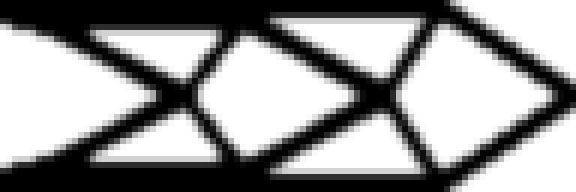
\includegraphics[width=\linewidth]{figures/ch10_v03_cantilever_density.png}
 \end{minipage}
 \hfill
 \begin{minipage}{0.48\textwidth}
  \centering
  
\includegraphics[width=\linewidth]{figures/ch10_v03_half_mbb_density.png}
 \end{minipage}
 \caption{Физическая плотность после SIMP-оптимизации: основная консоль слева и контрольная half-MBB справа. Чёрный цвет соответствует материалу, белый --- пустоте.}
 \label{fig:practical-v03-topologies}
\end{figure}

Рисунок~\ref{fig:practical-v03-topologies} нужен не вместо численной проверки, а вместе с ней. В файле результатов сохраняются объём, податливость, невязка, энергетическое тождество и история итераций. Поэтому визуально правдоподобная топология не может скрыть нарушение физического ограничения или ошибку решателя.

\subsection{Что показывает повторный расчёт на другой сетке}
\label{subsec:practical-v03-mesh-check}

Оптимизация выполнялась только на основной сетке $96\times32$. Чтобы отдельно оценить чувствительность физического расчёта к дискретизации, найденное поле $\rho$ консоли без новой оптимизации переносится на две сетки. Для $48\times16$ каждые четыре плотности усредняются, а для $192\times64$ каждая плотность копируется в четыре дочерних элемента. Средняя плотность при обеих операциях остаётся равной $0.4$.

Повторный FEM даёт
\begin{equation}
\label{eq:practical-v03-mesh-check}
 \begin{aligned}
  J_{48\times16} &= 254.061339,\\
  J_{96\times32} &= 233.550039,\\
  J_{192\times64} &= 239.409264.
 \end{aligned}
\end{equation}
На более тонкой сетке отклонение от основного расчёта составляет 2.51\%. Это не доказательство сеточной сходимости оптимальной топологии: на трёх сетках не решались три независимые задачи оптимизации. Проверка уже по смыслу --- она показывает, насколько меняется точная физическая оценка одного и того же найденного распределения при удвоении и уменьшении разрешения.

Итог проекта~1 теперь содержит полный проверяемый контур
\begin{equation}
 c
 \longrightarrow
 \rho^{(0)}
 \longrightarrow
 \mathrm{FEM}
 \longrightarrow
 \nabla J
 \longrightarrow
 \mathrm{filter+OC}
 \longrightarrow
 \rho^\star
 \longrightarrow
 \mathrm{FEM}.
\end{equation}
Именно этот solver в следующем проекте становится источником данных. Обучаемая модель будет сравниваться не с абстрактной ``правильной картинкой'', а с полями и функционалами, вычисленными здесь.


\section{Проект 2. Нейронный оператор как суррогат физического решателя}
\label{sec:practical-project-neural-operator}

Второй проект не пытается напрямую угадывать оптимальную конструкцию. Его задача уже: заменить многократно вызываемый физический расчёт приближённым отображением
\begin{equation}
\label{eq:practical-v04-operator-map}
 (\rho_h,c)\longmapsto U_h.
\end{equation}
Точный ответ по-прежнему задаётся FEM-системой~\eqref{eq:practical-fem-state}. Поэтому обучаемая модель будет сравниваться с собственным численным эталоном проекта~1, а не с визуальной похожестью полей.

\subsection{Почему в датасете нужны промежуточные конструкции}
\label{subsec:practical-v04-why-trajectories}

Если сохранить только финальные $\rho^\star$, выборка будет состоять в основном из хороших почти бинарных топологий. Однако суррогат нужен также для оценки промежуточных и сгенерированных кандидатов, где плотности могут быть серыми и податливость далека от оптимальной. Поэтому исходной единицей данных становится целая SIMP-траектория при фиксированном условии $c$.

Из каждой траектории выбираются шесть состояний с относительным прогрессом
\begin{equation}
\label{eq:practical-v04-snapshot-fractions}
 0,\qquad
 0.05,\qquad
 0.15,\qquad
 0.35,\qquad
 0.65,\qquad
 1.
\end{equation}
Первый снимок соответствует равномерной начальной плотности, последний --- состоянию после выполнения критерия $\max|\Delta x|<10^{-2}$. Остальные четыре точки покрывают различные стадии перераспределения материала. Верхний предел числа OC-итераций в генераторе равен $800$; это только защитный cap и он не меняет критерий остановки.

\subsection{Семейство условий}
\label{subsec:practical-v04-condition-grid}

Геометрия и закрепление консоли остаются теми же, что в проекте~1. Варьируются объёмная доля, высота точки приложения силы и её направление:
\begin{equation}
\label{eq:practical-v04-condition-grid}
 \begin{aligned}
 f_{\mathrm{vol}}
 &\in\{0.30,0.40,0.50\},\\
 y_F/H
 &\in\{0.25,0.50,0.75\},\\
 \theta_F
 &\in\{-105^\circ,-90^\circ,-75^\circ\}.
 \end{aligned}
\end{equation}
Полный декартов набор содержит $27$ условий. Угол в компактных метаданных кодируется парой $(\cos\theta_F,\sin\theta_F)$, поэтому
\begin{equation}
 q=
 \left(
 f_{\mathrm{vol}},
 \frac{y_F}{H},
 \cos\theta_F,
 \sin\theta_F
 \right).
\end{equation}

Все 27 траекторий достигли критерия остановки за $77$--$324$ OC-итерации; лимит $800$ ни разу не сработал. Максимальная относительная FEM-невязка сохранённых состояний равна $2.34e-12$.34e-12.

\subsection{Схема одного sample}
\label{subsec:practical-v04-sample-schema}

Физическая плотность естественно определена на элементах и имеет размер $32\times96$. Поле перемещений определено в узлах и имеет два компонента на сетке $33\times97$. Поэтому \texttt{rho\_element} хранит исходную физическую плотность, а \texttt{rho\_node} --- её локальное усреднение в узлы. Второе представление не заменяет первое; оно только переводит вход на ту же пространственную сетку, где задано целевое поле.

Сила хранится как два разреженных узловых канала, а два канала маски закреплений постоянны для всего семейства консолей. Цель имеет форму
\begin{equation}
 U_{\mathrm{data}}
 \in
 \mathbb{R}^{2\times33\times97}.
\end{equation}
Дополнительно сохраняются податливость, FEM-невязка, номер исходного условия, номер SIMP-итерации и относительный прогресс по траектории.

\subsection{Разделение без утечки траекторий}
\label{subsec:practical-v04-split}

Снимки одной SIMP-траектории близки, поэтому разделение выполняется по условиям $c$, а не по отдельным состояниям. Все шесть снимков одного условия целиком попадают в train, validation или test.

Из $27$ условий 18 используются для обучения, 4 для validation и 5 для test. При шести снимках на условие получаем
\begin{equation}
\label{eq:practical-v04-split-counts}
 N_{\mathrm{train}}=108,
 \qquad
 N_{\mathrm{val}}=24,
 \qquad
 N_{\mathrm{test}}=30,
\end{equation}
то есть всего 162 точных пар $(\rho_h,c,U_h)$. Автоматический аудит дополнительно проверяет, что один \texttt{condition\_id} никогда не встречается более чем в одном split.

\begin{figure}[ht]
 \centering
 
\includegraphics[width=\textwidth]{figures/ch10_v04_dataset_trajectory.png}
 \caption{Шесть сохранённых состояний одной SIMP-траектории для $f_{\mathrm{vol}}=0.4$, $y_F/H=0.5$, $\theta_F=-90^\circ$: от равномерной начальной плотности до терминальной конструкции.}
 \label{fig:practical-v04-trajectory}
\end{figure}

Рисунок~\ref{fig:practical-v04-trajectory} показывает, что будущая модель видит не только почти чёрно-белые оптимумы, но и промежуточные поля. Это соответствует её практической роли: быстро оценивать произвольный кандидат до дорогой окончательной физической проверки.

\subsection{Воспроизводимость датасета}
\label{subsec:practical-v04-reproducibility}

Полный бинарный датасет не сохраняется в Git. Он генерируется в каталоге \texttt{code/chapter10/data/} под именем \texttt{v04\_operator\_dataset.npz}. Его размер 5.34 MiB и SHA256
\begin{equation}
\label{eq:practical-v04-dataset-hash}
 \begin{gathered}
  \texttt{eeace8c3e22dd1ce0d3cb52bc05c0215}\\
  \texttt{88a948b02e2c74afc84545407f547385}.
 \end{gathered}
\end{equation}
В репозитории остаются генератор, список условий, seed разбиения, schema массивов и manifest с этим хешем. Поэтому данные можно воспроизвести и проверить, не превращая Git в хранилище бинарных обучающих массивов.

Следующий шаг использует именно этот train/validation/test split. Качество суррогата будет измеряться на условиях, исключённых из обучения, по относительной ошибке поля, ошибке податливости и физической невязке после подстановки предсказанного $U_h$ в точную FEM-систему.

\subsection{Fourier Neural Operator}
\label{subsec:practical-v05-fno}

После V04 вход и точный выход уже имеют согласованную пространственную структуру. Для суррогата используется компактный Fourier Neural Operator. В каждом скрытом слое локальное преобразование складывается со спектральным:
\begin{equation}
\label{eq:practical-v05-fno-layer}
 v_{k+1}
 =
 \sigma\!\left(
 W_k v_k
 +
 \mathcal{F}^{-1}
 \!\left[
 R_k\,\mathcal{F}v_k
 \right]
 \right).
\end{equation}
Здесь сохраняются только низкие Fourier-моды: $8$ по вертикальной и $16$ по горизонтальной координате. Ширина скрытого представления равна $24$, число Fourier-слоёв --- четыре. В итоге модель содержит 1184018 обучаемых действительных параметров.

Пространственный вход имеет девять каналов:
\begin{equation}
\label{eq:practical-v05-input}
 X_h=
 \left(
 \rho_h,\,
 F_x,\,
 F_y,\,
 x/L,\,
 y/H,\,
 f_{\mathrm{vol}},\,
 y_F/H,\,
 \cos\theta_F,\,
 \sin\theta_F
 \right).
\end{equation}
Последние четыре величины постоянны по пространству для одного sample. Выход содержит два канала $(\widehat u_x,\widehat u_y)$. Левое закрепление не изучается статистически: после последнего слоя выход умножается на маску свободных узлов, поэтому $\widehat u_x=\widehat u_y=0$ при $x=0$ выполняется точно.

\subsection{Обучение без доступа к test}
\label{subsec:practical-v05-training}

Статистики нормировки вычисляются только по $108$ train samples. Validation содержит $24$ состояния и выбирает checkpoint; $30$ test samples не участвуют ни в нормировке, ни в early stopping.

Оптимизация выполняется AdamW с начальным шагом $10^{-3}$ и weight decay $10^{-4}$. При отсутствии улучшения validation loss шаг уменьшается, а обучение останавливается досрочно. Лучший checkpoint получен на эпохе 160; всего выполнено 205 эпох. Минимальная validation-ошибка в нормированных переменных равна 0.0841. Полное обучение на CPU заняло 24.48 мин.

\subsection{Ошибка поля и инженерных величин}
\label{subsec:practical-v05-test}

Основная test-метрика вычисляется в физических перемещениях,
\begin{equation}
\label{eq:practical-v05-field-error}
 e_U
 =
 \frac{
 \norm{\widehat U_h-U_h}_2
 }{
 \norm{U_h}_2
 }.
\end{equation}
На $30$ test samples медиана $e_U$ равна 0.0368, а $90$-й процентиль --- 0.0919. Эти условия целиком отсутствовали в train split, поэтому результат нельзя объяснить запоминанием соседних состояний той же SIMP-траектории.

Для инженерной проверки одного совпадения формы поля недостаточно. По известному вектору нагрузки податливость FNO-предсказания вычисляется без нового FEM-решения:
\begin{equation}
 \widehat J_h
 =
 F_h^{\trans}\widehat U_h,
 \qquad
 e_J
 =
 \frac{
 |\widehat J_h-J_h|
 }{
 |J_h|
 }.
\end{equation}
Медианная относительная ошибка $e_J$ составляет 0.0733, $90$-й процентиль --- 0.2088.

Более строгая проверка подставляет предсказанное поле обратно в точную матрицу жёсткости:
\begin{equation}
\label{eq:practical-v05-physics-residual}
 r_{\mathrm{FNO}}
 =
 \frac{
 \norm{
 K_{ff}(\rho_h)\widehat U_f-F_f
 }_2
 }{
 \norm{F_f}_2
 }.
\end{equation}
Медиана этой невязки равна 6.45e+01, а $90$-й процентиль --- 8.64e+01. В отличие от ошибки поля, эта величина напрямую проверяет локальное равновесие. Поэтому малый $e_U$ сам по себе ещё не делает нейронный ответ заменой окончательной FEM-верификации.

\begin{figure}[ht]
 \centering
 
\includegraphics[width=\textwidth]{figures/ch10_v05_fno_test_example.png}
 \caption{Test-пример с ошибкой поля, близкой к медианной: слева точный модуль перемещения, в центре FNO-предсказание, справа модуль ошибки. Для первых двух панелей используется общий масштаб.}
 \label{fig:practical-v05-fno-example}
\end{figure}

\subsection{Стоимость и перенос разрешения}
\label{subsec:practical-v05-resolution}

На одном CPU и одном состоянии сетки $96\times32$ измеренный forward FNO занимает 32.553 мс, а полная сборка и решение FEM --- 171.536 мс. Их отношение в этом локальном измерении равно 5.27. Это не аппаратно-независимая оценка сложности, а практический wall-clock контроль конкретной реализации.

Fourier-слои не содержат параметров, привязанных к числу узлов, поэтому тот же checkpoint можно технически вызвать на другой регулярной сетке. Для exploratory-проверки одна терминальная test-конструкция перенесена с $96\times32$ на $192\times64$ элементов и повторно решена точным FEM. Без какого-либо fine-resolution обучения FNO дал
\begin{equation}
\label{eq:practical-v05-resolution-transfer}
 e_U^{192\times64}
 =
 0.3595,
 \qquad
 e_J^{192\times64}
 =
 0.2819.
\end{equation}
Физическая невязка на этой сетке равна 3.20e+02. Этот опыт проверяет возможность прямого вызова оператора на другом разрешении, но сам по себе не доказывает resolution invariance: для такого вывода нужен систематический эксперимент по нескольким условиям и сеткам.

Локальный checkpoint не хранится в Git. Его SHA256 разбит на две строки:
\begin{equation}
\label{eq:practical-v05-checkpoint-hash}
 \begin{gathered}
  \texttt{e3154c0cb697ee3abe8e9e83e7033ab9}\\
  \texttt{cf52f17495e98e431deeda17184e1608}.
 \end{gathered}
\end{equation}
В репозитории остаются архитектура, seed, история обучения и все test-метрики. Поэтому следующий шаг может отдельно разобрать зависимость ошибок от стадии SIMP, условия нагрузки и требуемой точности, не меняя уже обученный baseline.

\subsection{Где ошибается суррогат}
\label{subsec:practical-v06-error-structure}

После обучения архитектура и checkpoint больше не меняются. V06 повторно прогоняет те же $30$ test-состояний и разбивает ошибку по положению внутри SIMP-траектории. Это отделяет качество модели от процедуры выбора checkpoint.

\begin{table}[ht]
 \centering
 \small
 \begin{tabular}{c|c|c|c}
  прогресс & медиана $e_U$ & медиана $e_J$ & медиана $r_{\mathrm{FNO}}$\\
  \hline
  0.00 & 3.30\% & 3.85\% & 6.95e+01\\
  0.05 & 4.29\% & 6.96\% & 6.11e+01\\
  0.15 & 3.96\% & 8.08\% & 7.22e+01\\
  0.35 & 3.49\% & 7.98\% & 6.59e+01\\
  0.65 & 3.52\% & 7.70\% & 6.31e+01\\
  1.00 & 3.80\% & 7.69\% & 6.23e+01\\
 \end{tabular}
 \caption{Ошибка фиксированного FNO на шести стадиях test-траекторий. На каждой стадии присутствуют пять независимых условий.}
 \label{tab:practical-v06-stage-errors}
\end{table}

Минимальная медианная ошибка поля наблюдается на стадии 0, максимальная --- на стадии 1. Поэтому единственного числа $e_U$ недостаточно для описания качества: распределение конструкций меняется по мере SIMP-оптимизации, а вместе с ним меняется и трудность surrogate-задачи.

\subsection{Пять невидимых условий}
\label{subsec:practical-v06-condition-generalization}

Каждое test-условие содержит шесть состояний одной траектории. Полученные ошибки приведены отдельно:
\begin{table}[ht]
 \centering
 \small
 \begin{tabular}{c|c|c|c|c|c}
  $f_{\mathrm{vol}}$ & $y_F/H$ & $\theta_F$ & med $e_U$ & med $e_J$ & порядок $J$\\
  \hline
  0.30 & 0.50 & $-90^\circ$ & 2.79\% & 0.89\% & 100.0\%\\
  0.40 & 0.25 & $-90^\circ$ & 3.54\% & 1.66\% & 100.0\%\\
  0.40 & 0.25 & $-75^\circ$ & 9.60\% & 19.64\% & 73.3\%\\
  0.50 & 0.25 & $-90^\circ$ & 4.00\% & 7.69\% & 100.0\%\\
  0.50 & 0.75 & $-75^\circ$ & 2.98\% & 14.87\% & 100.0\%\\
 \end{tabular}
 \caption{Condition-level test: медианные ошибки и доля правильно упорядоченных пар кандидатов по податливости внутри одного условия.}
 \label{tab:practical-v06-condition-errors}
\end{table}

Эти пять строк нельзя интерпретировать как независимый эксперимент по влиянию $f_{\mathrm{vol}}$, положения силы или угла. Test subset специально отделён от train, но содержит только пять несбалансированных комбинаций параметров. Поэтому таблица показывает различия между конкретными невидимыми условиями, а не причинный эффект каждого параметра по отдельности.

\subsection{Почему малой ошибки поля недостаточно}
\label{subsec:practical-v06-physics-gap}

Для точного решения на свободных степенях свободы $K_{ff}U_f=F_f$. Если $\widehat U_f=U_f+\delta U_f$, то невязка surrogate равна
\begin{equation}
\label{eq:practical-v06-residual-error-link}
 K_{ff}\widehat U_f-F_f
 =
 K_{ff}\delta U_f.
\end{equation}
Поэтому относительная евклидова ошибка $\norm{\delta U}_2/\norm{U}_2$ и ошибка равновесия измеряют разные свойства. Матрица жёсткости усиливает те компоненты ошибки, которые дороги в энергетической норме. Именно поэтому медиана $e_U=0.0368$ может сосуществовать с медианной физической невязкой $64.5$.

На $30$ test samples корреляция между $e_U$ и $e_J$ равна 0.619, а между $e_U$ и $\log_{10}r_{\mathrm{FNO}}$ --- 0.466. Даже если эти величины меняются согласованно, ни одна из первых двух метрик не заменяет прямую проверку уравнения равновесия.

\subsection{Полезность как дешёвого фильтра}
\label{subsec:practical-v06-screening}

Для предварительного отбора кандидатов важна не только абсолютная точность податливости, но и сохранение порядка. В каждом из пяти test-условий имеются шесть состояний, поэтому можно сравнить все пары конструкций по точному $J_h$ и по $\widehat J_h=F_h^{\trans}\widehat U_h$.

FNO правильно сохраняет порядок в 94.7\% пар. Лучший из шести snapshots выбран правильно в 4 из $5$ условий, а знак улучшения от начального состояния к терминальному определён правильно в 5 из $5$ случаев. Это более узкая и практически полезная роль, чем замена FEM: surrogate может быстро ранжировать или отбрасывать кандидатов, после чего небольшое число лучших решений проверяется точной механикой.

Из V05 сохраняется и вычислительная причина такого использования: один CPU-forward был примерно в 5.27 раза быстрее полной FEM-сборки и решения. Но граница обобщения также остаётся прежней: zero-shot ошибка поля на $192\times64$ составляла 35.95\%. Поэтому ускорение на основной сетке не является доказательством ни физической состоятельности, ни независимости от разрешения.

В результате проект~2 даёт не замену численной механике, а двухуровневую схему:
\begin{equation}
\label{eq:practical-v06-screening-pipeline}
 \text{много кандидатов}
 \xrightarrow{\mathrm{FNO}}
 \text{короткий список}
 \xrightarrow{\mathrm{FEM}}
 \text{физически проверенный результат}.
\end{equation}
Именно такой режим будет использоваться дальше: генеративная модель может предлагать конструкции быстро, но окончательные инженерные метрики вычисляются точным FEM.

\section{Проект 3. Условная диффузионная генерация с физическим уточнением}

\subsection{Почему генератор работает на уменьшенной сетке}
\label{subsec:practical-v07-grid}

В третьем проекте генеративная модель не заменяет оптимизатор и не выдаёт окончательный инженерный ответ. Её задача уже: быстро предложить несколько пространственно различных начальных плотностей для заданной нагрузки. Поэтому перед обучением поле $32\times96$ усредняется блоками $2\times2$:
\begin{equation}
\label{eq:practical-v07-downsample}
 \rho^{48\times16}_{ij}
 =
 \frac{1}{4}
 \sum_{a=0}^{1}
 \sum_{b=0}^{1}
 \rho^{96\times32}_{2i+a,\,2j+b}.
\end{equation}
Такое преобразование точно сохраняет среднюю плотность, а число элементов генеративного поля уменьшается с $3072$ до $768$.

\subsection{Условие и diffusion-задача}
\label{subsec:practical-v07-condition}

Engineering condition остаётся тем же:
\begin{equation}
 \left(
 f_{\mathrm{vol}},
 y_F/H,
 \cos\theta_F,
 \sin\theta_F
 \right).
\end{equation}
Однако train split содержит шесть состояний одной SIMP-траектории. Если не сообщить модели, на какой стадии получено поле, одному и тому же engineering condition будут соответствовать и почти однородная начальная плотность, и поздняя топология. Поэтому только во время обучения добавляется пятая координата $s\in[0,1]$ --- прогресс SIMP. При генерации всегда задаётся $s=1$.

Плотность переводится в диапазон $[-1,1]$, после чего используется дискретный diffusion-процесс
\begin{equation}
\label{eq:practical-v07-forward}
 x_t
 =
 \sqrt{\bar\alpha_t}\,x_0
 +
 \sqrt{1-\bar\alpha_t}\,\varepsilon,
 \qquad
 \varepsilon\sim\mathcal N(0,I).
\end{equation}
Conditional U-Net получает $x_t$, timestep $t$ и пятикомпонентное условие и предсказывает шум $\widehat\varepsilon_\theta$. Число diffusion steps равно $100$, число параметров denoiser --- 797249.

\subsection{Обучение conditional DDPM}
\label{subsec:practical-v07-training}

Condition-level split из V04 сохраняется без изменений: $108$ train, $24$ validation и $30$ test samples. Нормировка condition вычисляется только по train. Используются AdamW, exponential moving average параметров и early stopping по фиксированной validation noise MSE. Лучший checkpoint получен на эпохе 139; всего выполнено 194 эпох. Минимальная validation noise MSE равна 0.1140, а диагностическая test noise MSE --- 0.0882. Обучение на CPU заняло 9.55 мин.

\subsection{Генерация невидимых условий}
\label{subsec:practical-v07-sampling}

Для каждого из пяти test conditions генерируется по $16$ полей при $s=1$, всего $80$ кандидатов. До какой-либо физической коррекции медианная абсолютная ошибка средней плотности составляет 3.90\%, $90$-й процентиль --- 9.61\%. Это непосредственно показывает, насколько хорошо diffusion-модель сама усвоила условие по объёму.

Для следующего шага нужна точная допустимость по материалу. Поэтому применяется одномерная проекция
\begin{equation}
\label{eq:practical-v07-volume-projection}
 \begin{aligned}
  \widetilde\rho_e
  &=
  \mathrm{clip}_{[0,1]}
  \left(
  \rho_e+\lambda
  \right),
  \\
  \frac{1}{N_e}
  \sum_e
  \widetilde\rho_e
  &=
  f_{\mathrm{vol}}.
 \end{aligned}
\end{equation}
где $\lambda$ находится бисекцией. Максимальная ошибка объёмной доли после этой операции равна 1.19e-07. Проекция не использует механику и не улучшает compliance; она только переводит сгенерированное поле в допустимый по объёму класс.

\begin{figure}[ht]
 \centering
 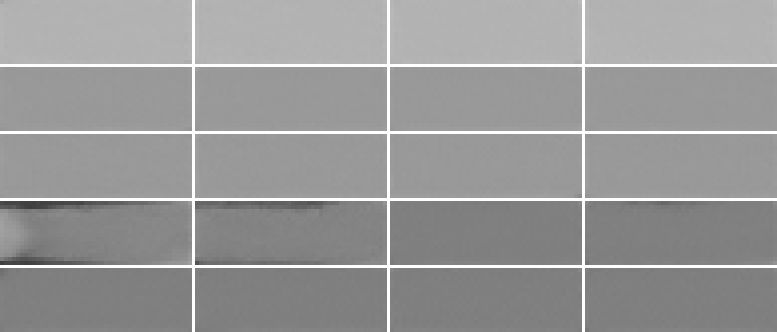
\includegraphics[width=\textwidth]{figures/ch10_v07_diffusion_candidates.png}
 \caption{По четыре volume-projected кандидата для каждого из пяти невидимых test conditions. Строки соответствуют условиям, столбцы --- различным diffusion samples.}
 \label{fig:practical-v07-candidates}
\end{figure}

\subsection{Разнообразие и степень бинарности}
\label{subsec:practical-v07-diversity}

Среднее попарное RMS-расстояние кандидатов внутри одного условия используется как простая проверка collapse. Его медиана по пяти условиям равна 0.0355. Следовательно, разные шумовые старты не сводятся к одному и тому же полю.

Для оценки серости используется
\begin{equation}
\label{eq:practical-v07-binarity}
 b(\rho)
 =
 \frac{1}{N_e}
 \sum_e
 4\rho_e(1-\rho_e).
\end{equation}
Здесь $b=0$ для бинарного поля и $b=1$ для однородного $\rho=1/2$. У generated candidates медиана $b$ равна 0.9599, а у терминальных test-топологий SIMP после такого же downsampling --- 0.2678. Это число не трактуется как критерий инженерной пригодности: оно только показывает, насколько diffusion output по серости похож на поздние SIMP-состояния.

Медианное RMS-расстояние сгенерированного кандидата до ближайшей терминальной train-топологии равно 0.3879. Эта величина также не доказывает новизну конструкции, но позволяет проверить, что sampling не сводится к точному воспроизведению одного сохранённого train-поля.

\subsection{Что V07 ещё не проверяет}
\label{subsec:practical-v07-boundary}

На этом шаге к generated candidates намеренно не применяется FEM. Поэтому из рисунка, разнообразия или noise MSE нельзя делать вывод о compliance, связности или механической допустимости. V07 заканчивается набором volume-feasible стартовых плотностей, а инженерная проверка переносится в V08:
\begin{equation}
\label{eq:practical-v07-next-pipeline}
 \begin{gathered}
  \text{conditional DDPM}
  \longrightarrow
  \text{volume projection}
  \\
  \longrightarrow
  \text{exact FEM}
  \\
  \longrightarrow
  \text{few-step SIMP refinement}.
 \end{gathered}
\end{equation}
Так генеративная модель отвечает только за предложение кандидатов, а физический смысл результата остаётся проверяемой частью вычислительного конвейера.

Локальный checkpoint и массив $80$ кандидатов не хранятся в Git. Их SHA256 вместе с параметрами обучения и sampling сохранены в 	exttt{v07\_diffusion\_results.json} и проверяются скриптом аудита.


\label{sec:practical-project-diffusion}

Третий проект меняет тип задачи. Теперь требуется по условию $c$ породить распределение разумных проектных кандидатов,
\begin{equation}
\label{eq:practical-conditional-generator}
 (z,c)
 \xmapsto{\ G_\phi\ }
 \rho_h^{\mathrm{gen}},
\end{equation}
где $z$ содержит случайность генерации. Условная диффузионная модель обучается на конструкциях, полученных из проверенного физического pipeline проекта~1. Сгенерированная плотность не объявляется решением до проверки точным FEM.

Практический контур проекта имеет вид
\begin{equation}
\label{eq:practical-generative-refinement}
 (z,c)
 \xmapsto{\ G_\phi\ }
 \rho_h^{\mathrm{gen}}
 \xmapsto{\ \mathrm{FEM}\ }
 J_h^{\mathrm{gen}}
 \longrightarrow
 \text{короткое SIMP-уточнение}
 \longrightarrow
 \rho_h^{\mathrm{ref}}
 \xmapsto{\ \mathrm{FEM}\ }
 J_h^{\mathrm{ref}}.
\end{equation}
Смысл такого эксперимента не в том, чтобы доказать превосходство генеративной модели над SIMP заранее. Проверяется более узкий практический вопрос: способен ли генератор быстро предлагать разнообразные начальные конструкции, которые после точной физической оценки и небольшого числа классических шагов дают конкурентный результат.

\subsection{Точная FEM-проверка всех кандидатов}
\label{subsec:practical-v08-screening}

V07 оставил $80$ допустимых по объёмной доле полей на сетке $48\times16$. Перед механической оценкой каждое поле поднимается на основную сетку без интерполяционного сглаживания:
\begin{equation}
\label{eq:practical-v08-upsample}
 \rho^{96\times32}_{2i+a,\,2j+b}
 =
 \rho^{48\times16}_{ij},
 \qquad
 a,b\in\{0,1\}.
\end{equation}
Средняя плотность при этом не меняется. После подъёма для каждого кандидата собирается точная матрица жёсткости с тем же $p=3$ и $E_{\min}/E_0=10^{-9}$, что и в проекте~1, и заново решается FEM-задача. Поэтому ranking строится не по изображению и не по нейросетевому surrogate, а по точному $J_h=F_h^{\trans}U_h$.

Для всех $80$ расчётов максимальная ошибка объёмной доли составила 1.00e-07, максимальная относительная FEM-невязка --- 2.40e-12. Пороговый путь материала от закрепления к нагруженной границе при $\rho\ge 0.5$ имели 6 из $80$ полей. Последнее число используется только как описательная проверка структуры: механическая допустимость всё равно определяется FEM.

\subsection{Одинаковый бюджет уточнения}
\label{subsec:practical-v08-budget}

В каждом test condition из $16$ полей выбираются четыре кандидата с наименьшим exact FEM compliance. Каждый из них получает ровно $30$ OC/SIMP updates с $r_{\min}=1.5$ и move limit $0.2$. Для контроля в том же условии выполняются те же $30$ updates от стандартной однородной инициализации $\rho=f_{\mathrm{vol}}$:
\begin{equation}
\label{eq:practical-v08-fixed-budget}
 \begin{aligned}
  \rho^{\mathrm{gen}}
  &\xrightarrow{\ 30\ \mathrm{OC}\ }
  \rho^{\mathrm{ref}},
  \\
  \rho^{\mathrm{uni}}
  &\xrightarrow{\ 30\ \mathrm{OC}\ }
  \rho_{30}^{\mathrm{uni}}.
 \end{aligned}
\end{equation}
Таким образом, сравнение warm start и обычного старта имеет одинаковый оптимизационный бюджет. Полностью сошедшееся terminal SIMP-состояние V04 используется отдельно как reference, а не как участник 30-шагового сравнения.

\subsection{Что получилось после 30 шагов}
\label{subsec:practical-v08-results}

\begin{table}[ht]
 \centering
 \small
 \begin{tabular}{c|r|r|r|r}
  $c$ & $J_{\mathrm{gen}}$ & $J_{\mathrm{ref}}$ & $J_{30}^{\mathrm{uni}}$ & $J_{\star}$\\
  \hline
  4 & 4342.92 & 339.59 & 340.28 & 335.70\\
  10 & 1517.15 & 246.12 & 247.39 & 240.09\\
  11 & 760.43 & 216.74 & 215.10 & 210.51\\
  19 & 465.90 & 192.35 & 192.11 & 189.18\\
  26 & 321.08 & 189.62 & 191.43 & 187.36\\
 \end{tabular}
 \caption{Для каждого невидимого условия: лучший сгенерированный кандидат до уточнения, лучший из четырёх после $30$ шагов, однородный $30$-шаговый контроль и сошедшийся SIMP reference из V04.}
 \label{tab:practical-v08-compliance}
\end{table}

В 3 из $5$ условий лучший diffusion warm start после одинаковых $30$ шагов имеет меньшую податливость, чем однородный $30$-шаговый контроль. Медиана отношения
\[
 \frac{J_{\mathrm{ref}}}{J_{30}^{\mathrm{uni}}}
 =
 0.9980,
\]
а медиана $J_{\mathrm{ref}}/J_{\star}$ равна 1.0168. Для самого однородного 30-шагового контроля медиана $J_{30}^{\mathrm{uni}}/J_{\star}$ равна 1.0217. Эти три числа разделяют эффект инициализации и эффект полного доведения SIMP до сходимости.

По всем $20$ уточняемым кандидатам медиана $J_{\mathrm{ref}}/J_{\mathrm{gen}}$ равна 0.1859. Следовательно, основное снижение compliance происходит уже внутри физического refinement, а роль DDPM проверяется более строго: даёт ли он старт, который при том же числе шагов оказывается лучше стандартного старта.

\begin{figure}[ht]
 \centering
 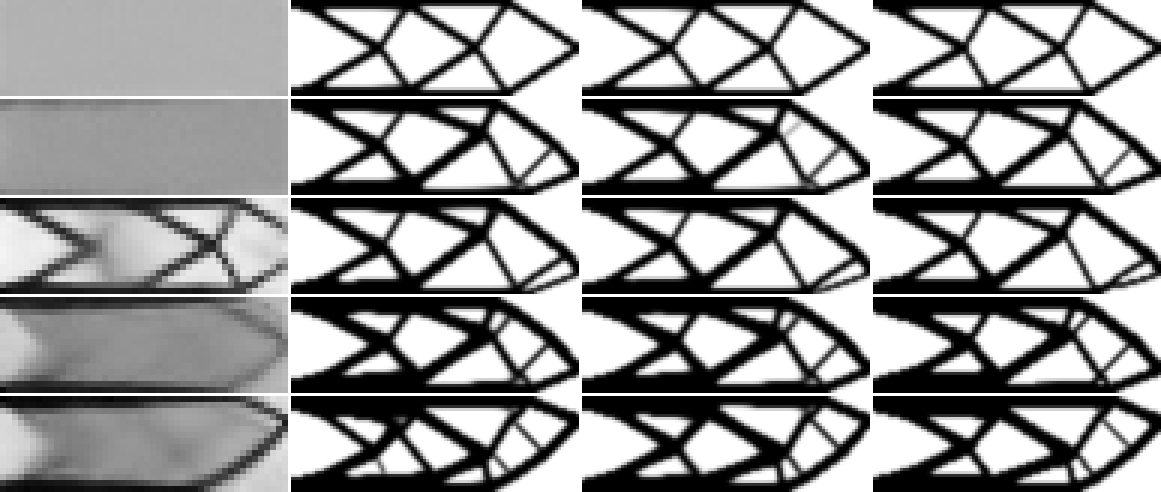
\includegraphics[width=\textwidth]{figures/ch10_v08_fem_refinement.png}
 \caption{Пять test conditions, по одному на строку. Столбцы слева направо: лучший кандидат после exact FEM screening, лучший diffusion warm start после $30$ SIMP-шагов, однородный $30$-шаговый контроль и terminal SIMP reference.}
 \label{fig:practical-v08-refinement}
\end{figure}

\subsection{Серость, связность и величина коррекции}
\label{subsec:practical-v08-structure}

Медианная бинарность выбранных diffusion starts равна 0.9222, после $30$ шагов --- 0.2174, а у terminal SIMP references --- 0.2046. Пороговая связность при $\rho\ge0.5$ наблюдалась у 2 из $20$ выбранных starts и у 20 из $20$ полей после refinement.

Медианное RMS-изменение плотности за $30$ шагов равно 0.4045. Это число важно вместе с compliance: если поле меняется существенно, нельзя приписывать конечную конструкцию одному генератору. В нашем pipeline DDPM предлагает начальное состояние, а SIMP и FEM отвечают за физическое исправление и окончательную оценку.

\subsection{Практический вывод проекта 3}
\label{subsec:practical-v08-conclusion}

На этом конечном test-наборе diffusion warm start даёт измеримое преимущество при одинаковом 30-шаговом бюджете. Это не утверждение о глобальном превосходстве DDPM, а результат ровно для пяти заранее отделённых условий.

При этом fixed-budget результат нельзя смешивать с fully converged reference. Даже лучший diffusion warm start после 30 шагов в медиане остаётся выше сошедшегося V04 reference, поэтому короткое уточнение не заменяет полную оптимизацию.

Итоговый вычислительный контракт проекта~3 теперь полностью проверяем:
\begin{equation}
\label{eq:practical-v08-final-pipeline}
 \begin{gathered}
  c
  \longrightarrow
  \text{conditional DDPM candidates}
  \longrightarrow
  \text{exact FEM ranking}
  \\
  \longrightarrow
  \text{fixed-budget SIMP refinement}
  \longrightarrow
  \text{final exact FEM}.
 \end{gathered}
\end{equation}
Генератор не получает права объявлять конструкцию хорошей самостоятельно; это право остаётся у физического расчёта и явно заданного критерия сравнения.

\section{Сквозное сравнение и границы применимости}
\label{sec:practical-cross-project-comparison}

После трёх проектов сравниваются три режима вычисления одной и той же инженерной задачи. Первый режим решает физику и оптимизацию напрямую; второй заменяет многократный физический расчёт обучаемым оператором там, где его ошибка допустима; третий использует обучаемую модель для поиска кандидатов, но возвращает точную физику в окончательную проверку. Сравнение проводится по качеству конструкции, численной допустимости, времени и области условий, на которой метод был проверен.

Главный результат главы --- воспроизводимый вычислительный маршрут. Для нового условия задачи должно быть явно указано, как формируется $c$ и какой решатель вычисляет $U_h$. Обучаемое приближение отделяется от точного расчёта, а окончательное качество всегда определяется заранее выбранным физическим критерием.

\subsection{Три разных роли в одном вычислительном контуре}
\label{subsec:practical-v09-three-roles}

Три проекта нельзя сравнивать как три взаимозаменяемых решателя. В первом проекте FEM вычисляет физический ответ, а SIMP непосредственно меняет конструкцию. Во втором проекте FNO приближает отображение $\rho_h,c\mapsto U_h$ и потому может ускорять повторную оценку поля, но не получает права заменить уравнение равновесия. В третьем проекте DDPM вообще не решает механику: он предлагает стартовые плотности, после чего точный FEM и SIMP возвращаются в контур.

Для основной консоли классический SIMP уменьшил податливость с 1848.075 до 233.550, то есть на 87.36\%. Сходимость потребовала 77 итераций. Этот результат остаётся baseline, потому что каждая оптимизационная итерация опирается на тот же проверенный FEM, которым затем оцениваются ML-кандидаты.

\subsection{Что действительно дал нейронный оператор}
\label{subsec:practical-v09-fno-role}

На condition-level test медианная относительная ошибка поля FNO равна 3.68\%, а медианная ошибка податливости --- 7.33\%. Один CPU-forward оказался примерно в 5.27 раза быстрее полного FEM-расчёта на сетке $96\times32$. Для screening важнее, что внутри test-условий FNO сохранил правильный порядок по податливости в 94.7\% пар и выбрал лучший snapshot в 4 случаях из 5.

Однако медианная невязка равновесия равна 6.45e+01, а zero-shot ошибка поля на $192\times64$ --- 35.95\%. Поэтому практический вывод узкий: FNO полезен для быстрого предварительного ранжирования на проверенном распределении условий и разрешении, но окончательная инженерная метрика должна возвращаться к exact FEM.

\subsection{Что действительно дала условная диффузия}
\label{subsec:practical-v09-ddpm-role}

DDPM генерирует разнообразные поля, но raw candidates не являются готовыми конструкциями. До refinement при пороге $\rho=0.5$ связны только 6 из 80 полей. После exact FEM screening и $30$ SIMP-шагов для top-$4$ кандидатов связны уже 20 из 20. Медианная бинарность меняется с 0.960 до 0.217, тогда как у fully converged terminal reference она равна 0.205.

Главная проверка warm start сравнивает одинаковый бюджет в $30$ SIMP-шагов. Diffusion initialization лучше обычной однородной инициализации в 3 из 5 условий, но медианное отношение
\begin{equation}
\label{eq:practical-v09-warmstart-ratio}
 \frac{J_{\mathrm{diffusion}+30}}
 {J_{\mathrm{uniform}+30}}
 =
 0.99798.
\end{equation}
Это преимущество невелико. Одновременно
\begin{equation}
\label{eq:practical-v09-terminal-gap}
 \frac{J_{\mathrm{diffusion}+30}}
 {J_{\mathrm{terminal}}}
 =
 1.01677,
\end{equation}
а медианное RMS-изменение плотности за refinement равно 0.404. Следовательно, генератор влияет на начальную точку, но основную перестройку до механически пригодной конструкции по-прежнему выполняет SIMP.

\subsection{Сквозной практический маршрут}
\label{subsec:practical-v09-route}

Полученный вычислительный маршрут можно записать без смешения ролей:
\begin{equation}
\label{eq:practical-v09-final-route}
 \begin{gathered}
  c,\rho
  \longrightarrow
  \text{FNO screening}
  \longrightarrow
  \text{короткий список},
  \\
  c
  \longrightarrow
  \text{DDPM candidates}
  \longrightarrow
  \text{FEM screening}
  \longrightarrow
  \text{SIMP refinement},
  \\
  \text{любой финальный кандидат}
  \longrightarrow
  \text{exact FEM}.
 \end{gathered}
\end{equation}
Первый ML-блок ускоряет оценку, второй расширяет поиск начальных конструкций, но физическая проверка в обоих случаях возвращается в точный решатель. Именно это является общим инженерным выводом трёх проектов.

\subsection{Стоимость и границы утверждений}
\label{subsec:practical-v09-cost-scope}

Обучение FNO заняло 24.48 мин CPU-времени, обучение DDPM --- 9.55 мин, а полный V08 screening и refinement --- 1.92 мин. Эти времена относятся к одному ноутбуку и не являются оценками асимптотической сложности. Они нужны только для воспроизводимого сравнения внутри данного эксперимента.

Полученные числа не дают оснований утверждать инвариантность FNO к разрешению, универсальное преимущество диффузионной инициализации или причинное влияние отдельных параметров нагрузки. В тестовой части всего пять новых условий, а перенос FNO на более тонкую сетку заметно ухудшил точность. Поэтому результат главы скромнее и практически важнее: обучаемые модели можно включать в расчётный контур только с возвратом к точной физической проверке.

\subsection{Воспроизводимость V09}
\label{subsec:practical-v09-reproducibility}

Численные выводы V03--V08 собраны в сводном файле V09. Отдельный манифест хранит контрольные суммы пяти файлов результатов и пяти локальных артефактов: датасета, двух контрольных точек моделей и двух массивов кандидатов. Новых экспериментов V09 не добавляет. На этапе CLOSE остаются только итоговый аудит, сборка PDF и создание единственного архива.


\end{document}
